\documentclass[twoside]{book}

% Packages required by doxygen
\usepackage{fixltx2e}
\usepackage{calc}
\usepackage{doxygen}
\usepackage[export]{adjustbox} % also loads graphicx
\usepackage{graphicx}
\usepackage[utf8]{inputenc}
\usepackage{makeidx}
\usepackage{multicol}
\usepackage{multirow}
\PassOptionsToPackage{warn}{textcomp}
\usepackage{textcomp}
\usepackage[nointegrals]{wasysym}
\usepackage[table]{xcolor}

% Font selection
\usepackage[T1]{fontenc}
\usepackage[scaled=.90]{helvet}
\usepackage{courier}
\usepackage{amssymb}
\usepackage{sectsty}
\renewcommand{\familydefault}{\sfdefault}
\allsectionsfont{%
  \fontseries{bc}\selectfont%
  \color{darkgray}%
}
\renewcommand{\DoxyLabelFont}{%
  \fontseries{bc}\selectfont%
  \color{darkgray}%
}
\newcommand{\+}{\discretionary{\mbox{\scriptsize$\hookleftarrow$}}{}{}}

% Page & text layout
\usepackage{geometry}
\geometry{%
  a4paper,%
  top=2.5cm,%
  bottom=2.5cm,%
  left=2.5cm,%
  right=2.5cm%
}
\tolerance=750
\hfuzz=15pt
\hbadness=750
\setlength{\emergencystretch}{15pt}
\setlength{\parindent}{0cm}
\setlength{\parskip}{3ex plus 2ex minus 2ex}
\makeatletter
\renewcommand{\paragraph}{%
  \@startsection{paragraph}{4}{0ex}{-1.0ex}{1.0ex}{%
    \normalfont\normalsize\bfseries\SS@parafont%
  }%
}
\renewcommand{\subparagraph}{%
  \@startsection{subparagraph}{5}{0ex}{-1.0ex}{1.0ex}{%
    \normalfont\normalsize\bfseries\SS@subparafont%
  }%
}
\makeatother

% Headers & footers
\usepackage{fancyhdr}
\pagestyle{fancyplain}
\fancyhead[LE]{\fancyplain{}{\bfseries\thepage}}
\fancyhead[CE]{\fancyplain{}{}}
\fancyhead[RE]{\fancyplain{}{\bfseries\leftmark}}
\fancyhead[LO]{\fancyplain{}{\bfseries\rightmark}}
\fancyhead[CO]{\fancyplain{}{}}
\fancyhead[RO]{\fancyplain{}{\bfseries\thepage}}
\fancyfoot[LE]{\fancyplain{}{}}
\fancyfoot[CE]{\fancyplain{}{}}
\fancyfoot[RE]{\fancyplain{}{\bfseries\scriptsize Generated by Doxygen }}
\fancyfoot[LO]{\fancyplain{}{\bfseries\scriptsize Generated by Doxygen }}
\fancyfoot[CO]{\fancyplain{}{}}
\fancyfoot[RO]{\fancyplain{}{}}
\renewcommand{\footrulewidth}{0.4pt}
\renewcommand{\chaptermark}[1]{%
  \markboth{#1}{}%
}
\renewcommand{\sectionmark}[1]{%
  \markright{\thesection\ #1}%
}

% Indices & bibliography
\usepackage{natbib}
\usepackage[titles]{tocloft}
\setcounter{tocdepth}{3}
\setcounter{secnumdepth}{5}
\makeindex

% Hyperlinks (required, but should be loaded last)
\usepackage{ifpdf}
\ifpdf
  \usepackage[pdftex,pagebackref=true]{hyperref}
\else
  \usepackage[ps2pdf,pagebackref=true]{hyperref}
\fi
\hypersetup{%
  colorlinks=true,%
  linkcolor=blue,%
  citecolor=blue,%
  unicode%
}

% Custom commands
\newcommand{\clearemptydoublepage}{%
  \newpage{\pagestyle{empty}\cleardoublepage}%
}

\usepackage{caption}
\captionsetup{labelsep=space,justification=centering,font={bf},singlelinecheck=off,skip=4pt,position=top}

%===== C O N T E N T S =====

\begin{document}

% Titlepage & ToC
\hypersetup{pageanchor=false,
             bookmarksnumbered=true,
             pdfencoding=unicode
            }
\pagenumbering{alph}
\begin{titlepage}
\vspace*{7cm}
\begin{center}%
{\Large ME 507 Ball and Rail Control \\[1ex]\large 1.\+0.\+0 }\\
\vspace*{1cm}
{\large Generated by Doxygen 1.8.14}\\
\end{center}
\end{titlepage}
\clearemptydoublepage
\pagenumbering{roman}
\tableofcontents
\clearemptydoublepage
\pagenumbering{arabic}
\hypersetup{pageanchor=true}

%--- Begin generated contents ---
\chapter{Main Page}
\label{index}\hypertarget{index}{}\begin{DoxyAuthor}{Authors}
Jason Grillo, Aaron Parisi, Trent Peterson
\end{DoxyAuthor}
The Ball and Rail control project used the ME 405/507 library provided by John R. Ridgely from the Cal Poly Mechanical Engineering department. The project utilizes a Real Time Operating System (R\+T\+OS) to manage the critical timing of many tasks, each designed to execute specific functions simultaneously. The tasks communicate to each other with shared pointers. In short, the documentation includes content from the ME 405/507 library in addition to user source code that was written to implement the state space control algorithm for the Ball and Rail system.\hypertarget{index_ME}{}\section{507 Library Information}\label{index_ME}
This documentation describes software designed for the M\+E405 class at Cal Poly. This software is intended to support the learning of embedded systems programming concepts by undergraduate engineering students. Although primarily intended for education, this software is fully functional in the sense that it can be used for programming projects of a complexity that is found in professional practice. No claim is made that this software is optimal for any such projects, however; see the licenses included for each file for information about the complete and total lack of any warranty associated with this product or any part thereof.\hypertarget{index_Usage}{}\section{Usage}\label{index_Usage}
This software has been developed on Ubuntu Linux sytems using entirely free (as in freedom of choice) development tools which are found in various Linux repositories. However, it can be run on other systems such as Microsoft\textsuperscript{TM} Windows\textsuperscript{TM}) computers, and students are encouraged to use whatever environment they prefer when doing development on their own machines.

Makefiles are supplied which automate development on the command line. These makefiles include support for building code projects, downloading to microcontrollers, and building documentation (such as this) using Doxygen. The makefiles and code have settings to support several different processors, and adding settings for more (and, in the case of some drivers, settings for specific target boards) is fairly easy. The user may also choose to work with this software using an integrated development environment such as Eclipse\textsuperscript{TM}.

Downloading is usually done using common in-\/system programmers. A bootloader can be used; we don\textquotesingle{}t prefer bootloaders for class use because we like to use our U\+S\+B-\/serial interfaces (or wireless serial interfaces) for debugging and collecting test data from the microcontroller, and the need to switch between programming and debugging use of the serial port makes the test-\/debug cycle slower and less convenient than the use of separate programmer and debugger do. However, this code is entirely compatible with many bootloaders; this allows upgrading of remote systems from miles away, for example.\hypertarget{index_m_use}{}\section{Components}\label{index_m_use}
Several components are assembled in this software package. \begin{DoxyItemize}
\item The Free\+R\+T\+OS real-\/time operating system handles preemptive multitasking, scheduling, and inter-\/task communication. Free\+R\+T\+OS has a home page at {\ttfamily \href{http://www.freertos.org}{\tt http\+://www.\+freertos.\+org}}. \item Free\+R\+T\+OS is written in C, not C++, to ensure the widest possible portability. We greatly prefer C++, so a wrapper for Free\+R\+T\+OS allows user programs to be written almost entirely in C++. The wrapper also extends the debugging support features in Free\+R\+T\+OS somewhat. The wrapper code was inspired by the Amigo software, by Digital Aggregates Corporation (see {\ttfamily \href{http://www.diag.com/navigation/downloads/Amigo.html}{\tt http\+://www.\+diag.\+com/navigation/downloads/\+Amigo.\+html}}). \item This software supports using the finite state machine software style to organize one\textquotesingle{}s programs. Designing programs using this high-\/level design technique is an important part of our mechatronics courses. \item There is a class hierarchy to allow very convenient serial output to devices such as wired serial communication ports, radio modems, and SD cards. This library uses features similar to those in the the {\ttfamily iostream} classes of standard C++ (but a much smaller version for use on small microcontrollers). \item A bunch of device drivers have been written to interface various sensors and communication devices.\end{DoxyItemize}
\hypertarget{index_m_tarrrgh}{}\section{Targets}\label{index_m_tarrrgh}
There are several circuit boards for which this software has been specifically targeted. \begin{DoxyItemize}
\item {\bfseries M\+E405} {\bfseries Boards} -\/ These circuit boards are used in the M\+E405 and M\+E507 mechatronics courses at Cal Poly. They\textquotesingle{}re designed for motion control and similar applications, thus a pair of high-\/power V\+NH series motor drivers from ST Microelectronics as well as various other accessories. \item {\bfseries Swoop} {\bfseries Boards} -\/ These circuits are designed for mechanical measurements (the class, M\+E410, as well as the application in general). They can hold accelerometers and up to four strain gauge bridge amplifiers and interface with various other sensors. \item {\bfseries Poly\+D\+AQ} {\bfseries 1} -\/ This board was designed for the M\+E236 thermal measurements course at Cal Poly. It has two strain gauge bridges, two thermocouple amplifiers, and two general purpose single-\/ended voltage inputs. Because it is designed for a thermal measurements course, most measurements are taken at laughably slow speeds, but we\textquotesingle{}ll probably find applications in which higher speeds can be used. \item {\bfseries Poly\+D\+AQ} {\bfseries 2} -\/ This upgraded version of the Poly\+D\+AQ uses an S\+T\+M32\+F405 processor for much higher performance and supports four voltage input channels with a hardware adjustable gain and offset as well as two bridge amplifiers and two thermocouple amplifiers. \item {\bfseries S\+T\+M32\+F4} {\bfseries Discovery} -\/ The Poly\+D\+AQ 2 was based on this design. It has a S\+T\+M32\+F407 with lots and lots of pins, runs really fast, and comes with an accelerometer and lots of blinky L\+ED\textquotesingle{}s. \item {\bfseries S\+T\+M32\+F4} {\bfseries Nucleo} -\/ This amazingly low-\/cost board comes with its own S\+T\+Link2-\/1 programmer and U\+S\+B-\/serial interface. Although not as powerful as a Discovery board, it\textquotesingle{}s hardly a slacker, and its Arduino-\/compatible header may be handy for many projects. \item {\bfseries Arduino} {\bfseries Mega} -\/ These have been used in some student projects. Their A\+Tmega2560 processors are some of the most powerful in the A\+VR family and a real pain in the patootey to solder when they need fixing.\end{DoxyItemize}
\hypertarget{index_m_sim}{}\section{Similar Software}\label{index_m_sim}
A number of similar software products exist\+: \begin{DoxyItemize}
\item {\bfseries Arduino} -\/ The very popular embedded programming environment is similar to this software. However, whereas Arduino is intended to insulate the user from many of the dirt-\/in-\/your-\/fingernails basics of embedded programming, this software is intended to help students get their hands dirty and learn those same points. \item {\bfseries Duin\+OS} -\/ This is an extension of Arduino with Free\+R\+T\+OS. \item {\bfseries Amigo} -\/ A C++ wrapper for Free\+R\+T\+OS (see above), G\+PL licensed (thank you) so that its techniques and code could be used here. \item {\bfseries More} -\/ We\textquotesingle{}re looking for more so that this list can be expanded.\end{DoxyItemize}
\hypertarget{index_m_lic}{}\section{Licenses}\label{index_m_lic}
The main code in this software package is released under the Lesser G\+NU Public License, version 2. Other components used with this software have their own licensing terms which can be found through links in the documentation for the files in question; all are free licenses. Some licenses do not restrict commercial use of this software, but most do place certain restrictions on commercial uses. 
\chapter{Module Index}
\section{Modules}
Here is a list of all modules\+:\begin{DoxyCompactList}
\item \contentsline{section}{B\+SP}{\pageref{group___b_s_p}}{}
\begin{DoxyCompactList}
\item \contentsline{section}{L6206}{\pageref{group___l6206}}{}
\begin{DoxyCompactList}
\item \contentsline{section}{L6206 Private Constants}{\pageref{group___l6206___private___constants}}{}
\item \contentsline{section}{L6206 Private Variables}{\pageref{group___l6206___private___variables}}{}
\item \contentsline{section}{L6206 Private functions}{\pageref{group___l6206___private__functions}}{}
\item \contentsline{section}{L6206 Exported Variables}{\pageref{group___l6206___exported___variables}}{}
\item \contentsline{section}{L6206 Exported Functions}{\pageref{group___l6206___exported___functions}}{}
\item \contentsline{section}{L6206 Exported Constants}{\pageref{group___l6206___exported___constants}}{}
\begin{DoxyCompactList}
\item \contentsline{section}{Predefined L6206 Parameters Values}{\pageref{group___predefined___l6206___parameters___values}}{}
\end{DoxyCompactList}
\item \contentsline{section}{L6206 Exported Types}{\pageref{group___l6206___exported___types}}{}
\begin{DoxyCompactList}
\item \contentsline{section}{Device Parameters}{\pageref{group___device___parameters}}{}
\item \contentsline{section}{Initialization Structure}{\pageref{group___initialization___structure}}{}
\end{DoxyCompactList}
\item \contentsline{section}{Motor\+Control Board Linked Functions}{\pageref{group___motor_control___board___linked___functions}}{}
\end{DoxyCompactList}
\item \contentsline{section}{L6474}{\pageref{group___l6474}}{}
\begin{DoxyCompactList}
\item \contentsline{section}{L6206 Exported Constants}{\pageref{group___l6206___exported___constants}}{}
\begin{DoxyCompactList}
\item \contentsline{section}{Predefined L6206 Parameters Values}{\pageref{group___predefined___l6206___parameters___values}}{}
\end{DoxyCompactList}
\end{DoxyCompactList}
\item \contentsline{section}{Components}{\pageref{group___components}}{}
\begin{DoxyCompactList}
\item \contentsline{section}{Motor}{\pageref{group___motor}}{}
\begin{DoxyCompactList}
\item \contentsline{section}{Motor Exported Constants}{\pageref{group___motor___exported___constants}}{}
\item \contentsline{section}{Motor Exported Types}{\pageref{group___motor___exported___types}}{}
\begin{DoxyCompactList}
\item \contentsline{section}{Motor Boolean Type}{\pageref{group___motor___boolean___type}}{}
\item \contentsline{section}{Device Direction Options}{\pageref{group___device___direction___options}}{}
\item \contentsline{section}{Device Action Options}{\pageref{group___device___action___options}}{}
\item \contentsline{section}{Device States}{\pageref{group___device___states}}{}
\item \contentsline{section}{Device Step mode}{\pageref{group___device___step__mode}}{}
\item \contentsline{section}{Decay mode}{\pageref{group___decay__mode}}{}
\item \contentsline{section}{Stop mode}{\pageref{group___stop__mode}}{}
\item \contentsline{section}{Torque mode}{\pageref{group___torque__mode}}{}
\item \contentsline{section}{Dual Full Bridge Configuration}{\pageref{group___dual___full___bridge___configuration}}{}
\item \contentsline{section}{Motor Driver Structure}{\pageref{group___motor___driver___structure}}{}
\end{DoxyCompactList}
\end{DoxyCompactList}
\end{DoxyCompactList}
\end{DoxyCompactList}
\item \contentsline{section}{C\+M\+S\+IS}{\pageref{group___c_m_s_i_s}}{}
\begin{DoxyCompactList}
\item \contentsline{section}{Stm32l4xx\+\_\+system}{\pageref{group__stm32l4xx__system}}{}
\begin{DoxyCompactList}
\item \contentsline{section}{S\+T\+M32\+L4xx\+\_\+\+System\+\_\+\+Private\+\_\+\+Includes}{\pageref{group___s_t_m32_l4xx___system___private___includes}}{}
\item \contentsline{section}{S\+T\+M32\+L4xx\+\_\+\+System\+\_\+\+Private\+\_\+\+Types\+Definitions}{\pageref{group___s_t_m32_l4xx___system___private___types_definitions}}{}
\item \contentsline{section}{S\+T\+M32\+L4xx\+\_\+\+System\+\_\+\+Private\+\_\+\+Defines}{\pageref{group___s_t_m32_l4xx___system___private___defines}}{}
\item \contentsline{section}{S\+T\+M32\+L4xx\+\_\+\+System\+\_\+\+Private\+\_\+\+Macros}{\pageref{group___s_t_m32_l4xx___system___private___macros}}{}
\item \contentsline{section}{S\+T\+M32\+L4xx\+\_\+\+System\+\_\+\+Private\+\_\+\+Variables}{\pageref{group___s_t_m32_l4xx___system___private___variables}}{}
\item \contentsline{section}{S\+T\+M32\+L4xx\+\_\+\+System\+\_\+\+Private\+\_\+\+Function\+Prototypes}{\pageref{group___s_t_m32_l4xx___system___private___function_prototypes}}{}
\item \contentsline{section}{S\+T\+M32\+L4xx\+\_\+\+System\+\_\+\+Private\+\_\+\+Functions}{\pageref{group___s_t_m32_l4xx___system___private___functions}}{}
\end{DoxyCompactList}
\end{DoxyCompactList}
\end{DoxyCompactList}

\chapter{Hierarchical Index}
\section{Class Hierarchy}
This inheritance list is sorted roughly, but not completely, alphabetically\+:\begin{DoxyCompactList}
\item \contentsline{section}{Base\+Share}{\pageref{class_base_share}}{}
\begin{DoxyCompactList}
\item \contentsline{section}{Task\+Queue$<$ data\+Type $>$}{\pageref{class_task_queue}}{}
\item \contentsline{section}{Task\+Share$<$ Data\+Type $>$}{\pageref{class_task_share}}{}
\item \contentsline{section}{Text\+Queue}{\pageref{class_text_queue}}{}
\end{DoxyCompactList}
\item \contentsline{section}{device\+Params\+\_\+t}{\pageref{structdevice_params__t}}{}
\item \contentsline{section}{emstream}{\pageref{classemstream}}{}
\begin{DoxyCompactList}
\item \contentsline{section}{Text\+Queue}{\pageref{class_text_queue}}{}
\end{DoxyCompactList}
\item \contentsline{section}{float\+\_\+with\+\_\+bits\+\_\+t}{\pageref{unionfloat__with__bits__t}}{}
\item \contentsline{section}{L6206\+\_\+\+Init\+Type\+Def}{\pageref{struct_l6206___init_type_def}}{}
\item \contentsline{section}{motor\+Drv\+\_\+t}{\pageref{structmotor_drv__t}}{}
\item \contentsline{section}{Task\+Base}{\pageref{class_task_base}}{}
\begin{DoxyCompactList}
\item \contentsline{section}{Ball\+Position\+Task}{\pageref{class_ball_position_task}}{}
\item \contentsline{section}{Communication\+Task}{\pageref{class_communication_task}}{}
\item \contentsline{section}{Controller\+Task}{\pageref{class_controller_task}}{}
\item \contentsline{section}{Encoder\+Task}{\pageref{class_encoder_task}}{}
\item \contentsline{section}{Limit\+Switch\+Task}{\pageref{class_limit_switch_task}}{}
\item \contentsline{section}{Motor\+Drive\+Task}{\pageref{class_motor_drive_task}}{}
\item \contentsline{section}{User\+Input\+Task}{\pageref{class_user_input_task}}{}
\end{DoxyCompactList}
\end{DoxyCompactList}

\chapter{Class Index}
\section{Class List}
Here are the classes, structs, unions and interfaces with brief descriptions\+:\begin{DoxyCompactList}
\item\contentsline{section}{\mbox{\hyperlink{class_ball_position_task}{Ball\+Position\+Task}} \\*Implements a task to determine the ball position }{\pageref{class_ball_position_task}}{}
\item\contentsline{section}{\mbox{\hyperlink{class_base_share}{Base\+Share}} \\*Base class for classes that share data in a thread-\/safe manner between tasks }{\pageref{class_base_share}}{}
\item\contentsline{section}{\mbox{\hyperlink{class_communication_task}{Communication\+Task}} \\*Implements a task to communicate with serial devices }{\pageref{class_communication_task}}{}
\item\contentsline{section}{\mbox{\hyperlink{class_controller_task}{Controller\+Task}} \\*Implements a task to control the system }{\pageref{class_controller_task}}{}
\item\contentsline{section}{\mbox{\hyperlink{structdevice_params__t}{device\+Params\+\_\+t}} \\*Device Parameters Structure Type }{\pageref{structdevice_params__t}}{}
\item\contentsline{section}{\mbox{\hyperlink{classemstream}{emstream}} \\*Base class for serial devices which print using a {\ttfamily $<$$<$} operator }{\pageref{classemstream}}{}
\item\contentsline{section}{\mbox{\hyperlink{class_encoder_task}{Encoder\+Task}} \\*Implements a task to determine the beam angle }{\pageref{class_encoder_task}}{}
\item\contentsline{section}{\mbox{\hyperlink{unionfloat__with__bits__t}{float\+\_\+with\+\_\+bits\+\_\+t}} \\*Single precision float accessed as a float or a set of 32 bits }{\pageref{unionfloat__with__bits__t}}{}
\item\contentsline{section}{\mbox{\hyperlink{struct_l6206___init_type_def}{L6206\+\_\+\+Init\+Type\+Def}} }{\pageref{struct_l6206___init_type_def}}{}
\item\contentsline{section}{\mbox{\hyperlink{class_limit_switch_task}{Limit\+Switch\+Task}} \\*Implements a task to determine whether or not the system is safe }{\pageref{class_limit_switch_task}}{}
\item\contentsline{section}{\mbox{\hyperlink{class_motor_drive_task}{Motor\+Drive\+Task}} \\*Implements a task to control the motor }{\pageref{class_motor_drive_task}}{}
\item\contentsline{section}{\mbox{\hyperlink{structmotor_drv__t}{motor\+Drv\+\_\+t}} \\*Motor driver structure definition }{\pageref{structmotor_drv__t}}{}
\item\contentsline{section}{\mbox{\hyperlink{class_task_base}{Task\+Base}} \\*Base class for implementations of tasks in task/state based programs }{\pageref{class_task_base}}{}
\item\contentsline{section}{\mbox{\hyperlink{class_task_queue}{Task\+Queue$<$ data\+Type $>$}} \\*Implements a queue to transmit data from one R\+T\+OS task to another }{\pageref{class_task_queue}}{}
\item\contentsline{section}{\mbox{\hyperlink{class_task_share}{Task\+Share$<$ Data\+Type $>$}} \\*Class for data to be shared in a thread-\/safe manner between tasks }{\pageref{class_task_share}}{}
\item\contentsline{section}{\mbox{\hyperlink{class_text_queue}{Text\+Queue}} \\*Converts data to characters with {\ttfamily $<$$<$} and puts them into a Free\+R\+T\+OS queue }{\pageref{class_text_queue}}{}
\item\contentsline{section}{\mbox{\hyperlink{class_user_input_task}{User\+Input\+Task}} \\*Implements a task to determine the set-\/point of the ball on the beam }{\pageref{class_user_input_task}}{}
\end{DoxyCompactList}

\chapter{File Index}
\section{File List}
Here is a list of all documented files with brief descriptions\+:\begin{DoxyCompactList}
\item\contentsline{section}{Doxygen\+Files/\mbox{\hyperlink{_ball_position_task_8h}{Ball\+Position\+Task.\+h}} \\*Determines the ball position and velocity }{\pageref{_ball_position_task_8h}}{}
\item\contentsline{section}{Doxygen\+Files/\mbox{\hyperlink{baseshare_8h}{baseshare.\+h}} \\*Source code of a base class for type-\/safe, thread-\/safe task data exchange classes }{\pageref{baseshare_8h}}{}
\item\contentsline{section}{Doxygen\+Files/\mbox{\hyperlink{_controller_task_8h}{Controller\+Task.\+h}} \\*Implements a state space control algorithm }{\pageref{_controller_task_8h}}{}
\item\contentsline{section}{Doxygen\+Files/\mbox{\hyperlink{emstream_8cpp}{emstream.\+cpp}} \\*Source code for a base class that imitates C++ I/O streams on serial devices }{\pageref{emstream_8cpp}}{}
\item\contentsline{section}{Doxygen\+Files/\mbox{\hyperlink{emstream_8h}{emstream.\+h}} \\*Headers for a base class that imitates C++ I/O streams on serial devices }{\pageref{emstream_8h}}{}
\item\contentsline{section}{Doxygen\+Files/\mbox{\hyperlink{emstream__bool_8cpp}{emstream\+\_\+bool.\+cpp}} }{\pageref{emstream__bool_8cpp}}{}
\item\contentsline{section}{Doxygen\+Files/\mbox{\hyperlink{emstream__float_8cpp}{emstream\+\_\+float.\+cpp}} }{\pageref{emstream__float_8cpp}}{}
\item\contentsline{section}{Doxygen\+Files/\mbox{\hyperlink{emstream__int16__t_8cpp}{emstream\+\_\+int16\+\_\+t.\+cpp}} }{\pageref{emstream__int16__t_8cpp}}{}
\item\contentsline{section}{Doxygen\+Files/\mbox{\hyperlink{emstream__int32__t_8cpp}{emstream\+\_\+int32\+\_\+t.\+cpp}} }{\pageref{emstream__int32__t_8cpp}}{}
\item\contentsline{section}{Doxygen\+Files/\mbox{\hyperlink{emstream__int64__t_8cpp}{emstream\+\_\+int64\+\_\+t.\+cpp}} }{\pageref{emstream__int64__t_8cpp}}{}
\item\contentsline{section}{Doxygen\+Files/\mbox{\hyperlink{emstream__int8__t_8cpp}{emstream\+\_\+int8\+\_\+t.\+cpp}} }{\pageref{emstream__int8__t_8cpp}}{}
\item\contentsline{section}{Doxygen\+Files/\mbox{\hyperlink{emstream__pointer_8cpp}{emstream\+\_\+pointer.\+cpp}} }{\pageref{emstream__pointer_8cpp}}{}
\item\contentsline{section}{Doxygen\+Files/\mbox{\hyperlink{emstream__roman_8cpp}{emstream\+\_\+roman.\+cpp}} }{\pageref{emstream__roman_8cpp}}{}
\item\contentsline{section}{Doxygen\+Files/\mbox{\hyperlink{emstream__uint16__t_8cpp}{emstream\+\_\+uint16\+\_\+t.\+cpp}} }{\pageref{emstream__uint16__t_8cpp}}{}
\item\contentsline{section}{Doxygen\+Files/\mbox{\hyperlink{emstream__uint32__t_8cpp}{emstream\+\_\+uint32\+\_\+t.\+cpp}} }{\pageref{emstream__uint32__t_8cpp}}{}
\item\contentsline{section}{Doxygen\+Files/\mbox{\hyperlink{emstream__uint64__t_8cpp}{emstream\+\_\+uint64\+\_\+t.\+cpp}} }{\pageref{emstream__uint64__t_8cpp}}{}
\item\contentsline{section}{Doxygen\+Files/\mbox{\hyperlink{emstream__uint8__t_8cpp}{emstream\+\_\+uint8\+\_\+t.\+cpp}} }{\pageref{emstream__uint8__t_8cpp}}{}
\item\contentsline{section}{Doxygen\+Files/\mbox{\hyperlink{_encoder_task_8h}{Encoder\+Task.\+h}} \\*Determines the beam angular position and velocity }{\pageref{_encoder_task_8h}}{}
\item\contentsline{section}{Doxygen\+Files/{\bfseries Free\+R\+T\+O\+S\+Config.\+h} }{\pageref{_free_r_t_o_s_config_8h}}{}
\item\contentsline{section}{Doxygen\+Files/\mbox{\hyperlink{hacks_8cpp}{hacks.\+cpp}} \\*Source code for extras to make the G\+CC compiler work on our microcontrollers }{\pageref{hacks_8cpp}}{}
\item\contentsline{section}{Doxygen\+Files/\mbox{\hyperlink{hacks_8h}{hacks.\+h}} \\*Header for extras to make the G\+CC compiler work on our microcontrollers }{\pageref{hacks_8h}}{}
\item\contentsline{section}{Doxygen\+Files/\mbox{\hyperlink{l6206_8c}{l6206.\+c}} \\*L6206 driver (dual full bridge driver) }{\pageref{l6206_8c}}{}
\item\contentsline{section}{Doxygen\+Files/\mbox{\hyperlink{l6206_8h}{l6206.\+h}} \\*Header for L6206 driver (dual full bridge driver) }{\pageref{l6206_8h}}{}
\item\contentsline{section}{Doxygen\+Files/\mbox{\hyperlink{l6206__target__config_8h}{l6206\+\_\+target\+\_\+config.\+h}} \\*Predefines values for the L6206 parameters and for the devices parameters }{\pageref{l6206__target__config_8h}}{}
\item\contentsline{section}{Doxygen\+Files/\mbox{\hyperlink{_limit_switch_task_8h}{Limit\+Switch\+Task.\+h}} \\*Determines the safety condition of the system }{\pageref{_limit_switch_task_8h}}{}
\item\contentsline{section}{Doxygen\+Files/\mbox{\hyperlink{main_8cpp}{main.\+cpp}} \\*\+: Main program body }{\pageref{main_8cpp}}{}
\item\contentsline{section}{Doxygen\+Files/\mbox{\hyperlink{main_8h}{main.\+h}} \\*\+: Header for main.\+c file. This file contains the common defines of the application }{\pageref{main_8h}}{}
\item\contentsline{section}{Doxygen\+Files/\mbox{\hyperlink{motor_8h}{motor.\+h}} \\*This file contains all the functions prototypes for motor drivers }{\pageref{motor_8h}}{}
\item\contentsline{section}{Doxygen\+Files/\mbox{\hyperlink{_motor_drive_task_8h}{Motor\+Drive\+Task.\+h}} \\*Sends the correct signal to the motor driver to control the Brushed DC motor }{\pageref{_motor_drive_task_8h}}{}
\item\contentsline{section}{Doxygen\+Files/{\bfseries share.\+h} }{\pageref{share_8h}}{}
\item\contentsline{section}{Doxygen\+Files/\mbox{\hyperlink{stm32l4xx__hal__conf_8h}{stm32l4xx\+\_\+hal\+\_\+conf.\+h}} \\*H\+AL configuration file }{\pageref{stm32l4xx__hal__conf_8h}}{}
\item\contentsline{section}{Doxygen\+Files/\mbox{\hyperlink{stm32l4xx__it_8c}{stm32l4xx\+\_\+it.\+c}} \\*Interrupt Service Routines }{\pageref{stm32l4xx__it_8c}}{}
\item\contentsline{section}{Doxygen\+Files/\mbox{\hyperlink{stm32l4xx__it_8h}{stm32l4xx\+\_\+it.\+h}} \\*This file contains the headers of the interrupt handlers }{\pageref{stm32l4xx__it_8h}}{}
\item\contentsline{section}{Doxygen\+Files/\mbox{\hyperlink{system__stm32l4xx_8c}{system\+\_\+stm32l4xx.\+c}} \\*C\+M\+S\+IS Cortex-\/\+M4 Device Peripheral Access Layer System Source File }{\pageref{system__stm32l4xx_8c}}{}
\item\contentsline{section}{Doxygen\+Files/\mbox{\hyperlink{taskbase_8cpp}{taskbase.\+cpp}} \\*Source code for a class which implements tasks for task and state based programs }{\pageref{taskbase_8cpp}}{}
\item\contentsline{section}{Doxygen\+Files/\mbox{\hyperlink{taskbase_8h}{taskbase.\+h}} \\*Headers for a class which implements tasks for task and state based programs }{\pageref{taskbase_8h}}{}
\item\contentsline{section}{Doxygen\+Files/\mbox{\hyperlink{taskbase__stackprt_8cpp}{taskbase\+\_\+stackprt.\+cpp}} }{\pageref{taskbase__stackprt_8cpp}}{}
\item\contentsline{section}{Doxygen\+Files/\mbox{\hyperlink{taskbase__status_8cpp}{taskbase\+\_\+status.\+cpp}} }{\pageref{taskbase__status_8cpp}}{}
\item\contentsline{section}{Doxygen\+Files/\mbox{\hyperlink{taskqueue_8h}{taskqueue.\+h}} }{\pageref{taskqueue_8h}}{}
\item\contentsline{section}{Doxygen\+Files/\mbox{\hyperlink{taskshare_8h}{taskshare.\+h}} \\*Type-\/safe data which can be shared between tasks in a thread-\/safe manner }{\pageref{taskshare_8h}}{}
\item\contentsline{section}{Doxygen\+Files/\mbox{\hyperlink{textqueue_8cpp}{textqueue.\+cpp}} }{\pageref{textqueue_8cpp}}{}
\item\contentsline{section}{Doxygen\+Files/\mbox{\hyperlink{textqueue_8h}{textqueue.\+h}} }{\pageref{textqueue_8h}}{}
\item\contentsline{section}{Doxygen\+Files/\mbox{\hyperlink{_user_input_task_8h}{User\+Input\+Task.\+h}} \\*Determines the set-\/point for the ball on the beam }{\pageref{_user_input_task_8h}}{}
\end{DoxyCompactList}

\chapter{Module Documentation}
\hypertarget{group___l6206}{}\section{L6206}
\label{group___l6206}\index{L6206@{L6206}}
\subsection*{Modules}
\begin{DoxyCompactItemize}
\item 
\mbox{\hyperlink{group___l6206___private___constants}{L6206 Private Constants}}
\item 
\mbox{\hyperlink{group___l6206___private___variables}{L6206 Private Variables}}
\item 
\mbox{\hyperlink{group___l6206___private__functions}{L6206 Private functions}}
\item 
\mbox{\hyperlink{group___l6206___exported___variables}{L6206 Exported Variables}}
\item 
\mbox{\hyperlink{group___l6206___exported___functions}{L6206 Exported Functions}}
\item 
\mbox{\hyperlink{group___l6206___exported___constants}{L6206 Exported Constants}}
\item 
\mbox{\hyperlink{group___l6206___exported___types}{L6206 Exported Types}}
\item 
\mbox{\hyperlink{group___motor_control___board___linked___functions}{Motor\+Control Board Linked Functions}}
\end{DoxyCompactItemize}
\subsection*{Functions}
\begin{DoxyCompactItemize}
\item 
\mbox{\hyperlink{group___motor___boolean___type_ga0ecf26b576b9a54eca656b9be7ba6a06}{bool}} \mbox{\hyperlink{group___l6206_gaa25442be9b6a3d12b3c3b28568350528}{L6206\+\_\+\+Set\+Nb\+Devices}} (uint8\+\_\+t nb\+Devices)
\begin{DoxyCompactList}\small\item\em Sets the number of devices to be used. \end{DoxyCompactList}\end{DoxyCompactItemize}


\subsection{Detailed Description}


\subsection{Function Documentation}
\mbox{\Hypertarget{group___l6206_gaa25442be9b6a3d12b3c3b28568350528}\label{group___l6206_gaa25442be9b6a3d12b3c3b28568350528}} 
\index{L6206@{L6206}!L6206\+\_\+\+Set\+Nb\+Devices@{L6206\+\_\+\+Set\+Nb\+Devices}}
\index{L6206\+\_\+\+Set\+Nb\+Devices@{L6206\+\_\+\+Set\+Nb\+Devices}!L6206@{L6206}}
\subsubsection{\texorpdfstring{L6206\+\_\+\+Set\+Nb\+Devices()}{L6206\_SetNbDevices()}}
{\footnotesize\ttfamily \mbox{\hyperlink{group___motor___boolean___type_ga0ecf26b576b9a54eca656b9be7ba6a06}{bool}} L6206\+\_\+\+Set\+Nb\+Devices (\begin{DoxyParamCaption}\item[{uint8\+\_\+t}]{nb\+Devices }\end{DoxyParamCaption})}



Sets the number of devices to be used. 


\begin{DoxyParams}[1]{Parameters}
\mbox{\tt in}  & {\em nb\+Devices} & (from 1 to M\+A\+X\+\_\+\+N\+U\+M\+B\+E\+R\+\_\+\+O\+F\+\_\+\+D\+E\+V\+I\+C\+ES) \\
\hline
\end{DoxyParams}

\begin{DoxyRetVals}{Return values}
{\em T\+R\+UE} & if successfull, F\+A\+L\+SE if failure, attempt to set a number of devices greater than M\+A\+X\+\_\+\+N\+U\+M\+B\+E\+R\+\_\+\+O\+F\+\_\+\+D\+E\+V\+I\+C\+ES \\
\hline
\end{DoxyRetVals}

\hypertarget{group___l6206___private___constants}{}\section{L6206 Private Constants}
\label{group___l6206___private___constants}\index{L6206 Private Constants@{L6206 Private Constants}}
\subsection*{Macros}
\begin{DoxyCompactItemize}
\item 
\mbox{\Hypertarget{group___l6206___private___constants_ga948d4a8747cc71ce4be0b5bd5eaae446}\label{group___l6206___private___constants_ga948d4a8747cc71ce4be0b5bd5eaae446}} 
\#define \mbox{\hyperlink{group___l6206___private___constants_ga948d4a8747cc71ce4be0b5bd5eaae446}{L6206\+\_\+\+E\+R\+R\+O\+R\+\_\+0}}~(0x8000)
\begin{DoxyCompactList}\small\item\em The Number of L6206 devices required for initialisation is not supported. \end{DoxyCompactList}\item 
\mbox{\Hypertarget{group___l6206___private___constants_ga6252891e4f735b772318b06fcf42c6a5}\label{group___l6206___private___constants_ga6252891e4f735b772318b06fcf42c6a5}} 
\#define \mbox{\hyperlink{group___l6206___private___constants_ga6252891e4f735b772318b06fcf42c6a5}{L6206\+\_\+\+E\+R\+R\+O\+R\+\_\+1}}~(0x8001)
\begin{DoxyCompactList}\small\item\em Error\+: Access a motor index greater than the one of the current brigde configuration. \end{DoxyCompactList}\item 
\mbox{\Hypertarget{group___l6206___private___constants_ga9e77e4acc34c35a89308431c9af2af48}\label{group___l6206___private___constants_ga9e77e4acc34c35a89308431c9af2af48}} 
\#define \mbox{\hyperlink{group___l6206___private___constants_ga9e77e4acc34c35a89308431c9af2af48}{L6206\+\_\+\+E\+R\+R\+O\+R\+\_\+2}}~(0x8002)
\begin{DoxyCompactList}\small\item\em Error\+: Access a motor index which is not bidirectionnal. \end{DoxyCompactList}\item 
\mbox{\Hypertarget{group___l6206___private___constants_ga978d83ef1e5b8d4652aaa54d2ca0b61d}\label{group___l6206___private___constants_ga978d83ef1e5b8d4652aaa54d2ca0b61d}} 
\#define \mbox{\hyperlink{group___l6206___private___constants_ga978d83ef1e5b8d4652aaa54d2ca0b61d}{L6206\+\_\+\+M\+A\+X\+\_\+\+P\+W\+M\+\_\+\+F\+R\+EQ}}~(100000)
\begin{DoxyCompactList}\small\item\em Maximum frequency of the P\+W\+Ms in Hz. \end{DoxyCompactList}\item 
\mbox{\Hypertarget{group___l6206___private___constants_ga6803e169f0b455746626516553becd34}\label{group___l6206___private___constants_ga6803e169f0b455746626516553becd34}} 
\#define \mbox{\hyperlink{group___l6206___private___constants_ga6803e169f0b455746626516553becd34}{L6206\+\_\+\+M\+I\+N\+\_\+\+P\+W\+M\+\_\+\+F\+R\+EQ}}~(2)
\begin{DoxyCompactList}\small\item\em Minimum frequency of the P\+W\+Ms in Hz. \end{DoxyCompactList}\item 
\mbox{\Hypertarget{group___l6206___private___constants_ga7011235a914d9abe0dbab7791c193271}\label{group___l6206___private___constants_ga7011235a914d9abe0dbab7791c193271}} 
\#define \mbox{\hyperlink{group___l6206___private___constants_ga7011235a914d9abe0dbab7791c193271}{I\+N\+P\+U\+T\+\_\+1A}}~(0)
\begin{DoxyCompactList}\small\item\em Bridge Input 1A. \end{DoxyCompactList}\item 
\mbox{\Hypertarget{group___l6206___private___constants_gaf282b97c7e019453751550dbef80824e}\label{group___l6206___private___constants_gaf282b97c7e019453751550dbef80824e}} 
\#define \mbox{\hyperlink{group___l6206___private___constants_gaf282b97c7e019453751550dbef80824e}{I\+N\+P\+U\+T\+\_\+2A}}~(1)
\begin{DoxyCompactList}\small\item\em Bridge Input 2A. \end{DoxyCompactList}\item 
\mbox{\Hypertarget{group___l6206___private___constants_gae7d0d09a0ab0c71ba3698e1e1f4bf0c6}\label{group___l6206___private___constants_gae7d0d09a0ab0c71ba3698e1e1f4bf0c6}} 
\#define \mbox{\hyperlink{group___l6206___private___constants_gae7d0d09a0ab0c71ba3698e1e1f4bf0c6}{I\+N\+P\+U\+T\+\_\+1B}}~(2)
\begin{DoxyCompactList}\small\item\em Bridge Input 1B. \end{DoxyCompactList}\item 
\mbox{\Hypertarget{group___l6206___private___constants_ga804913058913286ed1d220c1a7bb5dc6}\label{group___l6206___private___constants_ga804913058913286ed1d220c1a7bb5dc6}} 
\#define \mbox{\hyperlink{group___l6206___private___constants_ga804913058913286ed1d220c1a7bb5dc6}{I\+N\+P\+U\+T\+\_\+2B}}~(3)
\begin{DoxyCompactList}\small\item\em Bridge Input 2B. \end{DoxyCompactList}\item 
\mbox{\Hypertarget{group___l6206___private___constants_ga6c4cc18f6e8546b4fa56edc3e38e8c05}\label{group___l6206___private___constants_ga6c4cc18f6e8546b4fa56edc3e38e8c05}} 
\#define \mbox{\hyperlink{group___l6206___private___constants_ga6c4cc18f6e8546b4fa56edc3e38e8c05}{B\+R\+I\+D\+G\+E\+\_\+A}}~(0)
\begin{DoxyCompactList}\small\item\em Bridge A. \end{DoxyCompactList}\item 
\mbox{\Hypertarget{group___l6206___private___constants_ga0a10d19ba9b300754131ebf5a81f73bf}\label{group___l6206___private___constants_ga0a10d19ba9b300754131ebf5a81f73bf}} 
\#define \mbox{\hyperlink{group___l6206___private___constants_ga0a10d19ba9b300754131ebf5a81f73bf}{B\+R\+I\+D\+G\+E\+\_\+B}}~(1)
\begin{DoxyCompactList}\small\item\em Bridge B. \end{DoxyCompactList}\end{DoxyCompactItemize}


\subsection{Detailed Description}

\hypertarget{group___l6206___private___variables}{}\section{L6206 Private Variables}
\label{group___l6206___private___variables}\index{L6206 Private Variables@{L6206 Private Variables}}
\subsection*{Variables}
\begin{DoxyCompactItemize}
\item 
\mbox{\Hypertarget{group___l6206___private___variables_ga77afc99bf53e1502db1031d2591d0a12}\label{group___l6206___private___variables_ga77afc99bf53e1502db1031d2591d0a12}} 
void($\ast$ \mbox{\hyperlink{group___l6206___private___variables_ga77afc99bf53e1502db1031d2591d0a12}{flag\+Interrupt\+Callback}} )(void)
\begin{DoxyCompactList}\small\item\em Function pointer to flag interrupt call back. \end{DoxyCompactList}\item 
\mbox{\Hypertarget{group___l6206___private___variables_ga1e4e82c3653b94fad7b1990de385d6d3}\label{group___l6206___private___variables_ga1e4e82c3653b94fad7b1990de385d6d3}} 
void($\ast$ \mbox{\hyperlink{group___l6206___private___variables_ga1e4e82c3653b94fad7b1990de385d6d3}{error\+Handler\+Callback}} )(uint16\+\_\+t)
\begin{DoxyCompactList}\small\item\em Function pointer to error handler call back. \end{DoxyCompactList}\item 
\mbox{\Hypertarget{group___l6206___private___variables_ga9867ddef03408c3386aad42300f25653}\label{group___l6206___private___variables_ga9867ddef03408c3386aad42300f25653}} 
\mbox{\hyperlink{structdevice_params__t}{device\+Params\+\_\+t}} \mbox{\hyperlink{group___l6206___private___variables_ga9867ddef03408c3386aad42300f25653}{device\+Prm}}
\begin{DoxyCompactList}\small\item\em L6206 Device Paramaters structure. \end{DoxyCompactList}\end{DoxyCompactItemize}


\subsection{Detailed Description}

\hypertarget{group___l6206___private__functions}{}\section{L6206 Private functions}
\label{group___l6206___private__functions}\index{L6206 Private functions@{L6206 Private functions}}
\subsection*{Functions}
\begin{DoxyCompactItemize}
\item 
void \mbox{\hyperlink{group___l6206___private__functions_ga0e92a09f08eaaf3145c79ecf069dce03}{L6206\+\_\+\+Error\+Handler}} (uint16\+\_\+t error)
\begin{DoxyCompactList}\small\item\em Error handler which calls the user callback (if defined) \end{DoxyCompactList}\item 
void \mbox{\hyperlink{group___l6206___private__functions_gabbcf9b4b7f5b609bab60c5fe3906c4b5}{L6206\+\_\+\+Flag\+Interrupt\+Handler}} (void)
\begin{DoxyCompactList}\small\item\em Handlers of the flag interrupt which calls the user callback (if defined) \end{DoxyCompactList}\item 
uint8\+\_\+t \mbox{\hyperlink{group___l6206___private__functions_gae2996e5793bc86d91bd050faf43da273}{L6206\+\_\+\+Get\+Bridge\+Id\+Used\+By\+Motor\+Id}} (uint8\+\_\+t motor\+Id)
\begin{DoxyCompactList}\small\item\em Get the bridges Id used by a given motor. \end{DoxyCompactList}\item 
uint8\+\_\+t \mbox{\hyperlink{group___l6206___private__functions_gad764d0c14a17388f39b97fe91175ed7b}{L6206\+\_\+\+Get\+Bridge\+Input\+Used\+By\+Motor\+Id}} (uint8\+\_\+t motor\+Id)
\begin{DoxyCompactList}\small\item\em Get the P\+WM input used by a given motor. \end{DoxyCompactList}\item 
uint8\+\_\+t \mbox{\hyperlink{group___l6206___private__functions_ga8e21b9719302c02b7044178cd4d93d97}{L6206\+\_\+\+Get\+Motor\+Id\+Usingbridge\+Input}} (uint8\+\_\+t bridge\+Input)
\begin{DoxyCompactList}\small\item\em Get the motor Id which is using the specified bridge input. \end{DoxyCompactList}\item 
uint8\+\_\+t \mbox{\hyperlink{group___l6206___private__functions_gab3eaf311ee61a8f3ab177db80f5d7698}{L6206\+\_\+\+Get\+Second\+Bridge\+Input\+Used\+By\+Motor\+Id}} (uint8\+\_\+t motor\+Id)
\begin{DoxyCompactList}\small\item\em Get the second P\+WM input used by a given bidirectionnal motor. \end{DoxyCompactList}\item 
\mbox{\hyperlink{group___motor___boolean___type_ga0ecf26b576b9a54eca656b9be7ba6a06}{bool}} \mbox{\hyperlink{group___l6206___private__functions_ga3f9ca538e4da03d6cb2f502d4a1b759c}{L6206\+\_\+\+Is\+Bidirectionnal\+Motor}} (uint8\+\_\+t motor\+Id)
\begin{DoxyCompactList}\small\item\em Test if motor is bidirectionnal. \end{DoxyCompactList}\item 
void \mbox{\hyperlink{group___l6206___private__functions_ga1e49f28c219e930c3eacdadee0079bfa}{L6206\+\_\+\+Set\+Device\+Params\+To\+Predefined\+Values}} (void)
\begin{DoxyCompactList}\small\item\em Sets the parameters of the device to predefined values from \mbox{\hyperlink{l6206__target__config_8h}{l6206\+\_\+target\+\_\+config.\+h}}. \end{DoxyCompactList}\item 
void \mbox{\hyperlink{group___l6206___private__functions_ga3379bc215227e0a4081b7a42f3c5532a}{L6206\+\_\+\+Set\+Device\+Params\+To\+Given\+Values}} (\mbox{\hyperlink{struct_l6206___init_type_def}{L6206\+\_\+\+Init\+Type\+Def}} $\ast$init\+Device\+Prm)
\begin{DoxyCompactList}\small\item\em Set the parameters of the device to values of init\+Device\+Prm structure Set G\+P\+IO according to these values. \end{DoxyCompactList}\end{DoxyCompactItemize}


\subsection{Detailed Description}


\subsection{Function Documentation}
\mbox{\Hypertarget{group___l6206___private__functions_ga0e92a09f08eaaf3145c79ecf069dce03}\label{group___l6206___private__functions_ga0e92a09f08eaaf3145c79ecf069dce03}} 
\index{L6206 Private functions@{L6206 Private functions}!L6206\+\_\+\+Error\+Handler@{L6206\+\_\+\+Error\+Handler}}
\index{L6206\+\_\+\+Error\+Handler@{L6206\+\_\+\+Error\+Handler}!L6206 Private functions@{L6206 Private functions}}
\subsubsection{\texorpdfstring{L6206\+\_\+\+Error\+Handler()}{L6206\_ErrorHandler()}}
{\footnotesize\ttfamily void L6206\+\_\+\+Error\+Handler (\begin{DoxyParamCaption}\item[{uint16\+\_\+t}]{error }\end{DoxyParamCaption})}



Error handler which calls the user callback (if defined) 


\begin{DoxyParams}[1]{Parameters}
\mbox{\tt in}  & {\em error} & Number of the error \\
\hline
\end{DoxyParams}

\begin{DoxyRetVals}{Return values}
{\em None} & \\
\hline
\end{DoxyRetVals}
\mbox{\Hypertarget{group___l6206___private__functions_gabbcf9b4b7f5b609bab60c5fe3906c4b5}\label{group___l6206___private__functions_gabbcf9b4b7f5b609bab60c5fe3906c4b5}} 
\index{L6206 Private functions@{L6206 Private functions}!L6206\+\_\+\+Flag\+Interrupt\+Handler@{L6206\+\_\+\+Flag\+Interrupt\+Handler}}
\index{L6206\+\_\+\+Flag\+Interrupt\+Handler@{L6206\+\_\+\+Flag\+Interrupt\+Handler}!L6206 Private functions@{L6206 Private functions}}
\subsubsection{\texorpdfstring{L6206\+\_\+\+Flag\+Interrupt\+Handler()}{L6206\_FlagInterruptHandler()}}
{\footnotesize\ttfamily void L6206\+\_\+\+Flag\+Interrupt\+Handler (\begin{DoxyParamCaption}\item[{void}]{ }\end{DoxyParamCaption})}



Handlers of the flag interrupt which calls the user callback (if defined) 


\begin{DoxyRetVals}{Return values}
{\em None} & \\
\hline
\end{DoxyRetVals}
\mbox{\Hypertarget{group___l6206___private__functions_gae2996e5793bc86d91bd050faf43da273}\label{group___l6206___private__functions_gae2996e5793bc86d91bd050faf43da273}} 
\index{L6206 Private functions@{L6206 Private functions}!L6206\+\_\+\+Get\+Bridge\+Id\+Used\+By\+Motor\+Id@{L6206\+\_\+\+Get\+Bridge\+Id\+Used\+By\+Motor\+Id}}
\index{L6206\+\_\+\+Get\+Bridge\+Id\+Used\+By\+Motor\+Id@{L6206\+\_\+\+Get\+Bridge\+Id\+Used\+By\+Motor\+Id}!L6206 Private functions@{L6206 Private functions}}
\subsubsection{\texorpdfstring{L6206\+\_\+\+Get\+Bridge\+Id\+Used\+By\+Motor\+Id()}{L6206\_GetBridgeIdUsedByMotorId()}}
{\footnotesize\ttfamily uint8\+\_\+t L6206\+\_\+\+Get\+Bridge\+Id\+Used\+By\+Motor\+Id (\begin{DoxyParamCaption}\item[{uint8\+\_\+t}]{motor\+Id }\end{DoxyParamCaption})}



Get the bridges Id used by a given motor. 


\begin{DoxyParams}{Parameters}
{\em motor\+Id} & from 0 to M\+A\+X\+\_\+\+N\+U\+M\+B\+E\+R\+\_\+\+O\+F\+\_\+\+B\+R\+U\+S\+H\+\_\+\+D\+C\+\_\+\+M\+O\+T\+O\+RS \\
\hline
\end{DoxyParams}

\begin{DoxyRetVals}{Return values}
{\em bridge\+Id} & 0 for bridge A , 1 for bridge B \\
\hline
\end{DoxyRetVals}
\mbox{\Hypertarget{group___l6206___private__functions_gad764d0c14a17388f39b97fe91175ed7b}\label{group___l6206___private__functions_gad764d0c14a17388f39b97fe91175ed7b}} 
\index{L6206 Private functions@{L6206 Private functions}!L6206\+\_\+\+Get\+Bridge\+Input\+Used\+By\+Motor\+Id@{L6206\+\_\+\+Get\+Bridge\+Input\+Used\+By\+Motor\+Id}}
\index{L6206\+\_\+\+Get\+Bridge\+Input\+Used\+By\+Motor\+Id@{L6206\+\_\+\+Get\+Bridge\+Input\+Used\+By\+Motor\+Id}!L6206 Private functions@{L6206 Private functions}}
\subsubsection{\texorpdfstring{L6206\+\_\+\+Get\+Bridge\+Input\+Used\+By\+Motor\+Id()}{L6206\_GetBridgeInputUsedByMotorId()}}
{\footnotesize\ttfamily uint8\+\_\+t L6206\+\_\+\+Get\+Bridge\+Input\+Used\+By\+Motor\+Id (\begin{DoxyParamCaption}\item[{uint8\+\_\+t}]{motor\+Id }\end{DoxyParamCaption})}



Get the P\+WM input used by a given motor. 


\begin{DoxyParams}{Parameters}
{\em motor\+Id} & from 0 to M\+A\+X\+\_\+\+N\+U\+M\+B\+E\+R\+\_\+\+O\+F\+\_\+\+B\+R\+U\+S\+H\+\_\+\+D\+C\+\_\+\+M\+O\+T\+O\+RS \\
\hline
\end{DoxyParams}

\begin{DoxyRetVals}{Return values}
{\em P\+WM} & input 0 for 1A, 1 for 2A, 2 for 1B, 3 for 3B \\
\hline
\end{DoxyRetVals}
\mbox{\Hypertarget{group___l6206___private__functions_ga8e21b9719302c02b7044178cd4d93d97}\label{group___l6206___private__functions_ga8e21b9719302c02b7044178cd4d93d97}} 
\index{L6206 Private functions@{L6206 Private functions}!L6206\+\_\+\+Get\+Motor\+Id\+Usingbridge\+Input@{L6206\+\_\+\+Get\+Motor\+Id\+Usingbridge\+Input}}
\index{L6206\+\_\+\+Get\+Motor\+Id\+Usingbridge\+Input@{L6206\+\_\+\+Get\+Motor\+Id\+Usingbridge\+Input}!L6206 Private functions@{L6206 Private functions}}
\subsubsection{\texorpdfstring{L6206\+\_\+\+Get\+Motor\+Id\+Usingbridge\+Input()}{L6206\_GetMotorIdUsingbridgeInput()}}
{\footnotesize\ttfamily uint8\+\_\+t L6206\+\_\+\+Get\+Motor\+Id\+Usingbridge\+Input (\begin{DoxyParamCaption}\item[{uint8\+\_\+t}]{bridge\+Input }\end{DoxyParamCaption})}



Get the motor Id which is using the specified bridge input. 


\begin{DoxyParams}{Parameters}
{\em bridge\+Input} & 0 for bridge\+Input 1A, 1 for 2A, 2 for 1B, 3 for 3B \\
\hline
\end{DoxyParams}

\begin{DoxyRetVals}{Return values}
{\em bridge\+Id} & 0 for bridge A , 1 for bridge B \\
\hline
\end{DoxyRetVals}
\mbox{\Hypertarget{group___l6206___private__functions_gab3eaf311ee61a8f3ab177db80f5d7698}\label{group___l6206___private__functions_gab3eaf311ee61a8f3ab177db80f5d7698}} 
\index{L6206 Private functions@{L6206 Private functions}!L6206\+\_\+\+Get\+Second\+Bridge\+Input\+Used\+By\+Motor\+Id@{L6206\+\_\+\+Get\+Second\+Bridge\+Input\+Used\+By\+Motor\+Id}}
\index{L6206\+\_\+\+Get\+Second\+Bridge\+Input\+Used\+By\+Motor\+Id@{L6206\+\_\+\+Get\+Second\+Bridge\+Input\+Used\+By\+Motor\+Id}!L6206 Private functions@{L6206 Private functions}}
\subsubsection{\texorpdfstring{L6206\+\_\+\+Get\+Second\+Bridge\+Input\+Used\+By\+Motor\+Id()}{L6206\_GetSecondBridgeInputUsedByMotorId()}}
{\footnotesize\ttfamily uint8\+\_\+t L6206\+\_\+\+Get\+Second\+Bridge\+Input\+Used\+By\+Motor\+Id (\begin{DoxyParamCaption}\item[{uint8\+\_\+t}]{motor\+Id }\end{DoxyParamCaption})}



Get the second P\+WM input used by a given bidirectionnal motor. 


\begin{DoxyParams}{Parameters}
{\em motor\+Id} & from 0 to M\+A\+X\+\_\+\+N\+U\+M\+B\+E\+R\+\_\+\+O\+F\+\_\+\+B\+R\+U\+S\+H\+\_\+\+D\+C\+\_\+\+M\+O\+T\+O\+RS \\
\hline
\end{DoxyParams}

\begin{DoxyRetVals}{Return values}
{\em P\+WM} & input 0 for 1A, 1 for 2A, 2 for 1B, 3 for 3B \\
\hline
\end{DoxyRetVals}
\mbox{\Hypertarget{group___l6206___private__functions_ga3f9ca538e4da03d6cb2f502d4a1b759c}\label{group___l6206___private__functions_ga3f9ca538e4da03d6cb2f502d4a1b759c}} 
\index{L6206 Private functions@{L6206 Private functions}!L6206\+\_\+\+Is\+Bidirectionnal\+Motor@{L6206\+\_\+\+Is\+Bidirectionnal\+Motor}}
\index{L6206\+\_\+\+Is\+Bidirectionnal\+Motor@{L6206\+\_\+\+Is\+Bidirectionnal\+Motor}!L6206 Private functions@{L6206 Private functions}}
\subsubsection{\texorpdfstring{L6206\+\_\+\+Is\+Bidirectionnal\+Motor()}{L6206\_IsBidirectionnalMotor()}}
{\footnotesize\ttfamily \mbox{\hyperlink{group___motor___boolean___type_ga0ecf26b576b9a54eca656b9be7ba6a06}{bool}} L6206\+\_\+\+Is\+Bidirectionnal\+Motor (\begin{DoxyParamCaption}\item[{uint8\+\_\+t}]{motor\+Id }\end{DoxyParamCaption})}



Test if motor is bidirectionnal. 


\begin{DoxyParams}{Parameters}
{\em motor\+Id} & from 0 to M\+A\+X\+\_\+\+N\+U\+M\+B\+E\+R\+\_\+\+O\+F\+\_\+\+B\+R\+U\+S\+H\+\_\+\+D\+C\+\_\+\+M\+O\+T\+O\+RS \\
\hline
\end{DoxyParams}

\begin{DoxyRetVals}{Return values}
{\em True} & if motor is bidirectionnal, else false \\
\hline
\end{DoxyRetVals}
\mbox{\Hypertarget{group___l6206___private__functions_ga3379bc215227e0a4081b7a42f3c5532a}\label{group___l6206___private__functions_ga3379bc215227e0a4081b7a42f3c5532a}} 
\index{L6206 Private functions@{L6206 Private functions}!L6206\+\_\+\+Set\+Device\+Params\+To\+Given\+Values@{L6206\+\_\+\+Set\+Device\+Params\+To\+Given\+Values}}
\index{L6206\+\_\+\+Set\+Device\+Params\+To\+Given\+Values@{L6206\+\_\+\+Set\+Device\+Params\+To\+Given\+Values}!L6206 Private functions@{L6206 Private functions}}
\subsubsection{\texorpdfstring{L6206\+\_\+\+Set\+Device\+Params\+To\+Given\+Values()}{L6206\_SetDeviceParamsToGivenValues()}}
{\footnotesize\ttfamily void L6206\+\_\+\+Set\+Device\+Params\+To\+Given\+Values (\begin{DoxyParamCaption}\item[{\mbox{\hyperlink{struct_l6206___init_type_def}{L6206\+\_\+\+Init\+Type\+Def}} $\ast$}]{init\+Device\+Prm }\end{DoxyParamCaption})}



Set the parameters of the device to values of init\+Device\+Prm structure Set G\+P\+IO according to these values. 


\begin{DoxyParams}{Parameters}
{\em init\+Device\+Prm} & structure containing values to initialize the device parameters \\
\hline
\end{DoxyParams}

\begin{DoxyRetVals}{Return values}
{\em None} & \\
\hline
\end{DoxyRetVals}
\mbox{\Hypertarget{group___l6206___private__functions_ga1e49f28c219e930c3eacdadee0079bfa}\label{group___l6206___private__functions_ga1e49f28c219e930c3eacdadee0079bfa}} 
\index{L6206 Private functions@{L6206 Private functions}!L6206\+\_\+\+Set\+Device\+Params\+To\+Predefined\+Values@{L6206\+\_\+\+Set\+Device\+Params\+To\+Predefined\+Values}}
\index{L6206\+\_\+\+Set\+Device\+Params\+To\+Predefined\+Values@{L6206\+\_\+\+Set\+Device\+Params\+To\+Predefined\+Values}!L6206 Private functions@{L6206 Private functions}}
\subsubsection{\texorpdfstring{L6206\+\_\+\+Set\+Device\+Params\+To\+Predefined\+Values()}{L6206\_SetDeviceParamsToPredefinedValues()}}
{\footnotesize\ttfamily void L6206\+\_\+\+Set\+Device\+Params\+To\+Predefined\+Values (\begin{DoxyParamCaption}\item[{void}]{ }\end{DoxyParamCaption})}



Sets the parameters of the device to predefined values from \mbox{\hyperlink{l6206__target__config_8h}{l6206\+\_\+target\+\_\+config.\+h}}. 


\begin{DoxyRetVals}{Return values}
{\em None} & \\
\hline
\end{DoxyRetVals}

\hypertarget{group___l6206___exported___variables}{}\section{L6206 Exported Variables}
\label{group___l6206___exported___variables}\index{L6206 Exported Variables@{L6206 Exported Variables}}
\subsection*{Variables}
\begin{DoxyCompactItemize}
\item 
\mbox{\Hypertarget{group___l6206___exported___variables_ga07450cad53f968fe361b2de16d54f53c}\label{group___l6206___exported___variables_ga07450cad53f968fe361b2de16d54f53c}} 
\mbox{\hyperlink{structmotor_drv__t}{motor\+Drv\+\_\+t}} \mbox{\hyperlink{group___l6206___exported___variables_ga07450cad53f968fe361b2de16d54f53c}{l6206\+Drv}}
\begin{DoxyCompactList}\small\item\em L6206 motor driver functions pointer structure. \end{DoxyCompactList}\item 
\mbox{\Hypertarget{group___l6206___exported___variables_ga07450cad53f968fe361b2de16d54f53c}\label{group___l6206___exported___variables_ga07450cad53f968fe361b2de16d54f53c}} 
\mbox{\hyperlink{structmotor_drv__t}{motor\+Drv\+\_\+t}} \mbox{\hyperlink{group___l6206___exported___variables_ga07450cad53f968fe361b2de16d54f53c}{l6206\+Drv}}
\begin{DoxyCompactList}\small\item\em L6206 motor driver functions pointer structure. \end{DoxyCompactList}\end{DoxyCompactItemize}


\subsection{Detailed Description}

\hypertarget{group___l6206___exported___functions}{}\section{L6206 Exported Functions}
\label{group___l6206___exported___functions}\index{L6206 Exported Functions@{L6206 Exported Functions}}
\subsection*{Functions}
\begin{DoxyCompactItemize}
\item 
void \mbox{\hyperlink{group___l6206___exported___functions_ga297db3a8467d60c474207228f8db4239}{L6206\+\_\+\+Attach\+Error\+Handler}} (void($\ast$callback)(uint16\+\_\+t))
\begin{DoxyCompactList}\small\item\em Attaches a user callback to the error Handler. The call back will be then called each time the library detects an error. \end{DoxyCompactList}\item 
void \mbox{\hyperlink{group___l6206___exported___functions_ga12328adaf12eddaa6c0a8b8f27960bb2}{L6206\+\_\+\+Attach\+Flag\+Interrupt}} (void($\ast$callback)(void))
\begin{DoxyCompactList}\small\item\em Attaches a user callback to the flag Interrupt The call back will be then called each time the status flag pin will be pulled down due to the occurrence of a programmed alarms ( O\+CD, thermal alert) \end{DoxyCompactList}\item 
void \mbox{\hyperlink{group___l6206___exported___functions_gaa04c656bbd75fae03f79fadad19c1c15}{L6206\+\_\+\+Disable\+Bridge}} (uint8\+\_\+t bridge\+Id)
\begin{DoxyCompactList}\small\item\em Disable the specified bridge. \end{DoxyCompactList}\item 
void \mbox{\hyperlink{group___l6206___exported___functions_gab167a69ec9bbfdee8a66dab0104bde03}{L6206\+\_\+\+Enable\+Bridge}} (uint8\+\_\+t bridge\+Id)
\begin{DoxyCompactList}\small\item\em Enable the specified bridge. \end{DoxyCompactList}\item 
void \mbox{\hyperlink{group___l6206___exported___functions_gadc30fab492fa25e27e9d2d98ba2a63a4}{L6206\+\_\+\+Init}} (void $\ast$init)
\begin{DoxyCompactList}\small\item\em Start the L6206 library. \end{DoxyCompactList}\item 
uint32\+\_\+t \mbox{\hyperlink{group___l6206___exported___functions_ga96e17386e67b53504b3a175c6407552a}{L6206\+\_\+\+Get\+Bridge\+Input\+Pwm\+Freq}} (uint8\+\_\+t bridge\+Id)
\begin{DoxyCompactList}\small\item\em Get the P\+WM frequency of the specified bridge. \end{DoxyCompactList}\item 
uint16\+\_\+t \mbox{\hyperlink{group___l6206___exported___functions_gabfaed09fe6f8d2c74c0b78d2108fb83a}{L6206\+\_\+\+Get\+Current\+Speed}} (uint8\+\_\+t motor\+Id)
\begin{DoxyCompactList}\small\item\em Returns the current speed of the specified motor. \end{DoxyCompactList}\item 
\mbox{\hyperlink{group___device___states_ga9ba865be7705688e94f95a410e917a07}{motor\+State\+\_\+t}} \mbox{\hyperlink{group___l6206___exported___functions_ga133a25387b4a4a63e9c7544c5f3446f2}{L6206\+\_\+\+Get\+Device\+State}} (uint8\+\_\+t motor\+Id)
\begin{DoxyCompactList}\small\item\em Returns the device state. \end{DoxyCompactList}\item 
uint32\+\_\+t \mbox{\hyperlink{group___l6206___exported___functions_gad12aece8f24b63edc2e1fb7dc733a5a6}{L6206\+\_\+\+Get\+Fw\+Version}} (void)
\begin{DoxyCompactList}\small\item\em Returns the FW version of the library. \end{DoxyCompactList}\item 
uint16\+\_\+t \mbox{\hyperlink{group___l6206___exported___functions_gae656e681fb3c93267e8589d97d3cad8f}{L6206\+\_\+\+Get\+Max\+Speed}} (uint8\+\_\+t motor\+Id)
\begin{DoxyCompactList}\small\item\em Returns the max speed of the specified motor. \end{DoxyCompactList}\item 
\mbox{\hyperlink{structmotor_drv__t}{motor\+Drv\+\_\+t}} $\ast$ \mbox{\hyperlink{group___l6206___exported___functions_gaa149792f903cf325f24d8d4488d6c1c4}{L6206\+\_\+\+Get\+Motor\+Handle}} (void)
\begin{DoxyCompactList}\small\item\em Return motor handle (pointer to the L6206 motor driver structure) \end{DoxyCompactList}\item 
uint16\+\_\+t \mbox{\hyperlink{group___l6206___exported___functions_gae81e6ca6cb60e241433a05c832cea4c3}{L6206\+\_\+\+Get\+Bridge\+Status}} (uint8\+\_\+t bridge\+Id)
\begin{DoxyCompactList}\small\item\em Get the status of the bridge enabling of the corresponding bridge. \end{DoxyCompactList}\item 
void \mbox{\hyperlink{group___l6206___exported___functions_gaf6831d9247cb27710fd2e4b782e3e4b7}{L6206\+\_\+\+Hard\+Hiz}} (uint8\+\_\+t motor\+Id)
\begin{DoxyCompactList}\small\item\em Immediatly stops the motor and disable the power bridge. \end{DoxyCompactList}\item 
void \mbox{\hyperlink{group___l6206___exported___functions_ga89661968f456ec5778f6290c1a4681f1}{L6206\+\_\+\+Hard\+Stop}} (uint8\+\_\+t motor\+Id)
\begin{DoxyCompactList}\small\item\em Stops the motor without disabling the bridge. \end{DoxyCompactList}\item 
uint16\+\_\+t \mbox{\hyperlink{group___l6206___exported___functions_ga853fd3a4a008922950a77d5988633549}{L6206\+\_\+\+Read\+Id}} (void)
\begin{DoxyCompactList}\small\item\em Read id. \end{DoxyCompactList}\item 
void \mbox{\hyperlink{group___l6206___exported___functions_gafc7601e986586d361a66bc38687fd56c}{L6206\+\_\+\+Run}} (uint8\+\_\+t motor\+Id, \mbox{\hyperlink{group___device___direction___options_ga4eaf4196e4d11d552f58f3fab218a8c7}{motor\+Dir\+\_\+t}} direction)
\begin{DoxyCompactList}\small\item\em Runs the motor. \end{DoxyCompactList}\item 
void \mbox{\hyperlink{group___l6206___exported___functions_ga5c4892c39f6d5898198d8e3557b14247}{L6206\+\_\+\+Set\+Dual\+Full\+Bridge\+Config}} (uint8\+\_\+t new\+Config)
\begin{DoxyCompactList}\small\item\em Set dual full bridge parallelling configuration. \end{DoxyCompactList}\item 
\mbox{\hyperlink{group___motor___boolean___type_ga0ecf26b576b9a54eca656b9be7ba6a06}{bool}} \mbox{\hyperlink{group___l6206___exported___functions_gada5e46e0ed715e962205f1d65aa11370}{L6206\+\_\+\+Set\+Max\+Speed}} (uint8\+\_\+t motor\+Id, uint16\+\_\+t new\+Max\+Speed)
\begin{DoxyCompactList}\small\item\em Changes the max speed of the specified device. \end{DoxyCompactList}\item 
void \mbox{\hyperlink{group___l6206___exported___functions_gac4b755ed3297f186b27030c5108fc0fd}{L6206\+\_\+\+Set\+Bridge\+Input\+Pwm\+Freq}} (uint8\+\_\+t bridge\+Id, uint32\+\_\+t new\+Freq)
\begin{DoxyCompactList}\small\item\em Changes the P\+WM frequency of the bridge input. \end{DoxyCompactList}\item 
\mbox{\Hypertarget{group___l6206___exported___functions_gaee1040a2e270f617cb5c91e936f8d6e6}\label{group___l6206___exported___functions_gaee1040a2e270f617cb5c91e936f8d6e6}} 
void {\bfseries L6206\+\_\+\+Tick\+Handler} (uint8\+\_\+t device\+Id)
\item 
\mbox{\hyperlink{group___motor___boolean___type_ga0ecf26b576b9a54eca656b9be7ba6a06}{bool}} \mbox{\hyperlink{group___l6206___exported___functions_gaa25442be9b6a3d12b3c3b28568350528}{L6206\+\_\+\+Set\+Nb\+Devices}} (uint8\+\_\+t nb\+Devices)
\begin{DoxyCompactList}\small\item\em Sets the number of devices to be used. \end{DoxyCompactList}\end{DoxyCompactItemize}


\subsection{Detailed Description}


\subsection{Function Documentation}
\mbox{\Hypertarget{group___l6206___exported___functions_ga297db3a8467d60c474207228f8db4239}\label{group___l6206___exported___functions_ga297db3a8467d60c474207228f8db4239}} 
\index{L6206 Exported Functions@{L6206 Exported Functions}!L6206\+\_\+\+Attach\+Error\+Handler@{L6206\+\_\+\+Attach\+Error\+Handler}}
\index{L6206\+\_\+\+Attach\+Error\+Handler@{L6206\+\_\+\+Attach\+Error\+Handler}!L6206 Exported Functions@{L6206 Exported Functions}}
\subsubsection{\texorpdfstring{L6206\+\_\+\+Attach\+Error\+Handler()}{L6206\_AttachErrorHandler()}}
{\footnotesize\ttfamily void L6206\+\_\+\+Attach\+Error\+Handler (\begin{DoxyParamCaption}\item[{void($\ast$)(uint16\+\_\+t)}]{callback }\end{DoxyParamCaption})}



Attaches a user callback to the error Handler. The call back will be then called each time the library detects an error. 


\begin{DoxyParams}[1]{Parameters}
\mbox{\tt in}  & {\em callback} & Name of the callback to attach to the error Hanlder \\
\hline
\end{DoxyParams}

\begin{DoxyRetVals}{Return values}
{\em None} & \\
\hline
\end{DoxyRetVals}
\mbox{\Hypertarget{group___l6206___exported___functions_ga12328adaf12eddaa6c0a8b8f27960bb2}\label{group___l6206___exported___functions_ga12328adaf12eddaa6c0a8b8f27960bb2}} 
\index{L6206 Exported Functions@{L6206 Exported Functions}!L6206\+\_\+\+Attach\+Flag\+Interrupt@{L6206\+\_\+\+Attach\+Flag\+Interrupt}}
\index{L6206\+\_\+\+Attach\+Flag\+Interrupt@{L6206\+\_\+\+Attach\+Flag\+Interrupt}!L6206 Exported Functions@{L6206 Exported Functions}}
\subsubsection{\texorpdfstring{L6206\+\_\+\+Attach\+Flag\+Interrupt()}{L6206\_AttachFlagInterrupt()}}
{\footnotesize\ttfamily void L6206\+\_\+\+Attach\+Flag\+Interrupt (\begin{DoxyParamCaption}\item[{void($\ast$)(void)}]{callback }\end{DoxyParamCaption})}



Attaches a user callback to the flag Interrupt The call back will be then called each time the status flag pin will be pulled down due to the occurrence of a programmed alarms ( O\+CD, thermal alert) 


\begin{DoxyParams}[1]{Parameters}
\mbox{\tt in}  & {\em callback} & Name of the callback to attach to the Flag Interrupt \\
\hline
\end{DoxyParams}

\begin{DoxyRetVals}{Return values}
{\em None} & \\
\hline
\end{DoxyRetVals}
\mbox{\Hypertarget{group___l6206___exported___functions_gaa04c656bbd75fae03f79fadad19c1c15}\label{group___l6206___exported___functions_gaa04c656bbd75fae03f79fadad19c1c15}} 
\index{L6206 Exported Functions@{L6206 Exported Functions}!L6206\+\_\+\+Disable\+Bridge@{L6206\+\_\+\+Disable\+Bridge}}
\index{L6206\+\_\+\+Disable\+Bridge@{L6206\+\_\+\+Disable\+Bridge}!L6206 Exported Functions@{L6206 Exported Functions}}
\subsubsection{\texorpdfstring{L6206\+\_\+\+Disable\+Bridge()}{L6206\_DisableBridge()}}
{\footnotesize\ttfamily void L6206\+\_\+\+Disable\+Bridge (\begin{DoxyParamCaption}\item[{uint8\+\_\+t}]{bridge\+Id }\end{DoxyParamCaption})}



Disable the specified bridge. 


\begin{DoxyParams}[1]{Parameters}
\mbox{\tt in}  & {\em bridge\+Id} & (from 0 for bridge A to 1 for bridge B) \\
\hline
\end{DoxyParams}

\begin{DoxyRetVals}{Return values}
{\em None} & \\
\hline
\end{DoxyRetVals}
\begin{DoxyNote}{Note}
When input of different brigdes are parallelized together, the disabling of one bridge leads to the disabling of the second one 
\end{DoxyNote}
\mbox{\Hypertarget{group___l6206___exported___functions_gab167a69ec9bbfdee8a66dab0104bde03}\label{group___l6206___exported___functions_gab167a69ec9bbfdee8a66dab0104bde03}} 
\index{L6206 Exported Functions@{L6206 Exported Functions}!L6206\+\_\+\+Enable\+Bridge@{L6206\+\_\+\+Enable\+Bridge}}
\index{L6206\+\_\+\+Enable\+Bridge@{L6206\+\_\+\+Enable\+Bridge}!L6206 Exported Functions@{L6206 Exported Functions}}
\subsubsection{\texorpdfstring{L6206\+\_\+\+Enable\+Bridge()}{L6206\_EnableBridge()}}
{\footnotesize\ttfamily void L6206\+\_\+\+Enable\+Bridge (\begin{DoxyParamCaption}\item[{uint8\+\_\+t}]{bridge\+Id }\end{DoxyParamCaption})}



Enable the specified bridge. 


\begin{DoxyParams}[1]{Parameters}
\mbox{\tt in}  & {\em bridge\+Id} & (from 0 for bridge A to 1 for bridge B) \\
\hline
\end{DoxyParams}

\begin{DoxyRetVals}{Return values}
{\em None} & \\
\hline
\end{DoxyRetVals}
\begin{DoxyNote}{Note}
When input of different brigdes are parallelized together, the enabling of one bridge leads to the enabling of the second one 
\end{DoxyNote}
\mbox{\Hypertarget{group___l6206___exported___functions_ga96e17386e67b53504b3a175c6407552a}\label{group___l6206___exported___functions_ga96e17386e67b53504b3a175c6407552a}} 
\index{L6206 Exported Functions@{L6206 Exported Functions}!L6206\+\_\+\+Get\+Bridge\+Input\+Pwm\+Freq@{L6206\+\_\+\+Get\+Bridge\+Input\+Pwm\+Freq}}
\index{L6206\+\_\+\+Get\+Bridge\+Input\+Pwm\+Freq@{L6206\+\_\+\+Get\+Bridge\+Input\+Pwm\+Freq}!L6206 Exported Functions@{L6206 Exported Functions}}
\subsubsection{\texorpdfstring{L6206\+\_\+\+Get\+Bridge\+Input\+Pwm\+Freq()}{L6206\_GetBridgeInputPwmFreq()}}
{\footnotesize\ttfamily uint32\+\_\+t L6206\+\_\+\+Get\+Bridge\+Input\+Pwm\+Freq (\begin{DoxyParamCaption}\item[{uint8\+\_\+t}]{bridge\+Id }\end{DoxyParamCaption})}



Get the P\+WM frequency of the specified bridge. 


\begin{DoxyParams}[1]{Parameters}
\mbox{\tt in}  & {\em bridge\+Id} & 0 for bridge A, 1 for bridge B \\
\hline
\end{DoxyParams}

\begin{DoxyRetVals}{Return values}
{\em Freq} & in Hz \\
\hline
\end{DoxyRetVals}
\mbox{\Hypertarget{group___l6206___exported___functions_gae81e6ca6cb60e241433a05c832cea4c3}\label{group___l6206___exported___functions_gae81e6ca6cb60e241433a05c832cea4c3}} 
\index{L6206 Exported Functions@{L6206 Exported Functions}!L6206\+\_\+\+Get\+Bridge\+Status@{L6206\+\_\+\+Get\+Bridge\+Status}}
\index{L6206\+\_\+\+Get\+Bridge\+Status@{L6206\+\_\+\+Get\+Bridge\+Status}!L6206 Exported Functions@{L6206 Exported Functions}}
\subsubsection{\texorpdfstring{L6206\+\_\+\+Get\+Bridge\+Status()}{L6206\_GetBridgeStatus()}}
{\footnotesize\ttfamily uint16\+\_\+t L6206\+\_\+\+Get\+Bridge\+Status (\begin{DoxyParamCaption}\item[{uint8\+\_\+t}]{bridge\+Id }\end{DoxyParamCaption})}



Get the status of the bridge enabling of the corresponding bridge. 


\begin{DoxyParams}[1]{Parameters}
\mbox{\tt in}  & {\em bridge\+Id} & from 0 for bridge A to 1 for bridge B \\
\hline
\end{DoxyParams}

\begin{DoxyRetVals}{Return values}
{\em State} & of the Enable\&Flag pin of the corresponding bridge (1 set, 0 for reset) \\
\hline
\end{DoxyRetVals}
\mbox{\Hypertarget{group___l6206___exported___functions_gabfaed09fe6f8d2c74c0b78d2108fb83a}\label{group___l6206___exported___functions_gabfaed09fe6f8d2c74c0b78d2108fb83a}} 
\index{L6206 Exported Functions@{L6206 Exported Functions}!L6206\+\_\+\+Get\+Current\+Speed@{L6206\+\_\+\+Get\+Current\+Speed}}
\index{L6206\+\_\+\+Get\+Current\+Speed@{L6206\+\_\+\+Get\+Current\+Speed}!L6206 Exported Functions@{L6206 Exported Functions}}
\subsubsection{\texorpdfstring{L6206\+\_\+\+Get\+Current\+Speed()}{L6206\_GetCurrentSpeed()}}
{\footnotesize\ttfamily uint16\+\_\+t L6206\+\_\+\+Get\+Current\+Speed (\begin{DoxyParamCaption}\item[{uint8\+\_\+t}]{motor\+Id }\end{DoxyParamCaption})}



Returns the current speed of the specified motor. 


\begin{DoxyParams}[1]{Parameters}
\mbox{\tt in}  & {\em motor\+Id} & from 0 to M\+A\+X\+\_\+\+N\+U\+M\+B\+E\+R\+\_\+\+O\+F\+\_\+\+B\+R\+U\+S\+H\+\_\+\+D\+C\+\_\+\+M\+O\+T\+O\+RS \\
\hline
\end{DoxyParams}

\begin{DoxyRetVals}{Return values}
{\em current} & speed in \% from 0 to 100 \\
\hline
\end{DoxyRetVals}
\mbox{\Hypertarget{group___l6206___exported___functions_ga133a25387b4a4a63e9c7544c5f3446f2}\label{group___l6206___exported___functions_ga133a25387b4a4a63e9c7544c5f3446f2}} 
\index{L6206 Exported Functions@{L6206 Exported Functions}!L6206\+\_\+\+Get\+Device\+State@{L6206\+\_\+\+Get\+Device\+State}}
\index{L6206\+\_\+\+Get\+Device\+State@{L6206\+\_\+\+Get\+Device\+State}!L6206 Exported Functions@{L6206 Exported Functions}}
\subsubsection{\texorpdfstring{L6206\+\_\+\+Get\+Device\+State()}{L6206\_GetDeviceState()}}
{\footnotesize\ttfamily \mbox{\hyperlink{group___device___states_ga9ba865be7705688e94f95a410e917a07}{motor\+State\+\_\+t}} L6206\+\_\+\+Get\+Device\+State (\begin{DoxyParamCaption}\item[{uint8\+\_\+t}]{motor\+Id }\end{DoxyParamCaption})}



Returns the device state. 


\begin{DoxyParams}[1]{Parameters}
\mbox{\tt in}  & {\em motor\+Id} & from 0 to M\+A\+X\+\_\+\+N\+U\+M\+B\+E\+R\+\_\+\+O\+F\+\_\+\+B\+R\+U\+S\+H\+\_\+\+D\+C\+\_\+\+M\+O\+T\+O\+RS \\
\hline
\end{DoxyParams}

\begin{DoxyRetVals}{Return values}
{\em State} & (S\+T\+E\+A\+DY or I\+N\+A\+C\+T\+I\+VE) \\
\hline
\end{DoxyRetVals}
\mbox{\Hypertarget{group___l6206___exported___functions_gad12aece8f24b63edc2e1fb7dc733a5a6}\label{group___l6206___exported___functions_gad12aece8f24b63edc2e1fb7dc733a5a6}} 
\index{L6206 Exported Functions@{L6206 Exported Functions}!L6206\+\_\+\+Get\+Fw\+Version@{L6206\+\_\+\+Get\+Fw\+Version}}
\index{L6206\+\_\+\+Get\+Fw\+Version@{L6206\+\_\+\+Get\+Fw\+Version}!L6206 Exported Functions@{L6206 Exported Functions}}
\subsubsection{\texorpdfstring{L6206\+\_\+\+Get\+Fw\+Version()}{L6206\_GetFwVersion()}}
{\footnotesize\ttfamily uint32\+\_\+t L6206\+\_\+\+Get\+Fw\+Version (\begin{DoxyParamCaption}\item[{void}]{ }\end{DoxyParamCaption})}



Returns the FW version of the library. 


\begin{DoxyRetVals}{Return values}
{\em L6206\+\_\+\+F\+W\+\_\+\+V\+E\+R\+S\+I\+ON} & \\
\hline
\end{DoxyRetVals}
\mbox{\Hypertarget{group___l6206___exported___functions_gae656e681fb3c93267e8589d97d3cad8f}\label{group___l6206___exported___functions_gae656e681fb3c93267e8589d97d3cad8f}} 
\index{L6206 Exported Functions@{L6206 Exported Functions}!L6206\+\_\+\+Get\+Max\+Speed@{L6206\+\_\+\+Get\+Max\+Speed}}
\index{L6206\+\_\+\+Get\+Max\+Speed@{L6206\+\_\+\+Get\+Max\+Speed}!L6206 Exported Functions@{L6206 Exported Functions}}
\subsubsection{\texorpdfstring{L6206\+\_\+\+Get\+Max\+Speed()}{L6206\_GetMaxSpeed()}}
{\footnotesize\ttfamily uint16\+\_\+t L6206\+\_\+\+Get\+Max\+Speed (\begin{DoxyParamCaption}\item[{uint8\+\_\+t}]{motor\+Id }\end{DoxyParamCaption})}



Returns the max speed of the specified motor. 


\begin{DoxyParams}[1]{Parameters}
\mbox{\tt in}  & {\em motor\+Id} & from 0 to M\+A\+X\+\_\+\+N\+U\+M\+B\+E\+R\+\_\+\+O\+F\+\_\+\+B\+R\+U\+S\+H\+\_\+\+D\+C\+\_\+\+M\+O\+T\+O\+RS \\
\hline
\end{DoxyParams}

\begin{DoxyRetVals}{Return values}
{\em max\+Speed} & in \% from 0 to 100 \\
\hline
\end{DoxyRetVals}
\mbox{\Hypertarget{group___l6206___exported___functions_gaa149792f903cf325f24d8d4488d6c1c4}\label{group___l6206___exported___functions_gaa149792f903cf325f24d8d4488d6c1c4}} 
\index{L6206 Exported Functions@{L6206 Exported Functions}!L6206\+\_\+\+Get\+Motor\+Handle@{L6206\+\_\+\+Get\+Motor\+Handle}}
\index{L6206\+\_\+\+Get\+Motor\+Handle@{L6206\+\_\+\+Get\+Motor\+Handle}!L6206 Exported Functions@{L6206 Exported Functions}}
\subsubsection{\texorpdfstring{L6206\+\_\+\+Get\+Motor\+Handle()}{L6206\_GetMotorHandle()}}
{\footnotesize\ttfamily \mbox{\hyperlink{structmotor_drv__t}{motor\+Drv\+\_\+t}} $\ast$ L6206\+\_\+\+Get\+Motor\+Handle (\begin{DoxyParamCaption}\item[{void}]{ }\end{DoxyParamCaption})}



Return motor handle (pointer to the L6206 motor driver structure) 


\begin{DoxyRetVals}{Return values}
{\em Pointer} & to the \mbox{\hyperlink{structmotor_drv__t}{motor\+Drv\+\_\+t}} structure \\
\hline
\end{DoxyRetVals}
\mbox{\Hypertarget{group___l6206___exported___functions_gaf6831d9247cb27710fd2e4b782e3e4b7}\label{group___l6206___exported___functions_gaf6831d9247cb27710fd2e4b782e3e4b7}} 
\index{L6206 Exported Functions@{L6206 Exported Functions}!L6206\+\_\+\+Hard\+Hiz@{L6206\+\_\+\+Hard\+Hiz}}
\index{L6206\+\_\+\+Hard\+Hiz@{L6206\+\_\+\+Hard\+Hiz}!L6206 Exported Functions@{L6206 Exported Functions}}
\subsubsection{\texorpdfstring{L6206\+\_\+\+Hard\+Hiz()}{L6206\_HardHiz()}}
{\footnotesize\ttfamily void L6206\+\_\+\+Hard\+Hiz (\begin{DoxyParamCaption}\item[{uint8\+\_\+t}]{motor\+Id }\end{DoxyParamCaption})}



Immediatly stops the motor and disable the power bridge. 


\begin{DoxyParams}[1]{Parameters}
\mbox{\tt in}  & {\em motor\+Id} & from 0 to M\+A\+X\+\_\+\+N\+U\+M\+B\+E\+R\+\_\+\+O\+F\+\_\+\+B\+R\+U\+S\+H\+\_\+\+D\+C\+\_\+\+M\+O\+T\+O\+RS \\
\hline
\end{DoxyParams}

\begin{DoxyRetVals}{Return values}
{\em None} & \\
\hline
\end{DoxyRetVals}
\begin{DoxyNote}{Note}
if two motors uses the same power bridge, the power bridge will be disable only if the two motors are stopped 
\end{DoxyNote}
\mbox{\Hypertarget{group___l6206___exported___functions_ga89661968f456ec5778f6290c1a4681f1}\label{group___l6206___exported___functions_ga89661968f456ec5778f6290c1a4681f1}} 
\index{L6206 Exported Functions@{L6206 Exported Functions}!L6206\+\_\+\+Hard\+Stop@{L6206\+\_\+\+Hard\+Stop}}
\index{L6206\+\_\+\+Hard\+Stop@{L6206\+\_\+\+Hard\+Stop}!L6206 Exported Functions@{L6206 Exported Functions}}
\subsubsection{\texorpdfstring{L6206\+\_\+\+Hard\+Stop()}{L6206\_HardStop()}}
{\footnotesize\ttfamily void L6206\+\_\+\+Hard\+Stop (\begin{DoxyParamCaption}\item[{uint8\+\_\+t}]{motor\+Id }\end{DoxyParamCaption})}



Stops the motor without disabling the bridge. 


\begin{DoxyParams}[1]{Parameters}
\mbox{\tt in}  & {\em motor\+Id} & from 0 to M\+A\+X\+\_\+\+N\+U\+M\+B\+E\+R\+\_\+\+O\+F\+\_\+\+B\+R\+U\+S\+H\+\_\+\+D\+C\+\_\+\+M\+O\+T\+O\+RS \\
\hline
\end{DoxyParams}

\begin{DoxyRetVals}{Return values}
{\em none} & \\
\hline
\end{DoxyRetVals}
\mbox{\Hypertarget{group___l6206___exported___functions_gadc30fab492fa25e27e9d2d98ba2a63a4}\label{group___l6206___exported___functions_gadc30fab492fa25e27e9d2d98ba2a63a4}} 
\index{L6206 Exported Functions@{L6206 Exported Functions}!L6206\+\_\+\+Init@{L6206\+\_\+\+Init}}
\index{L6206\+\_\+\+Init@{L6206\+\_\+\+Init}!L6206 Exported Functions@{L6206 Exported Functions}}
\subsubsection{\texorpdfstring{L6206\+\_\+\+Init()}{L6206\_Init()}}
{\footnotesize\ttfamily void L6206\+\_\+\+Init (\begin{DoxyParamCaption}\item[{void $\ast$}]{init }\end{DoxyParamCaption})}



Start the L6206 library. 


\begin{DoxyParams}[1]{Parameters}
\mbox{\tt in}  & {\em init} & pointer to the initialization data \\
\hline
\end{DoxyParams}

\begin{DoxyRetVals}{Return values}
{\em None} & \\
\hline
\end{DoxyRetVals}
\mbox{\Hypertarget{group___l6206___exported___functions_ga853fd3a4a008922950a77d5988633549}\label{group___l6206___exported___functions_ga853fd3a4a008922950a77d5988633549}} 
\index{L6206 Exported Functions@{L6206 Exported Functions}!L6206\+\_\+\+Read\+Id@{L6206\+\_\+\+Read\+Id}}
\index{L6206\+\_\+\+Read\+Id@{L6206\+\_\+\+Read\+Id}!L6206 Exported Functions@{L6206 Exported Functions}}
\subsubsection{\texorpdfstring{L6206\+\_\+\+Read\+Id()}{L6206\_ReadId()}}
{\footnotesize\ttfamily uint16\+\_\+t L6206\+\_\+\+Read\+Id (\begin{DoxyParamCaption}\item[{void}]{ }\end{DoxyParamCaption})}



Read id. 


\begin{DoxyRetVals}{Return values}
{\em Id} & of the l6206 Driver Instance \\
\hline
\end{DoxyRetVals}
\mbox{\Hypertarget{group___l6206___exported___functions_gafc7601e986586d361a66bc38687fd56c}\label{group___l6206___exported___functions_gafc7601e986586d361a66bc38687fd56c}} 
\index{L6206 Exported Functions@{L6206 Exported Functions}!L6206\+\_\+\+Run@{L6206\+\_\+\+Run}}
\index{L6206\+\_\+\+Run@{L6206\+\_\+\+Run}!L6206 Exported Functions@{L6206 Exported Functions}}
\subsubsection{\texorpdfstring{L6206\+\_\+\+Run()}{L6206\_Run()}}
{\footnotesize\ttfamily void L6206\+\_\+\+Run (\begin{DoxyParamCaption}\item[{uint8\+\_\+t}]{motor\+Id,  }\item[{\mbox{\hyperlink{group___device___direction___options_ga4eaf4196e4d11d552f58f3fab218a8c7}{motor\+Dir\+\_\+t}}}]{direction }\end{DoxyParamCaption})}



Runs the motor. 


\begin{DoxyParams}[1]{Parameters}
\mbox{\tt in}  & {\em motor\+Id} & from 0 to M\+A\+X\+\_\+\+N\+U\+M\+B\+E\+R\+\_\+\+O\+F\+\_\+\+B\+R\+U\+S\+H\+\_\+\+D\+C\+\_\+\+M\+O\+T\+O\+RS \\
\hline
\mbox{\tt in}  & {\em direction} & F\+O\+R\+W\+A\+RD or B\+A\+C\+K\+W\+A\+RD \\
\hline
\end{DoxyParams}

\begin{DoxyRetVals}{Return values}
{\em None} & \\
\hline
\end{DoxyRetVals}
\begin{DoxyNote}{Note}
For unidirectionnal motor, direction parameter has no effect 
\end{DoxyNote}
\mbox{\Hypertarget{group___l6206___exported___functions_gac4b755ed3297f186b27030c5108fc0fd}\label{group___l6206___exported___functions_gac4b755ed3297f186b27030c5108fc0fd}} 
\index{L6206 Exported Functions@{L6206 Exported Functions}!L6206\+\_\+\+Set\+Bridge\+Input\+Pwm\+Freq@{L6206\+\_\+\+Set\+Bridge\+Input\+Pwm\+Freq}}
\index{L6206\+\_\+\+Set\+Bridge\+Input\+Pwm\+Freq@{L6206\+\_\+\+Set\+Bridge\+Input\+Pwm\+Freq}!L6206 Exported Functions@{L6206 Exported Functions}}
\subsubsection{\texorpdfstring{L6206\+\_\+\+Set\+Bridge\+Input\+Pwm\+Freq()}{L6206\_SetBridgeInputPwmFreq()}}
{\footnotesize\ttfamily void L6206\+\_\+\+Set\+Bridge\+Input\+Pwm\+Freq (\begin{DoxyParamCaption}\item[{uint8\+\_\+t}]{bridge\+Id,  }\item[{uint32\+\_\+t}]{new\+Freq }\end{DoxyParamCaption})}



Changes the P\+WM frequency of the bridge input. 


\begin{DoxyParams}[1]{Parameters}
\mbox{\tt in}  & {\em bridge\+Id} & 0 for bridge A, 1 for bridge B \\
\hline
\mbox{\tt in}  & {\em new\+Freq} & in Hz \\
\hline
\end{DoxyParams}

\begin{DoxyRetVals}{Return values}
{\em None} & \\
\hline
\end{DoxyRetVals}
\mbox{\Hypertarget{group___l6206___exported___functions_ga5c4892c39f6d5898198d8e3557b14247}\label{group___l6206___exported___functions_ga5c4892c39f6d5898198d8e3557b14247}} 
\index{L6206 Exported Functions@{L6206 Exported Functions}!L6206\+\_\+\+Set\+Dual\+Full\+Bridge\+Config@{L6206\+\_\+\+Set\+Dual\+Full\+Bridge\+Config}}
\index{L6206\+\_\+\+Set\+Dual\+Full\+Bridge\+Config@{L6206\+\_\+\+Set\+Dual\+Full\+Bridge\+Config}!L6206 Exported Functions@{L6206 Exported Functions}}
\subsubsection{\texorpdfstring{L6206\+\_\+\+Set\+Dual\+Full\+Bridge\+Config()}{L6206\_SetDualFullBridgeConfig()}}
{\footnotesize\ttfamily void L6206\+\_\+\+Set\+Dual\+Full\+Bridge\+Config (\begin{DoxyParamCaption}\item[{uint8\+\_\+t}]{new\+Config }\end{DoxyParamCaption})}



Set dual full bridge parallelling configuration. 


\begin{DoxyParams}[1]{Parameters}
\mbox{\tt in}  & {\em new\+Config} & bridge configuration to apply from dual\+Full\+Bridge\+Config\+\_\+t enum \\
\hline
\end{DoxyParams}

\begin{DoxyRetVals}{Return values}
{\em None} & \\
\hline
\end{DoxyRetVals}
\mbox{\Hypertarget{group___l6206___exported___functions_gada5e46e0ed715e962205f1d65aa11370}\label{group___l6206___exported___functions_gada5e46e0ed715e962205f1d65aa11370}} 
\index{L6206 Exported Functions@{L6206 Exported Functions}!L6206\+\_\+\+Set\+Max\+Speed@{L6206\+\_\+\+Set\+Max\+Speed}}
\index{L6206\+\_\+\+Set\+Max\+Speed@{L6206\+\_\+\+Set\+Max\+Speed}!L6206 Exported Functions@{L6206 Exported Functions}}
\subsubsection{\texorpdfstring{L6206\+\_\+\+Set\+Max\+Speed()}{L6206\_SetMaxSpeed()}}
{\footnotesize\ttfamily \mbox{\hyperlink{group___motor___boolean___type_ga0ecf26b576b9a54eca656b9be7ba6a06}{bool}} L6206\+\_\+\+Set\+Max\+Speed (\begin{DoxyParamCaption}\item[{uint8\+\_\+t}]{motor\+Id,  }\item[{uint16\+\_\+t}]{new\+Max\+Speed }\end{DoxyParamCaption})}



Changes the max speed of the specified device. 


\begin{DoxyParams}[1]{Parameters}
\mbox{\tt in}  & {\em motor\+Id} & from 0 to M\+A\+X\+\_\+\+N\+U\+M\+B\+E\+R\+\_\+\+O\+F\+\_\+\+B\+R\+U\+S\+H\+\_\+\+D\+C\+\_\+\+M\+O\+T\+O\+RS \\
\hline
\mbox{\tt in}  & {\em new\+Max\+Speed} & in \% from 0 to 100 \\
\hline
\end{DoxyParams}

\begin{DoxyRetVals}{Return values}
{\em true} & if the command is successfully executed, else false \\
\hline
\end{DoxyRetVals}
\mbox{\Hypertarget{group___l6206___exported___functions_gaa25442be9b6a3d12b3c3b28568350528}\label{group___l6206___exported___functions_gaa25442be9b6a3d12b3c3b28568350528}} 
\index{L6206 Exported Functions@{L6206 Exported Functions}!L6206\+\_\+\+Set\+Nb\+Devices@{L6206\+\_\+\+Set\+Nb\+Devices}}
\index{L6206\+\_\+\+Set\+Nb\+Devices@{L6206\+\_\+\+Set\+Nb\+Devices}!L6206 Exported Functions@{L6206 Exported Functions}}
\subsubsection{\texorpdfstring{L6206\+\_\+\+Set\+Nb\+Devices()}{L6206\_SetNbDevices()}}
{\footnotesize\ttfamily \mbox{\hyperlink{group___motor___boolean___type_ga0ecf26b576b9a54eca656b9be7ba6a06}{bool}} L6206\+\_\+\+Set\+Nb\+Devices (\begin{DoxyParamCaption}\item[{uint8\+\_\+t}]{nb\+Devices }\end{DoxyParamCaption})}



Sets the number of devices to be used. 


\begin{DoxyParams}[1]{Parameters}
\mbox{\tt in}  & {\em nb\+Devices} & (from 1 to M\+A\+X\+\_\+\+N\+U\+M\+B\+E\+R\+\_\+\+O\+F\+\_\+\+D\+E\+V\+I\+C\+ES) \\
\hline
\end{DoxyParams}

\begin{DoxyRetVals}{Return values}
{\em T\+R\+UE} & if successfull, F\+A\+L\+SE if failure, attempt to set a number of devices greater than M\+A\+X\+\_\+\+N\+U\+M\+B\+E\+R\+\_\+\+O\+F\+\_\+\+D\+E\+V\+I\+C\+ES \\
\hline
\end{DoxyRetVals}

\hypertarget{group___l6206___exported___constants}{}\section{L6206 Exported Constants}
\label{group___l6206___exported___constants}\index{L6206 Exported Constants@{L6206 Exported Constants}}
\subsection*{Modules}
\begin{DoxyCompactItemize}
\item 
\mbox{\hyperlink{group___predefined___l6206___parameters___values}{Predefined L6206 Parameters Values}}
\end{DoxyCompactItemize}
\subsection*{Macros}
\begin{DoxyCompactItemize}
\item 
\mbox{\Hypertarget{group___l6206___exported___constants_ga43407b8737dcb15bd27496e58af171bf}\label{group___l6206___exported___constants_ga43407b8737dcb15bd27496e58af171bf}} 
\#define \mbox{\hyperlink{group___l6206___exported___constants_ga43407b8737dcb15bd27496e58af171bf}{L6206\+\_\+\+F\+W\+\_\+\+V\+E\+R\+S\+I\+ON}}~(0)
\begin{DoxyCompactList}\small\item\em Current FW version. \end{DoxyCompactList}\item 
\mbox{\Hypertarget{group___l6206___exported___constants_ga64b1ce7748d44eb6f6973dfe8c7fd196}\label{group___l6206___exported___constants_ga64b1ce7748d44eb6f6973dfe8c7fd196}} 
\#define \mbox{\hyperlink{group___l6206___exported___constants_ga64b1ce7748d44eb6f6973dfe8c7fd196}{L6206\+\_\+\+N\+B\+\_\+\+M\+A\+X\+\_\+\+M\+O\+T\+O\+RS}}~(4)
\begin{DoxyCompactList}\small\item\em Max number of Brush DC motors. \end{DoxyCompactList}\item 
\mbox{\Hypertarget{group___l6206___exported___constants_gae72db6f074defd956d309151334f448d}\label{group___l6206___exported___constants_gae72db6f074defd956d309151334f448d}} 
\#define \mbox{\hyperlink{group___l6206___exported___constants_gae72db6f074defd956d309151334f448d}{L6206\+\_\+\+N\+B\+\_\+\+M\+A\+X\+\_\+\+B\+R\+I\+D\+G\+ES}}~(2)
\begin{DoxyCompactList}\small\item\em Max number of Bridges. \end{DoxyCompactList}\item 
\mbox{\Hypertarget{group___l6206___exported___constants_ga672b88d2cc08d7e4216e226f966c862b}\label{group___l6206___exported___constants_ga672b88d2cc08d7e4216e226f966c862b}} 
\#define \mbox{\hyperlink{group___l6206___exported___constants_ga672b88d2cc08d7e4216e226f966c862b}{L6206\+\_\+\+N\+B\+\_\+\+M\+A\+X\+\_\+\+B\+R\+I\+D\+G\+E\+\_\+\+I\+N\+P\+UT}}~(2 $\ast$ \mbox{\hyperlink{group___l6206___exported___constants_gae72db6f074defd956d309151334f448d}{L6206\+\_\+\+N\+B\+\_\+\+M\+A\+X\+\_\+\+B\+R\+I\+D\+G\+ES}})
\begin{DoxyCompactList}\small\item\em Max number of input of Bridges. \end{DoxyCompactList}\end{DoxyCompactItemize}


\subsection{Detailed Description}

\hypertarget{group___l6206___exported___types}{}\section{L6206 Exported Types}
\label{group___l6206___exported___types}\index{L6206 Exported Types@{L6206 Exported Types}}
\subsection*{Modules}
\begin{DoxyCompactItemize}
\item 
\mbox{\hyperlink{group___device___parameters}{Device Parameters}}
\item 
\mbox{\hyperlink{group___initialization___structure}{Initialization Structure}}
\end{DoxyCompactItemize}


\subsection{Detailed Description}

\hypertarget{group___device___parameters}{}\section{Device Parameters}
\label{group___device___parameters}\index{Device Parameters@{Device Parameters}}
\subsection*{Classes}
\begin{DoxyCompactItemize}
\item 
struct \mbox{\hyperlink{structdevice_params__t}{device\+Params\+\_\+t}}
\begin{DoxyCompactList}\small\item\em Device Parameters Structure Type. \end{DoxyCompactList}\end{DoxyCompactItemize}


\subsection{Detailed Description}

\hypertarget{group___initialization___structure}{}\section{Initialization Structure}
\label{group___initialization___structure}\index{Initialization Structure@{Initialization Structure}}
\subsection*{Classes}
\begin{DoxyCompactItemize}
\item 
struct \mbox{\hyperlink{struct_l6206___init_type_def}{L6206\+\_\+\+Init\+Type\+Def}}
\end{DoxyCompactItemize}


\subsection{Detailed Description}

\hypertarget{group___motor_control___board___linked___functions}{}\section{Motor\+Control Board Linked Functions}
\label{group___motor_control___board___linked___functions}\index{Motor\+Control Board Linked Functions@{Motor\+Control Board Linked Functions}}
\subsection*{Functions}
\begin{DoxyCompactItemize}
\item 
\mbox{\Hypertarget{group___motor_control___board___linked___functions_ga0f818ed1083c923e2700e6db31c033f7}\label{group___motor_control___board___linked___functions_ga0f818ed1083c923e2700e6db31c033f7}} 
void \mbox{\hyperlink{group___motor_control___board___linked___functions_ga0f818ed1083c923e2700e6db31c033f7}{L6206\+\_\+\+Board\+\_\+\+Delay}} (uint32\+\_\+t delay)
\begin{DoxyCompactList}\small\item\em Delay of the requested number of milliseconds. \end{DoxyCompactList}\item 
\mbox{\Hypertarget{group___motor_control___board___linked___functions_ga7ba535a402c6d40c9922f1c2609e6b7d}\label{group___motor_control___board___linked___functions_ga7ba535a402c6d40c9922f1c2609e6b7d}} 
void \mbox{\hyperlink{group___motor_control___board___linked___functions_ga7ba535a402c6d40c9922f1c2609e6b7d}{L6206\+\_\+\+Board\+\_\+\+Disable\+Bridge}} (uint8\+\_\+t bridge\+Id)
\begin{DoxyCompactList}\small\item\em Disable the specified bridge. \end{DoxyCompactList}\item 
\mbox{\Hypertarget{group___motor_control___board___linked___functions_ga6e7dd07e15445c787bcd960c32b9e700}\label{group___motor_control___board___linked___functions_ga6e7dd07e15445c787bcd960c32b9e700}} 
void \mbox{\hyperlink{group___motor_control___board___linked___functions_ga6e7dd07e15445c787bcd960c32b9e700}{L6206\+\_\+\+Board\+\_\+\+Enable\+Bridge}} (uint8\+\_\+t bridge\+Id, uint8\+\_\+t add\+Delay)
\begin{DoxyCompactList}\small\item\em Enable the specified bridge. \end{DoxyCompactList}\item 
\mbox{\Hypertarget{group___motor_control___board___linked___functions_ga4b965ec9039e6d018c665e9bce3e7ae8}\label{group___motor_control___board___linked___functions_ga4b965ec9039e6d018c665e9bce3e7ae8}} 
uint32\+\_\+t {\bfseries L6206\+\_\+\+Board\+\_\+\+Get\+Flag\+Pin\+State} (uint8\+\_\+t bridge\+Id)
\item 
\mbox{\Hypertarget{group___motor_control___board___linked___functions_gad1afef15b5cfa989ae0cedf94144dcbe}\label{group___motor_control___board___linked___functions_gad1afef15b5cfa989ae0cedf94144dcbe}} 
void \mbox{\hyperlink{group___motor_control___board___linked___functions_gad1afef15b5cfa989ae0cedf94144dcbe}{L6206\+\_\+\+Board\+\_\+\+Gpio\+Init}} (void)
\begin{DoxyCompactList}\small\item\em Initialise G\+P\+I\+Os used for L6206s. \end{DoxyCompactList}\item 
\mbox{\Hypertarget{group___motor_control___board___linked___functions_gafb87c92bb4518cbee4e12cb0c0b2742c}\label{group___motor_control___board___linked___functions_gafb87c92bb4518cbee4e12cb0c0b2742c}} 
void \mbox{\hyperlink{group___motor_control___board___linked___functions_gafb87c92bb4518cbee4e12cb0c0b2742c}{L6206\+\_\+\+Board\+\_\+\+Pwm\+Set\+Freq}} (uint8\+\_\+t bridge\+Input, uint32\+\_\+t new\+Freq, uint8\+\_\+t duty)
\begin{DoxyCompactList}\small\item\em Set Briges Inputs P\+WM frequency and start it. \end{DoxyCompactList}\item 
\mbox{\Hypertarget{group___motor_control___board___linked___functions_gabe3a85fe41e2cabbae154e19506c7c39}\label{group___motor_control___board___linked___functions_gabe3a85fe41e2cabbae154e19506c7c39}} 
void \mbox{\hyperlink{group___motor_control___board___linked___functions_gabe3a85fe41e2cabbae154e19506c7c39}{L6206\+\_\+\+Board\+\_\+\+Pwm\+De\+Init}} (uint8\+\_\+t bridge\+Input)
\begin{DoxyCompactList}\small\item\em Deinitialise the P\+WM of the specified bridge input. \end{DoxyCompactList}\item 
\mbox{\Hypertarget{group___motor_control___board___linked___functions_ga7a605957121921bc09640449cb941048}\label{group___motor_control___board___linked___functions_ga7a605957121921bc09640449cb941048}} 
void \mbox{\hyperlink{group___motor_control___board___linked___functions_ga7a605957121921bc09640449cb941048}{L6206\+\_\+\+Board\+\_\+\+Pwm\+Init}} (uint8\+\_\+t bridge\+Input)
\begin{DoxyCompactList}\small\item\em Init the P\+WM of the specified bridge input. \end{DoxyCompactList}\item 
\mbox{\Hypertarget{group___motor_control___board___linked___functions_ga72581c091a2ff2d49caf2a3268a429fe}\label{group___motor_control___board___linked___functions_ga72581c091a2ff2d49caf2a3268a429fe}} 
void \mbox{\hyperlink{group___motor_control___board___linked___functions_ga72581c091a2ff2d49caf2a3268a429fe}{L6206\+\_\+\+Board\+\_\+\+Pwm\+Stop}} (uint8\+\_\+t bridge\+Input)
\begin{DoxyCompactList}\small\item\em Stop the P\+WM of the specified bridge input. \end{DoxyCompactList}\end{DoxyCompactItemize}


\subsection{Detailed Description}

\hypertarget{group___predefined___l6206___parameters___values}{}\section{Predefined L6206 Parameters Values}
\label{group___predefined___l6206___parameters___values}\index{Predefined L6206 Parameters Values@{Predefined L6206 Parameters Values}}
\subsection*{Macros}
\begin{DoxyCompactItemize}
\item 
\mbox{\Hypertarget{group___predefined___l6206___parameters___values_ga7030f06080f33abc12eacc4710be6150}\label{group___predefined___l6206___parameters___values_ga7030f06080f33abc12eacc4710be6150}} 
\#define \mbox{\hyperlink{group___predefined___l6206___parameters___values_ga7030f06080f33abc12eacc4710be6150}{M\+A\+X\+\_\+\+N\+U\+M\+B\+E\+R\+\_\+\+O\+F\+\_\+\+D\+E\+V\+I\+C\+ES}}~(1)
\begin{DoxyCompactList}\small\item\em The maximum number of L6206 devices. \end{DoxyCompactList}\item 
\mbox{\Hypertarget{group___predefined___l6206___parameters___values_ga0b90dd5082ee30880d10c53227004768}\label{group___predefined___l6206___parameters___values_ga0b90dd5082ee30880d10c53227004768}} 
\#define \mbox{\hyperlink{group___predefined___l6206___parameters___values_ga0b90dd5082ee30880d10c53227004768}{M\+A\+X\+\_\+\+N\+U\+M\+B\+E\+R\+\_\+\+O\+F\+\_\+\+B\+R\+U\+S\+H\+\_\+\+D\+C\+\_\+\+M\+O\+T\+O\+RS}}~(4)
\begin{DoxyCompactList}\small\item\em The maximum number of B\+L\+DC motors connected to the L6206. \end{DoxyCompactList}\item 
\mbox{\Hypertarget{group___predefined___l6206___parameters___values_gabd75600fa317e4756a96feb459e49545}\label{group___predefined___l6206___parameters___values_gabd75600fa317e4756a96feb459e49545}} 
\#define \mbox{\hyperlink{group___predefined___l6206___parameters___values_gabd75600fa317e4756a96feb459e49545}{L6206\+\_\+\+C\+O\+N\+F\+\_\+\+P\+A\+R\+A\+M\+\_\+\+F\+R\+E\+Q\+\_\+\+P\+W\+M1A}}~(20000)
\begin{DoxyCompactList}\small\item\em Frequency of P\+WM of Input 1 Bridge A in Hz up to 100000\+Hz. \end{DoxyCompactList}\item 
\#define \mbox{\hyperlink{group___predefined___l6206___parameters___values_ga3ee9136e77c7430b856c35d18c7d8714}{L6206\+\_\+\+C\+O\+N\+F\+\_\+\+P\+A\+R\+A\+M\+\_\+\+F\+R\+E\+Q\+\_\+\+P\+W\+M2A}}~(20000)
\item 
\mbox{\Hypertarget{group___predefined___l6206___parameters___values_ga64c389c682f4dae2e184c5c40dd4ac7a}\label{group___predefined___l6206___parameters___values_ga64c389c682f4dae2e184c5c40dd4ac7a}} 
\#define \mbox{\hyperlink{group___predefined___l6206___parameters___values_ga64c389c682f4dae2e184c5c40dd4ac7a}{L6206\+\_\+\+C\+O\+N\+F\+\_\+\+P\+A\+R\+A\+M\+\_\+\+F\+R\+E\+Q\+\_\+\+P\+W\+M1B}}~(20000)
\begin{DoxyCompactList}\small\item\em Frequency of P\+WM of Input 1 Bridge B in Hz up to 100000\+Hz. \end{DoxyCompactList}\item 
\#define \mbox{\hyperlink{group___predefined___l6206___parameters___values_ga3426a324f20bf98ec3f24ce6c41ffbb1}{L6206\+\_\+\+C\+O\+N\+F\+\_\+\+P\+A\+R\+A\+M\+\_\+\+F\+R\+E\+Q\+\_\+\+P\+W\+M2B}}~(20000)
\item 
\mbox{\Hypertarget{group___predefined___l6206___parameters___values_ga75be688fb7b0139de69bd785f3d19f3d}\label{group___predefined___l6206___parameters___values_ga75be688fb7b0139de69bd785f3d19f3d}} 
\#define \mbox{\hyperlink{group___predefined___l6206___parameters___values_ga75be688fb7b0139de69bd785f3d19f3d}{L6206\+\_\+\+C\+O\+N\+F\+\_\+\+P\+A\+R\+A\+M\+\_\+\+P\+A\+R\+A\+L\+L\+E\+\_\+\+B\+R\+I\+D\+G\+ES}}~(P\+A\+R\+A\+L\+L\+E\+L\+I\+N\+G\+\_\+\+N\+O\+N\+E\+\_\+\+\_\+\+\_\+1\+\_\+\+B\+I\+D\+I\+R\+\_\+\+M\+O\+T\+O\+R\+\_\+\+B\+R\+I\+D\+G\+E\+\_\+\+A\+\_\+\+\_\+1\+\_\+\+B\+I\+D\+I\+R\+\_\+\+M\+O\+T\+O\+R\+\_\+\+B\+R\+I\+D\+G\+E\+\_\+B)
\begin{DoxyCompactList}\small\item\em Frequency of P\+WM of Input 2 Bridge B (in k\+Hz) \end{DoxyCompactList}\end{DoxyCompactItemize}


\subsection{Detailed Description}


\subsection{Macro Definition Documentation}
\mbox{\Hypertarget{group___predefined___l6206___parameters___values_ga3ee9136e77c7430b856c35d18c7d8714}\label{group___predefined___l6206___parameters___values_ga3ee9136e77c7430b856c35d18c7d8714}} 
\index{Predefined L6206 Parameters Values@{Predefined L6206 Parameters Values}!L6206\+\_\+\+C\+O\+N\+F\+\_\+\+P\+A\+R\+A\+M\+\_\+\+F\+R\+E\+Q\+\_\+\+P\+W\+M2A@{L6206\+\_\+\+C\+O\+N\+F\+\_\+\+P\+A\+R\+A\+M\+\_\+\+F\+R\+E\+Q\+\_\+\+P\+W\+M2A}}
\index{L6206\+\_\+\+C\+O\+N\+F\+\_\+\+P\+A\+R\+A\+M\+\_\+\+F\+R\+E\+Q\+\_\+\+P\+W\+M2A@{L6206\+\_\+\+C\+O\+N\+F\+\_\+\+P\+A\+R\+A\+M\+\_\+\+F\+R\+E\+Q\+\_\+\+P\+W\+M2A}!Predefined L6206 Parameters Values@{Predefined L6206 Parameters Values}}
\subsubsection{\texorpdfstring{L6206\+\_\+\+C\+O\+N\+F\+\_\+\+P\+A\+R\+A\+M\+\_\+\+F\+R\+E\+Q\+\_\+\+P\+W\+M2A}{L6206\_CONF\_PARAM\_FREQ\_PWM2A}}
{\footnotesize\ttfamily \#define L6206\+\_\+\+C\+O\+N\+F\+\_\+\+P\+A\+R\+A\+M\+\_\+\+F\+R\+E\+Q\+\_\+\+P\+W\+M2A~(20000)}

Frequency of P\+WM of Input 2 Bridge A in Hz up to 100000\+Hz ON I\+H\+M04\+A1, must be identical to L6206\+\_\+\+C\+O\+N\+F\+\_\+\+P\+A\+R\+A\+M\+\_\+\+F\+R\+E\+Q\+\_\+\+P\+W\+M1A as used timer is the same \mbox{\Hypertarget{group___predefined___l6206___parameters___values_ga3426a324f20bf98ec3f24ce6c41ffbb1}\label{group___predefined___l6206___parameters___values_ga3426a324f20bf98ec3f24ce6c41ffbb1}} 
\index{Predefined L6206 Parameters Values@{Predefined L6206 Parameters Values}!L6206\+\_\+\+C\+O\+N\+F\+\_\+\+P\+A\+R\+A\+M\+\_\+\+F\+R\+E\+Q\+\_\+\+P\+W\+M2B@{L6206\+\_\+\+C\+O\+N\+F\+\_\+\+P\+A\+R\+A\+M\+\_\+\+F\+R\+E\+Q\+\_\+\+P\+W\+M2B}}
\index{L6206\+\_\+\+C\+O\+N\+F\+\_\+\+P\+A\+R\+A\+M\+\_\+\+F\+R\+E\+Q\+\_\+\+P\+W\+M2B@{L6206\+\_\+\+C\+O\+N\+F\+\_\+\+P\+A\+R\+A\+M\+\_\+\+F\+R\+E\+Q\+\_\+\+P\+W\+M2B}!Predefined L6206 Parameters Values@{Predefined L6206 Parameters Values}}
\subsubsection{\texorpdfstring{L6206\+\_\+\+C\+O\+N\+F\+\_\+\+P\+A\+R\+A\+M\+\_\+\+F\+R\+E\+Q\+\_\+\+P\+W\+M2B}{L6206\_CONF\_PARAM\_FREQ\_PWM2B}}
{\footnotesize\ttfamily \#define L6206\+\_\+\+C\+O\+N\+F\+\_\+\+P\+A\+R\+A\+M\+\_\+\+F\+R\+E\+Q\+\_\+\+P\+W\+M2B~(20000)}

Frequency of P\+WM of Input 2 Bridge B in Hz up to 100000\+Hz On I\+H\+M04\+A1, must be identical to L6206\+\_\+\+C\+O\+N\+F\+\_\+\+P\+A\+R\+A\+M\+\_\+\+F\+R\+E\+Q\+\_\+\+P\+W\+M2B as used timer is the same 
\hypertarget{group___motor}{}\section{Motor}
\label{group___motor}\index{Motor@{Motor}}
\subsection*{Modules}
\begin{DoxyCompactItemize}
\item 
\mbox{\hyperlink{group___motor___exported___constants}{Motor Exported Constants}}
\item 
\mbox{\hyperlink{group___motor___exported___types}{Motor Exported Types}}
\end{DoxyCompactItemize}


\subsection{Detailed Description}

\hypertarget{group___motor___exported___constants}{}\section{Motor Exported Constants}
\label{group___motor___exported___constants}\index{Motor Exported Constants@{Motor Exported Constants}}
\subsection*{Macros}
\begin{DoxyCompactItemize}
\item 
\mbox{\Hypertarget{group___motor___exported___constants_gaa93f0eb578d23995850d61f7d61c55c1}\label{group___motor___exported___constants_gaa93f0eb578d23995850d61f7d61c55c1}} 
\#define \mbox{\hyperlink{group___motor___exported___constants_gaa93f0eb578d23995850d61f7d61c55c1}{F\+A\+L\+SE}}~(0)
\begin{DoxyCompactList}\small\item\em boolean for false condition \end{DoxyCompactList}\item 
\mbox{\Hypertarget{group___motor___exported___constants_gaa8cecfc5c5c054d2875c03e77b7be15d}\label{group___motor___exported___constants_gaa8cecfc5c5c054d2875c03e77b7be15d}} 
\#define \mbox{\hyperlink{group___motor___exported___constants_gaa8cecfc5c5c054d2875c03e77b7be15d}{T\+R\+UE}}~(1)
\begin{DoxyCompactList}\small\item\em boolean for true condition \end{DoxyCompactList}\end{DoxyCompactItemize}


\subsection{Detailed Description}

\hypertarget{group___motor___exported___types}{}\section{Motor Exported Types}
\label{group___motor___exported___types}\index{Motor Exported Types@{Motor Exported Types}}
\subsection*{Modules}
\begin{DoxyCompactItemize}
\item 
\mbox{\hyperlink{group___motor___boolean___type}{Motor Boolean Type}}
\item 
\mbox{\hyperlink{group___device___direction___options}{Device Direction Options}}
\item 
\mbox{\hyperlink{group___device___action___options}{Device Action Options}}
\item 
\mbox{\hyperlink{group___device___states}{Device States}}
\item 
\mbox{\hyperlink{group___device___step__mode}{Device Step mode}}
\item 
\mbox{\hyperlink{group___decay__mode}{Decay mode}}
\item 
\mbox{\hyperlink{group___stop__mode}{Stop mode}}
\item 
\mbox{\hyperlink{group___torque__mode}{Torque mode}}
\item 
\mbox{\hyperlink{group___dual___full___bridge___configuration}{Dual Full Bridge Configuration}}
\item 
\mbox{\hyperlink{group___motor___driver___structure}{Motor Driver Structure}}
\end{DoxyCompactItemize}


\subsection{Detailed Description}

\hypertarget{group___motor___boolean___type}{}\section{Motor Boolean Type}
\label{group___motor___boolean___type}\index{Motor Boolean Type@{Motor Boolean Type}}
\subsection*{Typedefs}
\begin{DoxyCompactItemize}
\item 
\mbox{\Hypertarget{group___motor___boolean___type_ga0ecf26b576b9a54eca656b9be7ba6a06}\label{group___motor___boolean___type_ga0ecf26b576b9a54eca656b9be7ba6a06}} 
typedef uint8\+\_\+t \mbox{\hyperlink{group___motor___boolean___type_ga0ecf26b576b9a54eca656b9be7ba6a06}{bool}}
\begin{DoxyCompactList}\small\item\em bool Type \end{DoxyCompactList}\end{DoxyCompactItemize}


\subsection{Detailed Description}

\hypertarget{group___device___direction___options}{}\section{Device Direction Options}
\label{group___device___direction___options}\index{Device Direction Options@{Device Direction Options}}
\subsection*{Enumerations}
\begin{DoxyCompactItemize}
\item 
\mbox{\Hypertarget{group___device___direction___options_ga4eaf4196e4d11d552f58f3fab218a8c7}\label{group___device___direction___options_ga4eaf4196e4d11d552f58f3fab218a8c7}} 
enum \mbox{\hyperlink{group___device___direction___options_ga4eaf4196e4d11d552f58f3fab218a8c7}{motor\+Dir\+\_\+t}} \{ {\bfseries B\+A\+C\+K\+W\+A\+RD} = 0, 
{\bfseries F\+O\+R\+W\+A\+RD} = 1, 
{\bfseries U\+N\+K\+N\+O\+W\+\_\+\+D\+IR} = ((uint8\+\_\+t)0x\+FF)
 \}
\begin{DoxyCompactList}\small\item\em Direction options. \end{DoxyCompactList}\end{DoxyCompactItemize}


\subsection{Detailed Description}

\hypertarget{group___device___action___options}{}\section{Device Action Options}
\label{group___device___action___options}\index{Device Action Options@{Device Action Options}}
\subsection*{Enumerations}
\begin{DoxyCompactItemize}
\item 
\mbox{\Hypertarget{group___device___action___options_ga5b2358a9ba8742cb555ddc5b37508500}\label{group___device___action___options_ga5b2358a9ba8742cb555ddc5b37508500}} 
enum \mbox{\hyperlink{group___device___action___options_ga5b2358a9ba8742cb555ddc5b37508500}{motor\+Action\+\_\+t}} \{ {\bfseries A\+C\+T\+I\+O\+N\+\_\+\+R\+E\+S\+ET} = ((uint8\+\_\+t)0x00), 
{\bfseries A\+C\+T\+I\+O\+N\+\_\+\+C\+O\+PY} = ((uint8\+\_\+t)0x08)
 \}
\begin{DoxyCompactList}\small\item\em Action options. \end{DoxyCompactList}\end{DoxyCompactItemize}


\subsection{Detailed Description}

\hypertarget{group___device___states}{}\section{Device States}
\label{group___device___states}\index{Device States@{Device States}}
\subsection*{Enumerations}
\begin{DoxyCompactItemize}
\item 
\mbox{\Hypertarget{group___device___states_ga9ba865be7705688e94f95a410e917a07}\label{group___device___states_ga9ba865be7705688e94f95a410e917a07}} 
enum \mbox{\hyperlink{group___device___states_ga9ba865be7705688e94f95a410e917a07}{motor\+State\+\_\+t}} \{ \newline
{\bfseries A\+C\+C\+E\+L\+E\+R\+A\+T\+I\+NG} = 0, 
{\bfseries D\+E\+C\+E\+L\+E\+R\+A\+T\+I\+N\+G\+T\+O\+S\+T\+OP} = 1, 
{\bfseries D\+E\+C\+E\+L\+E\+R\+A\+T\+I\+NG} = 2, 
{\bfseries S\+T\+E\+A\+DY} = 3, 
\newline
{\bfseries I\+N\+D\+E\+X\+\_\+\+A\+C\+C\+EL} = 4, 
{\bfseries I\+N\+D\+E\+X\+\_\+\+R\+UN} = 5, 
{\bfseries I\+N\+D\+E\+X\+\_\+\+D\+E\+C\+EL} = 6, 
{\bfseries I\+N\+D\+E\+X\+\_\+\+D\+W\+E\+LL} = 7, 
\newline
{\bfseries I\+N\+A\+C\+T\+I\+VE} = 8, 
{\bfseries S\+T\+A\+N\+D\+BY} = 9, 
{\bfseries S\+T\+A\+N\+D\+B\+Y\+T\+O\+I\+N\+A\+C\+T\+I\+VE} = 10
 \}
\begin{DoxyCompactList}\small\item\em Device states. \end{DoxyCompactList}\end{DoxyCompactItemize}


\subsection{Detailed Description}

\hypertarget{group___device___step__mode}{}\section{Device Step mode}
\label{group___device___step__mode}\index{Device Step mode@{Device Step mode}}
\subsection*{Enumerations}
\begin{DoxyCompactItemize}
\item 
\mbox{\Hypertarget{group___device___step__mode_gaa8024e6a2453b22a104bd0a8a364dd80}\label{group___device___step__mode_gaa8024e6a2453b22a104bd0a8a364dd80}} 
enum \mbox{\hyperlink{group___device___step__mode_gaa8024e6a2453b22a104bd0a8a364dd80}{motor\+Step\+Mode\+\_\+t}} \{ \newline
{\bfseries S\+T\+E\+P\+\_\+\+M\+O\+D\+E\+\_\+\+F\+U\+LL} = ((uint8\+\_\+t)0x00), 
{\bfseries S\+T\+E\+P\+\_\+\+M\+O\+D\+E\+\_\+\+H\+A\+LF} = ((uint8\+\_\+t)0x01), 
{\bfseries S\+T\+E\+P\+\_\+\+M\+O\+D\+E\+\_\+1\+\_\+4} = ((uint8\+\_\+t)0x02), 
{\bfseries S\+T\+E\+P\+\_\+\+M\+O\+D\+E\+\_\+1\+\_\+8} = ((uint8\+\_\+t)0x03), 
\newline
{\bfseries S\+T\+E\+P\+\_\+\+M\+O\+D\+E\+\_\+1\+\_\+16} = ((uint8\+\_\+t)0x04), 
{\bfseries S\+T\+E\+P\+\_\+\+M\+O\+D\+E\+\_\+1\+\_\+32} = ((uint8\+\_\+t)0x05), 
{\bfseries S\+T\+E\+P\+\_\+\+M\+O\+D\+E\+\_\+1\+\_\+64} = ((uint8\+\_\+t)0x06), 
{\bfseries S\+T\+E\+P\+\_\+\+M\+O\+D\+E\+\_\+1\+\_\+128} = ((uint8\+\_\+t)0x07), 
\newline
{\bfseries S\+T\+E\+P\+\_\+\+M\+O\+D\+E\+\_\+1\+\_\+256} = ((uint8\+\_\+t)0x08), 
{\bfseries S\+T\+E\+P\+\_\+\+M\+O\+D\+E\+\_\+\+U\+N\+K\+N\+OW} = ((uint8\+\_\+t)0x\+FE), 
{\bfseries S\+T\+E\+P\+\_\+\+M\+O\+D\+E\+\_\+\+W\+A\+VE} = ((uint8\+\_\+t)0x\+FF)
 \}
\begin{DoxyCompactList}\small\item\em Stepping options. \end{DoxyCompactList}\end{DoxyCompactItemize}


\subsection{Detailed Description}

\hypertarget{group___decay__mode}{}\section{Decay mode}
\label{group___decay__mode}\index{Decay mode@{Decay mode}}
\subsection*{Enumerations}
\begin{DoxyCompactItemize}
\item 
\mbox{\Hypertarget{group___decay__mode_ga43befb62c97ff88c1405f468c49f8334}\label{group___decay__mode_ga43befb62c97ff88c1405f468c49f8334}} 
enum \mbox{\hyperlink{group___decay__mode_ga43befb62c97ff88c1405f468c49f8334}{motor\+Decay\+Mode\+\_\+t}} \{ {\bfseries S\+L\+O\+W\+\_\+\+D\+E\+C\+AY} = 0, 
{\bfseries F\+A\+S\+T\+\_\+\+D\+E\+C\+AY} = 1, 
{\bfseries U\+N\+K\+N\+O\+W\+\_\+\+D\+E\+C\+AY} = ((uint8\+\_\+t)0x\+FF)
 \}
\begin{DoxyCompactList}\small\item\em Decay Mode. \end{DoxyCompactList}\end{DoxyCompactItemize}


\subsection{Detailed Description}

\hypertarget{group___stop__mode}{}\section{Stop mode}
\label{group___stop__mode}\index{Stop mode@{Stop mode}}
\subsection*{Enumerations}
\begin{DoxyCompactItemize}
\item 
\mbox{\Hypertarget{group___stop__mode_ga48c6e38e969d0dbffe3d66b58df2c7d8}\label{group___stop__mode_ga48c6e38e969d0dbffe3d66b58df2c7d8}} 
enum \mbox{\hyperlink{group___stop__mode_ga48c6e38e969d0dbffe3d66b58df2c7d8}{motor\+Stop\+Mode\+\_\+t}} \{ {\bfseries H\+O\+L\+D\+\_\+\+M\+O\+DE} = 0, 
{\bfseries H\+I\+Z\+\_\+\+M\+O\+DE} = 1, 
{\bfseries S\+T\+A\+N\+D\+B\+Y\+\_\+\+M\+O\+DE} = 2, 
{\bfseries U\+N\+K\+N\+O\+W\+\_\+\+S\+T\+O\+P\+\_\+\+M\+O\+DE} = ((uint8\+\_\+t)0x\+FF)
 \}
\begin{DoxyCompactList}\small\item\em Stop mode. \end{DoxyCompactList}\end{DoxyCompactItemize}


\subsection{Detailed Description}

\hypertarget{group___torque__mode}{}\section{Torque mode}
\label{group___torque__mode}\index{Torque mode@{Torque mode}}
\subsection*{Enumerations}
\begin{DoxyCompactItemize}
\item 
\mbox{\Hypertarget{group___torque__mode_ga41f68f90d74c690988fdd6d949c7a75d}\label{group___torque__mode_ga41f68f90d74c690988fdd6d949c7a75d}} 
enum \mbox{\hyperlink{group___torque__mode_ga41f68f90d74c690988fdd6d949c7a75d}{motor\+Torque\+Mode\+\_\+t}} \{ \newline
{\bfseries A\+C\+C\+\_\+\+T\+O\+R\+Q\+UE} = 0, 
{\bfseries D\+E\+C\+\_\+\+T\+O\+R\+Q\+UE} = 1, 
{\bfseries R\+U\+N\+\_\+\+T\+O\+R\+Q\+UE} = 2, 
{\bfseries H\+O\+L\+D\+\_\+\+T\+O\+R\+Q\+UE} = 3, 
\newline
{\bfseries C\+U\+R\+R\+E\+N\+T\+\_\+\+T\+O\+R\+Q\+UE} = 4, 
{\bfseries U\+N\+K\+N\+O\+W\+\_\+\+T\+O\+R\+Q\+UE} = ((uint8\+\_\+t)0x\+FF)
 \}
\begin{DoxyCompactList}\small\item\em Torque mode. \end{DoxyCompactList}\end{DoxyCompactItemize}


\subsection{Detailed Description}

\hypertarget{group___dual___full___bridge___configuration}{}\section{Dual Full Bridge Configuration}
\label{group___dual___full___bridge___configuration}\index{Dual Full Bridge Configuration@{Dual Full Bridge Configuration}}
\subsection*{Enumerations}
\begin{DoxyCompactItemize}
\item 
\mbox{\Hypertarget{group___dual___full___bridge___configuration_gab5810188b32c0f4c04abcbf058f09722}\label{group___dual___full___bridge___configuration_gab5810188b32c0f4c04abcbf058f09722}} 
enum \mbox{\hyperlink{group___dual___full___bridge___configuration_gab5810188b32c0f4c04abcbf058f09722}{dual\+Full\+Bridge\+Config\+\_\+t}} \{ \newline
{\bfseries P\+A\+R\+A\+L\+L\+E\+L\+I\+N\+G\+\_\+\+N\+O\+N\+E\+\_\+\+\_\+\+\_\+1\+\_\+\+B\+I\+D\+I\+R\+\_\+\+M\+O\+T\+O\+R\+\_\+\+B\+R\+I\+D\+G\+E\+\_\+\+A\+\_\+\+\_\+1\+\_\+\+B\+I\+D\+I\+R\+\_\+\+M\+O\+T\+O\+R\+\_\+\+B\+R\+I\+D\+G\+E\+\_\+B} = 0, 
{\bfseries P\+A\+R\+A\+L\+L\+E\+L\+I\+N\+G\+\_\+\+N\+O\+N\+E\+\_\+\+\_\+\+\_\+1\+\_\+\+B\+I\+D\+I\+R\+\_\+\+M\+O\+T\+O\+R\+\_\+\+B\+R\+I\+D\+G\+E\+\_\+\+A\+\_\+\+\_\+2\+\_\+\+U\+N\+D\+I\+R\+\_\+\+M\+O\+T\+O\+R\+\_\+\+B\+R\+I\+D\+G\+E\+\_\+B} = 1, 
{\bfseries P\+A\+R\+A\+L\+L\+E\+L\+I\+N\+G\+\_\+\+N\+O\+N\+E\+\_\+\+\_\+\+\_\+2\+\_\+\+U\+N\+D\+I\+R\+\_\+\+M\+O\+T\+O\+R\+\_\+\+B\+R\+I\+D\+G\+E\+\_\+\+A\+\_\+\+\_\+1\+\_\+\+B\+I\+D\+I\+R\+\_\+\+M\+O\+T\+O\+R\+\_\+\+B\+R\+I\+D\+G\+E\+\_\+B} = 2, 
{\bfseries P\+A\+R\+A\+L\+L\+E\+L\+I\+N\+G\+\_\+\+N\+O\+N\+E\+\_\+\+\_\+\+\_\+2\+\_\+\+U\+N\+D\+I\+R\+\_\+\+M\+O\+T\+O\+R\+\_\+\+B\+R\+I\+D\+G\+E\+\_\+\+A\+\_\+\+\_\+2\+\_\+\+U\+N\+D\+I\+R\+\_\+\+M\+O\+T\+O\+R\+\_\+\+B\+R\+I\+D\+G\+E\+\_\+B} = 3, 
\newline
{\bfseries P\+A\+R\+A\+L\+L\+E\+L\+I\+N\+G\+\_\+\+I\+N1\+A\+\_\+\+I\+N2\+A\+\_\+\+\_\+1\+\_\+\+U\+N\+D\+I\+R\+\_\+\+M\+O\+T\+O\+R\+\_\+\+B\+R\+I\+D\+G\+E\+\_\+\+A\+\_\+\+\_\+1\+\_\+\+B\+I\+D\+I\+R\+\_\+\+M\+O\+T\+O\+R\+\_\+\+B\+R\+I\+D\+G\+E\+\_\+B} = 4, 
{\bfseries P\+A\+R\+A\+L\+L\+E\+L\+I\+N\+G\+\_\+\+I\+N1\+A\+\_\+\+I\+N2\+A\+\_\+\+\_\+1\+\_\+\+U\+N\+D\+I\+R\+\_\+\+M\+O\+T\+O\+R\+\_\+\+B\+R\+I\+D\+G\+E\+\_\+\+A\+\_\+\+\_\+2\+\_\+\+U\+N\+D\+I\+R\+\_\+\+M\+O\+T\+O\+R\+\_\+\+B\+R\+I\+D\+G\+E\+\_\+B} = 5, 
{\bfseries P\+A\+R\+A\+L\+L\+E\+L\+I\+N\+G\+\_\+\+I\+N1\+B\+\_\+\+I\+N2\+B\+\_\+\+\_\+1\+\_\+\+B\+I\+D\+I\+R\+\_\+\+M\+O\+T\+O\+R\+\_\+\+B\+R\+I\+D\+G\+E\+\_\+\+A\+\_\+\+\_\+1\+\_\+\+U\+N\+D\+I\+R\+\_\+\+M\+O\+T\+O\+R\+\_\+\+B\+R\+I\+D\+G\+E\+\_\+B} = 6, 
{\bfseries P\+A\+R\+A\+L\+L\+E\+L\+I\+N\+G\+\_\+\+I\+N1\+B\+\_\+\+I\+N2\+B\+\_\+\+\_\+2\+\_\+\+U\+N\+D\+I\+R\+\_\+\+M\+O\+T\+O\+R\+\_\+\+B\+R\+I\+D\+G\+E\+\_\+\+A\+\_\+\+\_\+1\+\_\+\+U\+N\+D\+I\+R\+\_\+\+M\+O\+T\+O\+R\+\_\+\+B\+R\+I\+D\+G\+E\+\_\+B} = 7, 
\newline
{\bfseries P\+A\+R\+A\+L\+L\+E\+L\+I\+N\+G\+\_\+\+I\+N1\+A\+\_\+\+I\+N2\+A\+\_\+\+\_\+\+I\+N1\+B\+\_\+\+I\+N2\+B\+\_\+\+\_\+1\+\_\+\+U\+N\+D\+I\+R\+\_\+\+M\+O\+T\+O\+R\+\_\+\+B\+R\+I\+D\+G\+E\+\_\+\+A\+\_\+\+\_\+1\+\_\+\+U\+N\+D\+I\+R\+\_\+\+M\+O\+T\+O\+R\+\_\+\+B\+R\+I\+D\+G\+E\+\_\+B} = 8, 
{\bfseries P\+A\+R\+A\+L\+L\+E\+L\+I\+N\+G\+\_\+\+I\+N1\+A\+\_\+\+I\+N2\+A\+\_\+\+\_\+\+I\+N1\+B\+\_\+\+I\+N2\+B\+\_\+\+\_\+1\+\_\+\+B\+I\+D\+I\+R\+\_\+\+M\+O\+T\+OR} = 9, 
{\bfseries P\+A\+R\+A\+L\+L\+E\+L\+I\+N\+G\+\_\+\+I\+N1\+A\+\_\+\+I\+N1\+B\+\_\+\+\_\+\+I\+N2\+A\+\_\+\+I\+N2\+B\+\_\+\+\_\+1\+\_\+\+U\+N\+D\+I\+R\+\_\+\+M\+O\+T\+O\+R\+\_\+\+B\+R\+I\+D\+G\+E\+\_\+1\+A\+\_\+\+\_\+1\+\_\+\+U\+N\+D\+I\+R\+\_\+\+M\+O\+T\+O\+R\+\_\+\+B\+R\+I\+D\+G\+E\+\_\+2A} = 10, 
{\bfseries P\+A\+R\+A\+L\+L\+E\+L\+I\+N\+G\+\_\+\+I\+N1\+A\+\_\+\+I\+N1\+B\+\_\+\+\_\+\+I\+N2\+A\+\_\+\+I\+N2\+B\+\_\+\+\_\+1\+\_\+\+B\+I\+D\+I\+R\+\_\+\+M\+O\+T\+OR} = 11, 
\newline
{\bfseries P\+A\+R\+A\+L\+L\+E\+L\+I\+N\+G\+\_\+\+A\+L\+L\+\_\+\+W\+I\+T\+H\+\_\+\+I\+N1\+A\+\_\+\+\_\+\+\_\+1\+\_\+\+U\+N\+D\+I\+R\+\_\+\+M\+O\+T\+OR} = 12, 
{\bfseries P\+A\+R\+A\+L\+L\+E\+L\+I\+N\+G\+\_\+\+E\+N\+D\+\_\+\+E\+N\+UM} = 13
 \}
\begin{DoxyCompactList}\small\item\em Dual full bridge configurations for brush DC motors. \end{DoxyCompactList}\end{DoxyCompactItemize}


\subsection{Detailed Description}

\hypertarget{group___motor___driver___structure}{}\section{Motor Driver Structure}
\label{group___motor___driver___structure}\index{Motor Driver Structure@{Motor Driver Structure}}
\subsection*{Classes}
\begin{DoxyCompactItemize}
\item 
struct \mbox{\hyperlink{structmotor_drv__t}{motor\+Drv\+\_\+t}}
\begin{DoxyCompactList}\small\item\em Motor driver structure definition. \end{DoxyCompactList}\end{DoxyCompactItemize}


\subsection{Detailed Description}

\hypertarget{group___b_s_p}{}\section{B\+SP}
\label{group___b_s_p}\index{B\+SP@{B\+SP}}
\subsection*{Modules}
\begin{DoxyCompactItemize}
\item 
\mbox{\hyperlink{group___l6206}{L6206}}
\item 
\mbox{\hyperlink{group___l6474}{L6474}}
\item 
\mbox{\hyperlink{group___components}{Components}}
\end{DoxyCompactItemize}


\subsection{Detailed Description}

\hypertarget{group___l6474}{}\section{L6474}
\label{group___l6474}\index{L6474@{L6474}}
\subsection*{Modules}
\begin{DoxyCompactItemize}
\item 
\mbox{\hyperlink{group___l6206___exported___constants}{L6206 Exported Constants}}
\end{DoxyCompactItemize}


\subsection{Detailed Description}

\hypertarget{group___components}{}\section{Components}
\label{group___components}\index{Components@{Components}}
\subsection*{Modules}
\begin{DoxyCompactItemize}
\item 
\mbox{\hyperlink{group___motor}{Motor}}
\end{DoxyCompactItemize}


\subsection{Detailed Description}

\hypertarget{group___c_m_s_i_s}{}\section{C\+M\+S\+IS}
\label{group___c_m_s_i_s}\index{C\+M\+S\+IS@{C\+M\+S\+IS}}
\subsection*{Modules}
\begin{DoxyCompactItemize}
\item 
\mbox{\hyperlink{group__stm32l4xx__system}{Stm32l4xx\+\_\+system}}
\end{DoxyCompactItemize}


\subsection{Detailed Description}

\hypertarget{group__stm32l4xx__system}{}\section{Stm32l4xx\+\_\+system}
\label{group__stm32l4xx__system}\index{Stm32l4xx\+\_\+system@{Stm32l4xx\+\_\+system}}
\subsection*{Modules}
\begin{DoxyCompactItemize}
\item 
\mbox{\hyperlink{group___s_t_m32_l4xx___system___private___includes}{S\+T\+M32\+L4xx\+\_\+\+System\+\_\+\+Private\+\_\+\+Includes}}
\item 
\mbox{\hyperlink{group___s_t_m32_l4xx___system___private___types_definitions}{S\+T\+M32\+L4xx\+\_\+\+System\+\_\+\+Private\+\_\+\+Types\+Definitions}}
\item 
\mbox{\hyperlink{group___s_t_m32_l4xx___system___private___defines}{S\+T\+M32\+L4xx\+\_\+\+System\+\_\+\+Private\+\_\+\+Defines}}
\item 
\mbox{\hyperlink{group___s_t_m32_l4xx___system___private___macros}{S\+T\+M32\+L4xx\+\_\+\+System\+\_\+\+Private\+\_\+\+Macros}}
\item 
\mbox{\hyperlink{group___s_t_m32_l4xx___system___private___variables}{S\+T\+M32\+L4xx\+\_\+\+System\+\_\+\+Private\+\_\+\+Variables}}
\item 
\mbox{\hyperlink{group___s_t_m32_l4xx___system___private___function_prototypes}{S\+T\+M32\+L4xx\+\_\+\+System\+\_\+\+Private\+\_\+\+Function\+Prototypes}}
\item 
\mbox{\hyperlink{group___s_t_m32_l4xx___system___private___functions}{S\+T\+M32\+L4xx\+\_\+\+System\+\_\+\+Private\+\_\+\+Functions}}
\end{DoxyCompactItemize}


\subsection{Detailed Description}

\hypertarget{group___s_t_m32_l4xx___system___private___includes}{}\section{S\+T\+M32\+L4xx\+\_\+\+System\+\_\+\+Private\+\_\+\+Includes}
\label{group___s_t_m32_l4xx___system___private___includes}\index{S\+T\+M32\+L4xx\+\_\+\+System\+\_\+\+Private\+\_\+\+Includes@{S\+T\+M32\+L4xx\+\_\+\+System\+\_\+\+Private\+\_\+\+Includes}}
\subsection*{Macros}
\begin{DoxyCompactItemize}
\item 
\#define \mbox{\hyperlink{group___s_t_m32_l4xx___system___private___includes_gaeafcff4f57440c60e64812dddd13e7cb}{H\+S\+E\+\_\+\+V\+A\+L\+UE}}~8000000U
\item 
\#define \mbox{\hyperlink{group___s_t_m32_l4xx___system___private___includes_ga90e2a73d7fe4a7425c6e31fef5ce7263}{M\+S\+I\+\_\+\+V\+A\+L\+UE}}~4000000U
\item 
\#define \mbox{\hyperlink{group___s_t_m32_l4xx___system___private___includes_gaaa8c76e274d0f6dd2cefb5d0b17fbc37}{H\+S\+I\+\_\+\+V\+A\+L\+UE}}~16000000U
\end{DoxyCompactItemize}


\subsection{Detailed Description}


\subsection{Macro Definition Documentation}
\mbox{\Hypertarget{group___s_t_m32_l4xx___system___private___includes_gaeafcff4f57440c60e64812dddd13e7cb}\label{group___s_t_m32_l4xx___system___private___includes_gaeafcff4f57440c60e64812dddd13e7cb}} 
\index{S\+T\+M32\+L4xx\+\_\+\+System\+\_\+\+Private\+\_\+\+Includes@{S\+T\+M32\+L4xx\+\_\+\+System\+\_\+\+Private\+\_\+\+Includes}!H\+S\+E\+\_\+\+V\+A\+L\+UE@{H\+S\+E\+\_\+\+V\+A\+L\+UE}}
\index{H\+S\+E\+\_\+\+V\+A\+L\+UE@{H\+S\+E\+\_\+\+V\+A\+L\+UE}!S\+T\+M32\+L4xx\+\_\+\+System\+\_\+\+Private\+\_\+\+Includes@{S\+T\+M32\+L4xx\+\_\+\+System\+\_\+\+Private\+\_\+\+Includes}}
\subsubsection{\texorpdfstring{H\+S\+E\+\_\+\+V\+A\+L\+UE}{HSE\_VALUE}}
{\footnotesize\ttfamily \#define H\+S\+E\+\_\+\+V\+A\+L\+UE~8000000U}

Value of the External oscillator in Hz \mbox{\Hypertarget{group___s_t_m32_l4xx___system___private___includes_gaaa8c76e274d0f6dd2cefb5d0b17fbc37}\label{group___s_t_m32_l4xx___system___private___includes_gaaa8c76e274d0f6dd2cefb5d0b17fbc37}} 
\index{S\+T\+M32\+L4xx\+\_\+\+System\+\_\+\+Private\+\_\+\+Includes@{S\+T\+M32\+L4xx\+\_\+\+System\+\_\+\+Private\+\_\+\+Includes}!H\+S\+I\+\_\+\+V\+A\+L\+UE@{H\+S\+I\+\_\+\+V\+A\+L\+UE}}
\index{H\+S\+I\+\_\+\+V\+A\+L\+UE@{H\+S\+I\+\_\+\+V\+A\+L\+UE}!S\+T\+M32\+L4xx\+\_\+\+System\+\_\+\+Private\+\_\+\+Includes@{S\+T\+M32\+L4xx\+\_\+\+System\+\_\+\+Private\+\_\+\+Includes}}
\subsubsection{\texorpdfstring{H\+S\+I\+\_\+\+V\+A\+L\+UE}{HSI\_VALUE}}
{\footnotesize\ttfamily \#define H\+S\+I\+\_\+\+V\+A\+L\+UE~16000000U}

Value of the Internal oscillator in Hz \mbox{\Hypertarget{group___s_t_m32_l4xx___system___private___includes_ga90e2a73d7fe4a7425c6e31fef5ce7263}\label{group___s_t_m32_l4xx___system___private___includes_ga90e2a73d7fe4a7425c6e31fef5ce7263}} 
\index{S\+T\+M32\+L4xx\+\_\+\+System\+\_\+\+Private\+\_\+\+Includes@{S\+T\+M32\+L4xx\+\_\+\+System\+\_\+\+Private\+\_\+\+Includes}!M\+S\+I\+\_\+\+V\+A\+L\+UE@{M\+S\+I\+\_\+\+V\+A\+L\+UE}}
\index{M\+S\+I\+\_\+\+V\+A\+L\+UE@{M\+S\+I\+\_\+\+V\+A\+L\+UE}!S\+T\+M32\+L4xx\+\_\+\+System\+\_\+\+Private\+\_\+\+Includes@{S\+T\+M32\+L4xx\+\_\+\+System\+\_\+\+Private\+\_\+\+Includes}}
\subsubsection{\texorpdfstring{M\+S\+I\+\_\+\+V\+A\+L\+UE}{MSI\_VALUE}}
{\footnotesize\ttfamily \#define M\+S\+I\+\_\+\+V\+A\+L\+UE~4000000U}

Value of the Internal oscillator in Hz 
\hypertarget{group___s_t_m32_l4xx___system___private___types_definitions}{}\section{S\+T\+M32\+L4xx\+\_\+\+System\+\_\+\+Private\+\_\+\+Types\+Definitions}
\label{group___s_t_m32_l4xx___system___private___types_definitions}\index{S\+T\+M32\+L4xx\+\_\+\+System\+\_\+\+Private\+\_\+\+Types\+Definitions@{S\+T\+M32\+L4xx\+\_\+\+System\+\_\+\+Private\+\_\+\+Types\+Definitions}}

\hypertarget{group___s_t_m32_l4xx___system___private___defines}{}\section{S\+T\+M32\+L4xx\+\_\+\+System\+\_\+\+Private\+\_\+\+Defines}
\label{group___s_t_m32_l4xx___system___private___defines}\index{S\+T\+M32\+L4xx\+\_\+\+System\+\_\+\+Private\+\_\+\+Defines@{S\+T\+M32\+L4xx\+\_\+\+System\+\_\+\+Private\+\_\+\+Defines}}
\subsection*{Macros}
\begin{DoxyCompactItemize}
\item 
\#define \mbox{\hyperlink{group___s_t_m32_l4xx___system___private___defines_ga40e1495541cbb4acbe3f1819bd87a9fe}{V\+E\+C\+T\+\_\+\+T\+A\+B\+\_\+\+O\+F\+F\+S\+ET}}~0x00
\end{DoxyCompactItemize}


\subsection{Detailed Description}


\subsection{Macro Definition Documentation}
\mbox{\Hypertarget{group___s_t_m32_l4xx___system___private___defines_ga40e1495541cbb4acbe3f1819bd87a9fe}\label{group___s_t_m32_l4xx___system___private___defines_ga40e1495541cbb4acbe3f1819bd87a9fe}} 
\index{S\+T\+M32\+L4xx\+\_\+\+System\+\_\+\+Private\+\_\+\+Defines@{S\+T\+M32\+L4xx\+\_\+\+System\+\_\+\+Private\+\_\+\+Defines}!V\+E\+C\+T\+\_\+\+T\+A\+B\+\_\+\+O\+F\+F\+S\+ET@{V\+E\+C\+T\+\_\+\+T\+A\+B\+\_\+\+O\+F\+F\+S\+ET}}
\index{V\+E\+C\+T\+\_\+\+T\+A\+B\+\_\+\+O\+F\+F\+S\+ET@{V\+E\+C\+T\+\_\+\+T\+A\+B\+\_\+\+O\+F\+F\+S\+ET}!S\+T\+M32\+L4xx\+\_\+\+System\+\_\+\+Private\+\_\+\+Defines@{S\+T\+M32\+L4xx\+\_\+\+System\+\_\+\+Private\+\_\+\+Defines}}
\subsubsection{\texorpdfstring{V\+E\+C\+T\+\_\+\+T\+A\+B\+\_\+\+O\+F\+F\+S\+ET}{VECT\_TAB\_OFFSET}}
{\footnotesize\ttfamily \#define V\+E\+C\+T\+\_\+\+T\+A\+B\+\_\+\+O\+F\+F\+S\+ET~0x00}

$<$ Uncomment the following line if you need to relocate your vector Table in Internal S\+R\+AM. Vector Table base offset field. This value must be a multiple of 0x200. 
\hypertarget{group___s_t_m32_l4xx___system___private___macros}{}\section{S\+T\+M32\+L4xx\+\_\+\+System\+\_\+\+Private\+\_\+\+Macros}
\label{group___s_t_m32_l4xx___system___private___macros}\index{S\+T\+M32\+L4xx\+\_\+\+System\+\_\+\+Private\+\_\+\+Macros@{S\+T\+M32\+L4xx\+\_\+\+System\+\_\+\+Private\+\_\+\+Macros}}

\hypertarget{group___s_t_m32_l4xx___system___private___variables}{}\section{S\+T\+M32\+L4xx\+\_\+\+System\+\_\+\+Private\+\_\+\+Variables}
\label{group___s_t_m32_l4xx___system___private___variables}\index{S\+T\+M32\+L4xx\+\_\+\+System\+\_\+\+Private\+\_\+\+Variables@{S\+T\+M32\+L4xx\+\_\+\+System\+\_\+\+Private\+\_\+\+Variables}}
\subsection*{Variables}
\begin{DoxyCompactItemize}
\item 
\mbox{\Hypertarget{group___s_t_m32_l4xx___system___private___variables_gaa3cd3e43291e81e795d642b79b6088e6}\label{group___s_t_m32_l4xx___system___private___variables_gaa3cd3e43291e81e795d642b79b6088e6}} 
uint32\+\_\+t {\bfseries System\+Core\+Clock} = 4000000U
\item 
\mbox{\Hypertarget{group___s_t_m32_l4xx___system___private___variables_ga6e1d9cd666f0eacbfde31e9932a93466}\label{group___s_t_m32_l4xx___system___private___variables_ga6e1d9cd666f0eacbfde31e9932a93466}} 
const uint8\+\_\+t {\bfseries A\+H\+B\+Presc\+Table} \mbox{[}16\mbox{]} = \{0\+U, 0\+U, 0\+U, 0\+U, 0\+U, 0\+U, 0\+U, 0\+U, 1\+U, 2\+U, 3\+U, 4\+U, 6\+U, 7\+U, 8\+U, 9\+U\}
\item 
\mbox{\Hypertarget{group___s_t_m32_l4xx___system___private___variables_ga5b4f8b768465842cf854a8f993b375e9}\label{group___s_t_m32_l4xx___system___private___variables_ga5b4f8b768465842cf854a8f993b375e9}} 
const uint8\+\_\+t {\bfseries A\+P\+B\+Presc\+Table} \mbox{[}8\mbox{]} = \{0\+U, 0\+U, 0\+U, 0\+U, 1\+U, 2\+U, 3\+U, 4\+U\}
\item 
const uint32\+\_\+t {\bfseries M\+S\+I\+Range\+Table} \mbox{[}12\mbox{]}
\end{DoxyCompactItemize}


\subsection{Detailed Description}


\subsection{Variable Documentation}
\mbox{\Hypertarget{group___s_t_m32_l4xx___system___private___variables_ga4d9e663c3c5bd4ca3361bf97d48158bf}\label{group___s_t_m32_l4xx___system___private___variables_ga4d9e663c3c5bd4ca3361bf97d48158bf}} 
\index{S\+T\+M32\+L4xx\+\_\+\+System\+\_\+\+Private\+\_\+\+Variables@{S\+T\+M32\+L4xx\+\_\+\+System\+\_\+\+Private\+\_\+\+Variables}!M\+S\+I\+Range\+Table@{M\+S\+I\+Range\+Table}}
\index{M\+S\+I\+Range\+Table@{M\+S\+I\+Range\+Table}!S\+T\+M32\+L4xx\+\_\+\+System\+\_\+\+Private\+\_\+\+Variables@{S\+T\+M32\+L4xx\+\_\+\+System\+\_\+\+Private\+\_\+\+Variables}}
\subsubsection{\texorpdfstring{M\+S\+I\+Range\+Table}{MSIRangeTable}}
{\footnotesize\ttfamily const uint32\+\_\+t M\+S\+I\+Range\+Table\mbox{[}12\mbox{]}}

{\bfseries Initial value\+:}
\begin{DoxyCode}
= \{100000U,   200000U,   400000U,   800000U,  1000000U,  2000000U, 
                                      4000000U, 8000000U, 16000000U, 24000000U, 32000000U, 48000000U\}
\end{DoxyCode}

\hypertarget{group___s_t_m32_l4xx___system___private___function_prototypes}{}\section{S\+T\+M32\+L4xx\+\_\+\+System\+\_\+\+Private\+\_\+\+Function\+Prototypes}
\label{group___s_t_m32_l4xx___system___private___function_prototypes}\index{S\+T\+M32\+L4xx\+\_\+\+System\+\_\+\+Private\+\_\+\+Function\+Prototypes@{S\+T\+M32\+L4xx\+\_\+\+System\+\_\+\+Private\+\_\+\+Function\+Prototypes}}

\hypertarget{group___s_t_m32_l4xx___system___private___functions}{}\section{S\+T\+M32\+L4xx\+\_\+\+System\+\_\+\+Private\+\_\+\+Functions}
\label{group___s_t_m32_l4xx___system___private___functions}\index{S\+T\+M32\+L4xx\+\_\+\+System\+\_\+\+Private\+\_\+\+Functions@{S\+T\+M32\+L4xx\+\_\+\+System\+\_\+\+Private\+\_\+\+Functions}}
\subsection*{Functions}
\begin{DoxyCompactItemize}
\item 
void \mbox{\hyperlink{group___s_t_m32_l4xx___system___private___functions_ga93f514700ccf00d08dbdcff7f1224eb2}{System\+Init}} (void)
\begin{DoxyCompactList}\small\item\em Setup the microcontroller system. \end{DoxyCompactList}\item 
void \mbox{\hyperlink{group___s_t_m32_l4xx___system___private___functions_gae0c36a9591fe6e9c45ecb21a794f0f0f}{System\+Core\+Clock\+Update}} (void)
\begin{DoxyCompactList}\small\item\em Update System\+Core\+Clock variable according to Clock Register Values. The System\+Core\+Clock variable contains the core clock (H\+C\+LK), it can be used by the user application to setup the Sys\+Tick timer or configure other parameters. \end{DoxyCompactList}\end{DoxyCompactItemize}


\subsection{Detailed Description}


\subsection{Function Documentation}
\mbox{\Hypertarget{group___s_t_m32_l4xx___system___private___functions_gae0c36a9591fe6e9c45ecb21a794f0f0f}\label{group___s_t_m32_l4xx___system___private___functions_gae0c36a9591fe6e9c45ecb21a794f0f0f}} 
\index{S\+T\+M32\+L4xx\+\_\+\+System\+\_\+\+Private\+\_\+\+Functions@{S\+T\+M32\+L4xx\+\_\+\+System\+\_\+\+Private\+\_\+\+Functions}!System\+Core\+Clock\+Update@{System\+Core\+Clock\+Update}}
\index{System\+Core\+Clock\+Update@{System\+Core\+Clock\+Update}!S\+T\+M32\+L4xx\+\_\+\+System\+\_\+\+Private\+\_\+\+Functions@{S\+T\+M32\+L4xx\+\_\+\+System\+\_\+\+Private\+\_\+\+Functions}}
\subsubsection{\texorpdfstring{System\+Core\+Clock\+Update()}{SystemCoreClockUpdate()}}
{\footnotesize\ttfamily void System\+Core\+Clock\+Update (\begin{DoxyParamCaption}\item[{void}]{ }\end{DoxyParamCaption})}



Update System\+Core\+Clock variable according to Clock Register Values. The System\+Core\+Clock variable contains the core clock (H\+C\+LK), it can be used by the user application to setup the Sys\+Tick timer or configure other parameters. 

\begin{DoxyNote}{Note}
Each time the core clock (H\+C\+LK) changes, this function must be called to update System\+Core\+Clock variable value. Otherwise, any configuration based on this variable will be incorrect.

-\/ The system frequency computed by this function is not the real frequency in the chip. It is calculated based on the predefined constant and the selected clock source\+:
\end{DoxyNote}

\begin{DoxyItemize}
\item If S\+Y\+S\+C\+LK source is M\+SI, System\+Core\+Clock will contain the \mbox{\hyperlink{group___s_t_m32_l4xx___system___private___includes_ga90e2a73d7fe4a7425c6e31fef5ce7263}{M\+S\+I\+\_\+\+V\+A\+L\+U\+E($\ast$)}}
\item If S\+Y\+S\+C\+LK source is H\+SI, System\+Core\+Clock will contain the \mbox{\hyperlink{group___s_t_m32_l4xx___system___private___includes_gaaa8c76e274d0f6dd2cefb5d0b17fbc37}{H\+S\+I\+\_\+\+V\+A\+L\+U\+E($\ast$$\ast$)}}
\item If S\+Y\+S\+C\+LK source is H\+SE, System\+Core\+Clock will contain the \mbox{\hyperlink{group___s_t_m32_l4xx___system___private___includes_gaeafcff4f57440c60e64812dddd13e7cb}{H\+S\+E\+\_\+\+V\+A\+L\+U\+E($\ast$$\ast$$\ast$)}}
\item If S\+Y\+S\+C\+LK source is P\+LL, System\+Core\+Clock will contain the \mbox{\hyperlink{group___s_t_m32_l4xx___system___private___includes_gaeafcff4f57440c60e64812dddd13e7cb}{H\+S\+E\+\_\+\+V\+A\+L\+U\+E($\ast$$\ast$$\ast$)}} or \mbox{\hyperlink{group___s_t_m32_l4xx___system___private___includes_gaaa8c76e274d0f6dd2cefb5d0b17fbc37}{H\+S\+I\+\_\+\+V\+A\+L\+U\+E($\ast$)}} or \mbox{\hyperlink{group___s_t_m32_l4xx___system___private___includes_ga90e2a73d7fe4a7425c6e31fef5ce7263}{M\+S\+I\+\_\+\+V\+A\+L\+U\+E($\ast$)}} multiplied/divided by the P\+LL factors.
\end{DoxyItemize}

($\ast$) M\+S\+I\+\_\+\+V\+A\+L\+UE is a constant defined in stm32l4xx\+\_\+hal.\+h file (default value 4 M\+Hz) but the real value may vary depending on the variations in voltage and temperature.

($\ast$$\ast$) H\+S\+I\+\_\+\+V\+A\+L\+UE is a constant defined in stm32l4xx\+\_\+hal.\+h file (default value 16 M\+Hz) but the real value may vary depending on the variations in voltage and temperature.

($\ast$$\ast$$\ast$) H\+S\+E\+\_\+\+V\+A\+L\+UE is a constant defined in stm32l4xx\+\_\+hal.\+h file (default value 8 M\+Hz), user has to ensure that H\+S\+E\+\_\+\+V\+A\+L\+UE is same as the real frequency of the crystal used. Otherwise, this function may have wrong result.


\begin{DoxyItemize}
\item The result of this function could be not correct when using fractional value for H\+SE crystal.
\end{DoxyItemize}


\begin{DoxyParams}{Parameters}
{\em None} & \\
\hline
\end{DoxyParams}

\begin{DoxyRetVals}{Return values}
{\em None} & \\
\hline
\end{DoxyRetVals}
\mbox{\Hypertarget{group___s_t_m32_l4xx___system___private___functions_ga93f514700ccf00d08dbdcff7f1224eb2}\label{group___s_t_m32_l4xx___system___private___functions_ga93f514700ccf00d08dbdcff7f1224eb2}} 
\index{S\+T\+M32\+L4xx\+\_\+\+System\+\_\+\+Private\+\_\+\+Functions@{S\+T\+M32\+L4xx\+\_\+\+System\+\_\+\+Private\+\_\+\+Functions}!System\+Init@{System\+Init}}
\index{System\+Init@{System\+Init}!S\+T\+M32\+L4xx\+\_\+\+System\+\_\+\+Private\+\_\+\+Functions@{S\+T\+M32\+L4xx\+\_\+\+System\+\_\+\+Private\+\_\+\+Functions}}
\subsubsection{\texorpdfstring{System\+Init()}{SystemInit()}}
{\footnotesize\ttfamily void System\+Init (\begin{DoxyParamCaption}\item[{void}]{ }\end{DoxyParamCaption})}



Setup the microcontroller system. 


\begin{DoxyParams}{Parameters}
{\em None} & \\
\hline
\end{DoxyParams}

\begin{DoxyRetVals}{Return values}
{\em None} & \\
\hline
\end{DoxyRetVals}

\chapter{Class Documentation}
\hypertarget{class_ball_position_task}{}\section{Ball\+Position\+Task Class Reference}
\label{class_ball_position_task}\index{Ball\+Position\+Task@{Ball\+Position\+Task}}


Implements a task to determine the ball position.  




{\ttfamily \#include $<$Ball\+Position\+Task.\+h$>$}

Inheritance diagram for Ball\+Position\+Task\+:\begin{figure}[H]
\begin{center}
\leavevmode
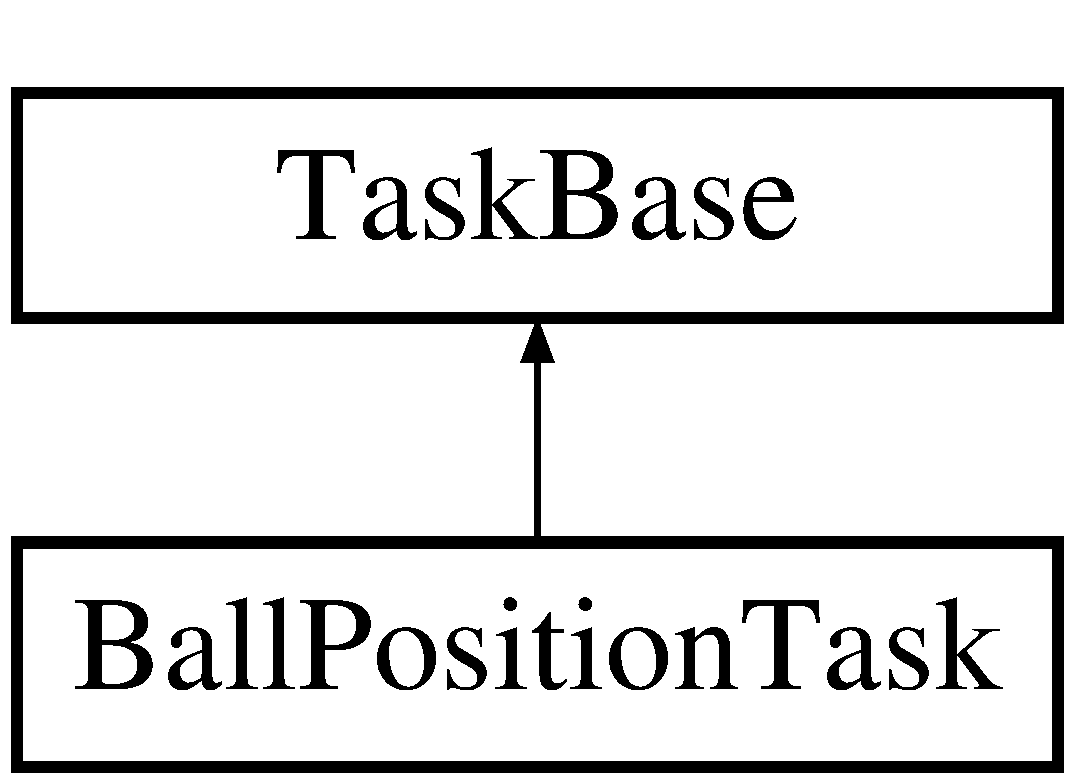
\includegraphics[height=2.000000cm]{class_ball_position_task}
\end{center}
\end{figure}
\subsection*{Public Member Functions}
\begin{DoxyCompactItemize}
\item 
\mbox{\hyperlink{class_ball_position_task_a4c6a431cab2bb0ed34445bfd79ba7dd5}{Ball\+Position\+Task}} (const char $\ast$a\+\_\+name, unsigned port\+B\+A\+S\+E\+\_\+\+T\+Y\+PE a\+\_\+priority, size\+\_\+t a\+\_\+stack\+\_\+size, \mbox{\hyperlink{classemstream}{emstream}} $\ast$p\+\_\+ser\+\_\+dev)
\begin{DoxyCompactList}\small\item\em Construct a Ball\+Position task. \end{DoxyCompactList}\item 
void \mbox{\hyperlink{class_ball_position_task_aa48c00fc26b05fe4f3c0cc8eed70fce4}{run}} (void)
\begin{DoxyCompactList}\small\item\em The run method of the Ball\+Position task that is repeatedly called by the R\+T\+OS scheduler. \end{DoxyCompactList}\end{DoxyCompactItemize}
\subsection*{Additional Inherited Members}


\subsection{Detailed Description}
Implements a task to determine the ball position. 

This class is an extension of {\ttfamily \mbox{\hyperlink{class_task_base}{Task\+Base}}}. The purpose of the class is to determine the physical states of the ball. 

\subsection{Constructor \& Destructor Documentation}
\mbox{\Hypertarget{class_ball_position_task_a4c6a431cab2bb0ed34445bfd79ba7dd5}\label{class_ball_position_task_a4c6a431cab2bb0ed34445bfd79ba7dd5}} 
\index{Ball\+Position\+Task@{Ball\+Position\+Task}!Ball\+Position\+Task@{Ball\+Position\+Task}}
\index{Ball\+Position\+Task@{Ball\+Position\+Task}!Ball\+Position\+Task@{Ball\+Position\+Task}}
\subsubsection{\texorpdfstring{Ball\+Position\+Task()}{BallPositionTask()}}
{\footnotesize\ttfamily Ball\+Position\+Task\+::\+Ball\+Position\+Task (\begin{DoxyParamCaption}\item[{const char $\ast$}]{a\+\_\+name,  }\item[{unsigned port\+B\+A\+S\+E\+\_\+\+T\+Y\+PE}]{a\+\_\+priority,  }\item[{size\+\_\+t}]{a\+\_\+stack\+\_\+size,  }\item[{\mbox{\hyperlink{classemstream}{emstream}} $\ast$}]{p\+\_\+ser\+\_\+dev }\end{DoxyParamCaption})}



Construct a Ball\+Position task. 

Constructor which creates and initializes a Ball\+Position task object.

This constructor sets up the task name, priority, stack size, and serial stream. 
\begin{DoxyParams}{Parameters}
{\em a\+\_\+name} & A character string which will be the name of this task \\
\hline
{\em a\+\_\+priority} & The priority at which this task will initially run (default\+: 0) \\
\hline
{\em a\+\_\+stack\+\_\+size} & The size of this task\textquotesingle{}s stack in bytes (default\+: {\ttfamily config\+M\+I\+N\+I\+M\+A\+L\+\_\+\+S\+T\+A\+C\+K\+\_\+\+S\+I\+ZE}) \\
\hline
{\em p\+\_\+ser\+\_\+dev} & Pointer to a serial device (port, radio, SD card, etc.) which can be used by this task to communicate (default\+: N\+U\+LL)\\
\hline
\end{DoxyParams}
This constructor creates a Free\+R\+T\+OS task with the given task run function, name, priority, and stack size. Its purpose is to determine the ball position and velocity from the sensor measurements and update the appropriate shared variables. 
\begin{DoxyParams}{Parameters}
{\em a\+\_\+name} & A character string which will be the name of this task \\
\hline
{\em a\+\_\+priority} & The priority at which this task will initially run (default\+: 0) \\
\hline
{\em a\+\_\+stack\+\_\+size} & The size of this task\textquotesingle{}s stack in bytes (default\+: {\ttfamily config\+M\+I\+N\+I\+M\+A\+L\+\_\+\+S\+T\+A\+C\+K\+\_\+\+S\+I\+ZE}) \\
\hline
{\em p\+\_\+ser\+\_\+dev} & Pointer to a serial device (port, radio, SD card, etc.) which can be used by this task to communicate (default\+: N\+U\+LL) \\
\hline
\end{DoxyParams}


\subsection{Member Function Documentation}
\mbox{\Hypertarget{class_ball_position_task_aa48c00fc26b05fe4f3c0cc8eed70fce4}\label{class_ball_position_task_aa48c00fc26b05fe4f3c0cc8eed70fce4}} 
\index{Ball\+Position\+Task@{Ball\+Position\+Task}!run@{run}}
\index{run@{run}!Ball\+Position\+Task@{Ball\+Position\+Task}}
\subsubsection{\texorpdfstring{run()}{run()}}
{\footnotesize\ttfamily void Ball\+Position\+Task\+::run (\begin{DoxyParamCaption}\item[{void}]{ }\end{DoxyParamCaption})\hspace{0.3cm}{\ttfamily [virtual]}}



The run method of the Ball\+Position task that is repeatedly called by the R\+T\+OS scheduler. 

The {\ttfamily \mbox{\hyperlink{class_ball_position_task_aa48c00fc26b05fe4f3c0cc8eed70fce4}{run()}}} function for the Ball\+Position task.

This method is called by the R\+T\+OS scheduler. The function converts the linear potentiometer measurements to ball position in m and ball velocity in m/s. Shared variables are updated after the calculations are performed. 

Implements \mbox{\hyperlink{class_task_base_adcf6036ad9c860051ccf392ba5e7dbbc}{Task\+Base}}.



The documentation for this class was generated from the following files\+:\begin{DoxyCompactItemize}
\item 
Doxygen\+Files/\mbox{\hyperlink{_ball_position_task_8h}{Ball\+Position\+Task.\+h}}\item 
Doxygen\+Files/Ball\+Position\+Task.\+cpp\end{DoxyCompactItemize}

\hypertarget{class_base_share}{}\section{Base\+Share Class Reference}
\label{class_base_share}\index{Base\+Share@{Base\+Share}}


Base class for classes that share data in a thread-\/safe manner between tasks.  




{\ttfamily \#include $<$baseshare.\+h$>$}

Inheritance diagram for Base\+Share\+:\begin{figure}[H]
\begin{center}
\leavevmode
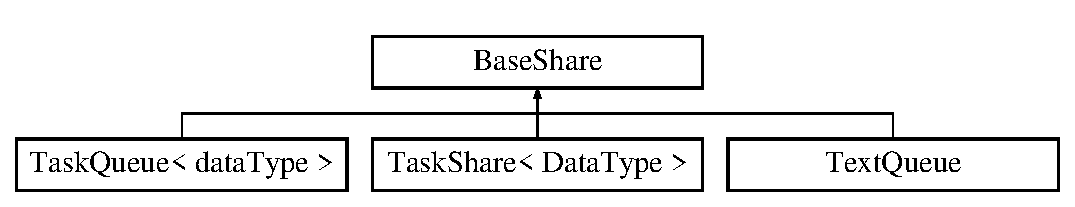
\includegraphics[height=2.000000cm]{class_base_share}
\end{center}
\end{figure}
\subsection*{Public Member Functions}
\begin{DoxyCompactItemize}
\item 
\mbox{\hyperlink{class_base_share_a9b0cfde3e2ee1869a507e7b8552ccf37}{Base\+Share}} (const char $\ast$p\+\_\+name)
\begin{DoxyCompactList}\small\item\em Construct a base shared data item. \end{DoxyCompactList}\item 
virtual void \mbox{\hyperlink{class_base_share_a81ef685c8c1897ee316e853103e9941a}{print\+\_\+in\+\_\+list}} (\mbox{\hyperlink{classemstream}{emstream}} $\ast$p\+\_\+ser\+\_\+dev)=0
\begin{DoxyCompactList}\small\item\em Construct a base shared data item. \end{DoxyCompactList}\item 
void \mbox{\hyperlink{class_base_share_a0112f588e48414498d6d2f12db7b347f}{print\+\_\+all\+\_\+shares}} (\mbox{\hyperlink{classemstream}{emstream}} $\ast$p\+\_\+ser\+\_\+dev)
\begin{DoxyCompactList}\small\item\em Start the printout showing the status of all shared data items. \end{DoxyCompactList}\end{DoxyCompactItemize}
\subsection*{Protected Attributes}
\begin{DoxyCompactItemize}
\item 
\mbox{\hyperlink{classemstream}{emstream}} $\ast$ \mbox{\hyperlink{class_base_share_af9176a9e2d467ccc1fd05f84bce4f74a}{p\+\_\+serial}}
\begin{DoxyCompactList}\small\item\em Pointer to a serial output device used for debugging. \end{DoxyCompactList}\item 
char $\ast$ \mbox{\hyperlink{class_base_share_a3da759fb6f803ddb8e3883435d91d29a}{name}}
\begin{DoxyCompactList}\small\item\em The name of the shared item. \end{DoxyCompactList}\item 
\mbox{\hyperlink{class_base_share}{Base\+Share}} $\ast$ \mbox{\hyperlink{class_base_share_a8077022ea40c4ba44a6ff07ab24cac83}{p\+\_\+next}}
\begin{DoxyCompactList}\small\item\em Pointer to the next item in the linked list of shares. \end{DoxyCompactList}\end{DoxyCompactItemize}
\subsection*{Static Protected Attributes}
\begin{DoxyCompactItemize}
\item 
static \mbox{\hyperlink{class_base_share}{Base\+Share}} $\ast$ \mbox{\hyperlink{class_base_share_a0657d8a02509e79c3bb418aaa9cce33c}{p\+\_\+newest}} = N\+U\+LL
\begin{DoxyCompactList}\small\item\em Pointer to the most recently created shared data item. \end{DoxyCompactList}\end{DoxyCompactItemize}


\subsection{Detailed Description}
Base class for classes that share data in a thread-\/safe manner between tasks. 

This is a base class for classes which share data between tasks without the risk of data corruption associated with global variables. Queues and task shares are two examples of such shared data classes. 

\subsection{Constructor \& Destructor Documentation}
\mbox{\Hypertarget{class_base_share_a9b0cfde3e2ee1869a507e7b8552ccf37}\label{class_base_share_a9b0cfde3e2ee1869a507e7b8552ccf37}} 
\index{Base\+Share@{Base\+Share}!Base\+Share@{Base\+Share}}
\index{Base\+Share@{Base\+Share}!Base\+Share@{Base\+Share}}
\subsubsection{\texorpdfstring{Base\+Share()}{BaseShare()}}
{\footnotesize\ttfamily Base\+Share\+::\+Base\+Share (\begin{DoxyParamCaption}\item[{const char $\ast$}]{p\+\_\+name = {\ttfamily NULL} }\end{DoxyParamCaption})}



Construct a base shared data item. 

This default constructor saves the name of the shared data item. It is not to be called by application code (nobody has any reason to create a base class object which can\textquotesingle{}t do anything!) but instead by the constructors of descendent classes. 
\begin{DoxyParams}{Parameters}
{\em p\+\_\+name} & The name for the shared data item, in a character string \\
\hline
\end{DoxyParams}


\subsection{Member Function Documentation}
\mbox{\Hypertarget{class_base_share_a0112f588e48414498d6d2f12db7b347f}\label{class_base_share_a0112f588e48414498d6d2f12db7b347f}} 
\index{Base\+Share@{Base\+Share}!print\+\_\+all\+\_\+shares@{print\+\_\+all\+\_\+shares}}
\index{print\+\_\+all\+\_\+shares@{print\+\_\+all\+\_\+shares}!Base\+Share@{Base\+Share}}
\subsubsection{\texorpdfstring{print\+\_\+all\+\_\+shares()}{print\_all\_shares()}}
{\footnotesize\ttfamily void Base\+Share\+::print\+\_\+all\+\_\+shares (\begin{DoxyParamCaption}\item[{\mbox{\hyperlink{classemstream}{emstream}} $\ast$}]{p\+\_\+ser\+\_\+dev }\end{DoxyParamCaption})\hspace{0.3cm}{\ttfamily [inline]}}



Start the printout showing the status of all shared data items. 

This method begins printing out the status of all items in the system\textquotesingle{}s linked list of shared data items (queues, task shares, and so on). The most recently created share\textquotesingle{}s status is printed first, followed by the status of other shares in reverse order of creation. \mbox{\Hypertarget{class_base_share_a81ef685c8c1897ee316e853103e9941a}\label{class_base_share_a81ef685c8c1897ee316e853103e9941a}} 
\index{Base\+Share@{Base\+Share}!print\+\_\+in\+\_\+list@{print\+\_\+in\+\_\+list}}
\index{print\+\_\+in\+\_\+list@{print\+\_\+in\+\_\+list}!Base\+Share@{Base\+Share}}
\subsubsection{\texorpdfstring{print\+\_\+in\+\_\+list()}{print\_in\_list()}}
{\footnotesize\ttfamily virtual void Base\+Share\+::print\+\_\+in\+\_\+list (\begin{DoxyParamCaption}\item[{\mbox{\hyperlink{classemstream}{emstream}} $\ast$}]{p\+\_\+ser\+\_\+dev }\end{DoxyParamCaption})\hspace{0.3cm}{\ttfamily [pure virtual]}}



Construct a base shared data item. 

Make a printout showing the condition of this shared data item, such as the value of a shared variable or how full a queue\textquotesingle{}s buffer is. This method must be overridden in each descendent class with a method that actually {\itshape does} something. 
\begin{DoxyParams}{Parameters}
{\em p\+\_\+ser\+\_\+dev} & Pointer to a serial device on which to print things \\
\hline
\end{DoxyParams}


Implemented in \mbox{\hyperlink{class_task_queue_ad5ccb9c99ca4f43304d408d915314d71}{Task\+Queue$<$ data\+Type $>$}}, \mbox{\hyperlink{class_text_queue_aeef41a1bc3486d98fb31cba9ce539d0d}{Text\+Queue}}, and \mbox{\hyperlink{class_task_share_a08835a91ed7ccd847cefe6ff72fe22e6}{Task\+Share$<$ Data\+Type $>$}}.



\subsection{Member Data Documentation}
\mbox{\Hypertarget{class_base_share_a3da759fb6f803ddb8e3883435d91d29a}\label{class_base_share_a3da759fb6f803ddb8e3883435d91d29a}} 
\index{Base\+Share@{Base\+Share}!name@{name}}
\index{name@{name}!Base\+Share@{Base\+Share}}
\subsubsection{\texorpdfstring{name}{name}}
{\footnotesize\ttfamily char$\ast$ Base\+Share\+::name\hspace{0.3cm}{\ttfamily [protected]}}



The name of the shared item. 

This string holds the shared item\textquotesingle{}s name. The name is only used for identification on debugging printouts or logs. \mbox{\Hypertarget{class_base_share_a0657d8a02509e79c3bb418aaa9cce33c}\label{class_base_share_a0657d8a02509e79c3bb418aaa9cce33c}} 
\index{Base\+Share@{Base\+Share}!p\+\_\+newest@{p\+\_\+newest}}
\index{p\+\_\+newest@{p\+\_\+newest}!Base\+Share@{Base\+Share}}
\subsubsection{\texorpdfstring{p\+\_\+newest}{p\_newest}}
{\footnotesize\ttfamily \mbox{\hyperlink{class_base_share}{Base\+Share}} $\ast$ Base\+Share\+::p\+\_\+newest = N\+U\+LL\hspace{0.3cm}{\ttfamily [static]}, {\ttfamily [protected]}}



Pointer to the most recently created shared data item. 

This {\ttfamily static} variable, one copy of which is shared by all shared data items, is a pointer to the most recently created one. It is used as the beginning of a linked list of all shared data items in the system. \mbox{\Hypertarget{class_base_share_a8077022ea40c4ba44a6ff07ab24cac83}\label{class_base_share_a8077022ea40c4ba44a6ff07ab24cac83}} 
\index{Base\+Share@{Base\+Share}!p\+\_\+next@{p\+\_\+next}}
\index{p\+\_\+next@{p\+\_\+next}!Base\+Share@{Base\+Share}}
\subsubsection{\texorpdfstring{p\+\_\+next}{p\_next}}
{\footnotesize\ttfamily \mbox{\hyperlink{class_base_share}{Base\+Share}}$\ast$ Base\+Share\+::p\+\_\+next\hspace{0.3cm}{\ttfamily [protected]}}



Pointer to the next item in the linked list of shares. 

This pointer points to the next item in the system\textquotesingle{}s list of shared data items (shares, queues, {\itshape etc}.) If this share is the most recently created one, the pointer will be {\ttfamily N\+U\+LL}. The list goes backwards; the next item is the previously created one. \mbox{\Hypertarget{class_base_share_af9176a9e2d467ccc1fd05f84bce4f74a}\label{class_base_share_af9176a9e2d467ccc1fd05f84bce4f74a}} 
\index{Base\+Share@{Base\+Share}!p\+\_\+serial@{p\+\_\+serial}}
\index{p\+\_\+serial@{p\+\_\+serial}!Base\+Share@{Base\+Share}}
\subsubsection{\texorpdfstring{p\+\_\+serial}{p\_serial}}
{\footnotesize\ttfamily \mbox{\hyperlink{classemstream}{emstream}}$\ast$ Base\+Share\+::p\+\_\+serial\hspace{0.3cm}{\ttfamily [protected]}}



Pointer to a serial output device used for debugging. 

This pointer can point to a serial output device or port which will be used for various diagnostic printouts or logging. 

The documentation for this class was generated from the following files\+:\begin{DoxyCompactItemize}
\item 
Doxygen\+Files/\mbox{\hyperlink{baseshare_8h}{baseshare.\+h}}\item 
Doxygen\+Files/baseshare.\+cpp\end{DoxyCompactItemize}

\hypertarget{class_communication_task}{}\section{Communication\+Task Class Reference}
\label{class_communication_task}\index{Communication\+Task@{Communication\+Task}}


Implements a task to communicate with serial devices.  


Inheritance diagram for Communication\+Task\+:\begin{figure}[H]
\begin{center}
\leavevmode
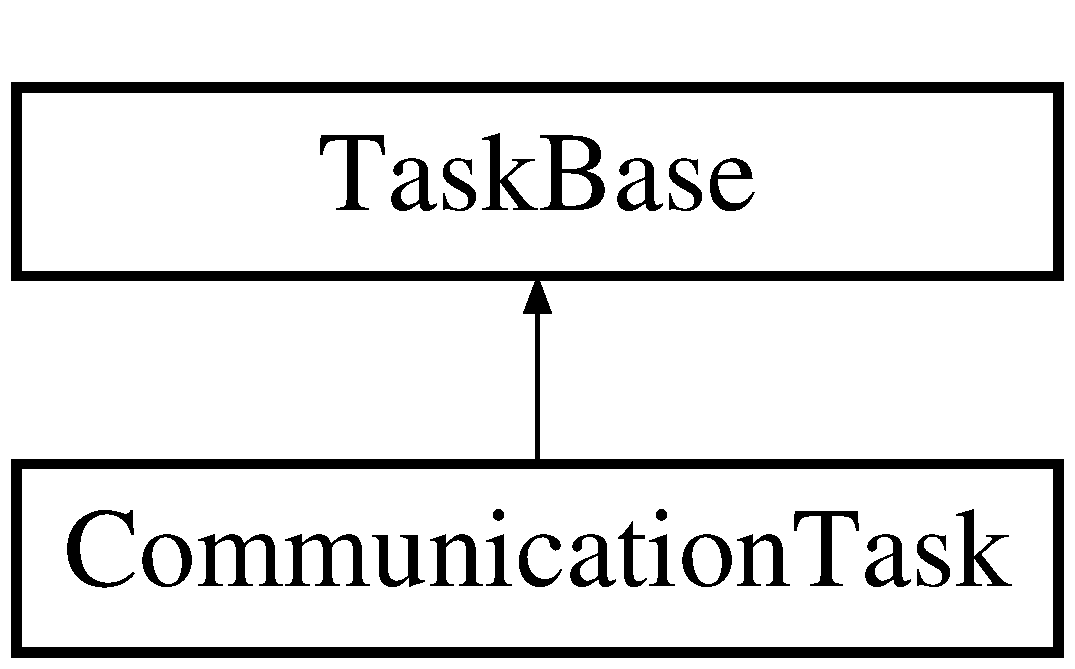
\includegraphics[height=2.000000cm]{class_communication_task}
\end{center}
\end{figure}
\subsection*{Public Member Functions}
\begin{DoxyCompactItemize}
\item 
\mbox{\hyperlink{class_communication_task_ac76f495e2350156d1faaa1a3198fe80f}{Communication\+Task}} (const char $\ast$a\+\_\+name, unsigned port\+B\+A\+S\+E\+\_\+\+T\+Y\+PE a\+\_\+priority, size\+\_\+t a\+\_\+stack\+\_\+size, \mbox{\hyperlink{classemstream}{emstream}} $\ast$p\+\_\+ser\+\_\+dev)
\begin{DoxyCompactList}\small\item\em Construct a Communication task. \end{DoxyCompactList}\item 
void \mbox{\hyperlink{class_communication_task_a33c23712d6b6952d3e7fb180bab34a83}{run}} (void)
\begin{DoxyCompactList}\small\item\em The run method of the Communication task that is repeatedly called by the R\+T\+OS scheduler. \end{DoxyCompactList}\end{DoxyCompactItemize}
\subsection*{Additional Inherited Members}


\subsection{Detailed Description}
Implements a task to communicate with serial devices. 

This class is an extension of {\ttfamily \mbox{\hyperlink{class_task_base}{Task\+Base}}}. The purpose of the class is to handle S\+T\+M32 hardware and communicate with external serial devices. 

\subsection{Constructor \& Destructor Documentation}
\mbox{\Hypertarget{class_communication_task_ac76f495e2350156d1faaa1a3198fe80f}\label{class_communication_task_ac76f495e2350156d1faaa1a3198fe80f}} 
\index{Communication\+Task@{Communication\+Task}!Communication\+Task@{Communication\+Task}}
\index{Communication\+Task@{Communication\+Task}!Communication\+Task@{Communication\+Task}}
\subsubsection{\texorpdfstring{Communication\+Task()}{CommunicationTask()}}
{\footnotesize\ttfamily Communication\+Task\+::\+Communication\+Task (\begin{DoxyParamCaption}\item[{const char $\ast$}]{a\+\_\+name,  }\item[{unsigned port\+B\+A\+S\+E\+\_\+\+T\+Y\+PE}]{a\+\_\+priority,  }\item[{size\+\_\+t}]{a\+\_\+stack\+\_\+size,  }\item[{\mbox{\hyperlink{classemstream}{emstream}} $\ast$}]{p\+\_\+ser\+\_\+dev }\end{DoxyParamCaption})}



Construct a Communication task. 

Constructor which creates and initializes a Communication task object.

This constructor sets up the task name, priority, stack size, and serial stream. 
\begin{DoxyParams}{Parameters}
{\em a\+\_\+name} & A character string which will be the name of this task \\
\hline
{\em a\+\_\+priority} & The priority at which this task will initially run (default\+: 0) \\
\hline
{\em a\+\_\+stack\+\_\+size} & The size of this task\textquotesingle{}s stack in bytes (default\+: {\ttfamily config\+M\+I\+N\+I\+M\+A\+L\+\_\+\+S\+T\+A\+C\+K\+\_\+\+S\+I\+ZE}) \\
\hline
{\em p\+\_\+ser\+\_\+dev} & Pointer to a serial device (port, radio, SD card, etc.) which can be used by this task to communicate (default\+: N\+U\+LL)\\
\hline
\end{DoxyParams}
This constructor creates a Free\+R\+T\+OS task with the given task run function, name, priority, and stack size. Its purpose is to talk to external serial devices and interface with the S\+T\+M32 hardware. 
\begin{DoxyParams}{Parameters}
{\em a\+\_\+name} & A character string which will be the name of this task \\
\hline
{\em a\+\_\+priority} & The priority at which this task will initially run (default\+: 0) \\
\hline
{\em a\+\_\+stack\+\_\+size} & The size of this task\textquotesingle{}s stack in bytes (default\+: {\ttfamily config\+M\+I\+N\+I\+M\+A\+L\+\_\+\+S\+T\+A\+C\+K\+\_\+\+S\+I\+ZE}) \\
\hline
{\em p\+\_\+ser\+\_\+dev} & Pointer to a serial device (port, radio, SD card, etc.) which can be used by this task to communicate (default\+: N\+U\+LL) \\
\hline
\end{DoxyParams}


\subsection{Member Function Documentation}
\mbox{\Hypertarget{class_communication_task_a33c23712d6b6952d3e7fb180bab34a83}\label{class_communication_task_a33c23712d6b6952d3e7fb180bab34a83}} 
\index{Communication\+Task@{Communication\+Task}!run@{run}}
\index{run@{run}!Communication\+Task@{Communication\+Task}}
\subsubsection{\texorpdfstring{run()}{run()}}
{\footnotesize\ttfamily void Communication\+Task\+::run (\begin{DoxyParamCaption}\item[{void}]{ }\end{DoxyParamCaption})\hspace{0.3cm}{\ttfamily [virtual]}}



The run method of the Communication task that is repeatedly called by the R\+T\+OS scheduler. 

The {\ttfamily \mbox{\hyperlink{class_communication_task_a33c23712d6b6952d3e7fb180bab34a83}{run()}}} function for the Communication task.

This method is called by the R\+T\+OS scheduler. The function sets the P\+WM duty cycle to the correct hardware pin, reads the A\+DC, reads the S\+PI serial bus (encoder) and prints the state variables to the external serial device over U\+S\+A\+RT. 

Implements \mbox{\hyperlink{class_task_base_adcf6036ad9c860051ccf392ba5e7dbbc}{Task\+Base}}.



The documentation for this class was generated from the following file\+:\begin{DoxyCompactItemize}
\item 
Doxygen\+Files/\mbox{\hyperlink{main_8cpp}{main.\+cpp}}\end{DoxyCompactItemize}

\hypertarget{class_controller_task}{}\section{Controller\+Task Class Reference}
\label{class_controller_task}\index{Controller\+Task@{Controller\+Task}}


Implements a task to control the system.  




{\ttfamily \#include $<$Controller\+Task.\+h$>$}

Inheritance diagram for Controller\+Task\+:\begin{figure}[H]
\begin{center}
\leavevmode
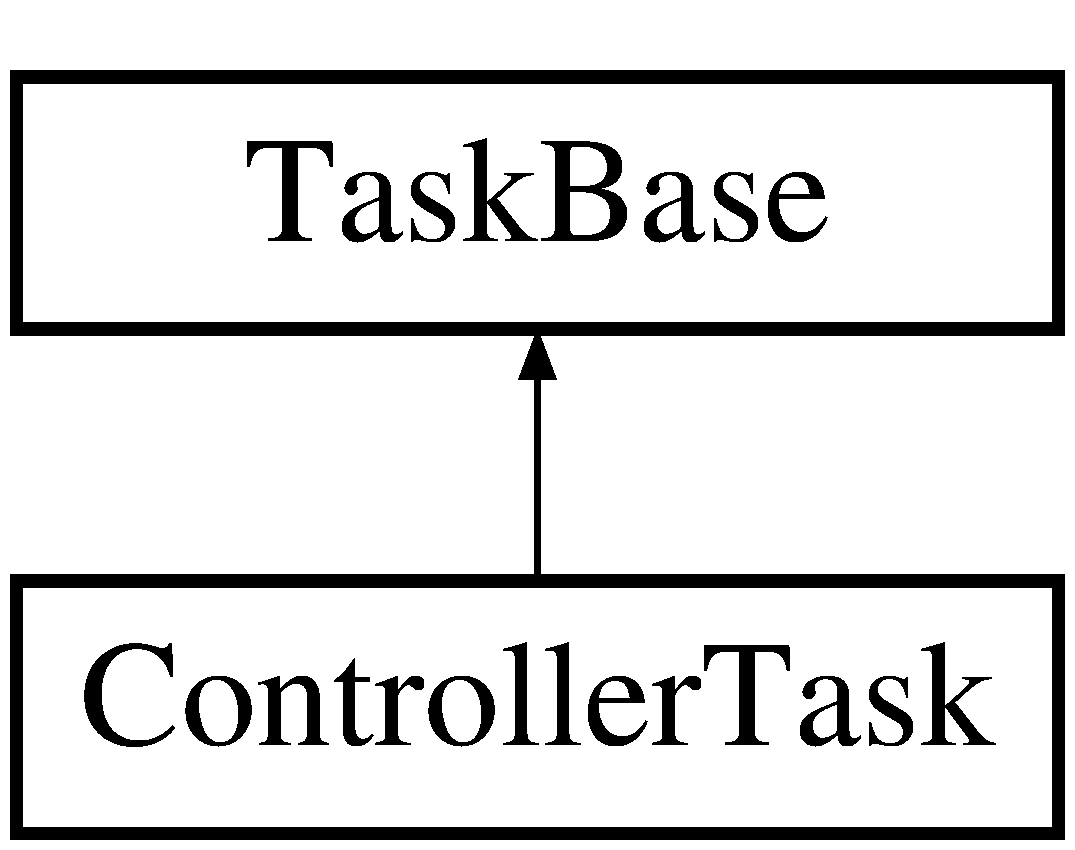
\includegraphics[height=2.000000cm]{class_controller_task}
\end{center}
\end{figure}
\subsection*{Public Member Functions}
\begin{DoxyCompactItemize}
\item 
\mbox{\hyperlink{class_controller_task_a2b2914fa356737e69e9ec1e3ffd3a8e3}{Controller\+Task}} (const char $\ast$a\+\_\+name, unsigned port\+B\+A\+S\+E\+\_\+\+T\+Y\+PE a\+\_\+priority, size\+\_\+t a\+\_\+stack\+\_\+size, \mbox{\hyperlink{classemstream}{emstream}} $\ast$p\+\_\+ser\+\_\+dev)
\begin{DoxyCompactList}\small\item\em Construct a Ball\+Position task. \end{DoxyCompactList}\item 
void \mbox{\hyperlink{class_controller_task_adb32c437ea51d258b986414ab48c6180}{run}} (void)
\begin{DoxyCompactList}\small\item\em The run method of the Controller task that is repeatedly called by the R\+T\+OS scheduler. \end{DoxyCompactList}\end{DoxyCompactItemize}
\subsection*{Additional Inherited Members}


\subsection{Detailed Description}
Implements a task to control the system. 

This class is an extension of {\ttfamily \mbox{\hyperlink{class_task_base}{Task\+Base}}}. The purpose of the class is to determine the voltage input to the motor in response to state feedback from the ball and beam sensor measurements. 

\subsection{Constructor \& Destructor Documentation}
\mbox{\Hypertarget{class_controller_task_a2b2914fa356737e69e9ec1e3ffd3a8e3}\label{class_controller_task_a2b2914fa356737e69e9ec1e3ffd3a8e3}} 
\index{Controller\+Task@{Controller\+Task}!Controller\+Task@{Controller\+Task}}
\index{Controller\+Task@{Controller\+Task}!Controller\+Task@{Controller\+Task}}
\subsubsection{\texorpdfstring{Controller\+Task()}{ControllerTask()}}
{\footnotesize\ttfamily Controller\+Task\+::\+Controller\+Task (\begin{DoxyParamCaption}\item[{const char $\ast$}]{a\+\_\+name,  }\item[{unsigned port\+B\+A\+S\+E\+\_\+\+T\+Y\+PE}]{a\+\_\+priority,  }\item[{size\+\_\+t}]{a\+\_\+stack\+\_\+size,  }\item[{\mbox{\hyperlink{classemstream}{emstream}} $\ast$}]{p\+\_\+ser\+\_\+dev }\end{DoxyParamCaption})}



Construct a Ball\+Position task. 

Constructor which creates and initializes a controller task object.

This constructor sets up the task name, priority, stack size, and serial stream. 
\begin{DoxyParams}{Parameters}
{\em a\+\_\+name} & A character string which will be the name of this task \\
\hline
{\em a\+\_\+priority} & The priority at which this task will initially run (default\+: 0) \\
\hline
{\em a\+\_\+stack\+\_\+size} & The size of this task\textquotesingle{}s stack in bytes (default\+: {\ttfamily config\+M\+I\+N\+I\+M\+A\+L\+\_\+\+S\+T\+A\+C\+K\+\_\+\+S\+I\+ZE}) \\
\hline
{\em p\+\_\+ser\+\_\+dev} & Pointer to a serial device (port, radio, SD card, etc.) which can be used by this task to communicate (default\+: N\+U\+LL)\\
\hline
\end{DoxyParams}
This constructor creates a Free\+R\+T\+OS task with the given task run function, name, priority, and stack size. Its purpose is to implement the state space control algorithm with established gains. 
\begin{DoxyParams}{Parameters}
{\em a\+\_\+name} & A character string which will be the name of this task \\
\hline
{\em a\+\_\+priority} & The priority at which this task will initially run (default\+: 0) \\
\hline
{\em a\+\_\+stack\+\_\+size} & The size of this task\textquotesingle{}s stack in bytes (default\+: {\ttfamily config\+M\+I\+N\+I\+M\+A\+L\+\_\+\+S\+T\+A\+C\+K\+\_\+\+S\+I\+ZE}) \\
\hline
{\em p\+\_\+ser\+\_\+dev} & Pointer to a serial device (port, radio, SD card, etc.) which can be used by this task to communicate (default\+: N\+U\+LL) \\
\hline
\end{DoxyParams}


\subsection{Member Function Documentation}
\mbox{\Hypertarget{class_controller_task_adb32c437ea51d258b986414ab48c6180}\label{class_controller_task_adb32c437ea51d258b986414ab48c6180}} 
\index{Controller\+Task@{Controller\+Task}!run@{run}}
\index{run@{run}!Controller\+Task@{Controller\+Task}}
\subsubsection{\texorpdfstring{run()}{run()}}
{\footnotesize\ttfamily void Controller\+Task\+::run (\begin{DoxyParamCaption}\item[{void}]{ }\end{DoxyParamCaption})\hspace{0.3cm}{\ttfamily [virtual]}}



The run method of the Controller task that is repeatedly called by the R\+T\+OS scheduler. 

The {\ttfamily \mbox{\hyperlink{class_controller_task_adb32c437ea51d258b986414ab48c6180}{run()}}} function for the Controller task.

This method is called by the R\+T\+OS scheduler. The function reads the system system states and establishes the required P\+WM signal to send to the motor. N\+O\+TE\+: The control algorithm is F\+U\+LL S\+T\+A\+TE F\+E\+E\+D\+B\+A\+CK 

Implements \mbox{\hyperlink{class_task_base_adcf6036ad9c860051ccf392ba5e7dbbc}{Task\+Base}}.



The documentation for this class was generated from the following files\+:\begin{DoxyCompactItemize}
\item 
Doxygen\+Files/\mbox{\hyperlink{_controller_task_8h}{Controller\+Task.\+h}}\item 
Doxygen\+Files/Controller\+Task.\+cpp\end{DoxyCompactItemize}

\hypertarget{structdevice_params__t}{}\section{device\+Params\+\_\+t Struct Reference}
\label{structdevice_params__t}\index{device\+Params\+\_\+t@{device\+Params\+\_\+t}}


Device Parameters Structure Type.  




{\ttfamily \#include $<$l6206.\+h$>$}

\subsection*{Public Attributes}
\begin{DoxyCompactItemize}
\item 
\mbox{\Hypertarget{structdevice_params__t_ab85a421e14122b7be3738c9d8298af05}\label{structdevice_params__t_ab85a421e14122b7be3738c9d8298af05}} 
\mbox{\hyperlink{group___dual___full___bridge___configuration_gab5810188b32c0f4c04abcbf058f09722}{dual\+Full\+Bridge\+Config\+\_\+t}} \mbox{\hyperlink{structdevice_params__t_ab85a421e14122b7be3738c9d8298af05}{config}}
\begin{DoxyCompactList}\small\item\em Dual full bridge configuration. \end{DoxyCompactList}\item 
\mbox{\Hypertarget{structdevice_params__t_a42e0cba17c7c8325057e6f82f34e3161}\label{structdevice_params__t_a42e0cba17c7c8325057e6f82f34e3161}} 
uint32\+\_\+t \mbox{\hyperlink{structdevice_params__t_a42e0cba17c7c8325057e6f82f34e3161}{pwm\+Freq}} \mbox{[}\mbox{\hyperlink{group___l6206___exported___constants_ga672b88d2cc08d7e4216e226f966c862b}{L6206\+\_\+\+N\+B\+\_\+\+M\+A\+X\+\_\+\+B\+R\+I\+D\+G\+E\+\_\+\+I\+N\+P\+UT}}\mbox{]}
\begin{DoxyCompactList}\small\item\em Pwm frequency of the bridge input. \end{DoxyCompactList}\item 
\mbox{\Hypertarget{structdevice_params__t_aa77caca6f867297f3cf05c1867be0a9f}\label{structdevice_params__t_aa77caca6f867297f3cf05c1867be0a9f}} 
uint16\+\_\+t \mbox{\hyperlink{structdevice_params__t_aa77caca6f867297f3cf05c1867be0a9f}{speed}} \mbox{[}\mbox{\hyperlink{group___l6206___exported___constants_ga64b1ce7748d44eb6f6973dfe8c7fd196}{L6206\+\_\+\+N\+B\+\_\+\+M\+A\+X\+\_\+\+M\+O\+T\+O\+RS}}\mbox{]}
\begin{DoxyCompactList}\small\item\em Speed\% (from 0 to 100) of the corresponding motor. \end{DoxyCompactList}\item 
\mbox{\Hypertarget{structdevice_params__t_ad7a3b05d9d1885313de00fd680de5e0a}\label{structdevice_params__t_ad7a3b05d9d1885313de00fd680de5e0a}} 
\mbox{\hyperlink{group___device___direction___options_ga4eaf4196e4d11d552f58f3fab218a8c7}{motor\+Dir\+\_\+t}} \mbox{\hyperlink{structdevice_params__t_ad7a3b05d9d1885313de00fd680de5e0a}{direction}} \mbox{[}\mbox{\hyperlink{group___l6206___exported___constants_ga64b1ce7748d44eb6f6973dfe8c7fd196}{L6206\+\_\+\+N\+B\+\_\+\+M\+A\+X\+\_\+\+M\+O\+T\+O\+RS}}\mbox{]}
\begin{DoxyCompactList}\small\item\em F\+O\+R\+W\+A\+RD or B\+A\+C\+K\+W\+A\+RD direction of the motors. \end{DoxyCompactList}\item 
\mbox{\Hypertarget{structdevice_params__t_af776d12dbf2213478b02d604fac81a89}\label{structdevice_params__t_af776d12dbf2213478b02d604fac81a89}} 
\mbox{\hyperlink{group___device___states_ga9ba865be7705688e94f95a410e917a07}{motor\+State\+\_\+t}} \mbox{\hyperlink{structdevice_params__t_af776d12dbf2213478b02d604fac81a89}{motion\+State}} \mbox{[}\mbox{\hyperlink{group___l6206___exported___constants_ga64b1ce7748d44eb6f6973dfe8c7fd196}{L6206\+\_\+\+N\+B\+\_\+\+M\+A\+X\+\_\+\+M\+O\+T\+O\+RS}}\mbox{]}
\begin{DoxyCompactList}\small\item\em Current State of the motors. \end{DoxyCompactList}\item 
\mbox{\Hypertarget{structdevice_params__t_a7d064cc0096019e667d28c80c31be7a8}\label{structdevice_params__t_a7d064cc0096019e667d28c80c31be7a8}} 
\mbox{\hyperlink{group___motor___boolean___type_ga0ecf26b576b9a54eca656b9be7ba6a06}{bool}} \mbox{\hyperlink{structdevice_params__t_a7d064cc0096019e667d28c80c31be7a8}{bridge\+Enabled}} \mbox{[}\mbox{\hyperlink{group___l6206___exported___constants_gae72db6f074defd956d309151334f448d}{L6206\+\_\+\+N\+B\+\_\+\+M\+A\+X\+\_\+\+B\+R\+I\+D\+G\+ES}}\mbox{]}
\begin{DoxyCompactList}\small\item\em Current State of the bridges. \end{DoxyCompactList}\end{DoxyCompactItemize}


\subsection{Detailed Description}
Device Parameters Structure Type. 

The documentation for this struct was generated from the following file\+:\begin{DoxyCompactItemize}
\item 
Doxygen\+Files/\mbox{\hyperlink{l6206_8h}{l6206.\+h}}\end{DoxyCompactItemize}

\hypertarget{classemstream}{}\section{emstream Class Reference}
\label{classemstream}\index{emstream@{emstream}}


Base class for serial devices which print using a {\ttfamily $<$$<$} operator.  




{\ttfamily \#include $<$emstream.\+h$>$}

Inheritance diagram for emstream\+:\begin{figure}[H]
\begin{center}
\leavevmode
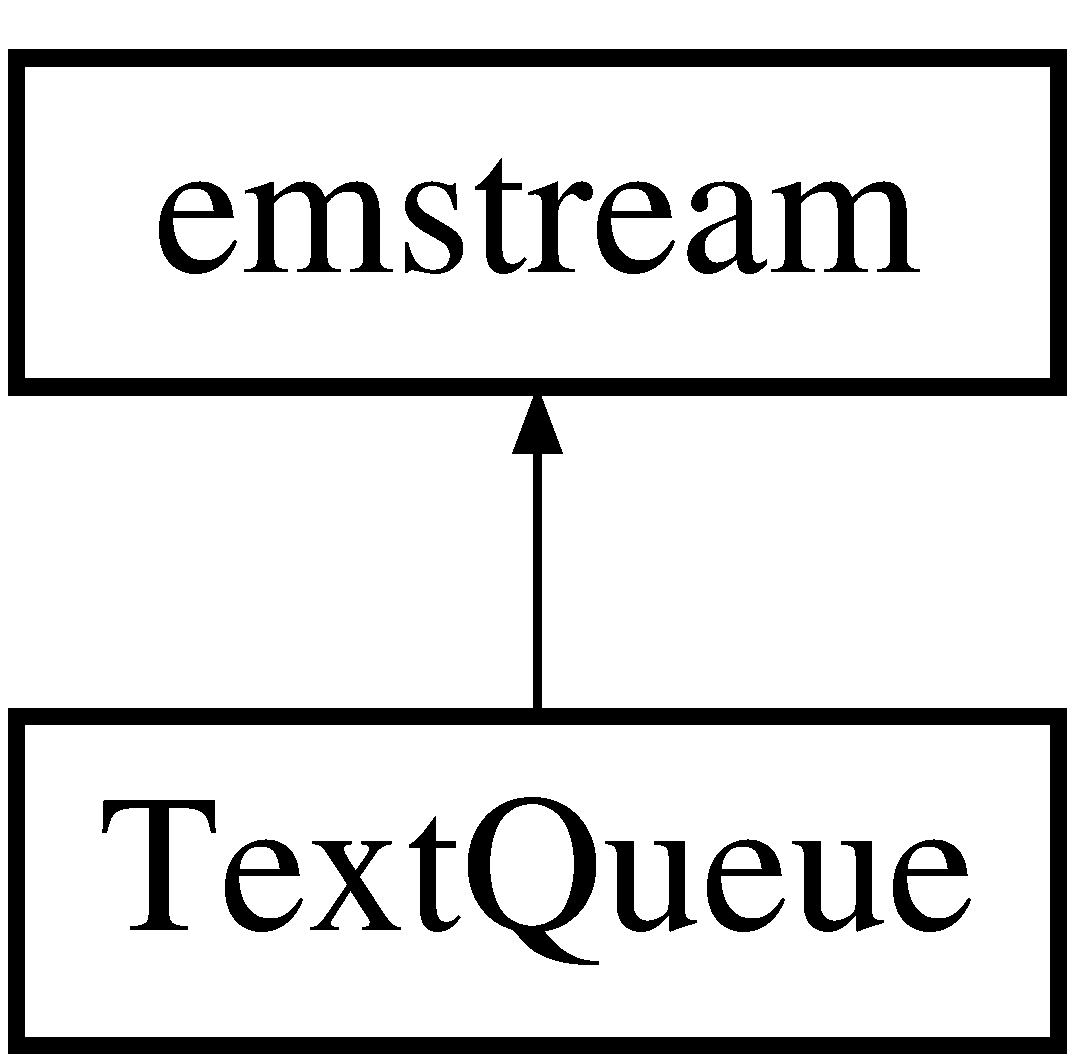
\includegraphics[height=2.000000cm]{classemstream}
\end{center}
\end{figure}
\subsection*{Public Member Functions}
\begin{DoxyCompactItemize}
\item 
\mbox{\hyperlink{classemstream_ad19a1ff84926b5fd5feac71fc2f7fb51}{emstream}} (void)
\begin{DoxyCompactList}\small\item\em Create a base text stream object. \end{DoxyCompactList}\item 
virtual \mbox{\hyperlink{group___motor___boolean___type_ga0ecf26b576b9a54eca656b9be7ba6a06}{bool}} \mbox{\hyperlink{classemstream_a28149c19ad19d10d89ca8dd3d3803b1a}{ready\+\_\+to\+\_\+send}} (void)
\begin{DoxyCompactList}\small\item\em Check if a serial device is ready to transmit characters. \end{DoxyCompactList}\item 
virtual void \mbox{\hyperlink{classemstream_aa4dffc9aa58f601cc4153b4cbe65d757}{putchar}} (char a\+\_\+char)=0
\begin{DoxyCompactList}\small\item\em Base method for sending one character. \end{DoxyCompactList}\item 
void \mbox{\hyperlink{classemstream_a1ad530cbebe6c54640c1db8c1b9afda2}{puts}} (const char $\ast$)
\begin{DoxyCompactList}\small\item\em Write a character string to a serial device. \end{DoxyCompactList}\item 
virtual \mbox{\hyperlink{group___motor___boolean___type_ga0ecf26b576b9a54eca656b9be7ba6a06}{bool}} \mbox{\hyperlink{classemstream_a64494c4283e4750d29d93df245045d56}{check\+\_\+for\+\_\+char}} (void)
\begin{DoxyCompactList}\small\item\em Check if a character is ready to read from a serial device. \end{DoxyCompactList}\item 
\mbox{\Hypertarget{classemstream_af514146b9ca7d4091a688b413b422d50}\label{classemstream_af514146b9ca7d4091a688b413b422d50}} 
virtual char {\bfseries peek} (void)=0
\item 
virtual char \mbox{\hyperlink{classemstream_a41f0814540d5baa7312310c59077a248}{getchar}} (void)
\begin{DoxyCompactList}\small\item\em Get a character from a serial device. \end{DoxyCompactList}\item 
virtual void \mbox{\hyperlink{classemstream_a3ef6ddf641176d416f9ae6a5c4cfc067}{transmit\+\_\+now}} (void)
\begin{DoxyCompactList}\small\item\em Cause a transmitter to send buffered characters immediately. \end{DoxyCompactList}\item 
virtual void \mbox{\hyperlink{classemstream_a8dcff85fe80c250b20b5da78b1799ed5}{clear\+\_\+screen}} (void)
\begin{DoxyCompactList}\small\item\em Clear a display screen. \end{DoxyCompactList}\item 
\mbox{\hyperlink{classemstream}{emstream}} \& \mbox{\hyperlink{classemstream_a180fa065e30c2e97e957a97b70eb8eb4}{operator$<$$<$}} (\mbox{\hyperlink{group___motor___boolean___type_ga0ecf26b576b9a54eca656b9be7ba6a06}{bool}})
\begin{DoxyCompactList}\small\item\em Write unsigned an 8-\/bit unsigned number to a serial device. \end{DoxyCompactList}\item 
\mbox{\hyperlink{classemstream}{emstream}} \& \mbox{\hyperlink{classemstream_ac570021b41b465fd0f98257a17316e7b}{operator$<$$<$}} (const char $\ast$p\+\_\+string)
\item 
\mbox{\hyperlink{classemstream}{emstream}} \& \mbox{\hyperlink{classemstream_a2125b913b6a300c4ac176af247ff5a53}{operator$<$$<$}} (char ch)
\item 
\mbox{\Hypertarget{classemstream_a28fcc39c98ff38302cba6b3eb98b66f0}\label{classemstream_a28fcc39c98ff38302cba6b3eb98b66f0}} 
\mbox{\hyperlink{classemstream}{emstream}} \& {\bfseries operator$<$$<$} (uint8\+\_\+t)
\item 
\mbox{\hyperlink{classemstream}{emstream}} \& \mbox{\hyperlink{classemstream_a8666557b0248286fd70a69d6e0106f4f}{operator$<$$<$}} (int8\+\_\+t)
\begin{DoxyCompactList}\small\item\em Write a signed 8-\/bit number to a serial device. \end{DoxyCompactList}\item 
\mbox{\hyperlink{classemstream}{emstream}} \& \mbox{\hyperlink{classemstream_aed40605be053b7cbae14201162028781}{operator$<$$<$}} (uint16\+\_\+t)
\begin{DoxyCompactList}\small\item\em Write unsigned 16-\/bit numbers to a serial device. \end{DoxyCompactList}\item 
\mbox{\hyperlink{classemstream}{emstream}} \& \mbox{\hyperlink{classemstream_a40243877b820b91c9798e99fd565f85f}{operator$<$$<$}} (int16\+\_\+t)
\begin{DoxyCompactList}\small\item\em Write a signed 16-\/bit number to a serial device. \end{DoxyCompactList}\item 
\mbox{\hyperlink{classemstream}{emstream}} \& \mbox{\hyperlink{classemstream_aa3915880211b615d4f889036683c53c3}{operator$<$$<$}} (uint32\+\_\+t)
\begin{DoxyCompactList}\small\item\em Write an unsigned 32-\/bit number to a serial device. \end{DoxyCompactList}\item 
\mbox{\hyperlink{classemstream}{emstream}} \& \mbox{\hyperlink{classemstream_abf54c92665eaecae12af886b4275ded3}{operator$<$$<$}} (int32\+\_\+t)
\begin{DoxyCompactList}\small\item\em Write a signed 32-\/bit number to a serial device. \end{DoxyCompactList}\item 
\mbox{\hyperlink{classemstream}{emstream}} \& \mbox{\hyperlink{classemstream_aad47341203535f0c3b8d34f63fa0723f}{operator$<$$<$}} (uint64\+\_\+t)
\begin{DoxyCompactList}\small\item\em Write an unsigned 64-\/bit number to a serial device. \end{DoxyCompactList}\item 
\mbox{\hyperlink{classemstream}{emstream}} \& \mbox{\hyperlink{classemstream_ad0b6eeba3130fb192413f43cfb1670fe}{operator$<$$<$}} (int64\+\_\+t)
\begin{DoxyCompactList}\small\item\em Write a signed 64-\/bit number to a serial device. \end{DoxyCompactList}\item 
\mbox{\hyperlink{classemstream}{emstream}} \& \mbox{\hyperlink{classemstream_a87d81e918bc1baa294ee9c9c3d056ea7}{operator$<$$<$}} (void $\ast$)
\begin{DoxyCompactList}\small\item\em Write a pointer to a serial device. \end{DoxyCompactList}\item 
\mbox{\hyperlink{classemstream}{emstream}} \& \mbox{\hyperlink{classemstream_ab0ea0ed8ea67a4182d526bdae23d4594}{operator$<$$<$}} (float)
\begin{DoxyCompactList}\small\item\em Write a single precision floating point number to a serial device. \end{DoxyCompactList}\item 
\mbox{\hyperlink{classemstream}{emstream}} \& \mbox{\hyperlink{classemstream_a14caec5bbf12dd25ae39c72a95bebf0b}{operator$<$$<$}} (double)
\item 
\mbox{\hyperlink{classemstream}{emstream}} \& \mbox{\hyperlink{classemstream_a10a043d75a8d229974282c0bac207dab}{operator$<$$<$}} (\mbox{\hyperlink{emstream_8h_a5582483c459c0f48e51d96478d5b3407}{ser\+\_\+manipulator}})
\begin{DoxyCompactList}\small\item\em Overloaded operator used to print things to a serial device. \end{DoxyCompactList}\item 
\mbox{\hyperlink{classemstream}{emstream}} \& \mbox{\hyperlink{classemstream_a67dc7f8341184dffa95daf0104406e17}{operator$>$$>$}} (char \&ch)
\begin{DoxyCompactList}\small\item\em Stream input operator which reads a single character. \end{DoxyCompactList}\item 
\mbox{\hyperlink{classemstream}{emstream}} \& \mbox{\hyperlink{classemstream_ab27cadcdfb7256a05c2474c954fd02b8}{operator$>$$>$}} (uint8\+\_\+t \&number)
\begin{DoxyCompactList}\small\item\em Read an 8-\/bit unsigned decimal integer from a serial device. \end{DoxyCompactList}\item 
\mbox{\hyperlink{classemstream}{emstream}} \& \mbox{\hyperlink{classemstream_a8dfe916d7db9331beaf5dc98b6c5b9ea}{operator$>$$>$}} (int8\+\_\+t \&number)
\begin{DoxyCompactList}\small\item\em Read an 8-\/bit signed decimal integer from a serial device. \end{DoxyCompactList}\item 
\mbox{\hyperlink{classemstream}{emstream}} \& \mbox{\hyperlink{classemstream_a5735ebb0098bafd1e653e1ca2b4885b1}{operator$>$$>$}} (uint16\+\_\+t \&number)
\begin{DoxyCompactList}\small\item\em Read a 16-\/bit unsigned decimal integer from a serial device. \end{DoxyCompactList}\item 
\mbox{\hyperlink{classemstream}{emstream}} \& \mbox{\hyperlink{classemstream_a3e646639a87845b68c8f12b1e763a2a2}{operator$>$$>$}} (int16\+\_\+t \&number)
\begin{DoxyCompactList}\small\item\em Read a 16-\/bit signed decimal integer from a serial device. \end{DoxyCompactList}\item 
\mbox{\hyperlink{classemstream}{emstream}} \& \mbox{\hyperlink{classemstream_a52f02a96f606f479538518944a6666e4}{operator$>$$>$}} (uint32\+\_\+t \&number)
\begin{DoxyCompactList}\small\item\em Read a 32-\/bit unsigned decimal integer from a serial device. \end{DoxyCompactList}\item 
\mbox{\hyperlink{classemstream}{emstream}} \& \mbox{\hyperlink{classemstream_ab4e4c0eda7e6f1aabd6f12de6f66f9af}{operator$>$$>$}} (int32\+\_\+t \&number)
\begin{DoxyCompactList}\small\item\em Read a 32-\/bit signed decimal integer from a serial device. \end{DoxyCompactList}\item 
\mbox{\hyperlink{classemstream}{emstream}} \& \mbox{\hyperlink{classemstream_a9f4e98aa62243663dbbc4d1097e17d54}{operator$>$$>$}} (float \&number)
\begin{DoxyCompactList}\small\item\em Read a floating point number from a serial device. \end{DoxyCompactList}\end{DoxyCompactItemize}
\subsection*{Protected Member Functions}
\begin{DoxyCompactItemize}
\item 
void \mbox{\hyperlink{classemstream_a54b87cf8b620a80e7f4f69445973158a}{print\+\_\+roman}} (uint16\+\_\+t num)
\begin{DoxyCompactList}\small\item\em Write an unsigned integer to a serial device in Roman numerals. \end{DoxyCompactList}\item 
\mbox{\Hypertarget{classemstream_a439bc9e2b9fa3e9785e844c07cc288c7}\label{classemstream_a439bc9e2b9fa3e9785e844c07cc288c7}} 
void \mbox{\hyperlink{classemstream_a439bc9e2b9fa3e9785e844c07cc288c7}{print\+\_\+roman\+\_\+digits}} (uint8\+\_\+t digitus, uint8\+\_\+t order)
\begin{DoxyCompactList}\small\item\em Print the digit(s) associated with one power of ten in a Roman numeral. \end{DoxyCompactList}\item 
uint32\+\_\+t \mbox{\hyperlink{classemstream_a38b9f36ce6ccd5acf98acb8523568d46}{cin\+\_\+uint\+\_\+convert}} (void)
\begin{DoxyCompactList}\small\item\em Method to convert an unsigned integer from text to a numeric value. \end{DoxyCompactList}\item 
int32\+\_\+t \mbox{\hyperlink{classemstream_ab2c0624ac11a6da71db92d94b6da32aa}{cin\+\_\+int\+\_\+convert}} (void)
\begin{DoxyCompactList}\small\item\em Method to convert a signed integer from text to a numeric value. \end{DoxyCompactList}\item 
uint32\+\_\+t \mbox{\hyperlink{classemstream_a38238da76568289a5f510c2fcbea4121}{cin\+\_\+finish\+\_\+conversion}} (char in\+\_\+ch)
\begin{DoxyCompactList}\small\item\em Method to finish converting integers from text to a numeric value. \end{DoxyCompactList}\end{DoxyCompactItemize}
\subsection*{Protected Attributes}
\begin{DoxyCompactItemize}
\item 
uint8\+\_\+t \mbox{\hyperlink{classemstream_abbf460d8c60420b025b7316f6979ad04}{base}}
\begin{DoxyCompactList}\small\item\em The base for displaying numbers. \end{DoxyCompactList}\item 
\mbox{\hyperlink{group___motor___boolean___type_ga0ecf26b576b9a54eca656b9be7ba6a06}{bool}} \mbox{\hyperlink{classemstream_aaad81a99476a18142e9cc285a00de06f}{roman\+\_\+numerals}}
\begin{DoxyCompactList}\small\item\em Causes integers to be displayed as Roman rather than Arabic. \end{DoxyCompactList}\item 
uint8\+\_\+t \mbox{\hyperlink{classemstream_af9c514aedfafcc2567d613396bc0cf7b}{precision}}
\begin{DoxyCompactList}\small\item\em The number of digits after a decimal point to print. \end{DoxyCompactList}\end{DoxyCompactItemize}


\subsection{Detailed Description}
Base class for serial devices which print using a {\ttfamily $<$$<$} operator. 

This is a base class for serial devices which use an overloaded left shift operator {\ttfamily $<$$<$} to convert data into a character stream and send the characters to some communication or data storage channel. Descendents of this class are able to send text over serial lines, radio modems or modules, and whatever other communication devices might be appropriate. There is also a descendent which saves data to an SD card file as a stream of characters.

The most important methods of this class are the overloaded {\ttfamily $<$$<$} operators which convert different types of numbers into printable strings and then print them using methods which are overloaded by descendent classes. Methods are provided which convert most types of integers and floating point numbers into streams of bytes; floating point numbers are only handled if {\ttfamily $<$math.\+h$>$} is included before or near the beginning of {\ttfamily \mbox{\hyperlink{emstream_8h}{emstream.\+h}}} because one often wants to turn off floating point support in order to save memory. Other classes may overload the {\ttfamily $<$$<$} operator to print {\itshape themselves} to any descendent of this class; see, for example, {\ttfamily adc\+\_\+driver.\+h/cpp} for examples in which drivers \char`\"{}print themselves\char`\"{} conveniently to any serial device.

The ability to transmit characters through some physical device is provided by descendent classes. Methods which should be overridden by descendents include the following\+: \begin{DoxyItemize}
\item {\ttfamily \mbox{\hyperlink{classemstream_a28149c19ad19d10d89ca8dd3d3803b1a}{ready\+\_\+to\+\_\+send()}}} -\/ Checks if the port is ready to transmit a character \item {\ttfamily \mbox{\hyperlink{classemstream_aa4dffc9aa58f601cc4153b4cbe65d757}{putchar()}}} -\/ Sends a single character over the communications line \item {\ttfamily \mbox{\hyperlink{classemstream_a64494c4283e4750d29d93df245045d56}{check\+\_\+for\+\_\+char()}}} -\/ Checks if a character is ready to be read \item {\ttfamily \mbox{\hyperlink{classemstream_a41f0814540d5baa7312310c59077a248}{getchar()}}} -\/ Reads a character from the device when one becomes available \begin{DoxyVerb} Other methods may optionally be overridden; for example @c clear_screen()
 needs only be overridden by devices which have a screen physical screen
 that requires a set of actions to be cleared, rather than just sending an
 ASCII standard clear-screen character. \end{DoxyVerb}
 \end{DoxyItemize}


\subsection{Constructor \& Destructor Documentation}
\mbox{\Hypertarget{classemstream_ad19a1ff84926b5fd5feac71fc2f7fb51}\label{classemstream_ad19a1ff84926b5fd5feac71fc2f7fb51}} 
\index{emstream@{emstream}!emstream@{emstream}}
\index{emstream@{emstream}!emstream@{emstream}}
\subsubsection{\texorpdfstring{emstream()}{emstream()}}
{\footnotesize\ttfamily emstream\+::emstream (\begin{DoxyParamCaption}\item[{void}]{ }\end{DoxyParamCaption})}



Create a base text stream object. 

This constructor sets up the base serial port object. It sets the default base for the conversion of numbers to text and the default format for converting chars. 

\subsection{Member Function Documentation}
\mbox{\Hypertarget{classemstream_a64494c4283e4750d29d93df245045d56}\label{classemstream_a64494c4283e4750d29d93df245045d56}} 
\index{emstream@{emstream}!check\+\_\+for\+\_\+char@{check\+\_\+for\+\_\+char}}
\index{check\+\_\+for\+\_\+char@{check\+\_\+for\+\_\+char}!emstream@{emstream}}
\subsubsection{\texorpdfstring{check\+\_\+for\+\_\+char()}{check\_for\_char()}}
{\footnotesize\ttfamily \mbox{\hyperlink{group___motor___boolean___type_ga0ecf26b576b9a54eca656b9be7ba6a06}{bool}} emstream\+::check\+\_\+for\+\_\+char (\begin{DoxyParamCaption}\item[{void}]{ }\end{DoxyParamCaption})\hspace{0.3cm}{\ttfamily [virtual]}}



Check if a character is ready to read from a serial device. 

This method checks if there is a character in the serial port\textquotesingle{}s receiver buffer. There isn\textquotesingle{}t, as this base class isn\textquotesingle{}t connected to a buffer; descendent classes will override this method and check a real buffer for real characters. \begin{DoxyReturn}{Returns}
{\ttfamily false}, because no character will ever be available 
\end{DoxyReturn}


Reimplemented in \mbox{\hyperlink{class_text_queue_a4b520515f1110e8d592a3b5a5abc615b}{Text\+Queue}}.

\mbox{\Hypertarget{classemstream_a38238da76568289a5f510c2fcbea4121}\label{classemstream_a38238da76568289a5f510c2fcbea4121}} 
\index{emstream@{emstream}!cin\+\_\+finish\+\_\+conversion@{cin\+\_\+finish\+\_\+conversion}}
\index{cin\+\_\+finish\+\_\+conversion@{cin\+\_\+finish\+\_\+conversion}!emstream@{emstream}}
\subsubsection{\texorpdfstring{cin\+\_\+finish\+\_\+conversion()}{cin\_finish\_conversion()}}
{\footnotesize\ttfamily uint32\+\_\+t emstream\+::cin\+\_\+finish\+\_\+conversion (\begin{DoxyParamCaption}\item[{char}]{in\+\_\+ch }\end{DoxyParamCaption})\hspace{0.3cm}{\ttfamily [protected]}}



Method to finish converting integers from text to a numeric value. 

This method finishes the conversion of integers from a bunch of characters to a numeric value. The conversion will have been begun by one of the {\ttfamily emstream} methods {\ttfamily \mbox{\hyperlink{classemstream_a38b9f36ce6ccd5acf98acb8523568d46}{cin\+\_\+uint\+\_\+convert()}}} or {\ttfamily \mbox{\hyperlink{classemstream_ab2c0624ac11a6da71db92d94b6da32aa}{cin\+\_\+int\+\_\+convert()}}}. \begin{DoxyReturn}{Returns}
An unsigned integer value found in the characters which were read 
\end{DoxyReturn}
\mbox{\Hypertarget{classemstream_ab2c0624ac11a6da71db92d94b6da32aa}\label{classemstream_ab2c0624ac11a6da71db92d94b6da32aa}} 
\index{emstream@{emstream}!cin\+\_\+int\+\_\+convert@{cin\+\_\+int\+\_\+convert}}
\index{cin\+\_\+int\+\_\+convert@{cin\+\_\+int\+\_\+convert}!emstream@{emstream}}
\subsubsection{\texorpdfstring{cin\+\_\+int\+\_\+convert()}{cin\_int\_convert()}}
{\footnotesize\ttfamily int32\+\_\+t emstream\+::cin\+\_\+int\+\_\+convert (\begin{DoxyParamCaption}\item[{void}]{ }\end{DoxyParamCaption})\hspace{0.3cm}{\ttfamily [protected]}}



Method to convert a signed integer from text to a numeric value. 

This method converts a sequence of numeric digits from the serial device into a signed numeric value. Although this method works with 32-\/bit numbers, it is used to convert 8-\/bit and 16-\/bit numbers as well, with those numbers being typecast into their desired size after conversion. {\bfseries F\+E\+A\+T\+U\+RE\+:} If a negative sign is found {\itshape anywhere} before the beginning of the number (not just immediately to the left of the first numeric digit), the number is considered negative. \begin{DoxyReturn}{Returns}
The value which has been found in the string 
\end{DoxyReturn}
\mbox{\Hypertarget{classemstream_a38b9f36ce6ccd5acf98acb8523568d46}\label{classemstream_a38b9f36ce6ccd5acf98acb8523568d46}} 
\index{emstream@{emstream}!cin\+\_\+uint\+\_\+convert@{cin\+\_\+uint\+\_\+convert}}
\index{cin\+\_\+uint\+\_\+convert@{cin\+\_\+uint\+\_\+convert}!emstream@{emstream}}
\subsubsection{\texorpdfstring{cin\+\_\+uint\+\_\+convert()}{cin\_uint\_convert()}}
{\footnotesize\ttfamily uint32\+\_\+t emstream\+::cin\+\_\+uint\+\_\+convert (\begin{DoxyParamCaption}\item[{void}]{ }\end{DoxyParamCaption})\hspace{0.3cm}{\ttfamily [protected]}}



Method to convert an unsigned integer from text to a numeric value. 

This method converts a sequence of numeric digits from the serial device into an unsigned numeric value. Although this method works with 32-\/bit numbers, it is used to convert 8-\/bit and 16-\/bit numbers as well, with those numbers being typecast into their desired size after conversion. \begin{DoxyReturn}{Returns}
The value which has been found in the string 
\end{DoxyReturn}
\mbox{\Hypertarget{classemstream_a8dcff85fe80c250b20b5da78b1799ed5}\label{classemstream_a8dcff85fe80c250b20b5da78b1799ed5}} 
\index{emstream@{emstream}!clear\+\_\+screen@{clear\+\_\+screen}}
\index{clear\+\_\+screen@{clear\+\_\+screen}!emstream@{emstream}}
\subsubsection{\texorpdfstring{clear\+\_\+screen()}{clear\_screen()}}
{\footnotesize\ttfamily void emstream\+::clear\+\_\+screen (\begin{DoxyParamCaption}\item[{void}]{ }\end{DoxyParamCaption})\hspace{0.3cm}{\ttfamily [virtual]}}



Clear a display screen. 

This is a base method to clear a display screen, if there is one. It is called when the format modifier {\ttfamily clrscr} is inserted in an output line. Descendant classes which do something other than writing a clear-\/screen character to the device should override this method. For example, L\+CD screens should operate the device\textquotesingle{}s screen clearing sequence, while data storage devices should do nothing in response to the {\ttfamily clrscr} modifier because there\textquotesingle{}s no screen to clear. \mbox{\Hypertarget{classemstream_a41f0814540d5baa7312310c59077a248}\label{classemstream_a41f0814540d5baa7312310c59077a248}} 
\index{emstream@{emstream}!getchar@{getchar}}
\index{getchar@{getchar}!emstream@{emstream}}
\subsubsection{\texorpdfstring{getchar()}{getchar()}}
{\footnotesize\ttfamily char emstream\+::getchar (\begin{DoxyParamCaption}\item[{void}]{ }\end{DoxyParamCaption})\hspace{0.3cm}{\ttfamily [virtual]}}



Get a character from a serial device. 

This base method just returns zero, because it shouldn\textquotesingle{}t be called. There might be classes which only send characters and don\textquotesingle{}t ever receive them, and this method could be left as a placeholder for those classes. \begin{DoxyReturn}{Returns}
A zero (null character) which means nothing 
\end{DoxyReturn}


Reimplemented in \mbox{\hyperlink{class_text_queue_ab682ee4d2cbad87e9496ca424fa03b0a}{Text\+Queue}}.

\mbox{\Hypertarget{classemstream_a180fa065e30c2e97e957a97b70eb8eb4}\label{classemstream_a180fa065e30c2e97e957a97b70eb8eb4}} 
\index{emstream@{emstream}!operator$<$$<$@{operator$<$$<$}}
\index{operator$<$$<$@{operator$<$$<$}!emstream@{emstream}}
\subsubsection{\texorpdfstring{operator$<$$<$()}{operator<<()}\hspace{0.1cm}{\footnotesize\ttfamily [1/14]}}
{\footnotesize\ttfamily \mbox{\hyperlink{classemstream}{emstream}} \& emstream\+::operator$<$$<$ (\begin{DoxyParamCaption}\item[{\mbox{\hyperlink{group___motor___boolean___type_ga0ecf26b576b9a54eca656b9be7ba6a06}{bool}}}]{value }\end{DoxyParamCaption})}



Write unsigned an 8-\/bit unsigned number to a serial device. 

This operator writes a boolean value to the serial port as a character, either \char`\"{}\+T\char`\"{} or \char`\"{}\+F\char`\"{} depending on the value. \begin{DoxyReturn}{Returns}
A reference to the serial device to which the data was printed. This reference is used to string printable items together with \char`\"{}$<$$<$\char`\"{} operators 
\end{DoxyReturn}

\begin{DoxyParams}{Parameters}
{\em value} & The boolean value to be written\\
\hline
\end{DoxyParams}
This operator writes unsigned 8-\/bit integers to a serial device as a stream of characters. Descendent classes of {\ttfamily emstream} will provide methods {\ttfamily \mbox{\hyperlink{classemstream_aa4dffc9aa58f601cc4153b4cbe65d757}{putchar()}}} and {\ttfamily \mbox{\hyperlink{classemstream_a1ad530cbebe6c54640c1db8c1b9afda2}{puts()}}} to allow the characters to be physically printed or sent. The code for this function was written by Lukás Chmela and Released under G\+P\+Lv3; it was found at \href{http://www.jb.man.ac.uk/~slowe/cpp/itoa.html}{\tt http\+://www.\+jb.\+man.\+ac.\+uk/$\sim$slowe/cpp/itoa.\+html} and modified for use with class {\ttfamily emstream}. \begin{DoxyReturn}{Returns}
A reference to the serial device to which the data was printed. This reference is used to string printable items together with \char`\"{}$<$$<$\char`\"{} operators 
\end{DoxyReturn}

\begin{DoxyParams}{Parameters}
{\em num} & The 8-\/bit number to be sent out \\
\hline
\end{DoxyParams}
\mbox{\Hypertarget{classemstream_ac570021b41b465fd0f98257a17316e7b}\label{classemstream_ac570021b41b465fd0f98257a17316e7b}} 
\index{emstream@{emstream}!operator$<$$<$@{operator$<$$<$}}
\index{operator$<$$<$@{operator$<$$<$}!emstream@{emstream}}
\subsubsection{\texorpdfstring{operator$<$$<$()}{operator<<()}\hspace{0.1cm}{\footnotesize\ttfamily [2/14]}}
{\footnotesize\ttfamily \mbox{\hyperlink{classemstream}{emstream}}\& emstream\+::operator$<$$<$ (\begin{DoxyParamCaption}\item[{const char $\ast$}]{p\+\_\+string }\end{DoxyParamCaption})\hspace{0.3cm}{\ttfamily [inline]}}

This operator writes the string whose first character is pointed to by the given character pointer to the serial device. It acts in about the same way as {\ttfamily \mbox{\hyperlink{classemstream_a1ad530cbebe6c54640c1db8c1b9afda2}{puts()}}}; in fact, all it really does it call {\ttfamily \mbox{\hyperlink{classemstream_a1ad530cbebe6c54640c1db8c1b9afda2}{puts()}}}, but this operator is more convenient to use because it allows a bunch of stuff to be printed in one line with {\ttfamily $<$$<$} operators between the items. As with {\ttfamily \mbox{\hyperlink{classemstream_a1ad530cbebe6c54640c1db8c1b9afda2}{puts()}}}, the string to be printed must have a null character (A\+S\+C\+II zero) at the end, per the standard C/\+C++ method for using strings. 
\begin{DoxyParams}{Parameters}
{\em p\+\_\+string} & Pointer to the string to be written \\
\hline
\end{DoxyParams}
\begin{DoxyReturn}{Returns}
A reference to the serial device to which the data was printed. This reference is used to string (bad pun) printable items together with many \char`\"{}$<$$<$\char`\"{} operators 
\end{DoxyReturn}
\mbox{\Hypertarget{classemstream_a2125b913b6a300c4ac176af247ff5a53}\label{classemstream_a2125b913b6a300c4ac176af247ff5a53}} 
\index{emstream@{emstream}!operator$<$$<$@{operator$<$$<$}}
\index{operator$<$$<$@{operator$<$$<$}!emstream@{emstream}}
\subsubsection{\texorpdfstring{operator$<$$<$()}{operator<<()}\hspace{0.1cm}{\footnotesize\ttfamily [3/14]}}
{\footnotesize\ttfamily \mbox{\hyperlink{classemstream}{emstream}}\& emstream\+::operator$<$$<$ (\begin{DoxyParamCaption}\item[{char}]{ch }\end{DoxyParamCaption})\hspace{0.3cm}{\ttfamily [inline]}}

This operator writes a {\ttfamily char} variable to a serial device. It\textquotesingle{}s distinct from the operators that write {\ttfamily int8\+\_\+t} and {\ttfamily uint8\+\_\+t}. Because the {\ttfamily char} data type is supposed to be used for printable characters, this method calls {\ttfamily \mbox{\hyperlink{classemstream_aa4dffc9aa58f601cc4153b4cbe65d757}{putchar()}}} to print the character out, regardless of the value of the {\ttfamily print\+\_\+ascii} variable. 
\begin{DoxyParams}{Parameters}
{\em ch} & The character to be printed \\
\hline
\end{DoxyParams}
\begin{DoxyReturn}{Returns}
A reference to the serial device on which the printing is done 
\end{DoxyReturn}
\mbox{\Hypertarget{classemstream_a8666557b0248286fd70a69d6e0106f4f}\label{classemstream_a8666557b0248286fd70a69d6e0106f4f}} 
\index{emstream@{emstream}!operator$<$$<$@{operator$<$$<$}}
\index{operator$<$$<$@{operator$<$$<$}!emstream@{emstream}}
\subsubsection{\texorpdfstring{operator$<$$<$()}{operator<<()}\hspace{0.1cm}{\footnotesize\ttfamily [4/14]}}
{\footnotesize\ttfamily \mbox{\hyperlink{classemstream}{emstream}} \& emstream\+::operator$<$$<$ (\begin{DoxyParamCaption}\item[{int8\+\_\+t}]{num }\end{DoxyParamCaption})}



Write a signed 8-\/bit number to a serial device. 

This operator writes a signed 8-\/bit integer to a serial device as a stream of characters. Descendent classes of {\ttfamily emstream} will provide methods {\ttfamily \mbox{\hyperlink{classemstream_aa4dffc9aa58f601cc4153b4cbe65d757}{putchar()}}} and {\ttfamily \mbox{\hyperlink{classemstream_a1ad530cbebe6c54640c1db8c1b9afda2}{puts()}}} to allow the characters to be physically printed or sent. The code for this function was written by Lukás Chmela and Released under G\+P\+Lv3; it was found at \href{http://www.jb.man.ac.uk/~slowe/cpp/itoa.html}{\tt http\+://www.\+jb.\+man.\+ac.\+uk/$\sim$slowe/cpp/itoa.\+html} and modified for use with class {\ttfamily emstream}. \begin{DoxyReturn}{Returns}
A reference to the serial device to which the data was printed. This reference is used to string printable items together with \char`\"{}$<$$<$\char`\"{} operators 
\end{DoxyReturn}

\begin{DoxyParams}{Parameters}
{\em num} & The 8-\/bit number to be sent out \\
\hline
\end{DoxyParams}
\mbox{\Hypertarget{classemstream_aed40605be053b7cbae14201162028781}\label{classemstream_aed40605be053b7cbae14201162028781}} 
\index{emstream@{emstream}!operator$<$$<$@{operator$<$$<$}}
\index{operator$<$$<$@{operator$<$$<$}!emstream@{emstream}}
\subsubsection{\texorpdfstring{operator$<$$<$()}{operator<<()}\hspace{0.1cm}{\footnotesize\ttfamily [5/14]}}
{\footnotesize\ttfamily \mbox{\hyperlink{classemstream}{emstream}} \& emstream\+::operator$<$$<$ (\begin{DoxyParamCaption}\item[{uint16\+\_\+t}]{num }\end{DoxyParamCaption})}



Write unsigned 16-\/bit numbers to a serial device. 

This operator writes an unsigned 16-\/bit integer to a serial device as a stream of characters. Descendent classes of {\ttfamily emstream} will provide methods {\ttfamily \mbox{\hyperlink{classemstream_aa4dffc9aa58f601cc4153b4cbe65d757}{putchar()}}} and {\ttfamily \mbox{\hyperlink{classemstream_a1ad530cbebe6c54640c1db8c1b9afda2}{puts()}}} to allow the characters to be physically printed or sent. The code for this function was written by Lukás Chmela and Released under G\+P\+Lv3; it was found at \href{http://www.jb.man.ac.uk/~slowe/cpp/itoa.html}{\tt http\+://www.\+jb.\+man.\+ac.\+uk/$\sim$slowe/cpp/itoa.\+html} and modified for use with class {\ttfamily emstream}. \begin{DoxyReturn}{Returns}
A reference to the serial device to which the data was printed. This reference is used to string printable items together with \char`\"{}$<$$<$\char`\"{} operators 
\end{DoxyReturn}

\begin{DoxyParams}{Parameters}
{\em num} & The 16-\/bit number to be sent out \\
\hline
\end{DoxyParams}
\mbox{\Hypertarget{classemstream_a40243877b820b91c9798e99fd565f85f}\label{classemstream_a40243877b820b91c9798e99fd565f85f}} 
\index{emstream@{emstream}!operator$<$$<$@{operator$<$$<$}}
\index{operator$<$$<$@{operator$<$$<$}!emstream@{emstream}}
\subsubsection{\texorpdfstring{operator$<$$<$()}{operator<<()}\hspace{0.1cm}{\footnotesize\ttfamily [6/14]}}
{\footnotesize\ttfamily \mbox{\hyperlink{classemstream}{emstream}} \& emstream\+::operator$<$$<$ (\begin{DoxyParamCaption}\item[{int16\+\_\+t}]{num }\end{DoxyParamCaption})}



Write a signed 16-\/bit number to a serial device. 

This operator writes a signed short integer ({\ttfamily int16\+\_\+t}) to the serial device as a stream of characters. Descendent classes of {\ttfamily emstream} will provide methods {\ttfamily \mbox{\hyperlink{classemstream_aa4dffc9aa58f601cc4153b4cbe65d757}{putchar()}}} and {\ttfamily \mbox{\hyperlink{classemstream_a1ad530cbebe6c54640c1db8c1b9afda2}{puts()}}} to allow the characters to be physically printed or sent. The code for this function was written by Lukás Chmela and Released under G\+P\+Lv3; it was found at \href{http://www.jb.man.ac.uk/~slowe/cpp/itoa.html}{\tt http\+://www.\+jb.\+man.\+ac.\+uk/$\sim$slowe/cpp/itoa.\+html} and modified for use with class {\ttfamily emstream}. \begin{DoxyReturn}{Returns}
A reference to the serial device to which the data was printed. This reference is used to string printable items together with \char`\"{}$<$$<$\char`\"{} operators 
\end{DoxyReturn}

\begin{DoxyParams}{Parameters}
{\em num} & The 16-\/bit number to be sent out \\
\hline
\end{DoxyParams}
\mbox{\Hypertarget{classemstream_aa3915880211b615d4f889036683c53c3}\label{classemstream_aa3915880211b615d4f889036683c53c3}} 
\index{emstream@{emstream}!operator$<$$<$@{operator$<$$<$}}
\index{operator$<$$<$@{operator$<$$<$}!emstream@{emstream}}
\subsubsection{\texorpdfstring{operator$<$$<$()}{operator<<()}\hspace{0.1cm}{\footnotesize\ttfamily [7/14]}}
{\footnotesize\ttfamily \mbox{\hyperlink{classemstream}{emstream}} \& emstream\+::operator$<$$<$ (\begin{DoxyParamCaption}\item[{uint32\+\_\+t}]{num }\end{DoxyParamCaption})}



Write an unsigned 32-\/bit number to a serial device. 

This operator writes unsigned 32-\/bit integers to a serial device as a stream of characters. Descendent classes of {\ttfamily emstream} will provide methods {\ttfamily \mbox{\hyperlink{classemstream_aa4dffc9aa58f601cc4153b4cbe65d757}{putchar()}}} and {\ttfamily \mbox{\hyperlink{classemstream_a1ad530cbebe6c54640c1db8c1b9afda2}{puts()}}} to allow the characters to be physically printed or sent. The code for this function was written by Lukás Chmela and Released under G\+P\+Lv3; it was found at \href{http://www.jb.man.ac.uk/~slowe/cpp/itoa.html}{\tt http\+://www.\+jb.\+man.\+ac.\+uk/$\sim$slowe/cpp/itoa.\+html} and modified for use with class {\ttfamily emstream}. \begin{DoxyReturn}{Returns}
A reference to the serial device to which the data was printed. This reference is used to string printable items together with \char`\"{}$<$$<$\char`\"{} operators 
\end{DoxyReturn}

\begin{DoxyParams}{Parameters}
{\em num} & The 32-\/bit number to be sent out \\
\hline
\end{DoxyParams}
\mbox{\Hypertarget{classemstream_abf54c92665eaecae12af886b4275ded3}\label{classemstream_abf54c92665eaecae12af886b4275ded3}} 
\index{emstream@{emstream}!operator$<$$<$@{operator$<$$<$}}
\index{operator$<$$<$@{operator$<$$<$}!emstream@{emstream}}
\subsubsection{\texorpdfstring{operator$<$$<$()}{operator<<()}\hspace{0.1cm}{\footnotesize\ttfamily [8/14]}}
{\footnotesize\ttfamily \mbox{\hyperlink{classemstream}{emstream}} \& emstream\+::operator$<$$<$ (\begin{DoxyParamCaption}\item[{int32\+\_\+t}]{num }\end{DoxyParamCaption})}



Write a signed 32-\/bit number to a serial device. 

This operator writes a signed long integer ({\ttfamily int32\+\_\+t}) to the serial device as a stream of characters. Descendent classes of {\ttfamily emstream} will provide methods {\ttfamily \mbox{\hyperlink{classemstream_aa4dffc9aa58f601cc4153b4cbe65d757}{putchar()}}} and {\ttfamily \mbox{\hyperlink{classemstream_a1ad530cbebe6c54640c1db8c1b9afda2}{puts()}}} to allow the characters to be physically printed or sent. The code for this function was written by Lukás Chmela and Released under G\+P\+Lv3; it was found at \href{http://www.jb.man.ac.uk/~slowe/cpp/itoa.html}{\tt http\+://www.\+jb.\+man.\+ac.\+uk/$\sim$slowe/cpp/itoa.\+html} and modified for use with class {\ttfamily emstream}. \begin{DoxyReturn}{Returns}
A reference to the serial device to which the data was printed. This reference is used to string printable items together with \char`\"{}$<$$<$\char`\"{} operators 
\end{DoxyReturn}

\begin{DoxyParams}{Parameters}
{\em num} & The 32-\/bit number to be sent out \\
\hline
\end{DoxyParams}
\mbox{\Hypertarget{classemstream_aad47341203535f0c3b8d34f63fa0723f}\label{classemstream_aad47341203535f0c3b8d34f63fa0723f}} 
\index{emstream@{emstream}!operator$<$$<$@{operator$<$$<$}}
\index{operator$<$$<$@{operator$<$$<$}!emstream@{emstream}}
\subsubsection{\texorpdfstring{operator$<$$<$()}{operator<<()}\hspace{0.1cm}{\footnotesize\ttfamily [9/14]}}
{\footnotesize\ttfamily \mbox{\hyperlink{classemstream}{emstream}} \& emstream\+::operator$<$$<$ (\begin{DoxyParamCaption}\item[{uint64\+\_\+t}]{num }\end{DoxyParamCaption})}



Write an unsigned 64-\/bit number to a serial device. 

This operator writes unsigned 64-\/bit integers to a serial device as a stream of characters. Descendent classes of {\ttfamily emstream} will provide methods {\ttfamily \mbox{\hyperlink{classemstream_aa4dffc9aa58f601cc4153b4cbe65d757}{putchar()}}} and {\ttfamily \mbox{\hyperlink{classemstream_a1ad530cbebe6c54640c1db8c1b9afda2}{puts()}}} to allow the characters to be physically printed or sent. The code for this function was written by Lukás Chmela and Released under G\+P\+Lv3; it was found at \href{http://www.jb.man.ac.uk/~slowe/cpp/itoa.html}{\tt http\+://www.\+jb.\+man.\+ac.\+uk/$\sim$slowe/cpp/itoa.\+html} and modified for use with class {\ttfamily emstream}. \begin{DoxyReturn}{Returns}
A reference to the serial device to which the data was printed. This reference is used to string printable items together with \char`\"{}$<$$<$\char`\"{} operators 
\end{DoxyReturn}

\begin{DoxyParams}{Parameters}
{\em num} & The 64-\/bit number to be sent out \\
\hline
\end{DoxyParams}
\mbox{\Hypertarget{classemstream_ad0b6eeba3130fb192413f43cfb1670fe}\label{classemstream_ad0b6eeba3130fb192413f43cfb1670fe}} 
\index{emstream@{emstream}!operator$<$$<$@{operator$<$$<$}}
\index{operator$<$$<$@{operator$<$$<$}!emstream@{emstream}}
\subsubsection{\texorpdfstring{operator$<$$<$()}{operator<<()}\hspace{0.1cm}{\footnotesize\ttfamily [10/14]}}
{\footnotesize\ttfamily \mbox{\hyperlink{classemstream}{emstream}} \& emstream\+::operator$<$$<$ (\begin{DoxyParamCaption}\item[{int64\+\_\+t}]{num }\end{DoxyParamCaption})}



Write a signed 64-\/bit number to a serial device. 

This operator writes a signed long integer ({\ttfamily int64\+\_\+t}) to the serial device as a stream of characters. Descendent classes of {\ttfamily emstream} will provide methods {\ttfamily \mbox{\hyperlink{classemstream_aa4dffc9aa58f601cc4153b4cbe65d757}{putchar()}}} and {\ttfamily \mbox{\hyperlink{classemstream_a1ad530cbebe6c54640c1db8c1b9afda2}{puts()}}} to allow the characters to be physically printed or sent. The code for this function was written by Lukás Chmela and Released under G\+P\+Lv3; it was found at \href{http://www.jb.man.ac.uk/~slowe/cpp/itoa.html}{\tt http\+://www.\+jb.\+man.\+ac.\+uk/$\sim$slowe/cpp/itoa.\+html} and modified for use with class {\ttfamily emstream}. \begin{DoxyReturn}{Returns}
A reference to the serial device to which the data was printed. This reference is used to string printable items together with \char`\"{}$<$$<$\char`\"{} operators 
\end{DoxyReturn}

\begin{DoxyParams}{Parameters}
{\em num} & The 64-\/bit number to be sent out \\
\hline
\end{DoxyParams}
\mbox{\Hypertarget{classemstream_a87d81e918bc1baa294ee9c9c3d056ea7}\label{classemstream_a87d81e918bc1baa294ee9c9c3d056ea7}} 
\index{emstream@{emstream}!operator$<$$<$@{operator$<$$<$}}
\index{operator$<$$<$@{operator$<$$<$}!emstream@{emstream}}
\subsubsection{\texorpdfstring{operator$<$$<$()}{operator<<()}\hspace{0.1cm}{\footnotesize\ttfamily [11/14]}}
{\footnotesize\ttfamily \mbox{\hyperlink{classemstream}{emstream}} \& emstream\+::operator$<$$<$ (\begin{DoxyParamCaption}\item[{void $\ast$}]{a\+\_\+pointer }\end{DoxyParamCaption})}



Write a pointer to a serial device. 

This operator writes a pointer to the serial device. The pointer is shown between square brackets to indicate that it is a pointer. Pointers are always printed in hexadecmial, regardless of the value in the numeric base variable {\ttfamily base}. Pointers are also shown as a full set of digits for the size of pointers on a given computer; leading zeros are printed if a pointer contains a number which wouldn\textquotesingle{}t fill up all the digits. If one needs to print a pointer using a different format, the pointer can be typecast to an appropriate integer type and printed as such. \begin{DoxyReturn}{Returns}
A reference to the serial device to which the data was printed. This reference is used to string printable items together with \char`\"{}$<$$<$\char`\"{} operators. 
\end{DoxyReturn}

\begin{DoxyParams}{Parameters}
{\em a\+\_\+pointer} & The pointer to be sent to the serial device \\
\hline
\end{DoxyParams}
\mbox{\Hypertarget{classemstream_ab0ea0ed8ea67a4182d526bdae23d4594}\label{classemstream_ab0ea0ed8ea67a4182d526bdae23d4594}} 
\index{emstream@{emstream}!operator$<$$<$@{operator$<$$<$}}
\index{operator$<$$<$@{operator$<$$<$}!emstream@{emstream}}
\subsubsection{\texorpdfstring{operator$<$$<$()}{operator<<()}\hspace{0.1cm}{\footnotesize\ttfamily [12/14]}}
{\footnotesize\ttfamily \mbox{\hyperlink{classemstream}{emstream}} \& emstream\+::operator$<$$<$ (\begin{DoxyParamCaption}\item[{float}]{num }\end{DoxyParamCaption})}



Write a single precision floating point number to a serial device. 

This operator writes a single precision floating point number to a serial device as a stream of characters. Descendent classes of {\ttfamily emstream} provide methods {\ttfamily \mbox{\hyperlink{classemstream_aa4dffc9aa58f601cc4153b4cbe65d757}{putchar()}}} and {\ttfamily \mbox{\hyperlink{classemstream_a1ad530cbebe6c54640c1db8c1b9afda2}{puts()}}} to allow the characters to be physically printed or sent. \begin{DoxyReturn}{Returns}
A reference to the serial device to which the data was printed. This reference is used to string printable items together with \char`\"{}$<$$<$\char`\"{} operators 
\end{DoxyReturn}

\begin{DoxyParams}{Parameters}
{\em num} & The floating point number to be sent to the serial device \\
\hline
\end{DoxyParams}
This code posted to {\ttfamily \href{http://www.edaboard.com/thread5585.html}{\tt http\+://www.\+edaboard.\+com/thread5585.\+html}} by {\ttfamily cb30} and subsequently modified a bunch by JR \mbox{\Hypertarget{classemstream_a14caec5bbf12dd25ae39c72a95bebf0b}\label{classemstream_a14caec5bbf12dd25ae39c72a95bebf0b}} 
\index{emstream@{emstream}!operator$<$$<$@{operator$<$$<$}}
\index{operator$<$$<$@{operator$<$$<$}!emstream@{emstream}}
\subsubsection{\texorpdfstring{operator$<$$<$()}{operator<<()}\hspace{0.1cm}{\footnotesize\ttfamily [13/14]}}
{\footnotesize\ttfamily \mbox{\hyperlink{classemstream}{emstream}} \& emstream\+::operator$<$$<$ (\begin{DoxyParamCaption}\item[{double}]{num }\end{DoxyParamCaption})}

This operator writes a double-\/precision floating point number to the serial port in exponential format (always with the \textquotesingle{}e\textquotesingle{} notation). It calls the utility function \+\_\+\+\_\+ftoa\+\_\+engine, which is hiding in the A\+VR libraries, used by the Xprintf() functions when they need to convert a double into text. \begin{DoxyReturn}{Returns}
A reference to the serial device to which the data was printed. This reference is used to string printable items together with \char`\"{}$<$$<$\char`\"{} operators 
\end{DoxyReturn}

\begin{DoxyParams}{Parameters}
{\em num} & The double-\/precision floating point number to be sent out \\
\hline
\end{DoxyParams}
\mbox{\Hypertarget{classemstream_a10a043d75a8d229974282c0bac207dab}\label{classemstream_a10a043d75a8d229974282c0bac207dab}} 
\index{emstream@{emstream}!operator$<$$<$@{operator$<$$<$}}
\index{operator$<$$<$@{operator$<$$<$}!emstream@{emstream}}
\subsubsection{\texorpdfstring{operator$<$$<$()}{operator<<()}\hspace{0.1cm}{\footnotesize\ttfamily [14/14]}}
{\footnotesize\ttfamily \mbox{\hyperlink{classemstream}{emstream}} \& emstream\+::operator$<$$<$ (\begin{DoxyParamCaption}\item[{\mbox{\hyperlink{emstream_8h_a5582483c459c0f48e51d96478d5b3407}{ser\+\_\+manipulator}}}]{new\+\_\+manip }\end{DoxyParamCaption})}



Overloaded operator used to print things to a serial device. 

This overload allows manipulators to be used to change the base of displayed numbers to binary, octal, decimal, or hexadecimal, to print special codes such as end-\/of-\/line, and to cause immediate transmission by devices which save stuff to be transmitted in buffers. 
\begin{DoxyParams}{Parameters}
{\em new\+\_\+manip} & The serial manipulator which was given \\
\hline
\end{DoxyParams}
\begin{DoxyReturn}{Returns}
A reference to the serial device to which the data was printed. This reference is used to string printable items together with {\ttfamily $<$$<$} operators 
\end{DoxyReturn}
\mbox{\Hypertarget{classemstream_a67dc7f8341184dffa95daf0104406e17}\label{classemstream_a67dc7f8341184dffa95daf0104406e17}} 
\index{emstream@{emstream}!operator$>$$>$@{operator$>$$>$}}
\index{operator$>$$>$@{operator$>$$>$}!emstream@{emstream}}
\subsubsection{\texorpdfstring{operator$>$$>$()}{operator>>()}\hspace{0.1cm}{\footnotesize\ttfamily [1/8]}}
{\footnotesize\ttfamily \mbox{\hyperlink{classemstream}{emstream}}\& emstream\+::operator$>$$>$ (\begin{DoxyParamCaption}\item[{char \&}]{ch }\end{DoxyParamCaption})\hspace{0.3cm}{\ttfamily [inline]}}



Stream input operator which reads a single character. 

This operator reads one character from a serial device. It calls {\ttfamily \mbox{\hyperlink{classemstream_a41f0814540d5baa7312310c59077a248}{getchar()}}}, so it\textquotesingle{}s just syntactic sugar that makes it easy to insert a single character read into a line of reads strung together with {\ttfamily $>$$>$} operators. \begin{DoxyReturn}{Returns}
A reference to the serial device from which the data was read. This reference is used to string many read commands together if needed 
\end{DoxyReturn}

\begin{DoxyParams}{Parameters}
{\em ch} & The character to be filled with the data that has been read \\
\hline
\end{DoxyParams}
\mbox{\Hypertarget{classemstream_ab27cadcdfb7256a05c2474c954fd02b8}\label{classemstream_ab27cadcdfb7256a05c2474c954fd02b8}} 
\index{emstream@{emstream}!operator$>$$>$@{operator$>$$>$}}
\index{operator$>$$>$@{operator$>$$>$}!emstream@{emstream}}
\subsubsection{\texorpdfstring{operator$>$$>$()}{operator>>()}\hspace{0.1cm}{\footnotesize\ttfamily [2/8]}}
{\footnotesize\ttfamily \mbox{\hyperlink{classemstream}{emstream}} \& emstream\+::operator$>$$>$ (\begin{DoxyParamCaption}\item[{uint8\+\_\+t \&}]{number }\end{DoxyParamCaption})}



Read an 8-\/bit unsigned decimal integer from a serial device. 

This low-\/budget imitation of an {\ttfamily istream} reads an unsigned integer. The integer must be in decimal form. If the integer is too large to fit in an 8-\/bit number, there will be silent overflow and problems, as this operator is designed to work in a small microcontroller which doesn\textquotesingle{}t have room for fancy stuff such as exception handling. \begin{DoxyReturn}{Returns}
A reference to the serial device from which the data was read. This reference is used to string many read commands together if needed 
\end{DoxyReturn}

\begin{DoxyParams}{Parameters}
{\em number} & The 8-\/bit number to be filled with the data that has been read \\
\hline
\end{DoxyParams}
\mbox{\Hypertarget{classemstream_a8dfe916d7db9331beaf5dc98b6c5b9ea}\label{classemstream_a8dfe916d7db9331beaf5dc98b6c5b9ea}} 
\index{emstream@{emstream}!operator$>$$>$@{operator$>$$>$}}
\index{operator$>$$>$@{operator$>$$>$}!emstream@{emstream}}
\subsubsection{\texorpdfstring{operator$>$$>$()}{operator>>()}\hspace{0.1cm}{\footnotesize\ttfamily [3/8]}}
{\footnotesize\ttfamily \mbox{\hyperlink{classemstream}{emstream}} \& emstream\+::operator$>$$>$ (\begin{DoxyParamCaption}\item[{int8\+\_\+t \&}]{number }\end{DoxyParamCaption})}



Read an 8-\/bit signed decimal integer from a serial device. 

This low-\/budget imitation of {\ttfamily istream} reads a signed integer. The integer must be in decimal form. If the integer is too large to fit in an 8-\/bit number, there will be silent overflow and problems, as this operator is designed to work in a small microcontroller which doesn\textquotesingle{}t have room for fancy stuff such as exception handling. \begin{DoxyItemize}
\item {\bfseries F\+E\+A\+T\+U\+RE\+:} If a negative sign is found {\itshape anywhere} before the beginning of the number (not just immediately to the left of the first numeric digit), the number is considered negative. \begin{DoxyReturn}{Returns}
A reference to the serial device from which the data was read. This reference is used to string many read commands together if needed 
\end{DoxyReturn}

\begin{DoxyParams}{Parameters}
{\em number} & The 8-\/bit number to be filled with the data that has been read \\
\hline
\end{DoxyParams}
\end{DoxyItemize}
\mbox{\Hypertarget{classemstream_a5735ebb0098bafd1e653e1ca2b4885b1}\label{classemstream_a5735ebb0098bafd1e653e1ca2b4885b1}} 
\index{emstream@{emstream}!operator$>$$>$@{operator$>$$>$}}
\index{operator$>$$>$@{operator$>$$>$}!emstream@{emstream}}
\subsubsection{\texorpdfstring{operator$>$$>$()}{operator>>()}\hspace{0.1cm}{\footnotesize\ttfamily [4/8]}}
{\footnotesize\ttfamily \mbox{\hyperlink{classemstream}{emstream}} \& emstream\+::operator$>$$>$ (\begin{DoxyParamCaption}\item[{uint16\+\_\+t \&}]{number }\end{DoxyParamCaption})}



Read a 16-\/bit unsigned decimal integer from a serial device. 

This low-\/budget imitation of an {\ttfamily istream} reads an unsigned integer. The integer must be in decimal form. If the integer is too large to fit in a 16-\/bit number, there will be silent overflow and problems; this operator is designed to work in a small microcontroller which doesn\textquotesingle{}t have room for fancy stuff such as exception handling. \begin{DoxyReturn}{Returns}
A reference to the serial device from which the data was read. This reference is used to string many read commands together if needed 
\end{DoxyReturn}

\begin{DoxyParams}{Parameters}
{\em number} & The 16-\/bit number to be filled with the data that has been read \\
\hline
\end{DoxyParams}
\mbox{\Hypertarget{classemstream_a3e646639a87845b68c8f12b1e763a2a2}\label{classemstream_a3e646639a87845b68c8f12b1e763a2a2}} 
\index{emstream@{emstream}!operator$>$$>$@{operator$>$$>$}}
\index{operator$>$$>$@{operator$>$$>$}!emstream@{emstream}}
\subsubsection{\texorpdfstring{operator$>$$>$()}{operator>>()}\hspace{0.1cm}{\footnotesize\ttfamily [5/8]}}
{\footnotesize\ttfamily \mbox{\hyperlink{classemstream}{emstream}} \& emstream\+::operator$>$$>$ (\begin{DoxyParamCaption}\item[{int16\+\_\+t \&}]{number }\end{DoxyParamCaption})}



Read a 16-\/bit signed decimal integer from a serial device. 

This low-\/budget imitation of {\ttfamily istream} reads a signed integer. The integer must be in decimal form. If the integer is too large to fit in an 16-\/bit number, there will be silent overflow and problems; this operator is designed to work in a small microcontroller which doesn\textquotesingle{}t have room for fancy stuff such as exception handling. \begin{DoxyItemize}
\item {\bfseries F\+E\+A\+T\+U\+RE\+:} If a negative sign is found {\itshape anywhere} before the beginning of the number (not just immediately to the left of the first numeric digit), the number is considered negative. \begin{DoxyReturn}{Returns}
A reference to the serial device from which the data was read. This reference is used to string many read commands together if needed 
\end{DoxyReturn}

\begin{DoxyParams}{Parameters}
{\em number} & The 16-\/bit number to be filled with the data that has been read \\
\hline
\end{DoxyParams}
\end{DoxyItemize}
\mbox{\Hypertarget{classemstream_a52f02a96f606f479538518944a6666e4}\label{classemstream_a52f02a96f606f479538518944a6666e4}} 
\index{emstream@{emstream}!operator$>$$>$@{operator$>$$>$}}
\index{operator$>$$>$@{operator$>$$>$}!emstream@{emstream}}
\subsubsection{\texorpdfstring{operator$>$$>$()}{operator>>()}\hspace{0.1cm}{\footnotesize\ttfamily [6/8]}}
{\footnotesize\ttfamily \mbox{\hyperlink{classemstream}{emstream}} \& emstream\+::operator$>$$>$ (\begin{DoxyParamCaption}\item[{uint32\+\_\+t \&}]{number }\end{DoxyParamCaption})}



Read a 32-\/bit unsigned decimal integer from a serial device. 

This low-\/budget imitation of an {\ttfamily istream} reads an unsigned integer. The integer must be in decimal form. If the integer is too large to fit in a 32-\/bit number, there will be silent overflow and problems; this operator is designed to work in a small microcontroller which doesn\textquotesingle{}t have room for fancy stuff such as exception handling. \begin{DoxyReturn}{Returns}
A reference to the serial device from which the data was read. This reference is used to string many read commands together if needed 
\end{DoxyReturn}

\begin{DoxyParams}{Parameters}
{\em number} & The 32-\/bit number to be filled with the data that has been read \\
\hline
\end{DoxyParams}
\mbox{\Hypertarget{classemstream_ab4e4c0eda7e6f1aabd6f12de6f66f9af}\label{classemstream_ab4e4c0eda7e6f1aabd6f12de6f66f9af}} 
\index{emstream@{emstream}!operator$>$$>$@{operator$>$$>$}}
\index{operator$>$$>$@{operator$>$$>$}!emstream@{emstream}}
\subsubsection{\texorpdfstring{operator$>$$>$()}{operator>>()}\hspace{0.1cm}{\footnotesize\ttfamily [7/8]}}
{\footnotesize\ttfamily \mbox{\hyperlink{classemstream}{emstream}} \& emstream\+::operator$>$$>$ (\begin{DoxyParamCaption}\item[{int32\+\_\+t \&}]{number }\end{DoxyParamCaption})}



Read a 32-\/bit signed decimal integer from a serial device. 

This low-\/budget imitation of {\ttfamily istream} reads a signed integer. The integer must be in decimal form. If the integer is too large to fit in an 32-\/bit number, there will be silent overflow and problems; this operator is designed to work in a small microcontroller which doesn\textquotesingle{}t have room for fancy stuff such as exception handling. \begin{DoxyItemize}
\item {\bfseries F\+E\+A\+T\+U\+RE\+:} If a negative sign is found {\itshape anywhere} before the beginning of the number (not just immediately to the left of the first numeric digit), the number is considered negative. \begin{DoxyReturn}{Returns}
A reference to the serial device from which the data was read. This reference is used to string many read commands together if needed 
\end{DoxyReturn}

\begin{DoxyParams}{Parameters}
{\em number} & The 32-\/bit number to be filled with the data that has been read \\
\hline
\end{DoxyParams}
\end{DoxyItemize}
\mbox{\Hypertarget{classemstream_a9f4e98aa62243663dbbc4d1097e17d54}\label{classemstream_a9f4e98aa62243663dbbc4d1097e17d54}} 
\index{emstream@{emstream}!operator$>$$>$@{operator$>$$>$}}
\index{operator$>$$>$@{operator$>$$>$}!emstream@{emstream}}
\subsubsection{\texorpdfstring{operator$>$$>$()}{operator>>()}\hspace{0.1cm}{\footnotesize\ttfamily [8/8]}}
{\footnotesize\ttfamily \mbox{\hyperlink{classemstream}{emstream}} \& emstream\+::operator$>$$>$ (\begin{DoxyParamCaption}\item[{float \&}]{number }\end{DoxyParamCaption})}



Read a floating point number from a serial device. 

This low-\/budget imitation of {\ttfamily istream} reads a floating point number. Digits before and after the decimal point are read and converted until a non-\/numeric, non-\/decimal-\/point character is found, at which (not)point the conversion is finished. \begin{DoxyItemize}
\item {\bfseries F\+E\+A\+T\+U\+RE\+:} If a negative sign is found {\itshape anywhere} before the beginning of the number (not just immediately to the left of the first numeric digit), the number is considered negative. \item {\bfseries F\+E\+A\+T\+U\+RE\+:} The number must begin with a numeric digit, so numbers smaller than 1.\+0 must begin with a 0, not a decimal point. The string \char`\"{}0.\+1\char`\"{} is allowed, but \char`\"{}.\+1\char`\"{} is {\bfseries not} {\bfseries allowed}. \begin{DoxyReturn}{Returns}
A reference to the serial device from which the data was read. This reference is used to string many read commands together if needed 
\end{DoxyReturn}

\begin{DoxyParams}{Parameters}
{\em number} & The number to be filled with the data that has been read \\
\hline
\end{DoxyParams}
\end{DoxyItemize}
\mbox{\Hypertarget{classemstream_a54b87cf8b620a80e7f4f69445973158a}\label{classemstream_a54b87cf8b620a80e7f4f69445973158a}} 
\index{emstream@{emstream}!print\+\_\+roman@{print\+\_\+roman}}
\index{print\+\_\+roman@{print\+\_\+roman}!emstream@{emstream}}
\subsubsection{\texorpdfstring{print\+\_\+roman()}{print\_roman()}}
{\footnotesize\ttfamily void emstream\+::print\+\_\+roman (\begin{DoxyParamCaption}\item[{uint16\+\_\+t}]{num }\end{DoxyParamCaption})\hspace{0.3cm}{\ttfamily [protected]}}



Write an unsigned integer to a serial device in Roman numerals. 

This operator writes an unsigned 8-\/bit or 16-\/bit integer to a serial device as a stream of Roman numeral characters. Fortran programmers should find this capability important for (way) backwards compatibility. Descendent classes of {\ttfamily emstream} will provide methods {\ttfamily \mbox{\hyperlink{classemstream_aa4dffc9aa58f601cc4153b4cbe65d757}{putchar()}}} and {\ttfamily \mbox{\hyperlink{classemstream_a1ad530cbebe6c54640c1db8c1b9afda2}{puts()}}} to allow the characters to be physically printed or sent. 
\begin{DoxyParams}{Parameters}
{\em num} & The number to be sent to the serial device \\
\hline
\end{DoxyParams}
\mbox{\Hypertarget{classemstream_aa4dffc9aa58f601cc4153b4cbe65d757}\label{classemstream_aa4dffc9aa58f601cc4153b4cbe65d757}} 
\index{emstream@{emstream}!putchar@{putchar}}
\index{putchar@{putchar}!emstream@{emstream}}
\subsubsection{\texorpdfstring{putchar()}{putchar()}}
{\footnotesize\ttfamily virtual void emstream\+::putchar (\begin{DoxyParamCaption}\item[{char}]{a\+\_\+char }\end{DoxyParamCaption})\hspace{0.3cm}{\ttfamily [pure virtual]}}



Base method for sending one character. 

This is a pure virtual base method for the {\ttfamily \mbox{\hyperlink{classemstream_aa4dffc9aa58f601cc4153b4cbe65d757}{putchar()}}} method which must be overridden in every descendent of this class. Since {\ttfamily \mbox{\hyperlink{classemstream_aa4dffc9aa58f601cc4153b4cbe65d757}{putchar()}}} has no implementation here, any attempt to instantiate an object of type {\ttfamily emstream} will create a compiler error. This is appropriate because an object of this class wouldn\textquotesingle{}t be able to do anything; it would be as useless as a prom dress for a pelican. 
\begin{DoxyParams}{Parameters}
{\em a\+\_\+char} & A character to be sent to the serial device \\
\hline
\end{DoxyParams}


Implemented in \mbox{\hyperlink{class_text_queue_a917e1c134d4ef6591f832e2706a67cac}{Text\+Queue}}.

\mbox{\Hypertarget{classemstream_a1ad530cbebe6c54640c1db8c1b9afda2}\label{classemstream_a1ad530cbebe6c54640c1db8c1b9afda2}} 
\index{emstream@{emstream}!puts@{puts}}
\index{puts@{puts}!emstream@{emstream}}
\subsubsection{\texorpdfstring{puts()}{puts()}}
{\footnotesize\ttfamily void emstream\+::puts (\begin{DoxyParamCaption}\item[{const char $\ast$}]{p\+\_\+string }\end{DoxyParamCaption})}



Write a character string to a serial device. 

This method writes a string to the serial device. It goes through the character buffer to which its parameter points, calling {\ttfamily \mbox{\hyperlink{classemstream_aa4dffc9aa58f601cc4153b4cbe65d757}{putchar()}}} to print each character until and end of string character (the null character, {\ttfamily \textquotesingle{}\textbackslash{}0\textquotesingle{}}) is reached. 
\begin{DoxyParams}{Parameters}
{\em p\+\_\+string} & A pointer to the string which is to be printed \\
\hline
\end{DoxyParams}
\mbox{\Hypertarget{classemstream_a28149c19ad19d10d89ca8dd3d3803b1a}\label{classemstream_a28149c19ad19d10d89ca8dd3d3803b1a}} 
\index{emstream@{emstream}!ready\+\_\+to\+\_\+send@{ready\+\_\+to\+\_\+send}}
\index{ready\+\_\+to\+\_\+send@{ready\+\_\+to\+\_\+send}!emstream@{emstream}}
\subsubsection{\texorpdfstring{ready\+\_\+to\+\_\+send()}{ready\_to\_send()}}
{\footnotesize\ttfamily \mbox{\hyperlink{group___motor___boolean___type_ga0ecf26b576b9a54eca656b9be7ba6a06}{bool}} emstream\+::ready\+\_\+to\+\_\+send (\begin{DoxyParamCaption}\item[{void}]{ }\end{DoxyParamCaption})\hspace{0.3cm}{\ttfamily [virtual]}}



Check if a serial device is ready to transmit characters. 

This function checks if the serial port transmitter is ready to send data. It\textquotesingle{}s an empty base method, overridden by most serial devices. Some serial devices might always be ready to send data; those need not bother to override this method. \begin{DoxyReturn}{Returns}
True if the serial port is ready to send, and false if not 
\end{DoxyReturn}
\mbox{\Hypertarget{classemstream_a3ef6ddf641176d416f9ae6a5c4cfc067}\label{classemstream_a3ef6ddf641176d416f9ae6a5c4cfc067}} 
\index{emstream@{emstream}!transmit\+\_\+now@{transmit\+\_\+now}}
\index{transmit\+\_\+now@{transmit\+\_\+now}!emstream@{emstream}}
\subsubsection{\texorpdfstring{transmit\+\_\+now()}{transmit\_now()}}
{\footnotesize\ttfamily void emstream\+::transmit\+\_\+now (\begin{DoxyParamCaption}\item[{void}]{ }\end{DoxyParamCaption})\hspace{0.3cm}{\ttfamily [virtual]}}



Cause a transmitter to send buffered characters immediately. 

This is a base method for causing immediate transmission of a buffer holding some data. The base method doesn\textquotesingle{}t do anything, because it can be used without overriding in descendent classes which have no buffers, send everything immediately by default, and don\textquotesingle{}t need to respond to calls for immediate transmission. 

\subsection{Member Data Documentation}
\mbox{\Hypertarget{classemstream_abbf460d8c60420b025b7316f6979ad04}\label{classemstream_abbf460d8c60420b025b7316f6979ad04}} 
\index{emstream@{emstream}!base@{base}}
\index{base@{base}!emstream@{emstream}}
\subsubsection{\texorpdfstring{base}{base}}
{\footnotesize\ttfamily uint8\+\_\+t emstream\+::base\hspace{0.3cm}{\ttfamily [protected]}}



The base for displaying numbers. 

This is the currently used base for converting numbers to text. It must be between 2 (binary) and 16 (hexadecimal) inclusive. \mbox{\Hypertarget{classemstream_af9c514aedfafcc2567d613396bc0cf7b}\label{classemstream_af9c514aedfafcc2567d613396bc0cf7b}} 
\index{emstream@{emstream}!precision@{precision}}
\index{precision@{precision}!emstream@{emstream}}
\subsubsection{\texorpdfstring{precision}{precision}}
{\footnotesize\ttfamily uint8\+\_\+t emstream\+::precision\hspace{0.3cm}{\ttfamily [protected]}}



The number of digits after a decimal point to print. 

This is the number of digits after a decimal point to be printed when a floating point number is being converted to text. \mbox{\Hypertarget{classemstream_aaad81a99476a18142e9cc285a00de06f}\label{classemstream_aaad81a99476a18142e9cc285a00de06f}} 
\index{emstream@{emstream}!roman\+\_\+numerals@{roman\+\_\+numerals}}
\index{roman\+\_\+numerals@{roman\+\_\+numerals}!emstream@{emstream}}
\subsubsection{\texorpdfstring{roman\+\_\+numerals}{roman\_numerals}}
{\footnotesize\ttfamily \mbox{\hyperlink{group___motor___boolean___type_ga0ecf26b576b9a54eca656b9be7ba6a06}{bool}} emstream\+::roman\+\_\+numerals\hspace{0.3cm}{\ttfamily [protected]}}



Causes integers to be displayed as Roman rather than Arabic. 

If this variable is true, the serial device will display 8 or 16 bit integers as Roman numerals, {\itshape e.\+g}. M\+C\+M\+L\+X\+X\+X\+IV. 

The documentation for this class was generated from the following files\+:\begin{DoxyCompactItemize}
\item 
Doxygen\+Files/\mbox{\hyperlink{emstream_8h}{emstream.\+h}}\item 
Doxygen\+Files/\mbox{\hyperlink{emstream_8cpp}{emstream.\+cpp}}\item 
Doxygen\+Files/\mbox{\hyperlink{emstream__bool_8cpp}{emstream\+\_\+bool.\+cpp}}\item 
Doxygen\+Files/\mbox{\hyperlink{emstream__float_8cpp}{emstream\+\_\+float.\+cpp}}\item 
Doxygen\+Files/\mbox{\hyperlink{emstream__int16__t_8cpp}{emstream\+\_\+int16\+\_\+t.\+cpp}}\item 
Doxygen\+Files/\mbox{\hyperlink{emstream__int32__t_8cpp}{emstream\+\_\+int32\+\_\+t.\+cpp}}\item 
Doxygen\+Files/\mbox{\hyperlink{emstream__int64__t_8cpp}{emstream\+\_\+int64\+\_\+t.\+cpp}}\item 
Doxygen\+Files/\mbox{\hyperlink{emstream__int8__t_8cpp}{emstream\+\_\+int8\+\_\+t.\+cpp}}\item 
Doxygen\+Files/\mbox{\hyperlink{emstream__pointer_8cpp}{emstream\+\_\+pointer.\+cpp}}\item 
Doxygen\+Files/\mbox{\hyperlink{emstream__roman_8cpp}{emstream\+\_\+roman.\+cpp}}\item 
Doxygen\+Files/\mbox{\hyperlink{emstream__uint16__t_8cpp}{emstream\+\_\+uint16\+\_\+t.\+cpp}}\item 
Doxygen\+Files/\mbox{\hyperlink{emstream__uint32__t_8cpp}{emstream\+\_\+uint32\+\_\+t.\+cpp}}\item 
Doxygen\+Files/\mbox{\hyperlink{emstream__uint64__t_8cpp}{emstream\+\_\+uint64\+\_\+t.\+cpp}}\item 
Doxygen\+Files/\mbox{\hyperlink{emstream__uint8__t_8cpp}{emstream\+\_\+uint8\+\_\+t.\+cpp}}\end{DoxyCompactItemize}

\hypertarget{class_encoder_task}{}\section{Encoder\+Task Class Reference}
\label{class_encoder_task}\index{Encoder\+Task@{Encoder\+Task}}


Implements a task to determine the beam angle.  




{\ttfamily \#include $<$Encoder\+Task.\+h$>$}

Inheritance diagram for Encoder\+Task\+:\begin{figure}[H]
\begin{center}
\leavevmode
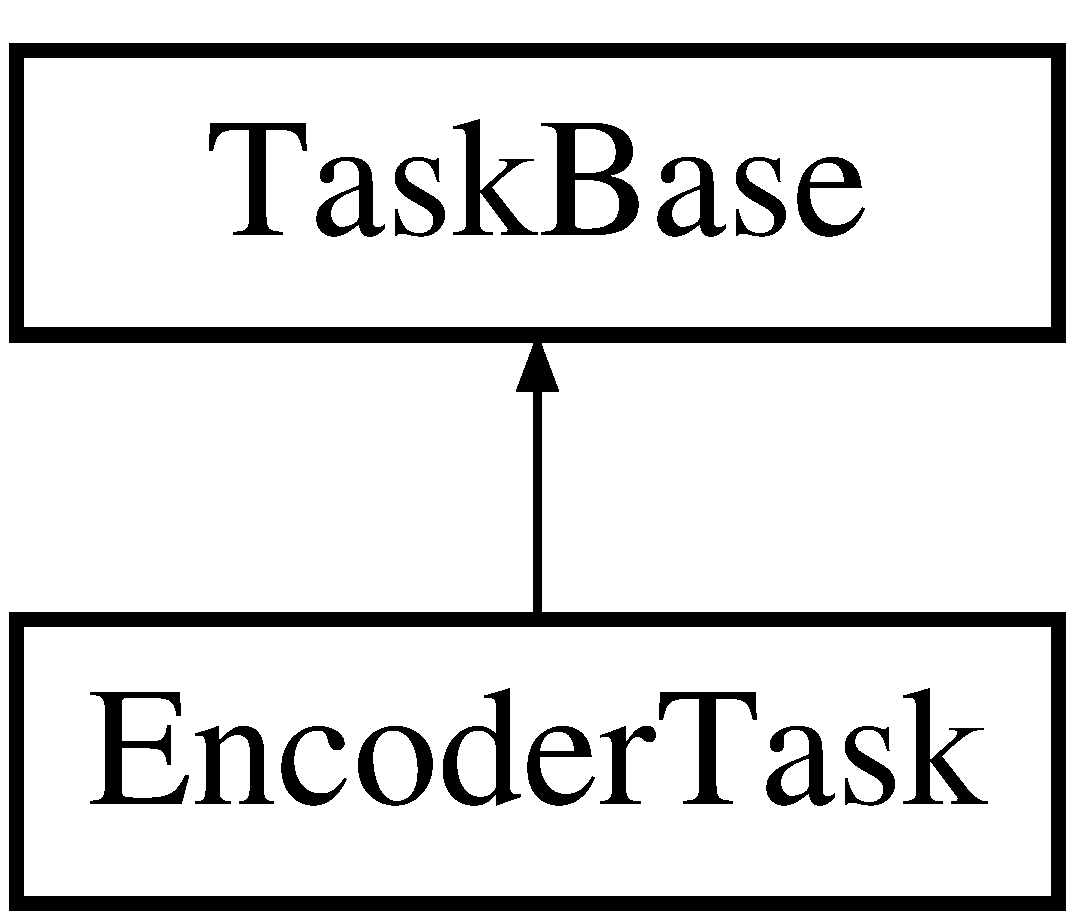
\includegraphics[height=2.000000cm]{class_encoder_task}
\end{center}
\end{figure}
\subsection*{Public Member Functions}
\begin{DoxyCompactItemize}
\item 
\mbox{\hyperlink{class_encoder_task_af40f2d1f64b159deed631cf6fd7ad26f}{Encoder\+Task}} (const char $\ast$a\+\_\+name, unsigned port\+B\+A\+S\+E\+\_\+\+T\+Y\+PE a\+\_\+priority, size\+\_\+t a\+\_\+stack\+\_\+size, \mbox{\hyperlink{classemstream}{emstream}} $\ast$p\+\_\+ser\+\_\+dev)
\begin{DoxyCompactList}\small\item\em Construct an Encoder task. \end{DoxyCompactList}\item 
void \mbox{\hyperlink{class_encoder_task_a4dfd013fe548038f941ab130adeb90fd}{run}} (void)
\begin{DoxyCompactList}\small\item\em The run method of the Encoder task that is repeatedly called by the R\+T\+OS scheduler. \end{DoxyCompactList}\end{DoxyCompactItemize}
\subsection*{Additional Inherited Members}


\subsection{Detailed Description}
Implements a task to determine the beam angle. 

This class is an extension of {\ttfamily \mbox{\hyperlink{class_task_base}{Task\+Base}}}. The purpose of the class is to determine the beam angular position and velocity. 

\subsection{Constructor \& Destructor Documentation}
\mbox{\Hypertarget{class_encoder_task_af40f2d1f64b159deed631cf6fd7ad26f}\label{class_encoder_task_af40f2d1f64b159deed631cf6fd7ad26f}} 
\index{Encoder\+Task@{Encoder\+Task}!Encoder\+Task@{Encoder\+Task}}
\index{Encoder\+Task@{Encoder\+Task}!Encoder\+Task@{Encoder\+Task}}
\subsubsection{\texorpdfstring{Encoder\+Task()}{EncoderTask()}}
{\footnotesize\ttfamily Encoder\+Task\+::\+Encoder\+Task (\begin{DoxyParamCaption}\item[{const char $\ast$}]{a\+\_\+name,  }\item[{unsigned port\+B\+A\+S\+E\+\_\+\+T\+Y\+PE}]{a\+\_\+priority,  }\item[{size\+\_\+t}]{a\+\_\+stack\+\_\+size,  }\item[{\mbox{\hyperlink{classemstream}{emstream}} $\ast$}]{p\+\_\+ser\+\_\+dev }\end{DoxyParamCaption})}



Construct an Encoder task. 

Constructor which creates and initializes an Encoder task object.

This constructor sets up the task name, priority, stack size, and serial stream. 
\begin{DoxyParams}{Parameters}
{\em a\+\_\+name} & A character string which will be the name of this task \\
\hline
{\em a\+\_\+priority} & The priority at which this task will initially run (default\+: 0) \\
\hline
{\em a\+\_\+stack\+\_\+size} & The size of this task\textquotesingle{}s stack in bytes (default\+: {\ttfamily config\+M\+I\+N\+I\+M\+A\+L\+\_\+\+S\+T\+A\+C\+K\+\_\+\+S\+I\+ZE}) \\
\hline
{\em p\+\_\+ser\+\_\+dev} & Pointer to a serial device (port, radio, SD card, etc.) which can be used by this task to communicate (default\+: N\+U\+LL)\\
\hline
\end{DoxyParams}
This constructor creates a Free\+R\+T\+OS task with the given task run function, name, priority, and stack size. Its purpose is to determine the angle of the beam based on the encoder sensor measurements. 
\begin{DoxyParams}{Parameters}
{\em a\+\_\+name} & A character string which will be the name of this task \\
\hline
{\em a\+\_\+priority} & The priority at which this task will initially run (default\+: 0) \\
\hline
{\em a\+\_\+stack\+\_\+size} & The size of this task\textquotesingle{}s stack in bytes (default\+: {\ttfamily config\+M\+I\+N\+I\+M\+A\+L\+\_\+\+S\+T\+A\+C\+K\+\_\+\+S\+I\+ZE}) \\
\hline
{\em p\+\_\+ser\+\_\+dev} & Pointer to a serial device (port, radio, SD card, etc.) which can be used by this task to communicate (default\+: N\+U\+LL) \\
\hline
\end{DoxyParams}


\subsection{Member Function Documentation}
\mbox{\Hypertarget{class_encoder_task_a4dfd013fe548038f941ab130adeb90fd}\label{class_encoder_task_a4dfd013fe548038f941ab130adeb90fd}} 
\index{Encoder\+Task@{Encoder\+Task}!run@{run}}
\index{run@{run}!Encoder\+Task@{Encoder\+Task}}
\subsubsection{\texorpdfstring{run()}{run()}}
{\footnotesize\ttfamily void Encoder\+Task\+::run (\begin{DoxyParamCaption}\item[{void}]{ }\end{DoxyParamCaption})\hspace{0.3cm}{\ttfamily [virtual]}}



The run method of the Encoder task that is repeatedly called by the R\+T\+OS scheduler. 

The {\ttfamily \mbox{\hyperlink{class_encoder_task_a4dfd013fe548038f941ab130adeb90fd}{run()}}} function for the Encoder task.

This method is called by the R\+T\+OS scheduler. The function implements a modulo positioning algorithm to account for discontinuity in the absolute position output from the encoder sensor. The encoder counts are converted to angle measurements in radians and angular velocity in rad/s. Shared variables are updated after the calculations are performed. 

Implements \mbox{\hyperlink{class_task_base_adcf6036ad9c860051ccf392ba5e7dbbc}{Task\+Base}}.



The documentation for this class was generated from the following files\+:\begin{DoxyCompactItemize}
\item 
Doxygen\+Files/\mbox{\hyperlink{_encoder_task_8h}{Encoder\+Task.\+h}}\item 
Doxygen\+Files/Encoder\+Task.\+cpp\end{DoxyCompactItemize}

\hypertarget{unionfloat__with__bits__t}{}\section{float\+\_\+with\+\_\+bits\+\_\+t Union Reference}
\label{unionfloat__with__bits__t}\index{float\+\_\+with\+\_\+bits\+\_\+t@{float\+\_\+with\+\_\+bits\+\_\+t}}


Single precision float accessed as a float or a set of 32 bits.  


\subsection*{Public Attributes}
\begin{DoxyCompactItemize}
\item 
\mbox{\Hypertarget{unionfloat__with__bits__t_a618de56b5362fe1c3e380b0d588a8910}\label{unionfloat__with__bits__t_a618de56b5362fe1c3e380b0d588a8910}} 
float \mbox{\hyperlink{unionfloat__with__bits__t_a618de56b5362fe1c3e380b0d588a8910}{number}}
\begin{DoxyCompactList}\small\item\em The floating-\/point number seen as a floating-\/point number. \end{DoxyCompactList}\item 
\mbox{\Hypertarget{unionfloat__with__bits__t_ae9649f9cee68a274f87d01f42143f92b}\label{unionfloat__with__bits__t_ae9649f9cee68a274f87d01f42143f92b}} 
int32\+\_\+t \mbox{\hyperlink{unionfloat__with__bits__t_ae9649f9cee68a274f87d01f42143f92b}{bits}}
\begin{DoxyCompactList}\small\item\em The floating-\/point number seen as a 32-\/bit integer. \end{DoxyCompactList}\end{DoxyCompactItemize}


\subsection{Detailed Description}
Single precision float accessed as a float or a set of 32 bits. 

This union is used to hold a single precision floating point number in its normal 32 bit format, but also allow the same 32 bits to be used in the format of an integer so that the sign bit, exponent, and mantissa can be accessed separately. 

The documentation for this union was generated from the following file\+:\begin{DoxyCompactItemize}
\item 
Doxygen\+Files/\mbox{\hyperlink{emstream__float_8cpp}{emstream\+\_\+float.\+cpp}}\end{DoxyCompactItemize}

\hypertarget{struct_l6206___init_type_def}{}\section{L6206\+\_\+\+Init\+Type\+Def Struct Reference}
\label{struct_l6206___init_type_def}\index{L6206\+\_\+\+Init\+Type\+Def@{L6206\+\_\+\+Init\+Type\+Def}}
\subsection*{Public Attributes}
\begin{DoxyCompactItemize}
\item 
\mbox{\Hypertarget{struct_l6206___init_type_def_a6755a71f006fc4b516210784128c2dff}\label{struct_l6206___init_type_def_a6755a71f006fc4b516210784128c2dff}} 
\mbox{\hyperlink{group___dual___full___bridge___configuration_gab5810188b32c0f4c04abcbf058f09722}{dual\+Full\+Bridge\+Config\+\_\+t}} \mbox{\hyperlink{struct_l6206___init_type_def_a6755a71f006fc4b516210784128c2dff}{config}}
\begin{DoxyCompactList}\small\item\em Bridge configuration structure. \end{DoxyCompactList}\item 
\mbox{\Hypertarget{struct_l6206___init_type_def_a7ea20fc2395b2e6d790f0e40d0c47fc1}\label{struct_l6206___init_type_def_a7ea20fc2395b2e6d790f0e40d0c47fc1}} 
uint32\+\_\+t \mbox{\hyperlink{struct_l6206___init_type_def_a7ea20fc2395b2e6d790f0e40d0c47fc1}{pwm\+Freq}}
\begin{DoxyCompactList}\small\item\em P\+WM frequency. \end{DoxyCompactList}\item 
\mbox{\Hypertarget{struct_l6206___init_type_def_a0bd6942d638b0b16ed9f1ae8871662e5}\label{struct_l6206___init_type_def_a0bd6942d638b0b16ed9f1ae8871662e5}} 
uint16\+\_\+t \mbox{\hyperlink{struct_l6206___init_type_def_a0bd6942d638b0b16ed9f1ae8871662e5}{speed}}
\begin{DoxyCompactList}\small\item\em Motor speed. \end{DoxyCompactList}\item 
\mbox{\Hypertarget{struct_l6206___init_type_def_a20047dd327627c662bb3d4301a1f2c4d}\label{struct_l6206___init_type_def_a20047dd327627c662bb3d4301a1f2c4d}} 
\mbox{\hyperlink{group___device___direction___options_ga4eaf4196e4d11d552f58f3fab218a8c7}{motor\+Dir\+\_\+t}} \mbox{\hyperlink{struct_l6206___init_type_def_a20047dd327627c662bb3d4301a1f2c4d}{direction}}
\begin{DoxyCompactList}\small\item\em Motor direction. \end{DoxyCompactList}\item 
\mbox{\Hypertarget{struct_l6206___init_type_def_a0c9583a31888ce4cae46629a94d39e8a}\label{struct_l6206___init_type_def_a0c9583a31888ce4cae46629a94d39e8a}} 
\mbox{\hyperlink{group___device___states_ga9ba865be7705688e94f95a410e917a07}{motor\+State\+\_\+t}} \mbox{\hyperlink{struct_l6206___init_type_def_a0c9583a31888ce4cae46629a94d39e8a}{motion\+State}}
\begin{DoxyCompactList}\small\item\em Current motor state. \end{DoxyCompactList}\item 
\mbox{\Hypertarget{struct_l6206___init_type_def_a324c04f52dce5aafe3fc3542228e8978}\label{struct_l6206___init_type_def_a324c04f52dce5aafe3fc3542228e8978}} 
\mbox{\hyperlink{group___motor___boolean___type_ga0ecf26b576b9a54eca656b9be7ba6a06}{bool}} \mbox{\hyperlink{struct_l6206___init_type_def_a324c04f52dce5aafe3fc3542228e8978}{bridge\+Enabled}}
\begin{DoxyCompactList}\small\item\em Bridge enabled (true) or not (false) \end{DoxyCompactList}\end{DoxyCompactItemize}


The documentation for this struct was generated from the following file\+:\begin{DoxyCompactItemize}
\item 
Doxygen\+Files/\mbox{\hyperlink{l6206_8h}{l6206.\+h}}\end{DoxyCompactItemize}

\hypertarget{class_limit_switch_task}{}\section{Limit\+Switch\+Task Class Reference}
\label{class_limit_switch_task}\index{Limit\+Switch\+Task@{Limit\+Switch\+Task}}


Implements a task to determine whether or not the system is safe.  




{\ttfamily \#include $<$Limit\+Switch\+Task.\+h$>$}

Inheritance diagram for Limit\+Switch\+Task\+:\begin{figure}[H]
\begin{center}
\leavevmode
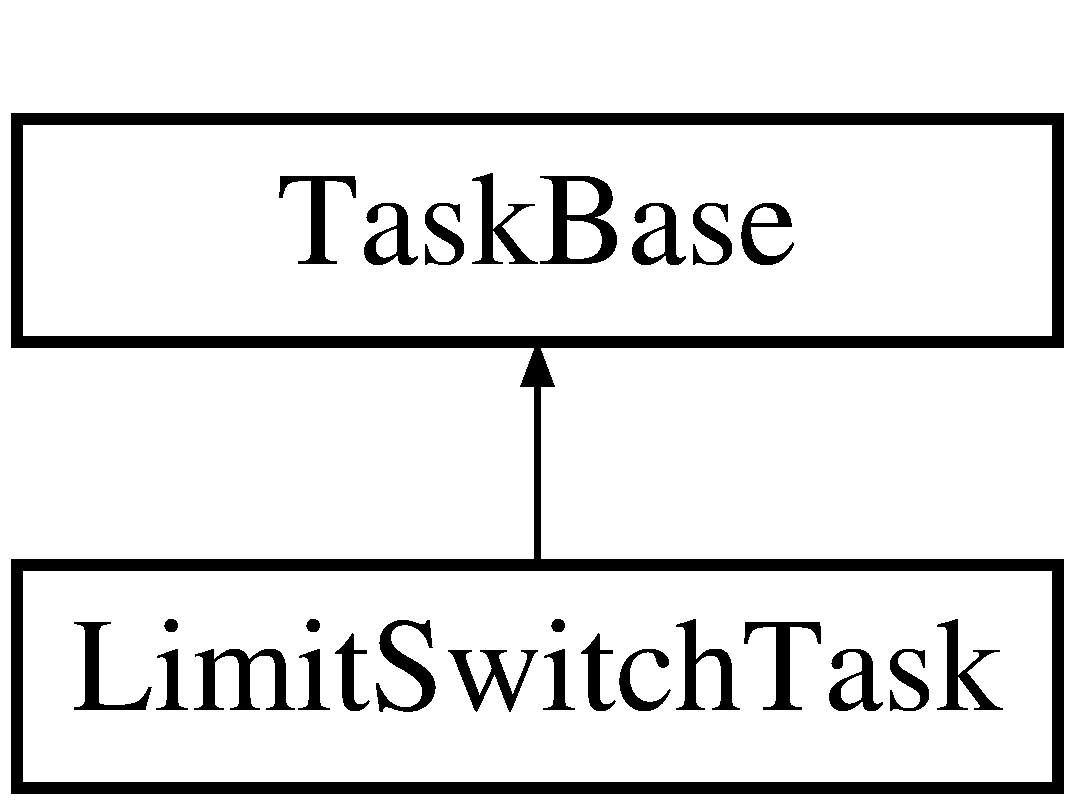
\includegraphics[height=2.000000cm]{class_limit_switch_task}
\end{center}
\end{figure}
\subsection*{Public Member Functions}
\begin{DoxyCompactItemize}
\item 
\mbox{\hyperlink{class_limit_switch_task_a77a868a88b718c91292284e569f24b59}{Limit\+Switch\+Task}} (const char $\ast$a\+\_\+name, unsigned port\+B\+A\+S\+E\+\_\+\+T\+Y\+PE a\+\_\+priority, size\+\_\+t a\+\_\+stack\+\_\+size, \mbox{\hyperlink{classemstream}{emstream}} $\ast$p\+\_\+ser\+\_\+dev)
\begin{DoxyCompactList}\small\item\em Construct a Limit\+Switch task. \end{DoxyCompactList}\item 
void \mbox{\hyperlink{class_limit_switch_task_abf943a0f6ab5ab5fa9588f9cdbc6bc82}{run}} (void)
\begin{DoxyCompactList}\small\item\em The run method of the Limit\+Switch task that is repeatedly called by the R\+T\+OS scheduler. \end{DoxyCompactList}\end{DoxyCompactItemize}
\subsection*{Additional Inherited Members}


\subsection{Detailed Description}
Implements a task to determine whether or not the system is safe. 

This class is an extension of {\ttfamily \mbox{\hyperlink{class_task_base}{Task\+Base}}}. The purpose of the class is to stop the motor if a limit switch is triggered, meaning the system is currently in an unsafe condition. 

\subsection{Constructor \& Destructor Documentation}
\mbox{\Hypertarget{class_limit_switch_task_a77a868a88b718c91292284e569f24b59}\label{class_limit_switch_task_a77a868a88b718c91292284e569f24b59}} 
\index{Limit\+Switch\+Task@{Limit\+Switch\+Task}!Limit\+Switch\+Task@{Limit\+Switch\+Task}}
\index{Limit\+Switch\+Task@{Limit\+Switch\+Task}!Limit\+Switch\+Task@{Limit\+Switch\+Task}}
\subsubsection{\texorpdfstring{Limit\+Switch\+Task()}{LimitSwitchTask()}}
{\footnotesize\ttfamily Limit\+Switch\+Task\+::\+Limit\+Switch\+Task (\begin{DoxyParamCaption}\item[{const char $\ast$}]{a\+\_\+name,  }\item[{unsigned port\+B\+A\+S\+E\+\_\+\+T\+Y\+PE}]{a\+\_\+priority,  }\item[{size\+\_\+t}]{a\+\_\+stack\+\_\+size,  }\item[{\mbox{\hyperlink{classemstream}{emstream}} $\ast$}]{p\+\_\+ser\+\_\+dev }\end{DoxyParamCaption})}



Construct a Limit\+Switch task. 

Constructor which creates and initializes a Limit\+Switch task object.

This constructor sets up the task name, priority, stack size, and serial stream. 
\begin{DoxyParams}{Parameters}
{\em a\+\_\+name} & A character string which will be the name of this task \\
\hline
{\em a\+\_\+priority} & The priority at which this task will initially run (default\+: 0) \\
\hline
{\em a\+\_\+stack\+\_\+size} & The size of this task\textquotesingle{}s stack in bytes (default\+: {\ttfamily config\+M\+I\+N\+I\+M\+A\+L\+\_\+\+S\+T\+A\+C\+K\+\_\+\+S\+I\+ZE}) \\
\hline
{\em p\+\_\+ser\+\_\+dev} & Pointer to a serial device (port, radio, SD card, etc.) which can be used by this task to communicate (default\+: N\+U\+LL)\\
\hline
\end{DoxyParams}
This constructor creates a Free\+R\+T\+OS task with the given task run function, name, priority, and stack size. Its purpose is to alarm the system of an unsafe condition if a limit switch drives a digital pin low. 
\begin{DoxyParams}{Parameters}
{\em a\+\_\+name} & A character string which will be the name of this task \\
\hline
{\em a\+\_\+priority} & The priority at which this task will initially run (default\+: 0) \\
\hline
{\em a\+\_\+stack\+\_\+size} & The size of this task\textquotesingle{}s stack in bytes (default\+: {\ttfamily config\+M\+I\+N\+I\+M\+A\+L\+\_\+\+S\+T\+A\+C\+K\+\_\+\+S\+I\+ZE}) \\
\hline
{\em p\+\_\+ser\+\_\+dev} & Pointer to a serial device (port, radio, SD card, etc.) which can be used by this task to communicate (default\+: N\+U\+LL) \\
\hline
\end{DoxyParams}


\subsection{Member Function Documentation}
\mbox{\Hypertarget{class_limit_switch_task_abf943a0f6ab5ab5fa9588f9cdbc6bc82}\label{class_limit_switch_task_abf943a0f6ab5ab5fa9588f9cdbc6bc82}} 
\index{Limit\+Switch\+Task@{Limit\+Switch\+Task}!run@{run}}
\index{run@{run}!Limit\+Switch\+Task@{Limit\+Switch\+Task}}
\subsubsection{\texorpdfstring{run()}{run()}}
{\footnotesize\ttfamily void Limit\+Switch\+Task\+::run (\begin{DoxyParamCaption}\item[{void}]{ }\end{DoxyParamCaption})\hspace{0.3cm}{\ttfamily [virtual]}}



The run method of the Limit\+Switch task that is repeatedly called by the R\+T\+OS scheduler. 

The {\ttfamily \mbox{\hyperlink{class_limit_switch_task_abf943a0f6ab5ab5fa9588f9cdbc6bc82}{run()}}} function for the Limit\+Switch task.

This method is called by the R\+T\+OS scheduler. The function reads a G\+P\+IO pin and triggers an unsafe condition if the pin is pulled low. The condition is updated in the p\+\_\+safe shared variable. 

Implements \mbox{\hyperlink{class_task_base_adcf6036ad9c860051ccf392ba5e7dbbc}{Task\+Base}}.



The documentation for this class was generated from the following files\+:\begin{DoxyCompactItemize}
\item 
Doxygen\+Files/\mbox{\hyperlink{_limit_switch_task_8h}{Limit\+Switch\+Task.\+h}}\item 
Doxygen\+Files/Limit\+Switch\+Task.\+cpp\end{DoxyCompactItemize}

\hypertarget{class_motor_drive_task}{}\section{Motor\+Drive\+Task Class Reference}
\label{class_motor_drive_task}\index{Motor\+Drive\+Task@{Motor\+Drive\+Task}}


Implements a task to control the motor.  




{\ttfamily \#include $<$Motor\+Drive\+Task.\+h$>$}

Inheritance diagram for Motor\+Drive\+Task\+:\begin{figure}[H]
\begin{center}
\leavevmode
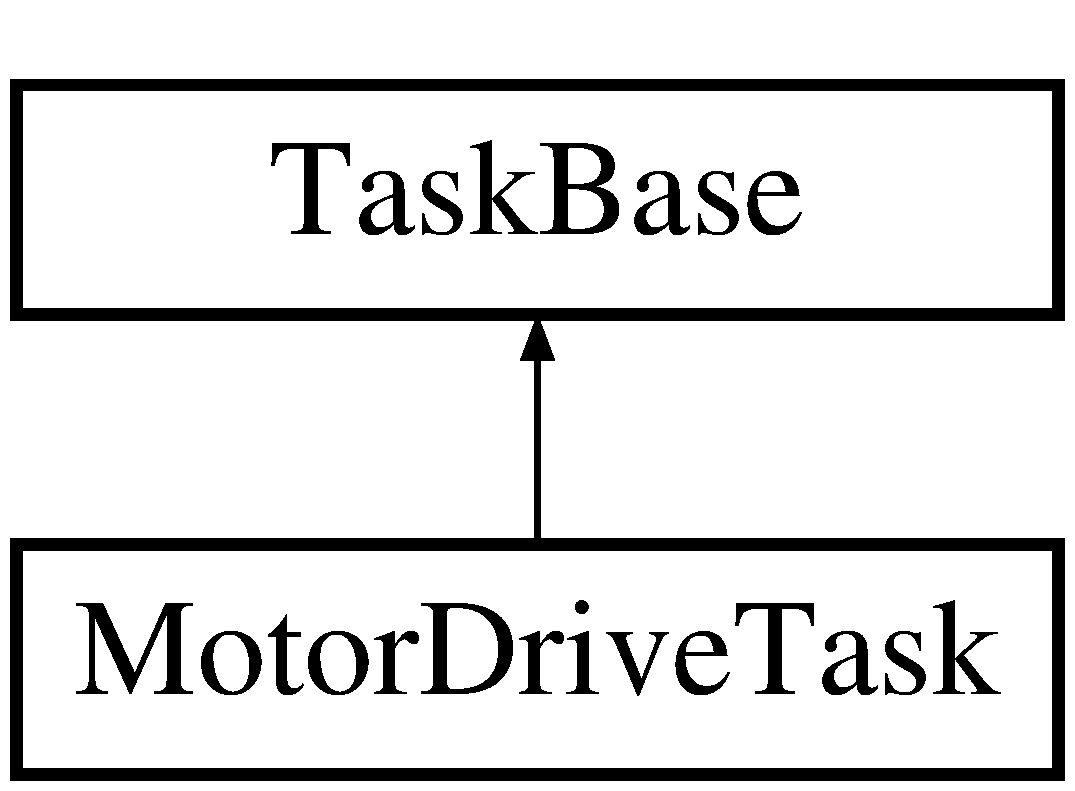
\includegraphics[height=2.000000cm]{class_motor_drive_task}
\end{center}
\end{figure}
\subsection*{Public Member Functions}
\begin{DoxyCompactItemize}
\item 
\mbox{\hyperlink{class_motor_drive_task_ae97b28489a97e5f365a5d27156153f0e}{Motor\+Drive\+Task}} (const char $\ast$a\+\_\+name, unsigned port\+B\+A\+S\+E\+\_\+\+T\+Y\+PE a\+\_\+priority, size\+\_\+t a\+\_\+stack\+\_\+size, \mbox{\hyperlink{classemstream}{emstream}} $\ast$p\+\_\+ser\+\_\+dev)
\begin{DoxyCompactList}\small\item\em Construct a Motor\+Drive task. \end{DoxyCompactList}\item 
void \mbox{\hyperlink{class_motor_drive_task_abc617fef420f9dc8cdd6144d8d7adea8}{run}} (void)
\begin{DoxyCompactList}\small\item\em The run method of the Motor\+Drive task that is repeatedly called by the R\+T\+OS scheduler. \end{DoxyCompactList}\end{DoxyCompactItemize}
\subsection*{Additional Inherited Members}


\subsection{Detailed Description}
Implements a task to control the motor. 

This class is an extension of {\ttfamily \mbox{\hyperlink{class_task_base}{Task\+Base}}}. The purpose of the class is to interface with the motor driver to control the direction and operating condition of the brushed DC motor. 

\subsection{Constructor \& Destructor Documentation}
\mbox{\Hypertarget{class_motor_drive_task_ae97b28489a97e5f365a5d27156153f0e}\label{class_motor_drive_task_ae97b28489a97e5f365a5d27156153f0e}} 
\index{Motor\+Drive\+Task@{Motor\+Drive\+Task}!Motor\+Drive\+Task@{Motor\+Drive\+Task}}
\index{Motor\+Drive\+Task@{Motor\+Drive\+Task}!Motor\+Drive\+Task@{Motor\+Drive\+Task}}
\subsubsection{\texorpdfstring{Motor\+Drive\+Task()}{MotorDriveTask()}}
{\footnotesize\ttfamily Motor\+Drive\+Task\+::\+Motor\+Drive\+Task (\begin{DoxyParamCaption}\item[{const char $\ast$}]{a\+\_\+name,  }\item[{unsigned port\+B\+A\+S\+E\+\_\+\+T\+Y\+PE}]{a\+\_\+priority,  }\item[{size\+\_\+t}]{a\+\_\+stack\+\_\+size,  }\item[{\mbox{\hyperlink{classemstream}{emstream}} $\ast$}]{p\+\_\+ser\+\_\+dev }\end{DoxyParamCaption})}



Construct a Motor\+Drive task. 

Constructor which creates and initializes a Motor\+Drive task object.

This constructor sets up the task name, priority, stack size, and serial stream. 
\begin{DoxyParams}{Parameters}
{\em a\+\_\+name} & A character string which will be the name of this task \\
\hline
{\em a\+\_\+priority} & The priority at which this task will initially run (default\+: 0) \\
\hline
{\em a\+\_\+stack\+\_\+size} & The size of this task\textquotesingle{}s stack in bytes (default\+: {\ttfamily config\+M\+I\+N\+I\+M\+A\+L\+\_\+\+S\+T\+A\+C\+K\+\_\+\+S\+I\+ZE}) \\
\hline
{\em p\+\_\+ser\+\_\+dev} & Pointer to a serial device (port, radio, SD card, etc.) which can be used by this task to communicate (default\+: N\+U\+LL)\\
\hline
\end{DoxyParams}
This constructor creates a Free\+R\+T\+OS task with the given task run function, name, priority, and stack size. Its purpose is to set the appropriate motor driver pins depending on the P\+WM command, and shut down the motor if an unsafe condition was detected. 
\begin{DoxyParams}{Parameters}
{\em a\+\_\+name} & A character string which will be the name of this task \\
\hline
{\em a\+\_\+priority} & The priority at which this task will initially run (default\+: 0) \\
\hline
{\em a\+\_\+stack\+\_\+size} & The size of this task\textquotesingle{}s stack in bytes (default\+: {\ttfamily config\+M\+I\+N\+I\+M\+A\+L\+\_\+\+S\+T\+A\+C\+K\+\_\+\+S\+I\+ZE}) \\
\hline
{\em p\+\_\+ser\+\_\+dev} & Pointer to a serial device (port, radio, SD card, etc.) which can be used by this task to communicate (default\+: N\+U\+LL) \\
\hline
\end{DoxyParams}


\subsection{Member Function Documentation}
\mbox{\Hypertarget{class_motor_drive_task_abc617fef420f9dc8cdd6144d8d7adea8}\label{class_motor_drive_task_abc617fef420f9dc8cdd6144d8d7adea8}} 
\index{Motor\+Drive\+Task@{Motor\+Drive\+Task}!run@{run}}
\index{run@{run}!Motor\+Drive\+Task@{Motor\+Drive\+Task}}
\subsubsection{\texorpdfstring{run()}{run()}}
{\footnotesize\ttfamily void Motor\+Drive\+Task\+::run (\begin{DoxyParamCaption}\item[{void}]{ }\end{DoxyParamCaption})\hspace{0.3cm}{\ttfamily [virtual]}}



The run method of the Motor\+Drive task that is repeatedly called by the R\+T\+OS scheduler. 

The {\ttfamily \mbox{\hyperlink{class_motor_drive_task_abc617fef420f9dc8cdd6144d8d7adea8}{run()}}} function for the Motor\+Drive task.

This method is called by the R\+T\+OS scheduler. The function sets the IN pins on the motor driver to define the direction of the motor, depending on the sign of the P\+WM signal. If there\textquotesingle{}s an unsafe condition, the motor driver will be set to B\+R\+A\+KE mode by pulling the IN pins low. 

Implements \mbox{\hyperlink{class_task_base_adcf6036ad9c860051ccf392ba5e7dbbc}{Task\+Base}}.



The documentation for this class was generated from the following files\+:\begin{DoxyCompactItemize}
\item 
Doxygen\+Files/\mbox{\hyperlink{_motor_drive_task_8h}{Motor\+Drive\+Task.\+h}}\item 
Doxygen\+Files/Motor\+Drive\+Task.\+cpp\end{DoxyCompactItemize}

\hypertarget{structmotor_drv__t}{}\section{motor\+Drv\+\_\+t Struct Reference}
\label{structmotor_drv__t}\index{motor\+Drv\+\_\+t@{motor\+Drv\+\_\+t}}


Motor driver structure definition.  




{\ttfamily \#include $<$motor.\+h$>$}

\subsection*{Public Attributes}
\begin{DoxyCompactItemize}
\item 
\mbox{\Hypertarget{structmotor_drv__t_a86d3d3dbef0e0f1698e1efe954532141}\label{structmotor_drv__t_a86d3d3dbef0e0f1698e1efe954532141}} 
void($\ast$ \mbox{\hyperlink{structmotor_drv__t_a86d3d3dbef0e0f1698e1efe954532141}{Init}} )(void $\ast$)
\begin{DoxyCompactList}\small\item\em Function pointer to Init. \end{DoxyCompactList}\item 
\mbox{\Hypertarget{structmotor_drv__t_af319b5a6dc66a750bd942d543586e4dc}\label{structmotor_drv__t_af319b5a6dc66a750bd942d543586e4dc}} 
uint16\+\_\+t($\ast$ \mbox{\hyperlink{structmotor_drv__t_af319b5a6dc66a750bd942d543586e4dc}{Read\+ID}} )(void)
\begin{DoxyCompactList}\small\item\em Function pointer to Read\+ID. \end{DoxyCompactList}\item 
\mbox{\Hypertarget{structmotor_drv__t_a2b3cb9cf36826feabf6fe3c0b4bbc48b}\label{structmotor_drv__t_a2b3cb9cf36826feabf6fe3c0b4bbc48b}} 
void($\ast$ \mbox{\hyperlink{structmotor_drv__t_a2b3cb9cf36826feabf6fe3c0b4bbc48b}{Attach\+Error\+Handler}} )(void($\ast$callback)(uint16\+\_\+t))
\begin{DoxyCompactList}\small\item\em Function pointer to Attach\+Error\+Handler. \end{DoxyCompactList}\item 
\mbox{\Hypertarget{structmotor_drv__t_ae648f05bb2bc6e5f85da182eedaeca82}\label{structmotor_drv__t_ae648f05bb2bc6e5f85da182eedaeca82}} 
void($\ast$ \mbox{\hyperlink{structmotor_drv__t_ae648f05bb2bc6e5f85da182eedaeca82}{Attach\+Flag\+Interrupt}} )(void($\ast$callback)(void))
\begin{DoxyCompactList}\small\item\em Function pointer to Attach\+Flag\+Interrupt. \end{DoxyCompactList}\item 
\mbox{\Hypertarget{structmotor_drv__t_a093d8ad30fd271e344195dbde36b8a2e}\label{structmotor_drv__t_a093d8ad30fd271e344195dbde36b8a2e}} 
void($\ast$ \mbox{\hyperlink{structmotor_drv__t_a093d8ad30fd271e344195dbde36b8a2e}{Attach\+Busy\+Interrupt}} )(void($\ast$callback)(void))
\begin{DoxyCompactList}\small\item\em Function pointer to Attach\+Busy\+Interrupt. \end{DoxyCompactList}\item 
\mbox{\Hypertarget{structmotor_drv__t_ab2dfca0996212691221964294195a441}\label{structmotor_drv__t_ab2dfca0996212691221964294195a441}} 
void($\ast$ \mbox{\hyperlink{structmotor_drv__t_ab2dfca0996212691221964294195a441}{Flag\+Interrupt\+Handler}} )(void)
\begin{DoxyCompactList}\small\item\em Function pointer to Flag\+Interrupt\+Handler. \end{DoxyCompactList}\item 
\mbox{\Hypertarget{structmotor_drv__t_a371a0207f336ecb38bd0fdb047b8c683}\label{structmotor_drv__t_a371a0207f336ecb38bd0fdb047b8c683}} 
uint16\+\_\+t($\ast$ \mbox{\hyperlink{structmotor_drv__t_a371a0207f336ecb38bd0fdb047b8c683}{Get\+Acceleration}} )(uint8\+\_\+t)
\begin{DoxyCompactList}\small\item\em Function pointer to Get\+Acceleration. \end{DoxyCompactList}\item 
\mbox{\Hypertarget{structmotor_drv__t_a2c2ce036e0f91aac0658806665c68361}\label{structmotor_drv__t_a2c2ce036e0f91aac0658806665c68361}} 
uint16\+\_\+t($\ast$ \mbox{\hyperlink{structmotor_drv__t_a2c2ce036e0f91aac0658806665c68361}{Get\+Current\+Speed}} )(uint8\+\_\+t)
\begin{DoxyCompactList}\small\item\em Function pointer to Get\+Current\+Speed. \end{DoxyCompactList}\item 
\mbox{\Hypertarget{structmotor_drv__t_a82d706c0ca281f85f83f65e5b3ecb747}\label{structmotor_drv__t_a82d706c0ca281f85f83f65e5b3ecb747}} 
uint16\+\_\+t($\ast$ \mbox{\hyperlink{structmotor_drv__t_a82d706c0ca281f85f83f65e5b3ecb747}{Get\+Deceleration}} )(uint8\+\_\+t)
\begin{DoxyCompactList}\small\item\em Function pointer to Get\+Deceleration. \end{DoxyCompactList}\item 
\mbox{\Hypertarget{structmotor_drv__t_aa035813a35bb5a589891b6879c88f5cf}\label{structmotor_drv__t_aa035813a35bb5a589891b6879c88f5cf}} 
\mbox{\hyperlink{group___device___states_ga9ba865be7705688e94f95a410e917a07}{motor\+State\+\_\+t}}($\ast$ \mbox{\hyperlink{structmotor_drv__t_aa035813a35bb5a589891b6879c88f5cf}{Get\+Device\+State}} )(uint8\+\_\+t)
\begin{DoxyCompactList}\small\item\em Function pointer to Get\+Device\+State. \end{DoxyCompactList}\item 
\mbox{\Hypertarget{structmotor_drv__t_aaa6c85b99a40f6ebb4bc22647afd814e}\label{structmotor_drv__t_aaa6c85b99a40f6ebb4bc22647afd814e}} 
uint32\+\_\+t($\ast$ \mbox{\hyperlink{structmotor_drv__t_aaa6c85b99a40f6ebb4bc22647afd814e}{Get\+Fw\+Version}} )(void)
\begin{DoxyCompactList}\small\item\em Function pointer to Get\+Fw\+Version. \end{DoxyCompactList}\item 
\mbox{\Hypertarget{structmotor_drv__t_ab8d2a9b8286ea9781035e30e887264a6}\label{structmotor_drv__t_ab8d2a9b8286ea9781035e30e887264a6}} 
int32\+\_\+t($\ast$ \mbox{\hyperlink{structmotor_drv__t_ab8d2a9b8286ea9781035e30e887264a6}{Get\+Mark}} )(uint8\+\_\+t)
\begin{DoxyCompactList}\small\item\em Function pointer to Get\+Mark. \end{DoxyCompactList}\item 
\mbox{\Hypertarget{structmotor_drv__t_aa34c04b174fdaf1e53e6796ffb7b9c7b}\label{structmotor_drv__t_aa34c04b174fdaf1e53e6796ffb7b9c7b}} 
uint16\+\_\+t($\ast$ \mbox{\hyperlink{structmotor_drv__t_aa34c04b174fdaf1e53e6796ffb7b9c7b}{Get\+Max\+Speed}} )(uint8\+\_\+t)
\begin{DoxyCompactList}\small\item\em Function pointer to Get\+Max\+Speed. \end{DoxyCompactList}\item 
\mbox{\Hypertarget{structmotor_drv__t_a93c3923b625321220442f8175daf39aa}\label{structmotor_drv__t_a93c3923b625321220442f8175daf39aa}} 
uint16\+\_\+t($\ast$ \mbox{\hyperlink{structmotor_drv__t_a93c3923b625321220442f8175daf39aa}{Get\+Min\+Speed}} )(uint8\+\_\+t)
\begin{DoxyCompactList}\small\item\em Function pointer to Get\+Min\+Speed. \end{DoxyCompactList}\item 
\mbox{\Hypertarget{structmotor_drv__t_a54c0c8b2813c4e0bca29a988ee909837}\label{structmotor_drv__t_a54c0c8b2813c4e0bca29a988ee909837}} 
int32\+\_\+t($\ast$ \mbox{\hyperlink{structmotor_drv__t_a54c0c8b2813c4e0bca29a988ee909837}{Get\+Position}} )(uint8\+\_\+t)
\begin{DoxyCompactList}\small\item\em Function pointer to Get\+Position. \end{DoxyCompactList}\item 
\mbox{\Hypertarget{structmotor_drv__t_af5c8f1332b37d2b5280e013b1c5cc8e1}\label{structmotor_drv__t_af5c8f1332b37d2b5280e013b1c5cc8e1}} 
void($\ast$ \mbox{\hyperlink{structmotor_drv__t_af5c8f1332b37d2b5280e013b1c5cc8e1}{Go\+Home}} )(uint8\+\_\+t)
\begin{DoxyCompactList}\small\item\em Function pointer to Go\+Home. \end{DoxyCompactList}\item 
\mbox{\Hypertarget{structmotor_drv__t_a2e2cf9c800cbda999492268990d8183b}\label{structmotor_drv__t_a2e2cf9c800cbda999492268990d8183b}} 
void($\ast$ \mbox{\hyperlink{structmotor_drv__t_a2e2cf9c800cbda999492268990d8183b}{Go\+Mark}} )(uint8\+\_\+t)
\begin{DoxyCompactList}\small\item\em Function pointer to Go\+Mark. \end{DoxyCompactList}\item 
\mbox{\Hypertarget{structmotor_drv__t_ab6cfea0a721c044897747a516f90083c}\label{structmotor_drv__t_ab6cfea0a721c044897747a516f90083c}} 
void($\ast$ \mbox{\hyperlink{structmotor_drv__t_ab6cfea0a721c044897747a516f90083c}{Go\+To}} )(uint8\+\_\+t, int32\+\_\+t)
\begin{DoxyCompactList}\small\item\em Function pointer to Go\+To. \end{DoxyCompactList}\item 
\mbox{\Hypertarget{structmotor_drv__t_ab4a3ff09a8427ee9b4105b1d15e77dde}\label{structmotor_drv__t_ab4a3ff09a8427ee9b4105b1d15e77dde}} 
void($\ast$ \mbox{\hyperlink{structmotor_drv__t_ab4a3ff09a8427ee9b4105b1d15e77dde}{Hard\+Stop}} )(uint8\+\_\+t)
\begin{DoxyCompactList}\small\item\em Function pointer to Hard\+Stop. \end{DoxyCompactList}\item 
\mbox{\Hypertarget{structmotor_drv__t_a9b1991e0a87bc5c628cda5a5eee5e061}\label{structmotor_drv__t_a9b1991e0a87bc5c628cda5a5eee5e061}} 
void($\ast$ \mbox{\hyperlink{structmotor_drv__t_a9b1991e0a87bc5c628cda5a5eee5e061}{Move}} )(uint8\+\_\+t, \mbox{\hyperlink{group___device___direction___options_ga4eaf4196e4d11d552f58f3fab218a8c7}{motor\+Dir\+\_\+t}}, uint32\+\_\+t)
\begin{DoxyCompactList}\small\item\em Function pointer to Move. \end{DoxyCompactList}\item 
\mbox{\Hypertarget{structmotor_drv__t_ada59618cf876177c4a9afd5c82dcf52b}\label{structmotor_drv__t_ada59618cf876177c4a9afd5c82dcf52b}} 
void($\ast$ \mbox{\hyperlink{structmotor_drv__t_ada59618cf876177c4a9afd5c82dcf52b}{Reset\+All\+Devices}} )(void)
\begin{DoxyCompactList}\small\item\em Function pointer to Reset\+All\+Devices. \end{DoxyCompactList}\item 
\mbox{\Hypertarget{structmotor_drv__t_a5d3aa777ac329db7380bd002897e03fe}\label{structmotor_drv__t_a5d3aa777ac329db7380bd002897e03fe}} 
void($\ast$ \mbox{\hyperlink{structmotor_drv__t_a5d3aa777ac329db7380bd002897e03fe}{Run}} )(uint8\+\_\+t, \mbox{\hyperlink{group___device___direction___options_ga4eaf4196e4d11d552f58f3fab218a8c7}{motor\+Dir\+\_\+t}})
\begin{DoxyCompactList}\small\item\em Function pointer to Run. \end{DoxyCompactList}\item 
\mbox{\Hypertarget{structmotor_drv__t_a0c1b8bf57ee1d81256947a527d89dd63}\label{structmotor_drv__t_a0c1b8bf57ee1d81256947a527d89dd63}} 
\mbox{\hyperlink{group___motor___boolean___type_ga0ecf26b576b9a54eca656b9be7ba6a06}{bool}}($\ast$ \mbox{\hyperlink{structmotor_drv__t_a0c1b8bf57ee1d81256947a527d89dd63}{Set\+Acceleration}} )(uint8\+\_\+t, uint16\+\_\+t)
\begin{DoxyCompactList}\small\item\em Function pointer to Set\+Acceleration. \end{DoxyCompactList}\item 
\mbox{\Hypertarget{structmotor_drv__t_a566ac7824184db95a98f7e7616c99510}\label{structmotor_drv__t_a566ac7824184db95a98f7e7616c99510}} 
\mbox{\hyperlink{group___motor___boolean___type_ga0ecf26b576b9a54eca656b9be7ba6a06}{bool}}($\ast$ \mbox{\hyperlink{structmotor_drv__t_a566ac7824184db95a98f7e7616c99510}{Set\+Deceleration}} )(uint8\+\_\+t, uint16\+\_\+t)
\begin{DoxyCompactList}\small\item\em Function pointer to Set\+Deceleration. \end{DoxyCompactList}\item 
\mbox{\Hypertarget{structmotor_drv__t_a7abd7a1f16f8a2d7cf765839117c30ac}\label{structmotor_drv__t_a7abd7a1f16f8a2d7cf765839117c30ac}} 
void($\ast$ \mbox{\hyperlink{structmotor_drv__t_a7abd7a1f16f8a2d7cf765839117c30ac}{Set\+Home}} )(uint8\+\_\+t, int32\+\_\+t)
\begin{DoxyCompactList}\small\item\em Function pointer to Set\+Home. \end{DoxyCompactList}\item 
\mbox{\Hypertarget{structmotor_drv__t_a06ca8c0b37f2a095e3aa5d233d5a91ed}\label{structmotor_drv__t_a06ca8c0b37f2a095e3aa5d233d5a91ed}} 
void($\ast$ \mbox{\hyperlink{structmotor_drv__t_a06ca8c0b37f2a095e3aa5d233d5a91ed}{Set\+Mark}} )(uint8\+\_\+t, int32\+\_\+t)
\begin{DoxyCompactList}\small\item\em Function pointer to Set\+Mark. \end{DoxyCompactList}\item 
\mbox{\Hypertarget{structmotor_drv__t_a9894eb824a9b74e994a547f15fbb03fa}\label{structmotor_drv__t_a9894eb824a9b74e994a547f15fbb03fa}} 
\mbox{\hyperlink{group___motor___boolean___type_ga0ecf26b576b9a54eca656b9be7ba6a06}{bool}}($\ast$ \mbox{\hyperlink{structmotor_drv__t_a9894eb824a9b74e994a547f15fbb03fa}{Set\+Max\+Speed}} )(uint8\+\_\+t, uint16\+\_\+t)
\begin{DoxyCompactList}\small\item\em Function pointer to Set\+Max\+Speed. \end{DoxyCompactList}\item 
\mbox{\Hypertarget{structmotor_drv__t_a925736ee04f781c5692db377a7b61fff}\label{structmotor_drv__t_a925736ee04f781c5692db377a7b61fff}} 
\mbox{\hyperlink{group___motor___boolean___type_ga0ecf26b576b9a54eca656b9be7ba6a06}{bool}}($\ast$ \mbox{\hyperlink{structmotor_drv__t_a925736ee04f781c5692db377a7b61fff}{Set\+Min\+Speed}} )(uint8\+\_\+t, uint16\+\_\+t)
\begin{DoxyCompactList}\small\item\em Function pointer to Set\+Min\+Speed. \end{DoxyCompactList}\item 
\mbox{\Hypertarget{structmotor_drv__t_a49de3f6a7489c5df4f8c3c1c11b98bf4}\label{structmotor_drv__t_a49de3f6a7489c5df4f8c3c1c11b98bf4}} 
\mbox{\hyperlink{group___motor___boolean___type_ga0ecf26b576b9a54eca656b9be7ba6a06}{bool}}($\ast$ \mbox{\hyperlink{structmotor_drv__t_a49de3f6a7489c5df4f8c3c1c11b98bf4}{Soft\+Stop}} )(uint8\+\_\+t)
\begin{DoxyCompactList}\small\item\em Function pointer to Soft\+Stop. \end{DoxyCompactList}\item 
\mbox{\Hypertarget{structmotor_drv__t_a9fedff6ee533edfc8a75ca5e4fbe2ea5}\label{structmotor_drv__t_a9fedff6ee533edfc8a75ca5e4fbe2ea5}} 
void($\ast$ \mbox{\hyperlink{structmotor_drv__t_a9fedff6ee533edfc8a75ca5e4fbe2ea5}{Step\+Clock\+Handler}} )(uint8\+\_\+t device\+Id)
\begin{DoxyCompactList}\small\item\em Function pointer to Step\+Clock\+Handler. \end{DoxyCompactList}\item 
\mbox{\Hypertarget{structmotor_drv__t_a4648533c2f0a7d304f8aa4fc1810024b}\label{structmotor_drv__t_a4648533c2f0a7d304f8aa4fc1810024b}} 
void($\ast$ \mbox{\hyperlink{structmotor_drv__t_a4648533c2f0a7d304f8aa4fc1810024b}{Wait\+While\+Active}} )(uint8\+\_\+t)
\begin{DoxyCompactList}\small\item\em Function pointer to Wait\+While\+Active. \end{DoxyCompactList}\item 
\mbox{\Hypertarget{structmotor_drv__t_a740c93c53fa9671d2e76c430ccfa5d2f}\label{structmotor_drv__t_a740c93c53fa9671d2e76c430ccfa5d2f}} 
void($\ast$ \mbox{\hyperlink{structmotor_drv__t_a740c93c53fa9671d2e76c430ccfa5d2f}{Cmd\+Disable}} )(uint8\+\_\+t)
\begin{DoxyCompactList}\small\item\em Function pointer to Cmd\+Disable. \end{DoxyCompactList}\item 
\mbox{\Hypertarget{structmotor_drv__t_a605ce46f3786e1eea7b173905440832b}\label{structmotor_drv__t_a605ce46f3786e1eea7b173905440832b}} 
void($\ast$ \mbox{\hyperlink{structmotor_drv__t_a605ce46f3786e1eea7b173905440832b}{Cmd\+Enable}} )(uint8\+\_\+t)
\begin{DoxyCompactList}\small\item\em Function pointer to Cmd\+Enable. \end{DoxyCompactList}\item 
\mbox{\Hypertarget{structmotor_drv__t_a8d55886dbf2c2c18fdd01f3028a93c07}\label{structmotor_drv__t_a8d55886dbf2c2c18fdd01f3028a93c07}} 
uint32\+\_\+t($\ast$ \mbox{\hyperlink{structmotor_drv__t_a8d55886dbf2c2c18fdd01f3028a93c07}{Cmd\+Get\+Param}} )(uint8\+\_\+t, uint32\+\_\+t)
\begin{DoxyCompactList}\small\item\em Function pointer to Cmd\+Get\+Param. \end{DoxyCompactList}\item 
\mbox{\Hypertarget{structmotor_drv__t_a239f7eaa897de7ec050be6cb4a4e57e4}\label{structmotor_drv__t_a239f7eaa897de7ec050be6cb4a4e57e4}} 
uint16\+\_\+t($\ast$ \mbox{\hyperlink{structmotor_drv__t_a239f7eaa897de7ec050be6cb4a4e57e4}{Cmd\+Get\+Status}} )(uint8\+\_\+t)
\begin{DoxyCompactList}\small\item\em Function pointer to Cmd\+Get\+Status. \end{DoxyCompactList}\item 
\mbox{\Hypertarget{structmotor_drv__t_a4e97706460908dfe866adef2d6ee8348}\label{structmotor_drv__t_a4e97706460908dfe866adef2d6ee8348}} 
void($\ast$ \mbox{\hyperlink{structmotor_drv__t_a4e97706460908dfe866adef2d6ee8348}{Cmd\+Nop}} )(uint8\+\_\+t)
\begin{DoxyCompactList}\small\item\em Function pointer to Cmd\+Nop. \end{DoxyCompactList}\item 
\mbox{\Hypertarget{structmotor_drv__t_a77fd8c257b41d770b181d12afa3ef24b}\label{structmotor_drv__t_a77fd8c257b41d770b181d12afa3ef24b}} 
void($\ast$ \mbox{\hyperlink{structmotor_drv__t_a77fd8c257b41d770b181d12afa3ef24b}{Cmd\+Set\+Param}} )(uint8\+\_\+t, uint32\+\_\+t, uint32\+\_\+t)
\begin{DoxyCompactList}\small\item\em Function pointer to Cmd\+Set\+Param. \end{DoxyCompactList}\item 
\mbox{\Hypertarget{structmotor_drv__t_a2c590c6ec89b777413cfe66e214cb388}\label{structmotor_drv__t_a2c590c6ec89b777413cfe66e214cb388}} 
uint16\+\_\+t($\ast$ \mbox{\hyperlink{structmotor_drv__t_a2c590c6ec89b777413cfe66e214cb388}{Read\+Status\+Register}} )(uint8\+\_\+t)
\begin{DoxyCompactList}\small\item\em Function pointer to Read\+Status\+Register. \end{DoxyCompactList}\item 
\mbox{\Hypertarget{structmotor_drv__t_ae50b1207bc65c89404e298b77838d5cd}\label{structmotor_drv__t_ae50b1207bc65c89404e298b77838d5cd}} 
void($\ast$ \mbox{\hyperlink{structmotor_drv__t_ae50b1207bc65c89404e298b77838d5cd}{Release\+Reset}} )(uint8\+\_\+t)
\begin{DoxyCompactList}\small\item\em Function pointer to Release\+Reset. \end{DoxyCompactList}\item 
\mbox{\Hypertarget{structmotor_drv__t_a4c3fa1c0b2525a2955145b2c44aaf709}\label{structmotor_drv__t_a4c3fa1c0b2525a2955145b2c44aaf709}} 
void($\ast$ \mbox{\hyperlink{structmotor_drv__t_a4c3fa1c0b2525a2955145b2c44aaf709}{Reset}} )(uint8\+\_\+t)
\begin{DoxyCompactList}\small\item\em Function pointer to Reset. \end{DoxyCompactList}\item 
\mbox{\Hypertarget{structmotor_drv__t_a7ed3f01e448af663c648f683f6f5bbf5}\label{structmotor_drv__t_a7ed3f01e448af663c648f683f6f5bbf5}} 
\mbox{\hyperlink{group___motor___boolean___type_ga0ecf26b576b9a54eca656b9be7ba6a06}{bool}}($\ast$ \mbox{\hyperlink{structmotor_drv__t_a7ed3f01e448af663c648f683f6f5bbf5}{Select\+Step\+Mode}} )(uint8\+\_\+t device\+Id, \mbox{\hyperlink{group___device___step__mode_gaa8024e6a2453b22a104bd0a8a364dd80}{motor\+Step\+Mode\+\_\+t}})
\begin{DoxyCompactList}\small\item\em Function pointer to Select\+Step\+Mode. \end{DoxyCompactList}\item 
\mbox{\Hypertarget{structmotor_drv__t_ab395a249ba7262f9393388ef3b963e74}\label{structmotor_drv__t_ab395a249ba7262f9393388ef3b963e74}} 
void($\ast$ \mbox{\hyperlink{structmotor_drv__t_ab395a249ba7262f9393388ef3b963e74}{Set\+Direction}} )(uint8\+\_\+t, \mbox{\hyperlink{group___device___direction___options_ga4eaf4196e4d11d552f58f3fab218a8c7}{motor\+Dir\+\_\+t}})
\begin{DoxyCompactList}\small\item\em Function pointer to Set\+Direction. \end{DoxyCompactList}\item 
\mbox{\Hypertarget{structmotor_drv__t_ab0f482884de040dc97d4c348d5ec5308}\label{structmotor_drv__t_ab0f482884de040dc97d4c348d5ec5308}} 
void($\ast$ \mbox{\hyperlink{structmotor_drv__t_ab0f482884de040dc97d4c348d5ec5308}{Cmd\+Go\+To\+Dir}} )(uint8\+\_\+t, \mbox{\hyperlink{group___device___direction___options_ga4eaf4196e4d11d552f58f3fab218a8c7}{motor\+Dir\+\_\+t}}, int32\+\_\+t)
\begin{DoxyCompactList}\small\item\em Function pointer to Cmd\+Go\+To\+Dir. \end{DoxyCompactList}\item 
\mbox{\Hypertarget{structmotor_drv__t_a1065e8fcef030783b7c06ddb48936a32}\label{structmotor_drv__t_a1065e8fcef030783b7c06ddb48936a32}} 
uint8\+\_\+t($\ast$ \mbox{\hyperlink{structmotor_drv__t_a1065e8fcef030783b7c06ddb48936a32}{Check\+Busy\+Hw}} )(void)
\begin{DoxyCompactList}\small\item\em Function pointer to Check\+Busy\+Hw. \end{DoxyCompactList}\item 
\mbox{\Hypertarget{structmotor_drv__t_a77c472c4ede69df5e4ba48fe34b8d5c5}\label{structmotor_drv__t_a77c472c4ede69df5e4ba48fe34b8d5c5}} 
uint8\+\_\+t($\ast$ \mbox{\hyperlink{structmotor_drv__t_a77c472c4ede69df5e4ba48fe34b8d5c5}{Check\+Status\+Hw}} )(void)
\begin{DoxyCompactList}\small\item\em Function pointer to Check\+Status\+Hw. \end{DoxyCompactList}\item 
\mbox{\Hypertarget{structmotor_drv__t_a1c301ddbd943a7bf0e5329d77b859de4}\label{structmotor_drv__t_a1c301ddbd943a7bf0e5329d77b859de4}} 
void($\ast$ \mbox{\hyperlink{structmotor_drv__t_a1c301ddbd943a7bf0e5329d77b859de4}{Cmd\+Go\+Until}} )(uint8\+\_\+t, \mbox{\hyperlink{group___device___action___options_ga5b2358a9ba8742cb555ddc5b37508500}{motor\+Action\+\_\+t}}, \mbox{\hyperlink{group___device___direction___options_ga4eaf4196e4d11d552f58f3fab218a8c7}{motor\+Dir\+\_\+t}}, uint32\+\_\+t)
\begin{DoxyCompactList}\small\item\em Function pointer to Cmd\+Go\+Until. \end{DoxyCompactList}\item 
\mbox{\Hypertarget{structmotor_drv__t_a38392e414d628046ed909264a1505c90}\label{structmotor_drv__t_a38392e414d628046ed909264a1505c90}} 
void($\ast$ \mbox{\hyperlink{structmotor_drv__t_a38392e414d628046ed909264a1505c90}{Cmd\+Hard\+HiZ}} )(uint8\+\_\+t)
\begin{DoxyCompactList}\small\item\em Function pointer to Cmd\+Hard\+HiZ. \end{DoxyCompactList}\item 
\mbox{\Hypertarget{structmotor_drv__t_ada75b962899a05b4640740bcfe0a2fcf}\label{structmotor_drv__t_ada75b962899a05b4640740bcfe0a2fcf}} 
void($\ast$ \mbox{\hyperlink{structmotor_drv__t_ada75b962899a05b4640740bcfe0a2fcf}{Cmd\+Release\+Sw}} )(uint8\+\_\+t, \mbox{\hyperlink{group___device___action___options_ga5b2358a9ba8742cb555ddc5b37508500}{motor\+Action\+\_\+t}}, \mbox{\hyperlink{group___device___direction___options_ga4eaf4196e4d11d552f58f3fab218a8c7}{motor\+Dir\+\_\+t}})
\begin{DoxyCompactList}\small\item\em Function pointer to Cmd\+Release\+Sw. \end{DoxyCompactList}\item 
\mbox{\Hypertarget{structmotor_drv__t_aec6facd87e38580e0a4fc80fce33e9e1}\label{structmotor_drv__t_aec6facd87e38580e0a4fc80fce33e9e1}} 
void($\ast$ \mbox{\hyperlink{structmotor_drv__t_aec6facd87e38580e0a4fc80fce33e9e1}{Cmd\+Reset\+Device}} )(uint8\+\_\+t)
\begin{DoxyCompactList}\small\item\em Function pointer to Cmd\+Reset\+Device. \end{DoxyCompactList}\item 
\mbox{\Hypertarget{structmotor_drv__t_ad25f4e4ffb3dbb8d9c2732427bcab147}\label{structmotor_drv__t_ad25f4e4ffb3dbb8d9c2732427bcab147}} 
void($\ast$ \mbox{\hyperlink{structmotor_drv__t_ad25f4e4ffb3dbb8d9c2732427bcab147}{Cmd\+Reset\+Pos}} )(uint8\+\_\+t)
\begin{DoxyCompactList}\small\item\em Function pointer to Cmd\+Reset\+Pos. \end{DoxyCompactList}\item 
\mbox{\Hypertarget{structmotor_drv__t_a0cfc5dcf03d899294256637f765b11e7}\label{structmotor_drv__t_a0cfc5dcf03d899294256637f765b11e7}} 
void($\ast$ \mbox{\hyperlink{structmotor_drv__t_a0cfc5dcf03d899294256637f765b11e7}{Cmd\+Run}} )(uint8\+\_\+t, \mbox{\hyperlink{group___device___direction___options_ga4eaf4196e4d11d552f58f3fab218a8c7}{motor\+Dir\+\_\+t}}, uint32\+\_\+t)
\begin{DoxyCompactList}\small\item\em Function pointer to Cmd\+Run. \end{DoxyCompactList}\item 
\mbox{\Hypertarget{structmotor_drv__t_abd2f682491ffda6fc162307bff9e79ae}\label{structmotor_drv__t_abd2f682491ffda6fc162307bff9e79ae}} 
void($\ast$ \mbox{\hyperlink{structmotor_drv__t_abd2f682491ffda6fc162307bff9e79ae}{Cmd\+Soft\+HiZ}} )(uint8\+\_\+t)
\begin{DoxyCompactList}\small\item\em Function pointer to Cmd\+Soft\+HiZ. \end{DoxyCompactList}\item 
\mbox{\Hypertarget{structmotor_drv__t_af6cf382357f24a2675a779aaf2e3015d}\label{structmotor_drv__t_af6cf382357f24a2675a779aaf2e3015d}} 
void($\ast$ \mbox{\hyperlink{structmotor_drv__t_af6cf382357f24a2675a779aaf2e3015d}{Cmd\+Step\+Clock}} )(uint8\+\_\+t, \mbox{\hyperlink{group___device___direction___options_ga4eaf4196e4d11d552f58f3fab218a8c7}{motor\+Dir\+\_\+t}})
\begin{DoxyCompactList}\small\item\em Function pointer to Cmd\+Step\+Clock. \end{DoxyCompactList}\item 
\mbox{\Hypertarget{structmotor_drv__t_a9a47e0ccf16954bf28d4e9829326929a}\label{structmotor_drv__t_a9a47e0ccf16954bf28d4e9829326929a}} 
void($\ast$ \mbox{\hyperlink{structmotor_drv__t_a9a47e0ccf16954bf28d4e9829326929a}{Fetch\+And\+Clear\+All\+Status}} )(void)
\begin{DoxyCompactList}\small\item\em Function pointer to Fetch\+And\+Clear\+All\+Status. \end{DoxyCompactList}\item 
\mbox{\Hypertarget{structmotor_drv__t_a86abc9f7d69a66d234d3f9f748109c3d}\label{structmotor_drv__t_a86abc9f7d69a66d234d3f9f748109c3d}} 
uint16\+\_\+t($\ast$ \mbox{\hyperlink{structmotor_drv__t_a86abc9f7d69a66d234d3f9f748109c3d}{Get\+Fetched\+Status}} )(uint8\+\_\+t)
\begin{DoxyCompactList}\small\item\em Function pointer to Get\+Fetched\+Status. \end{DoxyCompactList}\item 
\mbox{\Hypertarget{structmotor_drv__t_a2b2d47e96d62f7efb11fcc32dadce6f4}\label{structmotor_drv__t_a2b2d47e96d62f7efb11fcc32dadce6f4}} 
uint8\+\_\+t($\ast$ \mbox{\hyperlink{structmotor_drv__t_a2b2d47e96d62f7efb11fcc32dadce6f4}{Get\+Nb\+Devices}} )(void)
\begin{DoxyCompactList}\small\item\em Function pointer to Get\+Nb\+Devices. \end{DoxyCompactList}\item 
\mbox{\Hypertarget{structmotor_drv__t_a63d40db18bc1c48c596ac03d7cea0810}\label{structmotor_drv__t_a63d40db18bc1c48c596ac03d7cea0810}} 
\mbox{\hyperlink{group___motor___boolean___type_ga0ecf26b576b9a54eca656b9be7ba6a06}{bool}}($\ast$ \mbox{\hyperlink{structmotor_drv__t_a63d40db18bc1c48c596ac03d7cea0810}{Is\+Device\+Busy}} )(uint8\+\_\+t)
\begin{DoxyCompactList}\small\item\em Function pointer to Is\+Device\+Busy. \end{DoxyCompactList}\item 
\mbox{\Hypertarget{structmotor_drv__t_a21e2ce008a66390b36e862c79245186a}\label{structmotor_drv__t_a21e2ce008a66390b36e862c79245186a}} 
void($\ast$ \mbox{\hyperlink{structmotor_drv__t_a21e2ce008a66390b36e862c79245186a}{Send\+Queued\+Commands}} )(void)
\begin{DoxyCompactList}\small\item\em Function pointer to Send\+Queued\+Commands. \end{DoxyCompactList}\item 
\mbox{\Hypertarget{structmotor_drv__t_aa06be40777c47f07eeb64fbfb73e2e83}\label{structmotor_drv__t_aa06be40777c47f07eeb64fbfb73e2e83}} 
void($\ast$ \mbox{\hyperlink{structmotor_drv__t_aa06be40777c47f07eeb64fbfb73e2e83}{Queue\+Commands}} )(uint8\+\_\+t, uint8\+\_\+t, int32\+\_\+t)
\begin{DoxyCompactList}\small\item\em Function pointer to Queue\+Commands. \end{DoxyCompactList}\item 
\mbox{\Hypertarget{structmotor_drv__t_a69ebb6a2431f60266e98c61aafb06f42}\label{structmotor_drv__t_a69ebb6a2431f60266e98c61aafb06f42}} 
void($\ast$ \mbox{\hyperlink{structmotor_drv__t_a69ebb6a2431f60266e98c61aafb06f42}{Wait\+For\+All\+Devices\+Not\+Busy}} )(void)
\begin{DoxyCompactList}\small\item\em Function pointer to Wait\+For\+All\+Devices\+Not\+Busy. \end{DoxyCompactList}\item 
\mbox{\Hypertarget{structmotor_drv__t_a0a4a3d233d342fe4070479d87212ab42}\label{structmotor_drv__t_a0a4a3d233d342fe4070479d87212ab42}} 
void($\ast$ \mbox{\hyperlink{structmotor_drv__t_a0a4a3d233d342fe4070479d87212ab42}{Error\+Handler}} )(uint16\+\_\+t)
\begin{DoxyCompactList}\small\item\em Function pointer to Error\+Handler. \end{DoxyCompactList}\item 
\mbox{\Hypertarget{structmotor_drv__t_a0942081bee6e9c3d7e62e63ac38d9564}\label{structmotor_drv__t_a0942081bee6e9c3d7e62e63ac38d9564}} 
void($\ast$ \mbox{\hyperlink{structmotor_drv__t_a0942081bee6e9c3d7e62e63ac38d9564}{Busy\+Interrupt\+Handler}} )(void)
\begin{DoxyCompactList}\small\item\em Function pointer to Busy\+Interrupt\+Handler. \end{DoxyCompactList}\item 
\mbox{\Hypertarget{structmotor_drv__t_ab5c6e9048c3334dc81cb7c6ac9625547}\label{structmotor_drv__t_ab5c6e9048c3334dc81cb7c6ac9625547}} 
void($\ast$ \mbox{\hyperlink{structmotor_drv__t_ab5c6e9048c3334dc81cb7c6ac9625547}{Cmd\+Soft\+Stop}} )(uint8\+\_\+t)
\begin{DoxyCompactList}\small\item\em Function pointer to Cmd\+Soft\+Stop. \end{DoxyCompactList}\item 
\mbox{\Hypertarget{structmotor_drv__t_a6ac111117c8e432558c166dcdc876411}\label{structmotor_drv__t_a6ac111117c8e432558c166dcdc876411}} 
void($\ast$ \mbox{\hyperlink{structmotor_drv__t_a6ac111117c8e432558c166dcdc876411}{Start\+Step\+Clock}} )(uint16\+\_\+t)
\begin{DoxyCompactList}\small\item\em Function pointer to Start\+Step\+Clock. \end{DoxyCompactList}\item 
\mbox{\Hypertarget{structmotor_drv__t_a9e75bf31df238beafa7e4f11a36301ab}\label{structmotor_drv__t_a9e75bf31df238beafa7e4f11a36301ab}} 
void($\ast$ \mbox{\hyperlink{structmotor_drv__t_a9e75bf31df238beafa7e4f11a36301ab}{Stop\+Step\+Clock}} )(void)
\begin{DoxyCompactList}\small\item\em Function pointer to Stop\+Step\+Clock. \end{DoxyCompactList}\item 
\mbox{\Hypertarget{structmotor_drv__t_a774a6230e5f80b27e642ea024ad33be7}\label{structmotor_drv__t_a774a6230e5f80b27e642ea024ad33be7}} 
void($\ast$ \mbox{\hyperlink{structmotor_drv__t_a774a6230e5f80b27e642ea024ad33be7}{Set\+Dual\+Full\+Bridge\+Config}} )(uint8\+\_\+t)
\begin{DoxyCompactList}\small\item\em Function pointer to Set\+Dual\+Full\+Bridge\+Config. \end{DoxyCompactList}\item 
\mbox{\Hypertarget{structmotor_drv__t_a8cec4a8fd6459ee5085fab5f1709e798}\label{structmotor_drv__t_a8cec4a8fd6459ee5085fab5f1709e798}} 
uint32\+\_\+t($\ast$ \mbox{\hyperlink{structmotor_drv__t_a8cec4a8fd6459ee5085fab5f1709e798}{Get\+Bridge\+Input\+Pwm\+Freq}} )(uint8\+\_\+t)
\begin{DoxyCompactList}\small\item\em Function pointer to Get\+Bridge\+Input\+Pwm\+Freq. \end{DoxyCompactList}\item 
\mbox{\Hypertarget{structmotor_drv__t_adb59734f8e6cd4398f1642f61f694efe}\label{structmotor_drv__t_adb59734f8e6cd4398f1642f61f694efe}} 
void($\ast$ \mbox{\hyperlink{structmotor_drv__t_adb59734f8e6cd4398f1642f61f694efe}{Set\+Bridge\+Input\+Pwm\+Freq}} )(uint8\+\_\+t, uint32\+\_\+t)
\begin{DoxyCompactList}\small\item\em Function pointer to Set\+Bridge\+Input\+Pwm\+Freq. \end{DoxyCompactList}\item 
\mbox{\Hypertarget{structmotor_drv__t_a9caf85723b22c4f70324374d7583ac55}\label{structmotor_drv__t_a9caf85723b22c4f70324374d7583ac55}} 
void($\ast$ \mbox{\hyperlink{structmotor_drv__t_a9caf85723b22c4f70324374d7583ac55}{Set\+Stop\+Mode}} )(uint8\+\_\+t, \mbox{\hyperlink{group___stop__mode_ga48c6e38e969d0dbffe3d66b58df2c7d8}{motor\+Stop\+Mode\+\_\+t}})
\begin{DoxyCompactList}\small\item\em Function pointer to Set\+Stop\+Mode. \end{DoxyCompactList}\item 
\mbox{\Hypertarget{structmotor_drv__t_a34e9b7daeeda0e11595e221845c77486}\label{structmotor_drv__t_a34e9b7daeeda0e11595e221845c77486}} 
\mbox{\hyperlink{group___stop__mode_ga48c6e38e969d0dbffe3d66b58df2c7d8}{motor\+Stop\+Mode\+\_\+t}}($\ast$ \mbox{\hyperlink{structmotor_drv__t_a34e9b7daeeda0e11595e221845c77486}{Get\+Stop\+Mode}} )(uint8\+\_\+t)
\begin{DoxyCompactList}\small\item\em Function pointer to Get\+Stop\+Mode. \end{DoxyCompactList}\item 
\mbox{\Hypertarget{structmotor_drv__t_a7377b03dbe90fff1295a3ad887b21e76}\label{structmotor_drv__t_a7377b03dbe90fff1295a3ad887b21e76}} 
void($\ast$ \mbox{\hyperlink{structmotor_drv__t_a7377b03dbe90fff1295a3ad887b21e76}{Set\+Decay\+Mode}} )(uint8\+\_\+t, \mbox{\hyperlink{group___decay__mode_ga43befb62c97ff88c1405f468c49f8334}{motor\+Decay\+Mode\+\_\+t}})
\begin{DoxyCompactList}\small\item\em Function pointer to Set\+Decay\+Mode. \end{DoxyCompactList}\item 
\mbox{\Hypertarget{structmotor_drv__t_a4376c42eb20e05e0c5c1851dd6646210}\label{structmotor_drv__t_a4376c42eb20e05e0c5c1851dd6646210}} 
\mbox{\hyperlink{group___decay__mode_ga43befb62c97ff88c1405f468c49f8334}{motor\+Decay\+Mode\+\_\+t}}($\ast$ \mbox{\hyperlink{structmotor_drv__t_a4376c42eb20e05e0c5c1851dd6646210}{Get\+Decay\+Mode}} )(uint8\+\_\+t)
\begin{DoxyCompactList}\small\item\em Function pointer to Get\+Decay\+Mode. \end{DoxyCompactList}\item 
\mbox{\Hypertarget{structmotor_drv__t_a9d5fa996525747b3e613d77159967516}\label{structmotor_drv__t_a9d5fa996525747b3e613d77159967516}} 
\mbox{\hyperlink{group___device___step__mode_gaa8024e6a2453b22a104bd0a8a364dd80}{motor\+Step\+Mode\+\_\+t}}($\ast$ \mbox{\hyperlink{structmotor_drv__t_a9d5fa996525747b3e613d77159967516}{Get\+Step\+Mode}} )(uint8\+\_\+t)
\begin{DoxyCompactList}\small\item\em Function pointer to Get\+Step\+Mode. \end{DoxyCompactList}\item 
\mbox{\Hypertarget{structmotor_drv__t_ac034d04e292b18a6e53d9504cc6cc7c6}\label{structmotor_drv__t_ac034d04e292b18a6e53d9504cc6cc7c6}} 
\mbox{\hyperlink{group___device___direction___options_ga4eaf4196e4d11d552f58f3fab218a8c7}{motor\+Dir\+\_\+t}}($\ast$ \mbox{\hyperlink{structmotor_drv__t_ac034d04e292b18a6e53d9504cc6cc7c6}{Get\+Direction}} )(uint8\+\_\+t)
\begin{DoxyCompactList}\small\item\em Function pointer to Get\+Direction. \end{DoxyCompactList}\item 
\mbox{\Hypertarget{structmotor_drv__t_ab65630e5db5d091f9700d0e2372d391a}\label{structmotor_drv__t_ab65630e5db5d091f9700d0e2372d391a}} 
void($\ast$ \mbox{\hyperlink{structmotor_drv__t_ab65630e5db5d091f9700d0e2372d391a}{Exit\+Device\+From\+Reset}} )(uint8\+\_\+t)
\begin{DoxyCompactList}\small\item\em Function pointer to Exit\+Device\+From\+Reset. \end{DoxyCompactList}\item 
\mbox{\Hypertarget{structmotor_drv__t_a617a4d9bdb7ed8045d0b682ff97fe781}\label{structmotor_drv__t_a617a4d9bdb7ed8045d0b682ff97fe781}} 
void($\ast$ \mbox{\hyperlink{structmotor_drv__t_a617a4d9bdb7ed8045d0b682ff97fe781}{Set\+Torque}} )(uint8\+\_\+t, \mbox{\hyperlink{group___torque__mode_ga41f68f90d74c690988fdd6d949c7a75d}{motor\+Torque\+Mode\+\_\+t}}, uint8\+\_\+t)
\begin{DoxyCompactList}\small\item\em Function pointer to Set\+Torque. \end{DoxyCompactList}\item 
\mbox{\Hypertarget{structmotor_drv__t_aacf39169a8ea00d18b8b5bf28ab4e86c}\label{structmotor_drv__t_aacf39169a8ea00d18b8b5bf28ab4e86c}} 
uint8\+\_\+t($\ast$ \mbox{\hyperlink{structmotor_drv__t_aacf39169a8ea00d18b8b5bf28ab4e86c}{Get\+Torque}} )(uint8\+\_\+t, \mbox{\hyperlink{group___torque__mode_ga41f68f90d74c690988fdd6d949c7a75d}{motor\+Torque\+Mode\+\_\+t}})
\begin{DoxyCompactList}\small\item\em Function pointer to Get\+Torque. \end{DoxyCompactList}\item 
\mbox{\Hypertarget{structmotor_drv__t_a40ec050b3461e854f5f0584a2f3ba945}\label{structmotor_drv__t_a40ec050b3461e854f5f0584a2f3ba945}} 
void($\ast$ \mbox{\hyperlink{structmotor_drv__t_a40ec050b3461e854f5f0584a2f3ba945}{Set\+Ref\+Freq}} )(uint8\+\_\+t, uint32\+\_\+t)
\begin{DoxyCompactList}\small\item\em Function pointer to Set\+V\+Ref\+Freq. \end{DoxyCompactList}\item 
\mbox{\Hypertarget{structmotor_drv__t_a48f04c35a870f3db8be28109eaaf62ca}\label{structmotor_drv__t_a48f04c35a870f3db8be28109eaaf62ca}} 
uint32\+\_\+t($\ast$ \mbox{\hyperlink{structmotor_drv__t_a48f04c35a870f3db8be28109eaaf62ca}{Get\+Ref\+Freq}} )(uint8\+\_\+t)
\begin{DoxyCompactList}\small\item\em Function pointer to Get\+V\+Ref\+Freq. \end{DoxyCompactList}\item 
\mbox{\Hypertarget{structmotor_drv__t_a009fab793fb20bea1aba93fb48f94bee}\label{structmotor_drv__t_a009fab793fb20bea1aba93fb48f94bee}} 
void($\ast$ \mbox{\hyperlink{structmotor_drv__t_a009fab793fb20bea1aba93fb48f94bee}{Set\+Ref\+Dc}} )(uint8\+\_\+t, uint8\+\_\+t)
\begin{DoxyCompactList}\small\item\em Function pointer to Set\+V\+Ref\+Dc. \end{DoxyCompactList}\item 
\mbox{\Hypertarget{structmotor_drv__t_a2e861db84d322ee43e70a8716f82f249}\label{structmotor_drv__t_a2e861db84d322ee43e70a8716f82f249}} 
uint8\+\_\+t($\ast$ \mbox{\hyperlink{structmotor_drv__t_a2e861db84d322ee43e70a8716f82f249}{Get\+Ref\+Dc}} )(uint8\+\_\+t)
\begin{DoxyCompactList}\small\item\em Function pointer to Get\+V\+Ref\+Dc. \end{DoxyCompactList}\item 
\mbox{\Hypertarget{structmotor_drv__t_ae37ee05ff40ea01aed73f20b364237b5}\label{structmotor_drv__t_ae37ee05ff40ea01aed73f20b364237b5}} 
\mbox{\hyperlink{group___motor___boolean___type_ga0ecf26b576b9a54eca656b9be7ba6a06}{bool}}($\ast$ \mbox{\hyperlink{structmotor_drv__t_ae37ee05ff40ea01aed73f20b364237b5}{Set\+Nb\+Devices}} )(uint8\+\_\+t)
\begin{DoxyCompactList}\small\item\em Function pointer to Set\+Nb\+Devices. \end{DoxyCompactList}\item 
\mbox{\Hypertarget{structmotor_drv__t_ae4a0f2cafcbd0ccbb1a2419ecc43054e}\label{structmotor_drv__t_ae4a0f2cafcbd0ccbb1a2419ecc43054e}} 
\mbox{\hyperlink{group___motor___boolean___type_ga0ecf26b576b9a54eca656b9be7ba6a06}{bool}}($\ast$ \mbox{\hyperlink{structmotor_drv__t_ae4a0f2cafcbd0ccbb1a2419ecc43054e}{Set\+Analog\+Value}} )(uint8\+\_\+t, uint32\+\_\+t, float)
\begin{DoxyCompactList}\small\item\em Function pointer to Set\+Analog\+Value. \end{DoxyCompactList}\item 
\mbox{\Hypertarget{structmotor_drv__t_acc6cdcc2a3005f007327636640557d66}\label{structmotor_drv__t_acc6cdcc2a3005f007327636640557d66}} 
float($\ast$ \mbox{\hyperlink{structmotor_drv__t_acc6cdcc2a3005f007327636640557d66}{Get\+Analog\+Value}} )(uint8\+\_\+t, uint32\+\_\+t)
\begin{DoxyCompactList}\small\item\em Function pointer to Get\+Analog\+Value. \end{DoxyCompactList}\item 
\mbox{\Hypertarget{structmotor_drv__t_a3961e232e0db6ebc399692f976fc8bcf}\label{structmotor_drv__t_a3961e232e0db6ebc399692f976fc8bcf}} 
void($\ast$ \mbox{\hyperlink{structmotor_drv__t_a3961e232e0db6ebc399692f976fc8bcf}{Set\+Torque\+Boost\+Enable}} )(uint8\+\_\+t, \mbox{\hyperlink{group___motor___boolean___type_ga0ecf26b576b9a54eca656b9be7ba6a06}{bool}})
\begin{DoxyCompactList}\small\item\em Function pointer to Set\+Torque\+Boost\+Enable. \end{DoxyCompactList}\item 
\mbox{\Hypertarget{structmotor_drv__t_a2c32f6c83c53a2cd979e323614414f7b}\label{structmotor_drv__t_a2c32f6c83c53a2cd979e323614414f7b}} 
\mbox{\hyperlink{group___motor___boolean___type_ga0ecf26b576b9a54eca656b9be7ba6a06}{bool}}($\ast$ \mbox{\hyperlink{structmotor_drv__t_a2c32f6c83c53a2cd979e323614414f7b}{Get\+Torque\+Boost\+Enable}} )(uint8\+\_\+t)
\begin{DoxyCompactList}\small\item\em Function pointer to Get\+Torque\+Boost\+Enable. \end{DoxyCompactList}\item 
\mbox{\Hypertarget{structmotor_drv__t_aa1e7cb5f273fd9ac2dae24da3c257022}\label{structmotor_drv__t_aa1e7cb5f273fd9ac2dae24da3c257022}} 
void($\ast$ \mbox{\hyperlink{structmotor_drv__t_aa1e7cb5f273fd9ac2dae24da3c257022}{Set\+Torque\+Boost\+Threshold}} )(uint8\+\_\+t, uint16\+\_\+t)
\begin{DoxyCompactList}\small\item\em Function pointer to Set\+Torque\+Boost\+Threshold. \end{DoxyCompactList}\item 
\mbox{\Hypertarget{structmotor_drv__t_aa0c1dc8598aeca521379a45a0eb94c80}\label{structmotor_drv__t_aa0c1dc8598aeca521379a45a0eb94c80}} 
uint16\+\_\+t($\ast$ \mbox{\hyperlink{structmotor_drv__t_aa0c1dc8598aeca521379a45a0eb94c80}{Get\+Torque\+Boost\+Threshold}} )(uint8\+\_\+t)
\begin{DoxyCompactList}\small\item\em Function pointer to Get\+Torque\+Boost\+Threshold. \end{DoxyCompactList}\item 
\mbox{\Hypertarget{structmotor_drv__t_a0fa32cea306f5637adeb8fe665a52f1e}\label{structmotor_drv__t_a0fa32cea306f5637adeb8fe665a52f1e}} 
uint8\+\_\+t($\ast$ \mbox{\hyperlink{structmotor_drv__t_a0fa32cea306f5637adeb8fe665a52f1e}{Get\+Dual\+Full\+Bridge\+Config}} )(void)
\begin{DoxyCompactList}\small\item\em Function pointer to Get\+Dual\+Full\+Bridge\+Config. \end{DoxyCompactList}\end{DoxyCompactItemize}


\subsection{Detailed Description}
Motor driver structure definition. 

The documentation for this struct was generated from the following file\+:\begin{DoxyCompactItemize}
\item 
Doxygen\+Files/\mbox{\hyperlink{motor_8h}{motor.\+h}}\end{DoxyCompactItemize}

\hypertarget{class_task_base}{}\section{Task\+Base Class Reference}
\label{class_task_base}\index{Task\+Base@{Task\+Base}}


Base class for implementations of tasks in task/state based programs.  




{\ttfamily \#include $<$taskbase.\+h$>$}

Inheritance diagram for Task\+Base\+:\begin{figure}[H]
\begin{center}
\leavevmode
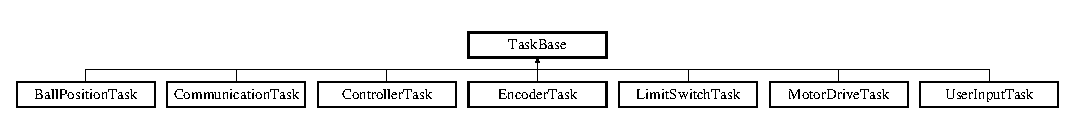
\includegraphics[height=1.221374cm]{class_task_base}
\end{center}
\end{figure}
\subsection*{Public Member Functions}
\begin{DoxyCompactItemize}
\item 
\mbox{\hyperlink{class_task_base_ae8e359a838bed17302e4f21146dba612}{Task\+Base}} (const char $\ast$a\+\_\+name, unsigned port\+B\+A\+S\+E\+\_\+\+T\+Y\+PE a\+\_\+priority=0, size\+\_\+t a\+\_\+stack\+\_\+size=config\+M\+I\+N\+I\+M\+A\+L\+\_\+\+S\+T\+A\+C\+K\+\_\+\+S\+I\+ZE, \mbox{\hyperlink{classemstream}{emstream}} $\ast$p\+\_\+ser\+\_\+dev=N\+U\+LL)
\begin{DoxyCompactList}\small\item\em Constructor which creates and initializes a task object. \end{DoxyCompactList}\item 
virtual void \mbox{\hyperlink{class_task_base_adcf6036ad9c860051ccf392ba5e7dbbc}{run}} (void)=0
\begin{DoxyCompactList}\small\item\em Run method which holds the user\textquotesingle{}s task code. \end{DoxyCompactList}\item 
void \mbox{\hyperlink{class_task_base_af70bf7c9cb6dfccdb1dbf41b7c6d2ecf}{transition\+\_\+to}} (uint8\+\_\+t)
\begin{DoxyCompactList}\small\item\em Cause this task to transition to another state. \end{DoxyCompactList}\item 
void \mbox{\hyperlink{class_task_base_ad088ca82db29301b019b1efde85156be}{set\+\_\+serial\+\_\+device}} (\mbox{\hyperlink{classemstream}{emstream}} $\ast$p\+\_\+new\+\_\+dev)
\begin{DoxyCompactList}\small\item\em Set the task\textquotesingle{}s serial device pointer. \end{DoxyCompactList}\item 
void \mbox{\hyperlink{class_task_base_a0e1cc480afef3708598b6b217b281a7b}{unset\+\_\+serial\+\_\+device}} (void)
\begin{DoxyCompactList}\small\item\em Turn off serial logging by un-\/setting the task\textquotesingle{}s serial pointer. \end{DoxyCompactList}\item 
\mbox{\hyperlink{class_task_base_a0dbf9678429543f33c9c8f82511a3887}{operator bool}} () const
\begin{DoxyCompactList}\small\item\em Check if a task is ready to run. \end{DoxyCompactList}\item 
void \mbox{\hyperlink{class_task_base_a06d9c962cc578a84a69ca637f6d5adef}{delay}} (Tick\+Type\+\_\+t duration)
\begin{DoxyCompactList}\small\item\em Stop running the task for the given number of R\+T\+OS ticks. \end{DoxyCompactList}\item 
void \mbox{\hyperlink{class_task_base_a6a7e9bc3d85a0e71462002b85402d995}{delay\+\_\+ms}} (Tick\+Type\+\_\+t duration\+\_\+ms)
\begin{DoxyCompactList}\small\item\em Stop the task for approximately the given number of milliseconds. \end{DoxyCompactList}\item 
void \mbox{\hyperlink{class_task_base_adc48db72592a8b34ca1235e1d18604cc}{delay\+\_\+from\+\_\+for}} (Tick\+Type\+\_\+t \&from\+\_\+ticks, Tick\+Type\+\_\+t for\+\_\+how\+\_\+long)
\begin{DoxyCompactList}\small\item\em Stop the task from running for a precise time interval. \end{DoxyCompactList}\item 
void \mbox{\hyperlink{class_task_base_a31b1c01059c7ec4bfe60fc8332759551}{delay\+\_\+from\+\_\+for\+\_\+ms}} (Tick\+Type\+\_\+t \&from\+\_\+ticks, Tick\+Type\+\_\+t millisec)
\begin{DoxyCompactList}\small\item\em Stop the task from running for a precise number of milliseconds. \end{DoxyCompactList}\item 
Tick\+Type\+\_\+t \mbox{\hyperlink{class_task_base_aea05d3d35f6cbda823ed4812b0951944}{get\+\_\+tick\+\_\+count}} (void)
\begin{DoxyCompactList}\small\item\em Find out how many R\+T\+OS ticks since the scheduler was started. \end{DoxyCompactList}\item 
void \mbox{\hyperlink{class_task_base_a4e9fe49dbbf245e182abf6d17c9bd3df}{yield}} (void)
\begin{DoxyCompactList}\small\item\em The task gives control to the R\+T\+OS immediately. \end{DoxyCompactList}\item 
port\+B\+A\+S\+E\+\_\+\+T\+Y\+PE \mbox{\hyperlink{class_task_base_a1f26fc9564898da36d2355095c204340}{get\+\_\+priority}} (void)
\begin{DoxyCompactList}\small\item\em Return the task\textquotesingle{}s current priority. \end{DoxyCompactList}\item 
void \mbox{\hyperlink{class_task_base_a1a6f54b0b07cf27d5764c4dca5ec5fcf}{set\+\_\+priority}} (port\+B\+A\+S\+E\+\_\+\+T\+Y\+PE new\+\_\+priority)
\begin{DoxyCompactList}\small\item\em Set this task\textquotesingle{}s priority to a new value. \end{DoxyCompactList}\item 
size\+\_\+t \mbox{\hyperlink{class_task_base_a822796dba0ef4d457608363507d65f5a}{heap\+\_\+left}} (void)
\begin{DoxyCompactList}\small\item\em Return the number of unused bytes in the heap. \end{DoxyCompactList}\item 
void \mbox{\hyperlink{class_task_base_a9e228e424048594a935cd31ae9e0eeb3}{dump\+\_\+stack}} (\mbox{\hyperlink{classemstream}{emstream}} $\ast$p\+\_\+ser\+\_\+dev)
\begin{DoxyCompactList}\small\item\em Print a display of this task\textquotesingle{}s stack space. \end{DoxyCompactList}\item 
void \mbox{\hyperlink{class_task_base_a441138caa57e35f58f31dc4d960580d9}{print\+\_\+stack\+\_\+in\+\_\+list}} (\mbox{\hyperlink{classemstream}{emstream}} $\ast$p\+\_\+ser\+\_\+dev)
\begin{DoxyCompactList}\small\item\em Print a stack dump within a dump of all tasks\textquotesingle{} stacks. \end{DoxyCompactList}\item 
size\+\_\+t \mbox{\hyperlink{class_task_base_aa3979e41ecb8f646f12d4283d87f93df}{get\+\_\+total\+\_\+stack}} (void)
\begin{DoxyCompactList}\small\item\em Return the total stack size for this task. \end{DoxyCompactList}\item 
uint8\+\_\+t \mbox{\hyperlink{class_task_base_ae4f412b0911d4cf84dad9169a10c46e0}{get\+\_\+state}} (void)
\begin{DoxyCompactList}\small\item\em Return the current state in which this task\textquotesingle{}s state machine is. \end{DoxyCompactList}\item 
float \mbox{\hyperlink{class_task_base_a4d0769068c3095d76752e0a00963d8b8}{get\+\_\+tick\+\_\+time}} (void)
\begin{DoxyCompactList}\small\item\em Return an approximate measurement of time from the tick count. \end{DoxyCompactList}\item 
const char $\ast$ \mbox{\hyperlink{class_task_base_a69b0a4031cf715d9d3a6ecd3b29f5cbe}{get\+\_\+name}} (void)
\begin{DoxyCompactList}\small\item\em Return a pointer to this task\textquotesingle{}s name. \end{DoxyCompactList}\item 
void \mbox{\hyperlink{class_task_base_a58bd479a964b4c98da9f8f1a6b08efd7}{print\+\_\+status\+\_\+in\+\_\+list}} (\mbox{\hyperlink{classemstream}{emstream}} $\ast$)
\item 
Task\+Handle\+\_\+t \mbox{\hyperlink{class_task_base_a2113de68c720fcf8b643b11a43b84ab7}{get\+\_\+handle}} (void)
\begin{DoxyCompactList}\small\item\em Return a handle to the Free\+R\+T\+OS task wrapped by this task object. \end{DoxyCompactList}\item 
virtual void \mbox{\hyperlink{class_task_base_aea504e1e3d38a7e8e8c65c4284d4a560}{print\+\_\+status}} (\mbox{\hyperlink{classemstream}{emstream}} \&)
\item 
void \mbox{\hyperlink{class_task_base_a5842a497b5a274e6a40fae18bff03a9f}{emergency\+\_\+reset}} (const char $\ast$message)
\begin{DoxyCompactList}\small\item\em Print an error message if possible and reset the processor. \end{DoxyCompactList}\end{DoxyCompactItemize}
\subsection*{Static Public Member Functions}
\begin{DoxyCompactItemize}
\item 
static void \mbox{\hyperlink{class_task_base_a9884c542600faa2f90da35c832fea87a}{\+\_\+call\+\_\+users\+\_\+run\+\_\+method}} (\mbox{\hyperlink{class_task_base}{Task\+Base}} $\ast$)
\begin{DoxyCompactList}\small\item\em Internal use only function which calls the {\ttfamily \mbox{\hyperlink{class_task_base_adcf6036ad9c860051ccf392ba5e7dbbc}{run()}}} method. \end{DoxyCompactList}\item 
static const \mbox{\hyperlink{class_task_base}{Task\+Base}} $\ast$ \mbox{\hyperlink{class_task_base_a6d6efe1287e0d4b73064af05626e48d2}{get\+\_\+last\+\_\+created\+\_\+task\+\_\+pointer}} (void)
\begin{DoxyCompactList}\small\item\em Return a pointer to the most recently created task. \end{DoxyCompactList}\end{DoxyCompactItemize}
\subsection*{Protected Member Functions}
\begin{DoxyCompactItemize}
\item 
uint32\+\_\+t \mbox{\hyperlink{class_task_base_adbc9cc6b14c5396c38457edc9c9bc215}{get\+\_\+loop\+\_\+runs}} (void)
\end{DoxyCompactItemize}
\subsection*{Protected Attributes}
\begin{DoxyCompactItemize}
\item 
\mbox{\Hypertarget{class_task_base_abd349e5f74bd10d1288459b66858ea26}\label{class_task_base_abd349e5f74bd10d1288459b66858ea26}} 
Task\+Handle\+\_\+t \mbox{\hyperlink{class_task_base_abd349e5f74bd10d1288459b66858ea26}{handle}}
\begin{DoxyCompactList}\small\item\em This is the handle of this R\+T\+OS task. It\textquotesingle{}s typedef\textquotesingle{}d as a pointer type. \end{DoxyCompactList}\item 
\mbox{\hyperlink{class_task_base}{Task\+Base}} $\ast$ \mbox{\hyperlink{class_task_base_a4f8adbe534975ada5ffb46fa403ef07f}{prev\+\_\+task\+\_\+pointer}}
\item 
\mbox{\hyperlink{classemstream}{emstream}} $\ast$ \mbox{\hyperlink{class_task_base_a5299f7fa222eb0ddac3b77e667170fd7}{p\+\_\+serial}}
\item 
uint8\+\_\+t \mbox{\hyperlink{class_task_base_aab6866bbd5d036810829ccc7cd3ab0e8}{state}}
\item 
uint8\+\_\+t \mbox{\hyperlink{class_task_base_a9736ccdb46487c91c49bdbf2c24b52d3}{previous\+\_\+state}}
\item 
uint32\+\_\+t \mbox{\hyperlink{class_task_base_ab5503939e17359f0f3f9249f622df389}{runs}}
\end{DoxyCompactItemize}


\subsection{Detailed Description}
Base class for implementations of tasks in task/state based programs. 

This class is a C++ wrapper for the Free\+R\+T\+OS task functions with some extra functionality for keeping track of state transitions and for printing diagnostic information about how tasks are configured and how they are running.\hypertarget{index_Usage}{}\subsection{Usage}\label{index_Usage}
In order to use a task, one must first create a child class of class {\ttfamily \mbox{\hyperlink{class_task_base}{Task\+Base}}}. The child class must at least have a constructor and a run method\+: 
\begin{DoxyCode}
\textcolor{keyword}{class }TaskExample : \textcolor{keyword}{public} \mbox{\hyperlink{class_task_base}{TaskBase}}
\{
\textcolor{keyword}{protected}:
    \textcolor{comment}{// Task specific data goes here}

\textcolor{keyword}{public}:
    \textcolor{comment}{// This constructor creates an example task object}
       TaskExample (\textcolor{keyword}{const} \textcolor{keywordtype}{char}*, \textcolor{keywordtype}{unsigned} portBASE\_TYPE, \textcolor{keywordtype}{size\_t}, \mbox{\hyperlink{classemstream}{emstream}}*);

    \textcolor{comment}{// This run method is called by the RTOS and contains a loop }
    \textcolor{keywordtype}{void} \mbox{\hyperlink{class_task_base_adcf6036ad9c860051ccf392ba5e7dbbc}{run}} (\textcolor{keywordtype}{void});
\};
\end{DoxyCode}


The task class\textquotesingle{}s constructor can sometimes be quite simple, only calling the parent constructor as shown in the example below\+: 
\begin{DoxyCode}
TaskExample::TaskExample (\textcolor{keyword}{const} \textcolor{keywordtype}{char}* a\_name,
                          \textcolor{keywordtype}{unsigned} portBASE\_TYPE a\_priority,
                          \textcolor{keywordtype}{size\_t} a\_stack\_size,
                          \mbox{\hyperlink{classemstream}{emstream}}* p\_serial\_dev
                         )
    : \mbox{\hyperlink{class_task_base}{TaskBase}} (a\_name, a\_priority, a\_stack\_size, p\_serial\_dev)
\{
\}
\end{DoxyCode}
 If the task needs to initialize device drivers or other things it owns, that can be done in the constructor.

Every task must have a user-\/written run method named {\ttfamily \mbox{\hyperlink{class_task_base_adcf6036ad9c860051ccf392ba5e7dbbc}{run()}}}. The run method is where most of the functionality of the task is implemented. The run method must contain an endless loop in which the task\textquotesingle{}s state machine is implemented. A variable called {\ttfamily state} is kept by the parent class {\ttfamily \mbox{\hyperlink{class_task_base}{Task\+Base}}} and used to monitor the state in which the user\textquotesingle{}s code is running, so one should {\bfseries not} declare another variable called {\ttfamily state} inside the run method\+: 
\begin{DoxyCode}
\textcolor{keywordtype}{void} TaskExample::run (\textcolor{keywordtype}{void})
\{
    TickType\_t LastWakeTime;                   \textcolor{comment}{// For scheduling how often task runs}

    \textcolor{comment}{// Initialise the LastWakeTime variable with the current time. This happens just}
    \textcolor{comment}{// once, before the infinite loop is entered}
       LastWakeTime = \mbox{\hyperlink{class_task_base_aea05d3d35f6cbda823ed4812b0951944}{get\_tick\_count}} ();

    \textcolor{comment}{// This is the task loop. Once the task has been initialized in the code just}
    \textcolor{comment}{// above, the task loop runs, and it keeps running until the power is shut off}
    \textcolor{keywordflow}{for} (;;)
    \{
        \textcolor{comment}{// Run the task's state machine here}
        \textcolor{keywordflow}{switch} (\mbox{\hyperlink{class_task_base_aab6866bbd5d036810829ccc7cd3ab0e8}{state}})
        \{
            \textcolor{keywordflow}{case} 0:
                \textcolor{comment}{// Do one thing in State 0}
                ...
                \textcolor{comment}{// Check for a transition to another state}
                \textcolor{keywordflow}{if} (something)
                \{
                    \mbox{\hyperlink{class_task_base_af70bf7c9cb6dfccdb1dbf41b7c6d2ecf}{transition\_to}} (1);
                \}
                \textcolor{keywordflow}{break};

            \textcolor{keywordflow}{case} 1:
                \textcolor{comment}{// Do another thing in State 1}
                ...
                \textcolor{keywordflow}{break};

            \textcolor{keywordflow}{case} 2:
                \textcolor{comment}{// Do something completely different in State 2}
                ...
                \textcolor{keywordflow}{break};
        \};

        \textcolor{comment}{// Tell the RTOS to delay until the given number of RTOS timer ticks have}
        \textcolor{comment}{// elapsed. This means the code after this line runs every ticks\_per\_run}
        \textcolor{comment}{// milliseconds if the RTOS interrupt is set to go off every 1 millisecond}
        \mbox{\hyperlink{class_task_base_adc48db72592a8b34ca1235e1d18604cc}{delay\_from\_for}} (LastWakeTime, ticks\_per\_run);
    \}
\}
\end{DoxyCode}


Tasks are traditionally instantiated within {\ttfamily \mbox{\hyperlink{main_8cpp_a840291bc02cba5474a4cb46a9b9566fe}{main()}}}. The most important and tricky part about creating a task is getting its {\bfseries stack} size right. If a task\textquotesingle{}s stack is too large, it will waste R\+AM, and small microcontrollers don\textquotesingle{}t have much R\+AM to waste. If the task\textquotesingle{}s stack is too small, it will cause disaster, usually in the form of the processor either hanging or rebooting as the stack pointer for the task goes outside the allocated range and overwrites the stack for another task. For Free\+R\+T\+OS tasks on an 8-\/bit A\+VR microcontroller, the smallest stack size that is likely to ever work is about 100 bytes. As soon as data is created within the run method, queues are used, and other memory is used, the necessary stack size goes up; it is common to need 300 -- 500 bytes of stack space for a task that does a lot of work. Because it\textquotesingle{}s very difficult to calculate the stack space needed for a task, the easiest way to set the stack size is usually to make it large enough that the program runs reliably, then decrease it by about 20 bytes at a time, recompile and test the program, again and again until something fails. Then make the stack size a couple dozen bytes larger than the smallest size that reliably worked during testing...just in case.

The code used to create a task object looks like the following\+: 
\begin{DoxyCode}
\textcolor{comment}{// Create an example task. It runs at priority 2 and has a 200 byte stack}
TaskExample* my\_example\_task 
    = \textcolor{keyword}{new} TaskExample (\textcolor{stringliteral}{"Example"}, tskIDLE\_PRIORITY + 2, 200, &ser\_port);
...
\textcolor{comment}{// Start up the scheduler, causing all tasks to be run}
vTaskStartScheduler ();
\end{DoxyCode}
 In this example code, someone must have created the serial port object named {\ttfamily ser\+\_\+port} previously; the serial port will be used by the task to print out diagnostic information. If no diagnostic information needs to be printed, the serial port may be left out of the task constructor call or set to {\ttfamily N\+U\+LL}. 

\subsection{Constructor \& Destructor Documentation}
\mbox{\Hypertarget{class_task_base_ae8e359a838bed17302e4f21146dba612}\label{class_task_base_ae8e359a838bed17302e4f21146dba612}} 
\index{Task\+Base@{Task\+Base}!Task\+Base@{Task\+Base}}
\index{Task\+Base@{Task\+Base}!Task\+Base@{Task\+Base}}
\subsubsection{\texorpdfstring{Task\+Base()}{TaskBase()}}
{\footnotesize\ttfamily Task\+Base\+::\+Task\+Base (\begin{DoxyParamCaption}\item[{const char $\ast$}]{a\+\_\+name,  }\item[{unsigned port\+B\+A\+S\+E\+\_\+\+T\+Y\+PE}]{a\+\_\+priority = {\ttfamily 0},  }\item[{size\+\_\+t}]{a\+\_\+stack\+\_\+size = {\ttfamily configMINIMAL\+\_\+STACK\+\_\+SIZE},  }\item[{\mbox{\hyperlink{classemstream}{emstream}} $\ast$}]{p\+\_\+ser\+\_\+dev = {\ttfamily NULL} }\end{DoxyParamCaption})\hspace{0.3cm}{\ttfamily [explicit]}}



Constructor which creates and initializes a task object. 

This constructor creates a Free\+R\+T\+OS task with the given task run function, name, priority, and stack size. It saves a pointers to a serial device to be used for debugging; it also saves a pointer to the previously created task (if any) so that tasks can form a linked list. Any function, such as diagnostic printouts, that is to be performed by all tasks can be done by telling the most recently created task to do it, then have that most recently created task tell the previously created task to do it, and so on.

The odd parameter with the {\ttfamily reinterpret\+\_\+cast} directive is a pointer to the Free\+R\+T\+OS task run function. This pointer, which is supplied to Free\+R\+T\+OS as a pointer to a function that takes one void pointer parameter and returns nothing, contains a reference to a method belonging to this class called {\bfseries \mbox{\hyperlink{taskbase_8cpp_abeff30a44eadf95fa24c7215cc6d7eae}{\+\_\+call\+\_\+static\+\_\+run\+\_\+method()}}}. Free\+R\+T\+OS will then call {\bfseries \mbox{\hyperlink{taskbase_8cpp_abeff30a44eadf95fa24c7215cc6d7eae}{\+\_\+call\+\_\+static\+\_\+run\+\_\+method()}}} which is a regular C (not C++) function that is given a pointer to the task object which the user has created. {\bfseries \mbox{\hyperlink{taskbase_8cpp_abeff30a44eadf95fa24c7215cc6d7eae}{\+\_\+call\+\_\+static\+\_\+run\+\_\+method()}}}, being a member of this class, then calls the user\textquotesingle{}s {\bfseries \mbox{\hyperlink{class_task_base_adcf6036ad9c860051ccf392ba5e7dbbc}{run()}}} method using the fancy virtual method function finding tricks that it can use because it is a C++ method rather than a plain old C function. All this C++ and virtual method fanciness only has to take place once as the scheduler is starting up, so it doesn\textquotesingle{}t slow real-\/time operation down. 
\begin{DoxyParams}{Parameters}
{\em a\+\_\+name} & A character string which will be the name of this task \\
\hline
{\em a\+\_\+priority} & The priority at which this task will initially run (default\+: 0) \\
\hline
{\em a\+\_\+stack\+\_\+size} & The size of this task\textquotesingle{}s stack in bytes (default\+: {\ttfamily config\+M\+I\+N\+I\+M\+A\+L\+\_\+\+S\+T\+A\+C\+K\+\_\+\+S\+I\+ZE}) \\
\hline
{\em p\+\_\+ser\+\_\+dev} & Pointer to a serial device (port, radio, SD card, etc.) which can be used by this task to communicate (default\+: N\+U\+LL) \\
\hline
\end{DoxyParams}


\subsection{Member Function Documentation}
\mbox{\Hypertarget{class_task_base_a9884c542600faa2f90da35c832fea87a}\label{class_task_base_a9884c542600faa2f90da35c832fea87a}} 
\index{Task\+Base@{Task\+Base}!\+\_\+call\+\_\+users\+\_\+run\+\_\+method@{\+\_\+call\+\_\+users\+\_\+run\+\_\+method}}
\index{\+\_\+call\+\_\+users\+\_\+run\+\_\+method@{\+\_\+call\+\_\+users\+\_\+run\+\_\+method}!Task\+Base@{Task\+Base}}
\subsubsection{\texorpdfstring{\+\_\+call\+\_\+users\+\_\+run\+\_\+method()}{\_call\_users\_run\_method()}}
{\footnotesize\ttfamily void Task\+Base\+::\+\_\+call\+\_\+users\+\_\+run\+\_\+method (\begin{DoxyParamCaption}\item[{\mbox{\hyperlink{class_task_base}{Task\+Base}} $\ast$}]{p\+\_\+task }\end{DoxyParamCaption})\hspace{0.3cm}{\ttfamily [static]}}



Internal use only function which calls the {\ttfamily \mbox{\hyperlink{class_task_base_adcf6036ad9c860051ccf392ba5e7dbbc}{run()}}} method. 

{\bfseries This method never needs to be called by user-\/written code.} This {\ttfamily static} method calls the user-\/written {\ttfamily \mbox{\hyperlink{class_task_base_adcf6036ad9c860051ccf392ba5e7dbbc}{run()}}} method when it has been called by {\ttfamily \mbox{\hyperlink{taskbase_8cpp_abeff30a44eadf95fa24c7215cc6d7eae}{\+\_\+call\+\_\+static\+\_\+run\+\_\+method()}}}. The function {\ttfamily \mbox{\hyperlink{taskbase_8cpp_abeff30a44eadf95fa24c7215cc6d7eae}{\+\_\+call\+\_\+static\+\_\+run\+\_\+method()}}} function was, in turn, called by Free\+R\+T\+OS; it is the C (not C++) function which was registered with the scheduler. 
\begin{DoxyParams}{Parameters}
{\em p\+\_\+task} & A pointer to the task (this task) whose run method is to be called \\
\hline
\end{DoxyParams}
\mbox{\Hypertarget{class_task_base_a06d9c962cc578a84a69ca637f6d5adef}\label{class_task_base_a06d9c962cc578a84a69ca637f6d5adef}} 
\index{Task\+Base@{Task\+Base}!delay@{delay}}
\index{delay@{delay}!Task\+Base@{Task\+Base}}
\subsubsection{\texorpdfstring{delay()}{delay()}}
{\footnotesize\ttfamily void Task\+Base\+::delay (\begin{DoxyParamCaption}\item[{Tick\+Type\+\_\+t}]{duration }\end{DoxyParamCaption})\hspace{0.3cm}{\ttfamily [inline]}}



Stop running the task for the given number of R\+T\+OS ticks. 

This method causes the task to stop running for the given number of R\+T\+OS ticks from the time it is called. This method should {\bfseries not} be used to make a task run at regular intervals, because the time between when the previous delay ended and and when {\ttfamily \mbox{\hyperlink{class_task_base_a06d9c962cc578a84a69ca637f6d5adef}{delay()}}} is called subsequently can vary, leading to the accumulation of errors in timing. For periodic runs of code in a task, see {\ttfamily \mbox{\hyperlink{class_task_base_adc48db72592a8b34ca1235e1d18604cc}{delay\+\_\+from\+\_\+for()}}}. 
\begin{DoxyParams}{Parameters}
{\em duration} & The amount of time, as a number of timer ticks, this task should wait until next running \\
\hline
\end{DoxyParams}
\mbox{\Hypertarget{class_task_base_adc48db72592a8b34ca1235e1d18604cc}\label{class_task_base_adc48db72592a8b34ca1235e1d18604cc}} 
\index{Task\+Base@{Task\+Base}!delay\+\_\+from\+\_\+for@{delay\+\_\+from\+\_\+for}}
\index{delay\+\_\+from\+\_\+for@{delay\+\_\+from\+\_\+for}!Task\+Base@{Task\+Base}}
\subsubsection{\texorpdfstring{delay\+\_\+from\+\_\+for()}{delay\_from\_for()}}
{\footnotesize\ttfamily void Task\+Base\+::delay\+\_\+from\+\_\+for (\begin{DoxyParamCaption}\item[{Tick\+Type\+\_\+t \&}]{from\+\_\+ticks,  }\item[{Tick\+Type\+\_\+t}]{for\+\_\+how\+\_\+long }\end{DoxyParamCaption})\hspace{0.3cm}{\ttfamily [inline]}}



Stop the task from running for a precise time interval. 

This method causes the task to stop running from a given time for a specified duration. The start time and duration are given in units of R\+T\+OS timer ticks. This method can be used to implement a task that regularly wakes up and performs some action, like a clown waking up to terrify children. Because the time at which each awakening takes place is recorded, this method won\textquotesingle{}t accumulate errors as it is repeatedly invoked. 
\begin{DoxyParams}{Parameters}
{\em from\+\_\+ticks} & The beginning time of the duration to delay. It is usually set equal to the time at which the previous delay began so as to get precise, regular timing \\
\hline
{\em for\+\_\+how\+\_\+long} & The duration of the delay interval in R\+T\+OS ticks \\
\hline
\end{DoxyParams}
\mbox{\Hypertarget{class_task_base_a31b1c01059c7ec4bfe60fc8332759551}\label{class_task_base_a31b1c01059c7ec4bfe60fc8332759551}} 
\index{Task\+Base@{Task\+Base}!delay\+\_\+from\+\_\+for\+\_\+ms@{delay\+\_\+from\+\_\+for\+\_\+ms}}
\index{delay\+\_\+from\+\_\+for\+\_\+ms@{delay\+\_\+from\+\_\+for\+\_\+ms}!Task\+Base@{Task\+Base}}
\subsubsection{\texorpdfstring{delay\+\_\+from\+\_\+for\+\_\+ms()}{delay\_from\_for\_ms()}}
{\footnotesize\ttfamily void Task\+Base\+::delay\+\_\+from\+\_\+for\+\_\+ms (\begin{DoxyParamCaption}\item[{Tick\+Type\+\_\+t \&}]{from\+\_\+ticks,  }\item[{Tick\+Type\+\_\+t}]{millisec }\end{DoxyParamCaption})\hspace{0.3cm}{\ttfamily [inline]}}



Stop the task from running for a precise number of milliseconds. 

This method causes the task to delay from a given time for a specified duration in milliseconds. This is usually done to make a task that runs code at a fairly precise and regular interval. The start time is given in units of R\+T\+OS timer ticks; although ticks might not equal milliseconds, the user need not care, just store the value in a variable of type {\ttfamily Tick\+Type\+\_\+t}. The delay duration is given in milliseconds. An example of how this method is used follows\+: 
\begin{DoxyCode}
\textcolor{comment}{// Make a variable which will hold tick counts and initialize it}
TickType\_t previousTicks = xTaskGetTickCount ();
...
for (;;)                   \textcolor{comment}{// The task loop}
\{
    ...                    \textcolor{comment}{// User code to run every 10 ms}
    ...
    \mbox{\hyperlink{class_task_base_a31b1c01059c7ec4bfe60fc8332759551}{delay\_from\_for\_ms}} (previousTicks, 10);
\}
\end{DoxyCode}
 {\bfseries Warning\+:} In order for this function to provide accurate timing, the R\+T\+OS tick rate (set in {\ttfamily \mbox{\hyperlink{_free_r_t_o_s_config_8h_source}{Free\+R\+T\+O\+S\+Config.\+h}}} ) must be set to a rate such that R\+T\+OS ticks occur at the desired time interval. For example, if a task must awaken once per millisecond, ticks at 1 ms or 0.\+5 ms are OK, but ticks every 2 ms or 0.\+7 ms will not allow pricise timing. 
\begin{DoxyParams}{Parameters}
{\em from\+\_\+ticks} & The beginning time of the duration to delay. It is usually set equal to the end time of the previous delay so as to get precise, regular timing \\
\hline
{\em millisec} & The duration of the delay interval in milliseconds \\
\hline
\end{DoxyParams}
\mbox{\Hypertarget{class_task_base_a6a7e9bc3d85a0e71462002b85402d995}\label{class_task_base_a6a7e9bc3d85a0e71462002b85402d995}} 
\index{Task\+Base@{Task\+Base}!delay\+\_\+ms@{delay\+\_\+ms}}
\index{delay\+\_\+ms@{delay\+\_\+ms}!Task\+Base@{Task\+Base}}
\subsubsection{\texorpdfstring{delay\+\_\+ms()}{delay\_ms()}}
{\footnotesize\ttfamily void Task\+Base\+::delay\+\_\+ms (\begin{DoxyParamCaption}\item[{Tick\+Type\+\_\+t}]{duration\+\_\+ms }\end{DoxyParamCaption})\hspace{0.3cm}{\ttfamily [inline]}}



Stop the task for approximately the given number of milliseconds. 

This method causes the task to stop running for approximately the given number of milliseconds. This method should {\bfseries not} be used to make a task run at regular intervals, because the time between when the previous delay ended and and when {\ttfamily \mbox{\hyperlink{class_task_base_a6a7e9bc3d85a0e71462002b85402d995}{delay\+\_\+ms()}}} is called subsequently can vary, leading to the accumulation of errors in timing. For periodic runs of code in a task, see {\ttfamily \mbox{\hyperlink{class_task_base_a31b1c01059c7ec4bfe60fc8332759551}{delay\+\_\+from\+\_\+for\+\_\+ms()}}}. 
\begin{DoxyParams}{Parameters}
{\em duration\+\_\+ms} & The duration for the task to stop in milliseconds \\
\hline
\end{DoxyParams}
\mbox{\Hypertarget{class_task_base_a9e228e424048594a935cd31ae9e0eeb3}\label{class_task_base_a9e228e424048594a935cd31ae9e0eeb3}} 
\index{Task\+Base@{Task\+Base}!dump\+\_\+stack@{dump\+\_\+stack}}
\index{dump\+\_\+stack@{dump\+\_\+stack}!Task\+Base@{Task\+Base}}
\subsubsection{\texorpdfstring{dump\+\_\+stack()}{dump\_stack()}}
{\footnotesize\ttfamily void Task\+Base\+::dump\+\_\+stack (\begin{DoxyParamCaption}\item[{\mbox{\hyperlink{classemstream}{emstream}} $\ast$}]{p\+\_\+ser\+\_\+dev }\end{DoxyParamCaption})\hspace{0.3cm}{\ttfamily [inline]}}



Print a display of this task\textquotesingle{}s stack space. 

This method prints a hexadecimal and text format dump of the stack\textquotesingle{}s contents for debugging and instructional purposes. 
\begin{DoxyParams}{Parameters}
{\em p\+\_\+ser\+\_\+dev} & The serial device to which the stack will be printed \\
\hline
\end{DoxyParams}
\mbox{\Hypertarget{class_task_base_a5842a497b5a274e6a40fae18bff03a9f}\label{class_task_base_a5842a497b5a274e6a40fae18bff03a9f}} 
\index{Task\+Base@{Task\+Base}!emergency\+\_\+reset@{emergency\+\_\+reset}}
\index{emergency\+\_\+reset@{emergency\+\_\+reset}!Task\+Base@{Task\+Base}}
\subsubsection{\texorpdfstring{emergency\+\_\+reset()}{emergency\_reset()}}
{\footnotesize\ttfamily void Task\+Base\+::emergency\+\_\+reset (\begin{DoxyParamCaption}\item[{const char $\ast$}]{message }\end{DoxyParamCaption})}



Print an error message if possible and reset the processor. 

This method prints an error message (if there is a valid serial device pointer available) and resets the processor. It should only be used in cases of things going seriously to heck. 
\begin{DoxyParams}{Parameters}
{\em message} & A message to print before restarting; {\ttfamily endl} is appended to it \\
\hline
\end{DoxyParams}
\mbox{\Hypertarget{class_task_base_a2113de68c720fcf8b643b11a43b84ab7}\label{class_task_base_a2113de68c720fcf8b643b11a43b84ab7}} 
\index{Task\+Base@{Task\+Base}!get\+\_\+handle@{get\+\_\+handle}}
\index{get\+\_\+handle@{get\+\_\+handle}!Task\+Base@{Task\+Base}}
\subsubsection{\texorpdfstring{get\+\_\+handle()}{get\_handle()}}
{\footnotesize\ttfamily Task\+Handle\+\_\+t Task\+Base\+::get\+\_\+handle (\begin{DoxyParamCaption}\item[{void}]{ }\end{DoxyParamCaption})\hspace{0.3cm}{\ttfamily [inline]}}



Return a handle to the Free\+R\+T\+OS task wrapped by this task object. 

This method returns the handle of the Free\+R\+T\+OS task which is inside this object. Advanced users might want to use it to access task manipulation functions that aren\textquotesingle{}t in this wrapper class or for other creative hacking. \begin{DoxyReturn}{Returns}
The handle of the Free\+R\+T\+OS task which is wrapped in this handy C++ class 
\end{DoxyReturn}
\mbox{\Hypertarget{class_task_base_a6d6efe1287e0d4b73064af05626e48d2}\label{class_task_base_a6d6efe1287e0d4b73064af05626e48d2}} 
\index{Task\+Base@{Task\+Base}!get\+\_\+last\+\_\+created\+\_\+task\+\_\+pointer@{get\+\_\+last\+\_\+created\+\_\+task\+\_\+pointer}}
\index{get\+\_\+last\+\_\+created\+\_\+task\+\_\+pointer@{get\+\_\+last\+\_\+created\+\_\+task\+\_\+pointer}!Task\+Base@{Task\+Base}}
\subsubsection{\texorpdfstring{get\+\_\+last\+\_\+created\+\_\+task\+\_\+pointer()}{get\_last\_created\_task\_pointer()}}
{\footnotesize\ttfamily static const \mbox{\hyperlink{class_task_base}{Task\+Base}}$\ast$ Task\+Base\+::get\+\_\+last\+\_\+created\+\_\+task\+\_\+pointer (\begin{DoxyParamCaption}\item[{void}]{ }\end{DoxyParamCaption})\hspace{0.3cm}{\ttfamily [inline]}, {\ttfamily [static]}}



Return a pointer to the most recently created task. 

This method returns a pointer to the most recently created task. This pointer is the head of a linked list of tasks; the list is maintained by the task objects themselves. This pointer to the most recently created task is used to begin traversing the list of all tasks when some action needs to be taken by all the tasks. \begin{DoxyReturn}{Returns}
A pointer to the most recently created task 
\end{DoxyReturn}
\mbox{\Hypertarget{class_task_base_adbc9cc6b14c5396c38457edc9c9bc215}\label{class_task_base_adbc9cc6b14c5396c38457edc9c9bc215}} 
\index{Task\+Base@{Task\+Base}!get\+\_\+loop\+\_\+runs@{get\+\_\+loop\+\_\+runs}}
\index{get\+\_\+loop\+\_\+runs@{get\+\_\+loop\+\_\+runs}!Task\+Base@{Task\+Base}}
\subsubsection{\texorpdfstring{get\+\_\+loop\+\_\+runs()}{get\_loop\_runs()}}
{\footnotesize\ttfamily uint32\+\_\+t Task\+Base\+::get\+\_\+loop\+\_\+runs (\begin{DoxyParamCaption}\item[{void}]{ }\end{DoxyParamCaption})\hspace{0.3cm}{\ttfamily [inline]}, {\ttfamily [protected]}}

This method allows descendent classes to find out how many times the {\ttfamily loop()} method has run. \begin{DoxyReturn}{Returns}
The number of times the loop has been run 
\end{DoxyReturn}
\mbox{\Hypertarget{class_task_base_a69b0a4031cf715d9d3a6ecd3b29f5cbe}\label{class_task_base_a69b0a4031cf715d9d3a6ecd3b29f5cbe}} 
\index{Task\+Base@{Task\+Base}!get\+\_\+name@{get\+\_\+name}}
\index{get\+\_\+name@{get\+\_\+name}!Task\+Base@{Task\+Base}}
\subsubsection{\texorpdfstring{get\+\_\+name()}{get\_name()}}
{\footnotesize\ttfamily const char$\ast$ Task\+Base\+::get\+\_\+name (\begin{DoxyParamCaption}\item[{void}]{ }\end{DoxyParamCaption})\hspace{0.3cm}{\ttfamily [inline]}}



Return a pointer to this task\textquotesingle{}s name. 

This method returns a pointer to the task\textquotesingle{}s name, which resides in a null terminated character array belonging to the task. Because the pointer is of type {\ttfamily const} {\ttfamily char}, that pointer cannot be used to change the task\textquotesingle{}s name (unless typecasting tricks are used in a way that is poor programming practice). \begin{DoxyReturn}{Returns}
A pointer to the task\textquotesingle{}s name 
\end{DoxyReturn}
\mbox{\Hypertarget{class_task_base_a1f26fc9564898da36d2355095c204340}\label{class_task_base_a1f26fc9564898da36d2355095c204340}} 
\index{Task\+Base@{Task\+Base}!get\+\_\+priority@{get\+\_\+priority}}
\index{get\+\_\+priority@{get\+\_\+priority}!Task\+Base@{Task\+Base}}
\subsubsection{\texorpdfstring{get\+\_\+priority()}{get\_priority()}}
{\footnotesize\ttfamily port\+B\+A\+S\+E\+\_\+\+T\+Y\+PE Task\+Base\+::get\+\_\+priority (\begin{DoxyParamCaption}\item[{void}]{ }\end{DoxyParamCaption})\hspace{0.3cm}{\ttfamily [inline]}}



Return the task\textquotesingle{}s current priority. 

\begin{DoxyReturn}{Returns}
The priority at which the task is currently running 
\end{DoxyReturn}
\mbox{\Hypertarget{class_task_base_ae4f412b0911d4cf84dad9169a10c46e0}\label{class_task_base_ae4f412b0911d4cf84dad9169a10c46e0}} 
\index{Task\+Base@{Task\+Base}!get\+\_\+state@{get\+\_\+state}}
\index{get\+\_\+state@{get\+\_\+state}!Task\+Base@{Task\+Base}}
\subsubsection{\texorpdfstring{get\+\_\+state()}{get\_state()}}
{\footnotesize\ttfamily uint8\+\_\+t Task\+Base\+::get\+\_\+state (\begin{DoxyParamCaption}\item[{void}]{ }\end{DoxyParamCaption})\hspace{0.3cm}{\ttfamily [inline]}}



Return the current state in which this task\textquotesingle{}s state machine is. 

This method returns the transition logic state in which the task is at the current time. This is the value of the variable {\ttfamily state} which is manipulated by the user within the {\ttfamily \mbox{\hyperlink{class_task_base_adcf6036ad9c860051ccf392ba5e7dbbc}{run()}}} method to cause state transitions. \begin{DoxyReturn}{Returns}
The current state 
\end{DoxyReturn}
\mbox{\Hypertarget{class_task_base_aea05d3d35f6cbda823ed4812b0951944}\label{class_task_base_aea05d3d35f6cbda823ed4812b0951944}} 
\index{Task\+Base@{Task\+Base}!get\+\_\+tick\+\_\+count@{get\+\_\+tick\+\_\+count}}
\index{get\+\_\+tick\+\_\+count@{get\+\_\+tick\+\_\+count}!Task\+Base@{Task\+Base}}
\subsubsection{\texorpdfstring{get\+\_\+tick\+\_\+count()}{get\_tick\_count()}}
{\footnotesize\ttfamily Tick\+Type\+\_\+t Task\+Base\+::get\+\_\+tick\+\_\+count (\begin{DoxyParamCaption}\item[{void}]{ }\end{DoxyParamCaption})\hspace{0.3cm}{\ttfamily [inline]}}



Find out how many R\+T\+OS ticks since the scheduler was started. 

This method returns the number of R\+T\+OS ticks from the time the scheduler was started up until the time the method is called. By using the number of R\+T\+OS ticks per second, one can determine real time approximately. The precision of this method of timekeeping isn\textquotesingle{}t really good because R\+T\+OS ticks typically only occur every millisecond or so; for high precision timing one needs to use a timer/counter running much faster than that. \begin{DoxyReturn}{Returns}
The number of R\+T\+OS ticks which have happened since R\+T\+OS startup 
\end{DoxyReturn}
\mbox{\Hypertarget{class_task_base_a4d0769068c3095d76752e0a00963d8b8}\label{class_task_base_a4d0769068c3095d76752e0a00963d8b8}} 
\index{Task\+Base@{Task\+Base}!get\+\_\+tick\+\_\+time@{get\+\_\+tick\+\_\+time}}
\index{get\+\_\+tick\+\_\+time@{get\+\_\+tick\+\_\+time}!Task\+Base@{Task\+Base}}
\subsubsection{\texorpdfstring{get\+\_\+tick\+\_\+time()}{get\_tick\_time()}}
{\footnotesize\ttfamily float Task\+Base\+::get\+\_\+tick\+\_\+time (\begin{DoxyParamCaption}\item[{void}]{ }\end{DoxyParamCaption})\hspace{0.3cm}{\ttfamily [inline]}}



Return an approximate measurement of time from the tick count. 

This method gets the tick count, which is the number of R\+T\+OS ticks which have occurred since the R\+T\+OS was started up, and converts the value from ticks into seconds. The resolution of this time measurement is only as good as the resolution of the R\+T\+OS tick rate, typically around a millisecond or so. \begin{DoxyReturn}{Returns}
The approximate real time 
\end{DoxyReturn}
\mbox{\Hypertarget{class_task_base_aa3979e41ecb8f646f12d4283d87f93df}\label{class_task_base_aa3979e41ecb8f646f12d4283d87f93df}} 
\index{Task\+Base@{Task\+Base}!get\+\_\+total\+\_\+stack@{get\+\_\+total\+\_\+stack}}
\index{get\+\_\+total\+\_\+stack@{get\+\_\+total\+\_\+stack}!Task\+Base@{Task\+Base}}
\subsubsection{\texorpdfstring{get\+\_\+total\+\_\+stack()}{get\_total\_stack()}}
{\footnotesize\ttfamily size\+\_\+t Task\+Base\+::get\+\_\+total\+\_\+stack (\begin{DoxyParamCaption}\item[{void}]{ }\end{DoxyParamCaption})\hspace{0.3cm}{\ttfamily [inline]}}



Return the total stack size for this task. 

This method returns the task\textquotesingle{}s total stack size, which was set in the constructor call. \begin{DoxyReturn}{Returns}
The task\textquotesingle{}s total stack size in bytes 
\end{DoxyReturn}
\mbox{\Hypertarget{class_task_base_a822796dba0ef4d457608363507d65f5a}\label{class_task_base_a822796dba0ef4d457608363507d65f5a}} 
\index{Task\+Base@{Task\+Base}!heap\+\_\+left@{heap\+\_\+left}}
\index{heap\+\_\+left@{heap\+\_\+left}!Task\+Base@{Task\+Base}}
\subsubsection{\texorpdfstring{heap\+\_\+left()}{heap\_left()}}
{\footnotesize\ttfamily size\+\_\+t Task\+Base\+::heap\+\_\+left (\begin{DoxyParamCaption}\item[{void}]{ }\end{DoxyParamCaption})\hspace{0.3cm}{\ttfamily [inline]}}



Return the number of unused bytes in the heap. 

This method returns the number of bytes left to be used in the heap. This means that the number returned is how many bytes available for allocation. \begin{DoxyReturn}{Returns}
The approximate number of bytes left for use in the heap 
\end{DoxyReturn}
\mbox{\Hypertarget{class_task_base_a0dbf9678429543f33c9c8f82511a3887}\label{class_task_base_a0dbf9678429543f33c9c8f82511a3887}} 
\index{Task\+Base@{Task\+Base}!operator bool@{operator bool}}
\index{operator bool@{operator bool}!Task\+Base@{Task\+Base}}
\subsubsection{\texorpdfstring{operator bool()}{operator bool()}}
{\footnotesize\ttfamily Task\+Base\+::operator \mbox{\hyperlink{group___motor___boolean___type_ga0ecf26b576b9a54eca656b9be7ba6a06}{bool}} (\begin{DoxyParamCaption}{ }\end{DoxyParamCaption}) const\hspace{0.3cm}{\ttfamily [inline]}}



Check if a task is ready to run. 

This overloaded operator allows one to check if the task is valid and ready to run. It looks at the task\textquotesingle{}s handle, which is nonzero if the task has been successfully created and hasn\textquotesingle{}t been stopped. \begin{DoxyReturn}{Returns}
True if the task has a valid R\+T\+OS task handle and false if not 
\end{DoxyReturn}
\mbox{\Hypertarget{class_task_base_a441138caa57e35f58f31dc4d960580d9}\label{class_task_base_a441138caa57e35f58f31dc4d960580d9}} 
\index{Task\+Base@{Task\+Base}!print\+\_\+stack\+\_\+in\+\_\+list@{print\+\_\+stack\+\_\+in\+\_\+list}}
\index{print\+\_\+stack\+\_\+in\+\_\+list@{print\+\_\+stack\+\_\+in\+\_\+list}!Task\+Base@{Task\+Base}}
\subsubsection{\texorpdfstring{print\+\_\+stack\+\_\+in\+\_\+list()}{print\_stack\_in\_list()}}
{\footnotesize\ttfamily void Task\+Base\+::print\+\_\+stack\+\_\+in\+\_\+list (\begin{DoxyParamCaption}\item[{\mbox{\hyperlink{classemstream}{emstream}} $\ast$}]{p\+\_\+ser\+\_\+dev }\end{DoxyParamCaption})}



Print a stack dump within a dump of all tasks\textquotesingle{} stacks. 

Show one task\textquotesingle{}s stack as a hex dump.

This method prints a stack dump, then asks the next task in the linked list of tasks to do the same, and so on and so on, so all the tasks have shown their stack space. 
\begin{DoxyParams}{Parameters}
{\em p\+\_\+ser\+\_\+dev} & A pointer to a serial device on which the stack is shown\\
\hline
\end{DoxyParams}
This method displays the task\textquotesingle{}s stack in the format of a hex dump, with the data in the stack shown as a bunch of hexadecimal numbers as well as text. Then it finds the previously created task and asks that task to print its stack as well; when the process is done all tasks (except the idle task) will have printed their stacks. The idle task\textquotesingle{}s stack is printed separately afterwards. 
\begin{DoxyParams}{Parameters}
{\em p\+\_\+ser\+\_\+dev} & The serial device to which each task prints its stack \\
\hline
\end{DoxyParams}
\mbox{\Hypertarget{class_task_base_aea504e1e3d38a7e8e8c65c4284d4a560}\label{class_task_base_aea504e1e3d38a7e8e8c65c4284d4a560}} 
\index{Task\+Base@{Task\+Base}!print\+\_\+status@{print\+\_\+status}}
\index{print\+\_\+status@{print\+\_\+status}!Task\+Base@{Task\+Base}}
\subsubsection{\texorpdfstring{print\+\_\+status()}{print\_status()}}
{\footnotesize\ttfamily void Task\+Base\+::print\+\_\+status (\begin{DoxyParamCaption}\item[{\mbox{\hyperlink{classemstream}{emstream}} \&}]{ser\+\_\+dev }\end{DoxyParamCaption})\hspace{0.3cm}{\ttfamily [virtual]}}

This method prints information about the task. It is called by the overloaded \char`\"{}$<$$<$\char`\"{} operator which is used by the task to print itself when asked to. This function is declared virtual so that descendents can override it to print additional information. 
\begin{DoxyParams}{Parameters}
{\em ser\+\_\+dev} & A reference to the serial device to which to print the task status \\
\hline
\end{DoxyParams}
\mbox{\Hypertarget{class_task_base_a58bd479a964b4c98da9f8f1a6b08efd7}\label{class_task_base_a58bd479a964b4c98da9f8f1a6b08efd7}} 
\index{Task\+Base@{Task\+Base}!print\+\_\+status\+\_\+in\+\_\+list@{print\+\_\+status\+\_\+in\+\_\+list}}
\index{print\+\_\+status\+\_\+in\+\_\+list@{print\+\_\+status\+\_\+in\+\_\+list}!Task\+Base@{Task\+Base}}
\subsubsection{\texorpdfstring{print\+\_\+status\+\_\+in\+\_\+list()}{print\_status\_in\_list()}}
{\footnotesize\ttfamily void Task\+Base\+::print\+\_\+status\+\_\+in\+\_\+list (\begin{DoxyParamCaption}\item[{\mbox{\hyperlink{classemstream}{emstream}} $\ast$}]{ser\+\_\+device }\end{DoxyParamCaption})}

This method prints task status information, then asks the next task in the list of tasks to do so. The list is kept by the tasks, each having a pointer to another. 
\begin{DoxyParams}{Parameters}
{\em ser\+\_\+device} & The serial device to which each task prints its status \\
\hline
\end{DoxyParams}
\mbox{\Hypertarget{class_task_base_adcf6036ad9c860051ccf392ba5e7dbbc}\label{class_task_base_adcf6036ad9c860051ccf392ba5e7dbbc}} 
\index{Task\+Base@{Task\+Base}!run@{run}}
\index{run@{run}!Task\+Base@{Task\+Base}}
\subsubsection{\texorpdfstring{run()}{run()}}
{\footnotesize\ttfamily virtual void Task\+Base\+::run (\begin{DoxyParamCaption}\item[{void}]{ }\end{DoxyParamCaption})\hspace{0.3cm}{\ttfamily [pure virtual]}}



Run method which holds the user\textquotesingle{}s task code. 

This is the method in which the task runs the user\textquotesingle{}s task code. The base class\textquotesingle{}s {\ttfamily \mbox{\hyperlink{class_task_base_adcf6036ad9c860051ccf392ba5e7dbbc}{run()}}} method contains no code, and an object of class {\ttfamily \mbox{\hyperlink{class_task_base}{Task\+Base}}} cannot be instantiated. The user\textquotesingle{}s code for each task goes in the {\ttfamily \mbox{\hyperlink{class_task_base_adcf6036ad9c860051ccf392ba5e7dbbc}{run()}}} method for each of the user\textquotesingle{}s task classes, each task class being descended from {\ttfamily \mbox{\hyperlink{class_task_base}{Task\+Base}}}. Often the user\textquotesingle{}s {\ttfamily \mbox{\hyperlink{class_task_base_adcf6036ad9c860051ccf392ba5e7dbbc}{run()}}} method contains a finite state machine; the variable {\ttfamily state} is provided so that the state machine\textquotesingle{}s operation can be monitored by the parent class to help with debugging.

Because this code is expected to run in a preemptive multitasking environment, the run method should usually contain an infinite loop. An exception is when tasks are being dynamically created and deleted; in this case, one can program a run method which exits, and after exiting a task will be deleted. If tasks are not being deleted, exiting a run method just causes the task to hang in an indefinite loop of repeated delays. Note that a finite state machine pretty much replaces the functionality of tasks which are dynamically created and deleted, except that memory is not recovered when the state machine transitions from one state to another. 

Implemented in \mbox{\hyperlink{class_communication_task_a33c23712d6b6952d3e7fb180bab34a83}{Communication\+Task}}, \mbox{\hyperlink{class_controller_task_adb32c437ea51d258b986414ab48c6180}{Controller\+Task}}, \mbox{\hyperlink{class_limit_switch_task_abf943a0f6ab5ab5fa9588f9cdbc6bc82}{Limit\+Switch\+Task}}, \mbox{\hyperlink{class_motor_drive_task_abc617fef420f9dc8cdd6144d8d7adea8}{Motor\+Drive\+Task}}, \mbox{\hyperlink{class_user_input_task_a03666bddf33829bd1eb0dfcfd7f7075b}{User\+Input\+Task}}, \mbox{\hyperlink{class_ball_position_task_aa48c00fc26b05fe4f3c0cc8eed70fce4}{Ball\+Position\+Task}}, and \mbox{\hyperlink{class_encoder_task_a4dfd013fe548038f941ab130adeb90fd}{Encoder\+Task}}.

\mbox{\Hypertarget{class_task_base_a1a6f54b0b07cf27d5764c4dca5ec5fcf}\label{class_task_base_a1a6f54b0b07cf27d5764c4dca5ec5fcf}} 
\index{Task\+Base@{Task\+Base}!set\+\_\+priority@{set\+\_\+priority}}
\index{set\+\_\+priority@{set\+\_\+priority}!Task\+Base@{Task\+Base}}
\subsubsection{\texorpdfstring{set\+\_\+priority()}{set\_priority()}}
{\footnotesize\ttfamily void Task\+Base\+::set\+\_\+priority (\begin{DoxyParamCaption}\item[{port\+B\+A\+S\+E\+\_\+\+T\+Y\+PE}]{new\+\_\+priority }\end{DoxyParamCaption})\hspace{0.3cm}{\ttfamily [inline]}}



Set this task\textquotesingle{}s priority to a new value. 


\begin{DoxyParams}{Parameters}
{\em new\+\_\+priority} & The new priority to set for this task \\
\hline
\end{DoxyParams}
\mbox{\Hypertarget{class_task_base_ad088ca82db29301b019b1efde85156be}\label{class_task_base_ad088ca82db29301b019b1efde85156be}} 
\index{Task\+Base@{Task\+Base}!set\+\_\+serial\+\_\+device@{set\+\_\+serial\+\_\+device}}
\index{set\+\_\+serial\+\_\+device@{set\+\_\+serial\+\_\+device}!Task\+Base@{Task\+Base}}
\subsubsection{\texorpdfstring{set\+\_\+serial\+\_\+device()}{set\_serial\_device()}}
{\footnotesize\ttfamily void Task\+Base\+::set\+\_\+serial\+\_\+device (\begin{DoxyParamCaption}\item[{\mbox{\hyperlink{classemstream}{emstream}} $\ast$}]{p\+\_\+new\+\_\+dev }\end{DoxyParamCaption})\hspace{0.3cm}{\ttfamily [inline]}}



Set the task\textquotesingle{}s serial device pointer. 

This method sets the task\textquotesingle{}s serial device pointer to the given address. Changing this serial device pointer means that debugging output will be directed to the given device. This can be helpful if task transitions or other debugging information should be shown on a serial console as the task is being created but logged somewhere else when the task is running. 
\begin{DoxyParams}{Parameters}
{\em p\+\_\+new\+\_\+dev} & A pointer to the serial device on which debugging information will be printed in the near future \\
\hline
\end{DoxyParams}
\mbox{\Hypertarget{class_task_base_af70bf7c9cb6dfccdb1dbf41b7c6d2ecf}\label{class_task_base_af70bf7c9cb6dfccdb1dbf41b7c6d2ecf}} 
\index{Task\+Base@{Task\+Base}!transition\+\_\+to@{transition\+\_\+to}}
\index{transition\+\_\+to@{transition\+\_\+to}!Task\+Base@{Task\+Base}}
\subsubsection{\texorpdfstring{transition\+\_\+to()}{transition\_to()}}
{\footnotesize\ttfamily void Task\+Base\+::transition\+\_\+to (\begin{DoxyParamCaption}\item[{uint8\+\_\+t}]{new\+\_\+state }\end{DoxyParamCaption})}



Cause this task to transition to another state. 

This method is called within {\ttfamily \mbox{\hyperlink{class_task_base_adcf6036ad9c860051ccf392ba5e7dbbc}{run()}}} to cause a state transition. It changes the variable {\ttfamily state}, and if transition logging is enabled, it logs the transition to help with debugging. 
\begin{DoxyParams}{Parameters}
{\em new\+\_\+state} & The state to which this task will transition \\
\hline
\end{DoxyParams}
\mbox{\Hypertarget{class_task_base_a0e1cc480afef3708598b6b217b281a7b}\label{class_task_base_a0e1cc480afef3708598b6b217b281a7b}} 
\index{Task\+Base@{Task\+Base}!unset\+\_\+serial\+\_\+device@{unset\+\_\+serial\+\_\+device}}
\index{unset\+\_\+serial\+\_\+device@{unset\+\_\+serial\+\_\+device}!Task\+Base@{Task\+Base}}
\subsubsection{\texorpdfstring{unset\+\_\+serial\+\_\+device()}{unset\_serial\_device()}}
{\footnotesize\ttfamily void Task\+Base\+::unset\+\_\+serial\+\_\+device (\begin{DoxyParamCaption}\item[{void}]{ }\end{DoxyParamCaption})\hspace{0.3cm}{\ttfamily [inline]}}



Turn off serial logging by un-\/setting the task\textquotesingle{}s serial pointer. 

This method un-\/sets the task\textquotesingle{}s serial device pointer. Doing so prevents serial debugging output from being sent or logged in the future unless {\ttfamily \mbox{\hyperlink{class_task_base_ad088ca82db29301b019b1efde85156be}{set\+\_\+serial\+\_\+device()}}} is called to set the serial device pointer to a serial device. \mbox{\Hypertarget{class_task_base_a4e9fe49dbbf245e182abf6d17c9bd3df}\label{class_task_base_a4e9fe49dbbf245e182abf6d17c9bd3df}} 
\index{Task\+Base@{Task\+Base}!yield@{yield}}
\index{yield@{yield}!Task\+Base@{Task\+Base}}
\subsubsection{\texorpdfstring{yield()}{yield()}}
{\footnotesize\ttfamily void Task\+Base\+::yield (\begin{DoxyParamCaption}\item[{void}]{ }\end{DoxyParamCaption})\hspace{0.3cm}{\ttfamily [inline]}}



The task gives control to the R\+T\+OS immediately. 

This method causes the task in which it\textquotesingle{}s called to yield, giving control of the C\+PU back to the R\+T\+OS, immediately. The R\+T\+OS will then decide which task should run; if another task of higher priority wants to run, that task will take over. 

\subsection{Member Data Documentation}
\mbox{\Hypertarget{class_task_base_a5299f7fa222eb0ddac3b77e667170fd7}\label{class_task_base_a5299f7fa222eb0ddac3b77e667170fd7}} 
\index{Task\+Base@{Task\+Base}!p\+\_\+serial@{p\+\_\+serial}}
\index{p\+\_\+serial@{p\+\_\+serial}!Task\+Base@{Task\+Base}}
\subsubsection{\texorpdfstring{p\+\_\+serial}{p\_serial}}
{\footnotesize\ttfamily \mbox{\hyperlink{classemstream}{emstream}}$\ast$ Task\+Base\+::p\+\_\+serial\hspace{0.3cm}{\ttfamily [protected]}}

This pointer can point to a serial output device or port which will be used for various diagnostic printouts or logging. \mbox{\Hypertarget{class_task_base_a4f8adbe534975ada5ffb46fa403ef07f}\label{class_task_base_a4f8adbe534975ada5ffb46fa403ef07f}} 
\index{Task\+Base@{Task\+Base}!prev\+\_\+task\+\_\+pointer@{prev\+\_\+task\+\_\+pointer}}
\index{prev\+\_\+task\+\_\+pointer@{prev\+\_\+task\+\_\+pointer}!Task\+Base@{Task\+Base}}
\subsubsection{\texorpdfstring{prev\+\_\+task\+\_\+pointer}{prev\_task\_pointer}}
{\footnotesize\ttfamily \mbox{\hyperlink{class_task_base}{Task\+Base}}$\ast$ Task\+Base\+::prev\+\_\+task\+\_\+pointer\hspace{0.3cm}{\ttfamily [protected]}}

This is a pointer to the previously created task. The pointer will be used to implement a linked list of tasks through which one can traverse. \mbox{\Hypertarget{class_task_base_a9736ccdb46487c91c49bdbf2c24b52d3}\label{class_task_base_a9736ccdb46487c91c49bdbf2c24b52d3}} 
\index{Task\+Base@{Task\+Base}!previous\+\_\+state@{previous\+\_\+state}}
\index{previous\+\_\+state@{previous\+\_\+state}!Task\+Base@{Task\+Base}}
\subsubsection{\texorpdfstring{previous\+\_\+state}{previous\_state}}
{\footnotesize\ttfamily uint8\+\_\+t Task\+Base\+::previous\+\_\+state\hspace{0.3cm}{\ttfamily [protected]}}

This variable keeps track of the previous (before \mbox{\hyperlink{class_task_base_adcf6036ad9c860051ccf392ba5e7dbbc}{run()}} runs) value of the state so that transitions can be conveniently detected. \mbox{\Hypertarget{class_task_base_ab5503939e17359f0f3f9249f622df389}\label{class_task_base_ab5503939e17359f0f3f9249f622df389}} 
\index{Task\+Base@{Task\+Base}!runs@{runs}}
\index{runs@{runs}!Task\+Base@{Task\+Base}}
\subsubsection{\texorpdfstring{runs}{runs}}
{\footnotesize\ttfamily uint32\+\_\+t Task\+Base\+::runs\hspace{0.3cm}{\ttfamily [protected]}}

This variable keeps track of how many times the task has run through its loop. In order for it to work, the user must put a line of code that increments this variable, as in {\ttfamily runs++}; somewhere in the task loop. \mbox{\Hypertarget{class_task_base_aab6866bbd5d036810829ccc7cd3ab0e8}\label{class_task_base_aab6866bbd5d036810829ccc7cd3ab0e8}} 
\index{Task\+Base@{Task\+Base}!state@{state}}
\index{state@{state}!Task\+Base@{Task\+Base}}
\subsubsection{\texorpdfstring{state}{state}}
{\footnotesize\ttfamily uint8\+\_\+t Task\+Base\+::state\hspace{0.3cm}{\ttfamily [protected]}}

This is the state in which the finite state machine of the task is. This variable should be used inside \mbox{\hyperlink{class_task_base_adcf6036ad9c860051ccf392ba5e7dbbc}{run()}} to implement the state machine so that state transitions can be tracked, if needed, by this parent class. 

The documentation for this class was generated from the following files\+:\begin{DoxyCompactItemize}
\item 
Doxygen\+Files/\mbox{\hyperlink{taskbase_8h}{taskbase.\+h}}\item 
Doxygen\+Files/\mbox{\hyperlink{taskbase_8cpp}{taskbase.\+cpp}}\item 
Doxygen\+Files/\mbox{\hyperlink{taskbase__stackprt_8cpp}{taskbase\+\_\+stackprt.\+cpp}}\item 
Doxygen\+Files/\mbox{\hyperlink{taskbase__status_8cpp}{taskbase\+\_\+status.\+cpp}}\end{DoxyCompactItemize}

\hypertarget{class_task_queue}{}\section{Task\+Queue$<$ data\+Type $>$ Class Template Reference}
\label{class_task_queue}\index{Task\+Queue$<$ data\+Type $>$@{Task\+Queue$<$ data\+Type $>$}}


Implements a queue to transmit data from one R\+T\+OS task to another.  




{\ttfamily \#include $<$taskqueue.\+h$>$}

Inheritance diagram for Task\+Queue$<$ data\+Type $>$\+:\begin{figure}[H]
\begin{center}
\leavevmode
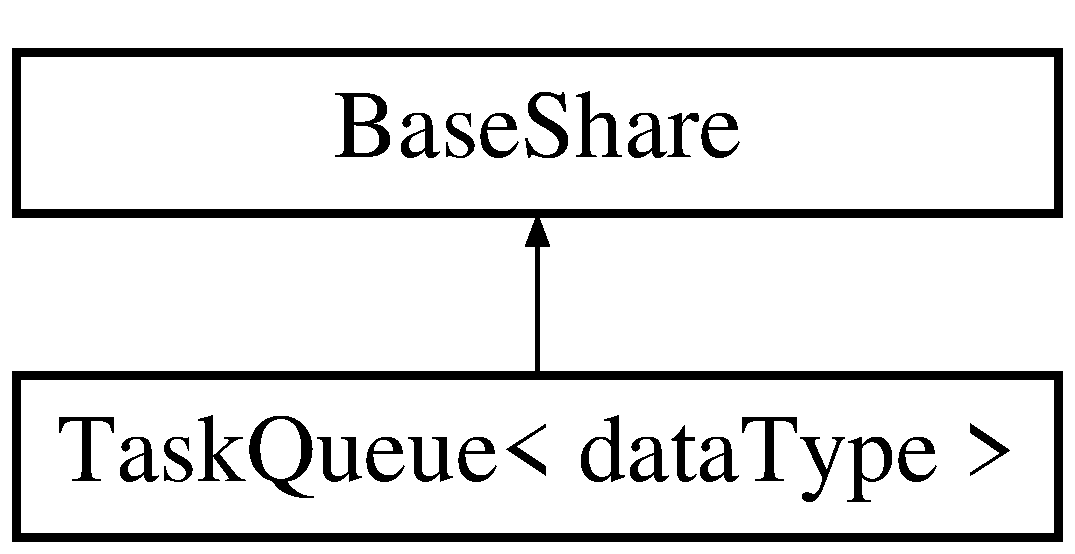
\includegraphics[height=2.000000cm]{class_task_queue}
\end{center}
\end{figure}
\subsection*{Public Member Functions}
\begin{DoxyCompactItemize}
\item 
\mbox{\hyperlink{class_task_queue_a6eb3342ef8f6413673f1d718c1402385}{Task\+Queue}} (Base\+Type\+\_\+t queue\+\_\+size, const char $\ast$p\+\_\+name, \mbox{\hyperlink{classemstream}{emstream}} $\ast$=N\+U\+LL, Tick\+Type\+\_\+t=port\+M\+A\+X\+\_\+\+D\+E\+L\+AY)
\begin{DoxyCompactList}\small\item\em Construct a queue object, allocating memory for the buffer. \end{DoxyCompactList}\item 
\mbox{\hyperlink{group___motor___boolean___type_ga0ecf26b576b9a54eca656b9be7ba6a06}{bool}} \mbox{\hyperlink{class_task_queue_ad1dac62fcf253ab0cf50e47654c5fb29}{put}} (const data\+Type \&item)
\begin{DoxyCompactList}\small\item\em Put an item into the queue behind other items. \end{DoxyCompactList}\item 
\mbox{\hyperlink{group___motor___boolean___type_ga0ecf26b576b9a54eca656b9be7ba6a06}{bool}} \mbox{\hyperlink{class_task_queue_a51ff464dfa1c2be2beae36fdd9e36b44}{I\+S\+R\+\_\+put}} (const data\+Type \&item)
\begin{DoxyCompactList}\small\item\em Put an item into the queue from within an I\+SR. \end{DoxyCompactList}\item 
\mbox{\hyperlink{group___motor___boolean___type_ga0ecf26b576b9a54eca656b9be7ba6a06}{bool}} \mbox{\hyperlink{class_task_queue_a7c2810b4a2137dd88bc72fd1f20d18eb}{butt\+\_\+in}} (const data\+Type \&item)
\begin{DoxyCompactList}\small\item\em Put an item into the front of the queue to be retrieved first. \end{DoxyCompactList}\item 
\mbox{\hyperlink{group___motor___boolean___type_ga0ecf26b576b9a54eca656b9be7ba6a06}{bool}} \mbox{\hyperlink{class_task_queue_aa3d85ebdbee24d455f97b37a018f0230}{I\+S\+R\+\_\+butt\+\_\+in}} (const data\+Type \&item)
\begin{DoxyCompactList}\small\item\em Put an item into the front of the queue from within an I\+SR. \end{DoxyCompactList}\item 
\mbox{\hyperlink{group___motor___boolean___type_ga0ecf26b576b9a54eca656b9be7ba6a06}{bool}} \mbox{\hyperlink{class_task_queue_a29c1d8b98bcb89d77919ad9ce69320a1}{is\+\_\+empty}} (void)
\begin{DoxyCompactList}\small\item\em Return true if the queue is empty. \end{DoxyCompactList}\item 
\mbox{\hyperlink{group___motor___boolean___type_ga0ecf26b576b9a54eca656b9be7ba6a06}{bool}} \mbox{\hyperlink{class_task_queue_a15630b93ea2a6428aff8234213fac24f}{I\+S\+R\+\_\+is\+\_\+empty}} (void)
\begin{DoxyCompactList}\small\item\em Return true if the queue is empty, from within an I\+SR. \end{DoxyCompactList}\item 
data\+Type \mbox{\hyperlink{class_task_queue_a8b696b7e87f4e1bb5cfde83f91dcef75}{get}} (void)
\begin{DoxyCompactList}\small\item\em Return and remove the item at the head of the queue. \end{DoxyCompactList}\item 
data\+Type \mbox{\hyperlink{class_task_queue_a57f0fd2a291dacf66983942b82e2997b}{I\+S\+R\+\_\+get}} (void)
\begin{DoxyCompactList}\small\item\em Return and remove the item at the head of the queue from within an I\+SR. \end{DoxyCompactList}\item 
data\+Type \mbox{\hyperlink{class_task_queue_a696a695c31e089cf2361f8a16c2fefe6}{look\+\_\+at}} (void)
\begin{DoxyCompactList}\small\item\em Return the item at the queue head without removing it. \end{DoxyCompactList}\item 
data\+Type \mbox{\hyperlink{class_task_queue_a5f13cf022edebc95b8c9ca36814a820b}{I\+S\+R\+\_\+look\+\_\+at}} (void)
\begin{DoxyCompactList}\small\item\em Return the item at the front of the queue without deleting it, from within an I\+SR. \end{DoxyCompactList}\item 
\mbox{\hyperlink{group___motor___boolean___type_ga0ecf26b576b9a54eca656b9be7ba6a06}{bool}} \mbox{\hyperlink{class_task_queue_a0c24c84baac830cce4d6f528a0eee23c}{not\+\_\+empty}} (void)
\begin{DoxyCompactList}\small\item\em Return true if the queue has contents which can be read. \end{DoxyCompactList}\item 
\mbox{\hyperlink{group___motor___boolean___type_ga0ecf26b576b9a54eca656b9be7ba6a06}{bool}} \mbox{\hyperlink{class_task_queue_a805c30a60f68150f538577aaaab39e74}{I\+S\+R\+\_\+not\+\_\+empty}} (void)
\begin{DoxyCompactList}\small\item\em Return true if the queue has items in it, from within an I\+SR. \end{DoxyCompactList}\item 
unsigned port\+B\+A\+S\+E\+\_\+\+T\+Y\+PE \mbox{\hyperlink{class_task_queue_af6084d7ce87cefdfb3891dee4b3dfcfe}{num\+\_\+items\+\_\+in}} (void)
\begin{DoxyCompactList}\small\item\em Return the number of items in the queue. \end{DoxyCompactList}\item 
unsigned port\+B\+A\+S\+E\+\_\+\+T\+Y\+PE \mbox{\hyperlink{class_task_queue_af3589846ebd5b842b0b74ffa7e1029af}{I\+S\+R\+\_\+num\+\_\+items\+\_\+in}} (void)
\begin{DoxyCompactList}\small\item\em Return the number of items in the queue, to an I\+SR. \end{DoxyCompactList}\item 
void \mbox{\hyperlink{class_task_queue_ad5ccb9c99ca4f43304d408d915314d71}{print\+\_\+in\+\_\+list}} (\mbox{\hyperlink{classemstream}{emstream}} $\ast$p\+\_\+ser\+\_\+dev)
\begin{DoxyCompactList}\small\item\em Print the queue\textquotesingle{}s status to a serial device. \end{DoxyCompactList}\item 
Queue\+Handle\+\_\+t \mbox{\hyperlink{class_task_queue_a76d88ebf1c89534addd90863cb0a1015}{get\+\_\+handle}} (void)
\begin{DoxyCompactList}\small\item\em Return a handle to the Free\+R\+T\+OS structure which runs this queue. \end{DoxyCompactList}\end{DoxyCompactItemize}
\subsection*{Protected Attributes}
\begin{DoxyCompactItemize}
\item 
\mbox{\Hypertarget{class_task_queue_a9e2438ecd0f75063540296b04f3b511e}\label{class_task_queue_a9e2438ecd0f75063540296b04f3b511e}} 
Queue\+Handle\+\_\+t \mbox{\hyperlink{class_task_queue_a9e2438ecd0f75063540296b04f3b511e}{handle}}
\begin{DoxyCompactList}\small\item\em The handle for the queue we use. \end{DoxyCompactList}\item 
\mbox{\Hypertarget{class_task_queue_ad969b6d7fe091778283bc8cc1b6792bd}\label{class_task_queue_ad969b6d7fe091778283bc8cc1b6792bd}} 
Tick\+Type\+\_\+t \mbox{\hyperlink{class_task_queue_ad969b6d7fe091778283bc8cc1b6792bd}{ticks\+\_\+to\+\_\+wait}}
\begin{DoxyCompactList}\small\item\em R\+T\+OS ticks to wait for empty queue. \end{DoxyCompactList}\item 
\mbox{\Hypertarget{class_task_queue_a8b168989633f215a8f1c8b4a399b8782}\label{class_task_queue_a8b168989633f215a8f1c8b4a399b8782}} 
\mbox{\hyperlink{classemstream}{emstream}} $\ast$ \mbox{\hyperlink{class_task_queue_a8b168989633f215a8f1c8b4a399b8782}{p\+\_\+serial}}
\begin{DoxyCompactList}\small\item\em Serial device for debugging info. \end{DoxyCompactList}\item 
\mbox{\Hypertarget{class_task_queue_af4c4635ceb7cd5f0f331301285b5c211}\label{class_task_queue_af4c4635ceb7cd5f0f331301285b5c211}} 
uint16\+\_\+t \mbox{\hyperlink{class_task_queue_af4c4635ceb7cd5f0f331301285b5c211}{buf\+\_\+size}}
\begin{DoxyCompactList}\small\item\em Size of queue buffer in bytes. \end{DoxyCompactList}\item 
\mbox{\Hypertarget{class_task_queue_a93a34bc4223badccc7ca6afd6b16ec99}\label{class_task_queue_a93a34bc4223badccc7ca6afd6b16ec99}} 
uint16\+\_\+t \mbox{\hyperlink{class_task_queue_a93a34bc4223badccc7ca6afd6b16ec99}{max\+\_\+full}}
\begin{DoxyCompactList}\small\item\em Maximum number of bytes in queue. \end{DoxyCompactList}\end{DoxyCompactItemize}
\subsection*{Additional Inherited Members}


\subsection{Detailed Description}
\subsubsection*{template$<$class data\+Type$>$\newline
class Task\+Queue$<$ data\+Type $>$}

Implements a queue to transmit data from one R\+T\+OS task to another. 

Since multithreaded tasks must not use unprotected shared data items for communication, queues are a primary means of intertask communication. Other means include shared data items (see \mbox{\hyperlink{taskshare_8h}{taskshare.\+h}}) and carrier pigeons. The use of a C++ class template allows the compiler to check that you\textquotesingle{}re putting the right type of data into each queue and getting the right type of data out, thus helping to prevent programming mistakes that can corrupt your data.

As a template class, {\ttfamily Task\+Queue$<$data\+Type$>$} can be used to make queues which hold data of many types. \char`\"{}\+Plain Old Data\char`\"{} types such as {\ttfamily bool} or {\ttfamily uint16\+\_\+t} are supported, of course. But you can also use queues which hold compound data types. For example, if you have {\ttfamily class my\+\_\+data} which holds several measurements together in an object, you can make a queue for {\ttfamily my\+\_\+data} objects with {\ttfamily Task\+Queue$<$my\+\_\+data$>$}. Each item in the queue will then hold several measurements. The size of Free\+R\+T\+OS queues is limited to 255 items in 8-\/bit microcontrollers whose {\ttfamily port\+B\+A\+S\+E\+\_\+\+T\+Y\+PE} is an 8-\/bit number. This is a Free\+R\+T\+OS feature.

Normal writing and reading are done with methods {\ttfamily \mbox{\hyperlink{class_task_queue_ad1dac62fcf253ab0cf50e47654c5fb29}{put()}}} and {\ttfamily \mbox{\hyperlink{class_task_queue_a8b696b7e87f4e1bb5cfde83f91dcef75}{get()}}}. Normal writing means that the sending task must wait until there is empty space in the queue, and then it puts a data item into the \char`\"{}back\char`\"{} of the queue, where \char`\"{}back\char`\"{} means that the item in the back of the queue will be read after all items that were previously put into the queue have been read. Normal reading means that when an item is read from the front of the queue, it will then be removed, making space for more items at the back. This process is often used to synchronize tasks, as the reading task\textquotesingle{}s {\ttfamily \mbox{\hyperlink{class_task_queue_a8b696b7e87f4e1bb5cfde83f91dcef75}{get()}}} method blocks, meaning that the reading task gets stuck waiting for an item to arrive in the queue; it won\textquotesingle{}t do anything useful until new data has been read. Note that this is acceptable behavior in an R\+T\+OS because the R\+T\+OS scheduler will ensure that other tasks get to run even while the reading task is blocking itself waiting for data.

In some cases, one may need to use less normal reading and writing methods. Methods whose name begins with {\ttfamily I\+S\+R\+\_\+} are to be used only within a hardware interrupt service routine. If one needs to put data at the front of the queue instead of the back, use {\ttfamily \mbox{\hyperlink{class_task_queue_a7c2810b4a2137dd88bc72fd1f20d18eb}{butt\+\_\+in()}}} instead of {\ttfamily \mbox{\hyperlink{class_task_queue_ad1dac62fcf253ab0cf50e47654c5fb29}{put()}}}. If one needs to read data from the queue without removing that data, the {\ttfamily \mbox{\hyperlink{class_task_queue_a696a695c31e089cf2361f8a16c2fefe6}{look\+\_\+at()}}} method allows this to be done. If something particularly unusual needs to be done with the queue, one can use the method {\ttfamily \mbox{\hyperlink{class_task_queue_a76d88ebf1c89534addd90863cb0a1015}{get\+\_\+handle()}}} to retrieve the handle used by the C language functions in Free\+R\+T\+OS to access the \mbox{\hyperlink{class_task_queue}{Task\+Queue}} object\textquotesingle{}s underlying data structure directly.\hypertarget{index_Usage}{}\subsection{Usage}\label{index_Usage}
The following bits of code show how to set up and use a queue to transfer data of type {\ttfamily uint16\+\_\+t} from one hypothetical task called {\ttfamily task\+\_\+A} to another called {\ttfamily task\+\_\+B}.

In the file which contains {\ttfamily \mbox{\hyperlink{main_8cpp_a840291bc02cba5474a4cb46a9b9566fe}{main()}}} we create a pointer to a queue and use the {\ttfamily new} operator to create the queue itself. The constructor of the {\ttfamily Task\+Queue$<$uint16\+\_\+t$>$} class is given the number of items in the queue (10) and a pointer to a serial port object named {\ttfamily serial\+\_\+port} that has previously been created\+: 
\begin{DoxyCode}
\mbox{\hyperlink{class_task_queue}{TaskQueue<uint16\_t>}}* p\_my\_queue;
...
main ()
\{
    ...
    p\_my\_queue = \textcolor{keyword}{new} \mbox{\hyperlink{class_task_queue}{TaskQueue<uint16\_t>}} (10, \textcolor{stringliteral}{"Data1"});
\}
\end{DoxyCode}
 In a header file which is read by all the source files in the project we re-\/declare the queue pointer with the keyword {\ttfamily extern} to make it globally accessible in all files that {\ttfamily \#include} this header file\+: 
\begin{DoxyCode}
\textcolor{keyword}{extern} \mbox{\hyperlink{class_task_queue}{TaskQueue<uint16\_t>}}* p\_my\_queue;
\end{DoxyCode}
 In the sending task, data is put into the queue\+: 
\begin{DoxyCode}
uint16\_t a\_data\_item;
...
p\_my\_queue->put (a\_data\_item);
\end{DoxyCode}
 In the receiving task, data is read from the queue. In typical usage, the call to {\ttfamily get\+\_\+out()} will block the receiving task until data is put into the queue by the sending task\+: 
\begin{DoxyCode}
uint16\_t got\_data;
...
got\_data = p\_my\_queue->\mbox{\hyperlink{class_task_queue_a8b696b7e87f4e1bb5cfde83f91dcef75}{get}} ();
\end{DoxyCode}
 

\subsection{Constructor \& Destructor Documentation}
\mbox{\Hypertarget{class_task_queue_a6eb3342ef8f6413673f1d718c1402385}\label{class_task_queue_a6eb3342ef8f6413673f1d718c1402385}} 
\index{Task\+Queue@{Task\+Queue}!Task\+Queue@{Task\+Queue}}
\index{Task\+Queue@{Task\+Queue}!Task\+Queue@{Task\+Queue}}
\subsubsection{\texorpdfstring{Task\+Queue()}{TaskQueue()}}
{\footnotesize\ttfamily template$<$class data\+Type $>$ \\
\mbox{\hyperlink{class_task_queue}{Task\+Queue}}$<$ data\+Type $>$\+::\mbox{\hyperlink{class_task_queue}{Task\+Queue}} (\begin{DoxyParamCaption}\item[{Base\+Type\+\_\+t}]{queue\+\_\+size,  }\item[{const char $\ast$}]{p\+\_\+name,  }\item[{\mbox{\hyperlink{classemstream}{emstream}} $\ast$}]{p\+\_\+ser\+\_\+dev = {\ttfamily NULL},  }\item[{Tick\+Type\+\_\+t}]{wait\+\_\+time = {\ttfamily portMAX\+\_\+DELAY} }\end{DoxyParamCaption})}



Construct a queue object, allocating memory for the buffer. 

This constructor creates the Free\+R\+T\+OS queue which is wrapped by the {\ttfamily \mbox{\hyperlink{class_task_queue}{Task\+Queue}}} class. 
\begin{DoxyParams}{Parameters}
{\em queue\+\_\+size} & The number of characters which can be stored in the queue \\
\hline
{\em p\+\_\+name} & A name to be shown in the list of task shares (default {\ttfamily N\+U\+LL}) \\
\hline
{\em p\+\_\+ser\+\_\+dev} & Pointer to a serial device to be used for debugging printouts Default\+: {\ttfamily N\+U\+LL} \\
\hline
{\em wait\+\_\+time} & How long, in R\+T\+OS ticks, to wait for a full queue to become empty before a character can be sent. Default\+: {\ttfamily port\+M\+A\+X\+\_\+\+D\+E\+L\+AY} which causes the sending task to block until sending occurs. \\
\hline
\end{DoxyParams}


\subsection{Member Function Documentation}
\mbox{\Hypertarget{class_task_queue_a7c2810b4a2137dd88bc72fd1f20d18eb}\label{class_task_queue_a7c2810b4a2137dd88bc72fd1f20d18eb}} 
\index{Task\+Queue@{Task\+Queue}!butt\+\_\+in@{butt\+\_\+in}}
\index{butt\+\_\+in@{butt\+\_\+in}!Task\+Queue@{Task\+Queue}}
\subsubsection{\texorpdfstring{butt\+\_\+in()}{butt\_in()}}
{\footnotesize\ttfamily template$<$class data\+Type$>$ \\
\mbox{\hyperlink{group___motor___boolean___type_ga0ecf26b576b9a54eca656b9be7ba6a06}{bool}} \mbox{\hyperlink{class_task_queue}{Task\+Queue}}$<$ data\+Type $>$\+::butt\+\_\+in (\begin{DoxyParamCaption}\item[{const data\+Type \&}]{item }\end{DoxyParamCaption})\hspace{0.3cm}{\ttfamily [inline]}}



Put an item into the front of the queue to be retrieved first. 

This method puts an item into the front of the queue so that it will be received first as long as nothing else is put in front of it. This is not the normal way to put things into a queue; using {\ttfamily \mbox{\hyperlink{class_task_queue_ad1dac62fcf253ab0cf50e47654c5fb29}{put()}}} to put items into the back of the queue is. If you always use this method, you\textquotesingle{}re really making a stack rather than a queue, you weirdo. This method must {\bfseries not} be used within an interrupt service routine. 
\begin{DoxyParams}{Parameters}
{\em item} & Reference to the item which is going to be (rudely) put into the front of the queue \\
\hline
\end{DoxyParams}
\begin{DoxyReturn}{Returns}
True if the item was successfully queued, false if not 
\end{DoxyReturn}
\mbox{\Hypertarget{class_task_queue_a8b696b7e87f4e1bb5cfde83f91dcef75}\label{class_task_queue_a8b696b7e87f4e1bb5cfde83f91dcef75}} 
\index{Task\+Queue@{Task\+Queue}!get@{get}}
\index{get@{get}!Task\+Queue@{Task\+Queue}}
\subsubsection{\texorpdfstring{get()}{get()}}
{\footnotesize\ttfamily template$<$class data\+Type $>$ \\
data\+Type \mbox{\hyperlink{class_task_queue}{Task\+Queue}}$<$ data\+Type $>$\+::get (\begin{DoxyParamCaption}\item[{void}]{ }\end{DoxyParamCaption})\hspace{0.3cm}{\ttfamily [inline]}}



Return and remove the item at the head of the queue. 

This method returns the item at the head of the queue and removes that item from the queue. If there\textquotesingle{}s nothing in the queue, this method waits, blocking the calling task, for the number of R\+T\+OS ticks specified in the {\ttfamily wait\+\_\+time} parameter to the queue constructor (the default is forever) or until something shows up. \begin{DoxyReturn}{Returns}
The data retrieved from the queue 
\end{DoxyReturn}
\mbox{\Hypertarget{class_task_queue_a76d88ebf1c89534addd90863cb0a1015}\label{class_task_queue_a76d88ebf1c89534addd90863cb0a1015}} 
\index{Task\+Queue@{Task\+Queue}!get\+\_\+handle@{get\+\_\+handle}}
\index{get\+\_\+handle@{get\+\_\+handle}!Task\+Queue@{Task\+Queue}}
\subsubsection{\texorpdfstring{get\+\_\+handle()}{get\_handle()}}
{\footnotesize\ttfamily template$<$class data\+Type$>$ \\
Queue\+Handle\+\_\+t \mbox{\hyperlink{class_task_queue}{Task\+Queue}}$<$ data\+Type $>$\+::get\+\_\+handle (\begin{DoxyParamCaption}\item[{void}]{ }\end{DoxyParamCaption})\hspace{0.3cm}{\ttfamily [inline]}}



Return a handle to the Free\+R\+T\+OS structure which runs this queue. 

If somebody wants to do something which Free\+R\+T\+OS queues can do but this class doesn\textquotesingle{}t support, a handle for the queue wrapped by this class can be used to access the queue directly. This isn\textquotesingle{}t normally done. \begin{DoxyReturn}{Returns}
The handle of the Free\+R\+T\+OS queue which is wrapped within this C++ class 
\end{DoxyReturn}
\mbox{\Hypertarget{class_task_queue_a29c1d8b98bcb89d77919ad9ce69320a1}\label{class_task_queue_a29c1d8b98bcb89d77919ad9ce69320a1}} 
\index{Task\+Queue@{Task\+Queue}!is\+\_\+empty@{is\+\_\+empty}}
\index{is\+\_\+empty@{is\+\_\+empty}!Task\+Queue@{Task\+Queue}}
\subsubsection{\texorpdfstring{is\+\_\+empty()}{is\_empty()}}
{\footnotesize\ttfamily template$<$class data\+Type$>$ \\
\mbox{\hyperlink{group___motor___boolean___type_ga0ecf26b576b9a54eca656b9be7ba6a06}{bool}} \mbox{\hyperlink{class_task_queue}{Task\+Queue}}$<$ data\+Type $>$\+::is\+\_\+empty (\begin{DoxyParamCaption}\item[{void}]{ }\end{DoxyParamCaption})\hspace{0.3cm}{\ttfamily [inline]}}



Return true if the queue is empty. 

This method checks if the queue is empty. It returns {\ttfamily true} if there are no items in the queue and {\ttfamily false} if there are items. \begin{DoxyReturn}{Returns}
{\ttfamily true} if the queue is empty, {\ttfamily false} if it\textquotesingle{}s not empty 
\end{DoxyReturn}
\mbox{\Hypertarget{class_task_queue_aa3d85ebdbee24d455f97b37a018f0230}\label{class_task_queue_aa3d85ebdbee24d455f97b37a018f0230}} 
\index{Task\+Queue@{Task\+Queue}!I\+S\+R\+\_\+butt\+\_\+in@{I\+S\+R\+\_\+butt\+\_\+in}}
\index{I\+S\+R\+\_\+butt\+\_\+in@{I\+S\+R\+\_\+butt\+\_\+in}!Task\+Queue@{Task\+Queue}}
\subsubsection{\texorpdfstring{I\+S\+R\+\_\+butt\+\_\+in()}{ISR\_butt\_in()}}
{\footnotesize\ttfamily template$<$class data\+Type $>$ \\
\mbox{\hyperlink{group___motor___boolean___type_ga0ecf26b576b9a54eca656b9be7ba6a06}{bool}} \mbox{\hyperlink{class_task_queue}{Task\+Queue}}$<$ data\+Type $>$\+::I\+S\+R\+\_\+butt\+\_\+in (\begin{DoxyParamCaption}\item[{const data\+Type \&}]{item }\end{DoxyParamCaption})}



Put an item into the front of the queue from within an I\+SR. 

This method puts an item into the front of the queue from within an I\+SR. It must {\bfseries not} be used within normal, non-\/\+I\+SR code. 
\begin{DoxyParams}{Parameters}
{\em item} & The item which is going to be (rudely) put into the front of the queue \\
\hline
\end{DoxyParams}
\begin{DoxyReturn}{Returns}
True if the item was successfully queued, false if not 
\end{DoxyReturn}
\mbox{\Hypertarget{class_task_queue_a57f0fd2a291dacf66983942b82e2997b}\label{class_task_queue_a57f0fd2a291dacf66983942b82e2997b}} 
\index{Task\+Queue@{Task\+Queue}!I\+S\+R\+\_\+get@{I\+S\+R\+\_\+get}}
\index{I\+S\+R\+\_\+get@{I\+S\+R\+\_\+get}!Task\+Queue@{Task\+Queue}}
\subsubsection{\texorpdfstring{I\+S\+R\+\_\+get()}{ISR\_get()}}
{\footnotesize\ttfamily template$<$class data\+Type $>$ \\
data\+Type \mbox{\hyperlink{class_task_queue}{Task\+Queue}}$<$ data\+Type $>$\+::I\+S\+R\+\_\+get (\begin{DoxyParamCaption}\item[{void}]{ }\end{DoxyParamCaption})\hspace{0.3cm}{\ttfamily [inline]}}



Return and remove the item at the head of the queue from within an I\+SR. 

This method removes and returns the item at the head of the queue from within an interrupt service routine. This method must {\bfseries not} be called from within normal non-\/\+I\+SR code. \begin{DoxyReturn}{Returns}
The data retrieved from the queue 
\end{DoxyReturn}
\mbox{\Hypertarget{class_task_queue_a15630b93ea2a6428aff8234213fac24f}\label{class_task_queue_a15630b93ea2a6428aff8234213fac24f}} 
\index{Task\+Queue@{Task\+Queue}!I\+S\+R\+\_\+is\+\_\+empty@{I\+S\+R\+\_\+is\+\_\+empty}}
\index{I\+S\+R\+\_\+is\+\_\+empty@{I\+S\+R\+\_\+is\+\_\+empty}!Task\+Queue@{Task\+Queue}}
\subsubsection{\texorpdfstring{I\+S\+R\+\_\+is\+\_\+empty()}{ISR\_is\_empty()}}
{\footnotesize\ttfamily template$<$class data\+Type$>$ \\
\mbox{\hyperlink{group___motor___boolean___type_ga0ecf26b576b9a54eca656b9be7ba6a06}{bool}} \mbox{\hyperlink{class_task_queue}{Task\+Queue}}$<$ data\+Type $>$\+::I\+S\+R\+\_\+is\+\_\+empty (\begin{DoxyParamCaption}\item[{void}]{ }\end{DoxyParamCaption})\hspace{0.3cm}{\ttfamily [inline]}}



Return true if the queue is empty, from within an I\+SR. 

This method checks if the queue is empty from within an interrupt service routine. It must not be used in normal non-\/\+I\+SR code. \begin{DoxyReturn}{Returns}
{\ttfamily true} if the queue is empty, {\ttfamily false} if it\textquotesingle{}s not empty 
\end{DoxyReturn}
\mbox{\Hypertarget{class_task_queue_a5f13cf022edebc95b8c9ca36814a820b}\label{class_task_queue_a5f13cf022edebc95b8c9ca36814a820b}} 
\index{Task\+Queue@{Task\+Queue}!I\+S\+R\+\_\+look\+\_\+at@{I\+S\+R\+\_\+look\+\_\+at}}
\index{I\+S\+R\+\_\+look\+\_\+at@{I\+S\+R\+\_\+look\+\_\+at}!Task\+Queue@{Task\+Queue}}
\subsubsection{\texorpdfstring{I\+S\+R\+\_\+look\+\_\+at()}{ISR\_look\_at()}}
{\footnotesize\ttfamily template$<$class data\+Type $>$ \\
data\+Type \mbox{\hyperlink{class_task_queue}{Task\+Queue}}$<$ data\+Type $>$\+::I\+S\+R\+\_\+look\+\_\+at (\begin{DoxyParamCaption}\item[{void}]{ }\end{DoxyParamCaption})\hspace{0.3cm}{\ttfamily [inline]}}



Return the item at the front of the queue without deleting it, from within an I\+SR. 

This method returns the item at the head of the queue without removing that item from the queue. If there\textquotesingle{}s nothing in the queue, this method returns the result of the default constructor for the data item, usually zero in the given data type. This method must {\bfseries not} be called from within an interrupt service routine. \begin{DoxyReturn}{Returns}
The data retrieved from the queue; the data is set to 0 in the correct data type if we couldn\textquotesingle{}t get any data from the queue 
\end{DoxyReturn}
\mbox{\Hypertarget{class_task_queue_a805c30a60f68150f538577aaaab39e74}\label{class_task_queue_a805c30a60f68150f538577aaaab39e74}} 
\index{Task\+Queue@{Task\+Queue}!I\+S\+R\+\_\+not\+\_\+empty@{I\+S\+R\+\_\+not\+\_\+empty}}
\index{I\+S\+R\+\_\+not\+\_\+empty@{I\+S\+R\+\_\+not\+\_\+empty}!Task\+Queue@{Task\+Queue}}
\subsubsection{\texorpdfstring{I\+S\+R\+\_\+not\+\_\+empty()}{ISR\_not\_empty()}}
{\footnotesize\ttfamily template$<$class data\+Type$>$ \\
\mbox{\hyperlink{group___motor___boolean___type_ga0ecf26b576b9a54eca656b9be7ba6a06}{bool}} \mbox{\hyperlink{class_task_queue}{Task\+Queue}}$<$ data\+Type $>$\+::I\+S\+R\+\_\+not\+\_\+empty (\begin{DoxyParamCaption}\item[{void}]{ }\end{DoxyParamCaption})\hspace{0.3cm}{\ttfamily [inline]}}



Return true if the queue has items in it, from within an I\+SR. 

This method allows one to check if the queue has any contents from within an interrupt service routine. It must {\bfseries not} be used from within normal, non-\/\+I\+SR code. \begin{DoxyReturn}{Returns}
{\ttfamily true} if there\textquotesingle{}s something in the queue, {\ttfamily false} if not 
\end{DoxyReturn}
\mbox{\Hypertarget{class_task_queue_af3589846ebd5b842b0b74ffa7e1029af}\label{class_task_queue_af3589846ebd5b842b0b74ffa7e1029af}} 
\index{Task\+Queue@{Task\+Queue}!I\+S\+R\+\_\+num\+\_\+items\+\_\+in@{I\+S\+R\+\_\+num\+\_\+items\+\_\+in}}
\index{I\+S\+R\+\_\+num\+\_\+items\+\_\+in@{I\+S\+R\+\_\+num\+\_\+items\+\_\+in}!Task\+Queue@{Task\+Queue}}
\subsubsection{\texorpdfstring{I\+S\+R\+\_\+num\+\_\+items\+\_\+in()}{ISR\_num\_items\_in()}}
{\footnotesize\ttfamily template$<$class data\+Type$>$ \\
unsigned port\+B\+A\+S\+E\+\_\+\+T\+Y\+PE \mbox{\hyperlink{class_task_queue}{Task\+Queue}}$<$ data\+Type $>$\+::I\+S\+R\+\_\+num\+\_\+items\+\_\+in (\begin{DoxyParamCaption}\item[{void}]{ }\end{DoxyParamCaption})\hspace{0.3cm}{\ttfamily [inline]}}



Return the number of items in the queue, to an I\+SR. 

This method returns the number of items waiting in the queue; it must be called only from within an interrupt service routine. \begin{DoxyReturn}{Returns}
The number of items in the queue 
\end{DoxyReturn}
\mbox{\Hypertarget{class_task_queue_a51ff464dfa1c2be2beae36fdd9e36b44}\label{class_task_queue_a51ff464dfa1c2be2beae36fdd9e36b44}} 
\index{Task\+Queue@{Task\+Queue}!I\+S\+R\+\_\+put@{I\+S\+R\+\_\+put}}
\index{I\+S\+R\+\_\+put@{I\+S\+R\+\_\+put}!Task\+Queue@{Task\+Queue}}
\subsubsection{\texorpdfstring{I\+S\+R\+\_\+put()}{ISR\_put()}}
{\footnotesize\ttfamily template$<$class data\+Type $>$ \\
\mbox{\hyperlink{group___motor___boolean___type_ga0ecf26b576b9a54eca656b9be7ba6a06}{bool}} \mbox{\hyperlink{class_task_queue}{Task\+Queue}}$<$ data\+Type $>$\+::I\+S\+R\+\_\+put (\begin{DoxyParamCaption}\item[{const data\+Type \&}]{item }\end{DoxyParamCaption})\hspace{0.3cm}{\ttfamily [inline]}}



Put an item into the queue from within an I\+SR. 

This method puts an item of data into the back of the queue from within an interrupt service routine. It must {\bfseries not} be used within non-\/\+I\+SR code. 
\begin{DoxyParams}{Parameters}
{\em item} & Reference to the item which is going to be put into the queue \\
\hline
\end{DoxyParams}
\begin{DoxyReturn}{Returns}
True if the item was successfully queued, false if not 
\end{DoxyReturn}
\mbox{\Hypertarget{class_task_queue_a696a695c31e089cf2361f8a16c2fefe6}\label{class_task_queue_a696a695c31e089cf2361f8a16c2fefe6}} 
\index{Task\+Queue@{Task\+Queue}!look\+\_\+at@{look\+\_\+at}}
\index{look\+\_\+at@{look\+\_\+at}!Task\+Queue@{Task\+Queue}}
\subsubsection{\texorpdfstring{look\+\_\+at()}{look\_at()}}
{\footnotesize\ttfamily template$<$class data\+Type $>$ \\
data\+Type \mbox{\hyperlink{class_task_queue}{Task\+Queue}}$<$ data\+Type $>$\+::look\+\_\+at (\begin{DoxyParamCaption}\item[{void}]{ }\end{DoxyParamCaption})\hspace{0.3cm}{\ttfamily [inline]}}



Return the item at the queue head without removing it. 

This method returns the item at the head of the queue without removing that item from the queue. If there\textquotesingle{}s nothing in the queue, this method waits, blocking the calling task, for for the number of R\+T\+OS ticks specified in the {\ttfamily wait\+\_\+time} parameter to the queue constructor (the default is forever) or until something shows up. This method must {\bfseries not} be called from within an interrupt service routine. \begin{DoxyReturn}{Returns}
The data retrieved from the queue; the data is set to 0 in the correct data type if we couldn\textquotesingle{}t get any data from the queue and the attempt timed out 
\end{DoxyReturn}
\mbox{\Hypertarget{class_task_queue_a0c24c84baac830cce4d6f528a0eee23c}\label{class_task_queue_a0c24c84baac830cce4d6f528a0eee23c}} 
\index{Task\+Queue@{Task\+Queue}!not\+\_\+empty@{not\+\_\+empty}}
\index{not\+\_\+empty@{not\+\_\+empty}!Task\+Queue@{Task\+Queue}}
\subsubsection{\texorpdfstring{not\+\_\+empty()}{not\_empty()}}
{\footnotesize\ttfamily template$<$class data\+Type$>$ \\
\mbox{\hyperlink{group___motor___boolean___type_ga0ecf26b576b9a54eca656b9be7ba6a06}{bool}} \mbox{\hyperlink{class_task_queue}{Task\+Queue}}$<$ data\+Type $>$\+::not\+\_\+empty (\begin{DoxyParamCaption}\item[{void}]{ }\end{DoxyParamCaption})\hspace{0.3cm}{\ttfamily [inline]}}



Return true if the queue has contents which can be read. 

This method allows one to check if the queue has any contents. It must {\bfseries not} be called from within an interrupt service routine. \begin{DoxyReturn}{Returns}
{\ttfamily true} if there\textquotesingle{}s something in the queue, {\ttfamily false} if not 
\end{DoxyReturn}
\mbox{\Hypertarget{class_task_queue_af6084d7ce87cefdfb3891dee4b3dfcfe}\label{class_task_queue_af6084d7ce87cefdfb3891dee4b3dfcfe}} 
\index{Task\+Queue@{Task\+Queue}!num\+\_\+items\+\_\+in@{num\+\_\+items\+\_\+in}}
\index{num\+\_\+items\+\_\+in@{num\+\_\+items\+\_\+in}!Task\+Queue@{Task\+Queue}}
\subsubsection{\texorpdfstring{num\+\_\+items\+\_\+in()}{num\_items\_in()}}
{\footnotesize\ttfamily template$<$class data\+Type$>$ \\
unsigned port\+B\+A\+S\+E\+\_\+\+T\+Y\+PE \mbox{\hyperlink{class_task_queue}{Task\+Queue}}$<$ data\+Type $>$\+::num\+\_\+items\+\_\+in (\begin{DoxyParamCaption}\item[{void}]{ }\end{DoxyParamCaption})\hspace{0.3cm}{\ttfamily [inline]}}



Return the number of items in the queue. 

This method returns the number of items waiting in the queue. It must {\bfseries not} be called from within an interrupt service routine; the method {\ttfamily \mbox{\hyperlink{class_task_queue_af3589846ebd5b842b0b74ffa7e1029af}{I\+S\+R\+\_\+num\+\_\+items\+\_\+in()}}} can be called from within an I\+SR. \begin{DoxyReturn}{Returns}
The number of items in the queue 
\end{DoxyReturn}
\mbox{\Hypertarget{class_task_queue_ad5ccb9c99ca4f43304d408d915314d71}\label{class_task_queue_ad5ccb9c99ca4f43304d408d915314d71}} 
\index{Task\+Queue@{Task\+Queue}!print\+\_\+in\+\_\+list@{print\+\_\+in\+\_\+list}}
\index{print\+\_\+in\+\_\+list@{print\+\_\+in\+\_\+list}!Task\+Queue@{Task\+Queue}}
\subsubsection{\texorpdfstring{print\+\_\+in\+\_\+list()}{print\_in\_list()}}
{\footnotesize\ttfamily template$<$class data\+Type $>$ \\
void \mbox{\hyperlink{class_task_queue}{Task\+Queue}}$<$ data\+Type $>$\+::print\+\_\+in\+\_\+list (\begin{DoxyParamCaption}\item[{\mbox{\hyperlink{classemstream}{emstream}} $\ast$}]{p\+\_\+ser\+\_\+dev }\end{DoxyParamCaption})\hspace{0.3cm}{\ttfamily [virtual]}}



Print the queue\textquotesingle{}s status to a serial device. 

This method makes a printout of the queue\textquotesingle{}s status on the given serial device, then calls this same method for the next item of thread-\/safe data in the linked list of items. 
\begin{DoxyParams}{Parameters}
{\em p\+\_\+ser\+\_\+dev} & Pointer to the serial device on which to print \\
\hline
\end{DoxyParams}


Implements \mbox{\hyperlink{class_base_share_a81ef685c8c1897ee316e853103e9941a}{Base\+Share}}.

\mbox{\Hypertarget{class_task_queue_ad1dac62fcf253ab0cf50e47654c5fb29}\label{class_task_queue_ad1dac62fcf253ab0cf50e47654c5fb29}} 
\index{Task\+Queue@{Task\+Queue}!put@{put}}
\index{put@{put}!Task\+Queue@{Task\+Queue}}
\subsubsection{\texorpdfstring{put()}{put()}}
{\footnotesize\ttfamily template$<$class data\+Type $>$ \\
\mbox{\hyperlink{group___motor___boolean___type_ga0ecf26b576b9a54eca656b9be7ba6a06}{bool}} \mbox{\hyperlink{class_task_queue}{Task\+Queue}}$<$ data\+Type $>$\+::put (\begin{DoxyParamCaption}\item[{const data\+Type \&}]{item }\end{DoxyParamCaption})}



Put an item into the queue behind other items. 

This method puts an item of data into the back of the queue, which is the normal way to put something into a queue. If you want to be rude and put an item into the front of the queue so it will be retreived first, use {\ttfamily \mbox{\hyperlink{class_task_queue_a7c2810b4a2137dd88bc72fd1f20d18eb}{butt\+\_\+in()}}} instead. {\bfseries This method must not be used within an I\+SR.} 
\begin{DoxyParams}{Parameters}
{\em item} & Reference to the item which is going to be put into the queue \\
\hline
\end{DoxyParams}
\begin{DoxyReturn}{Returns}
True if the item was successfully queued, false if not 
\end{DoxyReturn}


The documentation for this class was generated from the following file\+:\begin{DoxyCompactItemize}
\item 
Doxygen\+Files/\mbox{\hyperlink{taskqueue_8h}{taskqueue.\+h}}\end{DoxyCompactItemize}

\hypertarget{class_task_share}{}\section{Task\+Share$<$ Data\+Type $>$ Class Template Reference}
\label{class_task_share}\index{Task\+Share$<$ Data\+Type $>$@{Task\+Share$<$ Data\+Type $>$}}


Class for data to be shared in a thread-\/safe manner between tasks.  




{\ttfamily \#include $<$taskshare.\+h$>$}

Inheritance diagram for Task\+Share$<$ Data\+Type $>$\+:\begin{figure}[H]
\begin{center}
\leavevmode
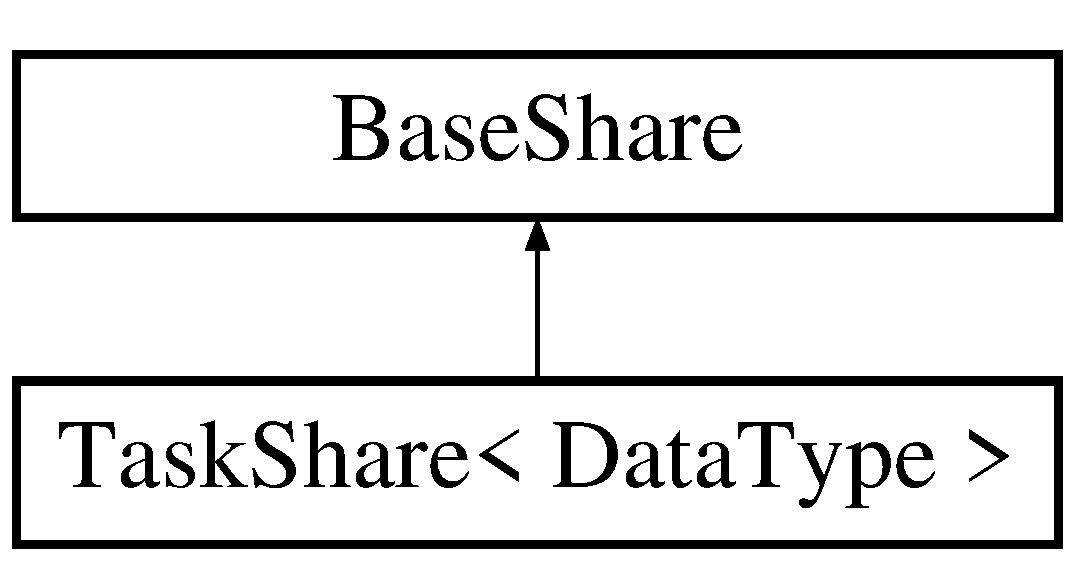
\includegraphics[height=2.000000cm]{class_task_share}
\end{center}
\end{figure}
\subsection*{Public Member Functions}
\begin{DoxyCompactItemize}
\item 
\mbox{\hyperlink{class_task_share_a9e49e43c6da3859b9690a62ad64d7f40}{Task\+Share}} (const char $\ast$p\+\_\+name)
\begin{DoxyCompactList}\small\item\em Construct a shared data item. \end{DoxyCompactList}\item 
void \mbox{\hyperlink{class_task_share_ae1cf7a4f95975446adcfa947d9dabf82}{put}} (Data\+Type)
\begin{DoxyCompactList}\small\item\em Put data into the shared data item. \end{DoxyCompactList}\item 
void \mbox{\hyperlink{class_task_share_a78de768fa4760c6e8f74c7795ff164c7}{I\+S\+R\+\_\+put}} (Data\+Type)
\begin{DoxyCompactList}\small\item\em Put data into the shared data item from within an I\+SR. \end{DoxyCompactList}\item 
Data\+Type \mbox{\hyperlink{class_task_share_a0cf8afd4f4d90c1e91ff2af9a004ecec}{get}} (void)
\begin{DoxyCompactList}\small\item\em Read data from the shared data item. \end{DoxyCompactList}\item 
Data\+Type \mbox{\hyperlink{class_task_share_a5a4bac78053046c248896441a5b3a839}{I\+S\+R\+\_\+get}} (void)
\begin{DoxyCompactList}\small\item\em Read data from the shared data item, from within an I\+SR. \end{DoxyCompactList}\item 
void \mbox{\hyperlink{class_task_share_a08835a91ed7ccd847cefe6ff72fe22e6}{print\+\_\+in\+\_\+list}} (\mbox{\hyperlink{classemstream}{emstream}} $\ast$p\+\_\+ser\+\_\+dev)
\begin{DoxyCompactList}\small\item\em Read data from the shared data item, from within an I\+SR. \end{DoxyCompactList}\item 
Data\+Type \& \mbox{\hyperlink{class_task_share_a8c3b841652c2cde1bfb279aa5bfcc61f}{operator++}} (void)
\begin{DoxyCompactList}\small\item\em The prefix increment causes the shared data to increase by one. \end{DoxyCompactList}\item 
\mbox{\Hypertarget{class_task_share_aaea5630111a55f864b7110456983e0fd}\label{class_task_share_aaea5630111a55f864b7110456983e0fd}} 
Data\+Type \mbox{\hyperlink{class_task_share_aaea5630111a55f864b7110456983e0fd}{operator++}} (int)
\begin{DoxyCompactList}\small\item\em The postfix increment causes the shared data to increase by one. \end{DoxyCompactList}\item 
Data\+Type \& \mbox{\hyperlink{class_task_share_a79024a7661f8f48c5d2303a3fe121a32}{operator-\/-\/}} (void)
\begin{DoxyCompactList}\small\item\em The prefix decrement causes the shared data to decrease by one. \end{DoxyCompactList}\item 
\mbox{\Hypertarget{class_task_share_a55276cb23f2ac2403ad36acf8f3625e3}\label{class_task_share_a55276cb23f2ac2403ad36acf8f3625e3}} 
Data\+Type \mbox{\hyperlink{class_task_share_a55276cb23f2ac2403ad36acf8f3625e3}{operator-\/-\/}} (int)
\begin{DoxyCompactList}\small\item\em The postfix decrement causes the shared data to decrease by one. \end{DoxyCompactList}\end{DoxyCompactItemize}
\subsection*{Protected Attributes}
\begin{DoxyCompactItemize}
\item 
\mbox{\Hypertarget{class_task_share_aa6a83a01a277f67bc5c1a3527b7c3425}\label{class_task_share_aa6a83a01a277f67bc5c1a3527b7c3425}} 
Data\+Type \mbox{\hyperlink{class_task_share_aa6a83a01a277f67bc5c1a3527b7c3425}{the\+\_\+data}}
\begin{DoxyCompactList}\small\item\em Holds the data to be shared. \end{DoxyCompactList}\end{DoxyCompactItemize}
\subsection*{Additional Inherited Members}


\subsection{Detailed Description}
\subsubsection*{template$<$class Data\+Type$>$\newline
class Task\+Share$<$ Data\+Type $>$}

Class for data to be shared in a thread-\/safe manner between tasks. 

This class implements an item of data which can be shared between tasks without risk of data corruption associated with global variables. Unlike queues, shares do not use a buffer for many data items; there is only a one-\/item buffer in which the most recent value of the data is kept. Shares therefore do not provide the task synchronization or incur the overhead associated with queues.

The data is protected by using critical code sections (see the Free\+R\+T\+OS documentation of {\ttfamily port\+E\+N\+T\+E\+R\+\_\+\+C\+R\+I\+T\+I\+C\+A\+L()} ) so that tasks can\textquotesingle{}t interrupt each other when reading or writing the data is taking place. This prevents data corruption due to thread switching. The C++ template mechanism is used to ensure that only data of the correct type is put into or taken from a shared data item. A {\ttfamily Task\+Share$<$\+Data\+Type$>$} object keeps its own separate copy of the data. This uses some memory, but it is necessary to reliably prevent data corruption; it prevents possible side effects from causing the sender\textquotesingle{}s copy of the data from being inadvertently changed.\hypertarget{index_Usage}{}\subsection{Usage}\label{index_Usage}
The following bits of code show how to set up and use a share to transfer data of type {\ttfamily uint16\+\_\+t} from one hypothetical task called {\ttfamily task\+\_\+A} to another called {\ttfamily task\+\_\+B}.

In the file which contains {\ttfamily \mbox{\hyperlink{main_8cpp_a840291bc02cba5474a4cb46a9b9566fe}{main()}}} we create a pointer to a share and use the {\ttfamily new} operator to create the share itself. The constructor of the {\ttfamily Task\+Share$<$uint16\+\_\+t$>$} class is given the name of the share; the name will be shown on system diagnostic printouts\+: 
\begin{DoxyCode}
\mbox{\hyperlink{class_task_share}{TaskShare<uint16\_t>}}* p\_my\_share;
...
main ()
\{
    ...
    p\_my\_share = \textcolor{keyword}{new} \mbox{\hyperlink{class_task_share}{TaskShare<uint16\_t>}} (\textcolor{stringliteral}{"Data\_3"});
\}
\end{DoxyCode}
 In a header file which is read by all the source files in the project we re-\/declare the share pointer with the keyword {\ttfamily extern} to make it globally accessible in all files that {\ttfamily \#include} this header file\+: 
\begin{DoxyCode}
\textcolor{keyword}{extern} \mbox{\hyperlink{class_task_share}{TaskShare<uint16\_t>}}* p\_my\_share;
\end{DoxyCode}
 In the sending task, data is put into the share\+: 
\begin{DoxyCode}
uint16\_t a\_data\_item;
...
p\_my\_share->put (a\_data\_item);
\end{DoxyCode}
 In the receiving task, data is read from the share\+: 
\begin{DoxyCode}
uint16\_t got\_data;
...
got\_data = p\_my\_share->\mbox{\hyperlink{class_task_share_a0cf8afd4f4d90c1e91ff2af9a004ecec}{get}} ();
\end{DoxyCode}


{\bfseries Note\+:} In the past, M\+E405 students have often used task shares to save data persistently within a task. This is {\bfseries not} necessary. Just use variables declared {\ttfamily static} if the data is only needed within one method. If data needs to be shared between member functions of the same task, make such data member data of the task class rather than local data within one method. This data will persist as long as the owning task object exists, which is generally until the power is turned off. 

\subsection{Constructor \& Destructor Documentation}
\mbox{\Hypertarget{class_task_share_a9e49e43c6da3859b9690a62ad64d7f40}\label{class_task_share_a9e49e43c6da3859b9690a62ad64d7f40}} 
\index{Task\+Share@{Task\+Share}!Task\+Share@{Task\+Share}}
\index{Task\+Share@{Task\+Share}!Task\+Share@{Task\+Share}}
\subsubsection{\texorpdfstring{Task\+Share()}{TaskShare()}}
{\footnotesize\ttfamily template$<$class Data\+Type$>$ \\
\mbox{\hyperlink{class_task_share}{Task\+Share}}$<$ Data\+Type $>$\+::\mbox{\hyperlink{class_task_share}{Task\+Share}} (\begin{DoxyParamCaption}\item[{const char $\ast$}]{p\+\_\+name }\end{DoxyParamCaption})\hspace{0.3cm}{\ttfamily [inline]}}



Construct a shared data item. 

This default constructor for a shared data item doesn\textquotesingle{}t do much besides allocate memory because there isn\textquotesingle{}t any particular setup required. Note that the data is {\bfseries not} initialized. 
\begin{DoxyParams}{Parameters}
{\em p\+\_\+name} & A name to be shown in the list of task shares (default {\ttfamily N\+U\+LL}) \\
\hline
\end{DoxyParams}


\subsection{Member Function Documentation}
\mbox{\Hypertarget{class_task_share_a0cf8afd4f4d90c1e91ff2af9a004ecec}\label{class_task_share_a0cf8afd4f4d90c1e91ff2af9a004ecec}} 
\index{Task\+Share@{Task\+Share}!get@{get}}
\index{get@{get}!Task\+Share@{Task\+Share}}
\subsubsection{\texorpdfstring{get()}{get()}}
{\footnotesize\ttfamily template$<$class Data\+Type $>$ \\
Data\+Type \mbox{\hyperlink{class_task_share}{Task\+Share}}$<$ Data\+Type $>$\+::get (\begin{DoxyParamCaption}\item[{void}]{ }\end{DoxyParamCaption})}



Read data from the shared data item. 

This method is used to read data from the shared data item with critical section protection to ensure that the data cannot be corrupted by a task switch. \begin{DoxyReturn}{Returns}
The current value of the shared data item 
\end{DoxyReturn}
\mbox{\Hypertarget{class_task_share_a5a4bac78053046c248896441a5b3a839}\label{class_task_share_a5a4bac78053046c248896441a5b3a839}} 
\index{Task\+Share@{Task\+Share}!I\+S\+R\+\_\+get@{I\+S\+R\+\_\+get}}
\index{I\+S\+R\+\_\+get@{I\+S\+R\+\_\+get}!Task\+Share@{Task\+Share}}
\subsubsection{\texorpdfstring{I\+S\+R\+\_\+get()}{ISR\_get()}}
{\footnotesize\ttfamily template$<$class Data\+Type $>$ \\
Data\+Type \mbox{\hyperlink{class_task_share}{Task\+Share}}$<$ Data\+Type $>$\+::I\+S\+R\+\_\+get (\begin{DoxyParamCaption}\item[{void}]{ }\end{DoxyParamCaption})}



Read data from the shared data item, from within an I\+SR. 

This method is used to enable code within an I\+SR to read data from the shared data item. It must only be called from within an interrupt service routine, not a normal task. This is because critical section protection isn\textquotesingle{}t used here, which is OK, assuming that an interrupt can\textquotesingle{}t be interrupted by another interrupt, which is the case on most small microcontrollers. \begin{DoxyReturn}{Returns}
The current value of the shared data item 
\end{DoxyReturn}
\mbox{\Hypertarget{class_task_share_a78de768fa4760c6e8f74c7795ff164c7}\label{class_task_share_a78de768fa4760c6e8f74c7795ff164c7}} 
\index{Task\+Share@{Task\+Share}!I\+S\+R\+\_\+put@{I\+S\+R\+\_\+put}}
\index{I\+S\+R\+\_\+put@{I\+S\+R\+\_\+put}!Task\+Share@{Task\+Share}}
\subsubsection{\texorpdfstring{I\+S\+R\+\_\+put()}{ISR\_put()}}
{\footnotesize\ttfamily template$<$class Data\+Type $>$ \\
void \mbox{\hyperlink{class_task_share}{Task\+Share}}$<$ Data\+Type $>$\+::I\+S\+R\+\_\+put (\begin{DoxyParamCaption}\item[{Data\+Type}]{new\+\_\+data }\end{DoxyParamCaption})}



Put data into the shared data item from within an I\+SR. 

This method writes data from an I\+SR into the shared data item. It must only be called from within a hardware interrupt, not a normal task. This is because critical section protection isn\textquotesingle{}t used here, which is OK, assuming that an interrupt can\textquotesingle{}t be interrupted by another interrupt, which is the case on most small microcontrollers. 
\begin{DoxyParams}{Parameters}
{\em new\+\_\+data} & The data which is to be written into the shared data item \\
\hline
\end{DoxyParams}
\mbox{\Hypertarget{class_task_share_a8c3b841652c2cde1bfb279aa5bfcc61f}\label{class_task_share_a8c3b841652c2cde1bfb279aa5bfcc61f}} 
\index{Task\+Share@{Task\+Share}!operator++@{operator++}}
\index{operator++@{operator++}!Task\+Share@{Task\+Share}}
\subsubsection{\texorpdfstring{operator++()}{operator++()}}
{\footnotesize\ttfamily template$<$class Data\+Type$>$ \\
Data\+Type\& \mbox{\hyperlink{class_task_share}{Task\+Share}}$<$ Data\+Type $>$\+::operator++ (\begin{DoxyParamCaption}\item[{void}]{ }\end{DoxyParamCaption})\hspace{0.3cm}{\ttfamily [inline]}}



The prefix increment causes the shared data to increase by one. 

This operator just increases by one the variable held by the shared data item. B\+UG\+: It should return a reference to this shared data item, but for some reason the compiler insists it must return a reference to the data. Why is unknown. \mbox{\Hypertarget{class_task_share_a79024a7661f8f48c5d2303a3fe121a32}\label{class_task_share_a79024a7661f8f48c5d2303a3fe121a32}} 
\index{Task\+Share@{Task\+Share}!operator-\/-\/@{operator-\/-\/}}
\index{operator-\/-\/@{operator-\/-\/}!Task\+Share@{Task\+Share}}
\subsubsection{\texorpdfstring{operator-\/-\/()}{operator--()}}
{\footnotesize\ttfamily template$<$class Data\+Type$>$ \\
Data\+Type\& \mbox{\hyperlink{class_task_share}{Task\+Share}}$<$ Data\+Type $>$\+::operator-\/-\/ (\begin{DoxyParamCaption}\item[{void}]{ }\end{DoxyParamCaption})\hspace{0.3cm}{\ttfamily [inline]}}



The prefix decrement causes the shared data to decrease by one. 

This operator just decreases by one the variable held by the shared data item. B\+UG\+: It should return a reference to this shared data item, but for some reason the compiler insists it must return a reference to the data. Why is unknown. \mbox{\Hypertarget{class_task_share_a08835a91ed7ccd847cefe6ff72fe22e6}\label{class_task_share_a08835a91ed7ccd847cefe6ff72fe22e6}} 
\index{Task\+Share@{Task\+Share}!print\+\_\+in\+\_\+list@{print\+\_\+in\+\_\+list}}
\index{print\+\_\+in\+\_\+list@{print\+\_\+in\+\_\+list}!Task\+Share@{Task\+Share}}
\subsubsection{\texorpdfstring{print\+\_\+in\+\_\+list()}{print\_in\_list()}}
{\footnotesize\ttfamily template$<$class Data\+Type $>$ \\
void \mbox{\hyperlink{class_task_share}{Task\+Share}}$<$ Data\+Type $>$\+::print\+\_\+in\+\_\+list (\begin{DoxyParamCaption}\item[{\mbox{\hyperlink{classemstream}{emstream}} $\ast$}]{p\+\_\+ser\+\_\+dev }\end{DoxyParamCaption})\hspace{0.3cm}{\ttfamily [virtual]}}



Read data from the shared data item, from within an I\+SR. 

This method is used to enable code within an I\+SR to read data from the shared data item. It must only be called from within an interrupt service routine, not a normal task. This is because critical section protection isn\textquotesingle{}t used here, which is OK, assuming that an interrupt can\textquotesingle{}t be interrupted by another interrupt, which is the case on most small microcontrollers. 
\begin{DoxyParams}{Parameters}
{\em p\+\_\+ser\+\_\+dev} & Pointer to a serial device on which to print the status \\
\hline
\end{DoxyParams}


Implements \mbox{\hyperlink{class_base_share_a81ef685c8c1897ee316e853103e9941a}{Base\+Share}}.

\mbox{\Hypertarget{class_task_share_ae1cf7a4f95975446adcfa947d9dabf82}\label{class_task_share_ae1cf7a4f95975446adcfa947d9dabf82}} 
\index{Task\+Share@{Task\+Share}!put@{put}}
\index{put@{put}!Task\+Share@{Task\+Share}}
\subsubsection{\texorpdfstring{put()}{put()}}
{\footnotesize\ttfamily template$<$class Data\+Type $>$ \\
void \mbox{\hyperlink{class_task_share}{Task\+Share}}$<$ Data\+Type $>$\+::put (\begin{DoxyParamCaption}\item[{Data\+Type}]{new\+\_\+data }\end{DoxyParamCaption})\hspace{0.3cm}{\ttfamily [inline]}}



Put data into the shared data item. 

This method is used to write data into the shared data item. It\textquotesingle{}s declared {\ttfamily inline} so that instead of a regular function call at the assembly language level, {\ttfamily an\+\_\+object.\+put (x);} will result in the code within this function being inserted directly into the calling function. This is faster than doing a regular function call, which involves pushing the program counter on the stack, pushing parameters, jumping, making space for local variables, jumping back and popping the program counter, yawn, zzz... 
\begin{DoxyParams}{Parameters}
{\em new\+\_\+data} & The data which is to be written \\
\hline
\end{DoxyParams}


The documentation for this class was generated from the following file\+:\begin{DoxyCompactItemize}
\item 
Doxygen\+Files/\mbox{\hyperlink{taskshare_8h}{taskshare.\+h}}\end{DoxyCompactItemize}

\hypertarget{class_text_queue}{}\section{Text\+Queue Class Reference}
\label{class_text_queue}\index{Text\+Queue@{Text\+Queue}}


Converts data to characters with {\ttfamily $<$$<$} and puts them into a Free\+R\+T\+OS queue.  




{\ttfamily \#include $<$textqueue.\+h$>$}

Inheritance diagram for Text\+Queue\+:\begin{figure}[H]
\begin{center}
\leavevmode
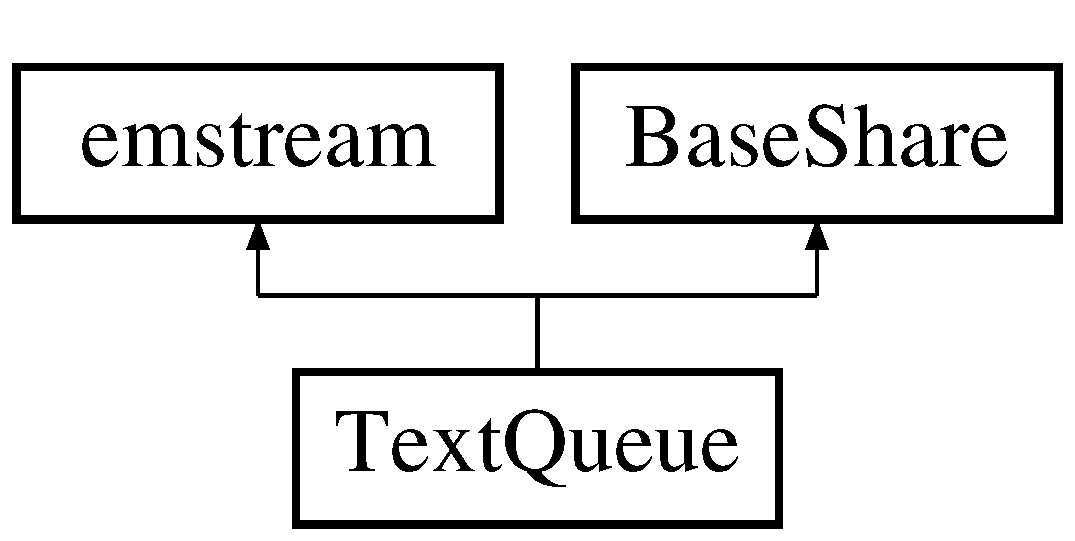
\includegraphics[height=2.000000cm]{class_text_queue}
\end{center}
\end{figure}
\subsection*{Public Member Functions}
\begin{DoxyCompactItemize}
\item 
\mbox{\hyperlink{class_text_queue_a2823917efdf4439cc4f70456b8ddf4bd}{Text\+Queue}} (uint16\+\_\+t size, const char $\ast$p\+\_\+name, \mbox{\hyperlink{classemstream}{emstream}} $\ast$=N\+U\+LL, Tick\+Type\+\_\+t=port\+M\+A\+X\+\_\+\+D\+E\+L\+AY)
\begin{DoxyCompactList}\small\item\em Constructor for a queue which transfers text characters. \end{DoxyCompactList}\item 
void \mbox{\hyperlink{class_text_queue_a917e1c134d4ef6591f832e2706a67cac}{putchar}} (char)
\begin{DoxyCompactList}\small\item\em Write one character to the text queue. \end{DoxyCompactList}\item 
\mbox{\hyperlink{group___motor___boolean___type_ga0ecf26b576b9a54eca656b9be7ba6a06}{bool}} \mbox{\hyperlink{class_text_queue_a4b520515f1110e8d592a3b5a5abc615b}{check\+\_\+for\+\_\+char}} (void)
\begin{DoxyCompactList}\small\item\em Check if a character is ready to be read from the queue. \end{DoxyCompactList}\item 
char \mbox{\hyperlink{class_text_queue_ab682ee4d2cbad87e9496ca424fa03b0a}{getchar}} (void)
\begin{DoxyCompactList}\small\item\em Read one character from the queue. \end{DoxyCompactList}\item 
char \mbox{\hyperlink{class_text_queue_a92ed0a74b86ce1ea2dd426c92f3230c6}{peek}} (void)
\begin{DoxyCompactList}\small\item\em Copy one character from the queue but leave the original there. \end{DoxyCompactList}\item 
\mbox{\hyperlink{class_text_queue_a0fd3c395a00b5da3bb866137466d878a}{operator bool}} () const
\item 
Queue\+Handle\+\_\+t \mbox{\hyperlink{class_text_queue_a0f83656a176a1a4d71ef825b8a423ab7}{get\+\_\+handle}} (void)
\item 
void \mbox{\hyperlink{class_text_queue_aeef41a1bc3486d98fb31cba9ce539d0d}{print\+\_\+in\+\_\+list}} (\mbox{\hyperlink{classemstream}{emstream}} $\ast$p\+\_\+ser\+\_\+dev)
\begin{DoxyCompactList}\small\item\em Print the status of the queue. \end{DoxyCompactList}\end{DoxyCompactItemize}
\subsection*{Protected Attributes}
\begin{DoxyCompactItemize}
\item 
\mbox{\Hypertarget{class_text_queue_a7697f86be6c148f866c97f9ab09fec6f}\label{class_text_queue_a7697f86be6c148f866c97f9ab09fec6f}} 
Queue\+Handle\+\_\+t \mbox{\hyperlink{class_text_queue_a7697f86be6c148f866c97f9ab09fec6f}{the\+\_\+queue}}
\begin{DoxyCompactList}\small\item\em The handle for the queue we use. \end{DoxyCompactList}\item 
\mbox{\Hypertarget{class_text_queue_a9649f4aa53b284bacd1a9a965b4b4253}\label{class_text_queue_a9649f4aa53b284bacd1a9a965b4b4253}} 
Tick\+Type\+\_\+t \mbox{\hyperlink{class_text_queue_a9649f4aa53b284bacd1a9a965b4b4253}{ticks\+\_\+to\+\_\+wait}}
\begin{DoxyCompactList}\small\item\em R\+T\+OS ticks to wait for empty queue. \end{DoxyCompactList}\item 
\mbox{\Hypertarget{class_text_queue_a0d411a9febed573dbb696fd839800e6e}\label{class_text_queue_a0d411a9febed573dbb696fd839800e6e}} 
\mbox{\hyperlink{classemstream}{emstream}} $\ast$ \mbox{\hyperlink{class_text_queue_a0d411a9febed573dbb696fd839800e6e}{p\+\_\+serial}}
\begin{DoxyCompactList}\small\item\em Serial device used for debugging. \end{DoxyCompactList}\item 
\mbox{\Hypertarget{class_text_queue_a008676818bd8590067bbee01ab15aa8d}\label{class_text_queue_a008676818bd8590067bbee01ab15aa8d}} 
uint16\+\_\+t \mbox{\hyperlink{class_text_queue_a008676818bd8590067bbee01ab15aa8d}{buf\+\_\+size}}
\begin{DoxyCompactList}\small\item\em Size of queue buffer in bytes. \end{DoxyCompactList}\item 
\mbox{\Hypertarget{class_text_queue_aca22e9161be54b4f2232d0c8884c4001}\label{class_text_queue_aca22e9161be54b4f2232d0c8884c4001}} 
uint16\+\_\+t \mbox{\hyperlink{class_text_queue_aca22e9161be54b4f2232d0c8884c4001}{max\+\_\+full}}
\begin{DoxyCompactList}\small\item\em Maximum number of characters in queue. \end{DoxyCompactList}\end{DoxyCompactItemize}
\subsection*{Additional Inherited Members}


\subsection{Detailed Description}
Converts data to characters with {\ttfamily $<$$<$} and puts them into a Free\+R\+T\+OS queue. 

This class uses the {\ttfamily emstream} operator {\ttfamily $<$$<$} to print variables as text strings, then puts the text into a queue. The queue conveys the characters to another task which does something useful with those characters, for example writing them to a serial port or saving them to an SD card in a text file. The syntax used for writing information to this queue uses the overloaded shift operator {\ttfamily $<$$<$} in the same style as the C++ standard library\textquotesingle{}s {\ttfamily iostream} objects such as {\ttfamily cout}.\hypertarget{index_Usage}{}\subsection{Usage}\label{index_Usage}
In the file which contains {\ttfamily \mbox{\hyperlink{main_8cpp_a840291bc02cba5474a4cb46a9b9566fe}{main()}}} we create a pointer to a {\ttfamily \mbox{\hyperlink{class_text_queue}{Text\+Queue}}} object and use the {\ttfamily new} operator to create the queue itself. (This can be done in another source file, but putting the code in the main file is usually most convenient.) In this example, a serial port object named {\ttfamily ser\+\_\+port} has previously been created\+: 
\begin{DoxyCode}
\mbox{\hyperlink{class_text_queue}{TextQueue}}* p\_text\_queue;
...
main ()
\{
    ...
    p\_text\_queue = \textcolor{keyword}{new} \mbox{\hyperlink{class_text_queue_a2823917efdf4439cc4f70456b8ddf4bd}{TextQueue}} (50, &ser\_port);
    ...
\}
\end{DoxyCode}
 In a header file which is read by all the source files in the project we re-\/declare the queue pointer with the keyword {\ttfamily extern} to make it globally accessible in all files that {\ttfamily \#include} this header file\+: 
\begin{DoxyCode}
\textcolor{keyword}{extern} \mbox{\hyperlink{class_text_queue}{TextQueue}}* p\_text\_queue;
\end{DoxyCode}
 In the sending task, data is put into the queue. Here, we use the Program Memory String macro {\ttfamily \mbox{\hyperlink{emstream_8h_a076d1892c2e1133e4cc5469015af6423}{P\+M\+S()}}} to tell the compiler to read a string constant directly from program memory in order to save R\+AM; for information about {\ttfamily \mbox{\hyperlink{emstream_8h_a076d1892c2e1133e4cc5469015af6423}{P\+M\+S()}}} see documentation for {\ttfamily \mbox{\hyperlink{emstream_8h}{emstream.\+h}}\+:} 
\begin{DoxyCode}
uint16\_t a\_data\_item;
...
*p\_my\_queue << \mbox{\hyperlink{emstream_8h_a076d1892c2e1133e4cc5469015af6423}{PMS}} (\textcolor{stringliteral}{"The data is: "}) << a\_data\_item << \mbox{\hyperlink{emstream_8h_a5582483c459c0f48e51d96478d5b3407a5cbad4ad24fd9b8c066cdad096cd2f18}{endl}};
\end{DoxyCode}
 In the receiving task, data is read from the queue and then written to some serial device. In this case, the data will be written to an SD card, assuming that an object called {\ttfamily my\+\_\+card} of class {\ttfamily sd\+\_\+card} has previously been created\+: 
\begin{DoxyCode}
\textcolor{keywordflow}{if} (p\_text\_queue->\mbox{\hyperlink{class_text_queue_a4b520515f1110e8d592a3b5a5abc615b}{check\_for\_char}} ())
\{
    my\_card->putchar (p\_text\_queue->\mbox{\hyperlink{class_text_queue_ab682ee4d2cbad87e9496ca424fa03b0a}{getchar}} ());
\}
\end{DoxyCode}
 The reason that the data was not directly written to the SD card in the sending task is timing\+: in this example, we assume that the sending task takes data at regular intervals. Writing data to an SD card, however, takes varying amounts of time, and a long SD card write could block the taking of data for several milliseconds (very bad!) if the data were not being taken in another task and buffered in a queue. 

\subsection{Constructor \& Destructor Documentation}
\mbox{\Hypertarget{class_text_queue_a2823917efdf4439cc4f70456b8ddf4bd}\label{class_text_queue_a2823917efdf4439cc4f70456b8ddf4bd}} 
\index{Text\+Queue@{Text\+Queue}!Text\+Queue@{Text\+Queue}}
\index{Text\+Queue@{Text\+Queue}!Text\+Queue@{Text\+Queue}}
\subsubsection{\texorpdfstring{Text\+Queue()}{TextQueue()}}
{\footnotesize\ttfamily Text\+Queue\+::\+Text\+Queue (\begin{DoxyParamCaption}\item[{uint16\+\_\+t}]{queue\+\_\+size,  }\item[{const char $\ast$}]{p\+\_\+name,  }\item[{\mbox{\hyperlink{classemstream}{emstream}} $\ast$}]{p\+\_\+ser\+\_\+dev = {\ttfamily NULL},  }\item[{Tick\+Type\+\_\+t}]{a\+\_\+wait\+\_\+time = {\ttfamily portMAX\+\_\+DELAY} }\end{DoxyParamCaption})}



Constructor for a queue which transfers text characters. 

This constructor creates a {\ttfamily \mbox{\hyperlink{class_text_queue}{Text\+Queue}}} object. The queue should be large enough so that if the writing task gets ahead of the reading task for a little while, there\textquotesingle{}s room in the queue to hold the extra characters; if not, writing to the queue will block until the reading task has read characters from the queue and done something with them. 
\begin{DoxyParams}{Parameters}
{\em queue\+\_\+size} & The number of characters which can be stored in the queue \\
\hline
{\em p\+\_\+name} & A name to be shown in the list of task shares (default {\ttfamily N\+U\+LL}) \\
\hline
{\em a\+\_\+wait\+\_\+time} & How long, in R\+T\+OS ticks, to wait for a full queue to become empty before a character can be sent. The default value of port\+M\+A\+X\+\_\+\+D\+E\+L\+AY causes a send to block indefinitely \\
\hline
{\em p\+\_\+ser\+\_\+dev} & A pointer which points to a serial device which can be used for diagnostic logging or printing \\
\hline
\end{DoxyParams}


\subsection{Member Function Documentation}
\mbox{\Hypertarget{class_text_queue_a4b520515f1110e8d592a3b5a5abc615b}\label{class_text_queue_a4b520515f1110e8d592a3b5a5abc615b}} 
\index{Text\+Queue@{Text\+Queue}!check\+\_\+for\+\_\+char@{check\+\_\+for\+\_\+char}}
\index{check\+\_\+for\+\_\+char@{check\+\_\+for\+\_\+char}!Text\+Queue@{Text\+Queue}}
\subsubsection{\texorpdfstring{check\+\_\+for\+\_\+char()}{check\_for\_char()}}
{\footnotesize\ttfamily \mbox{\hyperlink{group___motor___boolean___type_ga0ecf26b576b9a54eca656b9be7ba6a06}{bool}} Text\+Queue\+::check\+\_\+for\+\_\+char (\begin{DoxyParamCaption}\item[{void}]{ }\end{DoxyParamCaption})\hspace{0.3cm}{\ttfamily [inline]}, {\ttfamily [virtual]}}



Check if a character is ready to be read from the queue. 

This method checks if there is a character in the queue. It just calls the Free\+R\+T\+OS function {\ttfamily ux\+Queue\+Messages\+Waiting()}; if there\textquotesingle{}s anything in the queue, the return value from that function will be greater than zero. \begin{DoxyReturn}{Returns}
True for character available, false for no character available 
\end{DoxyReturn}


Reimplemented from \mbox{\hyperlink{classemstream_a64494c4283e4750d29d93df245045d56}{emstream}}.

\mbox{\Hypertarget{class_text_queue_a0f83656a176a1a4d71ef825b8a423ab7}\label{class_text_queue_a0f83656a176a1a4d71ef825b8a423ab7}} 
\index{Text\+Queue@{Text\+Queue}!get\+\_\+handle@{get\+\_\+handle}}
\index{get\+\_\+handle@{get\+\_\+handle}!Text\+Queue@{Text\+Queue}}
\subsubsection{\texorpdfstring{get\+\_\+handle()}{get\_handle()}}
{\footnotesize\ttfamily Queue\+Handle\+\_\+t Text\+Queue\+::get\+\_\+handle (\begin{DoxyParamCaption}\item[{void}]{ }\end{DoxyParamCaption})\hspace{0.3cm}{\ttfamily [inline]}}

If somebody wants to do something which Free\+R\+T\+OS queues can do but this class doesn\textquotesingle{}t support, a handle for the queue inside this class can be used to access the queue directly. This isn\textquotesingle{}t normally done. \begin{DoxyReturn}{Returns}
A handle to the Free\+R\+T\+OS queue structure which is wrapped up by this handy C++ class 
\end{DoxyReturn}
\mbox{\Hypertarget{class_text_queue_ab682ee4d2cbad87e9496ca424fa03b0a}\label{class_text_queue_ab682ee4d2cbad87e9496ca424fa03b0a}} 
\index{Text\+Queue@{Text\+Queue}!getchar@{getchar}}
\index{getchar@{getchar}!Text\+Queue@{Text\+Queue}}
\subsubsection{\texorpdfstring{getchar()}{getchar()}}
{\footnotesize\ttfamily char Text\+Queue\+::getchar (\begin{DoxyParamCaption}\item[{void}]{ }\end{DoxyParamCaption})\hspace{0.3cm}{\ttfamily [inline]}, {\ttfamily [virtual]}}



Read one character from the queue. 

This method reads a character from the queue and returns it. If there isn\textquotesingle{}t one conveniently in the queue, it blocks until a character is received. This blocking can be helpful in task synchronization; the receiving task will not waste processor time until a character shows up. \begin{DoxyReturn}{Returns}
The character which was received from the queue 
\end{DoxyReturn}


Reimplemented from \mbox{\hyperlink{classemstream_a41f0814540d5baa7312310c59077a248}{emstream}}.

\mbox{\Hypertarget{class_text_queue_a0fd3c395a00b5da3bb866137466d878a}\label{class_text_queue_a0fd3c395a00b5da3bb866137466d878a}} 
\index{Text\+Queue@{Text\+Queue}!operator bool@{operator bool}}
\index{operator bool@{operator bool}!Text\+Queue@{Text\+Queue}}
\subsubsection{\texorpdfstring{operator bool()}{operator bool()}}
{\footnotesize\ttfamily Text\+Queue\+::operator \mbox{\hyperlink{group___motor___boolean___type_ga0ecf26b576b9a54eca656b9be7ba6a06}{bool}} (\begin{DoxyParamCaption}{ }\end{DoxyParamCaption}) const\hspace{0.3cm}{\ttfamily [inline]}}

This overloaded boolean operator allows one to check if the queue has any contents which can be read by just checking if the queue is true. It might not be the most intuitive method to use, but it sure is convenient. \mbox{\Hypertarget{class_text_queue_a92ed0a74b86ce1ea2dd426c92f3230c6}\label{class_text_queue_a92ed0a74b86ce1ea2dd426c92f3230c6}} 
\index{Text\+Queue@{Text\+Queue}!peek@{peek}}
\index{peek@{peek}!Text\+Queue@{Text\+Queue}}
\subsubsection{\texorpdfstring{peek()}{peek()}}
{\footnotesize\ttfamily char Text\+Queue\+::peek (\begin{DoxyParamCaption}\item[{void}]{ }\end{DoxyParamCaption})\hspace{0.3cm}{\ttfamily [virtual]}}



Copy one character from the queue but leave the original there. 

This method reads a character from the queue and returns it, but unlike {\ttfamily \mbox{\hyperlink{class_text_queue_ab682ee4d2cbad87e9496ca424fa03b0a}{getchar()}}}, it does not remove the character from the queue. If there isn\textquotesingle{}t a character in the queue, it blocks until a character is received. This blocking can be helpful in task synchronization; the receiving task will not waste processor time until a character shows up. \begin{DoxyReturn}{Returns}
The character which was received from the queue 
\end{DoxyReturn}


Implements \mbox{\hyperlink{classemstream}{emstream}}.

\mbox{\Hypertarget{class_text_queue_aeef41a1bc3486d98fb31cba9ce539d0d}\label{class_text_queue_aeef41a1bc3486d98fb31cba9ce539d0d}} 
\index{Text\+Queue@{Text\+Queue}!print\+\_\+in\+\_\+list@{print\+\_\+in\+\_\+list}}
\index{print\+\_\+in\+\_\+list@{print\+\_\+in\+\_\+list}!Text\+Queue@{Text\+Queue}}
\subsubsection{\texorpdfstring{print\+\_\+in\+\_\+list()}{print\_in\_list()}}
{\footnotesize\ttfamily void Text\+Queue\+::print\+\_\+in\+\_\+list (\begin{DoxyParamCaption}\item[{\mbox{\hyperlink{classemstream}{emstream}} $\ast$}]{p\+\_\+ser\+\_\+dev }\end{DoxyParamCaption})\hspace{0.3cm}{\ttfamily [virtual]}}



Print the status of the queue. 

This method writes the status of the text queue to the given serial device. 
\begin{DoxyParams}{Parameters}
{\em p\+\_\+ser\+\_\+dev} & Pointer to a serial device on which to print the status \\
\hline
\end{DoxyParams}


Implements \mbox{\hyperlink{class_base_share_a81ef685c8c1897ee316e853103e9941a}{Base\+Share}}.

\mbox{\Hypertarget{class_text_queue_a917e1c134d4ef6591f832e2706a67cac}\label{class_text_queue_a917e1c134d4ef6591f832e2706a67cac}} 
\index{Text\+Queue@{Text\+Queue}!putchar@{putchar}}
\index{putchar@{putchar}!Text\+Queue@{Text\+Queue}}
\subsubsection{\texorpdfstring{putchar()}{putchar()}}
{\footnotesize\ttfamily void Text\+Queue\+::putchar (\begin{DoxyParamCaption}\item[{char}]{a\+\_\+char }\end{DoxyParamCaption})\hspace{0.3cm}{\ttfamily [inline]}, {\ttfamily [virtual]}}



Write one character to the text queue. 

This method writes one character to the queue. If the second constructor parameter isn\textquotesingle{}t given, the write operation will block until there is room in the queue for the character being written. Otherwise, the write will block for the given number of R\+T\+OS ticks waiting for an empty space in the queue, then if the queue has not become empty, give up in frustration and return. 
\begin{DoxyParams}{Parameters}
{\em a\+\_\+char} & The character to be sent to the queue \\
\hline
\end{DoxyParams}


Implements \mbox{\hyperlink{classemstream_aa4dffc9aa58f601cc4153b4cbe65d757}{emstream}}.



The documentation for this class was generated from the following files\+:\begin{DoxyCompactItemize}
\item 
Doxygen\+Files/\mbox{\hyperlink{textqueue_8h}{textqueue.\+h}}\item 
Doxygen\+Files/\mbox{\hyperlink{textqueue_8cpp}{textqueue.\+cpp}}\end{DoxyCompactItemize}

\hypertarget{class_user_input_task}{}\section{User\+Input\+Task Class Reference}
\label{class_user_input_task}\index{User\+Input\+Task@{User\+Input\+Task}}


Implements a task to determine the set-\/point of the ball on the beam.  




{\ttfamily \#include $<$User\+Input\+Task.\+h$>$}

Inheritance diagram for User\+Input\+Task\+:\begin{figure}[H]
\begin{center}
\leavevmode
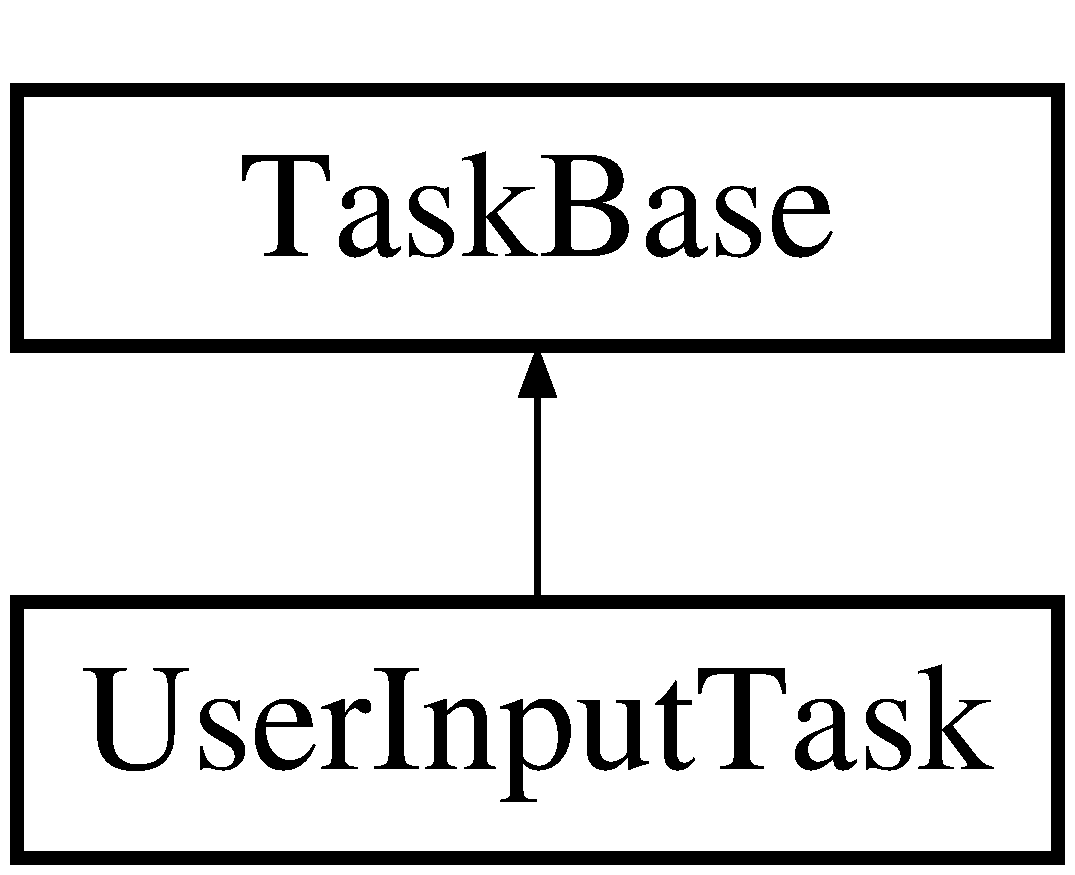
\includegraphics[height=2.000000cm]{class_user_input_task}
\end{center}
\end{figure}
\subsection*{Public Member Functions}
\begin{DoxyCompactItemize}
\item 
\mbox{\hyperlink{class_user_input_task_a46e07c6b7e8d143761f8a747c80a73f3}{User\+Input\+Task}} (const char $\ast$a\+\_\+name, unsigned port\+B\+A\+S\+E\+\_\+\+T\+Y\+PE a\+\_\+priority, size\+\_\+t a\+\_\+stack\+\_\+size, \mbox{\hyperlink{classemstream}{emstream}} $\ast$p\+\_\+ser\+\_\+dev)
\begin{DoxyCompactList}\small\item\em Construct a User\+Input task. \end{DoxyCompactList}\item 
void \mbox{\hyperlink{class_user_input_task_a03666bddf33829bd1eb0dfcfd7f7075b}{run}} (void)
\begin{DoxyCompactList}\small\item\em The run method of the User\+Input task that is repeatedly called by the R\+T\+OS scheduler. \end{DoxyCompactList}\end{DoxyCompactItemize}
\subsection*{Additional Inherited Members}


\subsection{Detailed Description}
Implements a task to determine the set-\/point of the ball on the beam. 

This class is an extension of {\ttfamily \mbox{\hyperlink{class_task_base}{Task\+Base}}}. The purpose of the class is to allow the user to interactively define the set-\/point of the ball by touching a linear resistive strip. 

\subsection{Constructor \& Destructor Documentation}
\mbox{\Hypertarget{class_user_input_task_a46e07c6b7e8d143761f8a747c80a73f3}\label{class_user_input_task_a46e07c6b7e8d143761f8a747c80a73f3}} 
\index{User\+Input\+Task@{User\+Input\+Task}!User\+Input\+Task@{User\+Input\+Task}}
\index{User\+Input\+Task@{User\+Input\+Task}!User\+Input\+Task@{User\+Input\+Task}}
\subsubsection{\texorpdfstring{User\+Input\+Task()}{UserInputTask()}}
{\footnotesize\ttfamily User\+Input\+Task\+::\+User\+Input\+Task (\begin{DoxyParamCaption}\item[{const char $\ast$}]{a\+\_\+name,  }\item[{unsigned port\+B\+A\+S\+E\+\_\+\+T\+Y\+PE}]{a\+\_\+priority,  }\item[{size\+\_\+t}]{a\+\_\+stack\+\_\+size,  }\item[{\mbox{\hyperlink{classemstream}{emstream}} $\ast$}]{p\+\_\+ser\+\_\+dev }\end{DoxyParamCaption})}



Construct a User\+Input task. 

Constructor which creates and initializes a User\+Interface task object.

This constructor sets up the task name, priority, stack size, and serial stream. 
\begin{DoxyParams}{Parameters}
{\em a\+\_\+name} & A character string which will be the name of this task \\
\hline
{\em a\+\_\+priority} & The priority at which this task will initially run (default\+: 0) \\
\hline
{\em a\+\_\+stack\+\_\+size} & The size of this task\textquotesingle{}s stack in bytes (default\+: {\ttfamily config\+M\+I\+N\+I\+M\+A\+L\+\_\+\+S\+T\+A\+C\+K\+\_\+\+S\+I\+ZE}) \\
\hline
{\em p\+\_\+ser\+\_\+dev} & Pointer to a serial device (port, radio, SD card, etc.) which can be used by this task to communicate (default\+: N\+U\+LL)\\
\hline
\end{DoxyParams}
This constructor creates a Free\+R\+T\+OS task with the given task run function, name, priority, and stack size. Its purpose is to determine the ball position setpoint based on the User\+Input sensor measurement. 
\begin{DoxyParams}{Parameters}
{\em a\+\_\+name} & A character string which will be the name of this task \\
\hline
{\em a\+\_\+priority} & The priority at which this task will initially run (default\+: 0) \\
\hline
{\em a\+\_\+stack\+\_\+size} & The size of this task\textquotesingle{}s stack in bytes (default\+: {\ttfamily config\+M\+I\+N\+I\+M\+A\+L\+\_\+\+S\+T\+A\+C\+K\+\_\+\+S\+I\+ZE}) \\
\hline
{\em p\+\_\+ser\+\_\+dev} & Pointer to a serial device (port, radio, SD card, etc.) which can be used by this task to communicate (default\+: N\+U\+LL) \\
\hline
\end{DoxyParams}


\subsection{Member Function Documentation}
\mbox{\Hypertarget{class_user_input_task_a03666bddf33829bd1eb0dfcfd7f7075b}\label{class_user_input_task_a03666bddf33829bd1eb0dfcfd7f7075b}} 
\index{User\+Input\+Task@{User\+Input\+Task}!run@{run}}
\index{run@{run}!User\+Input\+Task@{User\+Input\+Task}}
\subsubsection{\texorpdfstring{run()}{run()}}
{\footnotesize\ttfamily void User\+Input\+Task\+::run (\begin{DoxyParamCaption}\item[{void}]{ }\end{DoxyParamCaption})\hspace{0.3cm}{\ttfamily [virtual]}}



The run method of the User\+Input task that is repeatedly called by the R\+T\+OS scheduler. 

The {\ttfamily \mbox{\hyperlink{class_user_input_task_a03666bddf33829bd1eb0dfcfd7f7075b}{run()}}} function for the User\+Interface task.

This method is called by the R\+T\+OS scheduler. The function converts the linear potentiometer measurements to user position in m and user velocity in m/s. Shared variables are updated after the calculations are performed. 

Implements \mbox{\hyperlink{class_task_base_adcf6036ad9c860051ccf392ba5e7dbbc}{Task\+Base}}.



The documentation for this class was generated from the following files\+:\begin{DoxyCompactItemize}
\item 
Doxygen\+Files/\mbox{\hyperlink{_user_input_task_8h}{User\+Input\+Task.\+h}}\item 
Doxygen\+Files/User\+Input\+Task.\+cpp\end{DoxyCompactItemize}

\chapter{File Documentation}
\hypertarget{_ball_position_task_8h}{}\section{Doxygen\+Files/\+Ball\+Position\+Task.h File Reference}
\label{_ball_position_task_8h}\index{Doxygen\+Files/\+Ball\+Position\+Task.\+h@{Doxygen\+Files/\+Ball\+Position\+Task.\+h}}


Determines the ball position and velocity.  


{\ttfamily \#include \char`\"{}main.\+h\char`\"{}}\newline
{\ttfamily \#include \char`\"{}stm32l4xx\+\_\+hal.\+h\char`\"{}}\newline
{\ttfamily \#include \char`\"{}taskbase.\+h\char`\"{}}\newline
{\ttfamily \#include \char`\"{}taskqueue.\+h\char`\"{}}\newline
{\ttfamily \#include \char`\"{}taskshare.\+h\char`\"{}}\newline
{\ttfamily \#include \char`\"{}emstream.\+h\char`\"{}}\newline
\subsection*{Classes}
\begin{DoxyCompactItemize}
\item 
class \mbox{\hyperlink{class_ball_position_task}{Ball\+Position\+Task}}
\begin{DoxyCompactList}\small\item\em Implements a task to determine the ball position. \end{DoxyCompactList}\end{DoxyCompactItemize}


\subsection{Detailed Description}
Determines the ball position and velocity. 

This file defines the constructor and run method for the Ball\+Position task.

Revised\+: \begin{DoxyItemize}
\item 12-\/08-\/2018 J\+AT Original file \end{DoxyItemize}

\hypertarget{baseshare_8h}{}\section{Doxygen\+Files/baseshare.h File Reference}
\label{baseshare_8h}\index{Doxygen\+Files/baseshare.\+h@{Doxygen\+Files/baseshare.\+h}}


Source code of a base class for type-\/safe, thread-\/safe task data exchange classes.  


{\ttfamily \#include \char`\"{}Free\+R\+T\+O\+S.\+h\char`\"{}}\newline
{\ttfamily \#include \char`\"{}emstream.\+h\char`\"{}}\newline
\subsection*{Classes}
\begin{DoxyCompactItemize}
\item 
class \mbox{\hyperlink{class_base_share}{Base\+Share}}
\begin{DoxyCompactList}\small\item\em Base class for classes that share data in a thread-\/safe manner between tasks. \end{DoxyCompactList}\end{DoxyCompactItemize}


\subsection{Detailed Description}
Source code of a base class for type-\/safe, thread-\/safe task data exchange classes. 

Headers for a base class for type-\/safe, thread-\/safe task data exchange classes.

This file contains a base class for classes which exchange data between tasks. Inter-\/task data must be exchanged in a thread-\/safe manner, so the classes which share the data use mutexes or mutual exclusion mechanisms to prevent corruption of data. A linked list of all inter-\/task data items is kept by the M\+E405 system, and this base class contains members that handle that linked list.

Revised\+: \begin{DoxyItemize}
\item 10-\/18-\/2014 J\+RR Created file\end{DoxyItemize}
License\+: This file is copyright 2014 by JR Ridgely and released under the Lesser G\+NU Public License, version 2. It intended for educational use only, but its use is not limited thereto. 
\hypertarget{_controller_task_8h}{}\section{Doxygen\+Files/\+Controller\+Task.h File Reference}
\label{_controller_task_8h}\index{Doxygen\+Files/\+Controller\+Task.\+h@{Doxygen\+Files/\+Controller\+Task.\+h}}


Implements a state space control algorithm.  


{\ttfamily \#include \char`\"{}main.\+h\char`\"{}}\newline
{\ttfamily \#include \char`\"{}stm32l4xx\+\_\+hal.\+h\char`\"{}}\newline
{\ttfamily \#include \char`\"{}taskbase.\+h\char`\"{}}\newline
{\ttfamily \#include \char`\"{}taskqueue.\+h\char`\"{}}\newline
{\ttfamily \#include \char`\"{}taskshare.\+h\char`\"{}}\newline
{\ttfamily \#include \char`\"{}emstream.\+h\char`\"{}}\newline
\subsection*{Classes}
\begin{DoxyCompactItemize}
\item 
class \mbox{\hyperlink{class_controller_task}{Controller\+Task}}
\begin{DoxyCompactList}\small\item\em Implements a task to control the system. \end{DoxyCompactList}\end{DoxyCompactItemize}


\subsection{Detailed Description}
Implements a state space control algorithm. 

This file defines the constructor and run method for the controller task.

Revised\+: \begin{DoxyItemize}
\item 12-\/08-\/2018 J\+AT Original file \end{DoxyItemize}

\hypertarget{emstream_8cpp}{}\section{Doxygen\+Files/emstream.cpp File Reference}
\label{emstream_8cpp}\index{Doxygen\+Files/emstream.\+cpp@{Doxygen\+Files/emstream.\+cpp}}


Source code for a base class that imitates C++ I/O streams on serial devices.  


{\ttfamily \#include \char`\"{}emstream.\+h\char`\"{}}\newline
\subsection*{Functions}
\begin{DoxyCompactItemize}
\item 
\mbox{\hyperlink{emstream_8h_a5582483c459c0f48e51d96478d5b3407}{ser\+\_\+manipulator}} \mbox{\hyperlink{emstream_8cpp_a3c2c3d8ffc38044a12bdb9773cf9b7fa}{setprecision}} (uint8\+\_\+t digits)
\begin{DoxyCompactList}\small\item\em Set the number of digits shown after a decimal point. \end{DoxyCompactList}\item 
\mbox{\hyperlink{emstream_8h_a5582483c459c0f48e51d96478d5b3407}{ser\+\_\+manipulator}} \mbox{\hyperlink{emstream_8cpp_a1289b0bc61ac6556b4a891adbfa68bfe}{setbase}} (uint8\+\_\+t new\+\_\+base)
\begin{DoxyCompactList}\small\item\em Set the base for subsequent numeric conversions. \end{DoxyCompactList}\end{DoxyCompactItemize}
\subsection*{Variables}
\begin{DoxyCompactItemize}
\item 
uint8\+\_\+t \mbox{\hyperlink{emstream_8cpp_af2db72bc7e1c0c5ab90a66810114a029}{bts\+\_\+new\+\_\+prec}} = 3
\begin{DoxyCompactList}\small\item\em Temporary holder for {\ttfamily \mbox{\hyperlink{emstream_8cpp_a3c2c3d8ffc38044a12bdb9773cf9b7fa}{setprecision()}}} format function. \end{DoxyCompactList}\item 
uint8\+\_\+t \mbox{\hyperlink{emstream_8cpp_aea069c7881b86d9c2639c9ff51f3f5a7}{bts\+\_\+new\+\_\+base}} = 10
\begin{DoxyCompactList}\small\item\em Temporary holder for the {\ttfamily \mbox{\hyperlink{emstream_8cpp_a1289b0bc61ac6556b4a891adbfa68bfe}{setbase()}}} format function. \end{DoxyCompactList}\end{DoxyCompactItemize}


\subsection{Detailed Description}
Source code for a base class that imitates C++ I/O streams on serial devices. 

This file contains a base class for devices which send information in text form over serial devices. Example devices are serial ports (both traditional R\+S-\/232 ports and U\+S\+B-\/serial adapters) and wireless modems.

Revised\+: \begin{DoxyItemize}
\item 04-\/03-\/2006 J\+RR For updated version of compiler \item 06-\/10-\/2006 J\+RR Ported from C++ to C for use with some C-\/only projects \item 08-\/11-\/2006 J\+RR Some bug fixes \item 03-\/02-\/2007 J\+RR Ported back to C++. I\textquotesingle{}ve had it with the limitations of C. \item 04-\/16-\/2007 JO Added write (unsigned long) \item 07-\/19-\/2007 J\+RR Changed some character return values to bool, added m324p \item 01-\/12-\/2008 J\+RR Added code for the A\+Tmega128 using U\+S\+A\+RT number 1 only \item 02-\/13-\/2008 J\+RR Split into base class and device specific classes; changed from write() to overloaded $<$$<$ operator in the \char`\"{}cout\char`\"{} style \item 05-\/12-\/2008 A\+LS Fixed bug in which signed numbers came out unsigned \item 07-\/05-\/2008 J\+RR Added configuration macro by which to change what \char`\"{}endl\char`\"{} is \item 07-\/05-\/2008 J\+RR Added \textquotesingle{}ascii\textquotesingle{} and \textquotesingle{}numeric\textquotesingle{} format codes \item 11-\/24-\/2009 J\+RR Changed operation of \textquotesingle{}clrscr\textquotesingle{} to a function to work with L\+CD \item 11-\/26-\/2009 J\+RR Integrated floating point support into this file \item 12-\/16-\/2009 J\+RR Improved support for constant strings in program memory \item 10-\/22-\/2012 J\+RR Fixed (OK, hacked around) bug which caused spurious warning for all Program Memory Strings \item 11-\/12-\/2012 J\+RR Made puts() non-\/virtual; made \mbox{\hyperlink{emstream_8h_ae9ed5f0c8d6cc2b224363baf5157750d}{E\+N\+D\+L\+\_\+\+S\+T\+Y\+L\+E()}} a function macro \item 12-\/21-\/2013 J\+RR Ported to Chibi\+OS \item 10-\/17-\/2014 J\+RR Made compatible with Free\+R\+T\+OS for Cal Poly class use\end{DoxyItemize}
License\+: This file released under the Lesser G\+NU Public License, version 2. This program is intended for educational use only, but it is not limited thereto. This code incorporates elements from Xmelkov\textquotesingle{}s ftoa\+\_\+engine.\+h, part of the avr-\/libc source, and users must accept and comply with the license of ftoa\+\_\+engine.\+h as well. See \mbox{\hyperlink{emstream_8h}{emstream.\+h}} for a copy of the relevant license terms. 

\subsection{Function Documentation}
\mbox{\Hypertarget{emstream_8cpp_a1289b0bc61ac6556b4a891adbfa68bfe}\label{emstream_8cpp_a1289b0bc61ac6556b4a891adbfa68bfe}} 
\index{emstream.\+cpp@{emstream.\+cpp}!setbase@{setbase}}
\index{setbase@{setbase}!emstream.\+cpp@{emstream.\+cpp}}
\subsubsection{\texorpdfstring{setbase()}{setbase()}}
{\footnotesize\ttfamily \mbox{\hyperlink{emstream_8h_a5582483c459c0f48e51d96478d5b3407}{ser\+\_\+manipulator}} setbase (\begin{DoxyParamCaption}\item[{uint8\+\_\+t}]{new\+\_\+base }\end{DoxyParamCaption})}



Set the base for subsequent numeric conversions. 

This function, not a member of class emstream, sets the global numeric base and then returns a manipulator which causes a serial object to change to that base. The new base is \char`\"{}sticky\char`\"{} in that its value persists until this function is called (or the manipulators {\ttfamily bin}, {\ttfamily oct}, {\ttfamily dec} or {\ttfamily hex} are used) to change it again. Setting the base automatically turns off raw binary printing mode. 
\begin{DoxyParams}{Parameters}
{\em new\+\_\+base} & A new value for the numeric base, as long as it\textquotesingle{}s from 2 to 16 \\
\hline
\end{DoxyParams}
\begin{DoxyReturn}{Returns}
The serial manipulator called {\ttfamily manip\+\_\+set\+\_\+base} 
\end{DoxyReturn}
\mbox{\Hypertarget{emstream_8cpp_a3c2c3d8ffc38044a12bdb9773cf9b7fa}\label{emstream_8cpp_a3c2c3d8ffc38044a12bdb9773cf9b7fa}} 
\index{emstream.\+cpp@{emstream.\+cpp}!setprecision@{setprecision}}
\index{setprecision@{setprecision}!emstream.\+cpp@{emstream.\+cpp}}
\subsubsection{\texorpdfstring{setprecision()}{setprecision()}}
{\footnotesize\ttfamily \mbox{\hyperlink{emstream_8h_a5582483c459c0f48e51d96478d5b3407}{ser\+\_\+manipulator}} setprecision (\begin{DoxyParamCaption}\item[{uint8\+\_\+t}]{digits }\end{DoxyParamCaption})}



Set the number of digits shown after a decimal point. 

This function sets the global precision value, then returns a manipulator which causes a serial object to change its floating point precision (the number of digits after the decimal point which will be printed). The new precision is \char`\"{}sticky\char`\"{} in that its value persists until this function is called again to change it again. 
\begin{DoxyParams}{Parameters}
{\em digits} & A new value for the number of digits after the decimal point; a maximum of 7 digits are allowed \\
\hline
\end{DoxyParams}
\begin{DoxyReturn}{Returns}
The serial manipulator called \char`\"{}manip\+\_\+set\+\_\+precision\char`\"{} 
\end{DoxyReturn}


\subsection{Variable Documentation}
\mbox{\Hypertarget{emstream_8cpp_aea069c7881b86d9c2639c9ff51f3f5a7}\label{emstream_8cpp_aea069c7881b86d9c2639c9ff51f3f5a7}} 
\index{emstream.\+cpp@{emstream.\+cpp}!bts\+\_\+new\+\_\+base@{bts\+\_\+new\+\_\+base}}
\index{bts\+\_\+new\+\_\+base@{bts\+\_\+new\+\_\+base}!emstream.\+cpp@{emstream.\+cpp}}
\subsubsection{\texorpdfstring{bts\+\_\+new\+\_\+base}{bts\_new\_base}}
{\footnotesize\ttfamily uint8\+\_\+t bts\+\_\+new\+\_\+base = 10}



Temporary holder for the {\ttfamily \mbox{\hyperlink{emstream_8cpp_a1289b0bc61ac6556b4a891adbfa68bfe}{setbase()}}} format function. 

This variable allows the nonmember function {\ttfamily \mbox{\hyperlink{emstream_8cpp_a1289b0bc61ac6556b4a891adbfa68bfe}{setbase()}}} to communicate a new numeric base to a specific serial device object. The {\ttfamily \mbox{\hyperlink{emstream_8cpp_a1289b0bc61ac6556b4a891adbfa68bfe}{setbase()}}} method returns a manipulator that causes a specific serial object (the one in whose {\ttfamily cout} style output line it is called) to read the value of this variable. \mbox{\Hypertarget{emstream_8cpp_af2db72bc7e1c0c5ab90a66810114a029}\label{emstream_8cpp_af2db72bc7e1c0c5ab90a66810114a029}} 
\index{emstream.\+cpp@{emstream.\+cpp}!bts\+\_\+new\+\_\+prec@{bts\+\_\+new\+\_\+prec}}
\index{bts\+\_\+new\+\_\+prec@{bts\+\_\+new\+\_\+prec}!emstream.\+cpp@{emstream.\+cpp}}
\subsubsection{\texorpdfstring{bts\+\_\+new\+\_\+prec}{bts\_new\_prec}}
{\footnotesize\ttfamily uint8\+\_\+t bts\+\_\+new\+\_\+prec = 3}



Temporary holder for {\ttfamily \mbox{\hyperlink{emstream_8cpp_a3c2c3d8ffc38044a12bdb9773cf9b7fa}{setprecision()}}} format function. 

This variable allows the nonmember function {\ttfamily \mbox{\hyperlink{emstream_8cpp_a3c2c3d8ffc38044a12bdb9773cf9b7fa}{setprecision()}}} to communicate the number of digits after the decimal point to a specific text serial port object. The {\ttfamily \mbox{\hyperlink{emstream_8cpp_a3c2c3d8ffc38044a12bdb9773cf9b7fa}{setprecision()}}} function returns a manipulator that causes a specific serial object (the one in whose {\ttfamily cout} style output line it is called) to read the value of this variable. 
\hypertarget{emstream_8h}{}\section{Doxygen\+Files/emstream.h File Reference}
\label{emstream_8h}\index{Doxygen\+Files/emstream.\+h@{Doxygen\+Files/emstream.\+h}}


Headers for a base class that imitates C++ I/O streams on serial devices.  


{\ttfamily \#include $<$stdint.\+h$>$}\newline
\subsection*{Classes}
\begin{DoxyCompactItemize}
\item 
class \mbox{\hyperlink{classemstream}{emstream}}
\begin{DoxyCompactList}\small\item\em Base class for serial devices which print using a {\ttfamily $<$$<$} operator. \end{DoxyCompactList}\end{DoxyCompactItemize}
\subsection*{Macros}
\begin{DoxyCompactItemize}
\item 
\#define \mbox{\hyperlink{emstream_8h_ae9ed5f0c8d6cc2b224363baf5157750d}{E\+N\+D\+L\+\_\+\+S\+T\+Y\+LE}}()~putchar (\textquotesingle{}\textbackslash{}r\textquotesingle{}); putchar (\textquotesingle{}\textbackslash{}n\textquotesingle{})
\begin{DoxyCompactList}\small\item\em This define selects what will be sent when a program sends out \char`\"{}endl\char`\"{}. \end{DoxyCompactList}\item 
\#define \mbox{\hyperlink{emstream_8h_addb19a39c5f07b2af76670f678f70661}{C\+L\+R\+S\+C\+R\+\_\+\+S\+T\+Y\+LE}}~\char`\"{}\textbackslash{}033\mbox{[}2\+J\textbackslash{}033\mbox{[}\+H\char`\"{}
\begin{DoxyCompactList}\small\item\em This define selects the character which asks a terminal to clear its screen. \end{DoxyCompactList}\item 
\#define \mbox{\hyperlink{emstream_8h_a076d1892c2e1133e4cc5469015af6423}{P\+MS}}(s)~s
\begin{DoxyCompactList}\small\item\em This define allows strings to be kept in A\+VR program (flash) memory only. \end{DoxyCompactList}\item 
\#define \mbox{\hyperlink{emstream_8h_a14df2aae4c89a3755b2ae48e55172e90}{D\+BG}}(ptr,  stuff)
\begin{DoxyCompactList}\small\item\em This macro simplifies the writing of code to conditionally print debugging output. \end{DoxyCompactList}\end{DoxyCompactItemize}
\subsection*{Enumerations}
\begin{DoxyCompactItemize}
\item 
enum \mbox{\hyperlink{emstream_8h_a5582483c459c0f48e51d96478d5b3407}{ser\+\_\+manipulator}} \{ \newline
\mbox{\hyperlink{emstream_8h_a5582483c459c0f48e51d96478d5b3407ad843ac028b91abce26e3d42b2e27eae0}{bin}}, 
\mbox{\hyperlink{emstream_8h_a5582483c459c0f48e51d96478d5b3407a8f2c05194d91776b033f24e214c6e9df}{oct}}, 
\mbox{\hyperlink{emstream_8h_a5582483c459c0f48e51d96478d5b3407a82022a5c9021c54619b7b00d1fede0ad}{dec}}, 
\mbox{\hyperlink{emstream_8h_a5582483c459c0f48e51d96478d5b3407a6000f7a8e67e4e0beb7b8ebe93452243}{hex}}, 
\newline
\mbox{\hyperlink{emstream_8h_a5582483c459c0f48e51d96478d5b3407aca212f0f54e5a7620d5622be097d7db9}{roman}}, 
{\bfseries fortran}, 
\mbox{\hyperlink{emstream_8h_a5582483c459c0f48e51d96478d5b3407a5cbad4ad24fd9b8c066cdad096cd2f18}{endl}}, 
\mbox{\hyperlink{emstream_8h_a5582483c459c0f48e51d96478d5b3407ab6ca2a7533366acce99cc85a1da20008}{clrscr}}, 
\newline
\mbox{\hyperlink{emstream_8h_a5582483c459c0f48e51d96478d5b3407a90718791e807ebb8af4ebc39df0b98f7}{send\+\_\+now}}, 
\mbox{\hyperlink{emstream_8h_a5582483c459c0f48e51d96478d5b3407a2b6bb413c07a0678c5603fde1bb7226f}{manip\+\_\+set\+\_\+precision}}, 
\mbox{\hyperlink{emstream_8h_a5582483c459c0f48e51d96478d5b3407a1d29fa0ebfea9229dbb90393c9f123d4}{manip\+\_\+set\+\_\+base}}, 
\mbox{\hyperlink{emstream_8h_a5582483c459c0f48e51d96478d5b3407aa6ac72a2e8fdb9465c683bcf0db34c5d}{manip\+\_\+do\+\_\+nothing}}
 \}
\begin{DoxyCompactList}\small\item\em Modifiers used to adjust how things are printed with the {\ttfamily $<$$<$} operator. \end{DoxyCompactList}\end{DoxyCompactItemize}
\subsection*{Functions}
\begin{DoxyCompactItemize}
\item 
\mbox{\hyperlink{emstream_8h_a5582483c459c0f48e51d96478d5b3407}{ser\+\_\+manipulator}} \mbox{\hyperlink{emstream_8h_a190348e5180d4e7481a23ce12b22fcce}{setprecision}} (uint8\+\_\+t)
\begin{DoxyCompactList}\small\item\em Set the number of digits shown after a decimal point. \end{DoxyCompactList}\item 
\mbox{\hyperlink{emstream_8h_a5582483c459c0f48e51d96478d5b3407}{ser\+\_\+manipulator}} \mbox{\hyperlink{emstream_8h_a1289b0bc61ac6556b4a891adbfa68bfe}{setbase}} (uint8\+\_\+t new\+\_\+base)
\begin{DoxyCompactList}\small\item\em Set the base for subsequent numeric conversions. \end{DoxyCompactList}\item 
\mbox{\Hypertarget{emstream_8h_a62500c4d5d1ea781a91d6bd1689987d1}\label{emstream_8h_a62500c4d5d1ea781a91d6bd1689987d1}} 
void {\bfseries hex\+\_\+dump\+\_\+memory} (uint8\+\_\+t $\ast$, uint8\+\_\+t $\ast$, \mbox{\hyperlink{classemstream}{emstream}} $\ast$)
\end{DoxyCompactItemize}
\subsection*{Variables}
\begin{DoxyCompactItemize}
\item 
const char \mbox{\hyperlink{emstream_8h_a9fe209e5a772772badf2085562677114}{E\+M\+S\+T\+R\+\_\+\+A\+S\+C\+I\+I\+\_\+\+C\+H\+A\+RS}} \mbox{[}$\,$\mbox{]} = \char`\"{}F\+E\+D\+C\+B\+A9876543210123456789\+A\+B\+C\+D\+EF\char`\"{}
\begin{DoxyCompactList}\small\item\em String of characters used to convert numbers into printable characters. \end{DoxyCompactList}\end{DoxyCompactItemize}


\subsection{Detailed Description}
Headers for a base class that imitates C++ I/O streams on serial devices. 

This file contains a base class for devices which send information in text form over serial devices. Example devices are serial ports (both traditional R\+S-\/232 ports and U\+S\+B-\/serial adapters) and wireless modems.

Revised\+: \begin{DoxyItemize}
\item 04-\/03-\/2006 J\+RR For updated version of compiler \item 06-\/10-\/2006 J\+RR Ported from C++ to C for use with some C-\/only projects \item 08-\/11-\/2006 J\+RR Some bug fixes \item 03-\/02-\/2007 J\+RR Ported back to C++. I\textquotesingle{}ve had it with the limitations of C. \item 04-\/16-\/2007 JO Added write (unsigned long) \item 07-\/19-\/2007 J\+RR Changed some character return values to bool, added m324p \item 01-\/12-\/2008 J\+RR Added code for the A\+Tmega128 using U\+S\+A\+RT number 1 only \item 02-\/13-\/2008 J\+RR Split into base class and device specific classes; changed from write() to overloaded $<$$<$ operator in the \char`\"{}cout\char`\"{} style \item 05-\/12-\/2008 A\+LS Fixed bug in which signed numbers came out unsigned \item 07-\/05-\/2008 J\+RR Added configuration macro by which to change what \char`\"{}endl\char`\"{} is \item 07-\/05-\/2008 J\+RR Added \textquotesingle{}ascii\textquotesingle{} and \textquotesingle{}numeric\textquotesingle{} format codes \item 11-\/24-\/2009 J\+RR Changed operation of \textquotesingle{}clrscr\textquotesingle{} to a function to work with L\+CD \item 11-\/26-\/2009 J\+RR Integrated floating point support into this file \item 12-\/16-\/2009 J\+RR Improved support for constant strings in program memory \item 10-\/22-\/2012 J\+RR Fixed (OK, hacked around) bug which caused spurious warning for all Program Memory Strings \item 11-\/12-\/2012 J\+RR Made puts() non-\/virtual; made \mbox{\hyperlink{emstream_8h_ae9ed5f0c8d6cc2b224363baf5157750d}{E\+N\+D\+L\+\_\+\+S\+T\+Y\+L\+E()}} a function macro \item 12-\/21-\/2013 J\+RR Ported to Chibi\+OS \item 10-\/17-\/2014 J\+RR Made compatible with Free\+R\+T\+OS for Cal Poly class use\end{DoxyItemize}
License\+: This file released under the Lesser G\+NU Public License, version 2. This program is intended for educational use only, but it is not limited thereto. This code incorporates elements from Xmelkov\textquotesingle{}s ftoa\+\_\+engine.\+h, part of the avr-\/libc source, and users must accept and comply with the license of ftoa\+\_\+engine.\+h as well. 

\subsection{Macro Definition Documentation}
\mbox{\Hypertarget{emstream_8h_addb19a39c5f07b2af76670f678f70661}\label{emstream_8h_addb19a39c5f07b2af76670f678f70661}} 
\index{emstream.\+h@{emstream.\+h}!C\+L\+R\+S\+C\+R\+\_\+\+S\+T\+Y\+LE@{C\+L\+R\+S\+C\+R\+\_\+\+S\+T\+Y\+LE}}
\index{C\+L\+R\+S\+C\+R\+\_\+\+S\+T\+Y\+LE@{C\+L\+R\+S\+C\+R\+\_\+\+S\+T\+Y\+LE}!emstream.\+h@{emstream.\+h}}
\subsubsection{\texorpdfstring{C\+L\+R\+S\+C\+R\+\_\+\+S\+T\+Y\+LE}{CLRSCR\_STYLE}}
{\footnotesize\ttfamily \#define C\+L\+R\+S\+C\+R\+\_\+\+S\+T\+Y\+LE~\char`\"{}\textbackslash{}033\mbox{[}2\+J\textbackslash{}033\mbox{[}\+H\char`\"{}}



This define selects the character which asks a terminal to clear its screen. 

The clear-\/screen character for an A\+N\+S\+II standard terminal is a control-\/L, which is A\+S\+C\+II character number 12. \mbox{\Hypertarget{emstream_8h_a14df2aae4c89a3755b2ae48e55172e90}\label{emstream_8h_a14df2aae4c89a3755b2ae48e55172e90}} 
\index{emstream.\+h@{emstream.\+h}!D\+BG@{D\+BG}}
\index{D\+BG@{D\+BG}!emstream.\+h@{emstream.\+h}}
\subsubsection{\texorpdfstring{D\+BG}{DBG}}
{\footnotesize\ttfamily \#define D\+BG(\begin{DoxyParamCaption}\item[{}]{ptr,  }\item[{}]{stuff }\end{DoxyParamCaption})}



This macro simplifies the writing of code to conditionally print debugging output. 

If S\+E\+R\+I\+A\+L\+\_\+\+D\+E\+B\+UG hasn\textquotesingle{}t been defined, it replaces a debugging command with nothing.

If S\+E\+R\+I\+A\+L\+\_\+\+D\+E\+B\+UG has been defined, it drops in a command that checks the given serial device pointer to make sure the device isn\textquotesingle{}t N\+U\+LL, and if the device isn\textquotesingle{}t N\+U\+LL then debugging output is printed. \mbox{\Hypertarget{emstream_8h_ae9ed5f0c8d6cc2b224363baf5157750d}\label{emstream_8h_ae9ed5f0c8d6cc2b224363baf5157750d}} 
\index{emstream.\+h@{emstream.\+h}!E\+N\+D\+L\+\_\+\+S\+T\+Y\+LE@{E\+N\+D\+L\+\_\+\+S\+T\+Y\+LE}}
\index{E\+N\+D\+L\+\_\+\+S\+T\+Y\+LE@{E\+N\+D\+L\+\_\+\+S\+T\+Y\+LE}!emstream.\+h@{emstream.\+h}}
\subsubsection{\texorpdfstring{E\+N\+D\+L\+\_\+\+S\+T\+Y\+LE}{ENDL\_STYLE}}
{\footnotesize\ttfamily \#define E\+N\+D\+L\+\_\+\+S\+T\+Y\+LE(\begin{DoxyParamCaption}{ }\end{DoxyParamCaption})~putchar (\textquotesingle{}\textbackslash{}r\textquotesingle{}); putchar (\textquotesingle{}\textbackslash{}n\textquotesingle{})}



This define selects what will be sent when a program sends out \char`\"{}endl\char`\"{}. 

Different recieving programs want different end-\/of-\/line markers. Traditionally, U\+N\+IX uses \char`\"{}\textbackslash{}r\char`\"{} while PC\textquotesingle{}s use \char`\"{}\textbackslash{}r\textbackslash{}n\char`\"{} and Macs use \char`\"{}\textbackslash{}n\char`\"{} (I think). \mbox{\Hypertarget{emstream_8h_a076d1892c2e1133e4cc5469015af6423}\label{emstream_8h_a076d1892c2e1133e4cc5469015af6423}} 
\index{emstream.\+h@{emstream.\+h}!P\+MS@{P\+MS}}
\index{P\+MS@{P\+MS}!emstream.\+h@{emstream.\+h}}
\subsubsection{\texorpdfstring{P\+MS}{PMS}}
{\footnotesize\ttfamily \#define P\+MS(\begin{DoxyParamCaption}\item[{}]{s }\end{DoxyParamCaption})~s}



This define allows strings to be kept in A\+VR program (flash) memory only. 

It tells the puts() method to find them in program memory. This saves S\+R\+AM memory compared to copying all the strings to S\+R\+AM, which is the rather wasteful default method used by the compiler. See the following link for more information about strings in program memory\+: \begin{DoxyItemize}
\item \href{http://www.avrfreaks.net/index.php?name=PNphpBB2&file=viewtopic&t=57011}{\tt http\+://www.\+avrfreaks.\+net/index.\+php?name=\+P\+Nphp\+B\+B2\&file=viewtopic\&t=57011} \end{DoxyItemize}


\subsection{Enumeration Type Documentation}
\mbox{\Hypertarget{emstream_8h_a5582483c459c0f48e51d96478d5b3407}\label{emstream_8h_a5582483c459c0f48e51d96478d5b3407}} 
\index{emstream.\+h@{emstream.\+h}!ser\+\_\+manipulator@{ser\+\_\+manipulator}}
\index{ser\+\_\+manipulator@{ser\+\_\+manipulator}!emstream.\+h@{emstream.\+h}}
\subsubsection{\texorpdfstring{ser\+\_\+manipulator}{ser\_manipulator}}
{\footnotesize\ttfamily enum \mbox{\hyperlink{emstream_8h_a5582483c459c0f48e51d96478d5b3407}{ser\+\_\+manipulator}}}



Modifiers used to adjust how things are printed with the {\ttfamily $<$$<$} operator. 

This enumeration is used to modify the way in which various things are printed by descendent classes of {\ttfamily emstream} and to insert special characters into what is being printed out. Values can change the display base for the output stream from the default of base 10 (decimal) to and from any base between 2 (binary), and 16 (hexadecimal), inclusive. The precision for printing floating point numbers can be adjusted with {\bfseries \mbox{\hyperlink{emstream_8h_a190348e5180d4e7481a23ce12b22fcce}{setprecision()}}}, which emits the {\ttfamily manip\+\_\+set\+\_\+precision} modifier. Also defined are {\ttfamily endl} to send an end-\/of-\/line character, {\ttfamily clrscr} to send a clear-\/screen character which works with some terminal emulators and not others, and {\ttfamily send\+\_\+now} to tell some devices to transmit data as soon as possible. \begin{DoxyEnumFields}{Enumerator}
\raisebox{\heightof{T}}[0pt][0pt]{\index{bin@{bin}!emstream.\+h@{emstream.\+h}}\index{emstream.\+h@{emstream.\+h}!bin@{bin}}}\mbox{\Hypertarget{emstream_8h_a5582483c459c0f48e51d96478d5b3407ad843ac028b91abce26e3d42b2e27eae0}\label{emstream_8h_a5582483c459c0f48e51d96478d5b3407ad843ac028b91abce26e3d42b2e27eae0}} 
bin&Print following numbers in base 2 (binary) until another base is specified. \\
\hline

\raisebox{\heightof{T}}[0pt][0pt]{\index{oct@{oct}!emstream.\+h@{emstream.\+h}}\index{emstream.\+h@{emstream.\+h}!oct@{oct}}}\mbox{\Hypertarget{emstream_8h_a5582483c459c0f48e51d96478d5b3407a8f2c05194d91776b033f24e214c6e9df}\label{emstream_8h_a5582483c459c0f48e51d96478d5b3407a8f2c05194d91776b033f24e214c6e9df}} 
oct&Print following numbers in base 8 (octal) until another base is specified. \\
\hline

\raisebox{\heightof{T}}[0pt][0pt]{\index{dec@{dec}!emstream.\+h@{emstream.\+h}}\index{emstream.\+h@{emstream.\+h}!dec@{dec}}}\mbox{\Hypertarget{emstream_8h_a5582483c459c0f48e51d96478d5b3407a82022a5c9021c54619b7b00d1fede0ad}\label{emstream_8h_a5582483c459c0f48e51d96478d5b3407a82022a5c9021c54619b7b00d1fede0ad}} 
dec&Print following numbers in base 10 (decimal) until another base is specified. \\
\hline

\raisebox{\heightof{T}}[0pt][0pt]{\index{hex@{hex}!emstream.\+h@{emstream.\+h}}\index{emstream.\+h@{emstream.\+h}!hex@{hex}}}\mbox{\Hypertarget{emstream_8h_a5582483c459c0f48e51d96478d5b3407a6000f7a8e67e4e0beb7b8ebe93452243}\label{emstream_8h_a5582483c459c0f48e51d96478d5b3407a6000f7a8e67e4e0beb7b8ebe93452243}} 
hex&Print following numbers in base 16 (hexadecimal) until another base is specified. \\
\hline

\raisebox{\heightof{T}}[0pt][0pt]{\index{roman@{roman}!emstream.\+h@{emstream.\+h}}\index{emstream.\+h@{emstream.\+h}!roman@{roman}}}\mbox{\Hypertarget{emstream_8h_a5582483c459c0f48e51d96478d5b3407aca212f0f54e5a7620d5622be097d7db9}\label{emstream_8h_a5582483c459c0f48e51d96478d5b3407aca212f0f54e5a7620d5622be097d7db9}} 
roman&Print following integers in Roman numerals rather than Arabic. \\
\hline

\raisebox{\heightof{T}}[0pt][0pt]{\index{endl@{endl}!emstream.\+h@{emstream.\+h}}\index{emstream.\+h@{emstream.\+h}!endl@{endl}}}\mbox{\Hypertarget{emstream_8h_a5582483c459c0f48e51d96478d5b3407a5cbad4ad24fd9b8c066cdad096cd2f18}\label{emstream_8h_a5582483c459c0f48e51d96478d5b3407a5cbad4ad24fd9b8c066cdad096cd2f18}} 
endl&Print a carriage return and/or linefeed as specified in {\ttfamily E\+N\+D\+L\+\_\+\+S\+T\+Y\+LE}. \\
\hline

\raisebox{\heightof{T}}[0pt][0pt]{\index{clrscr@{clrscr}!emstream.\+h@{emstream.\+h}}\index{emstream.\+h@{emstream.\+h}!clrscr@{clrscr}}}\mbox{\Hypertarget{emstream_8h_a5582483c459c0f48e51d96478d5b3407ab6ca2a7533366acce99cc85a1da20008}\label{emstream_8h_a5582483c459c0f48e51d96478d5b3407ab6ca2a7533366acce99cc85a1da20008}} 
clrscr&Send a character specified in {\ttfamily C\+L\+R\+S\+C\+R\+\_\+\+S\+T\+Y\+LE} to clear some terminal screens. \\
\hline

\raisebox{\heightof{T}}[0pt][0pt]{\index{send\+\_\+now@{send\+\_\+now}!emstream.\+h@{emstream.\+h}}\index{emstream.\+h@{emstream.\+h}!send\+\_\+now@{send\+\_\+now}}}\mbox{\Hypertarget{emstream_8h_a5582483c459c0f48e51d96478d5b3407a90718791e807ebb8af4ebc39df0b98f7}\label{emstream_8h_a5582483c459c0f48e51d96478d5b3407a90718791e807ebb8af4ebc39df0b98f7}} 
send\+\_\+now&If relevant to a device, tell it to send or save data immediately. \\
\hline

\raisebox{\heightof{T}}[0pt][0pt]{\index{manip\+\_\+set\+\_\+precision@{manip\+\_\+set\+\_\+precision}!emstream.\+h@{emstream.\+h}}\index{emstream.\+h@{emstream.\+h}!manip\+\_\+set\+\_\+precision@{manip\+\_\+set\+\_\+precision}}}\mbox{\Hypertarget{emstream_8h_a5582483c459c0f48e51d96478d5b3407a2b6bb413c07a0678c5603fde1bb7226f}\label{emstream_8h_a5582483c459c0f48e51d96478d5b3407a2b6bb413c07a0678c5603fde1bb7226f}} 
manip\+\_\+set\+\_\+precision&Set the precision (numbers after decimal) for printing floating point numbers. \\
\hline

\raisebox{\heightof{T}}[0pt][0pt]{\index{manip\+\_\+set\+\_\+base@{manip\+\_\+set\+\_\+base}!emstream.\+h@{emstream.\+h}}\index{emstream.\+h@{emstream.\+h}!manip\+\_\+set\+\_\+base@{manip\+\_\+set\+\_\+base}}}\mbox{\Hypertarget{emstream_8h_a5582483c459c0f48e51d96478d5b3407a1d29fa0ebfea9229dbb90393c9f123d4}\label{emstream_8h_a5582483c459c0f48e51d96478d5b3407a1d29fa0ebfea9229dbb90393c9f123d4}} 
manip\+\_\+set\+\_\+base&Set the numeric base in which to print numbers. \\
\hline

\raisebox{\heightof{T}}[0pt][0pt]{\index{manip\+\_\+do\+\_\+nothing@{manip\+\_\+do\+\_\+nothing}!emstream.\+h@{emstream.\+h}}\index{emstream.\+h@{emstream.\+h}!manip\+\_\+do\+\_\+nothing@{manip\+\_\+do\+\_\+nothing}}}\mbox{\Hypertarget{emstream_8h_a5582483c459c0f48e51d96478d5b3407aa6ac72a2e8fdb9465c683bcf0db34c5d}\label{emstream_8h_a5582483c459c0f48e51d96478d5b3407aa6ac72a2e8fdb9465c683bcf0db34c5d}} 
manip\+\_\+do\+\_\+nothing&Placeholder manipulator that causes nothing to happen. \\
\hline

\end{DoxyEnumFields}


\subsection{Function Documentation}
\mbox{\Hypertarget{emstream_8h_a1289b0bc61ac6556b4a891adbfa68bfe}\label{emstream_8h_a1289b0bc61ac6556b4a891adbfa68bfe}} 
\index{emstream.\+h@{emstream.\+h}!setbase@{setbase}}
\index{setbase@{setbase}!emstream.\+h@{emstream.\+h}}
\subsubsection{\texorpdfstring{setbase()}{setbase()}}
{\footnotesize\ttfamily \mbox{\hyperlink{emstream_8h_a5582483c459c0f48e51d96478d5b3407}{ser\+\_\+manipulator}} setbase (\begin{DoxyParamCaption}\item[{uint8\+\_\+t}]{new\+\_\+base }\end{DoxyParamCaption})}



Set the base for subsequent numeric conversions. 

This function, not a member of class emstream, sets the global numeric base and then returns a manipulator which causes a serial object to change to that base. The new base is \char`\"{}sticky\char`\"{} in that its value persists until this function is called (or the manipulators {\ttfamily bin}, {\ttfamily oct}, {\ttfamily dec} or {\ttfamily hex} are used) to change it again. Setting the base automatically turns off raw binary printing mode. 
\begin{DoxyParams}{Parameters}
{\em new\+\_\+base} & A new value for the numeric base, as long as it\textquotesingle{}s from 2 to 16 \\
\hline
\end{DoxyParams}
\begin{DoxyReturn}{Returns}
The serial manipulator called {\ttfamily manip\+\_\+set\+\_\+base} 
\end{DoxyReturn}
\mbox{\Hypertarget{emstream_8h_a190348e5180d4e7481a23ce12b22fcce}\label{emstream_8h_a190348e5180d4e7481a23ce12b22fcce}} 
\index{emstream.\+h@{emstream.\+h}!setprecision@{setprecision}}
\index{setprecision@{setprecision}!emstream.\+h@{emstream.\+h}}
\subsubsection{\texorpdfstring{setprecision()}{setprecision()}}
{\footnotesize\ttfamily \mbox{\hyperlink{emstream_8h_a5582483c459c0f48e51d96478d5b3407}{ser\+\_\+manipulator}} setprecision (\begin{DoxyParamCaption}\item[{uint8\+\_\+t}]{digits }\end{DoxyParamCaption})}



Set the number of digits shown after a decimal point. 

This function sets the global precision value, then returns a manipulator which causes a serial object to change its floating point precision (the number of digits after the decimal point which will be printed). The new precision is \char`\"{}sticky\char`\"{} in that its value persists until this function is called again to change it again. 
\begin{DoxyParams}{Parameters}
{\em digits} & A new value for the number of digits after the decimal point; a maximum of 7 digits are allowed \\
\hline
\end{DoxyParams}
\begin{DoxyReturn}{Returns}
The serial manipulator called \char`\"{}manip\+\_\+set\+\_\+precision\char`\"{} 
\end{DoxyReturn}


\subsection{Variable Documentation}
\mbox{\Hypertarget{emstream_8h_a9fe209e5a772772badf2085562677114}\label{emstream_8h_a9fe209e5a772772badf2085562677114}} 
\index{emstream.\+h@{emstream.\+h}!E\+M\+S\+T\+R\+\_\+\+A\+S\+C\+I\+I\+\_\+\+C\+H\+A\+RS@{E\+M\+S\+T\+R\+\_\+\+A\+S\+C\+I\+I\+\_\+\+C\+H\+A\+RS}}
\index{E\+M\+S\+T\+R\+\_\+\+A\+S\+C\+I\+I\+\_\+\+C\+H\+A\+RS@{E\+M\+S\+T\+R\+\_\+\+A\+S\+C\+I\+I\+\_\+\+C\+H\+A\+RS}!emstream.\+h@{emstream.\+h}}
\subsubsection{\texorpdfstring{E\+M\+S\+T\+R\+\_\+\+A\+S\+C\+I\+I\+\_\+\+C\+H\+A\+RS}{EMSTR\_ASCII\_CHARS}}
{\footnotesize\ttfamily const char E\+M\+S\+T\+R\+\_\+\+A\+S\+C\+I\+I\+\_\+\+C\+H\+A\+RS\mbox{[}$\,$\mbox{]} = \char`\"{}F\+E\+D\+C\+B\+A9876543210123456789\+A\+B\+C\+D\+EF\char`\"{}}



String of characters used to convert numbers into printable characters. 

This definition is used to allow variables of type {\ttfamily size\+\_\+t} to be somewhat conveniently transmitted by descendents of class {\ttfamily emstream}. One needs to put a typecast before each such variable, because the normal automatic type detection doesn\textquotesingle{}t always work for variables of type {\ttfamily size\+\_\+t}. The usage is {\ttfamily a\+\_\+serial\+\_\+device} {\ttfamily $<$$<$} {\ttfamily }(ems\+\_\+size\+\_\+t) {\ttfamily thing};

This string is used by functions in class {\ttfamily emstream} which convert numbers into sets of A\+S\+C\+II characters to be sent to serial devices. It allows the use of fairly efficient versions of {\ttfamily itoa()} and related functions which perform the translation through a simple table lookup. 
\hypertarget{emstream__bool_8cpp}{}\section{Doxygen\+Files/emstream\+\_\+bool.cpp File Reference}
\label{emstream__bool_8cpp}\index{Doxygen\+Files/emstream\+\_\+bool.\+cpp@{Doxygen\+Files/emstream\+\_\+bool.\+cpp}}
{\ttfamily \#include $<$stdlib.\+h$>$}\newline
{\ttfamily \#include \char`\"{}emstream.\+h\char`\"{}}\newline


\subsection{Detailed Description}
This file contains an operator which prints a Boolean value as either a \textquotesingle{}T\textquotesingle{} or a \textquotesingle{}F\textquotesingle{} using the {\ttfamily emstream} class.

Revised\+: \begin{DoxyItemize}
\item 12-\/02-\/2012 J\+RR Split this file off from the main {\ttfamily \mbox{\hyperlink{emstream_8cpp}{emstream.\+cpp}}} to allow smaller machine code if stuff in this file isn\textquotesingle{}t used\end{DoxyItemize}
License\+: This file released under the Lesser G\+NU Public License, version 2. This program is intended for educational use only, but it is not limited thereto. This code incorporates elements from Xmelkov\textquotesingle{}s ftoa\+\_\+engine.\+h, part of the avr-\/libc source, and users must accept and comply with the license of ftoa\+\_\+engine.\+h as well. See \mbox{\hyperlink{emstream_8h}{emstream.\+h}} for a copy of the relevant license terms. 
\hypertarget{emstream__float_8cpp}{}\section{Doxygen\+Files/emstream\+\_\+float.cpp File Reference}
\label{emstream__float_8cpp}\index{Doxygen\+Files/emstream\+\_\+float.\+cpp@{Doxygen\+Files/emstream\+\_\+float.\+cpp}}
{\ttfamily \#include $<$stdint.\+h$>$}\newline
{\ttfamily \#include $<$stdlib.\+h$>$}\newline
{\ttfamily \#include \char`\"{}emstream.\+h\char`\"{}}\newline
\subsection*{Classes}
\begin{DoxyCompactItemize}
\item 
union \mbox{\hyperlink{unionfloat__with__bits__t}{float\+\_\+with\+\_\+bits\+\_\+t}}
\begin{DoxyCompactList}\small\item\em Single precision float accessed as a float or a set of 32 bits. \end{DoxyCompactList}\end{DoxyCompactItemize}


\subsection{Detailed Description}
This file contains the operators which print floating-\/point numbers using the {\ttfamily emstream} class.

Revised\+: \begin{DoxyItemize}
\item 12-\/02-\/2012 J\+RR Split this file off from the main {\ttfamily \mbox{\hyperlink{emstream_8cpp}{emstream.\+cpp}}} to allow smaller machine code if stuff in this file isn\textquotesingle{}t used\end{DoxyItemize}
License\+: This file released under the Lesser G\+NU Public License, version 2. This program is intended for educational use only, but it is not limited thereto. This code incorporates elements from Xmelkov\textquotesingle{}s ftoa\+\_\+engine.\+h, part of the avr-\/libc source, and users must accept and comply with the license of ftoa\+\_\+engine.\+h as well. See \mbox{\hyperlink{emstream_8h}{emstream.\+h}} for a copy of the relevant license terms. 
\hypertarget{emstream__int16__t_8cpp}{}\section{Doxygen\+Files/emstream\+\_\+int16\+\_\+t.cpp File Reference}
\label{emstream__int16__t_8cpp}\index{Doxygen\+Files/emstream\+\_\+int16\+\_\+t.\+cpp@{Doxygen\+Files/emstream\+\_\+int16\+\_\+t.\+cpp}}
{\ttfamily \#include $<$stdlib.\+h$>$}\newline
{\ttfamily \#include \char`\"{}emstream.\+h\char`\"{}}\newline


\subsection{Detailed Description}
This file contains an operator which prints a 16-\/bit signed integer using the {\ttfamily emstream} class.

Revised\+: \begin{DoxyItemize}
\item 12-\/02-\/2012 J\+RR Split this file off from the main {\ttfamily \mbox{\hyperlink{emstream_8cpp}{emstream.\+cpp}}} to allow smaller machine code if stuff in this file isn\textquotesingle{}t used\end{DoxyItemize}
License\+: This file released under the Lesser G\+NU Public License, version 2. This program is intended for educational use only, but it is not limited thereto. This code incorporates elements from Xmelkov\textquotesingle{}s ftoa\+\_\+engine.\+h, part of the avr-\/libc source, and users must accept and comply with the license of ftoa\+\_\+engine.\+h as well. See \mbox{\hyperlink{emstream_8h}{emstream.\+h}} for a copy of the relevant license terms. 
\hypertarget{emstream__int32__t_8cpp}{}\section{Doxygen\+Files/emstream\+\_\+int32\+\_\+t.cpp File Reference}
\label{emstream__int32__t_8cpp}\index{Doxygen\+Files/emstream\+\_\+int32\+\_\+t.\+cpp@{Doxygen\+Files/emstream\+\_\+int32\+\_\+t.\+cpp}}
{\ttfamily \#include $<$stdlib.\+h$>$}\newline
{\ttfamily \#include \char`\"{}emstream.\+h\char`\"{}}\newline


\subsection{Detailed Description}
This file contains an operator which prints 32-\/bit signed integers using the {\ttfamily emstream} class.

Revised\+: \begin{DoxyItemize}
\item 12-\/02-\/2012 J\+RR Split this file off from the main {\ttfamily \mbox{\hyperlink{emstream_8cpp}{emstream.\+cpp}}} to allow smaller machine code if stuff in this file isn\textquotesingle{}t used\end{DoxyItemize}
License\+: This file released under the Lesser G\+NU Public License, version 2. This program is intended for educational use only, but it is not limited thereto. This code incorporates elements from Xmelkov\textquotesingle{}s ftoa\+\_\+engine.\+h, part of the avr-\/libc source, and users must accept and comply with the license of ftoa\+\_\+engine.\+h as well. See \mbox{\hyperlink{emstream_8h}{emstream.\+h}} for a copy of the relevant license terms. 
\hypertarget{emstream__int64__t_8cpp}{}\section{Doxygen\+Files/emstream\+\_\+int64\+\_\+t.cpp File Reference}
\label{emstream__int64__t_8cpp}\index{Doxygen\+Files/emstream\+\_\+int64\+\_\+t.\+cpp@{Doxygen\+Files/emstream\+\_\+int64\+\_\+t.\+cpp}}
{\ttfamily \#include $<$stdlib.\+h$>$}\newline
{\ttfamily \#include \char`\"{}emstream.\+h\char`\"{}}\newline


\subsection{Detailed Description}
This file contains an operator which prints a 64-\/bit signed integer using the {\ttfamily emstream} class.

Revised\+: \begin{DoxyItemize}
\item 12-\/02-\/2012 J\+RR Split this file off from the main {\ttfamily \mbox{\hyperlink{emstream_8cpp}{emstream.\+cpp}}} to allow smaller machine code if stuff in this file isn\textquotesingle{}t used \item 07-\/08-\/2014 J\+RR Signed 64-\/bit version modified from unsigned 64-\/bit version\end{DoxyItemize}
License\+: This file released under the Lesser G\+NU Public License, version 2. This program is intended for educational use only, but it is not limited thereto. This code incorporates elements from Xmelkov\textquotesingle{}s ftoa\+\_\+engine.\+h, part of the avr-\/libc source, and users must accept and comply with the license of ftoa\+\_\+engine.\+h as well. See \mbox{\hyperlink{emstream_8h}{emstream.\+h}} for a copy of the relevant license terms. 
\hypertarget{emstream__int8__t_8cpp}{}\section{Doxygen\+Files/emstream\+\_\+int8\+\_\+t.cpp File Reference}
\label{emstream__int8__t_8cpp}\index{Doxygen\+Files/emstream\+\_\+int8\+\_\+t.\+cpp@{Doxygen\+Files/emstream\+\_\+int8\+\_\+t.\+cpp}}
{\ttfamily \#include $<$stdlib.\+h$>$}\newline
{\ttfamily \#include \char`\"{}emstream.\+h\char`\"{}}\newline


\subsection{Detailed Description}
This file contains an operator which prints an 8-\/bit signed integer using the {\ttfamily emstream} class.

Revised\+: \begin{DoxyItemize}
\item 12-\/02-\/2012 J\+RR Split this file off from the main {\ttfamily \mbox{\hyperlink{emstream_8cpp}{emstream.\+cpp}}} to allow smaller machine code if stuff in this file isn\textquotesingle{}t used\end{DoxyItemize}
License\+: This file released under the Lesser G\+NU Public License, version 2. This program is intended for educational use only, but it is not limited thereto. This code incorporates elements from Xmelkov\textquotesingle{}s ftoa\+\_\+engine.\+h, part of the avr-\/libc source, and users must accept and comply with the license of ftoa\+\_\+engine.\+h as well. See \mbox{\hyperlink{emstream_8h}{emstream.\+h}} for a copy of the relevant license terms. 
\hypertarget{emstream__pointer_8cpp}{}\section{Doxygen\+Files/emstream\+\_\+pointer.cpp File Reference}
\label{emstream__pointer_8cpp}\index{Doxygen\+Files/emstream\+\_\+pointer.\+cpp@{Doxygen\+Files/emstream\+\_\+pointer.\+cpp}}
{\ttfamily \#include $<$stdlib.\+h$>$}\newline
{\ttfamily \#include \char`\"{}emstream.\+h\char`\"{}}\newline


\subsection{Detailed Description}
This file contains an operator which prints pointers using the {\ttfamily emstream} class.

Revised\+: \begin{DoxyItemize}
\item 12-\/02-\/2012 J\+RR Split this file off from the main {\ttfamily \mbox{\hyperlink{emstream_8cpp}{emstream.\+cpp}}} to allow smaller machine code if stuff in this file isn\textquotesingle{}t used \item 06-\/07-\/2014 J\+RR Changed numeric type to work with S\+T\+M32\textquotesingle{}s as well as A\+VR\textquotesingle{}s\end{DoxyItemize}
License\+: This file released under the Lesser G\+NU Public License, version 2. This program is intended for educational use only, but it is not limited thereto. This code incorporates elements from Xmelkov\textquotesingle{}s ftoa\+\_\+engine.\+h, part of the avr-\/libc source, and users must accept and comply with the license of ftoa\+\_\+engine.\+h as well. See \mbox{\hyperlink{emstream_8h}{emstream.\+h}} for a copy of the relevant license terms. 
\hypertarget{emstream__roman_8cpp}{}\section{Doxygen\+Files/emstream\+\_\+roman.cpp File Reference}
\label{emstream__roman_8cpp}\index{Doxygen\+Files/emstream\+\_\+roman.\+cpp@{Doxygen\+Files/emstream\+\_\+roman.\+cpp}}
{\ttfamily \#include $<$stdlib.\+h$>$}\newline
{\ttfamily \#include \char`\"{}emstream.\+h\char`\"{}}\newline


\subsection{Detailed Description}
This file contains an operator which prints an unsigned integer as Roman numerals using the {\ttfamily emstream} class. It is provided for complete Fortran compatibility.

Revised\+: \begin{DoxyItemize}
\item I-\/\+J\+A\+N-\/\+M\+M\+XV J\+RR Original file\end{DoxyItemize}
License\+: This file released under the Lesser G\+NU Public License, version 2. This program is intended for educational use only, but it is not limited thereto. 
\hypertarget{emstream__uint16__t_8cpp}{}\section{Doxygen\+Files/emstream\+\_\+uint16\+\_\+t.cpp File Reference}
\label{emstream__uint16__t_8cpp}\index{Doxygen\+Files/emstream\+\_\+uint16\+\_\+t.\+cpp@{Doxygen\+Files/emstream\+\_\+uint16\+\_\+t.\+cpp}}
{\ttfamily \#include $<$stdlib.\+h$>$}\newline
{\ttfamily \#include \char`\"{}emstream.\+h\char`\"{}}\newline


\subsection{Detailed Description}
This file contains an operator which prints an unsigned 16-\/bit number using the {\ttfamily emstream} class.

Revised\+: \begin{DoxyItemize}
\item 12-\/02-\/2012 J\+RR Split this file off from the main {\ttfamily \mbox{\hyperlink{emstream_8cpp}{emstream.\+cpp}}} to allow smaller machine code if stuff in this file isn\textquotesingle{}t used\end{DoxyItemize}
License\+: This file released under the Lesser G\+NU Public License, version 2. This program is intended for educational use only, but it is not limited thereto. This code incorporates elements from Xmelkov\textquotesingle{}s ftoa\+\_\+engine.\+h, part of the avr-\/libc source, and users must accept and comply with the license of ftoa\+\_\+engine.\+h as well. See \mbox{\hyperlink{emstream_8h}{emstream.\+h}} for a copy of the relevant license terms. 
\hypertarget{emstream__uint32__t_8cpp}{}\section{Doxygen\+Files/emstream\+\_\+uint32\+\_\+t.cpp File Reference}
\label{emstream__uint32__t_8cpp}\index{Doxygen\+Files/emstream\+\_\+uint32\+\_\+t.\+cpp@{Doxygen\+Files/emstream\+\_\+uint32\+\_\+t.\+cpp}}
{\ttfamily \#include $<$stdlib.\+h$>$}\newline
{\ttfamily \#include \char`\"{}emstream.\+h\char`\"{}}\newline


\subsection{Detailed Description}
This file contains an operator which prints a 32-\/bit unsigned integer using the {\ttfamily emstream} class.

Revised\+: \begin{DoxyItemize}
\item 12-\/02-\/2012 J\+RR Split this file off from the main {\ttfamily \mbox{\hyperlink{emstream_8cpp}{emstream.\+cpp}}} to allow smaller machine code if stuff in this file isn\textquotesingle{}t used\end{DoxyItemize}
License\+: This file released under the Lesser G\+NU Public License, version 2. This program is intended for educational use only, but it is not limited thereto. This code incorporates elements from Xmelkov\textquotesingle{}s ftoa\+\_\+engine.\+h, part of the avr-\/libc source, and users must accept and comply with the license of ftoa\+\_\+engine.\+h as well. See \mbox{\hyperlink{emstream_8h}{emstream.\+h}} for a copy of the relevant license terms. 
\hypertarget{emstream__uint64__t_8cpp}{}\section{Doxygen\+Files/emstream\+\_\+uint64\+\_\+t.cpp File Reference}
\label{emstream__uint64__t_8cpp}\index{Doxygen\+Files/emstream\+\_\+uint64\+\_\+t.\+cpp@{Doxygen\+Files/emstream\+\_\+uint64\+\_\+t.\+cpp}}
{\ttfamily \#include $<$stdlib.\+h$>$}\newline
{\ttfamily \#include \char`\"{}emstream.\+h\char`\"{}}\newline


\subsection{Detailed Description}
This file contains an operator which prints unsigned 64-\/bit numbers using the {\ttfamily emstream} class.

Revised\+: \begin{DoxyItemize}
\item 12-\/02-\/2012 J\+RR Split this file off from the main {\ttfamily \mbox{\hyperlink{emstream_8cpp}{emstream.\+cpp}}} to allow smaller machine code if stuff in this file isn\textquotesingle{}t used\end{DoxyItemize}
License\+: This file released under the Lesser G\+NU Public License, version 2. This program is intended for educational use only, but it is not limited thereto. This code incorporates elements from Xmelkov\textquotesingle{}s ftoa\+\_\+engine.\+h, part of the avr-\/libc source, and users must accept and comply with the license of ftoa\+\_\+engine.\+h as well. See \mbox{\hyperlink{emstream_8h}{emstream.\+h}} for a copy of the relevant license terms. 
\hypertarget{emstream__uint8__t_8cpp}{}\section{Doxygen\+Files/emstream\+\_\+uint8\+\_\+t.cpp File Reference}
\label{emstream__uint8__t_8cpp}\index{Doxygen\+Files/emstream\+\_\+uint8\+\_\+t.\+cpp@{Doxygen\+Files/emstream\+\_\+uint8\+\_\+t.\+cpp}}
{\ttfamily \#include $<$stdlib.\+h$>$}\newline
{\ttfamily \#include \char`\"{}emstream.\+h\char`\"{}}\newline


\subsection{Detailed Description}
This file contains an operator which prints an 8-\/bit unsigned number using the {\ttfamily emstream} class.

Revised\+: \begin{DoxyItemize}
\item 12-\/02-\/2012 J\+RR Split this file off from the main {\ttfamily \mbox{\hyperlink{emstream_8cpp}{emstream.\+cpp}}} to allow smaller machine code if stuff in this file isn\textquotesingle{}t used\end{DoxyItemize}
License\+: This file released under the Lesser G\+NU Public License, version 2. This program is intended for educational use only, but it is not limited thereto. This code incorporates elements from Xmelkov\textquotesingle{}s ftoa\+\_\+engine.\+h, part of the avr-\/libc source, and users must accept and comply with the license of ftoa\+\_\+engine.\+h as well. See \mbox{\hyperlink{emstream_8h}{emstream.\+h}} for a copy of the relevant license terms. 
\hypertarget{_encoder_task_8h}{}\section{Doxygen\+Files/\+Encoder\+Task.h File Reference}
\label{_encoder_task_8h}\index{Doxygen\+Files/\+Encoder\+Task.\+h@{Doxygen\+Files/\+Encoder\+Task.\+h}}


Determines the beam angular position and velocity.  


{\ttfamily \#include \char`\"{}main.\+h\char`\"{}}\newline
{\ttfamily \#include \char`\"{}stm32l4xx\+\_\+hal.\+h\char`\"{}}\newline
{\ttfamily \#include \char`\"{}taskbase.\+h\char`\"{}}\newline
{\ttfamily \#include \char`\"{}taskqueue.\+h\char`\"{}}\newline
{\ttfamily \#include \char`\"{}taskshare.\+h\char`\"{}}\newline
{\ttfamily \#include \char`\"{}emstream.\+h\char`\"{}}\newline
\subsection*{Classes}
\begin{DoxyCompactItemize}
\item 
class \mbox{\hyperlink{class_encoder_task}{Encoder\+Task}}
\begin{DoxyCompactList}\small\item\em Implements a task to determine the beam angle. \end{DoxyCompactList}\end{DoxyCompactItemize}


\subsection{Detailed Description}
Determines the beam angular position and velocity. 

This file defines the constructor and run method for the Encoder task.

Revised\+: \begin{DoxyItemize}
\item 12-\/08-\/2018 J\+AT Original file \end{DoxyItemize}

\hypertarget{hacks_8cpp}{}\section{Doxygen\+Files/hacks.cpp File Reference}
\label{hacks_8cpp}\index{Doxygen\+Files/hacks.\+cpp@{Doxygen\+Files/hacks.\+cpp}}


Source code for extras to make the G\+CC compiler work on our microcontrollers.  


{\ttfamily \#include \char`\"{}hacks.\+h\char`\"{}}\newline
{\ttfamily \#include \char`\"{}Free\+R\+T\+O\+S.\+h\char`\"{}}\newline
\subsection*{Functions}
\begin{DoxyCompactItemize}
\item 
void $\ast$ \mbox{\hyperlink{hacks_8cpp_a205ed048fdf5259c2e8e0cb60ee8f719}{operator new}} (size\+\_\+t size)
\begin{DoxyCompactList}\small\item\em Free\+R\+T\+OS version of the C++ memory allocation operator. \end{DoxyCompactList}\item 
void \mbox{\hyperlink{hacks_8cpp_a3d97a7e2a0208075b4b37328c96ed390}{operator delete}} (void $\ast$ptr)
\begin{DoxyCompactList}\small\item\em Free\+R\+T\+OS version of the C++ memory deallocation operator. \end{DoxyCompactList}\item 
void $\ast$ \mbox{\hyperlink{hacks_8cpp_a63ce4f64887b9307317aee5baae6b18f}{operator new\mbox{[}$\,$\mbox{]}}} (size\+\_\+t size)
\begin{DoxyCompactList}\small\item\em Free\+R\+T\+OS version of the C++ array memory allocation operator. \end{DoxyCompactList}\item 
void \mbox{\hyperlink{hacks_8cpp_a1d8b2d6f17242ae0d182b0f7a98ba54f}{operator delete\mbox{[}$\,$\mbox{]}}} (void $\ast$ptr)
\begin{DoxyCompactList}\small\item\em Free\+R\+T\+OS version of the C++ array memory deallocation operator. \end{DoxyCompactList}\item 
int \mbox{\hyperlink{hacks_8cpp_ad9a42607fb7932f44ba914ac49972e62}{\+\_\+\+\_\+cxa\+\_\+guard\+\_\+acquire}} (\+\_\+\+\_\+guard $\ast$g)
\begin{DoxyCompactList}\small\item\em Utility function for virtual methods. \end{DoxyCompactList}\item 
void \mbox{\hyperlink{hacks_8cpp_adef76ddddaddf969efa3bfad968fd430}{\+\_\+\+\_\+cxa\+\_\+guard\+\_\+release}} (\+\_\+\+\_\+guard $\ast$g)
\begin{DoxyCompactList}\small\item\em Utility function for virtual methods. \end{DoxyCompactList}\item 
void \mbox{\hyperlink{hacks_8cpp_a9201a43070ac25a19a0c0194c09b993d}{\+\_\+\+\_\+cxa\+\_\+guard\+\_\+abort}} (\+\_\+\+\_\+guard $\ast$g)
\begin{DoxyCompactList}\small\item\em Utility function for virtual methods. \end{DoxyCompactList}\item 
void \mbox{\hyperlink{hacks_8cpp_a4464d4205cf92370b8d5077d93bc48a6}{\+\_\+\+\_\+cxa\+\_\+pure\+\_\+virtual}} (void)
\begin{DoxyCompactList}\small\item\em Stub function for virtual methods, maybe. \end{DoxyCompactList}\end{DoxyCompactItemize}


\subsection{Detailed Description}
Source code for extras to make the G\+CC compiler work on our microcontrollers. 

This file contains a set of enhancements to the G\+CC system for our embedded processors which support some of the more helpful C++ features that aren\textquotesingle{}t present or working well in the normal G\+CC distribution (though I have no idea why). Some information used here came from an A\+V\+R-\/\+Freaks posting at\+: \begin{DoxyItemize}
\item \href{http://www.avrfreaks.net/index.php?name=PNphpBB2&file=viewtopic&p=410870}{\tt http\+://www.\+avrfreaks.\+net/index.\+php?name=\+P\+Nphp\+B\+B2\&file=viewtopic\&p=410870} \begin{DoxyVerb}Other stuff is added to streamline the connection between the ME405 
library and FreeRTOS. Of particular importance are FreeRTOS versions of 
@c new and @c delete.
\end{DoxyVerb}
\end{DoxyItemize}
Revisions \begin{DoxyItemize}
\item 04-\/12-\/2008 J\+RR Original file, material from source above \item 09-\/30-\/2012 J\+RR Added code to make memory allocation work with Free\+R\+T\+OS \item 08-\/05-\/2014 J\+RR Ported to allow use with G\+CC for S\+T\+M32\textquotesingle{}s as well as A\+VR\textquotesingle{}s\end{DoxyItemize}
License\+: This file is copyright 2014 by JR Ridgely and released under the Lesser G\+NU Public License, version 2. It intended for educational use only, but its use is not limited thereto. 

\subsection{Function Documentation}
\mbox{\Hypertarget{hacks_8cpp_a9201a43070ac25a19a0c0194c09b993d}\label{hacks_8cpp_a9201a43070ac25a19a0c0194c09b993d}} 
\index{hacks.\+cpp@{hacks.\+cpp}!\+\_\+\+\_\+cxa\+\_\+guard\+\_\+abort@{\+\_\+\+\_\+cxa\+\_\+guard\+\_\+abort}}
\index{\+\_\+\+\_\+cxa\+\_\+guard\+\_\+abort@{\+\_\+\+\_\+cxa\+\_\+guard\+\_\+abort}!hacks.\+cpp@{hacks.\+cpp}}
\subsubsection{\texorpdfstring{\+\_\+\+\_\+cxa\+\_\+guard\+\_\+abort()}{\_\_cxa\_guard\_abort()}}
{\footnotesize\ttfamily void \+\_\+\+\_\+cxa\+\_\+guard\+\_\+abort (\begin{DoxyParamCaption}\item[{\+\_\+\+\_\+guard $\ast$}]{g }\end{DoxyParamCaption})}



Utility function for virtual methods. 

This function is used to help make templates and virtual methods work. The author isn\textquotesingle{}t sure exactly how it works, but the Interwebs seem to have half a clue. Information about this and related functions can be found at \href{http://www.avrfreaks.net/index.php?name=PNphpBB2&file=printview&t=57466&start=0}{\tt http\+://www.\+avrfreaks.\+net/index.\+php?name=\+P\+Nphp\+B\+B2\&file=printview\&t=57466\&start=0} 
\begin{DoxyParams}{Parameters}
{\em g} & A pointer to some random thing \\
\hline
\end{DoxyParams}
\mbox{\Hypertarget{hacks_8cpp_ad9a42607fb7932f44ba914ac49972e62}\label{hacks_8cpp_ad9a42607fb7932f44ba914ac49972e62}} 
\index{hacks.\+cpp@{hacks.\+cpp}!\+\_\+\+\_\+cxa\+\_\+guard\+\_\+acquire@{\+\_\+\+\_\+cxa\+\_\+guard\+\_\+acquire}}
\index{\+\_\+\+\_\+cxa\+\_\+guard\+\_\+acquire@{\+\_\+\+\_\+cxa\+\_\+guard\+\_\+acquire}!hacks.\+cpp@{hacks.\+cpp}}
\subsubsection{\texorpdfstring{\+\_\+\+\_\+cxa\+\_\+guard\+\_\+acquire()}{\_\_cxa\_guard\_acquire()}}
{\footnotesize\ttfamily int \+\_\+\+\_\+cxa\+\_\+guard\+\_\+acquire (\begin{DoxyParamCaption}\item[{\+\_\+\+\_\+guard $\ast$}]{g }\end{DoxyParamCaption})}



Utility function for virtual methods. 

This function is used to help make templates and virtual methods work. The author isn\textquotesingle{}t sure exactly how it works, but the Interwebs seem to have half a clue. Information about this and related functions can be found at \href{http://www.avrfreaks.net/index.php?name=PNphpBB2&file=printview&t=57466&start=0}{\tt http\+://www.\+avrfreaks.\+net/index.\+php?name=\+P\+Nphp\+B\+B2\&file=printview\&t=57466\&start=0} 
\begin{DoxyParams}{Parameters}
{\em g} & A pointer to some random thing \\
\hline
\end{DoxyParams}
\begin{DoxyReturn}{Returns}
Something that\textquotesingle{}s pointed to by g 
\end{DoxyReturn}
\mbox{\Hypertarget{hacks_8cpp_adef76ddddaddf969efa3bfad968fd430}\label{hacks_8cpp_adef76ddddaddf969efa3bfad968fd430}} 
\index{hacks.\+cpp@{hacks.\+cpp}!\+\_\+\+\_\+cxa\+\_\+guard\+\_\+release@{\+\_\+\+\_\+cxa\+\_\+guard\+\_\+release}}
\index{\+\_\+\+\_\+cxa\+\_\+guard\+\_\+release@{\+\_\+\+\_\+cxa\+\_\+guard\+\_\+release}!hacks.\+cpp@{hacks.\+cpp}}
\subsubsection{\texorpdfstring{\+\_\+\+\_\+cxa\+\_\+guard\+\_\+release()}{\_\_cxa\_guard\_release()}}
{\footnotesize\ttfamily void \+\_\+\+\_\+cxa\+\_\+guard\+\_\+release (\begin{DoxyParamCaption}\item[{\+\_\+\+\_\+guard $\ast$}]{g }\end{DoxyParamCaption})}



Utility function for virtual methods. 

This function is used to help make templates and virtual methods work. The author isn\textquotesingle{}t sure exactly how it works, but the Interwebs seem to have half a clue. Information about this and related functions can be found at \href{http://www.avrfreaks.net/index.php?name=PNphpBB2&file=printview&t=57466&start=0}{\tt http\+://www.\+avrfreaks.\+net/index.\+php?name=\+P\+Nphp\+B\+B2\&file=printview\&t=57466\&start=0} 
\begin{DoxyParams}{Parameters}
{\em g} & A pointer to some random thing \\
\hline
\end{DoxyParams}
\mbox{\Hypertarget{hacks_8cpp_a4464d4205cf92370b8d5077d93bc48a6}\label{hacks_8cpp_a4464d4205cf92370b8d5077d93bc48a6}} 
\index{hacks.\+cpp@{hacks.\+cpp}!\+\_\+\+\_\+cxa\+\_\+pure\+\_\+virtual@{\+\_\+\+\_\+cxa\+\_\+pure\+\_\+virtual}}
\index{\+\_\+\+\_\+cxa\+\_\+pure\+\_\+virtual@{\+\_\+\+\_\+cxa\+\_\+pure\+\_\+virtual}!hacks.\+cpp@{hacks.\+cpp}}
\subsubsection{\texorpdfstring{\+\_\+\+\_\+cxa\+\_\+pure\+\_\+virtual()}{\_\_cxa\_pure\_virtual()}}
{\footnotesize\ttfamily void \+\_\+\+\_\+cxa\+\_\+pure\+\_\+virtual (\begin{DoxyParamCaption}\item[{void}]{ }\end{DoxyParamCaption})}



Stub function for virtual methods, maybe. 

This function seems to be used to help make pure virtual methods work. The author isn\textquotesingle{}t sure exactly how it works (OK, clueless), but it might be a function that fills in for the body of a pure virtual method, {\itshape i.\+e}. a method which doesn\textquotesingle{}t have any body in the regular source files. Or maybe it\textquotesingle{}s a secret note from space aliens, who knows. Information about this and related functions can be found at \href{http://www.avrfreaks.net/index.php?name=PNphpBB2&file=printview&t=57466&start=0}{\tt http\+://www.\+avrfreaks.\+net/index.\+php?name=\+P\+Nphp\+B\+B2\&file=printview\&t=57466\&start=0} \mbox{\Hypertarget{hacks_8cpp_a3d97a7e2a0208075b4b37328c96ed390}\label{hacks_8cpp_a3d97a7e2a0208075b4b37328c96ed390}} 
\index{hacks.\+cpp@{hacks.\+cpp}!operator delete@{operator delete}}
\index{operator delete@{operator delete}!hacks.\+cpp@{hacks.\+cpp}}
\subsubsection{\texorpdfstring{operator delete()}{operator delete()}}
{\footnotesize\ttfamily void operator delete (\begin{DoxyParamCaption}\item[{void $\ast$}]{ptr }\end{DoxyParamCaption})}



Free\+R\+T\+OS version of the C++ memory deallocation operator. 

This operator maps {\ttfamily delete} to the Free\+R\+T\+OS memory deallocation function, which is configurable and thread safe. Note that memory deallocation is only possible when using some (not all) versions of the memory allocator in Free\+R\+T\+OS; for example, {\ttfamily heap\+\_\+1.\+c} doesn\textquotesingle{}t implement deallocation at all. 
\begin{DoxyParams}{Parameters}
{\em ptr} & A pointer to the object whose contents are to be deleted \\
\hline
\end{DoxyParams}
\mbox{\Hypertarget{hacks_8cpp_a1d8b2d6f17242ae0d182b0f7a98ba54f}\label{hacks_8cpp_a1d8b2d6f17242ae0d182b0f7a98ba54f}} 
\index{hacks.\+cpp@{hacks.\+cpp}!operator delete\mbox{[}\mbox{]}@{operator delete[]}}
\index{operator delete\mbox{[}\mbox{]}@{operator delete[]}!hacks.\+cpp@{hacks.\+cpp}}
\subsubsection{\texorpdfstring{operator delete[]()}{operator delete[]()}}
{\footnotesize\ttfamily void operator delete\mbox{[}$\,$\mbox{]} (\begin{DoxyParamCaption}\item[{void $\ast$}]{ptr }\end{DoxyParamCaption})}



Free\+R\+T\+OS version of the C++ array memory deallocation operator. 

This operator maps the array version of {\ttfamily delete} to the Free\+R\+T\+OS memory deallocation function, which is configurable and thread safe. Note that memory deallocation is only possible when using some (not all) versions of the memory allocator in Free\+R\+T\+OS; for example, {\ttfamily heap\+\_\+1.\+c} doesn\textquotesingle{}t allow deallocation at all. 
\begin{DoxyParams}{Parameters}
{\em ptr} & A pointer to the memory area whose contents are to be deleted \\
\hline
\end{DoxyParams}
\mbox{\Hypertarget{hacks_8cpp_a205ed048fdf5259c2e8e0cb60ee8f719}\label{hacks_8cpp_a205ed048fdf5259c2e8e0cb60ee8f719}} 
\index{hacks.\+cpp@{hacks.\+cpp}!operator new@{operator new}}
\index{operator new@{operator new}!hacks.\+cpp@{hacks.\+cpp}}
\subsubsection{\texorpdfstring{operator new()}{operator new()}}
{\footnotesize\ttfamily void$\ast$ operator new (\begin{DoxyParamCaption}\item[{size\+\_\+t}]{size }\end{DoxyParamCaption})}



Free\+R\+T\+OS version of the C++ memory allocation operator. 

This operator maps {\ttfamily new} to the Free\+R\+T\+OS memory allocation function, which is configurable and thread safe, because the regular {\ttfamily malloc()} shouldn\textquotesingle{}t be used in a Free\+R\+T\+OS program. 
\begin{DoxyParams}{Parameters}
{\em size} & The number of bytes which are to be allocated \\
\hline
\end{DoxyParams}
\begin{DoxyReturn}{Returns}
A pointer to the memory area which has just been allocated 
\end{DoxyReturn}
\mbox{\Hypertarget{hacks_8cpp_a63ce4f64887b9307317aee5baae6b18f}\label{hacks_8cpp_a63ce4f64887b9307317aee5baae6b18f}} 
\index{hacks.\+cpp@{hacks.\+cpp}!operator new\mbox{[}\mbox{]}@{operator new[]}}
\index{operator new\mbox{[}\mbox{]}@{operator new[]}!hacks.\+cpp@{hacks.\+cpp}}
\subsubsection{\texorpdfstring{operator new[]()}{operator new[]()}}
{\footnotesize\ttfamily void$\ast$ operator new\mbox{[}$\,$\mbox{]} (\begin{DoxyParamCaption}\item[{size\+\_\+t}]{size }\end{DoxyParamCaption})}



Free\+R\+T\+OS version of the C++ array memory allocation operator. 

This operator maps the array version of {\ttfamily new} to the Free\+R\+T\+OS memory allocation function, which is configurable and thread safe, because the regular {\ttfamily malloc()} shouldn\textquotesingle{}t be used in a Free\+R\+T\+OS program. 
\begin{DoxyParams}{Parameters}
{\em size} & The number of bytes which are to be allocated \\
\hline
\end{DoxyParams}
\begin{DoxyReturn}{Returns}
A pointer to the memory area which has just been allocated 
\end{DoxyReturn}

\hypertarget{hacks_8h}{}\section{Doxygen\+Files/hacks.h File Reference}
\label{hacks_8h}\index{Doxygen\+Files/hacks.\+h@{Doxygen\+Files/hacks.\+h}}


Header for extras to make the G\+CC compiler work on our microcontrollers.  


{\ttfamily \#include $<$stdlib.\+h$>$}\newline
\subsection*{Functions}
\begin{DoxyCompactItemize}
\item 
void $\ast$ \mbox{\hyperlink{hacks_8h_a205ed048fdf5259c2e8e0cb60ee8f719}{operator new}} (size\+\_\+t size)
\begin{DoxyCompactList}\small\item\em Free\+R\+T\+OS version of the C++ memory allocation operator. \end{DoxyCompactList}\item 
void \mbox{\hyperlink{hacks_8h_a3d97a7e2a0208075b4b37328c96ed390}{operator delete}} (void $\ast$ptr)
\begin{DoxyCompactList}\small\item\em Free\+R\+T\+OS version of the C++ memory deallocation operator. \end{DoxyCompactList}\item 
void $\ast$ \mbox{\hyperlink{hacks_8h_a63ce4f64887b9307317aee5baae6b18f}{operator new\mbox{[}$\,$\mbox{]}}} (size\+\_\+t size)
\begin{DoxyCompactList}\small\item\em Free\+R\+T\+OS version of the C++ array memory allocation operator. \end{DoxyCompactList}\item 
void \mbox{\hyperlink{hacks_8h_a1d8b2d6f17242ae0d182b0f7a98ba54f}{operator delete\mbox{[}$\,$\mbox{]}}} (void $\ast$ptr)
\begin{DoxyCompactList}\small\item\em Free\+R\+T\+OS version of the C++ array memory deallocation operator. \end{DoxyCompactList}\item 
\+\_\+\+\_\+extension\+\_\+\+\_\+ typedef int \+\_\+\+\_\+guard \mbox{\hyperlink{hacks_8h_aa5aa60072f4063655d5283b6d7b7ab44}{\+\_\+\+\_\+attribute\+\_\+\+\_\+}} ((mode(\+\_\+\+\_\+\+D\+I\+\_\+\+\_\+)))
\item 
int \mbox{\hyperlink{hacks_8h_a239ddd7f6e7ee1b05b59b2e56d8afb40}{\+\_\+\+\_\+cxa\+\_\+guard\+\_\+acquire}} (\+\_\+\+\_\+guard $\ast$)
\begin{DoxyCompactList}\small\item\em Utility function for virtual methods. \end{DoxyCompactList}\item 
void \mbox{\hyperlink{hacks_8h_aab72c37f0b3e6fc38d293bd4f8dd61ed}{\+\_\+\+\_\+cxa\+\_\+guard\+\_\+release}} (\+\_\+\+\_\+guard $\ast$)
\begin{DoxyCompactList}\small\item\em Utility function for virtual methods. \end{DoxyCompactList}\item 
void \mbox{\hyperlink{hacks_8h_a357afb2dc20a652447f3a529dbda60e4}{\+\_\+\+\_\+cxa\+\_\+guard\+\_\+abort}} (\+\_\+\+\_\+guard $\ast$)
\begin{DoxyCompactList}\small\item\em Utility function for virtual methods. \end{DoxyCompactList}\item 
void \mbox{\hyperlink{hacks_8h_a4464d4205cf92370b8d5077d93bc48a6}{\+\_\+\+\_\+cxa\+\_\+pure\+\_\+virtual}} (void)
\begin{DoxyCompactList}\small\item\em Stub function for virtual methods, maybe. \end{DoxyCompactList}\end{DoxyCompactItemize}


\subsection{Detailed Description}
Header for extras to make the G\+CC compiler work on our microcontrollers. 

This file contains a set of enhancements to the G\+CC system for our embedded processors which support some of the more helpful C++ features that aren\textquotesingle{}t present or working well in the normal G\+CC distribution (though I have no idea why). Some information used here came from an A\+V\+R-\/\+Freaks posting at\+: \begin{DoxyItemize}
\item \href{http://www.avrfreaks.net/index.php?name=PNphpBB2&file=viewtopic&p=410870}{\tt http\+://www.\+avrfreaks.\+net/index.\+php?name=\+P\+Nphp\+B\+B2\&file=viewtopic\&p=410870} \begin{DoxyVerb}Other stuff is added to streamline the connection between the ME405 
library and FreeRTOS. Of particular importance are FreeRTOS versions of 
@c new and @c delete.
\end{DoxyVerb}
\end{DoxyItemize}
Revisions \begin{DoxyItemize}
\item 04-\/12-\/2008 J\+RR Original file, material from source above \item 09-\/30-\/2012 J\+RR Added code to make memory allocation work with Free\+R\+T\+OS \item 08-\/05-\/2014 J\+RR Ported to allow use with G\+CC for S\+T\+M32 as well as A\+VR\end{DoxyItemize}
License\+: This file is copyright 2012 by JR Ridgely and released under the Lesser G\+NU Public License, version 2. It intended for educational use only, but its use is not limited thereto. 

\subsection{Function Documentation}
\mbox{\Hypertarget{hacks_8h_aa5aa60072f4063655d5283b6d7b7ab44}\label{hacks_8h_aa5aa60072f4063655d5283b6d7b7ab44}} 
\index{hacks.\+h@{hacks.\+h}!\+\_\+\+\_\+attribute\+\_\+\+\_\+@{\+\_\+\+\_\+attribute\+\_\+\+\_\+}}
\index{\+\_\+\+\_\+attribute\+\_\+\+\_\+@{\+\_\+\+\_\+attribute\+\_\+\+\_\+}!hacks.\+h@{hacks.\+h}}
\subsubsection{\texorpdfstring{\+\_\+\+\_\+attribute\+\_\+\+\_\+()}{\_\_attribute\_\_()}}
{\footnotesize\ttfamily \+\_\+\+\_\+extension\+\_\+\+\_\+ typedef int \+\_\+\+\_\+guard \+\_\+\+\_\+attribute\+\_\+\+\_\+ (\begin{DoxyParamCaption}\item[{(mode(\+\_\+\+\_\+\+D\+I\+\_\+\+\_\+))}]{ }\end{DoxyParamCaption})}

This function like thing is used to help make templates and virtual methods work. How it does this is entirely unknown to the author, but the Internet said to put this here, and who would question the wisdom of the Web? Also, it works. \begin{DoxyReturn}{Returns}
Something appears to be returned by this strange function-\/like thing, but it\textquotesingle{}s hard to figure out what it is 
\end{DoxyReturn}
\mbox{\Hypertarget{hacks_8h_a357afb2dc20a652447f3a529dbda60e4}\label{hacks_8h_a357afb2dc20a652447f3a529dbda60e4}} 
\index{hacks.\+h@{hacks.\+h}!\+\_\+\+\_\+cxa\+\_\+guard\+\_\+abort@{\+\_\+\+\_\+cxa\+\_\+guard\+\_\+abort}}
\index{\+\_\+\+\_\+cxa\+\_\+guard\+\_\+abort@{\+\_\+\+\_\+cxa\+\_\+guard\+\_\+abort}!hacks.\+h@{hacks.\+h}}
\subsubsection{\texorpdfstring{\+\_\+\+\_\+cxa\+\_\+guard\+\_\+abort()}{\_\_cxa\_guard\_abort()}}
{\footnotesize\ttfamily void \+\_\+\+\_\+cxa\+\_\+guard\+\_\+abort (\begin{DoxyParamCaption}\item[{\+\_\+\+\_\+guard $\ast$}]{g }\end{DoxyParamCaption})}



Utility function for virtual methods. 

This function is used to help make templates and virtual methods work. The author isn\textquotesingle{}t sure exactly how it works, but the Interwebs seem to have half a clue. Information about this and related functions can be found at \href{http://www.avrfreaks.net/index.php?name=PNphpBB2&file=printview&t=57466&start=0}{\tt http\+://www.\+avrfreaks.\+net/index.\+php?name=\+P\+Nphp\+B\+B2\&file=printview\&t=57466\&start=0} 
\begin{DoxyParams}{Parameters}
{\em g} & A pointer to some random thing \\
\hline
\end{DoxyParams}
\mbox{\Hypertarget{hacks_8h_a239ddd7f6e7ee1b05b59b2e56d8afb40}\label{hacks_8h_a239ddd7f6e7ee1b05b59b2e56d8afb40}} 
\index{hacks.\+h@{hacks.\+h}!\+\_\+\+\_\+cxa\+\_\+guard\+\_\+acquire@{\+\_\+\+\_\+cxa\+\_\+guard\+\_\+acquire}}
\index{\+\_\+\+\_\+cxa\+\_\+guard\+\_\+acquire@{\+\_\+\+\_\+cxa\+\_\+guard\+\_\+acquire}!hacks.\+h@{hacks.\+h}}
\subsubsection{\texorpdfstring{\+\_\+\+\_\+cxa\+\_\+guard\+\_\+acquire()}{\_\_cxa\_guard\_acquire()}}
{\footnotesize\ttfamily int \+\_\+\+\_\+cxa\+\_\+guard\+\_\+acquire (\begin{DoxyParamCaption}\item[{\+\_\+\+\_\+guard $\ast$}]{g }\end{DoxyParamCaption})}



Utility function for virtual methods. 

This function is used to help make templates and virtual methods work. The author isn\textquotesingle{}t sure exactly how it works, but the Interwebs seem to have half a clue. Information about this and related functions can be found at \href{http://www.avrfreaks.net/index.php?name=PNphpBB2&file=printview&t=57466&start=0}{\tt http\+://www.\+avrfreaks.\+net/index.\+php?name=\+P\+Nphp\+B\+B2\&file=printview\&t=57466\&start=0} 
\begin{DoxyParams}{Parameters}
{\em g} & A pointer to some random thing \\
\hline
\end{DoxyParams}
\begin{DoxyReturn}{Returns}
Something that\textquotesingle{}s pointed to by g 
\end{DoxyReturn}
\mbox{\Hypertarget{hacks_8h_aab72c37f0b3e6fc38d293bd4f8dd61ed}\label{hacks_8h_aab72c37f0b3e6fc38d293bd4f8dd61ed}} 
\index{hacks.\+h@{hacks.\+h}!\+\_\+\+\_\+cxa\+\_\+guard\+\_\+release@{\+\_\+\+\_\+cxa\+\_\+guard\+\_\+release}}
\index{\+\_\+\+\_\+cxa\+\_\+guard\+\_\+release@{\+\_\+\+\_\+cxa\+\_\+guard\+\_\+release}!hacks.\+h@{hacks.\+h}}
\subsubsection{\texorpdfstring{\+\_\+\+\_\+cxa\+\_\+guard\+\_\+release()}{\_\_cxa\_guard\_release()}}
{\footnotesize\ttfamily void \+\_\+\+\_\+cxa\+\_\+guard\+\_\+release (\begin{DoxyParamCaption}\item[{\+\_\+\+\_\+guard $\ast$}]{g }\end{DoxyParamCaption})}



Utility function for virtual methods. 

This function is used to help make templates and virtual methods work. The author isn\textquotesingle{}t sure exactly how it works, but the Interwebs seem to have half a clue. Information about this and related functions can be found at \href{http://www.avrfreaks.net/index.php?name=PNphpBB2&file=printview&t=57466&start=0}{\tt http\+://www.\+avrfreaks.\+net/index.\+php?name=\+P\+Nphp\+B\+B2\&file=printview\&t=57466\&start=0} 
\begin{DoxyParams}{Parameters}
{\em g} & A pointer to some random thing \\
\hline
\end{DoxyParams}
\mbox{\Hypertarget{hacks_8h_a4464d4205cf92370b8d5077d93bc48a6}\label{hacks_8h_a4464d4205cf92370b8d5077d93bc48a6}} 
\index{hacks.\+h@{hacks.\+h}!\+\_\+\+\_\+cxa\+\_\+pure\+\_\+virtual@{\+\_\+\+\_\+cxa\+\_\+pure\+\_\+virtual}}
\index{\+\_\+\+\_\+cxa\+\_\+pure\+\_\+virtual@{\+\_\+\+\_\+cxa\+\_\+pure\+\_\+virtual}!hacks.\+h@{hacks.\+h}}
\subsubsection{\texorpdfstring{\+\_\+\+\_\+cxa\+\_\+pure\+\_\+virtual()}{\_\_cxa\_pure\_virtual()}}
{\footnotesize\ttfamily void \+\_\+\+\_\+cxa\+\_\+pure\+\_\+virtual (\begin{DoxyParamCaption}\item[{void}]{ }\end{DoxyParamCaption})}



Stub function for virtual methods, maybe. 

This function seems to be used to help make pure virtual methods work. The author isn\textquotesingle{}t sure exactly how it works (OK, clueless), but it might be a function that fills in for the body of a pure virtual method, {\itshape i.\+e}. a method which doesn\textquotesingle{}t have any body in the regular source files. Or maybe it\textquotesingle{}s a secret note from space aliens, who knows. Information about this and related functions can be found at \href{http://www.avrfreaks.net/index.php?name=PNphpBB2&file=printview&t=57466&start=0}{\tt http\+://www.\+avrfreaks.\+net/index.\+php?name=\+P\+Nphp\+B\+B2\&file=printview\&t=57466\&start=0} \mbox{\Hypertarget{hacks_8h_a3d97a7e2a0208075b4b37328c96ed390}\label{hacks_8h_a3d97a7e2a0208075b4b37328c96ed390}} 
\index{hacks.\+h@{hacks.\+h}!operator delete@{operator delete}}
\index{operator delete@{operator delete}!hacks.\+h@{hacks.\+h}}
\subsubsection{\texorpdfstring{operator delete()}{operator delete()}}
{\footnotesize\ttfamily void operator delete (\begin{DoxyParamCaption}\item[{void $\ast$}]{ptr }\end{DoxyParamCaption})}



Free\+R\+T\+OS version of the C++ memory deallocation operator. 

This is the standard \char`\"{}delete\char`\"{} operator, defined as a replacement for the one which has been left out of the avr-\/libc library. 
\begin{DoxyParams}{Parameters}
{\em ptr} & A pointer to the object which is to be deleted from memory\\
\hline
\end{DoxyParams}
This operator maps {\ttfamily delete} to the Free\+R\+T\+OS memory deallocation function, which is configurable and thread safe. Note that memory deallocation is only possible when using some (not all) versions of the memory allocator in Free\+R\+T\+OS; for example, {\ttfamily heap\+\_\+1.\+c} doesn\textquotesingle{}t implement deallocation at all. 
\begin{DoxyParams}{Parameters}
{\em ptr} & A pointer to the object whose contents are to be deleted \\
\hline
\end{DoxyParams}
\mbox{\Hypertarget{hacks_8h_a1d8b2d6f17242ae0d182b0f7a98ba54f}\label{hacks_8h_a1d8b2d6f17242ae0d182b0f7a98ba54f}} 
\index{hacks.\+h@{hacks.\+h}!operator delete\mbox{[}\mbox{]}@{operator delete[]}}
\index{operator delete\mbox{[}\mbox{]}@{operator delete[]}!hacks.\+h@{hacks.\+h}}
\subsubsection{\texorpdfstring{operator delete[]()}{operator delete[]()}}
{\footnotesize\ttfamily void operator delete\mbox{[}$\,$\mbox{]} (\begin{DoxyParamCaption}\item[{void $\ast$}]{ptr }\end{DoxyParamCaption})}



Free\+R\+T\+OS version of the C++ array memory deallocation operator. 

This is the array form of the standard \char`\"{}delete\char`\"{} operator. 
\begin{DoxyParams}{Parameters}
{\em ptr} & A pointer to the object which is to be deleted from memory\\
\hline
\end{DoxyParams}
This operator maps the array version of {\ttfamily delete} to the Free\+R\+T\+OS memory deallocation function, which is configurable and thread safe. Note that memory deallocation is only possible when using some (not all) versions of the memory allocator in Free\+R\+T\+OS; for example, {\ttfamily heap\+\_\+1.\+c} doesn\textquotesingle{}t allow deallocation at all. 
\begin{DoxyParams}{Parameters}
{\em ptr} & A pointer to the memory area whose contents are to be deleted \\
\hline
\end{DoxyParams}
\mbox{\Hypertarget{hacks_8h_a205ed048fdf5259c2e8e0cb60ee8f719}\label{hacks_8h_a205ed048fdf5259c2e8e0cb60ee8f719}} 
\index{hacks.\+h@{hacks.\+h}!operator new@{operator new}}
\index{operator new@{operator new}!hacks.\+h@{hacks.\+h}}
\subsubsection{\texorpdfstring{operator new()}{operator new()}}
{\footnotesize\ttfamily void$\ast$ operator new (\begin{DoxyParamCaption}\item[{size\+\_\+t}]{size }\end{DoxyParamCaption})}



Free\+R\+T\+OS version of the C++ memory allocation operator. 

This is the standard \char`\"{}new\char`\"{} operator, defined here because it\textquotesingle{}s not available in the standard avr-\/libc library. 
\begin{DoxyParams}{Parameters}
{\em size} & The number of bytes of memory which need to be allocated\\
\hline
\end{DoxyParams}
This operator maps {\ttfamily new} to the Free\+R\+T\+OS memory allocation function, which is configurable and thread safe, because the regular {\ttfamily malloc()} shouldn\textquotesingle{}t be used in a Free\+R\+T\+OS program. 
\begin{DoxyParams}{Parameters}
{\em size} & The number of bytes which are to be allocated \\
\hline
\end{DoxyParams}
\begin{DoxyReturn}{Returns}
A pointer to the memory area which has just been allocated 
\end{DoxyReturn}
\mbox{\Hypertarget{hacks_8h_a63ce4f64887b9307317aee5baae6b18f}\label{hacks_8h_a63ce4f64887b9307317aee5baae6b18f}} 
\index{hacks.\+h@{hacks.\+h}!operator new\mbox{[}\mbox{]}@{operator new[]}}
\index{operator new\mbox{[}\mbox{]}@{operator new[]}!hacks.\+h@{hacks.\+h}}
\subsubsection{\texorpdfstring{operator new[]()}{operator new[]()}}
{\footnotesize\ttfamily void$\ast$ operator new\mbox{[}$\,$\mbox{]} (\begin{DoxyParamCaption}\item[{size\+\_\+t}]{size }\end{DoxyParamCaption})}



Free\+R\+T\+OS version of the C++ array memory allocation operator. 

This is the array form of the standard \char`\"{}new\char`\"{} operator. 
\begin{DoxyParams}{Parameters}
{\em size} & The total number of bytes of memory which need to be allocated\\
\hline
\end{DoxyParams}
This operator maps the array version of {\ttfamily new} to the Free\+R\+T\+OS memory allocation function, which is configurable and thread safe, because the regular {\ttfamily malloc()} shouldn\textquotesingle{}t be used in a Free\+R\+T\+OS program. 
\begin{DoxyParams}{Parameters}
{\em size} & The number of bytes which are to be allocated \\
\hline
\end{DoxyParams}
\begin{DoxyReturn}{Returns}
A pointer to the memory area which has just been allocated 
\end{DoxyReturn}

\hypertarget{l6206_8c}{}\section{Doxygen\+Files/l6206.c File Reference}
\label{l6206_8c}\index{Doxygen\+Files/l6206.\+c@{Doxygen\+Files/l6206.\+c}}


L6206 driver (dual full bridge driver)  


{\ttfamily \#include \char`\"{}l6206.\+h\char`\"{}}\newline
{\ttfamily \#include \char`\"{}motor.\+h\char`\"{}}\newline
{\ttfamily \#include \char`\"{}string.\+h\char`\"{}}\newline
\subsection*{Macros}
\begin{DoxyCompactItemize}
\item 
\#define \mbox{\hyperlink{group___l6206___private___constants_ga948d4a8747cc71ce4be0b5bd5eaae446}{L6206\+\_\+\+E\+R\+R\+O\+R\+\_\+0}}~(0x8000)
\begin{DoxyCompactList}\small\item\em The Number of L6206 devices required for initialisation is not supported. \end{DoxyCompactList}\item 
\#define \mbox{\hyperlink{group___l6206___private___constants_ga6252891e4f735b772318b06fcf42c6a5}{L6206\+\_\+\+E\+R\+R\+O\+R\+\_\+1}}~(0x8001)
\begin{DoxyCompactList}\small\item\em Error\+: Access a motor index greater than the one of the current brigde configuration. \end{DoxyCompactList}\item 
\#define \mbox{\hyperlink{group___l6206___private___constants_ga9e77e4acc34c35a89308431c9af2af48}{L6206\+\_\+\+E\+R\+R\+O\+R\+\_\+2}}~(0x8002)
\begin{DoxyCompactList}\small\item\em Error\+: Access a motor index which is not bidirectionnal. \end{DoxyCompactList}\item 
\#define \mbox{\hyperlink{group___l6206___private___constants_ga978d83ef1e5b8d4652aaa54d2ca0b61d}{L6206\+\_\+\+M\+A\+X\+\_\+\+P\+W\+M\+\_\+\+F\+R\+EQ}}~(100000)
\begin{DoxyCompactList}\small\item\em Maximum frequency of the P\+W\+Ms in Hz. \end{DoxyCompactList}\item 
\#define \mbox{\hyperlink{group___l6206___private___constants_ga6803e169f0b455746626516553becd34}{L6206\+\_\+\+M\+I\+N\+\_\+\+P\+W\+M\+\_\+\+F\+R\+EQ}}~(2)
\begin{DoxyCompactList}\small\item\em Minimum frequency of the P\+W\+Ms in Hz. \end{DoxyCompactList}\item 
\#define \mbox{\hyperlink{group___l6206___private___constants_ga7011235a914d9abe0dbab7791c193271}{I\+N\+P\+U\+T\+\_\+1A}}~(0)
\begin{DoxyCompactList}\small\item\em Bridge Input 1A. \end{DoxyCompactList}\item 
\#define \mbox{\hyperlink{group___l6206___private___constants_gaf282b97c7e019453751550dbef80824e}{I\+N\+P\+U\+T\+\_\+2A}}~(1)
\begin{DoxyCompactList}\small\item\em Bridge Input 2A. \end{DoxyCompactList}\item 
\#define \mbox{\hyperlink{group___l6206___private___constants_gae7d0d09a0ab0c71ba3698e1e1f4bf0c6}{I\+N\+P\+U\+T\+\_\+1B}}~(2)
\begin{DoxyCompactList}\small\item\em Bridge Input 1B. \end{DoxyCompactList}\item 
\#define \mbox{\hyperlink{group___l6206___private___constants_ga804913058913286ed1d220c1a7bb5dc6}{I\+N\+P\+U\+T\+\_\+2B}}~(3)
\begin{DoxyCompactList}\small\item\em Bridge Input 2B. \end{DoxyCompactList}\item 
\#define \mbox{\hyperlink{group___l6206___private___constants_ga6c4cc18f6e8546b4fa56edc3e38e8c05}{B\+R\+I\+D\+G\+E\+\_\+A}}~(0)
\begin{DoxyCompactList}\small\item\em Bridge A. \end{DoxyCompactList}\item 
\#define \mbox{\hyperlink{group___l6206___private___constants_ga0a10d19ba9b300754131ebf5a81f73bf}{B\+R\+I\+D\+G\+E\+\_\+B}}~(1)
\begin{DoxyCompactList}\small\item\em Bridge B. \end{DoxyCompactList}\end{DoxyCompactItemize}
\subsection*{Functions}
\begin{DoxyCompactItemize}
\item 
void \mbox{\hyperlink{group___l6206___private__functions_ga0e92a09f08eaaf3145c79ecf069dce03}{L6206\+\_\+\+Error\+Handler}} (uint16\+\_\+t error)
\begin{DoxyCompactList}\small\item\em Error handler which calls the user callback (if defined) \end{DoxyCompactList}\item 
void \mbox{\hyperlink{group___l6206___private__functions_gabbcf9b4b7f5b609bab60c5fe3906c4b5}{L6206\+\_\+\+Flag\+Interrupt\+Handler}} (void)
\begin{DoxyCompactList}\small\item\em Handlers of the flag interrupt which calls the user callback (if defined) \end{DoxyCompactList}\item 
uint8\+\_\+t \mbox{\hyperlink{group___l6206___private__functions_gae2996e5793bc86d91bd050faf43da273}{L6206\+\_\+\+Get\+Bridge\+Id\+Used\+By\+Motor\+Id}} (uint8\+\_\+t motor\+Id)
\begin{DoxyCompactList}\small\item\em Get the bridges Id used by a given motor. \end{DoxyCompactList}\item 
uint8\+\_\+t \mbox{\hyperlink{group___l6206___private__functions_gad764d0c14a17388f39b97fe91175ed7b}{L6206\+\_\+\+Get\+Bridge\+Input\+Used\+By\+Motor\+Id}} (uint8\+\_\+t motor\+Id)
\begin{DoxyCompactList}\small\item\em Get the P\+WM input used by a given motor. \end{DoxyCompactList}\item 
uint8\+\_\+t \mbox{\hyperlink{group___l6206___private__functions_ga8e21b9719302c02b7044178cd4d93d97}{L6206\+\_\+\+Get\+Motor\+Id\+Usingbridge\+Input}} (uint8\+\_\+t bridge\+Input)
\begin{DoxyCompactList}\small\item\em Get the motor Id which is using the specified bridge input. \end{DoxyCompactList}\item 
uint8\+\_\+t \mbox{\hyperlink{group___l6206___private__functions_gab3eaf311ee61a8f3ab177db80f5d7698}{L6206\+\_\+\+Get\+Second\+Bridge\+Input\+Used\+By\+Motor\+Id}} (uint8\+\_\+t motor\+Id)
\begin{DoxyCompactList}\small\item\em Get the second P\+WM input used by a given bidirectionnal motor. \end{DoxyCompactList}\item 
\mbox{\hyperlink{group___motor___boolean___type_ga0ecf26b576b9a54eca656b9be7ba6a06}{bool}} \mbox{\hyperlink{group___l6206___private__functions_ga3f9ca538e4da03d6cb2f502d4a1b759c}{L6206\+\_\+\+Is\+Bidirectionnal\+Motor}} (uint8\+\_\+t motor\+Id)
\begin{DoxyCompactList}\small\item\em Test if motor is bidirectionnal. \end{DoxyCompactList}\item 
void \mbox{\hyperlink{group___l6206___private__functions_ga1e49f28c219e930c3eacdadee0079bfa}{L6206\+\_\+\+Set\+Device\+Params\+To\+Predefined\+Values}} (void)
\begin{DoxyCompactList}\small\item\em Sets the parameters of the device to predefined values from \mbox{\hyperlink{l6206__target__config_8h}{l6206\+\_\+target\+\_\+config.\+h}}. \end{DoxyCompactList}\item 
void \mbox{\hyperlink{group___l6206___private__functions_ga3379bc215227e0a4081b7a42f3c5532a}{L6206\+\_\+\+Set\+Device\+Params\+To\+Given\+Values}} (\mbox{\hyperlink{struct_l6206___init_type_def}{L6206\+\_\+\+Init\+Type\+Def}} $\ast$init\+Device\+Prm)
\begin{DoxyCompactList}\small\item\em Set the parameters of the device to values of init\+Device\+Prm structure Set G\+P\+IO according to these values. \end{DoxyCompactList}\item 
void \mbox{\hyperlink{group___l6206___exported___functions_ga297db3a8467d60c474207228f8db4239}{L6206\+\_\+\+Attach\+Error\+Handler}} (void($\ast$callback)(uint16\+\_\+t))
\begin{DoxyCompactList}\small\item\em Attaches a user callback to the error Handler. The call back will be then called each time the library detects an error. \end{DoxyCompactList}\item 
void \mbox{\hyperlink{group___l6206___exported___functions_ga12328adaf12eddaa6c0a8b8f27960bb2}{L6206\+\_\+\+Attach\+Flag\+Interrupt}} (void($\ast$callback)(void))
\begin{DoxyCompactList}\small\item\em Attaches a user callback to the flag Interrupt The call back will be then called each time the status flag pin will be pulled down due to the occurrence of a programmed alarms ( O\+CD, thermal alert) \end{DoxyCompactList}\item 
void \mbox{\hyperlink{group___l6206___exported___functions_gaa04c656bbd75fae03f79fadad19c1c15}{L6206\+\_\+\+Disable\+Bridge}} (uint8\+\_\+t bridge\+Id)
\begin{DoxyCompactList}\small\item\em Disable the specified bridge. \end{DoxyCompactList}\item 
void \mbox{\hyperlink{group___l6206___exported___functions_gab167a69ec9bbfdee8a66dab0104bde03}{L6206\+\_\+\+Enable\+Bridge}} (uint8\+\_\+t bridge\+Id)
\begin{DoxyCompactList}\small\item\em Enable the specified bridge. \end{DoxyCompactList}\item 
void \mbox{\hyperlink{group___l6206___exported___functions_gadc30fab492fa25e27e9d2d98ba2a63a4}{L6206\+\_\+\+Init}} (void $\ast$init)
\begin{DoxyCompactList}\small\item\em Start the L6206 library. \end{DoxyCompactList}\item 
uint32\+\_\+t \mbox{\hyperlink{group___l6206___exported___functions_ga96e17386e67b53504b3a175c6407552a}{L6206\+\_\+\+Get\+Bridge\+Input\+Pwm\+Freq}} (uint8\+\_\+t bridge\+Id)
\begin{DoxyCompactList}\small\item\em Get the P\+WM frequency of the specified bridge. \end{DoxyCompactList}\item 
uint16\+\_\+t \mbox{\hyperlink{group___l6206___exported___functions_gabfaed09fe6f8d2c74c0b78d2108fb83a}{L6206\+\_\+\+Get\+Current\+Speed}} (uint8\+\_\+t motor\+Id)
\begin{DoxyCompactList}\small\item\em Returns the current speed of the specified motor. \end{DoxyCompactList}\item 
\mbox{\hyperlink{group___device___states_ga9ba865be7705688e94f95a410e917a07}{motor\+State\+\_\+t}} \mbox{\hyperlink{group___l6206___exported___functions_ga133a25387b4a4a63e9c7544c5f3446f2}{L6206\+\_\+\+Get\+Device\+State}} (uint8\+\_\+t motor\+Id)
\begin{DoxyCompactList}\small\item\em Returns the device state. \end{DoxyCompactList}\item 
uint32\+\_\+t \mbox{\hyperlink{group___l6206___exported___functions_gad12aece8f24b63edc2e1fb7dc733a5a6}{L6206\+\_\+\+Get\+Fw\+Version}} (void)
\begin{DoxyCompactList}\small\item\em Returns the FW version of the library. \end{DoxyCompactList}\item 
uint16\+\_\+t \mbox{\hyperlink{group___l6206___exported___functions_gae656e681fb3c93267e8589d97d3cad8f}{L6206\+\_\+\+Get\+Max\+Speed}} (uint8\+\_\+t motor\+Id)
\begin{DoxyCompactList}\small\item\em Returns the max speed of the specified motor. \end{DoxyCompactList}\item 
\mbox{\hyperlink{structmotor_drv__t}{motor\+Drv\+\_\+t}} $\ast$ \mbox{\hyperlink{group___l6206___exported___functions_gaa149792f903cf325f24d8d4488d6c1c4}{L6206\+\_\+\+Get\+Motor\+Handle}} (void)
\begin{DoxyCompactList}\small\item\em Return motor handle (pointer to the L6206 motor driver structure) \end{DoxyCompactList}\item 
uint16\+\_\+t \mbox{\hyperlink{group___l6206___exported___functions_gae81e6ca6cb60e241433a05c832cea4c3}{L6206\+\_\+\+Get\+Bridge\+Status}} (uint8\+\_\+t bridge\+Id)
\begin{DoxyCompactList}\small\item\em Get the status of the bridge enabling of the corresponding bridge. \end{DoxyCompactList}\item 
void \mbox{\hyperlink{group___l6206___exported___functions_gaf6831d9247cb27710fd2e4b782e3e4b7}{L6206\+\_\+\+Hard\+Hiz}} (uint8\+\_\+t motor\+Id)
\begin{DoxyCompactList}\small\item\em Immediatly stops the motor and disable the power bridge. \end{DoxyCompactList}\item 
void \mbox{\hyperlink{group___l6206___exported___functions_ga89661968f456ec5778f6290c1a4681f1}{L6206\+\_\+\+Hard\+Stop}} (uint8\+\_\+t motor\+Id)
\begin{DoxyCompactList}\small\item\em Stops the motor without disabling the bridge. \end{DoxyCompactList}\item 
uint16\+\_\+t \mbox{\hyperlink{group___l6206___exported___functions_ga853fd3a4a008922950a77d5988633549}{L6206\+\_\+\+Read\+Id}} (void)
\begin{DoxyCompactList}\small\item\em Read id. \end{DoxyCompactList}\item 
void \mbox{\hyperlink{group___l6206___exported___functions_gafc7601e986586d361a66bc38687fd56c}{L6206\+\_\+\+Run}} (uint8\+\_\+t motor\+Id, \mbox{\hyperlink{group___device___direction___options_ga4eaf4196e4d11d552f58f3fab218a8c7}{motor\+Dir\+\_\+t}} direction)
\begin{DoxyCompactList}\small\item\em Runs the motor. \end{DoxyCompactList}\item 
void \mbox{\hyperlink{group___l6206___exported___functions_ga5c4892c39f6d5898198d8e3557b14247}{L6206\+\_\+\+Set\+Dual\+Full\+Bridge\+Config}} (uint8\+\_\+t new\+Config)
\begin{DoxyCompactList}\small\item\em Set dual full bridge parallelling configuration. \end{DoxyCompactList}\item 
\mbox{\hyperlink{group___motor___boolean___type_ga0ecf26b576b9a54eca656b9be7ba6a06}{bool}} \mbox{\hyperlink{group___l6206___exported___functions_gada5e46e0ed715e962205f1d65aa11370}{L6206\+\_\+\+Set\+Max\+Speed}} (uint8\+\_\+t motor\+Id, uint16\+\_\+t new\+Max\+Speed)
\begin{DoxyCompactList}\small\item\em Changes the max speed of the specified device. \end{DoxyCompactList}\item 
void \mbox{\hyperlink{group___l6206___exported___functions_gac4b755ed3297f186b27030c5108fc0fd}{L6206\+\_\+\+Set\+Bridge\+Input\+Pwm\+Freq}} (uint8\+\_\+t bridge\+Id, uint32\+\_\+t new\+Freq)
\begin{DoxyCompactList}\small\item\em Changes the P\+WM frequency of the bridge input. \end{DoxyCompactList}\item 
\mbox{\hyperlink{group___motor___boolean___type_ga0ecf26b576b9a54eca656b9be7ba6a06}{bool}} \mbox{\hyperlink{group___l6206_gaa25442be9b6a3d12b3c3b28568350528}{L6206\+\_\+\+Set\+Nb\+Devices}} (uint8\+\_\+t nb\+Devices)
\begin{DoxyCompactList}\small\item\em Sets the number of devices to be used. \end{DoxyCompactList}\end{DoxyCompactItemize}
\subsection*{Variables}
\begin{DoxyCompactItemize}
\item 
void($\ast$ \mbox{\hyperlink{group___l6206___private___variables_ga77afc99bf53e1502db1031d2591d0a12}{flag\+Interrupt\+Callback}} )(void)
\begin{DoxyCompactList}\small\item\em Function pointer to flag interrupt call back. \end{DoxyCompactList}\item 
void($\ast$ \mbox{\hyperlink{group___l6206___private___variables_ga1e4e82c3653b94fad7b1990de385d6d3}{error\+Handler\+Callback}} )(uint16\+\_\+t)
\begin{DoxyCompactList}\small\item\em Function pointer to error handler call back. \end{DoxyCompactList}\item 
\mbox{\hyperlink{structdevice_params__t}{device\+Params\+\_\+t}} \mbox{\hyperlink{group___l6206___private___variables_ga9867ddef03408c3386aad42300f25653}{device\+Prm}}
\begin{DoxyCompactList}\small\item\em L6206 Device Paramaters structure. \end{DoxyCompactList}\item 
\mbox{\hyperlink{structmotor_drv__t}{motor\+Drv\+\_\+t}} \mbox{\hyperlink{group___l6206___exported___variables_ga07450cad53f968fe361b2de16d54f53c}{l6206\+Drv}}
\begin{DoxyCompactList}\small\item\em L6206 motor driver functions pointer structure. \end{DoxyCompactList}\end{DoxyCompactItemize}


\subsection{Detailed Description}
L6206 driver (dual full bridge driver) 

\begin{DoxyAuthor}{Author}
I\+PC Rennes 
\end{DoxyAuthor}
\begin{DoxyVersion}{Version}
V1.\+2.\+0 
\end{DoxyVersion}
\begin{DoxyDate}{Date}
September 29th, 2016 
\end{DoxyDate}
\begin{DoxyNote}{Note}
(C) C\+O\+P\+Y\+R\+I\+G\+HT 2016 S\+T\+Microelectronics
\end{DoxyNote}
\begin{DoxyAttention}{Attention}

\end{DoxyAttention}
\subsubsection*{\begin{center}\copyright{} C\+O\+P\+Y\+R\+I\+G\+H\+T(c) 2015 S\+T\+Microelectronics\end{center} }

Redistribution and use in source and binary forms, with or without modification, are permitted provided that the following conditions are met\+:
\begin{DoxyEnumerate}
\item Redistributions of source code must retain the above copyright notice, this list of conditions and the following disclaimer.
\item Redistributions in binary form must reproduce the above copyright notice, this list of conditions and the following disclaimer in the documentation and/or other materials provided with the distribution.
\item Neither the name of S\+T\+Microelectronics nor the names of its contributors may be used to endorse or promote products derived from this software without specific prior written permission.
\end{DoxyEnumerate}

T\+H\+IS S\+O\+F\+T\+W\+A\+RE IS P\+R\+O\+V\+I\+D\+ED BY T\+HE C\+O\+P\+Y\+R\+I\+G\+HT H\+O\+L\+D\+E\+RS A\+ND C\+O\+N\+T\+R\+I\+B\+U\+T\+O\+RS \char`\"{}\+A\+S I\+S\char`\"{} A\+ND A\+NY E\+X\+P\+R\+E\+SS OR I\+M\+P\+L\+I\+ED W\+A\+R\+R\+A\+N\+T\+I\+ES, I\+N\+C\+L\+U\+D\+I\+NG, B\+UT N\+OT L\+I\+M\+I\+T\+ED TO, T\+HE I\+M\+P\+L\+I\+ED W\+A\+R\+R\+A\+N\+T\+I\+ES OF M\+E\+R\+C\+H\+A\+N\+T\+A\+B\+I\+L\+I\+TY A\+ND F\+I\+T\+N\+E\+SS F\+OR A P\+A\+R\+T\+I\+C\+U\+L\+AR P\+U\+R\+P\+O\+SE A\+RE D\+I\+S\+C\+L\+A\+I\+M\+ED. IN NO E\+V\+E\+NT S\+H\+A\+LL T\+HE C\+O\+P\+Y\+R\+I\+G\+HT H\+O\+L\+D\+ER OR C\+O\+N\+T\+R\+I\+B\+U\+T\+O\+RS BE L\+I\+A\+B\+LE F\+OR A\+NY D\+I\+R\+E\+CT, I\+N\+D\+I\+R\+E\+CT, I\+N\+C\+I\+D\+E\+N\+T\+AL, S\+P\+E\+C\+I\+AL, E\+X\+E\+M\+P\+L\+A\+RY, OR C\+O\+N\+S\+E\+Q\+U\+E\+N\+T\+I\+AL D\+A\+M\+A\+G\+ES (I\+N\+C\+L\+U\+D\+I\+NG, B\+UT N\+OT L\+I\+M\+I\+T\+ED TO, P\+R\+O\+C\+U\+R\+E\+M\+E\+NT OF S\+U\+B\+S\+T\+I\+T\+U\+TE G\+O\+O\+DS OR S\+E\+R\+V\+I\+C\+ES; L\+O\+SS OF U\+SE, D\+A\+TA, OR P\+R\+O\+F\+I\+TS; OR B\+U\+S\+I\+N\+E\+SS I\+N\+T\+E\+R\+R\+U\+P\+T\+I\+ON) H\+O\+W\+E\+V\+ER C\+A\+U\+S\+ED A\+ND ON A\+NY T\+H\+E\+O\+RY OF L\+I\+A\+B\+I\+L\+I\+TY, W\+H\+E\+T\+H\+ER IN C\+O\+N\+T\+R\+A\+CT, S\+T\+R\+I\+CT L\+I\+A\+B\+I\+L\+I\+TY, OR T\+O\+RT (I\+N\+C\+L\+U\+D\+I\+NG N\+E\+G\+L\+I\+G\+E\+N\+CE OR O\+T\+H\+E\+R\+W\+I\+SE) A\+R\+I\+S\+I\+NG IN A\+NY W\+AY O\+UT OF T\+HE U\+SE OF T\+H\+IS S\+O\+F\+T\+W\+A\+RE, E\+V\+EN IF A\+D\+V\+I\+S\+ED OF T\+HE P\+O\+S\+S\+I\+B\+I\+L\+I\+TY OF S\+U\+CH D\+A\+M\+A\+GE. 
\hypertarget{l6206_8h}{}\section{Doxygen\+Files/l6206.h File Reference}
\label{l6206_8h}\index{Doxygen\+Files/l6206.\+h@{Doxygen\+Files/l6206.\+h}}


Header for L6206 driver (dual full bridge driver)  


{\ttfamily \#include \char`\"{}l6206\+\_\+target\+\_\+config.\+h\char`\"{}}\newline
{\ttfamily \#include \char`\"{}motor.\+h\char`\"{}}\newline
\subsection*{Classes}
\begin{DoxyCompactItemize}
\item 
struct \mbox{\hyperlink{structdevice_params__t}{device\+Params\+\_\+t}}
\begin{DoxyCompactList}\small\item\em Device Parameters Structure Type. \end{DoxyCompactList}\item 
struct \mbox{\hyperlink{struct_l6206___init_type_def}{L6206\+\_\+\+Init\+Type\+Def}}
\end{DoxyCompactItemize}
\subsection*{Macros}
\begin{DoxyCompactItemize}
\item 
\#define \mbox{\hyperlink{group___l6206___exported___constants_ga43407b8737dcb15bd27496e58af171bf}{L6206\+\_\+\+F\+W\+\_\+\+V\+E\+R\+S\+I\+ON}}~(0)
\begin{DoxyCompactList}\small\item\em Current FW version. \end{DoxyCompactList}\item 
\#define \mbox{\hyperlink{group___l6206___exported___constants_ga64b1ce7748d44eb6f6973dfe8c7fd196}{L6206\+\_\+\+N\+B\+\_\+\+M\+A\+X\+\_\+\+M\+O\+T\+O\+RS}}~(4)
\begin{DoxyCompactList}\small\item\em Max number of Brush DC motors. \end{DoxyCompactList}\item 
\#define \mbox{\hyperlink{group___l6206___exported___constants_gae72db6f074defd956d309151334f448d}{L6206\+\_\+\+N\+B\+\_\+\+M\+A\+X\+\_\+\+B\+R\+I\+D\+G\+ES}}~(2)
\begin{DoxyCompactList}\small\item\em Max number of Bridges. \end{DoxyCompactList}\item 
\#define \mbox{\hyperlink{group___l6206___exported___constants_ga672b88d2cc08d7e4216e226f966c862b}{L6206\+\_\+\+N\+B\+\_\+\+M\+A\+X\+\_\+\+B\+R\+I\+D\+G\+E\+\_\+\+I\+N\+P\+UT}}~(2 $\ast$ \mbox{\hyperlink{group___l6206___exported___constants_gae72db6f074defd956d309151334f448d}{L6206\+\_\+\+N\+B\+\_\+\+M\+A\+X\+\_\+\+B\+R\+I\+D\+G\+ES}})
\begin{DoxyCompactList}\small\item\em Max number of input of Bridges. \end{DoxyCompactList}\end{DoxyCompactItemize}
\subsection*{Functions}
\begin{DoxyCompactItemize}
\item 
void {\bfseries L6206\+\_\+\+Tick\+Handler} (uint8\+\_\+t device\+Id)
\item 
void \mbox{\hyperlink{group___l6206___exported___functions_ga297db3a8467d60c474207228f8db4239}{L6206\+\_\+\+Attach\+Error\+Handler}} (void($\ast$callback)(uint16\+\_\+t))
\begin{DoxyCompactList}\small\item\em Attaches a user callback to the error Handler. The call back will be then called each time the library detects an error. \end{DoxyCompactList}\item 
void \mbox{\hyperlink{group___l6206___exported___functions_ga12328adaf12eddaa6c0a8b8f27960bb2}{L6206\+\_\+\+Attach\+Flag\+Interrupt}} (void($\ast$callback)(void))
\begin{DoxyCompactList}\small\item\em Attaches a user callback to the flag Interrupt The call back will be then called each time the status flag pin will be pulled down due to the occurrence of a programmed alarms ( O\+CD, thermal alert) \end{DoxyCompactList}\item 
void \mbox{\hyperlink{group___l6206___exported___functions_gaa04c656bbd75fae03f79fadad19c1c15}{L6206\+\_\+\+Disable\+Bridge}} (uint8\+\_\+t bridge\+Id)
\begin{DoxyCompactList}\small\item\em Disable the specified bridge. \end{DoxyCompactList}\item 
void \mbox{\hyperlink{group___l6206___exported___functions_gab167a69ec9bbfdee8a66dab0104bde03}{L6206\+\_\+\+Enable\+Bridge}} (uint8\+\_\+t bridge\+Id)
\begin{DoxyCompactList}\small\item\em Enable the specified bridge. \end{DoxyCompactList}\item 
uint16\+\_\+t \mbox{\hyperlink{group___l6206___exported___functions_gae81e6ca6cb60e241433a05c832cea4c3}{L6206\+\_\+\+Get\+Bridge\+Status}} (uint8\+\_\+t bridge\+Id)
\begin{DoxyCompactList}\small\item\em Get the status of the bridge enabling of the corresponding bridge. \end{DoxyCompactList}\item 
void \mbox{\hyperlink{group___l6206___exported___functions_gadc30fab492fa25e27e9d2d98ba2a63a4}{L6206\+\_\+\+Init}} (void $\ast$init)
\begin{DoxyCompactList}\small\item\em Start the L6206 library. \end{DoxyCompactList}\item 
uint16\+\_\+t \mbox{\hyperlink{group___l6206___exported___functions_gabfaed09fe6f8d2c74c0b78d2108fb83a}{L6206\+\_\+\+Get\+Current\+Speed}} (uint8\+\_\+t motor\+Id)
\begin{DoxyCompactList}\small\item\em Returns the current speed of the specified motor. \end{DoxyCompactList}\item 
\mbox{\hyperlink{group___device___states_ga9ba865be7705688e94f95a410e917a07}{motor\+State\+\_\+t}} \mbox{\hyperlink{group___l6206___exported___functions_ga133a25387b4a4a63e9c7544c5f3446f2}{L6206\+\_\+\+Get\+Device\+State}} (uint8\+\_\+t motor\+Id)
\begin{DoxyCompactList}\small\item\em Returns the device state. \end{DoxyCompactList}\item 
uint32\+\_\+t \mbox{\hyperlink{group___l6206___exported___functions_gad12aece8f24b63edc2e1fb7dc733a5a6}{L6206\+\_\+\+Get\+Fw\+Version}} (void)
\begin{DoxyCompactList}\small\item\em Returns the FW version of the library. \end{DoxyCompactList}\item 
uint16\+\_\+t \mbox{\hyperlink{group___l6206___exported___functions_gae656e681fb3c93267e8589d97d3cad8f}{L6206\+\_\+\+Get\+Max\+Speed}} (uint8\+\_\+t motor\+Id)
\begin{DoxyCompactList}\small\item\em Returns the max speed of the specified motor. \end{DoxyCompactList}\item 
\mbox{\hyperlink{structmotor_drv__t}{motor\+Drv\+\_\+t}} $\ast$ \mbox{\hyperlink{group___l6206___exported___functions_gaa149792f903cf325f24d8d4488d6c1c4}{L6206\+\_\+\+Get\+Motor\+Handle}} (void)
\begin{DoxyCompactList}\small\item\em Return motor handle (pointer to the L6206 motor driver structure) \end{DoxyCompactList}\item 
void \mbox{\hyperlink{group___l6206___exported___functions_gaf6831d9247cb27710fd2e4b782e3e4b7}{L6206\+\_\+\+Hard\+Hiz}} (uint8\+\_\+t motor\+Id)
\begin{DoxyCompactList}\small\item\em Immediatly stops the motor and disable the power bridge. \end{DoxyCompactList}\item 
void \mbox{\hyperlink{group___l6206___exported___functions_ga89661968f456ec5778f6290c1a4681f1}{L6206\+\_\+\+Hard\+Stop}} (uint8\+\_\+t motor\+Id)
\begin{DoxyCompactList}\small\item\em Stops the motor without disabling the bridge. \end{DoxyCompactList}\item 
uint16\+\_\+t \mbox{\hyperlink{group___l6206___exported___functions_ga853fd3a4a008922950a77d5988633549}{L6206\+\_\+\+Read\+Id}} (void)
\begin{DoxyCompactList}\small\item\em Read id. \end{DoxyCompactList}\item 
void \mbox{\hyperlink{group___l6206___exported___functions_gafc7601e986586d361a66bc38687fd56c}{L6206\+\_\+\+Run}} (uint8\+\_\+t motor\+Id, \mbox{\hyperlink{group___device___direction___options_ga4eaf4196e4d11d552f58f3fab218a8c7}{motor\+Dir\+\_\+t}} direction)
\begin{DoxyCompactList}\small\item\em Runs the motor. \end{DoxyCompactList}\item 
uint32\+\_\+t \mbox{\hyperlink{group___l6206___exported___functions_ga96e17386e67b53504b3a175c6407552a}{L6206\+\_\+\+Get\+Bridge\+Input\+Pwm\+Freq}} (uint8\+\_\+t bridge\+Id)
\begin{DoxyCompactList}\small\item\em Get the P\+WM frequency of the specified bridge. \end{DoxyCompactList}\item 
void \mbox{\hyperlink{group___l6206___exported___functions_gac4b755ed3297f186b27030c5108fc0fd}{L6206\+\_\+\+Set\+Bridge\+Input\+Pwm\+Freq}} (uint8\+\_\+t bridge\+Id, uint32\+\_\+t new\+Freq)
\begin{DoxyCompactList}\small\item\em Changes the P\+WM frequency of the bridge input. \end{DoxyCompactList}\item 
void \mbox{\hyperlink{group___l6206___exported___functions_ga5c4892c39f6d5898198d8e3557b14247}{L6206\+\_\+\+Set\+Dual\+Full\+Bridge\+Config}} (uint8\+\_\+t new\+Config)
\begin{DoxyCompactList}\small\item\em Set dual full bridge parallelling configuration. \end{DoxyCompactList}\item 
\mbox{\hyperlink{group___motor___boolean___type_ga0ecf26b576b9a54eca656b9be7ba6a06}{bool}} \mbox{\hyperlink{group___l6206___exported___functions_gada5e46e0ed715e962205f1d65aa11370}{L6206\+\_\+\+Set\+Max\+Speed}} (uint8\+\_\+t motor\+Id, uint16\+\_\+t new\+Max\+Speed)
\begin{DoxyCompactList}\small\item\em Changes the max speed of the specified device. \end{DoxyCompactList}\item 
\mbox{\hyperlink{group___motor___boolean___type_ga0ecf26b576b9a54eca656b9be7ba6a06}{bool}} \mbox{\hyperlink{group___l6206___exported___functions_gaa25442be9b6a3d12b3c3b28568350528}{L6206\+\_\+\+Set\+Nb\+Devices}} (uint8\+\_\+t nb\+Devices)
\begin{DoxyCompactList}\small\item\em Sets the number of devices to be used. \end{DoxyCompactList}\item 
void \mbox{\hyperlink{group___motor_control___board___linked___functions_ga0f818ed1083c923e2700e6db31c033f7}{L6206\+\_\+\+Board\+\_\+\+Delay}} (uint32\+\_\+t delay)
\begin{DoxyCompactList}\small\item\em Delay of the requested number of milliseconds. \end{DoxyCompactList}\item 
void \mbox{\hyperlink{group___motor_control___board___linked___functions_ga7ba535a402c6d40c9922f1c2609e6b7d}{L6206\+\_\+\+Board\+\_\+\+Disable\+Bridge}} (uint8\+\_\+t bridge\+Id)
\begin{DoxyCompactList}\small\item\em Disable the specified bridge. \end{DoxyCompactList}\item 
void \mbox{\hyperlink{group___motor_control___board___linked___functions_ga6e7dd07e15445c787bcd960c32b9e700}{L6206\+\_\+\+Board\+\_\+\+Enable\+Bridge}} (uint8\+\_\+t bridge\+Id, uint8\+\_\+t add\+Delay)
\begin{DoxyCompactList}\small\item\em Enable the specified bridge. \end{DoxyCompactList}\item 
uint32\+\_\+t {\bfseries L6206\+\_\+\+Board\+\_\+\+Get\+Flag\+Pin\+State} (uint8\+\_\+t bridge\+Id)
\item 
void \mbox{\hyperlink{group___motor_control___board___linked___functions_gad1afef15b5cfa989ae0cedf94144dcbe}{L6206\+\_\+\+Board\+\_\+\+Gpio\+Init}} (void)
\begin{DoxyCompactList}\small\item\em Initialise G\+P\+I\+Os used for L6206s. \end{DoxyCompactList}\item 
void \mbox{\hyperlink{group___motor_control___board___linked___functions_gafb87c92bb4518cbee4e12cb0c0b2742c}{L6206\+\_\+\+Board\+\_\+\+Pwm\+Set\+Freq}} (uint8\+\_\+t bridge\+Input, uint32\+\_\+t new\+Freq, uint8\+\_\+t duty)
\begin{DoxyCompactList}\small\item\em Set Briges Inputs P\+WM frequency and start it. \end{DoxyCompactList}\item 
void \mbox{\hyperlink{group___motor_control___board___linked___functions_gabe3a85fe41e2cabbae154e19506c7c39}{L6206\+\_\+\+Board\+\_\+\+Pwm\+De\+Init}} (uint8\+\_\+t bridge\+Input)
\begin{DoxyCompactList}\small\item\em Deinitialise the P\+WM of the specified bridge input. \end{DoxyCompactList}\item 
void \mbox{\hyperlink{group___motor_control___board___linked___functions_ga7a605957121921bc09640449cb941048}{L6206\+\_\+\+Board\+\_\+\+Pwm\+Init}} (uint8\+\_\+t bridge\+Input)
\begin{DoxyCompactList}\small\item\em Init the P\+WM of the specified bridge input. \end{DoxyCompactList}\item 
void \mbox{\hyperlink{group___motor_control___board___linked___functions_ga72581c091a2ff2d49caf2a3268a429fe}{L6206\+\_\+\+Board\+\_\+\+Pwm\+Stop}} (uint8\+\_\+t bridge\+Input)
\begin{DoxyCompactList}\small\item\em Stop the P\+WM of the specified bridge input. \end{DoxyCompactList}\end{DoxyCompactItemize}
\subsection*{Variables}
\begin{DoxyCompactItemize}
\item 
\mbox{\hyperlink{structmotor_drv__t}{motor\+Drv\+\_\+t}} \mbox{\hyperlink{group___l6206___exported___variables_ga07450cad53f968fe361b2de16d54f53c}{l6206\+Drv}}
\begin{DoxyCompactList}\small\item\em L6206 motor driver functions pointer structure. \end{DoxyCompactList}\end{DoxyCompactItemize}


\subsection{Detailed Description}
Header for L6206 driver (dual full bridge driver) 

\begin{DoxyAuthor}{Author}
I\+PC Rennes 
\end{DoxyAuthor}
\begin{DoxyVersion}{Version}
V1.\+2.\+0 
\end{DoxyVersion}
\begin{DoxyDate}{Date}
September 29th, 2016 
\end{DoxyDate}
\begin{DoxyNote}{Note}
(C) C\+O\+P\+Y\+R\+I\+G\+HT 2016 S\+T\+Microelectronics
\end{DoxyNote}
\begin{DoxyAttention}{Attention}

\end{DoxyAttention}
\subsubsection*{\begin{center}\copyright{} C\+O\+P\+Y\+R\+I\+G\+H\+T(c) 2015 S\+T\+Microelectronics\end{center} }

Redistribution and use in source and binary forms, with or without modification, are permitted provided that the following conditions are met\+:
\begin{DoxyEnumerate}
\item Redistributions of source code must retain the above copyright notice, this list of conditions and the following disclaimer.
\item Redistributions in binary form must reproduce the above copyright notice, this list of conditions and the following disclaimer in the documentation and/or other materials provided with the distribution.
\item Neither the name of S\+T\+Microelectronics nor the names of its contributors may be used to endorse or promote products derived from this software without specific prior written permission.
\end{DoxyEnumerate}

T\+H\+IS S\+O\+F\+T\+W\+A\+RE IS P\+R\+O\+V\+I\+D\+ED BY T\+HE C\+O\+P\+Y\+R\+I\+G\+HT H\+O\+L\+D\+E\+RS A\+ND C\+O\+N\+T\+R\+I\+B\+U\+T\+O\+RS \char`\"{}\+A\+S I\+S\char`\"{} A\+ND A\+NY E\+X\+P\+R\+E\+SS OR I\+M\+P\+L\+I\+ED W\+A\+R\+R\+A\+N\+T\+I\+ES, I\+N\+C\+L\+U\+D\+I\+NG, B\+UT N\+OT L\+I\+M\+I\+T\+ED TO, T\+HE I\+M\+P\+L\+I\+ED W\+A\+R\+R\+A\+N\+T\+I\+ES OF M\+E\+R\+C\+H\+A\+N\+T\+A\+B\+I\+L\+I\+TY A\+ND F\+I\+T\+N\+E\+SS F\+OR A P\+A\+R\+T\+I\+C\+U\+L\+AR P\+U\+R\+P\+O\+SE A\+RE D\+I\+S\+C\+L\+A\+I\+M\+ED. IN NO E\+V\+E\+NT S\+H\+A\+LL T\+HE C\+O\+P\+Y\+R\+I\+G\+HT H\+O\+L\+D\+ER OR C\+O\+N\+T\+R\+I\+B\+U\+T\+O\+RS BE L\+I\+A\+B\+LE F\+OR A\+NY D\+I\+R\+E\+CT, I\+N\+D\+I\+R\+E\+CT, I\+N\+C\+I\+D\+E\+N\+T\+AL, S\+P\+E\+C\+I\+AL, E\+X\+E\+M\+P\+L\+A\+RY, OR C\+O\+N\+S\+E\+Q\+U\+E\+N\+T\+I\+AL D\+A\+M\+A\+G\+ES (I\+N\+C\+L\+U\+D\+I\+NG, B\+UT N\+OT L\+I\+M\+I\+T\+ED TO, P\+R\+O\+C\+U\+R\+E\+M\+E\+NT OF S\+U\+B\+S\+T\+I\+T\+U\+TE G\+O\+O\+DS OR S\+E\+R\+V\+I\+C\+ES; L\+O\+SS OF U\+SE, D\+A\+TA, OR P\+R\+O\+F\+I\+TS; OR B\+U\+S\+I\+N\+E\+SS I\+N\+T\+E\+R\+R\+U\+P\+T\+I\+ON) H\+O\+W\+E\+V\+ER C\+A\+U\+S\+ED A\+ND ON A\+NY T\+H\+E\+O\+RY OF L\+I\+A\+B\+I\+L\+I\+TY, W\+H\+E\+T\+H\+ER IN C\+O\+N\+T\+R\+A\+CT, S\+T\+R\+I\+CT L\+I\+A\+B\+I\+L\+I\+TY, OR T\+O\+RT (I\+N\+C\+L\+U\+D\+I\+NG N\+E\+G\+L\+I\+G\+E\+N\+CE OR O\+T\+H\+E\+R\+W\+I\+SE) A\+R\+I\+S\+I\+NG IN A\+NY W\+AY O\+UT OF T\+HE U\+SE OF T\+H\+IS S\+O\+F\+T\+W\+A\+RE, E\+V\+EN IF A\+D\+V\+I\+S\+ED OF T\+HE P\+O\+S\+S\+I\+B\+I\+L\+I\+TY OF S\+U\+CH D\+A\+M\+A\+GE. 
\hypertarget{l6206__target__config_8h}{}\section{Doxygen\+Files/l6206\+\_\+target\+\_\+config.h File Reference}
\label{l6206__target__config_8h}\index{Doxygen\+Files/l6206\+\_\+target\+\_\+config.\+h@{Doxygen\+Files/l6206\+\_\+target\+\_\+config.\+h}}


Predefines values for the L6206 parameters and for the devices parameters.  


\subsection*{Macros}
\begin{DoxyCompactItemize}
\item 
\#define \mbox{\hyperlink{group___predefined___l6206___parameters___values_ga7030f06080f33abc12eacc4710be6150}{M\+A\+X\+\_\+\+N\+U\+M\+B\+E\+R\+\_\+\+O\+F\+\_\+\+D\+E\+V\+I\+C\+ES}}~(1)
\begin{DoxyCompactList}\small\item\em The maximum number of L6206 devices. \end{DoxyCompactList}\item 
\#define \mbox{\hyperlink{group___predefined___l6206___parameters___values_ga0b90dd5082ee30880d10c53227004768}{M\+A\+X\+\_\+\+N\+U\+M\+B\+E\+R\+\_\+\+O\+F\+\_\+\+B\+R\+U\+S\+H\+\_\+\+D\+C\+\_\+\+M\+O\+T\+O\+RS}}~(4)
\begin{DoxyCompactList}\small\item\em The maximum number of B\+L\+DC motors connected to the L6206. \end{DoxyCompactList}\item 
\#define \mbox{\hyperlink{group___predefined___l6206___parameters___values_gabd75600fa317e4756a96feb459e49545}{L6206\+\_\+\+C\+O\+N\+F\+\_\+\+P\+A\+R\+A\+M\+\_\+\+F\+R\+E\+Q\+\_\+\+P\+W\+M1A}}~(20000)
\begin{DoxyCompactList}\small\item\em Frequency of P\+WM of Input 1 Bridge A in Hz up to 100000\+Hz. \end{DoxyCompactList}\item 
\#define \mbox{\hyperlink{group___predefined___l6206___parameters___values_ga3ee9136e77c7430b856c35d18c7d8714}{L6206\+\_\+\+C\+O\+N\+F\+\_\+\+P\+A\+R\+A\+M\+\_\+\+F\+R\+E\+Q\+\_\+\+P\+W\+M2A}}~(20000)
\item 
\#define \mbox{\hyperlink{group___predefined___l6206___parameters___values_ga64c389c682f4dae2e184c5c40dd4ac7a}{L6206\+\_\+\+C\+O\+N\+F\+\_\+\+P\+A\+R\+A\+M\+\_\+\+F\+R\+E\+Q\+\_\+\+P\+W\+M1B}}~(20000)
\begin{DoxyCompactList}\small\item\em Frequency of P\+WM of Input 1 Bridge B in Hz up to 100000\+Hz. \end{DoxyCompactList}\item 
\#define \mbox{\hyperlink{group___predefined___l6206___parameters___values_ga3426a324f20bf98ec3f24ce6c41ffbb1}{L6206\+\_\+\+C\+O\+N\+F\+\_\+\+P\+A\+R\+A\+M\+\_\+\+F\+R\+E\+Q\+\_\+\+P\+W\+M2B}}~(20000)
\item 
\#define \mbox{\hyperlink{group___predefined___l6206___parameters___values_ga75be688fb7b0139de69bd785f3d19f3d}{L6206\+\_\+\+C\+O\+N\+F\+\_\+\+P\+A\+R\+A\+M\+\_\+\+P\+A\+R\+A\+L\+L\+E\+\_\+\+B\+R\+I\+D\+G\+ES}}~(P\+A\+R\+A\+L\+L\+E\+L\+I\+N\+G\+\_\+\+N\+O\+N\+E\+\_\+\+\_\+\+\_\+1\+\_\+\+B\+I\+D\+I\+R\+\_\+\+M\+O\+T\+O\+R\+\_\+\+B\+R\+I\+D\+G\+E\+\_\+\+A\+\_\+\+\_\+1\+\_\+\+B\+I\+D\+I\+R\+\_\+\+M\+O\+T\+O\+R\+\_\+\+B\+R\+I\+D\+G\+E\+\_\+B)
\begin{DoxyCompactList}\small\item\em Frequency of P\+WM of Input 2 Bridge B (in k\+Hz) \end{DoxyCompactList}\end{DoxyCompactItemize}


\subsection{Detailed Description}
Predefines values for the L6206 parameters and for the devices parameters. 

\begin{DoxyAuthor}{Author}
I\+PC Rennes 
\end{DoxyAuthor}
\begin{DoxyVersion}{Version}
V1.\+2.\+0 
\end{DoxyVersion}
\begin{DoxyDate}{Date}
September 29th, 2016 
\end{DoxyDate}
\begin{DoxyNote}{Note}
(C) C\+O\+P\+Y\+R\+I\+G\+HT 2016 S\+T\+Microelectronics
\end{DoxyNote}
\begin{DoxyAttention}{Attention}

\end{DoxyAttention}
\subsubsection*{\begin{center}\copyright{} C\+O\+P\+Y\+R\+I\+G\+H\+T(c) 2015 S\+T\+Microelectronics\end{center} }

Redistribution and use in source and binary forms, with or without modification, are permitted provided that the following conditions are met\+:
\begin{DoxyEnumerate}
\item Redistributions of source code must retain the above copyright notice, this list of conditions and the following disclaimer.
\item Redistributions in binary form must reproduce the above copyright notice, this list of conditions and the following disclaimer in the documentation and/or other materials provided with the distribution.
\item Neither the name of S\+T\+Microelectronics nor the names of its contributors may be used to endorse or promote products derived from this software without specific prior written permission.
\end{DoxyEnumerate}

T\+H\+IS S\+O\+F\+T\+W\+A\+RE IS P\+R\+O\+V\+I\+D\+ED BY T\+HE C\+O\+P\+Y\+R\+I\+G\+HT H\+O\+L\+D\+E\+RS A\+ND C\+O\+N\+T\+R\+I\+B\+U\+T\+O\+RS \char`\"{}\+A\+S I\+S\char`\"{} A\+ND A\+NY E\+X\+P\+R\+E\+SS OR I\+M\+P\+L\+I\+ED W\+A\+R\+R\+A\+N\+T\+I\+ES, I\+N\+C\+L\+U\+D\+I\+NG, B\+UT N\+OT L\+I\+M\+I\+T\+ED TO, T\+HE I\+M\+P\+L\+I\+ED W\+A\+R\+R\+A\+N\+T\+I\+ES OF M\+E\+R\+C\+H\+A\+N\+T\+A\+B\+I\+L\+I\+TY A\+ND F\+I\+T\+N\+E\+SS F\+OR A P\+A\+R\+T\+I\+C\+U\+L\+AR P\+U\+R\+P\+O\+SE A\+RE D\+I\+S\+C\+L\+A\+I\+M\+ED. IN NO E\+V\+E\+NT S\+H\+A\+LL T\+HE C\+O\+P\+Y\+R\+I\+G\+HT H\+O\+L\+D\+ER OR C\+O\+N\+T\+R\+I\+B\+U\+T\+O\+RS BE L\+I\+A\+B\+LE F\+OR A\+NY D\+I\+R\+E\+CT, I\+N\+D\+I\+R\+E\+CT, I\+N\+C\+I\+D\+E\+N\+T\+AL, S\+P\+E\+C\+I\+AL, E\+X\+E\+M\+P\+L\+A\+RY, OR C\+O\+N\+S\+E\+Q\+U\+E\+N\+T\+I\+AL D\+A\+M\+A\+G\+ES (I\+N\+C\+L\+U\+D\+I\+NG, B\+UT N\+OT L\+I\+M\+I\+T\+ED TO, P\+R\+O\+C\+U\+R\+E\+M\+E\+NT OF S\+U\+B\+S\+T\+I\+T\+U\+TE G\+O\+O\+DS OR S\+E\+R\+V\+I\+C\+ES; L\+O\+SS OF U\+SE, D\+A\+TA, OR P\+R\+O\+F\+I\+TS; OR B\+U\+S\+I\+N\+E\+SS I\+N\+T\+E\+R\+R\+U\+P\+T\+I\+ON) H\+O\+W\+E\+V\+ER C\+A\+U\+S\+ED A\+ND ON A\+NY T\+H\+E\+O\+RY OF L\+I\+A\+B\+I\+L\+I\+TY, W\+H\+E\+T\+H\+ER IN C\+O\+N\+T\+R\+A\+CT, S\+T\+R\+I\+CT L\+I\+A\+B\+I\+L\+I\+TY, OR T\+O\+RT (I\+N\+C\+L\+U\+D\+I\+NG N\+E\+G\+L\+I\+G\+E\+N\+CE OR O\+T\+H\+E\+R\+W\+I\+SE) A\+R\+I\+S\+I\+NG IN A\+NY W\+AY O\+UT OF T\+HE U\+SE OF T\+H\+IS S\+O\+F\+T\+W\+A\+RE, E\+V\+EN IF A\+D\+V\+I\+S\+ED OF T\+HE P\+O\+S\+S\+I\+B\+I\+L\+I\+TY OF S\+U\+CH D\+A\+M\+A\+GE. 
\hypertarget{_limit_switch_task_8h}{}\section{Doxygen\+Files/\+Limit\+Switch\+Task.h File Reference}
\label{_limit_switch_task_8h}\index{Doxygen\+Files/\+Limit\+Switch\+Task.\+h@{Doxygen\+Files/\+Limit\+Switch\+Task.\+h}}


Determines the safety condition of the system.  


{\ttfamily \#include \char`\"{}main.\+h\char`\"{}}\newline
{\ttfamily \#include \char`\"{}stm32l4xx\+\_\+hal.\+h\char`\"{}}\newline
{\ttfamily \#include \char`\"{}taskbase.\+h\char`\"{}}\newline
{\ttfamily \#include \char`\"{}taskqueue.\+h\char`\"{}}\newline
{\ttfamily \#include \char`\"{}taskshare.\+h\char`\"{}}\newline
{\ttfamily \#include \char`\"{}emstream.\+h\char`\"{}}\newline
\subsection*{Classes}
\begin{DoxyCompactItemize}
\item 
class \mbox{\hyperlink{class_limit_switch_task}{Limit\+Switch\+Task}}
\begin{DoxyCompactList}\small\item\em Implements a task to determine whether or not the system is safe. \end{DoxyCompactList}\end{DoxyCompactItemize}


\subsection{Detailed Description}
Determines the safety condition of the system. 

This file defines the constructor and run method for the Limit\+Switch task.

Revised\+: \begin{DoxyItemize}
\item 12-\/08-\/2018 J\+AT Original file \end{DoxyItemize}

\hypertarget{main_8cpp}{}\section{Doxygen\+Files/main.cpp File Reference}
\label{main_8cpp}\index{Doxygen\+Files/main.\+cpp@{Doxygen\+Files/main.\+cpp}}


\+: Main program body  


{\ttfamily \#include \char`\"{}main.\+h\char`\"{}}\newline
{\ttfamily \#include \char`\"{}stm32l4xx\+\_\+hal.\+h\char`\"{}}\newline
{\ttfamily \#include \char`\"{}cmsis\+\_\+os.\+h\char`\"{}}\newline
{\ttfamily \#include \char`\"{}Free\+R\+T\+O\+S.\+h\char`\"{}}\newline
{\ttfamily \#include \char`\"{}taskbase.\+h\char`\"{}}\newline
{\ttfamily \#include \char`\"{}taskqueue.\+h\char`\"{}}\newline
{\ttfamily \#include \char`\"{}textqueue.\+h\char`\"{}}\newline
{\ttfamily \#include \char`\"{}taskshare.\+h\char`\"{}}\newline
{\ttfamily \#include \char`\"{}emstream.\+h\char`\"{}}\newline
{\ttfamily \#include \char`\"{}Motor\+Drive\+Task.\+h\char`\"{}}\newline
{\ttfamily \#include \char`\"{}Limit\+Switch\+Task.\+h\char`\"{}}\newline
{\ttfamily \#include \char`\"{}Ball\+Position\+Task.\+h\char`\"{}}\newline
{\ttfamily \#include \char`\"{}Controller\+Task.\+h\char`\"{}}\newline
{\ttfamily \#include \char`\"{}Encoder\+Task.\+h\char`\"{}}\newline
{\ttfamily \#include \char`\"{}User\+Input\+Task.\+h\char`\"{}}\newline
{\ttfamily \#include \char`\"{}share.\+h\char`\"{}}\newline
{\ttfamily \#include \char`\"{}stdio.\+h\char`\"{}}\newline
{\ttfamily \#include $<$inttypes.\+h$>$}\newline
{\ttfamily \#include $<$math.\+h$>$}\newline
\subsection*{Classes}
\begin{DoxyCompactItemize}
\item 
class \mbox{\hyperlink{class_communication_task}{Communication\+Task}}
\begin{DoxyCompactList}\small\item\em Implements a task to communicate with serial devices. \end{DoxyCompactList}\end{DoxyCompactItemize}
\subsection*{Macros}
\begin{DoxyCompactItemize}
\item 
\mbox{\Hypertarget{main_8cpp_a3f247480cebc96c1c9bb836356568f32}\label{main_8cpp_a3f247480cebc96c1c9bb836356568f32}} 
\#define {\bfseries S\+E\+T\+P\+O\+I\+NT}~0.\+2
\end{DoxyCompactItemize}
\subsection*{Functions}
\begin{DoxyCompactItemize}
\item 
void \mbox{\hyperlink{main_8cpp_a70af21c671abfcc773614a9a4f63d920}{System\+Clock\+\_\+\+Config}} (void)
\begin{DoxyCompactList}\small\item\em Initializes the C\+PU, A\+HB and A\+PB busses clocks. \end{DoxyCompactList}\item 
\mbox{\Hypertarget{main_8cpp_ae70bce6c39d0b570a7523b86738cec4b}\label{main_8cpp_ae70bce6c39d0b570a7523b86738cec4b}} 
void {\bfseries H\+A\+L\+\_\+\+T\+I\+M\+\_\+\+Msp\+Post\+Init} (T\+I\+M\+\_\+\+Handle\+Type\+Def $\ast$htim)
\item 
int \mbox{\hyperlink{main_8cpp_a840291bc02cba5474a4cb46a9b9566fe}{main}} (void)
\begin{DoxyCompactList}\small\item\em The application entry point. \end{DoxyCompactList}\item 
void \mbox{\hyperlink{main_8cpp_a829116a51f1db1a72ebd1120f60719d5}{\+\_\+\+Error\+\_\+\+Handler}} (char $\ast$file, int line)
\begin{DoxyCompactList}\small\item\em This function is executed in case of error occurrence. \end{DoxyCompactList}\end{DoxyCompactItemize}
\subsection*{Variables}
\begin{DoxyCompactItemize}
\item 
\mbox{\Hypertarget{main_8cpp_a25fc663547539bc49fecc0011bd76ab5}\label{main_8cpp_a25fc663547539bc49fecc0011bd76ab5}} 
T\+I\+M\+\_\+\+Handle\+Type\+Def {\bfseries htim1}
\item 
\mbox{\Hypertarget{main_8cpp_a984624bcf28d1b2fb7e4e18349f65d5c}\label{main_8cpp_a984624bcf28d1b2fb7e4e18349f65d5c}} 
A\+D\+C\+\_\+\+Handle\+Type\+Def {\bfseries hadc3}
\item 
\mbox{\Hypertarget{main_8cpp_af7b2c26e44dadaaa798a5c3d82914ba7}\label{main_8cpp_af7b2c26e44dadaaa798a5c3d82914ba7}} 
I2\+C\+\_\+\+Handle\+Type\+Def {\bfseries hi2c1}
\item 
\mbox{\Hypertarget{main_8cpp_ab9da65f935e805137e2eb4e18c5ab224}\label{main_8cpp_ab9da65f935e805137e2eb4e18c5ab224}} 
S\+P\+I\+\_\+\+Handle\+Type\+Def {\bfseries hspi2}
\item 
\mbox{\Hypertarget{main_8cpp_aa9479c261d65eecedd3d9582f7f0f89c}\label{main_8cpp_aa9479c261d65eecedd3d9582f7f0f89c}} 
U\+A\+R\+T\+\_\+\+Handle\+Type\+Def {\bfseries huart2}
\item 
\mbox{\Hypertarget{main_8cpp_a0e48568a220eebe2293755ebac9e04e7}\label{main_8cpp_a0e48568a220eebe2293755ebac9e04e7}} 
const float {\bfseries VS} = 24.\+0
\item 
\mbox{\Hypertarget{main_8cpp_adf0f19d2a1047eae93e6772a483fb669}\label{main_8cpp_adf0f19d2a1047eae93e6772a483fb669}} 
const float {\bfseries V\+M\+IN} = 10.\+0
\item 
\mbox{\hyperlink{class_task_share}{Task\+Share}}$<$ \mbox{\hyperlink{group___motor___boolean___type_ga0ecf26b576b9a54eca656b9be7ba6a06}{bool}} $>$ $\ast$ \mbox{\hyperlink{main_8cpp_ad43a1a75e0f2e4712aabeea5bc1318e3}{p\+\_\+safe}}
\begin{DoxyCompactList}\small\item\em Shared variable declarations for the R\+T\+OS system. \end{DoxyCompactList}\item 
\mbox{\Hypertarget{main_8cpp_a0f27c05cda624962c2312578cab2a667}\label{main_8cpp_a0f27c05cda624962c2312578cab2a667}} 
\mbox{\hyperlink{class_task_share}{Task\+Share}}$<$ float $>$ $\ast$ {\bfseries p\+\_\+ball\+\_\+position}
\item 
\mbox{\Hypertarget{main_8cpp_aad302a2d7a495b98d92db217c41b8b6c}\label{main_8cpp_aad302a2d7a495b98d92db217c41b8b6c}} 
\mbox{\hyperlink{class_task_share}{Task\+Share}}$<$ float $>$ $\ast$ {\bfseries p\+\_\+ball\+\_\+velocity}
\item 
\mbox{\Hypertarget{main_8cpp_a7c38917d623b3fdef746c00c50b39688}\label{main_8cpp_a7c38917d623b3fdef746c00c50b39688}} 
\mbox{\hyperlink{class_task_share}{Task\+Share}}$<$ float $>$ $\ast$ {\bfseries p\+\_\+beam\+\_\+angle}
\item 
\mbox{\Hypertarget{main_8cpp_a110e0f9ff6809d4b2a5b4b415ede01b9}\label{main_8cpp_a110e0f9ff6809d4b2a5b4b415ede01b9}} 
\mbox{\hyperlink{class_task_share}{Task\+Share}}$<$ float $>$ $\ast$ {\bfseries p\+\_\+beam\+\_\+ang\+\_\+velocity}
\item 
\mbox{\Hypertarget{main_8cpp_a3834482fe3f97ee27f166acf337b4fea}\label{main_8cpp_a3834482fe3f97ee27f166acf337b4fea}} 
\mbox{\hyperlink{class_task_share}{Task\+Share}}$<$ float $>$ $\ast$ {\bfseries p\+\_\+motor\+\_\+voltage\+\_\+pwm}
\item 
\mbox{\Hypertarget{main_8cpp_a4e15112fb9b107d297832356147cec25}\label{main_8cpp_a4e15112fb9b107d297832356147cec25}} 
\mbox{\hyperlink{class_task_share}{Task\+Share}}$<$ float $>$ $\ast$ {\bfseries p\+\_\+set\+\_\+ball\+\_\+position}
\item 
\mbox{\Hypertarget{main_8cpp_a9cef670d7c6c93a74b30547b805cf0bf}\label{main_8cpp_a9cef670d7c6c93a74b30547b805cf0bf}} 
\mbox{\hyperlink{class_task_share}{Task\+Share}}$<$ uint16\+\_\+t $>$ $\ast$ {\bfseries p\+\_\+adc\+\_\+reading}
\item 
\mbox{\Hypertarget{main_8cpp_a79341609a9580cef00ac9f8f8fd1c351}\label{main_8cpp_a79341609a9580cef00ac9f8f8fd1c351}} 
\mbox{\hyperlink{class_task_share}{Task\+Share}}$<$ uint16\+\_\+t $>$ $\ast$ {\bfseries p\+\_\+encoder\+\_\+reading}
\item 
\mbox{\Hypertarget{main_8cpp_a1917fc7a087e40ace9d5846b45e98c1f}\label{main_8cpp_a1917fc7a087e40ace9d5846b45e98c1f}} 
\mbox{\hyperlink{class_task_share}{Task\+Share}}$<$ uint16\+\_\+t $>$ $\ast$ {\bfseries p\+\_\+user\+\_\+adc\+\_\+reading}
\end{DoxyCompactItemize}


\subsection{Detailed Description}
\+: Main program body 

This notice applies to any and all portions of this file that are not between comment pairs U\+S\+ER C\+O\+DE B\+E\+G\+IN and U\+S\+ER C\+O\+DE E\+ND. Other portions of this file, whether inserted by the user or by software development tools are owned by their respective copyright owners.

Copyright (c) 2018 S\+T\+Microelectronics International N.\+V. All rights reserved.

Redistribution and use in source and binary forms, with or without modification, are permitted, provided that the following conditions are met\+:


\begin{DoxyEnumerate}
\item Redistribution of source code must retain the above copyright notice, this list of conditions and the following disclaimer.
\item Redistributions in binary form must reproduce the above copyright notice, this list of conditions and the following disclaimer in the documentation and/or other materials provided with the distribution.
\item Neither the name of S\+T\+Microelectronics nor the names of other contributors to this software may be used to endorse or promote products derived from this software without specific written permission.
\item This software, including modifications and/or derivative works of this software, must execute solely and exclusively on microcontroller or microprocessor devices manufactured by or for S\+T\+Microelectronics.
\item Redistribution and use of this software other than as permitted under this license is void and will automatically terminate your rights under this license.
\end{DoxyEnumerate}

T\+H\+IS S\+O\+F\+T\+W\+A\+RE IS P\+R\+O\+V\+I\+D\+ED BY S\+T\+M\+I\+C\+R\+O\+E\+L\+E\+C\+T\+R\+O\+N\+I\+CS A\+ND C\+O\+N\+T\+R\+I\+B\+U\+T\+O\+RS \char`\"{}\+A\+S I\+S\char`\"{} A\+ND A\+NY E\+X\+P\+R\+E\+SS, I\+M\+P\+L\+I\+ED OR S\+T\+A\+T\+U\+T\+O\+RY W\+A\+R\+R\+A\+N\+T\+I\+ES, I\+N\+C\+L\+U\+D\+I\+NG, B\+UT N\+OT L\+I\+M\+I\+T\+ED TO, T\+HE I\+M\+P\+L\+I\+ED W\+A\+R\+R\+A\+N\+T\+I\+ES OF M\+E\+R\+C\+H\+A\+N\+T\+A\+B\+I\+L\+I\+TY, F\+I\+T\+N\+E\+SS F\+OR A P\+A\+R\+T\+I\+C\+U\+L\+AR P\+U\+R\+P\+O\+SE A\+ND N\+O\+N-\/\+I\+N\+F\+R\+I\+N\+G\+E\+M\+E\+NT OF T\+H\+I\+RD P\+A\+R\+TY I\+N\+T\+E\+L\+L\+E\+C\+T\+U\+AL P\+R\+O\+P\+E\+R\+TY R\+I\+G\+H\+TS A\+RE D\+I\+S\+C\+L\+A\+I\+M\+ED TO T\+HE F\+U\+L\+L\+E\+ST E\+X\+T\+E\+NT P\+E\+R\+M\+I\+T\+T\+ED BY L\+AW. IN NO E\+V\+E\+NT S\+H\+A\+LL S\+T\+M\+I\+C\+R\+O\+E\+L\+E\+C\+T\+R\+O\+N\+I\+CS OR C\+O\+N\+T\+R\+I\+B\+U\+T\+O\+RS BE L\+I\+A\+B\+LE F\+OR A\+NY D\+I\+R\+E\+CT, I\+N\+D\+I\+R\+E\+CT, I\+N\+C\+I\+D\+E\+N\+T\+AL, S\+P\+E\+C\+I\+AL, E\+X\+E\+M\+P\+L\+A\+RY, OR C\+O\+N\+S\+E\+Q\+U\+E\+N\+T\+I\+AL D\+A\+M\+A\+G\+ES (I\+N\+C\+L\+U\+D\+I\+NG, B\+UT N\+OT L\+I\+M\+I\+T\+ED TO, P\+R\+O\+C\+U\+R\+E\+M\+E\+NT OF S\+U\+B\+S\+T\+I\+T\+U\+TE G\+O\+O\+DS OR S\+E\+R\+V\+I\+C\+ES; L\+O\+SS OF U\+SE, D\+A\+TA, OR P\+R\+O\+F\+I\+TS; OR B\+U\+S\+I\+N\+E\+SS I\+N\+T\+E\+R\+R\+U\+P\+T\+I\+ON) H\+O\+W\+E\+V\+ER C\+A\+U\+S\+ED A\+ND ON A\+NY T\+H\+E\+O\+RY OF L\+I\+A\+B\+I\+L\+I\+TY, W\+H\+E\+T\+H\+ER IN C\+O\+N\+T\+R\+A\+CT, S\+T\+R\+I\+CT L\+I\+A\+B\+I\+L\+I\+TY, OR T\+O\+RT (I\+N\+C\+L\+U\+D\+I\+NG N\+E\+G\+L\+I\+G\+E\+N\+CE OR O\+T\+H\+E\+R\+W\+I\+SE) A\+R\+I\+S\+I\+NG IN A\+NY W\+AY O\+UT OF T\+HE U\+SE OF T\+H\+IS S\+O\+F\+T\+W\+A\+RE, E\+V\+EN IF A\+D\+V\+I\+S\+ED OF T\+HE P\+O\+S\+S\+I\+B\+I\+L\+I\+TY OF S\+U\+CH D\+A\+M\+A\+GE. 

\subsection{Function Documentation}
\mbox{\Hypertarget{main_8cpp_a829116a51f1db1a72ebd1120f60719d5}\label{main_8cpp_a829116a51f1db1a72ebd1120f60719d5}} 
\index{main.\+cpp@{main.\+cpp}!\+\_\+\+Error\+\_\+\+Handler@{\+\_\+\+Error\+\_\+\+Handler}}
\index{\+\_\+\+Error\+\_\+\+Handler@{\+\_\+\+Error\+\_\+\+Handler}!main.\+cpp@{main.\+cpp}}
\subsubsection{\texorpdfstring{\+\_\+\+Error\+\_\+\+Handler()}{\_Error\_Handler()}}
{\footnotesize\ttfamily void \+\_\+\+Error\+\_\+\+Handler (\begin{DoxyParamCaption}\item[{char $\ast$}]{file,  }\item[{int}]{line }\end{DoxyParamCaption})}



This function is executed in case of error occurrence. 

Uncomment the line below to expanse the \char`\"{}assert\+\_\+param\char`\"{} macro in the H\+AL drivers code.


\begin{DoxyParams}{Parameters}
{\em file} & The file name as string. \\
\hline
{\em line} & The line in file as a number. \\
\hline
\end{DoxyParams}

\begin{DoxyRetVals}{Return values}
{\em None} & \\
\hline
\end{DoxyRetVals}
\mbox{\Hypertarget{main_8cpp_a840291bc02cba5474a4cb46a9b9566fe}\label{main_8cpp_a840291bc02cba5474a4cb46a9b9566fe}} 
\index{main.\+cpp@{main.\+cpp}!main@{main}}
\index{main@{main}!main.\+cpp@{main.\+cpp}}
\subsubsection{\texorpdfstring{main()}{main()}}
{\footnotesize\ttfamily int main (\begin{DoxyParamCaption}\item[{void}]{ }\end{DoxyParamCaption})}



The application entry point. 


\begin{DoxyRetVals}{Return values}
{\em None} & \\
\hline
\end{DoxyRetVals}
\mbox{\Hypertarget{main_8cpp_a70af21c671abfcc773614a9a4f63d920}\label{main_8cpp_a70af21c671abfcc773614a9a4f63d920}} 
\index{main.\+cpp@{main.\+cpp}!System\+Clock\+\_\+\+Config@{System\+Clock\+\_\+\+Config}}
\index{System\+Clock\+\_\+\+Config@{System\+Clock\+\_\+\+Config}!main.\+cpp@{main.\+cpp}}
\subsubsection{\texorpdfstring{System\+Clock\+\_\+\+Config()}{SystemClock\_Config()}}
{\footnotesize\ttfamily void System\+Clock\+\_\+\+Config (\begin{DoxyParamCaption}\item[{void}]{ }\end{DoxyParamCaption})}



Initializes the C\+PU, A\+HB and A\+PB busses clocks. 

This function was auto-\/generated by the S\+T\+M32 C\+U\+B\+E\+MX program. The S\+T\+M32 H\+AL is used to limit complexity.


\begin{DoxyRetVals}{Return values}
{\em None} & \\
\hline
\end{DoxyRetVals}
Initializes the C\+PU, A\+HB and A\+PB busses clocks

Initializes the C\+PU, A\+HB and A\+PB busses clocks

Configure the main internal regulator output voltage

Configure the Systick interrupt time

Configure the Systick

\subsection{Variable Documentation}
\mbox{\Hypertarget{main_8cpp_ad43a1a75e0f2e4712aabeea5bc1318e3}\label{main_8cpp_ad43a1a75e0f2e4712aabeea5bc1318e3}} 
\index{main.\+cpp@{main.\+cpp}!p\+\_\+safe@{p\+\_\+safe}}
\index{p\+\_\+safe@{p\+\_\+safe}!main.\+cpp@{main.\+cpp}}
\subsubsection{\texorpdfstring{p\+\_\+safe}{p\_safe}}
{\footnotesize\ttfamily \mbox{\hyperlink{class_task_share}{Task\+Share}}$<$\mbox{\hyperlink{group___motor___boolean___type_ga0ecf26b576b9a54eca656b9be7ba6a06}{bool}}$>$$\ast$ p\+\_\+safe}



Shared variable declarations for the R\+T\+OS system. 

This file contains the external declarations of the shared variable pointers. Shared variables are accessible to the tasks by dereferencing the pointer. 
\begin{DoxyParams}{Parameters}
{\em p\+\_\+safe} & Indicates if the beam or ball is within safe operating range. \\
\hline
{\em p\+\_\+ball\+\_\+position} & Ball position measurement. \\
\hline
{\em p\+\_\+ball\+\_\+velocity} & Ball velocity measurement. \\
\hline
{\em p\+\_\+beam\+\_\+angle} & Beam angle measurement. \\
\hline
{\em p\+\_\+beam\+\_\+ang\+\_\+velocity} & Beam angular velocity measurement. \\
\hline
{\em p\+\_\+motor\+\_\+voltage\+\_\+pwm} & Motor voltage command duty cycle (signed for directionality). \\
\hline
{\em p\+\_\+set\+\_\+ball\+\_\+position} & Desired ball position set point to the controller. \\
\hline
{\em p\+\_\+adc\+\_\+reading} & Raw ball position sensor output (linear potentiometer). \\
\hline
{\em p\+\_\+encoder\+\_\+reading} & Raw beam angle sensor output (encoder). \\
\hline
{\em p\+\_\+user\+\_\+adc\+\_\+reading} & Raw user-\/desired ball position sensor output (linear potentiometer). \\
\hline
\end{DoxyParams}

\hypertarget{main_8h}{}\section{Doxygen\+Files/main.h File Reference}
\label{main_8h}\index{Doxygen\+Files/main.\+h@{Doxygen\+Files/main.\+h}}


\+: Header for main.\+c file. This file contains the common defines of the application.  


\subsection*{Macros}
\begin{DoxyCompactItemize}
\item 
\mbox{\Hypertarget{main_8h_ae8459bfd5b428319bb10de9f504a53aa}\label{main_8h_ae8459bfd5b428319bb10de9f504a53aa}} 
\#define {\bfseries I\+N\+C\+L\+U\+D\+E\+\_\+v\+Task\+Delay\+Until}~1
\item 
\mbox{\Hypertarget{main_8h_a31ac298fbbc8a1d6de1dc4577a108232}\label{main_8h_a31ac298fbbc8a1d6de1dc4577a108232}} 
\#define {\bfseries B1\+\_\+\+Pin}~G\+P\+I\+O\+\_\+\+P\+I\+N\+\_\+13
\item 
\mbox{\Hypertarget{main_8h_a4926b92dcb220e465850d9616c27e171}\label{main_8h_a4926b92dcb220e465850d9616c27e171}} 
\#define {\bfseries B1\+\_\+\+G\+P\+I\+O\+\_\+\+Port}~G\+P\+I\+OC
\item 
\mbox{\Hypertarget{main_8h_a5644600bf1ed996688dd87dc3f88526c}\label{main_8h_a5644600bf1ed996688dd87dc3f88526c}} 
\#define {\bfseries U\+S\+A\+R\+T\+\_\+\+T\+X\+\_\+\+Pin}~G\+P\+I\+O\+\_\+\+P\+I\+N\+\_\+2
\item 
\mbox{\Hypertarget{main_8h_a79a3e098f5d738c55a12e4272b7b2f84}\label{main_8h_a79a3e098f5d738c55a12e4272b7b2f84}} 
\#define {\bfseries U\+S\+A\+R\+T\+\_\+\+T\+X\+\_\+\+G\+P\+I\+O\+\_\+\+Port}~G\+P\+I\+OA
\item 
\mbox{\Hypertarget{main_8h_ac93b92f1334823df872908c845c71afc}\label{main_8h_ac93b92f1334823df872908c845c71afc}} 
\#define {\bfseries U\+S\+A\+R\+T\+\_\+\+R\+X\+\_\+\+Pin}~G\+P\+I\+O\+\_\+\+P\+I\+N\+\_\+3
\item 
\mbox{\Hypertarget{main_8h_aae451289f2eda1c04e3bf6d6120b6c0b}\label{main_8h_aae451289f2eda1c04e3bf6d6120b6c0b}} 
\#define {\bfseries U\+S\+A\+R\+T\+\_\+\+R\+X\+\_\+\+G\+P\+I\+O\+\_\+\+Port}~G\+P\+I\+OA
\item 
\mbox{\Hypertarget{main_8h_af17a94dd613cff35c699b06c7c6a2820}\label{main_8h_af17a94dd613cff35c699b06c7c6a2820}} 
\#define {\bfseries L\+D2\+\_\+\+Pin}~G\+P\+I\+O\+\_\+\+P\+I\+N\+\_\+5
\item 
\mbox{\Hypertarget{main_8h_a5aff6ddf7fe557e53b048115ad322aa0}\label{main_8h_a5aff6ddf7fe557e53b048115ad322aa0}} 
\#define {\bfseries L\+D2\+\_\+\+G\+P\+I\+O\+\_\+\+Port}~G\+P\+I\+OA
\item 
\mbox{\Hypertarget{main_8h_af2c8a7a0746106e52f6f415b8921c21b}\label{main_8h_af2c8a7a0746106e52f6f415b8921c21b}} 
\#define {\bfseries T\+M\+S\+\_\+\+Pin}~G\+P\+I\+O\+\_\+\+P\+I\+N\+\_\+13
\item 
\mbox{\Hypertarget{main_8h_affce477a22cc940d3962932cb33ec422}\label{main_8h_affce477a22cc940d3962932cb33ec422}} 
\#define {\bfseries T\+M\+S\+\_\+\+G\+P\+I\+O\+\_\+\+Port}~G\+P\+I\+OA
\item 
\mbox{\Hypertarget{main_8h_a9e21d9bed16b0275ff16a864ffb2ab6e}\label{main_8h_a9e21d9bed16b0275ff16a864ffb2ab6e}} 
\#define {\bfseries T\+C\+K\+\_\+\+Pin}~G\+P\+I\+O\+\_\+\+P\+I\+N\+\_\+14
\item 
\mbox{\Hypertarget{main_8h_a1541f23b870848a43f0274857badd175}\label{main_8h_a1541f23b870848a43f0274857badd175}} 
\#define {\bfseries T\+C\+K\+\_\+\+G\+P\+I\+O\+\_\+\+Port}~G\+P\+I\+OA
\item 
\mbox{\Hypertarget{main_8h_a92aba89301afeefb00b6dfbc6e874027}\label{main_8h_a92aba89301afeefb00b6dfbc6e874027}} 
\#define {\bfseries S\+W\+O\+\_\+\+Pin}~G\+P\+I\+O\+\_\+\+P\+I\+N\+\_\+3
\item 
\mbox{\Hypertarget{main_8h_a1540b1bd5614d42feb933c5b943263c0}\label{main_8h_a1540b1bd5614d42feb933c5b943263c0}} 
\#define {\bfseries S\+W\+O\+\_\+\+G\+P\+I\+O\+\_\+\+Port}~G\+P\+I\+OB
\item 
\mbox{\Hypertarget{main_8h_ad4099dc779411675764378ef09c7f008}\label{main_8h_ad4099dc779411675764378ef09c7f008}} 
\#define {\bfseries C\+O\+U\+N\+T\+S\+\_\+\+P\+E\+R\+\_\+\+P\+E\+R\+I\+OD}~0x03\+FF
\item 
\mbox{\Hypertarget{main_8h_a5593abbf196bdbd410b0939ef878b9d1}\label{main_8h_a5593abbf196bdbd410b0939ef878b9d1}} 
\#define {\bfseries Error\+\_\+\+Handler}()~\mbox{\hyperlink{main_8h_a47642651029b93e3f9c9edad46bd27b4}{\+\_\+\+Error\+\_\+\+Handler}}(\+\_\+\+\_\+\+F\+I\+L\+E\+\_\+\+\_\+, \+\_\+\+\_\+\+L\+I\+N\+E\+\_\+\+\_\+)
\end{DoxyCompactItemize}
\subsection*{Functions}
\begin{DoxyCompactItemize}
\item 
void \mbox{\hyperlink{main_8h_a47642651029b93e3f9c9edad46bd27b4}{\+\_\+\+Error\+\_\+\+Handler}} (char $\ast$, int)
\begin{DoxyCompactList}\small\item\em Uncomment the line below to expanse the \char`\"{}assert\+\_\+param\char`\"{} macro in the H\+AL drivers code. \end{DoxyCompactList}\end{DoxyCompactItemize}


\subsection{Detailed Description}
\+: Header for main.\+c file. This file contains the common defines of the application. 

This notice applies to any and all portions of this file that are not between comment pairs U\+S\+ER C\+O\+DE B\+E\+G\+IN and U\+S\+ER C\+O\+DE E\+ND. Other portions of this file, whether inserted by the user or by software development tools are owned by their respective copyright owners.

Copyright (c) 2018 S\+T\+Microelectronics International N.\+V. All rights reserved.

Redistribution and use in source and binary forms, with or without modification, are permitted, provided that the following conditions are met\+:


\begin{DoxyEnumerate}
\item Redistribution of source code must retain the above copyright notice, this list of conditions and the following disclaimer.
\item Redistributions in binary form must reproduce the above copyright notice, this list of conditions and the following disclaimer in the documentation and/or other materials provided with the distribution.
\item Neither the name of S\+T\+Microelectronics nor the names of other contributors to this software may be used to endorse or promote products derived from this software without specific written permission.
\item This software, including modifications and/or derivative works of this software, must execute solely and exclusively on microcontroller or microprocessor devices manufactured by or for S\+T\+Microelectronics.
\item Redistribution and use of this software other than as permitted under this license is void and will automatically terminate your rights under this license.
\end{DoxyEnumerate}

T\+H\+IS S\+O\+F\+T\+W\+A\+RE IS P\+R\+O\+V\+I\+D\+ED BY S\+T\+M\+I\+C\+R\+O\+E\+L\+E\+C\+T\+R\+O\+N\+I\+CS A\+ND C\+O\+N\+T\+R\+I\+B\+U\+T\+O\+RS \char`\"{}\+A\+S I\+S\char`\"{} A\+ND A\+NY E\+X\+P\+R\+E\+SS, I\+M\+P\+L\+I\+ED OR S\+T\+A\+T\+U\+T\+O\+RY W\+A\+R\+R\+A\+N\+T\+I\+ES, I\+N\+C\+L\+U\+D\+I\+NG, B\+UT N\+OT L\+I\+M\+I\+T\+ED TO, T\+HE I\+M\+P\+L\+I\+ED W\+A\+R\+R\+A\+N\+T\+I\+ES OF M\+E\+R\+C\+H\+A\+N\+T\+A\+B\+I\+L\+I\+TY, F\+I\+T\+N\+E\+SS F\+OR A P\+A\+R\+T\+I\+C\+U\+L\+AR P\+U\+R\+P\+O\+SE A\+ND N\+O\+N-\/\+I\+N\+F\+R\+I\+N\+G\+E\+M\+E\+NT OF T\+H\+I\+RD P\+A\+R\+TY I\+N\+T\+E\+L\+L\+E\+C\+T\+U\+AL P\+R\+O\+P\+E\+R\+TY R\+I\+G\+H\+TS A\+RE D\+I\+S\+C\+L\+A\+I\+M\+ED TO T\+HE F\+U\+L\+L\+E\+ST E\+X\+T\+E\+NT P\+E\+R\+M\+I\+T\+T\+ED BY L\+AW. IN NO E\+V\+E\+NT S\+H\+A\+LL S\+T\+M\+I\+C\+R\+O\+E\+L\+E\+C\+T\+R\+O\+N\+I\+CS OR C\+O\+N\+T\+R\+I\+B\+U\+T\+O\+RS BE L\+I\+A\+B\+LE F\+OR A\+NY D\+I\+R\+E\+CT, I\+N\+D\+I\+R\+E\+CT, I\+N\+C\+I\+D\+E\+N\+T\+AL, S\+P\+E\+C\+I\+AL, E\+X\+E\+M\+P\+L\+A\+RY, OR C\+O\+N\+S\+E\+Q\+U\+E\+N\+T\+I\+AL D\+A\+M\+A\+G\+ES (I\+N\+C\+L\+U\+D\+I\+NG, B\+UT N\+OT L\+I\+M\+I\+T\+ED TO, P\+R\+O\+C\+U\+R\+E\+M\+E\+NT OF S\+U\+B\+S\+T\+I\+T\+U\+TE G\+O\+O\+DS OR S\+E\+R\+V\+I\+C\+ES; L\+O\+SS OF U\+SE, D\+A\+TA, OR P\+R\+O\+F\+I\+TS; OR B\+U\+S\+I\+N\+E\+SS I\+N\+T\+E\+R\+R\+U\+P\+T\+I\+ON) H\+O\+W\+E\+V\+ER C\+A\+U\+S\+ED A\+ND ON A\+NY T\+H\+E\+O\+RY OF L\+I\+A\+B\+I\+L\+I\+TY, W\+H\+E\+T\+H\+ER IN C\+O\+N\+T\+R\+A\+CT, S\+T\+R\+I\+CT L\+I\+A\+B\+I\+L\+I\+TY, OR T\+O\+RT (I\+N\+C\+L\+U\+D\+I\+NG N\+E\+G\+L\+I\+G\+E\+N\+CE OR O\+T\+H\+E\+R\+W\+I\+SE) A\+R\+I\+S\+I\+NG IN A\+NY W\+AY O\+UT OF T\+HE U\+SE OF T\+H\+IS S\+O\+F\+T\+W\+A\+RE, E\+V\+EN IF A\+D\+V\+I\+S\+ED OF T\+HE P\+O\+S\+S\+I\+B\+I\+L\+I\+TY OF S\+U\+CH D\+A\+M\+A\+GE. 

\subsection{Function Documentation}
\mbox{\Hypertarget{main_8h_a47642651029b93e3f9c9edad46bd27b4}\label{main_8h_a47642651029b93e3f9c9edad46bd27b4}} 
\index{main.\+h@{main.\+h}!\+\_\+\+Error\+\_\+\+Handler@{\+\_\+\+Error\+\_\+\+Handler}}
\index{\+\_\+\+Error\+\_\+\+Handler@{\+\_\+\+Error\+\_\+\+Handler}!main.\+h@{main.\+h}}
\subsubsection{\texorpdfstring{\+\_\+\+Error\+\_\+\+Handler()}{\_Error\_Handler()}}
{\footnotesize\ttfamily void \+\_\+\+Error\+\_\+\+Handler (\begin{DoxyParamCaption}\item[{char $\ast$}]{file,  }\item[{int}]{line }\end{DoxyParamCaption})}



Uncomment the line below to expanse the \char`\"{}assert\+\_\+param\char`\"{} macro in the H\+AL drivers code. 

Uncomment the line below to expanse the \char`\"{}assert\+\_\+param\char`\"{} macro in the H\+AL drivers code.


\begin{DoxyParams}{Parameters}
{\em file} & The file name as string. \\
\hline
{\em line} & The line in file as a number. \\
\hline
\end{DoxyParams}

\begin{DoxyRetVals}{Return values}
{\em None} & \\
\hline
\end{DoxyRetVals}

\hypertarget{motor_8h}{}\section{Doxygen\+Files/motor.h File Reference}
\label{motor_8h}\index{Doxygen\+Files/motor.\+h@{Doxygen\+Files/motor.\+h}}


This file contains all the functions prototypes for motor drivers.  


{\ttfamily \#include $<$stdint.\+h$>$}\newline
\subsection*{Classes}
\begin{DoxyCompactItemize}
\item 
struct \mbox{\hyperlink{structmotor_drv__t}{motor\+Drv\+\_\+t}}
\begin{DoxyCompactList}\small\item\em Motor driver structure definition. \end{DoxyCompactList}\end{DoxyCompactItemize}
\subsection*{Macros}
\begin{DoxyCompactItemize}
\item 
\#define \mbox{\hyperlink{group___motor___exported___constants_gaa93f0eb578d23995850d61f7d61c55c1}{F\+A\+L\+SE}}~(0)
\begin{DoxyCompactList}\small\item\em boolean for false condition \end{DoxyCompactList}\item 
\#define \mbox{\hyperlink{group___motor___exported___constants_gaa8cecfc5c5c054d2875c03e77b7be15d}{T\+R\+UE}}~(1)
\begin{DoxyCompactList}\small\item\em boolean for true condition \end{DoxyCompactList}\end{DoxyCompactItemize}
\subsection*{Typedefs}
\begin{DoxyCompactItemize}
\item 
typedef uint8\+\_\+t \mbox{\hyperlink{group___motor___boolean___type_ga0ecf26b576b9a54eca656b9be7ba6a06}{bool}}
\begin{DoxyCompactList}\small\item\em bool Type \end{DoxyCompactList}\end{DoxyCompactItemize}
\subsection*{Enumerations}
\begin{DoxyCompactItemize}
\item 
\mbox{\Hypertarget{group___device___direction___options_ga4eaf4196e4d11d552f58f3fab218a8c7}\label{group___device___direction___options_ga4eaf4196e4d11d552f58f3fab218a8c7}} 
enum \mbox{\hyperlink{group___device___direction___options_ga4eaf4196e4d11d552f58f3fab218a8c7}{motor\+Dir\+\_\+t}} \{ {\bfseries B\+A\+C\+K\+W\+A\+RD} = 0, 
{\bfseries F\+O\+R\+W\+A\+RD} = 1, 
{\bfseries U\+N\+K\+N\+O\+W\+\_\+\+D\+IR} = ((uint8\+\_\+t)0x\+FF)
 \}
\begin{DoxyCompactList}\small\item\em Direction options. \end{DoxyCompactList}\item 
\mbox{\Hypertarget{group___device___action___options_ga5b2358a9ba8742cb555ddc5b37508500}\label{group___device___action___options_ga5b2358a9ba8742cb555ddc5b37508500}} 
enum \mbox{\hyperlink{group___device___action___options_ga5b2358a9ba8742cb555ddc5b37508500}{motor\+Action\+\_\+t}} \{ {\bfseries A\+C\+T\+I\+O\+N\+\_\+\+R\+E\+S\+ET} = ((uint8\+\_\+t)0x00), 
{\bfseries A\+C\+T\+I\+O\+N\+\_\+\+C\+O\+PY} = ((uint8\+\_\+t)0x08)
 \}
\begin{DoxyCompactList}\small\item\em Action options. \end{DoxyCompactList}\item 
\mbox{\Hypertarget{group___device___states_ga9ba865be7705688e94f95a410e917a07}\label{group___device___states_ga9ba865be7705688e94f95a410e917a07}} 
enum \mbox{\hyperlink{group___device___states_ga9ba865be7705688e94f95a410e917a07}{motor\+State\+\_\+t}} \{ \newline
{\bfseries A\+C\+C\+E\+L\+E\+R\+A\+T\+I\+NG} = 0, 
{\bfseries D\+E\+C\+E\+L\+E\+R\+A\+T\+I\+N\+G\+T\+O\+S\+T\+OP} = 1, 
{\bfseries D\+E\+C\+E\+L\+E\+R\+A\+T\+I\+NG} = 2, 
{\bfseries S\+T\+E\+A\+DY} = 3, 
\newline
{\bfseries I\+N\+D\+E\+X\+\_\+\+A\+C\+C\+EL} = 4, 
{\bfseries I\+N\+D\+E\+X\+\_\+\+R\+UN} = 5, 
{\bfseries I\+N\+D\+E\+X\+\_\+\+D\+E\+C\+EL} = 6, 
{\bfseries I\+N\+D\+E\+X\+\_\+\+D\+W\+E\+LL} = 7, 
\newline
{\bfseries I\+N\+A\+C\+T\+I\+VE} = 8, 
{\bfseries S\+T\+A\+N\+D\+BY} = 9, 
{\bfseries S\+T\+A\+N\+D\+B\+Y\+T\+O\+I\+N\+A\+C\+T\+I\+VE} = 10
 \}
\begin{DoxyCompactList}\small\item\em Device states. \end{DoxyCompactList}\item 
\mbox{\Hypertarget{group___device___step__mode_gaa8024e6a2453b22a104bd0a8a364dd80}\label{group___device___step__mode_gaa8024e6a2453b22a104bd0a8a364dd80}} 
enum \mbox{\hyperlink{group___device___step__mode_gaa8024e6a2453b22a104bd0a8a364dd80}{motor\+Step\+Mode\+\_\+t}} \{ \newline
{\bfseries S\+T\+E\+P\+\_\+\+M\+O\+D\+E\+\_\+\+F\+U\+LL} = ((uint8\+\_\+t)0x00), 
{\bfseries S\+T\+E\+P\+\_\+\+M\+O\+D\+E\+\_\+\+H\+A\+LF} = ((uint8\+\_\+t)0x01), 
{\bfseries S\+T\+E\+P\+\_\+\+M\+O\+D\+E\+\_\+1\+\_\+4} = ((uint8\+\_\+t)0x02), 
{\bfseries S\+T\+E\+P\+\_\+\+M\+O\+D\+E\+\_\+1\+\_\+8} = ((uint8\+\_\+t)0x03), 
\newline
{\bfseries S\+T\+E\+P\+\_\+\+M\+O\+D\+E\+\_\+1\+\_\+16} = ((uint8\+\_\+t)0x04), 
{\bfseries S\+T\+E\+P\+\_\+\+M\+O\+D\+E\+\_\+1\+\_\+32} = ((uint8\+\_\+t)0x05), 
{\bfseries S\+T\+E\+P\+\_\+\+M\+O\+D\+E\+\_\+1\+\_\+64} = ((uint8\+\_\+t)0x06), 
{\bfseries S\+T\+E\+P\+\_\+\+M\+O\+D\+E\+\_\+1\+\_\+128} = ((uint8\+\_\+t)0x07), 
\newline
{\bfseries S\+T\+E\+P\+\_\+\+M\+O\+D\+E\+\_\+1\+\_\+256} = ((uint8\+\_\+t)0x08), 
{\bfseries S\+T\+E\+P\+\_\+\+M\+O\+D\+E\+\_\+\+U\+N\+K\+N\+OW} = ((uint8\+\_\+t)0x\+FE), 
{\bfseries S\+T\+E\+P\+\_\+\+M\+O\+D\+E\+\_\+\+W\+A\+VE} = ((uint8\+\_\+t)0x\+FF)
 \}
\begin{DoxyCompactList}\small\item\em Stepping options. \end{DoxyCompactList}\item 
\mbox{\Hypertarget{group___decay__mode_ga43befb62c97ff88c1405f468c49f8334}\label{group___decay__mode_ga43befb62c97ff88c1405f468c49f8334}} 
enum \mbox{\hyperlink{group___decay__mode_ga43befb62c97ff88c1405f468c49f8334}{motor\+Decay\+Mode\+\_\+t}} \{ {\bfseries S\+L\+O\+W\+\_\+\+D\+E\+C\+AY} = 0, 
{\bfseries F\+A\+S\+T\+\_\+\+D\+E\+C\+AY} = 1, 
{\bfseries U\+N\+K\+N\+O\+W\+\_\+\+D\+E\+C\+AY} = ((uint8\+\_\+t)0x\+FF)
 \}
\begin{DoxyCompactList}\small\item\em Decay Mode. \end{DoxyCompactList}\item 
\mbox{\Hypertarget{group___stop__mode_ga48c6e38e969d0dbffe3d66b58df2c7d8}\label{group___stop__mode_ga48c6e38e969d0dbffe3d66b58df2c7d8}} 
enum \mbox{\hyperlink{group___stop__mode_ga48c6e38e969d0dbffe3d66b58df2c7d8}{motor\+Stop\+Mode\+\_\+t}} \{ {\bfseries H\+O\+L\+D\+\_\+\+M\+O\+DE} = 0, 
{\bfseries H\+I\+Z\+\_\+\+M\+O\+DE} = 1, 
{\bfseries S\+T\+A\+N\+D\+B\+Y\+\_\+\+M\+O\+DE} = 2, 
{\bfseries U\+N\+K\+N\+O\+W\+\_\+\+S\+T\+O\+P\+\_\+\+M\+O\+DE} = ((uint8\+\_\+t)0x\+FF)
 \}
\begin{DoxyCompactList}\small\item\em Stop mode. \end{DoxyCompactList}\item 
\mbox{\Hypertarget{group___torque__mode_ga41f68f90d74c690988fdd6d949c7a75d}\label{group___torque__mode_ga41f68f90d74c690988fdd6d949c7a75d}} 
enum \mbox{\hyperlink{group___torque__mode_ga41f68f90d74c690988fdd6d949c7a75d}{motor\+Torque\+Mode\+\_\+t}} \{ \newline
{\bfseries A\+C\+C\+\_\+\+T\+O\+R\+Q\+UE} = 0, 
{\bfseries D\+E\+C\+\_\+\+T\+O\+R\+Q\+UE} = 1, 
{\bfseries R\+U\+N\+\_\+\+T\+O\+R\+Q\+UE} = 2, 
{\bfseries H\+O\+L\+D\+\_\+\+T\+O\+R\+Q\+UE} = 3, 
\newline
{\bfseries C\+U\+R\+R\+E\+N\+T\+\_\+\+T\+O\+R\+Q\+UE} = 4, 
{\bfseries U\+N\+K\+N\+O\+W\+\_\+\+T\+O\+R\+Q\+UE} = ((uint8\+\_\+t)0x\+FF)
 \}
\begin{DoxyCompactList}\small\item\em Torque mode. \end{DoxyCompactList}\item 
\mbox{\Hypertarget{group___dual___full___bridge___configuration_gab5810188b32c0f4c04abcbf058f09722}\label{group___dual___full___bridge___configuration_gab5810188b32c0f4c04abcbf058f09722}} 
enum \mbox{\hyperlink{group___dual___full___bridge___configuration_gab5810188b32c0f4c04abcbf058f09722}{dual\+Full\+Bridge\+Config\+\_\+t}} \{ \newline
{\bfseries P\+A\+R\+A\+L\+L\+E\+L\+I\+N\+G\+\_\+\+N\+O\+N\+E\+\_\+\+\_\+\+\_\+1\+\_\+\+B\+I\+D\+I\+R\+\_\+\+M\+O\+T\+O\+R\+\_\+\+B\+R\+I\+D\+G\+E\+\_\+\+A\+\_\+\+\_\+1\+\_\+\+B\+I\+D\+I\+R\+\_\+\+M\+O\+T\+O\+R\+\_\+\+B\+R\+I\+D\+G\+E\+\_\+B} = 0, 
{\bfseries P\+A\+R\+A\+L\+L\+E\+L\+I\+N\+G\+\_\+\+N\+O\+N\+E\+\_\+\+\_\+\+\_\+1\+\_\+\+B\+I\+D\+I\+R\+\_\+\+M\+O\+T\+O\+R\+\_\+\+B\+R\+I\+D\+G\+E\+\_\+\+A\+\_\+\+\_\+2\+\_\+\+U\+N\+D\+I\+R\+\_\+\+M\+O\+T\+O\+R\+\_\+\+B\+R\+I\+D\+G\+E\+\_\+B} = 1, 
{\bfseries P\+A\+R\+A\+L\+L\+E\+L\+I\+N\+G\+\_\+\+N\+O\+N\+E\+\_\+\+\_\+\+\_\+2\+\_\+\+U\+N\+D\+I\+R\+\_\+\+M\+O\+T\+O\+R\+\_\+\+B\+R\+I\+D\+G\+E\+\_\+\+A\+\_\+\+\_\+1\+\_\+\+B\+I\+D\+I\+R\+\_\+\+M\+O\+T\+O\+R\+\_\+\+B\+R\+I\+D\+G\+E\+\_\+B} = 2, 
{\bfseries P\+A\+R\+A\+L\+L\+E\+L\+I\+N\+G\+\_\+\+N\+O\+N\+E\+\_\+\+\_\+\+\_\+2\+\_\+\+U\+N\+D\+I\+R\+\_\+\+M\+O\+T\+O\+R\+\_\+\+B\+R\+I\+D\+G\+E\+\_\+\+A\+\_\+\+\_\+2\+\_\+\+U\+N\+D\+I\+R\+\_\+\+M\+O\+T\+O\+R\+\_\+\+B\+R\+I\+D\+G\+E\+\_\+B} = 3, 
\newline
{\bfseries P\+A\+R\+A\+L\+L\+E\+L\+I\+N\+G\+\_\+\+I\+N1\+A\+\_\+\+I\+N2\+A\+\_\+\+\_\+1\+\_\+\+U\+N\+D\+I\+R\+\_\+\+M\+O\+T\+O\+R\+\_\+\+B\+R\+I\+D\+G\+E\+\_\+\+A\+\_\+\+\_\+1\+\_\+\+B\+I\+D\+I\+R\+\_\+\+M\+O\+T\+O\+R\+\_\+\+B\+R\+I\+D\+G\+E\+\_\+B} = 4, 
{\bfseries P\+A\+R\+A\+L\+L\+E\+L\+I\+N\+G\+\_\+\+I\+N1\+A\+\_\+\+I\+N2\+A\+\_\+\+\_\+1\+\_\+\+U\+N\+D\+I\+R\+\_\+\+M\+O\+T\+O\+R\+\_\+\+B\+R\+I\+D\+G\+E\+\_\+\+A\+\_\+\+\_\+2\+\_\+\+U\+N\+D\+I\+R\+\_\+\+M\+O\+T\+O\+R\+\_\+\+B\+R\+I\+D\+G\+E\+\_\+B} = 5, 
{\bfseries P\+A\+R\+A\+L\+L\+E\+L\+I\+N\+G\+\_\+\+I\+N1\+B\+\_\+\+I\+N2\+B\+\_\+\+\_\+1\+\_\+\+B\+I\+D\+I\+R\+\_\+\+M\+O\+T\+O\+R\+\_\+\+B\+R\+I\+D\+G\+E\+\_\+\+A\+\_\+\+\_\+1\+\_\+\+U\+N\+D\+I\+R\+\_\+\+M\+O\+T\+O\+R\+\_\+\+B\+R\+I\+D\+G\+E\+\_\+B} = 6, 
{\bfseries P\+A\+R\+A\+L\+L\+E\+L\+I\+N\+G\+\_\+\+I\+N1\+B\+\_\+\+I\+N2\+B\+\_\+\+\_\+2\+\_\+\+U\+N\+D\+I\+R\+\_\+\+M\+O\+T\+O\+R\+\_\+\+B\+R\+I\+D\+G\+E\+\_\+\+A\+\_\+\+\_\+1\+\_\+\+U\+N\+D\+I\+R\+\_\+\+M\+O\+T\+O\+R\+\_\+\+B\+R\+I\+D\+G\+E\+\_\+B} = 7, 
\newline
{\bfseries P\+A\+R\+A\+L\+L\+E\+L\+I\+N\+G\+\_\+\+I\+N1\+A\+\_\+\+I\+N2\+A\+\_\+\+\_\+\+I\+N1\+B\+\_\+\+I\+N2\+B\+\_\+\+\_\+1\+\_\+\+U\+N\+D\+I\+R\+\_\+\+M\+O\+T\+O\+R\+\_\+\+B\+R\+I\+D\+G\+E\+\_\+\+A\+\_\+\+\_\+1\+\_\+\+U\+N\+D\+I\+R\+\_\+\+M\+O\+T\+O\+R\+\_\+\+B\+R\+I\+D\+G\+E\+\_\+B} = 8, 
{\bfseries P\+A\+R\+A\+L\+L\+E\+L\+I\+N\+G\+\_\+\+I\+N1\+A\+\_\+\+I\+N2\+A\+\_\+\+\_\+\+I\+N1\+B\+\_\+\+I\+N2\+B\+\_\+\+\_\+1\+\_\+\+B\+I\+D\+I\+R\+\_\+\+M\+O\+T\+OR} = 9, 
{\bfseries P\+A\+R\+A\+L\+L\+E\+L\+I\+N\+G\+\_\+\+I\+N1\+A\+\_\+\+I\+N1\+B\+\_\+\+\_\+\+I\+N2\+A\+\_\+\+I\+N2\+B\+\_\+\+\_\+1\+\_\+\+U\+N\+D\+I\+R\+\_\+\+M\+O\+T\+O\+R\+\_\+\+B\+R\+I\+D\+G\+E\+\_\+1\+A\+\_\+\+\_\+1\+\_\+\+U\+N\+D\+I\+R\+\_\+\+M\+O\+T\+O\+R\+\_\+\+B\+R\+I\+D\+G\+E\+\_\+2A} = 10, 
{\bfseries P\+A\+R\+A\+L\+L\+E\+L\+I\+N\+G\+\_\+\+I\+N1\+A\+\_\+\+I\+N1\+B\+\_\+\+\_\+\+I\+N2\+A\+\_\+\+I\+N2\+B\+\_\+\+\_\+1\+\_\+\+B\+I\+D\+I\+R\+\_\+\+M\+O\+T\+OR} = 11, 
\newline
{\bfseries P\+A\+R\+A\+L\+L\+E\+L\+I\+N\+G\+\_\+\+A\+L\+L\+\_\+\+W\+I\+T\+H\+\_\+\+I\+N1\+A\+\_\+\+\_\+\+\_\+1\+\_\+\+U\+N\+D\+I\+R\+\_\+\+M\+O\+T\+OR} = 12, 
{\bfseries P\+A\+R\+A\+L\+L\+E\+L\+I\+N\+G\+\_\+\+E\+N\+D\+\_\+\+E\+N\+UM} = 13
 \}
\begin{DoxyCompactList}\small\item\em Dual full bridge configurations for brush DC motors. \end{DoxyCompactList}\end{DoxyCompactItemize}


\subsection{Detailed Description}
This file contains all the functions prototypes for motor drivers. 

\begin{DoxyAuthor}{Author}
I\+PC Rennes 
\end{DoxyAuthor}
\begin{DoxyVersion}{Version}
V1.\+7.\+0 
\end{DoxyVersion}
\begin{DoxyDate}{Date}
March 16th, 2018 
\end{DoxyDate}
\begin{DoxyAttention}{Attention}

\end{DoxyAttention}
\subsubsection*{\begin{center}\copyright{} C\+O\+P\+Y\+R\+I\+G\+H\+T(c) 2016 S\+T\+Microelectronics\end{center} }

Redistribution and use in source and binary forms, with or without modification, are permitted provided that the following conditions are met\+:
\begin{DoxyEnumerate}
\item Redistributions of source code must retain the above copyright notice, this list of conditions and the following disclaimer.
\item Redistributions in binary form must reproduce the above copyright notice, this list of conditions and the following disclaimer in the documentation and/or other materials provided with the distribution.
\item Neither the name of S\+T\+Microelectronics nor the names of its contributors may be used to endorse or promote products derived from this software without specific prior written permission.
\end{DoxyEnumerate}

T\+H\+IS S\+O\+F\+T\+W\+A\+RE IS P\+R\+O\+V\+I\+D\+ED BY T\+HE C\+O\+P\+Y\+R\+I\+G\+HT H\+O\+L\+D\+E\+RS A\+ND C\+O\+N\+T\+R\+I\+B\+U\+T\+O\+RS \char`\"{}\+A\+S I\+S\char`\"{} A\+ND A\+NY E\+X\+P\+R\+E\+SS OR I\+M\+P\+L\+I\+ED W\+A\+R\+R\+A\+N\+T\+I\+ES, I\+N\+C\+L\+U\+D\+I\+NG, B\+UT N\+OT L\+I\+M\+I\+T\+ED TO, T\+HE I\+M\+P\+L\+I\+ED W\+A\+R\+R\+A\+N\+T\+I\+ES OF M\+E\+R\+C\+H\+A\+N\+T\+A\+B\+I\+L\+I\+TY A\+ND F\+I\+T\+N\+E\+SS F\+OR A P\+A\+R\+T\+I\+C\+U\+L\+AR P\+U\+R\+P\+O\+SE A\+RE D\+I\+S\+C\+L\+A\+I\+M\+ED. IN NO E\+V\+E\+NT S\+H\+A\+LL T\+HE C\+O\+P\+Y\+R\+I\+G\+HT H\+O\+L\+D\+ER OR C\+O\+N\+T\+R\+I\+B\+U\+T\+O\+RS BE L\+I\+A\+B\+LE F\+OR A\+NY D\+I\+R\+E\+CT, I\+N\+D\+I\+R\+E\+CT, I\+N\+C\+I\+D\+E\+N\+T\+AL, S\+P\+E\+C\+I\+AL, E\+X\+E\+M\+P\+L\+A\+RY, OR C\+O\+N\+S\+E\+Q\+U\+E\+N\+T\+I\+AL D\+A\+M\+A\+G\+ES (I\+N\+C\+L\+U\+D\+I\+NG, B\+UT N\+OT L\+I\+M\+I\+T\+ED TO, P\+R\+O\+C\+U\+R\+E\+M\+E\+NT OF S\+U\+B\+S\+T\+I\+T\+U\+TE G\+O\+O\+DS OR S\+E\+R\+V\+I\+C\+ES; L\+O\+SS OF U\+SE, D\+A\+TA, OR P\+R\+O\+F\+I\+TS; OR B\+U\+S\+I\+N\+E\+SS I\+N\+T\+E\+R\+R\+U\+P\+T\+I\+ON) H\+O\+W\+E\+V\+ER C\+A\+U\+S\+ED A\+ND ON A\+NY T\+H\+E\+O\+RY OF L\+I\+A\+B\+I\+L\+I\+TY, W\+H\+E\+T\+H\+ER IN C\+O\+N\+T\+R\+A\+CT, S\+T\+R\+I\+CT L\+I\+A\+B\+I\+L\+I\+TY, OR T\+O\+RT (I\+N\+C\+L\+U\+D\+I\+NG N\+E\+G\+L\+I\+G\+E\+N\+CE OR O\+T\+H\+E\+R\+W\+I\+SE) A\+R\+I\+S\+I\+NG IN A\+NY W\+AY O\+UT OF T\+HE U\+SE OF T\+H\+IS S\+O\+F\+T\+W\+A\+RE, E\+V\+EN IF A\+D\+V\+I\+S\+ED OF T\+HE P\+O\+S\+S\+I\+B\+I\+L\+I\+TY OF S\+U\+CH D\+A\+M\+A\+GE. 
\hypertarget{_motor_drive_task_8h}{}\section{Doxygen\+Files/\+Motor\+Drive\+Task.h File Reference}
\label{_motor_drive_task_8h}\index{Doxygen\+Files/\+Motor\+Drive\+Task.\+h@{Doxygen\+Files/\+Motor\+Drive\+Task.\+h}}


Sends the correct signal to the motor driver to control the Brushed DC motor.  


{\ttfamily \#include \char`\"{}main.\+h\char`\"{}}\newline
{\ttfamily \#include \char`\"{}stm32l4xx\+\_\+hal.\+h\char`\"{}}\newline
{\ttfamily \#include \char`\"{}taskbase.\+h\char`\"{}}\newline
{\ttfamily \#include \char`\"{}taskqueue.\+h\char`\"{}}\newline
{\ttfamily \#include \char`\"{}taskshare.\+h\char`\"{}}\newline
{\ttfamily \#include \char`\"{}emstream.\+h\char`\"{}}\newline
\subsection*{Classes}
\begin{DoxyCompactItemize}
\item 
class \mbox{\hyperlink{class_motor_drive_task}{Motor\+Drive\+Task}}
\begin{DoxyCompactList}\small\item\em Implements a task to control the motor. \end{DoxyCompactList}\end{DoxyCompactItemize}


\subsection{Detailed Description}
Sends the correct signal to the motor driver to control the Brushed DC motor. 

This file defines the constructor and run method for the Motor\+Drive task.

Revised\+: \begin{DoxyItemize}
\item 12-\/08-\/2018 J\+AT Original file \end{DoxyItemize}

\hypertarget{stm32l4xx__hal__conf_8h}{}\section{Doxygen\+Files/stm32l4xx\+\_\+hal\+\_\+conf.h File Reference}
\label{stm32l4xx__hal__conf_8h}\index{Doxygen\+Files/stm32l4xx\+\_\+hal\+\_\+conf.\+h@{Doxygen\+Files/stm32l4xx\+\_\+hal\+\_\+conf.\+h}}


H\+AL configuration file.  


{\ttfamily \#include \char`\"{}main.\+h\char`\"{}}\newline
{\ttfamily \#include \char`\"{}stm32l4xx\+\_\+hal\+\_\+rcc.\+h\char`\"{}}\newline
{\ttfamily \#include \char`\"{}stm32l4xx\+\_\+hal\+\_\+rcc\+\_\+ex.\+h\char`\"{}}\newline
{\ttfamily \#include \char`\"{}stm32l4xx\+\_\+hal\+\_\+gpio.\+h\char`\"{}}\newline
{\ttfamily \#include \char`\"{}stm32l4xx\+\_\+hal\+\_\+dma.\+h\char`\"{}}\newline
{\ttfamily \#include \char`\"{}stm32l4xx\+\_\+hal\+\_\+dma\+\_\+ex.\+h\char`\"{}}\newline
{\ttfamily \#include \char`\"{}stm32l4xx\+\_\+hal\+\_\+cortex.\+h\char`\"{}}\newline
{\ttfamily \#include \char`\"{}stm32l4xx\+\_\+hal\+\_\+adc.\+h\char`\"{}}\newline
{\ttfamily \#include \char`\"{}stm32l4xx\+\_\+hal\+\_\+flash.\+h\char`\"{}}\newline
{\ttfamily \#include \char`\"{}stm32l4xx\+\_\+hal\+\_\+i2c.\+h\char`\"{}}\newline
{\ttfamily \#include \char`\"{}stm32l4xx\+\_\+hal\+\_\+pwr.\+h\char`\"{}}\newline
{\ttfamily \#include \char`\"{}stm32l4xx\+\_\+hal\+\_\+spi.\+h\char`\"{}}\newline
{\ttfamily \#include \char`\"{}stm32l4xx\+\_\+hal\+\_\+tim.\+h\char`\"{}}\newline
{\ttfamily \#include \char`\"{}stm32l4xx\+\_\+hal\+\_\+uart.\+h\char`\"{}}\newline
\subsection*{Macros}
\begin{DoxyCompactItemize}
\item 
\mbox{\Hypertarget{stm32l4xx__hal__conf_8h_a877ae99e8c47a609ea97c888912bf75f}\label{stm32l4xx__hal__conf_8h_a877ae99e8c47a609ea97c888912bf75f}} 
\#define \mbox{\hyperlink{stm32l4xx__hal__conf_8h_a877ae99e8c47a609ea97c888912bf75f}{H\+A\+L\+\_\+\+M\+O\+D\+U\+L\+E\+\_\+\+E\+N\+A\+B\+L\+ED}}
\begin{DoxyCompactList}\small\item\em This is the list of modules to be used in the H\+AL driver. \end{DoxyCompactList}\item 
\mbox{\Hypertarget{stm32l4xx__hal__conf_8h_a476f1655c969ae57e89a74d98c75f43f}\label{stm32l4xx__hal__conf_8h_a476f1655c969ae57e89a74d98c75f43f}} 
\#define {\bfseries H\+A\+L\+\_\+\+A\+D\+C\+\_\+\+M\+O\+D\+U\+L\+E\+\_\+\+E\+N\+A\+B\+L\+ED}
\item 
\mbox{\Hypertarget{stm32l4xx__hal__conf_8h_a8ad4712bf4add56892d057778e826e0c}\label{stm32l4xx__hal__conf_8h_a8ad4712bf4add56892d057778e826e0c}} 
\#define {\bfseries H\+A\+L\+\_\+\+S\+P\+I\+\_\+\+M\+O\+D\+U\+L\+E\+\_\+\+E\+N\+A\+B\+L\+ED}
\item 
\mbox{\Hypertarget{stm32l4xx__hal__conf_8h_a23382b8f04b3e6db2c59dfa1ef5ea4a2}\label{stm32l4xx__hal__conf_8h_a23382b8f04b3e6db2c59dfa1ef5ea4a2}} 
\#define {\bfseries H\+A\+L\+\_\+\+T\+I\+M\+\_\+\+M\+O\+D\+U\+L\+E\+\_\+\+E\+N\+A\+B\+L\+ED}
\item 
\mbox{\Hypertarget{stm32l4xx__hal__conf_8h_a167269406e73327b95c3bb7b9cfe6d89}\label{stm32l4xx__hal__conf_8h_a167269406e73327b95c3bb7b9cfe6d89}} 
\#define {\bfseries H\+A\+L\+\_\+\+U\+A\+R\+T\+\_\+\+M\+O\+D\+U\+L\+E\+\_\+\+E\+N\+A\+B\+L\+ED}
\item 
\mbox{\Hypertarget{stm32l4xx__hal__conf_8h_a86165f80d6078719ee0715afe13febf5}\label{stm32l4xx__hal__conf_8h_a86165f80d6078719ee0715afe13febf5}} 
\#define {\bfseries H\+A\+L\+\_\+\+G\+P\+I\+O\+\_\+\+M\+O\+D\+U\+L\+E\+\_\+\+E\+N\+A\+B\+L\+ED}
\item 
\mbox{\Hypertarget{stm32l4xx__hal__conf_8h_a19999766418b0224871f732d800841c6}\label{stm32l4xx__hal__conf_8h_a19999766418b0224871f732d800841c6}} 
\#define {\bfseries H\+A\+L\+\_\+\+I2\+C\+\_\+\+M\+O\+D\+U\+L\+E\+\_\+\+E\+N\+A\+B\+L\+ED}
\item 
\mbox{\Hypertarget{stm32l4xx__hal__conf_8h_a6552186102a1131b2849ac55a582945d}\label{stm32l4xx__hal__conf_8h_a6552186102a1131b2849ac55a582945d}} 
\#define {\bfseries H\+A\+L\+\_\+\+D\+M\+A\+\_\+\+M\+O\+D\+U\+L\+E\+\_\+\+E\+N\+A\+B\+L\+ED}
\item 
\mbox{\Hypertarget{stm32l4xx__hal__conf_8h_ac3dd74314ed62ac8575e2f9f48b3ac48}\label{stm32l4xx__hal__conf_8h_ac3dd74314ed62ac8575e2f9f48b3ac48}} 
\#define {\bfseries H\+A\+L\+\_\+\+R\+C\+C\+\_\+\+M\+O\+D\+U\+L\+E\+\_\+\+E\+N\+A\+B\+L\+ED}
\item 
\mbox{\Hypertarget{stm32l4xx__hal__conf_8h_a7112575efe3740911f19a13e6b170fee}\label{stm32l4xx__hal__conf_8h_a7112575efe3740911f19a13e6b170fee}} 
\#define {\bfseries H\+A\+L\+\_\+\+F\+L\+A\+S\+H\+\_\+\+M\+O\+D\+U\+L\+E\+\_\+\+E\+N\+A\+B\+L\+ED}
\item 
\mbox{\Hypertarget{stm32l4xx__hal__conf_8h_ab51923c3716977d7923f49cc9d081aa8}\label{stm32l4xx__hal__conf_8h_ab51923c3716977d7923f49cc9d081aa8}} 
\#define {\bfseries H\+A\+L\+\_\+\+P\+W\+R\+\_\+\+M\+O\+D\+U\+L\+E\+\_\+\+E\+N\+A\+B\+L\+ED}
\item 
\mbox{\Hypertarget{stm32l4xx__hal__conf_8h_aa9b5a3a425901e097de70092dbe31e0f}\label{stm32l4xx__hal__conf_8h_aa9b5a3a425901e097de70092dbe31e0f}} 
\#define {\bfseries H\+A\+L\+\_\+\+C\+O\+R\+T\+E\+X\+\_\+\+M\+O\+D\+U\+L\+E\+\_\+\+E\+N\+A\+B\+L\+ED}
\item 
\#define \mbox{\hyperlink{stm32l4xx__hal__conf_8h_aeafcff4f57440c60e64812dddd13e7cb}{H\+S\+E\+\_\+\+V\+A\+L\+UE}}~((uint32\+\_\+t)8000000\+U)
\begin{DoxyCompactList}\small\item\em Adjust the value of External High Speed oscillator (H\+SE) used in your application. This value is used by the R\+CC H\+AL module to compute the system frequency (when H\+SE is used as system clock source, directly or through the P\+LL). ~\newline
~\newline
 \end{DoxyCompactList}\item 
\#define \mbox{\hyperlink{stm32l4xx__hal__conf_8h_a68ecbc9b0a1a40a1ec9d18d5e9747c4f}{H\+S\+E\+\_\+\+S\+T\+A\+R\+T\+U\+P\+\_\+\+T\+I\+M\+E\+O\+UT}}~((uint32\+\_\+t)100\+U)
\item 
\#define \mbox{\hyperlink{stm32l4xx__hal__conf_8h_a90e2a73d7fe4a7425c6e31fef5ce7263}{M\+S\+I\+\_\+\+V\+A\+L\+UE}}~((uint32\+\_\+t)4000000\+U)
\begin{DoxyCompactList}\small\item\em Internal Multiple Speed oscillator (M\+SI) default value. This value is the default M\+SI range value after Reset. \end{DoxyCompactList}\item 
\#define \mbox{\hyperlink{stm32l4xx__hal__conf_8h_aaa8c76e274d0f6dd2cefb5d0b17fbc37}{H\+S\+I\+\_\+\+V\+A\+L\+UE}}~((uint32\+\_\+t)16000000\+U)
\begin{DoxyCompactList}\small\item\em Internal High Speed oscillator (H\+SI) value. This value is used by the R\+CC H\+AL module to compute the system frequency (when H\+SI is used as system clock source, directly or through the P\+LL). \end{DoxyCompactList}\item 
\#define \mbox{\hyperlink{stm32l4xx__hal__conf_8h_a47f01e5e3f2edfa94bf74c08835f3875}{H\+S\+I48\+\_\+\+V\+A\+L\+UE}}~((uint32\+\_\+t)48000000\+U)
\begin{DoxyCompactList}\small\item\em Internal High Speed oscillator (H\+S\+I48) value for U\+SB FS, S\+D\+M\+MC and R\+NG. This internal oscillator is mainly dedicated to provide a high precision clock to the U\+SB peripheral by means of a special Clock Recovery System (C\+RS) circuitry. When the C\+RS is not used, the H\+S\+I48 RC oscillator runs on it default frequency which is subject to manufacturing process variations. \end{DoxyCompactList}\item 
\#define \mbox{\hyperlink{stm32l4xx__hal__conf_8h_a4872023e65449c0506aac3ea6bec99e9}{L\+S\+I\+\_\+\+V\+A\+L\+UE}}~((uint32\+\_\+t)32000\+U)
\begin{DoxyCompactList}\small\item\em Internal Low Speed oscillator (L\+SI) value. \end{DoxyCompactList}\item 
\#define \mbox{\hyperlink{stm32l4xx__hal__conf_8h_a7bbb9d19e5189a6ccd0fb6fa6177d20d}{L\+S\+E\+\_\+\+V\+A\+L\+UE}}~((uint32\+\_\+t)32768\+U)
\begin{DoxyCompactList}\small\item\em External Low Speed oscillator (L\+SE) value. This value is used by the U\+A\+RT, R\+TC H\+AL module to compute the system frequency. \end{DoxyCompactList}\item 
\#define \mbox{\hyperlink{stm32l4xx__hal__conf_8h_a85e6fc812dc26f7161a04be2568a5462}{L\+S\+E\+\_\+\+S\+T\+A\+R\+T\+U\+P\+\_\+\+T\+I\+M\+E\+O\+UT}}~((uint32\+\_\+t)5000\+U)
\item 
\#define \mbox{\hyperlink{stm32l4xx__hal__conf_8h_a3e840e13854bdb68608b69a2ecf996ab}{E\+X\+T\+E\+R\+N\+A\+L\+\_\+\+S\+A\+I1\+\_\+\+C\+L\+O\+C\+K\+\_\+\+V\+A\+L\+UE}}~((uint32\+\_\+t)2097000\+U)
\begin{DoxyCompactList}\small\item\em External clock source for S\+A\+I1 peripheral This value is used by the R\+CC H\+AL module to compute the S\+A\+I1 \& S\+A\+I2 clock source frequency. \end{DoxyCompactList}\item 
\#define \mbox{\hyperlink{stm32l4xx__hal__conf_8h_a8f8fce2496d8c61b71331907e08c24c7}{E\+X\+T\+E\+R\+N\+A\+L\+\_\+\+S\+A\+I2\+\_\+\+C\+L\+O\+C\+K\+\_\+\+V\+A\+L\+UE}}~((uint32\+\_\+t)2097000\+U)
\begin{DoxyCompactList}\small\item\em External clock source for S\+A\+I2 peripheral This value is used by the R\+CC H\+AL module to compute the S\+A\+I1 \& S\+A\+I2 clock source frequency. \end{DoxyCompactList}\item 
\#define \mbox{\hyperlink{stm32l4xx__hal__conf_8h_aae550dad9f96d52cfce5e539adadbbb4}{V\+D\+D\+\_\+\+V\+A\+L\+UE}}~((uint32\+\_\+t)3300\+U)
\begin{DoxyCompactList}\small\item\em This is the H\+AL system configuration section. \end{DoxyCompactList}\item 
\#define \mbox{\hyperlink{stm32l4xx__hal__conf_8h_ae27809d4959b9fd5b5d974e3e1c77d2e}{T\+I\+C\+K\+\_\+\+I\+N\+T\+\_\+\+P\+R\+I\+O\+R\+I\+TY}}~((uint32\+\_\+t)15\+U)
\item 
\mbox{\Hypertarget{stm32l4xx__hal__conf_8h_ad048ac737242c2c2cb9f4a72953d10ce}\label{stm32l4xx__hal__conf_8h_ad048ac737242c2c2cb9f4a72953d10ce}} 
\#define {\bfseries U\+S\+E\+\_\+\+R\+T\+OS}~0U
\item 
\mbox{\Hypertarget{stm32l4xx__hal__conf_8h_a13fc0d5e7bb925385c0cc0772ba6a391}\label{stm32l4xx__hal__conf_8h_a13fc0d5e7bb925385c0cc0772ba6a391}} 
\#define {\bfseries P\+R\+E\+F\+E\+T\+C\+H\+\_\+\+E\+N\+A\+B\+LE}~1U
\item 
\mbox{\Hypertarget{stm32l4xx__hal__conf_8h_a3379989d46599c7e19a43f42e9145a4a}\label{stm32l4xx__hal__conf_8h_a3379989d46599c7e19a43f42e9145a4a}} 
\#define {\bfseries I\+N\+S\+T\+R\+U\+C\+T\+I\+O\+N\+\_\+\+C\+A\+C\+H\+E\+\_\+\+E\+N\+A\+B\+LE}~1U
\item 
\mbox{\Hypertarget{stm32l4xx__hal__conf_8h_a5b4c32a40cf49b06c0d761e385949a6b}\label{stm32l4xx__hal__conf_8h_a5b4c32a40cf49b06c0d761e385949a6b}} 
\#define {\bfseries D\+A\+T\+A\+\_\+\+C\+A\+C\+H\+E\+\_\+\+E\+N\+A\+B\+LE}~1U
\item 
\mbox{\Hypertarget{stm32l4xx__hal__conf_8h_a4c6fab687afc7ba4469b1b2d34472358}\label{stm32l4xx__hal__conf_8h_a4c6fab687afc7ba4469b1b2d34472358}} 
\#define \mbox{\hyperlink{stm32l4xx__hal__conf_8h_a4c6fab687afc7ba4469b1b2d34472358}{U\+S\+E\+\_\+\+S\+P\+I\+\_\+\+C\+RC}}~0U
\begin{DoxyCompactList}\small\item\em Uncomment the line below to expanse the \char`\"{}assert\+\_\+param\char`\"{} macro in the H\+AL drivers code. \end{DoxyCompactList}\item 
\mbox{\Hypertarget{stm32l4xx__hal__conf_8h_a631dea7b230e600555f979c62af1de21}\label{stm32l4xx__hal__conf_8h_a631dea7b230e600555f979c62af1de21}} 
\#define \mbox{\hyperlink{stm32l4xx__hal__conf_8h_a631dea7b230e600555f979c62af1de21}{assert\+\_\+param}}(expr)~((void)0\+U)
\begin{DoxyCompactList}\small\item\em Include module\textquotesingle{}s header file. \end{DoxyCompactList}\end{DoxyCompactItemize}


\subsection{Detailed Description}
H\+AL configuration file. 

\begin{DoxyAttention}{Attention}

\end{DoxyAttention}
\subsubsection*{\begin{center}\copyright{} C\+O\+P\+Y\+R\+I\+G\+H\+T(c) 2018 S\+T\+Microelectronics\end{center} }

Redistribution and use in source and binary forms, with or without modification, are permitted provided that the following conditions are met\+:
\begin{DoxyEnumerate}
\item Redistributions of source code must retain the above copyright notice, this list of conditions and the following disclaimer.
\item Redistributions in binary form must reproduce the above copyright notice, this list of conditions and the following disclaimer in the documentation and/or other materials provided with the distribution.
\item Neither the name of S\+T\+Microelectronics nor the names of its contributors may be used to endorse or promote products derived from this software without specific prior written permission.
\end{DoxyEnumerate}

T\+H\+IS S\+O\+F\+T\+W\+A\+RE IS P\+R\+O\+V\+I\+D\+ED BY T\+HE C\+O\+P\+Y\+R\+I\+G\+HT H\+O\+L\+D\+E\+RS A\+ND C\+O\+N\+T\+R\+I\+B\+U\+T\+O\+RS \char`\"{}\+A\+S I\+S\char`\"{} A\+ND A\+NY E\+X\+P\+R\+E\+SS OR I\+M\+P\+L\+I\+ED W\+A\+R\+R\+A\+N\+T\+I\+ES, I\+N\+C\+L\+U\+D\+I\+NG, B\+UT N\+OT L\+I\+M\+I\+T\+ED TO, T\+HE I\+M\+P\+L\+I\+ED W\+A\+R\+R\+A\+N\+T\+I\+ES OF M\+E\+R\+C\+H\+A\+N\+T\+A\+B\+I\+L\+I\+TY A\+ND F\+I\+T\+N\+E\+SS F\+OR A P\+A\+R\+T\+I\+C\+U\+L\+AR P\+U\+R\+P\+O\+SE A\+RE D\+I\+S\+C\+L\+A\+I\+M\+ED. IN NO E\+V\+E\+NT S\+H\+A\+LL T\+HE C\+O\+P\+Y\+R\+I\+G\+HT H\+O\+L\+D\+ER OR C\+O\+N\+T\+R\+I\+B\+U\+T\+O\+RS BE L\+I\+A\+B\+LE F\+OR A\+NY D\+I\+R\+E\+CT, I\+N\+D\+I\+R\+E\+CT, I\+N\+C\+I\+D\+E\+N\+T\+AL, S\+P\+E\+C\+I\+AL, E\+X\+E\+M\+P\+L\+A\+RY, OR C\+O\+N\+S\+E\+Q\+U\+E\+N\+T\+I\+AL D\+A\+M\+A\+G\+ES (I\+N\+C\+L\+U\+D\+I\+NG, B\+UT N\+OT L\+I\+M\+I\+T\+ED TO, P\+R\+O\+C\+U\+R\+E\+M\+E\+NT OF S\+U\+B\+S\+T\+I\+T\+U\+TE G\+O\+O\+DS OR S\+E\+R\+V\+I\+C\+ES; L\+O\+SS OF U\+SE, D\+A\+TA, OR P\+R\+O\+F\+I\+TS; OR B\+U\+S\+I\+N\+E\+SS I\+N\+T\+E\+R\+R\+U\+P\+T\+I\+ON) H\+O\+W\+E\+V\+ER C\+A\+U\+S\+ED A\+ND ON A\+NY T\+H\+E\+O\+RY OF L\+I\+A\+B\+I\+L\+I\+TY, W\+H\+E\+T\+H\+ER IN C\+O\+N\+T\+R\+A\+CT, S\+T\+R\+I\+CT L\+I\+A\+B\+I\+L\+I\+TY, OR T\+O\+RT (I\+N\+C\+L\+U\+D\+I\+NG N\+E\+G\+L\+I\+G\+E\+N\+CE OR O\+T\+H\+E\+R\+W\+I\+SE) A\+R\+I\+S\+I\+NG IN A\+NY W\+AY O\+UT OF T\+HE U\+SE OF T\+H\+IS S\+O\+F\+T\+W\+A\+RE, E\+V\+EN IF A\+D\+V\+I\+S\+ED OF T\+HE P\+O\+S\+S\+I\+B\+I\+L\+I\+TY OF S\+U\+CH D\+A\+M\+A\+GE. 

\subsection{Macro Definition Documentation}
\mbox{\Hypertarget{stm32l4xx__hal__conf_8h_a3e840e13854bdb68608b69a2ecf996ab}\label{stm32l4xx__hal__conf_8h_a3e840e13854bdb68608b69a2ecf996ab}} 
\index{stm32l4xx\+\_\+hal\+\_\+conf.\+h@{stm32l4xx\+\_\+hal\+\_\+conf.\+h}!E\+X\+T\+E\+R\+N\+A\+L\+\_\+\+S\+A\+I1\+\_\+\+C\+L\+O\+C\+K\+\_\+\+V\+A\+L\+UE@{E\+X\+T\+E\+R\+N\+A\+L\+\_\+\+S\+A\+I1\+\_\+\+C\+L\+O\+C\+K\+\_\+\+V\+A\+L\+UE}}
\index{E\+X\+T\+E\+R\+N\+A\+L\+\_\+\+S\+A\+I1\+\_\+\+C\+L\+O\+C\+K\+\_\+\+V\+A\+L\+UE@{E\+X\+T\+E\+R\+N\+A\+L\+\_\+\+S\+A\+I1\+\_\+\+C\+L\+O\+C\+K\+\_\+\+V\+A\+L\+UE}!stm32l4xx\+\_\+hal\+\_\+conf.\+h@{stm32l4xx\+\_\+hal\+\_\+conf.\+h}}
\subsubsection{\texorpdfstring{E\+X\+T\+E\+R\+N\+A\+L\+\_\+\+S\+A\+I1\+\_\+\+C\+L\+O\+C\+K\+\_\+\+V\+A\+L\+UE}{EXTERNAL\_SAI1\_CLOCK\_VALUE}}
{\footnotesize\ttfamily \#define E\+X\+T\+E\+R\+N\+A\+L\+\_\+\+S\+A\+I1\+\_\+\+C\+L\+O\+C\+K\+\_\+\+V\+A\+L\+UE~((uint32\+\_\+t)2097000\+U)}



External clock source for S\+A\+I1 peripheral This value is used by the R\+CC H\+AL module to compute the S\+A\+I1 \& S\+A\+I2 clock source frequency. 

Value of the S\+A\+I1 External clock source in Hz \mbox{\Hypertarget{stm32l4xx__hal__conf_8h_a8f8fce2496d8c61b71331907e08c24c7}\label{stm32l4xx__hal__conf_8h_a8f8fce2496d8c61b71331907e08c24c7}} 
\index{stm32l4xx\+\_\+hal\+\_\+conf.\+h@{stm32l4xx\+\_\+hal\+\_\+conf.\+h}!E\+X\+T\+E\+R\+N\+A\+L\+\_\+\+S\+A\+I2\+\_\+\+C\+L\+O\+C\+K\+\_\+\+V\+A\+L\+UE@{E\+X\+T\+E\+R\+N\+A\+L\+\_\+\+S\+A\+I2\+\_\+\+C\+L\+O\+C\+K\+\_\+\+V\+A\+L\+UE}}
\index{E\+X\+T\+E\+R\+N\+A\+L\+\_\+\+S\+A\+I2\+\_\+\+C\+L\+O\+C\+K\+\_\+\+V\+A\+L\+UE@{E\+X\+T\+E\+R\+N\+A\+L\+\_\+\+S\+A\+I2\+\_\+\+C\+L\+O\+C\+K\+\_\+\+V\+A\+L\+UE}!stm32l4xx\+\_\+hal\+\_\+conf.\+h@{stm32l4xx\+\_\+hal\+\_\+conf.\+h}}
\subsubsection{\texorpdfstring{E\+X\+T\+E\+R\+N\+A\+L\+\_\+\+S\+A\+I2\+\_\+\+C\+L\+O\+C\+K\+\_\+\+V\+A\+L\+UE}{EXTERNAL\_SAI2\_CLOCK\_VALUE}}
{\footnotesize\ttfamily \#define E\+X\+T\+E\+R\+N\+A\+L\+\_\+\+S\+A\+I2\+\_\+\+C\+L\+O\+C\+K\+\_\+\+V\+A\+L\+UE~((uint32\+\_\+t)2097000\+U)}



External clock source for S\+A\+I2 peripheral This value is used by the R\+CC H\+AL module to compute the S\+A\+I1 \& S\+A\+I2 clock source frequency. 

Value of the S\+A\+I2 External clock source in Hz \mbox{\Hypertarget{stm32l4xx__hal__conf_8h_a68ecbc9b0a1a40a1ec9d18d5e9747c4f}\label{stm32l4xx__hal__conf_8h_a68ecbc9b0a1a40a1ec9d18d5e9747c4f}} 
\index{stm32l4xx\+\_\+hal\+\_\+conf.\+h@{stm32l4xx\+\_\+hal\+\_\+conf.\+h}!H\+S\+E\+\_\+\+S\+T\+A\+R\+T\+U\+P\+\_\+\+T\+I\+M\+E\+O\+UT@{H\+S\+E\+\_\+\+S\+T\+A\+R\+T\+U\+P\+\_\+\+T\+I\+M\+E\+O\+UT}}
\index{H\+S\+E\+\_\+\+S\+T\+A\+R\+T\+U\+P\+\_\+\+T\+I\+M\+E\+O\+UT@{H\+S\+E\+\_\+\+S\+T\+A\+R\+T\+U\+P\+\_\+\+T\+I\+M\+E\+O\+UT}!stm32l4xx\+\_\+hal\+\_\+conf.\+h@{stm32l4xx\+\_\+hal\+\_\+conf.\+h}}
\subsubsection{\texorpdfstring{H\+S\+E\+\_\+\+S\+T\+A\+R\+T\+U\+P\+\_\+\+T\+I\+M\+E\+O\+UT}{HSE\_STARTUP\_TIMEOUT}}
{\footnotesize\ttfamily \#define H\+S\+E\+\_\+\+S\+T\+A\+R\+T\+U\+P\+\_\+\+T\+I\+M\+E\+O\+UT~((uint32\+\_\+t)100\+U)}

Time out for H\+SE start up, in ms \mbox{\Hypertarget{stm32l4xx__hal__conf_8h_aeafcff4f57440c60e64812dddd13e7cb}\label{stm32l4xx__hal__conf_8h_aeafcff4f57440c60e64812dddd13e7cb}} 
\index{stm32l4xx\+\_\+hal\+\_\+conf.\+h@{stm32l4xx\+\_\+hal\+\_\+conf.\+h}!H\+S\+E\+\_\+\+V\+A\+L\+UE@{H\+S\+E\+\_\+\+V\+A\+L\+UE}}
\index{H\+S\+E\+\_\+\+V\+A\+L\+UE@{H\+S\+E\+\_\+\+V\+A\+L\+UE}!stm32l4xx\+\_\+hal\+\_\+conf.\+h@{stm32l4xx\+\_\+hal\+\_\+conf.\+h}}
\subsubsection{\texorpdfstring{H\+S\+E\+\_\+\+V\+A\+L\+UE}{HSE\_VALUE}}
{\footnotesize\ttfamily \#define H\+S\+E\+\_\+\+V\+A\+L\+UE~((uint32\+\_\+t)8000000\+U)}



Adjust the value of External High Speed oscillator (H\+SE) used in your application. This value is used by the R\+CC H\+AL module to compute the system frequency (when H\+SE is used as system clock source, directly or through the P\+LL). ~\newline
~\newline
 

Value of the External oscillator in Hz \mbox{\Hypertarget{stm32l4xx__hal__conf_8h_a47f01e5e3f2edfa94bf74c08835f3875}\label{stm32l4xx__hal__conf_8h_a47f01e5e3f2edfa94bf74c08835f3875}} 
\index{stm32l4xx\+\_\+hal\+\_\+conf.\+h@{stm32l4xx\+\_\+hal\+\_\+conf.\+h}!H\+S\+I48\+\_\+\+V\+A\+L\+UE@{H\+S\+I48\+\_\+\+V\+A\+L\+UE}}
\index{H\+S\+I48\+\_\+\+V\+A\+L\+UE@{H\+S\+I48\+\_\+\+V\+A\+L\+UE}!stm32l4xx\+\_\+hal\+\_\+conf.\+h@{stm32l4xx\+\_\+hal\+\_\+conf.\+h}}
\subsubsection{\texorpdfstring{H\+S\+I48\+\_\+\+V\+A\+L\+UE}{HSI48\_VALUE}}
{\footnotesize\ttfamily \#define H\+S\+I48\+\_\+\+V\+A\+L\+UE~((uint32\+\_\+t)48000000\+U)}



Internal High Speed oscillator (H\+S\+I48) value for U\+SB FS, S\+D\+M\+MC and R\+NG. This internal oscillator is mainly dedicated to provide a high precision clock to the U\+SB peripheral by means of a special Clock Recovery System (C\+RS) circuitry. When the C\+RS is not used, the H\+S\+I48 RC oscillator runs on it default frequency which is subject to manufacturing process variations. 

Value of the Internal High Speed oscillator for U\+SB F\+S/\+S\+D\+M\+M\+C/\+R\+NG in Hz. The real value my vary depending on manufacturing process variations. \mbox{\Hypertarget{stm32l4xx__hal__conf_8h_aaa8c76e274d0f6dd2cefb5d0b17fbc37}\label{stm32l4xx__hal__conf_8h_aaa8c76e274d0f6dd2cefb5d0b17fbc37}} 
\index{stm32l4xx\+\_\+hal\+\_\+conf.\+h@{stm32l4xx\+\_\+hal\+\_\+conf.\+h}!H\+S\+I\+\_\+\+V\+A\+L\+UE@{H\+S\+I\+\_\+\+V\+A\+L\+UE}}
\index{H\+S\+I\+\_\+\+V\+A\+L\+UE@{H\+S\+I\+\_\+\+V\+A\+L\+UE}!stm32l4xx\+\_\+hal\+\_\+conf.\+h@{stm32l4xx\+\_\+hal\+\_\+conf.\+h}}
\subsubsection{\texorpdfstring{H\+S\+I\+\_\+\+V\+A\+L\+UE}{HSI\_VALUE}}
{\footnotesize\ttfamily \#define H\+S\+I\+\_\+\+V\+A\+L\+UE~((uint32\+\_\+t)16000000\+U)}



Internal High Speed oscillator (H\+SI) value. This value is used by the R\+CC H\+AL module to compute the system frequency (when H\+SI is used as system clock source, directly or through the P\+LL). 

Value of the Internal oscillator in Hz \mbox{\Hypertarget{stm32l4xx__hal__conf_8h_a85e6fc812dc26f7161a04be2568a5462}\label{stm32l4xx__hal__conf_8h_a85e6fc812dc26f7161a04be2568a5462}} 
\index{stm32l4xx\+\_\+hal\+\_\+conf.\+h@{stm32l4xx\+\_\+hal\+\_\+conf.\+h}!L\+S\+E\+\_\+\+S\+T\+A\+R\+T\+U\+P\+\_\+\+T\+I\+M\+E\+O\+UT@{L\+S\+E\+\_\+\+S\+T\+A\+R\+T\+U\+P\+\_\+\+T\+I\+M\+E\+O\+UT}}
\index{L\+S\+E\+\_\+\+S\+T\+A\+R\+T\+U\+P\+\_\+\+T\+I\+M\+E\+O\+UT@{L\+S\+E\+\_\+\+S\+T\+A\+R\+T\+U\+P\+\_\+\+T\+I\+M\+E\+O\+UT}!stm32l4xx\+\_\+hal\+\_\+conf.\+h@{stm32l4xx\+\_\+hal\+\_\+conf.\+h}}
\subsubsection{\texorpdfstring{L\+S\+E\+\_\+\+S\+T\+A\+R\+T\+U\+P\+\_\+\+T\+I\+M\+E\+O\+UT}{LSE\_STARTUP\_TIMEOUT}}
{\footnotesize\ttfamily \#define L\+S\+E\+\_\+\+S\+T\+A\+R\+T\+U\+P\+\_\+\+T\+I\+M\+E\+O\+UT~((uint32\+\_\+t)5000\+U)}

Time out for L\+SE start up, in ms \mbox{\Hypertarget{stm32l4xx__hal__conf_8h_a7bbb9d19e5189a6ccd0fb6fa6177d20d}\label{stm32l4xx__hal__conf_8h_a7bbb9d19e5189a6ccd0fb6fa6177d20d}} 
\index{stm32l4xx\+\_\+hal\+\_\+conf.\+h@{stm32l4xx\+\_\+hal\+\_\+conf.\+h}!L\+S\+E\+\_\+\+V\+A\+L\+UE@{L\+S\+E\+\_\+\+V\+A\+L\+UE}}
\index{L\+S\+E\+\_\+\+V\+A\+L\+UE@{L\+S\+E\+\_\+\+V\+A\+L\+UE}!stm32l4xx\+\_\+hal\+\_\+conf.\+h@{stm32l4xx\+\_\+hal\+\_\+conf.\+h}}
\subsubsection{\texorpdfstring{L\+S\+E\+\_\+\+V\+A\+L\+UE}{LSE\_VALUE}}
{\footnotesize\ttfamily \#define L\+S\+E\+\_\+\+V\+A\+L\+UE~((uint32\+\_\+t)32768\+U)}



External Low Speed oscillator (L\+SE) value. This value is used by the U\+A\+RT, R\+TC H\+AL module to compute the system frequency. 

$<$ Value of the Internal Low Speed oscillator in Hz The real value may vary depending on the variations in voltage and temperature. Value of the External oscillator in Hz \mbox{\Hypertarget{stm32l4xx__hal__conf_8h_a4872023e65449c0506aac3ea6bec99e9}\label{stm32l4xx__hal__conf_8h_a4872023e65449c0506aac3ea6bec99e9}} 
\index{stm32l4xx\+\_\+hal\+\_\+conf.\+h@{stm32l4xx\+\_\+hal\+\_\+conf.\+h}!L\+S\+I\+\_\+\+V\+A\+L\+UE@{L\+S\+I\+\_\+\+V\+A\+L\+UE}}
\index{L\+S\+I\+\_\+\+V\+A\+L\+UE@{L\+S\+I\+\_\+\+V\+A\+L\+UE}!stm32l4xx\+\_\+hal\+\_\+conf.\+h@{stm32l4xx\+\_\+hal\+\_\+conf.\+h}}
\subsubsection{\texorpdfstring{L\+S\+I\+\_\+\+V\+A\+L\+UE}{LSI\_VALUE}}
{\footnotesize\ttfamily \#define L\+S\+I\+\_\+\+V\+A\+L\+UE~((uint32\+\_\+t)32000\+U)}



Internal Low Speed oscillator (L\+SI) value. 

L\+SI Typical Value in Hz \mbox{\Hypertarget{stm32l4xx__hal__conf_8h_a90e2a73d7fe4a7425c6e31fef5ce7263}\label{stm32l4xx__hal__conf_8h_a90e2a73d7fe4a7425c6e31fef5ce7263}} 
\index{stm32l4xx\+\_\+hal\+\_\+conf.\+h@{stm32l4xx\+\_\+hal\+\_\+conf.\+h}!M\+S\+I\+\_\+\+V\+A\+L\+UE@{M\+S\+I\+\_\+\+V\+A\+L\+UE}}
\index{M\+S\+I\+\_\+\+V\+A\+L\+UE@{M\+S\+I\+\_\+\+V\+A\+L\+UE}!stm32l4xx\+\_\+hal\+\_\+conf.\+h@{stm32l4xx\+\_\+hal\+\_\+conf.\+h}}
\subsubsection{\texorpdfstring{M\+S\+I\+\_\+\+V\+A\+L\+UE}{MSI\_VALUE}}
{\footnotesize\ttfamily \#define M\+S\+I\+\_\+\+V\+A\+L\+UE~((uint32\+\_\+t)4000000\+U)}



Internal Multiple Speed oscillator (M\+SI) default value. This value is the default M\+SI range value after Reset. 

Value of the Internal oscillator in Hz \mbox{\Hypertarget{stm32l4xx__hal__conf_8h_ae27809d4959b9fd5b5d974e3e1c77d2e}\label{stm32l4xx__hal__conf_8h_ae27809d4959b9fd5b5d974e3e1c77d2e}} 
\index{stm32l4xx\+\_\+hal\+\_\+conf.\+h@{stm32l4xx\+\_\+hal\+\_\+conf.\+h}!T\+I\+C\+K\+\_\+\+I\+N\+T\+\_\+\+P\+R\+I\+O\+R\+I\+TY@{T\+I\+C\+K\+\_\+\+I\+N\+T\+\_\+\+P\+R\+I\+O\+R\+I\+TY}}
\index{T\+I\+C\+K\+\_\+\+I\+N\+T\+\_\+\+P\+R\+I\+O\+R\+I\+TY@{T\+I\+C\+K\+\_\+\+I\+N\+T\+\_\+\+P\+R\+I\+O\+R\+I\+TY}!stm32l4xx\+\_\+hal\+\_\+conf.\+h@{stm32l4xx\+\_\+hal\+\_\+conf.\+h}}
\subsubsection{\texorpdfstring{T\+I\+C\+K\+\_\+\+I\+N\+T\+\_\+\+P\+R\+I\+O\+R\+I\+TY}{TICK\_INT\_PRIORITY}}
{\footnotesize\ttfamily \#define T\+I\+C\+K\+\_\+\+I\+N\+T\+\_\+\+P\+R\+I\+O\+R\+I\+TY~((uint32\+\_\+t)15\+U)}

tick interrupt priority \mbox{\Hypertarget{stm32l4xx__hal__conf_8h_aae550dad9f96d52cfce5e539adadbbb4}\label{stm32l4xx__hal__conf_8h_aae550dad9f96d52cfce5e539adadbbb4}} 
\index{stm32l4xx\+\_\+hal\+\_\+conf.\+h@{stm32l4xx\+\_\+hal\+\_\+conf.\+h}!V\+D\+D\+\_\+\+V\+A\+L\+UE@{V\+D\+D\+\_\+\+V\+A\+L\+UE}}
\index{V\+D\+D\+\_\+\+V\+A\+L\+UE@{V\+D\+D\+\_\+\+V\+A\+L\+UE}!stm32l4xx\+\_\+hal\+\_\+conf.\+h@{stm32l4xx\+\_\+hal\+\_\+conf.\+h}}
\subsubsection{\texorpdfstring{V\+D\+D\+\_\+\+V\+A\+L\+UE}{VDD\_VALUE}}
{\footnotesize\ttfamily \#define V\+D\+D\+\_\+\+V\+A\+L\+UE~((uint32\+\_\+t)3300\+U)}



This is the H\+AL system configuration section. 

Value of V\+DD in mv 
\hypertarget{stm32l4xx__it_8c}{}\section{Doxygen\+Files/stm32l4xx\+\_\+it.c File Reference}
\label{stm32l4xx__it_8c}\index{Doxygen\+Files/stm32l4xx\+\_\+it.\+c@{Doxygen\+Files/stm32l4xx\+\_\+it.\+c}}


Interrupt Service Routines.  


{\ttfamily \#include \char`\"{}stm32l4xx\+\_\+hal.\+h\char`\"{}}\newline
{\ttfamily \#include \char`\"{}stm32l4xx.\+h\char`\"{}}\newline
{\ttfamily \#include \char`\"{}stm32l4xx\+\_\+it.\+h\char`\"{}}\newline
{\ttfamily \#include \char`\"{}cmsis\+\_\+os.\+h\char`\"{}}\newline
\subsection*{Functions}
\begin{DoxyCompactItemize}
\item 
\mbox{\Hypertarget{stm32l4xx__it_8c_a6ad7a5e3ee69cb6db6a6b9111ba898bc}\label{stm32l4xx__it_8c_a6ad7a5e3ee69cb6db6a6b9111ba898bc}} 
void \mbox{\hyperlink{stm32l4xx__it_8c_a6ad7a5e3ee69cb6db6a6b9111ba898bc}{N\+M\+I\+\_\+\+Handler}} (void)
\begin{DoxyCompactList}\small\item\em This function handles Non maskable interrupt. \end{DoxyCompactList}\item 
\mbox{\Hypertarget{stm32l4xx__it_8c_a2bffc10d5bd4106753b7c30e86903bea}\label{stm32l4xx__it_8c_a2bffc10d5bd4106753b7c30e86903bea}} 
void \mbox{\hyperlink{stm32l4xx__it_8c_a2bffc10d5bd4106753b7c30e86903bea}{Hard\+Fault\+\_\+\+Handler}} (void)
\begin{DoxyCompactList}\small\item\em This function handles Hard fault interrupt. \end{DoxyCompactList}\item 
\mbox{\Hypertarget{stm32l4xx__it_8c_a3150f74512510287a942624aa9b44cc5}\label{stm32l4xx__it_8c_a3150f74512510287a942624aa9b44cc5}} 
void \mbox{\hyperlink{stm32l4xx__it_8c_a3150f74512510287a942624aa9b44cc5}{Mem\+Manage\+\_\+\+Handler}} (void)
\begin{DoxyCompactList}\small\item\em This function handles Memory management fault. \end{DoxyCompactList}\item 
\mbox{\Hypertarget{stm32l4xx__it_8c_a850cefb17a977292ae5eb4cafa9976c3}\label{stm32l4xx__it_8c_a850cefb17a977292ae5eb4cafa9976c3}} 
void \mbox{\hyperlink{stm32l4xx__it_8c_a850cefb17a977292ae5eb4cafa9976c3}{Bus\+Fault\+\_\+\+Handler}} (void)
\begin{DoxyCompactList}\small\item\em This function handles Prefetch fault, memory access fault. \end{DoxyCompactList}\item 
\mbox{\Hypertarget{stm32l4xx__it_8c_a1d98923de2ed6b7309b66f9ba2971647}\label{stm32l4xx__it_8c_a1d98923de2ed6b7309b66f9ba2971647}} 
void \mbox{\hyperlink{stm32l4xx__it_8c_a1d98923de2ed6b7309b66f9ba2971647}{Usage\+Fault\+\_\+\+Handler}} (void)
\begin{DoxyCompactList}\small\item\em This function handles Undefined instruction or illegal state. \end{DoxyCompactList}\item 
\mbox{\Hypertarget{stm32l4xx__it_8c_adbdfb05858cc36fc520974df37ec3cb0}\label{stm32l4xx__it_8c_adbdfb05858cc36fc520974df37ec3cb0}} 
void \mbox{\hyperlink{stm32l4xx__it_8c_adbdfb05858cc36fc520974df37ec3cb0}{Debug\+Mon\+\_\+\+Handler}} (void)
\begin{DoxyCompactList}\small\item\em This function handles Debug monitor. \end{DoxyCompactList}\item 
\mbox{\Hypertarget{stm32l4xx__it_8c_ab5e09814056d617c521549e542639b7e}\label{stm32l4xx__it_8c_ab5e09814056d617c521549e542639b7e}} 
void \mbox{\hyperlink{stm32l4xx__it_8c_ab5e09814056d617c521549e542639b7e}{Sys\+Tick\+\_\+\+Handler}} (void)
\begin{DoxyCompactList}\small\item\em This function handles System tick timer. \end{DoxyCompactList}\end{DoxyCompactItemize}


\subsection{Detailed Description}
Interrupt Service Routines. 

C\+O\+P\+Y\+R\+I\+G\+H\+T(c) 2018 S\+T\+Microelectronics

Redistribution and use in source and binary forms, with or without modification, are permitted provided that the following conditions are met\+:
\begin{DoxyEnumerate}
\item Redistributions of source code must retain the above copyright notice, this list of conditions and the following disclaimer.
\item Redistributions in binary form must reproduce the above copyright notice, this list of conditions and the following disclaimer in the documentation and/or other materials provided with the distribution.
\item Neither the name of S\+T\+Microelectronics nor the names of its contributors may be used to endorse or promote products derived from this software without specific prior written permission.
\end{DoxyEnumerate}

T\+H\+IS S\+O\+F\+T\+W\+A\+RE IS P\+R\+O\+V\+I\+D\+ED BY T\+HE C\+O\+P\+Y\+R\+I\+G\+HT H\+O\+L\+D\+E\+RS A\+ND C\+O\+N\+T\+R\+I\+B\+U\+T\+O\+RS \char`\"{}\+A\+S I\+S\char`\"{} A\+ND A\+NY E\+X\+P\+R\+E\+SS OR I\+M\+P\+L\+I\+ED W\+A\+R\+R\+A\+N\+T\+I\+ES, I\+N\+C\+L\+U\+D\+I\+NG, B\+UT N\+OT L\+I\+M\+I\+T\+ED TO, T\+HE I\+M\+P\+L\+I\+ED W\+A\+R\+R\+A\+N\+T\+I\+ES OF M\+E\+R\+C\+H\+A\+N\+T\+A\+B\+I\+L\+I\+TY A\+ND F\+I\+T\+N\+E\+SS F\+OR A P\+A\+R\+T\+I\+C\+U\+L\+AR P\+U\+R\+P\+O\+SE A\+RE D\+I\+S\+C\+L\+A\+I\+M\+ED. IN NO E\+V\+E\+NT S\+H\+A\+LL T\+HE C\+O\+P\+Y\+R\+I\+G\+HT H\+O\+L\+D\+ER OR C\+O\+N\+T\+R\+I\+B\+U\+T\+O\+RS BE L\+I\+A\+B\+LE F\+OR A\+NY D\+I\+R\+E\+CT, I\+N\+D\+I\+R\+E\+CT, I\+N\+C\+I\+D\+E\+N\+T\+AL, S\+P\+E\+C\+I\+AL, E\+X\+E\+M\+P\+L\+A\+RY, OR C\+O\+N\+S\+E\+Q\+U\+E\+N\+T\+I\+AL D\+A\+M\+A\+G\+ES (I\+N\+C\+L\+U\+D\+I\+NG, B\+UT N\+OT L\+I\+M\+I\+T\+ED TO, P\+R\+O\+C\+U\+R\+E\+M\+E\+NT OF S\+U\+B\+S\+T\+I\+T\+U\+TE G\+O\+O\+DS OR S\+E\+R\+V\+I\+C\+ES; L\+O\+SS OF U\+SE, D\+A\+TA, OR P\+R\+O\+F\+I\+TS; OR B\+U\+S\+I\+N\+E\+SS I\+N\+T\+E\+R\+R\+U\+P\+T\+I\+ON) H\+O\+W\+E\+V\+ER C\+A\+U\+S\+ED A\+ND ON A\+NY T\+H\+E\+O\+RY OF L\+I\+A\+B\+I\+L\+I\+TY, W\+H\+E\+T\+H\+ER IN C\+O\+N\+T\+R\+A\+CT, S\+T\+R\+I\+CT L\+I\+A\+B\+I\+L\+I\+TY, OR T\+O\+RT (I\+N\+C\+L\+U\+D\+I\+NG N\+E\+G\+L\+I\+G\+E\+N\+CE OR O\+T\+H\+E\+R\+W\+I\+SE) A\+R\+I\+S\+I\+NG IN A\+NY W\+AY O\+UT OF T\+HE U\+SE OF T\+H\+IS S\+O\+F\+T\+W\+A\+RE, E\+V\+EN IF A\+D\+V\+I\+S\+ED OF T\+HE P\+O\+S\+S\+I\+B\+I\+L\+I\+TY OF S\+U\+CH D\+A\+M\+A\+GE. 
\hypertarget{stm32l4xx__it_8h}{}\section{Doxygen\+Files/stm32l4xx\+\_\+it.h File Reference}
\label{stm32l4xx__it_8h}\index{Doxygen\+Files/stm32l4xx\+\_\+it.\+h@{Doxygen\+Files/stm32l4xx\+\_\+it.\+h}}


This file contains the headers of the interrupt handlers.  


{\ttfamily \#include \char`\"{}stm32l4xx\+\_\+hal.\+h\char`\"{}}\newline
{\ttfamily \#include \char`\"{}main.\+h\char`\"{}}\newline
\subsection*{Functions}
\begin{DoxyCompactItemize}
\item 
\mbox{\Hypertarget{stm32l4xx__it_8h_a6ad7a5e3ee69cb6db6a6b9111ba898bc}\label{stm32l4xx__it_8h_a6ad7a5e3ee69cb6db6a6b9111ba898bc}} 
void \mbox{\hyperlink{stm32l4xx__it_8h_a6ad7a5e3ee69cb6db6a6b9111ba898bc}{N\+M\+I\+\_\+\+Handler}} (void)
\begin{DoxyCompactList}\small\item\em This function handles Non maskable interrupt. \end{DoxyCompactList}\item 
\mbox{\Hypertarget{stm32l4xx__it_8h_a2bffc10d5bd4106753b7c30e86903bea}\label{stm32l4xx__it_8h_a2bffc10d5bd4106753b7c30e86903bea}} 
void \mbox{\hyperlink{stm32l4xx__it_8h_a2bffc10d5bd4106753b7c30e86903bea}{Hard\+Fault\+\_\+\+Handler}} (void)
\begin{DoxyCompactList}\small\item\em This function handles Hard fault interrupt. \end{DoxyCompactList}\item 
\mbox{\Hypertarget{stm32l4xx__it_8h_a3150f74512510287a942624aa9b44cc5}\label{stm32l4xx__it_8h_a3150f74512510287a942624aa9b44cc5}} 
void \mbox{\hyperlink{stm32l4xx__it_8h_a3150f74512510287a942624aa9b44cc5}{Mem\+Manage\+\_\+\+Handler}} (void)
\begin{DoxyCompactList}\small\item\em This function handles Memory management fault. \end{DoxyCompactList}\item 
\mbox{\Hypertarget{stm32l4xx__it_8h_a850cefb17a977292ae5eb4cafa9976c3}\label{stm32l4xx__it_8h_a850cefb17a977292ae5eb4cafa9976c3}} 
void \mbox{\hyperlink{stm32l4xx__it_8h_a850cefb17a977292ae5eb4cafa9976c3}{Bus\+Fault\+\_\+\+Handler}} (void)
\begin{DoxyCompactList}\small\item\em This function handles Prefetch fault, memory access fault. \end{DoxyCompactList}\item 
\mbox{\Hypertarget{stm32l4xx__it_8h_a1d98923de2ed6b7309b66f9ba2971647}\label{stm32l4xx__it_8h_a1d98923de2ed6b7309b66f9ba2971647}} 
void \mbox{\hyperlink{stm32l4xx__it_8h_a1d98923de2ed6b7309b66f9ba2971647}{Usage\+Fault\+\_\+\+Handler}} (void)
\begin{DoxyCompactList}\small\item\em This function handles Undefined instruction or illegal state. \end{DoxyCompactList}\item 
\mbox{\Hypertarget{stm32l4xx__it_8h_adbdfb05858cc36fc520974df37ec3cb0}\label{stm32l4xx__it_8h_adbdfb05858cc36fc520974df37ec3cb0}} 
void \mbox{\hyperlink{stm32l4xx__it_8h_adbdfb05858cc36fc520974df37ec3cb0}{Debug\+Mon\+\_\+\+Handler}} (void)
\begin{DoxyCompactList}\small\item\em This function handles Debug monitor. \end{DoxyCompactList}\item 
\mbox{\Hypertarget{stm32l4xx__it_8h_ab5e09814056d617c521549e542639b7e}\label{stm32l4xx__it_8h_ab5e09814056d617c521549e542639b7e}} 
void \mbox{\hyperlink{stm32l4xx__it_8h_ab5e09814056d617c521549e542639b7e}{Sys\+Tick\+\_\+\+Handler}} (void)
\begin{DoxyCompactList}\small\item\em This function handles System tick timer. \end{DoxyCompactList}\end{DoxyCompactItemize}


\subsection{Detailed Description}
This file contains the headers of the interrupt handlers. 

C\+O\+P\+Y\+R\+I\+G\+H\+T(c) 2018 S\+T\+Microelectronics

Redistribution and use in source and binary forms, with or without modification, are permitted provided that the following conditions are met\+:
\begin{DoxyEnumerate}
\item Redistributions of source code must retain the above copyright notice, this list of conditions and the following disclaimer.
\item Redistributions in binary form must reproduce the above copyright notice, this list of conditions and the following disclaimer in the documentation and/or other materials provided with the distribution.
\item Neither the name of S\+T\+Microelectronics nor the names of its contributors may be used to endorse or promote products derived from this software without specific prior written permission.
\end{DoxyEnumerate}

T\+H\+IS S\+O\+F\+T\+W\+A\+RE IS P\+R\+O\+V\+I\+D\+ED BY T\+HE C\+O\+P\+Y\+R\+I\+G\+HT H\+O\+L\+D\+E\+RS A\+ND C\+O\+N\+T\+R\+I\+B\+U\+T\+O\+RS \char`\"{}\+A\+S I\+S\char`\"{} A\+ND A\+NY E\+X\+P\+R\+E\+SS OR I\+M\+P\+L\+I\+ED W\+A\+R\+R\+A\+N\+T\+I\+ES, I\+N\+C\+L\+U\+D\+I\+NG, B\+UT N\+OT L\+I\+M\+I\+T\+ED TO, T\+HE I\+M\+P\+L\+I\+ED W\+A\+R\+R\+A\+N\+T\+I\+ES OF M\+E\+R\+C\+H\+A\+N\+T\+A\+B\+I\+L\+I\+TY A\+ND F\+I\+T\+N\+E\+SS F\+OR A P\+A\+R\+T\+I\+C\+U\+L\+AR P\+U\+R\+P\+O\+SE A\+RE D\+I\+S\+C\+L\+A\+I\+M\+ED. IN NO E\+V\+E\+NT S\+H\+A\+LL T\+HE C\+O\+P\+Y\+R\+I\+G\+HT H\+O\+L\+D\+ER OR C\+O\+N\+T\+R\+I\+B\+U\+T\+O\+RS BE L\+I\+A\+B\+LE F\+OR A\+NY D\+I\+R\+E\+CT, I\+N\+D\+I\+R\+E\+CT, I\+N\+C\+I\+D\+E\+N\+T\+AL, S\+P\+E\+C\+I\+AL, E\+X\+E\+M\+P\+L\+A\+RY, OR C\+O\+N\+S\+E\+Q\+U\+E\+N\+T\+I\+AL D\+A\+M\+A\+G\+ES (I\+N\+C\+L\+U\+D\+I\+NG, B\+UT N\+OT L\+I\+M\+I\+T\+ED TO, P\+R\+O\+C\+U\+R\+E\+M\+E\+NT OF S\+U\+B\+S\+T\+I\+T\+U\+TE G\+O\+O\+DS OR S\+E\+R\+V\+I\+C\+ES; L\+O\+SS OF U\+SE, D\+A\+TA, OR P\+R\+O\+F\+I\+TS; OR B\+U\+S\+I\+N\+E\+SS I\+N\+T\+E\+R\+R\+U\+P\+T\+I\+ON) H\+O\+W\+E\+V\+ER C\+A\+U\+S\+ED A\+ND ON A\+NY T\+H\+E\+O\+RY OF L\+I\+A\+B\+I\+L\+I\+TY, W\+H\+E\+T\+H\+ER IN C\+O\+N\+T\+R\+A\+CT, S\+T\+R\+I\+CT L\+I\+A\+B\+I\+L\+I\+TY, OR T\+O\+RT (I\+N\+C\+L\+U\+D\+I\+NG N\+E\+G\+L\+I\+G\+E\+N\+CE OR O\+T\+H\+E\+R\+W\+I\+SE) A\+R\+I\+S\+I\+NG IN A\+NY W\+AY O\+UT OF T\+HE U\+SE OF T\+H\+IS S\+O\+F\+T\+W\+A\+RE, E\+V\+EN IF A\+D\+V\+I\+S\+ED OF T\+HE P\+O\+S\+S\+I\+B\+I\+L\+I\+TY OF S\+U\+CH D\+A\+M\+A\+GE. 
\hypertarget{system__stm32l4xx_8c}{}\section{Doxygen\+Files/system\+\_\+stm32l4xx.c File Reference}
\label{system__stm32l4xx_8c}\index{Doxygen\+Files/system\+\_\+stm32l4xx.\+c@{Doxygen\+Files/system\+\_\+stm32l4xx.\+c}}


C\+M\+S\+IS Cortex-\/\+M4 Device Peripheral Access Layer System Source File.  


{\ttfamily \#include \char`\"{}stm32l4xx.\+h\char`\"{}}\newline
\subsection*{Macros}
\begin{DoxyCompactItemize}
\item 
\#define \mbox{\hyperlink{group___s_t_m32_l4xx___system___private___includes_gaeafcff4f57440c60e64812dddd13e7cb}{H\+S\+E\+\_\+\+V\+A\+L\+UE}}~8000000U
\item 
\#define \mbox{\hyperlink{group___s_t_m32_l4xx___system___private___includes_ga90e2a73d7fe4a7425c6e31fef5ce7263}{M\+S\+I\+\_\+\+V\+A\+L\+UE}}~4000000U
\item 
\#define \mbox{\hyperlink{group___s_t_m32_l4xx___system___private___includes_gaaa8c76e274d0f6dd2cefb5d0b17fbc37}{H\+S\+I\+\_\+\+V\+A\+L\+UE}}~16000000U
\item 
\#define \mbox{\hyperlink{group___s_t_m32_l4xx___system___private___defines_ga40e1495541cbb4acbe3f1819bd87a9fe}{V\+E\+C\+T\+\_\+\+T\+A\+B\+\_\+\+O\+F\+F\+S\+ET}}~0x00
\end{DoxyCompactItemize}
\subsection*{Functions}
\begin{DoxyCompactItemize}
\item 
void \mbox{\hyperlink{group___s_t_m32_l4xx___system___private___functions_ga93f514700ccf00d08dbdcff7f1224eb2}{System\+Init}} (void)
\begin{DoxyCompactList}\small\item\em Setup the microcontroller system. \end{DoxyCompactList}\item 
void \mbox{\hyperlink{group___s_t_m32_l4xx___system___private___functions_gae0c36a9591fe6e9c45ecb21a794f0f0f}{System\+Core\+Clock\+Update}} (void)
\begin{DoxyCompactList}\small\item\em Update System\+Core\+Clock variable according to Clock Register Values. The System\+Core\+Clock variable contains the core clock (H\+C\+LK), it can be used by the user application to setup the Sys\+Tick timer or configure other parameters. \end{DoxyCompactList}\end{DoxyCompactItemize}
\subsection*{Variables}
\begin{DoxyCompactItemize}
\item 
uint32\+\_\+t {\bfseries System\+Core\+Clock} = 4000000U
\item 
const uint8\+\_\+t {\bfseries A\+H\+B\+Presc\+Table} \mbox{[}16\mbox{]} = \{0\+U, 0\+U, 0\+U, 0\+U, 0\+U, 0\+U, 0\+U, 0\+U, 1\+U, 2\+U, 3\+U, 4\+U, 6\+U, 7\+U, 8\+U, 9\+U\}
\item 
const uint8\+\_\+t {\bfseries A\+P\+B\+Presc\+Table} \mbox{[}8\mbox{]} = \{0\+U, 0\+U, 0\+U, 0\+U, 1\+U, 2\+U, 3\+U, 4\+U\}
\item 
const uint32\+\_\+t {\bfseries M\+S\+I\+Range\+Table} \mbox{[}12\mbox{]}
\end{DoxyCompactItemize}


\subsection{Detailed Description}
C\+M\+S\+IS Cortex-\/\+M4 Device Peripheral Access Layer System Source File. 

\begin{DoxyAuthor}{Author}
M\+CD Application Team This file provides two functions and one global variable to be called from user application\+:
\begin{DoxyItemize}
\item \mbox{\hyperlink{group___s_t_m32_l4xx___system___private___functions_ga93f514700ccf00d08dbdcff7f1224eb2}{System\+Init()}}\+: This function is called at startup just after reset and before branch to main program. This call is made inside the \char`\"{}startup\+\_\+stm32l4xx.\+s\char`\"{} file.
\item System\+Core\+Clock variable\+: Contains the core clock (H\+C\+LK), it can be used by the user application to setup the Sys\+Tick timer or configure other parameters.
\item \mbox{\hyperlink{group___s_t_m32_l4xx___system___private___functions_gae0c36a9591fe6e9c45ecb21a794f0f0f}{System\+Core\+Clock\+Update()}}\+: Updates the variable System\+Core\+Clock and must be called whenever the core clock is changed during program execution.
\end{DoxyItemize}
\end{DoxyAuthor}
After each device reset the M\+SI (4 M\+Hz) is used as system clock source. Then \mbox{\hyperlink{group___s_t_m32_l4xx___system___private___functions_ga93f514700ccf00d08dbdcff7f1224eb2}{System\+Init()}} function is called, in \char`\"{}startup\+\_\+stm32l4xx.\+s\char`\"{} file, to configure the system clock before to branch to main program.

\subsection*{This file configures the system clock as follows\+: }



 \subsubsection*{System Clock source $\vert$ M\+SI }

\subsubsection*{S\+Y\+S\+C\+L\+K(\+Hz) $\vert$ 4000000 }

\subsubsection*{H\+C\+L\+K(\+Hz) $\vert$ 4000000 }

\subsubsection*{A\+HB Prescaler $\vert$ 1 }

\subsubsection*{A\+P\+B1 Prescaler $\vert$ 1 }

\subsubsection*{A\+P\+B2 Prescaler $\vert$ 1 }

\subsubsection*{P\+L\+L\+\_\+M $\vert$ 1 }

\subsubsection*{P\+L\+L\+\_\+N $\vert$ 8 }

\subsubsection*{P\+L\+L\+\_\+P $\vert$ 7 }

\subsubsection*{P\+L\+L\+\_\+Q $\vert$ 2 }

\subsubsection*{P\+L\+L\+\_\+R $\vert$ 2 }

\subsubsection*{P\+L\+L\+S\+A\+I1\+\_\+P $\vert$ NA }

\subsubsection*{P\+L\+L\+S\+A\+I1\+\_\+Q $\vert$ NA }

\subsubsection*{P\+L\+L\+S\+A\+I1\+\_\+R $\vert$ NA }

\subsubsection*{P\+L\+L\+S\+A\+I2\+\_\+P $\vert$ NA }

\subsubsection*{P\+L\+L\+S\+A\+I2\+\_\+Q $\vert$ NA }

\subsubsection*{P\+L\+L\+S\+A\+I2\+\_\+R $\vert$ NA }

Require 48\+M\+Hz for U\+SB O\+TG FS, $\vert$ Disabled \subsubsection*{S\+D\+IO and R\+NG clock $\vert$ }

=============================================================================

\begin{DoxyAttention}{Attention}

\end{DoxyAttention}
\subsubsection*{\begin{center}\copyright{} C\+O\+P\+Y\+R\+I\+G\+H\+T(c) 2017 S\+T\+Microelectronics\end{center} }

Redistribution and use in source and binary forms, with or without modification, are permitted provided that the following conditions are met\+:
\begin{DoxyEnumerate}
\item Redistributions of source code must retain the above copyright notice, this list of conditions and the following disclaimer.
\item Redistributions in binary form must reproduce the above copyright notice, this list of conditions and the following disclaimer in the documentation and/or other materials provided with the distribution.
\item Neither the name of S\+T\+Microelectronics nor the names of its contributors may be used to endorse or promote products derived from this software without specific prior written permission.
\end{DoxyEnumerate}

T\+H\+IS S\+O\+F\+T\+W\+A\+RE IS P\+R\+O\+V\+I\+D\+ED BY T\+HE C\+O\+P\+Y\+R\+I\+G\+HT H\+O\+L\+D\+E\+RS A\+ND C\+O\+N\+T\+R\+I\+B\+U\+T\+O\+RS \char`\"{}\+A\+S I\+S\char`\"{} A\+ND A\+NY E\+X\+P\+R\+E\+SS OR I\+M\+P\+L\+I\+ED W\+A\+R\+R\+A\+N\+T\+I\+ES, I\+N\+C\+L\+U\+D\+I\+NG, B\+UT N\+OT L\+I\+M\+I\+T\+ED TO, T\+HE I\+M\+P\+L\+I\+ED W\+A\+R\+R\+A\+N\+T\+I\+ES OF M\+E\+R\+C\+H\+A\+N\+T\+A\+B\+I\+L\+I\+TY A\+ND F\+I\+T\+N\+E\+SS F\+OR A P\+A\+R\+T\+I\+C\+U\+L\+AR P\+U\+R\+P\+O\+SE A\+RE D\+I\+S\+C\+L\+A\+I\+M\+ED. IN NO E\+V\+E\+NT S\+H\+A\+LL T\+HE C\+O\+P\+Y\+R\+I\+G\+HT H\+O\+L\+D\+ER OR C\+O\+N\+T\+R\+I\+B\+U\+T\+O\+RS BE L\+I\+A\+B\+LE F\+OR A\+NY D\+I\+R\+E\+CT, I\+N\+D\+I\+R\+E\+CT, I\+N\+C\+I\+D\+E\+N\+T\+AL, S\+P\+E\+C\+I\+AL, E\+X\+E\+M\+P\+L\+A\+RY, OR C\+O\+N\+S\+E\+Q\+U\+E\+N\+T\+I\+AL D\+A\+M\+A\+G\+ES (I\+N\+C\+L\+U\+D\+I\+NG, B\+UT N\+OT L\+I\+M\+I\+T\+ED TO, P\+R\+O\+C\+U\+R\+E\+M\+E\+NT OF S\+U\+B\+S\+T\+I\+T\+U\+TE G\+O\+O\+DS OR S\+E\+R\+V\+I\+C\+ES; L\+O\+SS OF U\+SE, D\+A\+TA, OR P\+R\+O\+F\+I\+TS; OR B\+U\+S\+I\+N\+E\+SS I\+N\+T\+E\+R\+R\+U\+P\+T\+I\+ON) H\+O\+W\+E\+V\+ER C\+A\+U\+S\+ED A\+ND ON A\+NY T\+H\+E\+O\+RY OF L\+I\+A\+B\+I\+L\+I\+TY, W\+H\+E\+T\+H\+ER IN C\+O\+N\+T\+R\+A\+CT, S\+T\+R\+I\+CT L\+I\+A\+B\+I\+L\+I\+TY, OR T\+O\+RT (I\+N\+C\+L\+U\+D\+I\+NG N\+E\+G\+L\+I\+G\+E\+N\+CE OR O\+T\+H\+E\+R\+W\+I\+SE) A\+R\+I\+S\+I\+NG IN A\+NY W\+AY O\+UT OF T\+HE U\+SE OF T\+H\+IS S\+O\+F\+T\+W\+A\+RE, E\+V\+EN IF A\+D\+V\+I\+S\+ED OF T\+HE P\+O\+S\+S\+I\+B\+I\+L\+I\+TY OF S\+U\+CH D\+A\+M\+A\+GE. 
\hypertarget{taskbase_8cpp}{}\section{Doxygen\+Files/taskbase.cpp File Reference}
\label{taskbase_8cpp}\index{Doxygen\+Files/taskbase.\+cpp@{Doxygen\+Files/taskbase.\+cpp}}


Source code for a class which implements tasks for task and state based programs.  


{\ttfamily \#include \char`\"{}taskbase.\+h\char`\"{}}\newline
\subsection*{Functions}
\begin{DoxyCompactItemize}
\item 
void \mbox{\hyperlink{taskbase_8cpp_abeff30a44eadf95fa24c7215cc6d7eae}{\+\_\+call\+\_\+static\+\_\+run\+\_\+method}} (\mbox{\hyperlink{class_task_base}{Task\+Base}} $\ast$p\+\_\+task)
\begin{DoxyCompactList}\small\item\em Internal use only function which calls the {\ttfamily run()} method. \end{DoxyCompactList}\item 
float \mbox{\hyperlink{taskbase_8cpp_ab47f1dbd41b88d3adbe329027848ab38}{get\+\_\+tick\+\_\+time\+\_\+float}} (void)
\begin{DoxyCompactList}\small\item\em Get time from the R\+T\+OS tick count, converted to seconds. \end{DoxyCompactList}\end{DoxyCompactItemize}
\subsection*{Variables}
\begin{DoxyCompactItemize}
\item 
\mbox{\hyperlink{class_task_base}{Task\+Base}} $\ast$ \mbox{\hyperlink{taskbase_8cpp_a8ab019e7b0c1b3203a3f62f590b4ff90}{last\+\_\+created\+\_\+task\+\_\+pointer}} = N\+U\+LL
\begin{DoxyCompactList}\small\item\em A pointer to the most recently created task. \end{DoxyCompactList}\end{DoxyCompactItemize}


\subsection{Detailed Description}
Source code for a class which implements tasks for task and state based programs. 

This file contains a wrapper class which makes the use of Free\+R\+T\+OS threads a bit easier. It also adds a simple mechanism to support a finite state machine based construct within each task.

Revised\+: \begin{DoxyItemize}
\item 10-\/21-\/2012 J\+RR Original file \item 08-\/25-\/2012 J\+RR Modified to run with S\+T\+M32\textquotesingle{}s as well as A\+VR\textquotesingle{}s \item 08-\/26-\/2014 J\+RR Changed file names and base task class name to \mbox{\hyperlink{class_task_base}{Task\+Base}}\end{DoxyItemize}
Credits\+: This code uses techniques learned from Amigo software, which is copyright 2012 by Digital Aggregates Corporation of Colorado, U\+SA. The license used by Digital Aggregates is a modified version of the G\+NU Public License; see \href{http://www.diag.com/navigation/downloads/Amigo.html}{\tt http\+://www.\+diag.\+com/navigation/downloads/\+Amigo.\+html}.

License\+: This file is copyright 2014 by JR Ridgely and released under the Lesser G\+NU Public License, version 2. It intended for educational use only, but its use is not limited thereto. 

\subsection{Function Documentation}
\mbox{\Hypertarget{taskbase_8cpp_abeff30a44eadf95fa24c7215cc6d7eae}\label{taskbase_8cpp_abeff30a44eadf95fa24c7215cc6d7eae}} 
\index{taskbase.\+cpp@{taskbase.\+cpp}!\+\_\+call\+\_\+static\+\_\+run\+\_\+method@{\+\_\+call\+\_\+static\+\_\+run\+\_\+method}}
\index{\+\_\+call\+\_\+static\+\_\+run\+\_\+method@{\+\_\+call\+\_\+static\+\_\+run\+\_\+method}!taskbase.\+cpp@{taskbase.\+cpp}}
\subsubsection{\texorpdfstring{\+\_\+call\+\_\+static\+\_\+run\+\_\+method()}{\_call\_static\_run\_method()}}
{\footnotesize\ttfamily void \+\_\+call\+\_\+static\+\_\+run\+\_\+method (\begin{DoxyParamCaption}\item[{\mbox{\hyperlink{class_task_base}{Task\+Base}} $\ast$}]{p\+\_\+task }\end{DoxyParamCaption})\hspace{0.3cm}{\ttfamily [inline]}}



Internal use only function which calls the {\ttfamily run()} method. 

{\bfseries This function never needs to be called by user-\/written code.} This is the task function which is called by the R\+T\+OS scheduler. It needs to call the task\textquotesingle{}s run function which is a member of the user\textquotesingle{}s task class, which is a descendent of class {\ttfamily \mbox{\hyperlink{class_task_base}{Task\+Base}}}. In order to call the user\textquotesingle{}s run method, the R\+T\+OS run function must first call a static task method, {\ttfamily \+\_\+call\+\_\+users\+\_\+run\+\_\+method()}, which is also defined in class {\ttfamily \mbox{\hyperlink{class_task_base}{Task\+Base}}}. 
\begin{DoxyParams}{Parameters}
{\em p\+\_\+task} & A pointer to the task is given as a parameter to this task function; the pointer is used to find the task\textquotesingle{}s static run method \\
\hline
\end{DoxyParams}
\mbox{\Hypertarget{taskbase_8cpp_ab47f1dbd41b88d3adbe329027848ab38}\label{taskbase_8cpp_ab47f1dbd41b88d3adbe329027848ab38}} 
\index{taskbase.\+cpp@{taskbase.\+cpp}!get\+\_\+tick\+\_\+time\+\_\+float@{get\+\_\+tick\+\_\+time\+\_\+float}}
\index{get\+\_\+tick\+\_\+time\+\_\+float@{get\+\_\+tick\+\_\+time\+\_\+float}!taskbase.\+cpp@{taskbase.\+cpp}}
\subsubsection{\texorpdfstring{get\+\_\+tick\+\_\+time\+\_\+float()}{get\_tick\_time\_float()}}
{\footnotesize\ttfamily float get\+\_\+tick\+\_\+time\+\_\+float (\begin{DoxyParamCaption}\item[{void}]{ }\end{DoxyParamCaption})}



Get time from the R\+T\+OS tick count, converted to seconds. 

This function returns the time since the R\+T\+OS was started up. The time is measured as a count of R\+T\+OS ticks since startup, divided by the rate of ticks per second, to give a floating point number holding time in seconds. 

\subsection{Variable Documentation}
\mbox{\Hypertarget{taskbase_8cpp_a8ab019e7b0c1b3203a3f62f590b4ff90}\label{taskbase_8cpp_a8ab019e7b0c1b3203a3f62f590b4ff90}} 
\index{taskbase.\+cpp@{taskbase.\+cpp}!last\+\_\+created\+\_\+task\+\_\+pointer@{last\+\_\+created\+\_\+task\+\_\+pointer}}
\index{last\+\_\+created\+\_\+task\+\_\+pointer@{last\+\_\+created\+\_\+task\+\_\+pointer}!taskbase.\+cpp@{taskbase.\+cpp}}
\subsubsection{\texorpdfstring{last\+\_\+created\+\_\+task\+\_\+pointer}{last\_created\_task\_pointer}}
{\footnotesize\ttfamily \mbox{\hyperlink{class_task_base}{Task\+Base}}$\ast$ last\+\_\+created\+\_\+task\+\_\+pointer = N\+U\+LL}



A pointer to the most recently created task. 

This static pointer to the most recently created task is used to find the beginning of a linked list of tasks. It\textquotesingle{}s initially set to {\ttfamily N\+U\+LL}, but each time a task is created, it\textquotesingle{}s changed to point to the newly created task. 
\hypertarget{taskbase_8h}{}\section{Doxygen\+Files/taskbase.h File Reference}
\label{taskbase_8h}\index{Doxygen\+Files/taskbase.\+h@{Doxygen\+Files/taskbase.\+h}}


Headers for a class which implements tasks for task and state based programs.  


{\ttfamily \#include \char`\"{}Free\+R\+T\+O\+S.\+h\char`\"{}}\newline
{\ttfamily \#include \char`\"{}task.\+h\char`\"{}}\newline
{\ttfamily \#include \char`\"{}hacks.\+h\char`\"{}}\newline
{\ttfamily \#include \char`\"{}emstream.\+h\char`\"{}}\newline
\subsection*{Classes}
\begin{DoxyCompactItemize}
\item 
class \mbox{\hyperlink{class_task_base}{Task\+Base}}
\begin{DoxyCompactList}\small\item\em Base class for implementations of tasks in task/state based programs. \end{DoxyCompactList}\end{DoxyCompactItemize}
\subsection*{Macros}
\begin{DoxyCompactItemize}
\item 
\#define \mbox{\hyperlink{taskbase_8h_a7e56015e8db0788ac30b611936898d93}{task\+\_\+priority}}(x)
\end{DoxyCompactItemize}
\subsection*{Functions}
\begin{DoxyCompactItemize}
\item 
\mbox{\hyperlink{classemstream}{emstream}} \& \mbox{\hyperlink{taskbase_8h_af5d58b59190c51229146e8d6ca0915ac}{operator$<$$<$}} (\mbox{\hyperlink{classemstream}{emstream}} \&, \mbox{\hyperlink{class_task_base}{Task\+Base}} \&)
\item 
void \mbox{\hyperlink{taskbase_8h_a95f0d692cdfe28ec752321a16dbe8d7f}{print\+\_\+task\+\_\+list}} (\mbox{\hyperlink{classemstream}{emstream}} $\ast$ser\+\_\+dev)
\item 
void \mbox{\hyperlink{taskbase_8h_aa651c517ed031b06776e0312ac4556e1}{print\+\_\+task\+\_\+stacks}} (\mbox{\hyperlink{classemstream}{emstream}} $\ast$ser\+\_\+dev)
\item 
float \mbox{\hyperlink{taskbase_8h_ab47f1dbd41b88d3adbe329027848ab38}{get\+\_\+tick\+\_\+time\+\_\+float}} (void)
\begin{DoxyCompactList}\small\item\em Get time from the R\+T\+OS tick count, converted to seconds. \end{DoxyCompactList}\end{DoxyCompactItemize}
\subsection*{Variables}
\begin{DoxyCompactItemize}
\item 
\mbox{\hyperlink{class_task_base}{Task\+Base}} $\ast$ \mbox{\hyperlink{taskbase_8h_a8ab019e7b0c1b3203a3f62f590b4ff90}{last\+\_\+created\+\_\+task\+\_\+pointer}}
\begin{DoxyCompactList}\small\item\em A pointer to the most recently created task. \end{DoxyCompactList}\end{DoxyCompactItemize}


\subsection{Detailed Description}
Headers for a class which implements tasks for task and state based programs. 

This file contains a wrapper class which makes the use of Free\+R\+T\+OS threads a bit easier. It also adds a simple mechanism to support a finite state machine based construct within each task.

Revised\+: \begin{DoxyItemize}
\item 10-\/21-\/2012 J\+RR Original file \item 08-\/25-\/2012 J\+RR Modified to run with S\+T\+M32\textquotesingle{}s as well as A\+VR\textquotesingle{}s \item 08-\/26-\/2014 J\+RR Changed file names and base task class name to \mbox{\hyperlink{class_task_base}{Task\+Base}} \item 09-\/03-\/2014 J\+RR Minor upgrades; renamed method to {\ttfamily delay\+\_\+from\+\_\+for()} \end{DoxyItemize}
Credits\+: Much of this code uses techniques learned from Amigo software, which is copyright 2012 by Digital Aggregates Corporation of Colorado, U\+SA. The license used by Digital Aggregates is a modified version of the G\+NU Public License. See \href{http://www.diag.com/navigation/downloads/Amigo.html}{\tt http\+://www.\+diag.\+com/navigation/downloads/\+Amigo.\+html}.

License\+: This file is copyright 2014 by JR Ridgely and released under the Lesser G\+NU Public License, version 2. It intended for educational use only, but its use is not limited thereto. 

\subsection{Macro Definition Documentation}
\mbox{\Hypertarget{taskbase_8h_a7e56015e8db0788ac30b611936898d93}\label{taskbase_8h_a7e56015e8db0788ac30b611936898d93}} 
\index{taskbase.\+h@{taskbase.\+h}!task\+\_\+priority@{task\+\_\+priority}}
\index{task\+\_\+priority@{task\+\_\+priority}!taskbase.\+h@{taskbase.\+h}}
\subsubsection{\texorpdfstring{task\+\_\+priority}{task\_priority}}
{\footnotesize\ttfamily \#define task\+\_\+priority(\begin{DoxyParamCaption}\item[{}]{x }\end{DoxyParamCaption})}

{\bfseries Value\+:}
\begin{DoxyCode}
((x) < (configMAX\_PRIORITIES) ? \(\backslash\)
                ((tskIDLE\_PRIORITY) + (x)) : (configMAX\_PRIORITIES))
\end{DoxyCode}
This macro is used to set the priority of a task. In addition to being a little more readable than the usual priority which is calculated from the idle task\textquotesingle{}s priority, this macro checks to make sure that the asked for priority doesn\textquotesingle{}t exceed the maximum priority set in {\ttfamily \mbox{\hyperlink{_free_r_t_o_s_config_8h_source}{Free\+R\+T\+O\+S\+Config.\+h}}}. 

\subsection{Function Documentation}
\mbox{\Hypertarget{taskbase_8h_ab47f1dbd41b88d3adbe329027848ab38}\label{taskbase_8h_ab47f1dbd41b88d3adbe329027848ab38}} 
\index{taskbase.\+h@{taskbase.\+h}!get\+\_\+tick\+\_\+time\+\_\+float@{get\+\_\+tick\+\_\+time\+\_\+float}}
\index{get\+\_\+tick\+\_\+time\+\_\+float@{get\+\_\+tick\+\_\+time\+\_\+float}!taskbase.\+h@{taskbase.\+h}}
\subsubsection{\texorpdfstring{get\+\_\+tick\+\_\+time\+\_\+float()}{get\_tick\_time\_float()}}
{\footnotesize\ttfamily float get\+\_\+tick\+\_\+time\+\_\+float (\begin{DoxyParamCaption}\item[{void}]{ }\end{DoxyParamCaption})}



Get time from the R\+T\+OS tick count, converted to seconds. 

This function returns the time since the R\+T\+OS was started up. The time is measured as a count of R\+T\+OS ticks since startup, divided by the rate of ticks per second, to give a floating point number holding time in seconds. \mbox{\Hypertarget{taskbase_8h_af5d58b59190c51229146e8d6ca0915ac}\label{taskbase_8h_af5d58b59190c51229146e8d6ca0915ac}} 
\index{taskbase.\+h@{taskbase.\+h}!operator$<$$<$@{operator$<$$<$}}
\index{operator$<$$<$@{operator$<$$<$}!taskbase.\+h@{taskbase.\+h}}
\subsubsection{\texorpdfstring{operator$<$$<$()}{operator<<()}}
{\footnotesize\ttfamily \mbox{\hyperlink{classemstream}{emstream}}\& operator$<$$<$ (\begin{DoxyParamCaption}\item[{\mbox{\hyperlink{classemstream}{emstream}} \&}]{ser\+\_\+dev,  }\item[{\mbox{\hyperlink{class_task_base}{Task\+Base}} \&}]{a\+\_\+task }\end{DoxyParamCaption})}

This overloaded operator writes information about the task\textquotesingle{}s status to the given serial device. That information can be used for debugging or perhaps reliability testing. Information written is\+: \begin{DoxyItemize}
\item The task\textquotesingle{}s name \item The priority \item The amount of stack used and total available 
\begin{DoxyParams}{Parameters}
{\em ser\+\_\+dev} & A reference to the serial device on which we\textquotesingle{}re writing information \\
\hline
{\em a\+\_\+task} & A reference to the task whose information is to be written \\
\hline
\end{DoxyParams}
\begin{DoxyReturn}{Returns}
A reference to the same serial device on which we write information. This is used to string together things to write with \char`\"{}$<$$<$\char`\"{} operators 
\end{DoxyReturn}
\end{DoxyItemize}
\mbox{\Hypertarget{taskbase_8h_a95f0d692cdfe28ec752321a16dbe8d7f}\label{taskbase_8h_a95f0d692cdfe28ec752321a16dbe8d7f}} 
\index{taskbase.\+h@{taskbase.\+h}!print\+\_\+task\+\_\+list@{print\+\_\+task\+\_\+list}}
\index{print\+\_\+task\+\_\+list@{print\+\_\+task\+\_\+list}!taskbase.\+h@{taskbase.\+h}}
\subsubsection{\texorpdfstring{print\+\_\+task\+\_\+list()}{print\_task\_list()}}
{\footnotesize\ttfamily void print\+\_\+task\+\_\+list (\begin{DoxyParamCaption}\item[{\mbox{\hyperlink{classemstream}{emstream}} $\ast$}]{ser\+\_\+dev }\end{DoxyParamCaption})}

This function prints information about how all the tasks are doing. Beginning with the most recently created task, each task prints its status and then asks the next task in the list to do the same until the end of the list is found. W\+A\+R\+N\+I\+NG\+: The display of memory remaining in the task stacks, which is found by calls to Free\+R\+T\+OS function ux\+Task\+Get\+Stack\+High\+Water\+Mark(), seems to be suspicious. The author isn\textquotesingle{}t sure if it can always be trusted. 
\begin{DoxyParams}{Parameters}
{\em ser\+\_\+dev} & Pointer to a serial device on which the information will be printed \\
\hline
\end{DoxyParams}
\mbox{\Hypertarget{taskbase_8h_aa651c517ed031b06776e0312ac4556e1}\label{taskbase_8h_aa651c517ed031b06776e0312ac4556e1}} 
\index{taskbase.\+h@{taskbase.\+h}!print\+\_\+task\+\_\+stacks@{print\+\_\+task\+\_\+stacks}}
\index{print\+\_\+task\+\_\+stacks@{print\+\_\+task\+\_\+stacks}!taskbase.\+h@{taskbase.\+h}}
\subsubsection{\texorpdfstring{print\+\_\+task\+\_\+stacks()}{print\_task\_stacks()}}
{\footnotesize\ttfamily void print\+\_\+task\+\_\+stacks (\begin{DoxyParamCaption}\item[{\mbox{\hyperlink{classemstream}{emstream}} $\ast$}]{ser\+\_\+dev }\end{DoxyParamCaption})}

This function has all the tasks in the task list do a \char`\"{}stack dump\char`\"{}, printing their stacks in hex dump format. The idle task\textquotesingle{}s stack is printed afterwards. 
\begin{DoxyParams}{Parameters}
{\em ser\+\_\+dev} & Pointer to a serial device on which the information will be printed \\
\hline
\end{DoxyParams}


\subsection{Variable Documentation}
\mbox{\Hypertarget{taskbase_8h_a8ab019e7b0c1b3203a3f62f590b4ff90}\label{taskbase_8h_a8ab019e7b0c1b3203a3f62f590b4ff90}} 
\index{taskbase.\+h@{taskbase.\+h}!last\+\_\+created\+\_\+task\+\_\+pointer@{last\+\_\+created\+\_\+task\+\_\+pointer}}
\index{last\+\_\+created\+\_\+task\+\_\+pointer@{last\+\_\+created\+\_\+task\+\_\+pointer}!taskbase.\+h@{taskbase.\+h}}
\subsubsection{\texorpdfstring{last\+\_\+created\+\_\+task\+\_\+pointer}{last\_created\_task\_pointer}}
{\footnotesize\ttfamily \mbox{\hyperlink{class_task_base}{Task\+Base}}$\ast$ last\+\_\+created\+\_\+task\+\_\+pointer}



A pointer to the most recently created task. 

This static pointer to the most recently created task is used to find the beginning of a linked list of tasks. It\textquotesingle{}s initially set to {\ttfamily N\+U\+LL}, but each time a task is created, it\textquotesingle{}s changed to point to the newly created task. 
\hypertarget{taskbase__stackprt_8cpp}{}\section{Doxygen\+Files/taskbase\+\_\+stackprt.cpp File Reference}
\label{taskbase__stackprt_8cpp}\index{Doxygen\+Files/taskbase\+\_\+stackprt.\+cpp@{Doxygen\+Files/taskbase\+\_\+stackprt.\+cpp}}
{\ttfamily \#include \char`\"{}taskbase.\+h\char`\"{}}\newline
{\ttfamily \#include \char`\"{}emstream.\+h\char`\"{}}\newline
\subsection*{Functions}
\begin{DoxyCompactItemize}
\item 
void \mbox{\hyperlink{taskbase__stackprt_8cpp_aa651c517ed031b06776e0312ac4556e1}{print\+\_\+task\+\_\+stacks}} (\mbox{\hyperlink{classemstream}{emstream}} $\ast$ser\+\_\+dev)
\end{DoxyCompactItemize}


\subsection{Detailed Description}
This file contains functions to print the stacks of all the tasks for debugging and educational purposes.

Revisions\+: \begin{DoxyItemize}
\item 12-\/02-\/2012 J\+RR Split off from time\+\_\+stamp.\+cpp to save memory in machine file \item 08-\/26-\/2014 J\+RR Changed file names and base task class name to \mbox{\hyperlink{class_task_base}{Task\+Base}}\end{DoxyItemize}
License\+: This file is copyright 2012 by JR Ridgely and released under the Lesser G\+NU Public License, version 2. It intended for educational use only, but its use is not limited thereto. 

\subsection{Function Documentation}
\mbox{\Hypertarget{taskbase__stackprt_8cpp_aa651c517ed031b06776e0312ac4556e1}\label{taskbase__stackprt_8cpp_aa651c517ed031b06776e0312ac4556e1}} 
\index{taskbase\+\_\+stackprt.\+cpp@{taskbase\+\_\+stackprt.\+cpp}!print\+\_\+task\+\_\+stacks@{print\+\_\+task\+\_\+stacks}}
\index{print\+\_\+task\+\_\+stacks@{print\+\_\+task\+\_\+stacks}!taskbase\+\_\+stackprt.\+cpp@{taskbase\+\_\+stackprt.\+cpp}}
\subsubsection{\texorpdfstring{print\+\_\+task\+\_\+stacks()}{print\_task\_stacks()}}
{\footnotesize\ttfamily void print\+\_\+task\+\_\+stacks (\begin{DoxyParamCaption}\item[{\mbox{\hyperlink{classemstream}{emstream}} $\ast$}]{ser\+\_\+dev }\end{DoxyParamCaption})}

This function has all the tasks in the task list do a \char`\"{}stack dump\char`\"{}, printing their stacks in hex dump format. The idle task\textquotesingle{}s stack is printed afterwards. 
\begin{DoxyParams}{Parameters}
{\em ser\+\_\+dev} & Pointer to a serial device on which the information will be printed \\
\hline
\end{DoxyParams}

\hypertarget{taskbase__status_8cpp}{}\section{Doxygen\+Files/taskbase\+\_\+status.cpp File Reference}
\label{taskbase__status_8cpp}\index{Doxygen\+Files/taskbase\+\_\+status.\+cpp@{Doxygen\+Files/taskbase\+\_\+status.\+cpp}}
{\ttfamily \#include $<$string.\+h$>$}\newline
{\ttfamily \#include \char`\"{}taskbase.\+h\char`\"{}}\newline
{\ttfamily \#include \char`\"{}emstream.\+h\char`\"{}}\newline
\subsection*{Functions}
\begin{DoxyCompactItemize}
\item 
\mbox{\hyperlink{classemstream}{emstream}} \& \mbox{\hyperlink{taskbase__status_8cpp_a472aeaad7ea5ba395ca0b09e367f7b26}{operator$<$$<$}} (\mbox{\hyperlink{classemstream}{emstream}} \&ser\+\_\+dev, \mbox{\hyperlink{class_task_base}{Task\+Base}} \&a\+\_\+task)
\item 
void \mbox{\hyperlink{taskbase__status_8cpp_a95f0d692cdfe28ec752321a16dbe8d7f}{print\+\_\+task\+\_\+list}} (\mbox{\hyperlink{classemstream}{emstream}} $\ast$ser\+\_\+dev)
\end{DoxyCompactItemize}


\subsection{Detailed Description}
This file contains methods which print the status of each task, showing things such as the task\textquotesingle{}s name, its priority, and if enabled, stack usage and number of times its loop has run.

Revisions\+: \begin{DoxyItemize}
\item 12-\/02-\/2012 J\+RR Split off from time\+\_\+stamp.\+cpp to save memory in machine file \item 08-\/26-\/2014 J\+RR Changed file names and base task class name to \mbox{\hyperlink{class_task_base}{Task\+Base}}\end{DoxyItemize}
License\+: This file is copyright 2012 by JR Ridgely and released under the Lesser G\+NU Public License, version 2. It intended for educational use only, but its use is not limited thereto. 

\subsection{Function Documentation}
\mbox{\Hypertarget{taskbase__status_8cpp_a472aeaad7ea5ba395ca0b09e367f7b26}\label{taskbase__status_8cpp_a472aeaad7ea5ba395ca0b09e367f7b26}} 
\index{taskbase\+\_\+status.\+cpp@{taskbase\+\_\+status.\+cpp}!operator$<$$<$@{operator$<$$<$}}
\index{operator$<$$<$@{operator$<$$<$}!taskbase\+\_\+status.\+cpp@{taskbase\+\_\+status.\+cpp}}
\subsubsection{\texorpdfstring{operator$<$$<$()}{operator<<()}}
{\footnotesize\ttfamily \mbox{\hyperlink{classemstream}{emstream}}\& operator$<$$<$ (\begin{DoxyParamCaption}\item[{\mbox{\hyperlink{classemstream}{emstream}} \&}]{ser\+\_\+dev,  }\item[{\mbox{\hyperlink{class_task_base}{Task\+Base}} \&}]{a\+\_\+task }\end{DoxyParamCaption})}

This overloaded operator writes information about the task\textquotesingle{}s status to the given serial device. That information can be used for debugging or perhaps reliability testing. Information written is\+: \begin{DoxyItemize}
\item The task\textquotesingle{}s name \item The priority \item The amount of stack used and total available 
\begin{DoxyParams}{Parameters}
{\em ser\+\_\+dev} & A reference to the serial device on which we\textquotesingle{}re writing information \\
\hline
{\em a\+\_\+task} & A reference to the task whose information is to be written \\
\hline
\end{DoxyParams}
\begin{DoxyReturn}{Returns}
A reference to the same serial device on which we write information. This is used to string together things to write with \char`\"{}$<$$<$\char`\"{} operators 
\end{DoxyReturn}
\end{DoxyItemize}
\mbox{\Hypertarget{taskbase__status_8cpp_a95f0d692cdfe28ec752321a16dbe8d7f}\label{taskbase__status_8cpp_a95f0d692cdfe28ec752321a16dbe8d7f}} 
\index{taskbase\+\_\+status.\+cpp@{taskbase\+\_\+status.\+cpp}!print\+\_\+task\+\_\+list@{print\+\_\+task\+\_\+list}}
\index{print\+\_\+task\+\_\+list@{print\+\_\+task\+\_\+list}!taskbase\+\_\+status.\+cpp@{taskbase\+\_\+status.\+cpp}}
\subsubsection{\texorpdfstring{print\+\_\+task\+\_\+list()}{print\_task\_list()}}
{\footnotesize\ttfamily void print\+\_\+task\+\_\+list (\begin{DoxyParamCaption}\item[{\mbox{\hyperlink{classemstream}{emstream}} $\ast$}]{ser\+\_\+dev }\end{DoxyParamCaption})}

This function prints information about how all the tasks are doing. Beginning with the most recently created task, each task prints its status and then asks the next task in the list to do the same until the end of the list is found. W\+A\+R\+N\+I\+NG\+: The display of memory remaining in the task stacks, which is found by calls to Free\+R\+T\+OS function ux\+Task\+Get\+Stack\+High\+Water\+Mark(), seems to be suspicious. The author isn\textquotesingle{}t sure if it can always be trusted. 
\begin{DoxyParams}{Parameters}
{\em ser\+\_\+dev} & Pointer to a serial device on which the information will be printed \\
\hline
\end{DoxyParams}

\hypertarget{taskqueue_8h}{}\section{Doxygen\+Files/taskqueue.h File Reference}
\label{taskqueue_8h}\index{Doxygen\+Files/taskqueue.\+h@{Doxygen\+Files/taskqueue.\+h}}
{\ttfamily \#include $<$string.\+h$>$}\newline
{\ttfamily \#include \char`\"{}Free\+R\+T\+O\+S.\+h\char`\"{}}\newline
{\ttfamily \#include \char`\"{}task.\+h\char`\"{}}\newline
{\ttfamily \#include \char`\"{}queue.\+h\char`\"{}}\newline
{\ttfamily \#include \char`\"{}emstream.\+h\char`\"{}}\newline
{\ttfamily \#include \char`\"{}baseshare.\+h\char`\"{}}\newline
\subsection*{Classes}
\begin{DoxyCompactItemize}
\item 
class \mbox{\hyperlink{class_task_queue}{Task\+Queue$<$ data\+Type $>$}}
\begin{DoxyCompactList}\small\item\em Implements a queue to transmit data from one R\+T\+OS task to another. \end{DoxyCompactList}\end{DoxyCompactItemize}


\subsection{Detailed Description}
This file contains a very simple wrapper class for the Free\+R\+T\+OS queue. It makes using the queue just a little bit easier in C++ than it is in C.

Revised\+: \begin{DoxyItemize}
\item 10-\/21-\/2012 J\+RR Original file \item 08-\/26-\/2014 J\+RR Changed file names and queue class name to Queue\end{DoxyItemize}
License\+: This file is copyright 2012 by JR Ridgely and released under the Lesser G\+NU Public License, version 2. It intended for educational use only, but its use is not limited thereto. 
\hypertarget{taskshare_8h}{}\section{Doxygen\+Files/taskshare.h File Reference}
\label{taskshare_8h}\index{Doxygen\+Files/taskshare.\+h@{Doxygen\+Files/taskshare.\+h}}


Type-\/safe data which can be shared between tasks in a thread-\/safe manner.  


{\ttfamily \#include $<$string.\+h$>$}\newline
{\ttfamily \#include \char`\"{}Free\+R\+T\+O\+S.\+h\char`\"{}}\newline
{\ttfamily \#include \char`\"{}baseshare.\+h\char`\"{}}\newline
\subsection*{Classes}
\begin{DoxyCompactItemize}
\item 
class \mbox{\hyperlink{class_task_share}{Task\+Share$<$ Data\+Type $>$}}
\begin{DoxyCompactList}\small\item\em Class for data to be shared in a thread-\/safe manner between tasks. \end{DoxyCompactList}\end{DoxyCompactItemize}


\subsection{Detailed Description}
Type-\/safe data which can be shared between tasks in a thread-\/safe manner. 

This file contains a template class for data which is to be shared between classes. The data must be protected against damage due to context switches, so it is protected by a mutex or by causing transfers to take place inside critical sections which are protected from being interrupted.

Revised\+: \begin{DoxyItemize}
\item 10-\/29-\/2012 J\+RR Original file \item 08-\/26-\/2014 J\+RR Changed file names, class name to {\ttfamily \mbox{\hyperlink{class_task_share}{Task\+Share}}}, removed unused version that uses semaphores, renamed {\ttfamily put()} and {\ttfamily get()} \item 10-\/18-\/2014 J\+RR Added linked list of all shares for tracking and debugging\end{DoxyItemize}
License\+: This file is copyright 2014 by JR Ridgely and released under the Lesser G\+NU Public License, version 2. It intended for educational use only, but its use is not limited thereto. 
\hypertarget{textqueue_8cpp}{}\section{Doxygen\+Files/textqueue.cpp File Reference}
\label{textqueue_8cpp}\index{Doxygen\+Files/textqueue.\+cpp@{Doxygen\+Files/textqueue.\+cpp}}
{\ttfamily \#include $<$string.\+h$>$}\newline
{\ttfamily \#include \char`\"{}textqueue.\+h\char`\"{}}\newline


\subsection{Detailed Description}
This file contains a class which interacts with a Free\+R\+T\+OS character queue to make writing things to a character queue very easy.

Revised\+: \begin{DoxyItemize}
\item 10-\/21-\/2012 J\+RR Original file \item 08-\/26-\/2014 J\+RR Changed file names and base task class name to \mbox{\hyperlink{class_task_base}{Task\+Base}}\end{DoxyItemize}
License\+: This file is copyright 2014 by JR Ridgely and released under the Lesser G\+NU Public License, version 2. It intended for educational use only, but its use is not limited thereto. 
\hypertarget{textqueue_8h}{}\section{Doxygen\+Files/textqueue.h File Reference}
\label{textqueue_8h}\index{Doxygen\+Files/textqueue.\+h@{Doxygen\+Files/textqueue.\+h}}
{\ttfamily \#include \char`\"{}Free\+R\+T\+O\+S.\+h\char`\"{}}\newline
{\ttfamily \#include \char`\"{}queue.\+h\char`\"{}}\newline
{\ttfamily \#include \char`\"{}emstream.\+h\char`\"{}}\newline
{\ttfamily \#include \char`\"{}baseshare.\+h\char`\"{}}\newline
\subsection*{Classes}
\begin{DoxyCompactItemize}
\item 
class \mbox{\hyperlink{class_text_queue}{Text\+Queue}}
\begin{DoxyCompactList}\small\item\em Converts data to characters with {\ttfamily $<$$<$} and puts them into a Free\+R\+T\+OS queue. \end{DoxyCompactList}\end{DoxyCompactItemize}


\subsection{Detailed Description}
This file contains a class which interacts with a Free\+R\+T\+OS character queue to make writing things to a character queue very easy.

Revised\+: \begin{DoxyItemize}
\item 10-\/21-\/2012 J\+RR Original file \item 08-\/26-\/2014 J\+RR Changed file names and base task class name to \mbox{\hyperlink{class_task_base}{Task\+Base}}\end{DoxyItemize}
License\+: This file is copyright 2014 by JR Ridgely and released under the Lesser G\+NU Public License, version 2. It intended for educational use only, but its use is not limited thereto. 
\hypertarget{_user_input_task_8h}{}\section{Doxygen\+Files/\+User\+Input\+Task.h File Reference}
\label{_user_input_task_8h}\index{Doxygen\+Files/\+User\+Input\+Task.\+h@{Doxygen\+Files/\+User\+Input\+Task.\+h}}


Determines the set-\/point for the ball on the beam.  


{\ttfamily \#include \char`\"{}main.\+h\char`\"{}}\newline
{\ttfamily \#include \char`\"{}stm32l4xx\+\_\+hal.\+h\char`\"{}}\newline
{\ttfamily \#include \char`\"{}taskbase.\+h\char`\"{}}\newline
{\ttfamily \#include \char`\"{}taskqueue.\+h\char`\"{}}\newline
{\ttfamily \#include \char`\"{}taskshare.\+h\char`\"{}}\newline
{\ttfamily \#include \char`\"{}emstream.\+h\char`\"{}}\newline
\subsection*{Classes}
\begin{DoxyCompactItemize}
\item 
class \mbox{\hyperlink{class_user_input_task}{User\+Input\+Task}}
\begin{DoxyCompactList}\small\item\em Implements a task to determine the set-\/point of the ball on the beam. \end{DoxyCompactList}\end{DoxyCompactItemize}


\subsection{Detailed Description}
Determines the set-\/point for the ball on the beam. 

This file defines the constructor and run method for the User\+Input task.

Revised\+: \begin{DoxyItemize}
\item 12-\/08-\/2018 J\+AT Original file \end{DoxyItemize}

%--- End generated contents ---

% Index
\backmatter
\newpage
\phantomsection
\clearemptydoublepage
\addcontentsline{toc}{chapter}{Index}
\printindex

\end{document}
